\documentclass[colortheme=yellow,txconfig=txmaths.cfg]{textbook}
\stylesetup{ 
  fullwidth-stop = catcode,
  boldemph = false,
}
\Booksetup{
  BookSeries  = 中学经典教材丛书, 
  BookTitle   = 中学数学实验教材,
  BookTitle*  = {Experimental Textbook for Middle School Mathematics},
  SubTitle    = 第四册(下),
  SubTitle*   = Volume 4B,
  BriefIntro    = 
    { },
  DedicatedTo   = 奔赴高考的莘莘学子,
  % Logo          = graphics/logo.pdf,
  CoverGraph    = graphics/4B.pdf,
  Url           = https://www.latexstudio.net,
  % ISBN          = 978-7-302-11622-6,
  Publisher     = \LaTeX 工作室出版社,
  % AuthorList*   = {David M. Stein},
  AuthorList    = {中学数学实验教材编写组},
  WrittenStyle  = 编,
  % Edition       = 9,
  % EditionStr    = 2011,
  % Price         = 188.00
}
% \usepackage{mathtools,polynom,polynomial}
\graphicspath{{figures/4B}}
\begin{document}
\frontmatter
\chapter{前言}

这一套中学数学实验教材,内容的选取原则是精简实用,教材的处理力求深入浅出,顺理成章,尽量作到使人人能懂,到处有用。

本教材适用于重点中学,侧重在满足学生将来从事理工方面学习和工作的需要。

本教材的教学目的是:使学生切实学好从事现代生产、特别是学习现代科学技术所必需的数学基础知识;通过对数学理论、应用、思想和方法的学习,培养学生运算能力,思维能力,空间想象力,从而逐步培养运用数学的思想和方法去分析和解决实际问题的能力;通过数学的教学和学习,培养学生良好的学习习惯,严谨的治学态度和科学的思想方法,逐步形成辩证唯物主义世界观。

根据上述教学目的,本教材精选了传统数学那些普遍实用的最基础的部分,这就是在理论上、应用上和思想方法上都是基本的、长远起作用的通性、通法。比如,代数中的数系运算律,式的运算,解代数方程,待定系数法;几何中的图形的基本概念和主要性质,向量,解析几何;分析中的函数,极限,连续,微分,积分;概率统计以及逻辑、推理论证等知识。对于那些理论和应用上虽有一定作用,但发展余地不大,或没有普遍意义和实用价值,或不必要的重复和过于繁琐的内容,如立体几何中的空间作图,几何体的体积、表面积计算,几何难题,因式分解,对数计算等作了较大的精简或删减。

全套教材共分六册。第一册是代数。在总结小学所学自然数、小数、分数基础上,明确提出运算律,把数扩充到有理数和实数系。灵活运用运算律解一元一次、二次方程,二元、三元一次方程组,然后进一步系统化,引进多项式运算,综合除法,辗转相除,余式定理及其推论,学到根式、分式、部分分式。第二册是几何。由直观几何形象分析归纳出几何基本概念和基本性质,通过集合术语、简易逻辑转入欧氏推理几何,处理直线形,圆、基本轨迹与作图,三角比与解三角形等基本内容。第三册是函数。数形结合引入坐标,研究多项式函数,指数、对数、三角函数,不等式等。第四册是代数。把数扩充到复数系,进一步加强多项式理论,方程式论,讲线性方程组理论,概率(离散的)统计的初步知识。第五册是几何。引进向量,用向量和初等几何方法综合处理几何问题,坐标化处理直线、圆、锥线,坐标变换与二次曲线讨论,然后讲立体几何,并引进空间向量研究空间解析几何初步知识。第六册是微积分初步。突出逼近法,讲实数完备性,函数,极限,连续,变率与微分,求和与积分。

本教材基本上采取代数、几何、分析分科,初中、高中循环排列的安排体系。教学可按初一、初二代数、几何双科并进,初三学分析,高一、高二代数(包括概率统计)、几何双科并进,高三学微积分的程序来安排。

本教材的处理力求符合历史发展和认识发展的规律,深入浅出,顺理成章。突出由算术到代数,由实验几何到论证几何,由综合几何到解析几何,由常量数学到变量数学等四个重大转折,着力采取措施引导学生合乎规律地实现这些转折,为此,强调数系运算律,集合逻辑,向量和逼近法分别在实现这四个转折中的作用。这样既遵循历史发展的规律,又突出了几个转折关头,缩短了认识过程,有利于学生掌握数学思想发展的脉络,提高数学教学的思想性。

这一套中学数学实验教材是教育部委托北京师范大学、中国科学院数学研究所、人民教育出版社、北京师范学院、北京景山学校等单位组成的领导小组组织“中学数学实验教材编写组”,根据美国加州大学伯克利分校数学系项武义教授的《关于中学实验数学教材的设想》编写的。第一版印出后,由教育部实验研究组和有关省市实验研究组指导在北京景山学校、北京师院附中、上海大同中学、天津南开中学、天津十六中学、广东省实验中学、华南师院附中、长春市实验中学等校试教过两遍,在这个基础上编写组吸收了实验学校老师们的经验和意见,修改成这一版《中学数学实验教材》,正式出版,内部发行,供中学选作实验教材,教师参考书或学生课外读物。在编写和修订过程中,项武义教授曾数次详细修改过原稿,提出过许多宝贵意见。

本教材虽然试用过两遍,但是实验基础仍然很不够,这次修改出版,目的是通过更大范围的实验研究,逐步形成另一套现代化而又适合我国国情的中学数学教科书。在实验过程中,我们热忱希望大家多提意见,以便进一步把它修改好。

\begin{flushright}
    中学数学实验教材编写组\\
    一九八一年三月
\end{flushright}

% \CInscribe[1981-03-01]{中学数学实验教材编写组}






 % 基本 ok 
\tableofcontents
\mainmatter
% \chapter{两角和与差的三角函数}
我们已经学习了任意角的三角函数及其性质、图象,这一章我们将要进一步学习两角和、差以及倍角、半角的三角函数,并将学习三角式的和差化积、积化和差变形和简单的三角方程。
\section{两角和与差的三角函数}
\subsection{两角的和与差}
设 $\alpha$、$\beta$ 为两个任意实数,它们分别表示两个角的数量。那么实数$\alpha+\beta$ 就表示这两个角的和角的数量。两个角的和角可以做加法得到,即,以角$\alpha$ 的终边为始边,再旋转出一个角 $\beta$(若 $\beta>0$, 按逆时针方向旋转;若 $\beta<0$, 按顺时针方向旋转),这时,以 $\alpha$ 角的始边为始边,以 $\beta$ 角的终边为终边的角,就是角$\alpha +\beta$。两个角的差角可以由减法得出,角的减法是加法的逆运算,即 $(\alpha -\beta)+\beta=\alpha$。

两个角的差角,也可以表示成和角的形式,如 $\alpha -\beta=\alpha + (-\beta)$。

两个弧的和与差可按它们所对应的圆心角的和与差的法则来完成。

\begin{ex}
    试画图表示出以下的和角、差角:
    \[\alpha=\ang{30},\quad \beta=\ang{45}; \qquad \alpha=\frac{\pi}{3},\quad \beta=-\frac{3\pi}{4} \]
\end{ex}

\subsection{两角和与差的余弦}
两角和与差的余弦函数,可以利用每个单角的三角函数来表示。

\begin{blk}{定理1}
    两个任意角$\alpha$, $\beta$的和(或差)的余弦,等于这两个角的余弦的乘积减去(或加上)这两个角的正弦的乘积。即
\begin{align}
    \cos (\alpha+\beta) &=\cos\alpha\cos\beta-\sin\alpha\sin\beta\\
\cos (\alpha-\beta) &=\cos\alpha\cos\beta+\sin\alpha\sin\beta
\end{align}
\end{blk}
 
\begin{proof}
我们先来证公式(1.2)。

设$\alpha,\beta$为任意两个给定的角(不论大小及正负),
把它们的始边都放在$x$轴正半轴,而终边与单位圆的交点分别为$P_1$, $P_2$(图1.1).

\begin{figure}[htp]
    \centering
    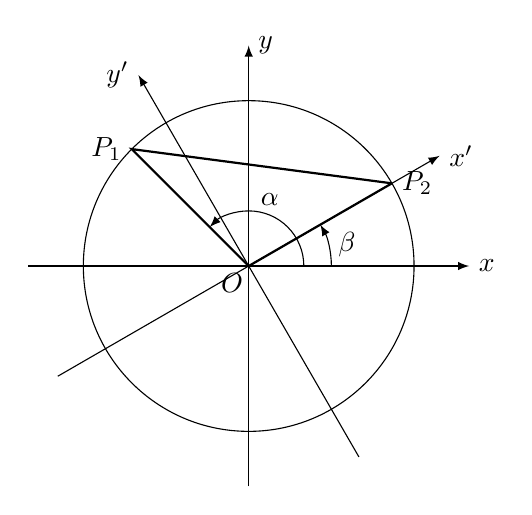
\begin{tikzpicture}[>=latex, scale=.7]
\draw[->] (-4,0)--(4,0)node[right]{$x$};
\draw[->] (0,-4)--(0,4)node[right]{$y$};
\draw (0,0) circle (3);
\draw [->] (210:4)--(30:4)node[right]{$x'$};
\draw [<-] (120:4)node[left]{$y'$}--(-60:4); 
\draw[thick](30:3)node[right]{$P_2$}--(135:3)node[left]{$P_1$}--(0,0)--(30:3);
\draw[->] (1.5,0) arc (0:30:1.5);
\draw [->] (1,0) arc (0:135:1);
\node at (67.5:1)[above]{$\alpha$};
\node at (15:1.5)[right]{$\beta$};
\node at (-.3,-.3){$O$};


    \end{tikzpicture}
    \caption{}
\end{figure}

把$Ox$轴旋转到$\beta$的终边位置而成$Ox'$轴,$Oy$轴旋转同样的角而成$Oy'$轴,
我们用两种方法计算弦长$P_1$, $P_2$。

在$x'Oy'$坐标系中,$P_1$, $P_2$的坐标是
\[P_1\; \left(\cos(\alpha-\beta),\, \sin(\alpha-\beta)\right),\qquad P_2\; (1,0) \]
利用两点间距离公式,得:
\begin{equation}
\begin{split}
|P_1P_2|^2 &=\left[\cos(\alpha-\beta)-1\right]^2+\left[\sin(\alpha-\beta)-0\right]^2\\
&=\cos^2(\alpha-\beta)-2\cos(\alpha-\beta)+1+\sin^2(\alpha-\beta)\\
&=2-2\cos (\alpha-\beta)
\end{split}
\end{equation}

在$xOy$坐标系中,$P_1$, $P_2$的坐标是
\[P_1\;(\cos\alpha,\, \sin\alpha),\qquad  P_2\; (\cos\beta,\, \sin\beta)\]
利用两点间距离公式,得:
\begin{equation}
    \begin{split}
    |P_1P_2|^2 &=(\cos\alpha-\cos\beta)^2+(\sin\alpha-\sin\beta)^2\\
    &=\cos^2\alpha-2\cos\alpha\cos\beta+\cos^2\beta +\sin^2\alpha-2\sin\alpha\sin\beta+\sin^2\beta\\
    &=2-2(\cos\alpha\cos\beta+\sin\alpha\sin\beta)
    \end{split}
    \end{equation}

    在两个坐标系下,弦长是不变的,比较(1.3)式和(1.4)式,即得
   \[ \cos (\alpha-\beta) =\cos\alpha\cos\beta+\sin\alpha\sin\beta\]
    这就是我们所要证明的。
\end{proof}

既然公式(1.2)对任意$\alpha$, $\beta$都成立,则以$-\beta$代替$\beta$, 也必成立
    \[ \cos [\alpha-(-\beta)] =\cos\alpha\cos(-\beta)+\sin\alpha\sin(-\beta)\]

再注意三角函数的奇偶性,就得到
\[ \cos(\alpha+\beta) =\cos\alpha\cos\beta-\sin\alpha\sin\beta\]
这就是我们所要证明的公式(1.1)。

\begin{example}
不查表,求$\cos15^{\circ}$, $\cos75^{\circ}$的值。
\end{example}

\begin{solution}
由于:$15^{\circ}=45^{\circ}-30^{\circ},\qquad 75^{\circ}=45^{\circ}+30^{\circ}$
\[\cos 45^{\circ}=\sin 45^{\circ}=\frac{\sqrt{2}}{2},\quad \cos 30^{\circ}=\frac{\sqrt{3}}{2},\quad \sin 30^{\circ}=\frac{1}{2} \]
所以:
\[\begin{split}
\cos15^{\circ}&=\cos(45^{\circ}-30^{\circ})=\cos 45^{\circ}\cos30^{\circ}+\sin 45^{\circ}\sin30^{\circ}\\
&=\frac{\sqrt{2}}{2}\cdot \frac{\sqrt{3}}{2}+\frac{\sqrt{2}}{2}\cdot \frac{1}{2}\\
&=\frac{\sqrt{6}+\sqrt{2}}{4}\approx 0.9659 
\end{split}\]
\[\begin{split}
\cos75^{\circ}&=\cos(45^{\circ}+30^{\circ})=\cos 45^{\circ}\cos30^{\circ}-\sin 45^{\circ}\sin30^{\circ}\\
&=\frac{\sqrt{2}}{2}\cdot \frac{\sqrt{3}}{2}-\frac{\sqrt{2}}{2}\cdot \frac{1}{2}\\
&=\frac{\sqrt{6}-\sqrt{2}}{4}\approx \frac{2.4495-1.4142}{4}\\
&\approx 0.2588 
\end{split}\]
\end{solution}

\begin{example}
    已知$\sin\alpha=\frac{2}{3}$, $\cos\beta=-\frac{3}{4}$, 并且$\alpha$是第二象限的角,$\beta$是第三象限的角,求$\cos(\alpha-\beta)$的值(准确到0.01)。
\end{example}

\begin{solution}
因为$\alpha$是第二象限的角,所以
\[\cos\alpha=-\sqrt{1-\sin^2\alpha}=-\sqrt{1-\left(\frac{2}{3}\right)^2}=-\frac{\sqrt{5}}{3}\]
因为$\beta$是第三象限的角,所以
\[\sin\beta=-\sqrt{1-\cos^2\beta}=-\sqrt{1-\left(\frac{3}{4}\right)^2}=-\frac{\sqrt{7}}{4}\]
因此:
\[\begin{split}
    \cos (\alpha-\beta) &=\cos\alpha\cos\beta+\sin\alpha\sin\beta\\
    &=\left(-\frac{\sqrt{5}}{3}\right)\left(-\frac{3}{4}\right)+\frac{2}{3}\left(-\frac{\sqrt{7}}{4}\right)\\
    &=\frac{3\sqrt{5}-2\sqrt{7}}{12}\\
    &\approx \frac{3\times2.236-2\times 2.646}{12}\approx 0.12
\end{split}\]
\end{solution}


\begin{example}
证明对于任何角$\alpha$,以下公式成立
\[\cos\left(\frac{\pi}{2}-\alpha\right)=\sin \alpha,\qquad \sin\left(\frac{\pi}{2}-\alpha\right)=\cos \alpha\]
\end{example}

\begin{proof}
利用公式(1.2),可得:
\[\cos\left(\frac{\pi}{2}-\alpha\right)=\cos\frac{\pi}{2}\cdot \cos\alpha+\sin\frac{\pi}{2}\cdot \sin \alpha\]
但是
\[\cos\frac{\pi}{2}=0,\qquad \sin\frac{\pi}{2}=1\]
所以$\cos\left(\frac{\pi}{2}-\alpha\right)=\sin\alpha$

又因为上式中的$\alpha$为任意角,所以,若把公式中的$\left(\frac{\pi}{2}\right)$换成$\alpha$,就可得
\[\cos\alpha=\sin\left(\frac{\pi}{2}-\alpha\right)\]
即:$\sin\left(\frac{\pi}{2}-\alpha\right)=\cos\alpha$
\end{proof}

\begin{ex}
\begin{enumerate}
    \item 等式$\cos(\alpha+\beta)=\cos\alpha+\cos\beta$成立吗?
    为什么?试举例说明
    
    \item 不查表,求下列各式的值:
    \begin{tasks}(2)
        \task $\cos135^{\circ}$
        \task $\cos\left(\frac{-61\pi}{12}\right)$
        \task $\cos1950^{\circ}$
        \task $\cos\frac{4\pi}{9} \cos\frac{\pi}{9}\sin\frac{4\pi}{9}\sin \frac{\pi}{9}$
        \task $\cos^2 15^{\circ}-\sin^2 15^{\circ}$
    \end{tasks}        

\item 已知$\cos\theta=-\frac{5}{13}$, $\theta$为II象限角,试求$\cos\left(\frac{\pi}{3}-\theta\right)$,
    $\cos\left(\theta+\frac{\pi}{6}\right)$的值。
    \item 证明:$\alpha$为任意角时,下式成立。
\[\cos\left(\frac{3\pi}{2}-\alpha\right)=-\sin\alpha,\qquad \cos(\pi+\alpha)=-\cos\alpha  \]
\end{enumerate}
\end{ex}


\subsection{两角和与差的正弦}
\begin{blk}{定理2}
两个任意角$\alpha$和$\beta$的和(差)的正弦等于第一
个角的正弦乘以第二个角的余弦的积加上(减去)第一角的余弦乘以第二个角的正弦的乘积。即
\begin{align}
    \sin (\alpha+\beta) &=\sin\alpha\cos\beta+\cos\alpha\sin\beta \\
    \sin (\alpha-\beta) &=\sin\alpha\cos\beta-\cos\alpha\sin\beta
\end{align}
\end{blk}

\begin{proof}
因为已经知道
\[\cos\left(\frac{\pi}{2}+\alpha\right)=-\sin\alpha,\qquad \sin\left(\frac{\pi}{2}+\alpha\right)=\cos\alpha\]
所以
\[\begin{split}
 \sin(\alpha+\beta) &=-\cos\left[\frac{\pi}{2}+(\alpha+\beta)\right]\\
 &=-\cos\left[\left(\frac{\pi}{2}+\alpha\right)+\beta\right]\\
&=-\left[\cos\left(\frac{\pi}{2}+\alpha\right)\cos\beta-\sin\left(\frac{\pi}{2}+\alpha\right)\sin\beta\right]\\    
&=-\left(-\sin\alpha\cos\beta-\cos\alpha\sin\beta\right)\\
&=\sin\alpha\cos\beta+\cos\alpha\sin\beta
\end{split}\]
以$(-\beta)$替换公式(1.5)中的$\beta$,得到
\[\begin{split}
  \sin(\alpha-\beta)&=\sin\alpha\cos(-\beta)+\cos\alpha\sin(-\beta)\\
  &=\sin\alpha\cos\beta-\cos\alpha\sin\beta  
\end{split}\]
\end{proof}

\begin{example}
    求$\sin15^{\circ}$和$\sin75^{\circ}$。(不查表)
\end{example}

\begin{solution}
    \[\begin{split}
        \sin 15^{\circ}&=\sin (45^{\circ}-30^{\circ})\\
        &=\sin45^{\circ}\cos30^{\circ}-\cos45^{\circ}\sin30^{\circ}\\
        &=\frac{\sqrt{2}}{2}\cdot\frac{\sqrt{3}}{2}-\frac{\sqrt{2}}{2}\cdot\frac{1}{2}\\
        &=\frac{\sqrt{6}-\sqrt{2}}{4}
    \end{split}\]
    (这就是$\cos75^{\circ}$的值)。
    \[\begin{split}
        \sin 75^{\circ}&=\sin (45^{\circ}+30^{\circ})\\
        &=\sin45^{\circ}\cos30^{\circ}+\cos45^{\circ}\sin30^{\circ}\\
        &=\frac{\sqrt{2}}{2}\cdot\frac{\sqrt{3}}{2}+\frac{\sqrt{2}}{2}\cdot\frac{1}{2}\\
        &=\frac{\sqrt{6}+\sqrt{2}}{4}  
    \end{split}\]
    (这就是$\cos15^{\circ}$的值)。
\end{solution}

\begin{example}
已知$\cos\phi=\frac{3}{5}$,且$\phi$是第四象限角,试求$\sin\left(\phi-\frac{\pi}{6}\right)$的值。
\end{example}

\begin{solution}
因为$\phi$为第四象限角,所以
\[\sin\phi=-\sqrt{1-\left(\frac{3}{5}\right)^2}=-\frac{4}{5}\]
于是
\[\begin{split}
    \sin\left(\phi-\frac{\pi}{6}\right)&=\sin\phi\cos\frac{\pi}{6}-\cos\phi\sin\frac{\pi}{6}\\
    &=-\frac{4}{5}\cdot \frac{\sqrt{3}}{2}-\frac{3}{5}\cdot\frac{1}{2}\\
    &=-\frac{4\sqrt{3}+3}{10}
\end{split}\]
\end{solution}

\begin{example}
    求证:$\frac{\sin(\alpha+\beta)\cdot \sin(\alpha-\beta)}{\sin^2\alpha\cdot \sin^2\beta}=\cot^2\beta-\cot^2\alpha$
\end{example}

\begin{proof}
\[\begin{split}
\text{等式左边}&=\frac{(\sin\alpha\cos\beta+\cos\alpha\sin\beta)(\sin\alpha\cos\beta-\cos\alpha\sin\beta)}{\sin^2\alpha\cdot \sin^2\beta}\\
&=\frac{\sin^2\alpha\cdot \cos^2\beta-\cos^2\alpha\cdot \sin^2\beta}{\sin^2\alpha\cdot \sin^2\beta}\\
&=\cot^2\beta-\cot^2\alpha=\text{等式右边}
\end{split}\]
\end{proof}

\begin{example}
求证$\sin\theta+\cos\theta=\sqrt{2}\sin\left(\theta+\frac{\pi}{4}\right)$
\end{example}

\begin{proof}
可用不同方法证之。

\textbf{证法1:}
\[\begin{split}
\text{左边}&=\sqrt{2}\left(\frac{\sqrt{2}}{2}\sin\theta+\frac{\sqrt{2}}{2}\cos\theta\right)\\
&=\sqrt{2}\left(\sin\theta\cdot \cos\frac{\pi}{4}+\cos\theta\cdot\sin\frac{\pi}{4}\right)\\
&=\sqrt{2}\sin\left(\theta+\frac{\pi}{4}\right)=\text{右边}    
\end{split}\]

\textbf{证法2:}
\[\begin{split}
\text{右边}&=\sqrt{2}\left(\sin\theta\cdot \cos\frac{\pi}{4}+\cos\theta\cdot\sin\frac{\pi}{4}\right)\\
&=\sqrt{2}\left(\frac{\sqrt{2}}{2}\sin\theta+\frac{\sqrt{2}}{2}\cos\theta\right)\\
&=\sin\theta+\cos\theta=\text{左边}
\end{split}\]
\end{proof}


\begin{ex}
\begin{enumerate}
    \item 你能知道当$\alpha,\beta$取何值时,等式
    $\sin(\alpha+\beta)=\sin\alpha+\sin\beta$能够成立呢?
\item 不查表,求下式的值
\begin{enumerate}
    \item $\sin 105^{\circ}$
    \item $\sin\left(-\frac{5\pi}{12}\right)$
    \item $\tan 15^{\circ}$
    \item $\sin 14^{\circ}\cdot \cos 16^{\circ}+\cos 14^{\circ}\cdot \sin 16^{\circ}$
    \item $\sin 79^{\circ}\cdot \cos 25^{\circ}-\sin 20^{\circ}\cdot \sin 25^{\circ}$
\end{enumerate}
\item 已知$\sin\alpha=\frac{2}{3}$, $\cos\beta=-\frac{3}{4}$,且$\alpha,\beta$都是第二象限角

试求
$\sin(\alpha+\beta)$与$\cos(\alpha-\beta)$的值。
\item 求证:
\begin{enumerate}
    \item $\sin\left(\frac{5\pi}{6}-\phi\right)+\sin\left(\frac{5\pi}{6}+\phi\right)=\cos\phi$
    \item $2\cos(60^{\circ}-\alpha)-\sqrt{3}\sin\alpha=\cos\alpha$
\end{enumerate}
\end{enumerate}
\end{ex}

\subsection{两角和与差的正切}
\begin{blk}{定理3}
    两个角$\alpha$与$\beta$的和(或差)的正切,等于一个
分式,其分子为这两角正切的和(或整),其分母为1与这两个角的正切乘积的差(或和)。即
\begin{align}
    \tan(\alpha+\beta)&=\frac{\tan\alpha+\tan\beta}{1-\tan\alpha\tan\beta}\\
    \tan(\alpha-\beta)&=\frac{\tan\alpha-\tan\beta}{1+\tan\alpha\tan\beta}
\end{align}
\end{blk}

\begin{rmk}
    在这两个公式中,必须保证$\tan\alpha$, $\tan\beta$及$\tan(\alpha\pm\beta)$都有意义,因而,当且仅当$\alpha,\beta,\alpha\pm\beta$, 都不等于$\frac{\pi}{2}+k\pi\; (k\in\mathbb{Z})$时,公式才能成立。
\end{rmk}

\begin{proof}
    对于公式(1.7)利用公式$\tan(\alpha+\beta)=
\frac{\sin (\alpha+\beta)}{\cos (\alpha+\beta)}$,和关于正弦函数与余弦函数的加法定理,得:
\[\tan(\alpha+\beta)=\frac{\sin\alpha\cos\beta+\cos\alpha\sin\beta}{\cos\alpha\cos\beta-\sin\alpha\sin\beta} \]

用$\cos\alpha\cos\beta$除右端的分子和分母,得:
\[\begin{split}
    \tan(\alpha+\beta)&=\frac{\frac{\sin\alpha\cos\beta}{\cos\alpha\cos\beta}+\frac{\cos\alpha\sin\beta}{\cos\alpha\cos\beta}}{\frac{\cos\alpha\cos\beta}{\cos\alpha\cos\beta}-\frac{\sin\alpha\sin\beta}{\cos\alpha\cos\beta}}\\
&=\frac{\frac{\sin\alpha}{\cos\alpha}+\frac{\sin\beta}{\cos\beta}}{1-\frac{\sin\alpha\sin\beta}{\cos\alpha\cos\beta}}\\
&=\frac{\tan\alpha+\tan\beta}{1-\tan\alpha\tan\beta}
\end{split}\]
对于公式(1.8),
\[\begin{split}
    \tan(\alpha-\beta)&=\tan[\alpha+(-\beta)]\\
    &=\frac{\tan\alpha+\tan(-\beta)}{1-\tan\alpha\tan(-\beta)}\\
    &=\frac{\tan\alpha-\tan\beta}{1+\tan\alpha\tan\beta}
\end{split} \]
\end{proof}

\begin{example}
    求$\tan15^{\circ}$和$\tan75^{\circ}$的值。
\end{example}

\begin{solution}
\[\begin{split}
    \tan15^{\circ}&=\tan (60^{\circ}-45^{\circ})\\
&=\frac{\tan 60^{\circ}-\tan 45^{\circ}}{1+\tan 60^{\circ}\tan45^{\circ}}\\
&=\frac{\sqrt{3}-1}{1+\sqrt{3}}=\frac{(\sqrt{3}-1)^2}{2}\\
&=\frac{4-2\sqrt{3}}{2}=2-\sqrt{3}
\end{split}\]
\[\begin{split}
    \tan 75^{\circ}&=\tan (45^{\circ}+30^{\circ})\\
&=\frac{1+\frac{1}{\sqrt{3}}}{1-\frac{1}{\sqrt{3}}}=\frac{\sqrt{3}+1}{\sqrt{3}-1}\\
&=\frac{4+2\sqrt{3}}{2}=2+\sqrt{3}
\end{split}\]
\end{solution}


\begin{example}
求两角和及差的余切公式。
\end{example}

\begin{solution}
 因为余切是正切的倒数,则用$\tan\alpha$和$\tan\beta$表示
    $\cot (\alpha+\beta)$和$\cot(\alpha-\beta)$的公式,可以从(1.7)和(1.8)中交换第一个分子和分母的位置而得,我们得出公式:
\[    \cot (\alpha+\beta)=\frac{1-\tan\alpha\cdot\tan \beta}{\tan\alpha+\tan \beta}\]
   
等式右边的分子、分母同除以$\tan\alpha\cdot\tan\beta\ne 0$得到 
\begin{equation}
    \cot(\alpha+\beta)=\frac{\cot\alpha\cot\beta-1}{\cot\alpha+\cot\beta}
\end{equation}
以$(-\beta)$替换上面等式中的$\beta$,得到
\[
    \cot(\alpha-\beta)=\frac{\cot\alpha\cot(-\beta)-1}{\cot\alpha+\cot(-\beta)}=\frac{\cot\alpha\cot\beta+1}{\cot\beta-\cot\alpha}
\]
所以
\begin{equation}
    \cot(\alpha-\beta)=\frac{\cot\alpha\cot\beta+1}{\cot\beta-\cot\alpha}  
\end{equation}
式中$\alpha,\beta,\alpha\pm\beta$都不等于$k\pi$。($k$为任何整数)
\end{solution}

\begin{example}
已知$\tan\alpha=\frac{1}{3}$, $\cot\beta=-\frac{1}{2}$,试求:
\begin{enumerate}
    \item $\cot(\alpha-\beta)$的值。
    \item $\alpha+\beta$的值,其中$0<\alpha<\frac{\pi}{3},\quad \frac{\pi}{2}<\beta<\pi$
\end{enumerate}
\end{example}

\begin{solution}
\begin{enumerate}
    \item 因为$\tan\alpha=\frac{1}{3}$, $\tan\beta=\frac{1}{\cot\beta}=-2$,以及
\[\cot(\alpha-\beta)=\frac{1}{\tan(\alpha-\beta)}=\frac{1+\tan\alpha\cdot \tan\beta}{\tan\alpha-\tan\beta}\]
所以
\[\cot(\alpha-\beta)=\frac{1-\frac{2}{3}}{\frac{1}{3}+2}=\frac{1}{7} \]

\item 由于$\tan(\alpha+\beta)=\frac{\tan \alpha+\tan\beta}{1-\tan\alpha\cdot \tan\beta}=-1$,而且$0<\alpha<\frac{\pi}{3}$, $\frac{\pi}{2}<\beta<\pi$,因而可得$\frac{\pi}{2}<\alpha+\beta<\frac{3\pi}{2}$

在$\frac{\pi}{2}$与$\frac{3\pi}{2}$之间,只有$\tan\frac{3\pi}{4}=-1$,所以
\[\alpha+\beta =\frac{3\pi}{4}\]
\end{enumerate}    
\end{solution}

\begin{example}
求证$\frac{1+\tan 75^{\circ}}{1-\tan 75^{\circ}}=-\sqrt{3}$
\end{example}

\begin{analyze}
如果利用$\tan45^{\circ}=1$这个等式,再考虑等式左边可变形为
\[\frac{\tan 45^{\circ}+\tan 75^{\circ}}{1-\tan 45^{\circ}\cdot \tan 75^{\circ}}\]
这样,利用两角和的正切公式经过化简,正好是一个特殊角$120^{\circ}$的正切,它的值可求得。
\end{analyze}

\begin{proof}
注意$1=\tan 45^{\circ}$,所以
\[\text{左边}=\frac{\tan 45^{\circ}+\tan 75^{\circ}}{1-\tan 45^{\circ}\cdot \tan 75^{\circ}}=\tan 120^{\circ}=-\sqrt{3}=\text{右边}\]
\end{proof}


\begin{example}
    已知:$\tan\left(\frac{\pi}{4}+\alpha\right)=m$,求$\tan\alpha$的值。
\end{example}

\begin{solution}
\textbf{解法1:} 由已知,$\alpha\ne \frac{\pi}{4}+k\pi\; (k\in\mathbb{Z})$。不然的话,$\alpha+\frac{\pi}{4}=\frac{pi}{2}+k\pi$, $\tan\left(\frac{\pi}{4}+\alpha\right)$就没有意义了。

所以$\tan\left(\frac{\pi}{4}+\alpha\right)=\frac{1+\tan\alpha}{1-\tan\alpha}=m$

由于$1-\tan\alpha\ne 0$,所以由上式可得
\[1+\tan\alpha=m-m\tan\alpha\]
即:$(m+1)\tan\alpha=m-1$
所以:$\tan\alpha=\frac{m-1}{m+1},\quad (m\ne -1)$

\textbf{解法2:} 因为$\alpha=\left(\frac{\pi}{4}+\alpha\right)-\frac{\pi}{4}$,所以
\[\begin{split}
   \tan \alpha&=\tan\left[\left(\frac{\pi}{4}+\alpha\right)-\frac{\pi}{4}\right] \\
   &=\frac{\tan\left(\frac{\pi}{4}+\alpha\right)-\tan\frac{\pi}{4}}{1+\tan\left(\frac{\pi}{4}+\alpha\right)\cdot \tan\frac{\pi}{4}}\\
   &=\frac{m-1}{m+1}\quad (m\ne -1)
\end{split}\]
\end{solution}



\begin{example}
设$\cot\alpha, \cot\beta$是一元二次方程$ax^2+bx+c=0\quad (a\ne c\ne 0)$的两个根,试求$\tan (\alpha+\beta)$的值。
\end{example}

\begin{solution}
由韦达定理知
\[\cot\alpha+\cot\beta=-\frac{b}{a},\qquad \cot\alpha\cdot \cot\beta=\frac{c}{a}\]    
即:
\[\frac{\tan\alpha+\tan\beta}{\tan\alpha\cdot \tan\beta}=-\frac{b}{a},\qquad \frac{1}{\tan\alpha\cdot \tan\beta}=\frac{c}{a}\]  
由此两式可以求得 
\[\tan\alpha+\tan\beta=-\frac{b}{c},\qquad \tan\alpha\cdot \tan\beta=\frac{a}{c}\]
所以:
\[\tan(\alpha+\beta)=\frac{\tan\alpha+\tan\beta}{1-\tan\alpha\cdot \tan\beta}=\frac{-\frac{b}{c}}{1-\frac{a}{c}}=\frac{b}{a-c}\]
\end{solution}

\begin{ex}
\begin{enumerate}
    \item 不查表,求值:
\begin{tasks}(2)
    \task $\tan 435^{\circ}$
    \task $\cot 105^{\circ}$
    \task $\frac{\tan 17^{\circ}+\tan 28^{\circ}}{1+\tan 17^{\circ}\cdot \tan 152^{\circ}}$
    \task $\frac{1+\tan 15^{\circ}}{\tan 15^{\circ}-1}$
\end{tasks}

\item 已知$\tan\alpha=2$,且$\alpha\in\left(\pi,\frac{3\pi}{2}\right)$,试求$\tan\left(\alpha-\frac{\pi}{4}\right)$的值。
\item 若$\alpha,\beta$都是锐角,且$\tan\alpha=2$, $\cot\beta=\frac{1}{3}$。求证:$\alpha+\beta =135^{\circ}$。
\end{enumerate} 
\end{ex}

\section*{习题1.1}
\addcontentsline{toc}{subsection}{习题1.1}
\begin{enumerate}
\item 已知$\sin\alpha=\frac{15}{17}$, $\cos\beta=-\frac{5}{13}$, 且$\alpha$, $\beta$都是第二象限角,试求$\cos(\alpha+\beta)$, $\cos(\alpha-\beta)$的值。
\item 在$\triangle ABC$中,$\cos A=\frac{4}{5}$, $\cos B=\frac{12}{13}$, 试求 $\cos C$的值。
\item 求证:
\begin{enumerate}
    \item $\cos (\alpha+60^{\circ}) +\cos (\alpha-60^{\circ}) =\cos\alpha$
    \item $\cos (\alpha+\beta)\cdot \cos\beta+\sin\beta\cdot \sin(\alpha+\beta) =\cos\alpha$
    \item $\cos (\alpha+\beta)\cdot \cos (\alpha-\beta) =\cos^2\alpha+\cos^2\beta-1$
\end{enumerate}
\item 化简下列各式:
\begin{enumerate}
    \item $\cos\left(\frac{\pi}{6}+\alpha\right)-\cos\left(\frac{\pi}{6}-\alpha\right)$
    \item $\frac{\cos\alpha\cdot \cos\beta-\cos (\alpha+\beta)}{\cos (\alpha-\beta)-\sin\alpha\cdot \sin\beta}$
    \item $\frac{\cos (\alpha+\beta)+\cos(\alpha-\beta)}{\cos (\alpha+\beta)-\cos (\alpha-\beta)}$
    \item $\cos25^{\circ}\cdot \cos29^{\circ}-\sin24^{\circ}\cdot \sin29^{\circ}$
    \item $\cos (36^{\circ}+x)\cdot \cos (54^{\circ}-x)\sin (36^{\circ}+x)\cdot \sin (54^{\circ}-x)$
\end{enumerate} 

\item 已知$\cos\alpha=\cos\beta=m$, $\sin\alpha=\sin\beta=n$, 试求$\cos(\alpha+\beta)$及$\cos(\alpha-\beta)$的值,并求出$m$与$n$的关系式。
\item 求下列各函数的值(不查表):
\[\sin150^{\circ},\qquad \sin195^{\circ},\qquad -\tan 195^{\circ}\]
\item 已知$\cos\alpha=-\frac{8}{17}$, $\cos\beta=\frac{4}{5}$,
且$\alpha$是第二象限角,$\beta$
是第四象限角,试求$\sin(\alpha+\beta)$

\item 若$\cos\alpha=-\frac{3}{15}$, $\sin\beta=\frac{8}{17}$, 且$a\in\left(\pi,\frac{3\pi}{2}\right)$,
$\beta\in \left(0,\frac{\pi}{2}\right)$, 试求$\sin(\alpha-\beta)$.


\item 若$\cos\alpha=\frac{1}{7}$, $\cos(\alpha+\beta)=-\frac{11}{14}$, 且$0<\alpha<\frac{\pi}{2}$。试求角$\beta$的值。

\item 化简下列各式:
\begin{enumerate}
    \item $\sin13^{\circ}\cdot\cos17^{\circ}+\cos13^{\circ}\cdot \sin163^{\circ}$
    \item $\sin70^{\circ}\cdot\sin65^{\circ}-cos70^{\circ}\cdot\sin25^{\circ}$
    \item $\sin\left(\alpha+\frac{\pi}{3}\right)+\sin\left(\alpha-\frac{\pi}{3}\right)$
    \item $\frac{\sin(\beta-\gamma)+\sin(\beta+\gamma)}{\sin(\beta+\gamma)-\sin(\beta-\gamma)}$
    \item $\frac{\sin(\beta-\gamma)}{\cos\beta\cdot \cos\gamma}+\frac{\sin(\gamma-\alpha)}{\cos\gamma\cdot \cos\alpha}+\frac{\sin(\alpha-\beta)}{\cos\alpha\cdot \cos\beta}$
\end{enumerate}

\item 已知$\sin\alpha=\frac{3}{4}$, 且$\frac{\pi}{2}<\alpha<\pi$,求$\tan\left(\frac{\pi}{3}+\alpha\right)$
\item \begin{enumerate}
    \item 已知$\tan x=\frac{1}{4}$, $\tan y=-3$, 求$\tan(x+y)$的值;
    \item 已知$\tan \alpha=2k+1$, $\tan\beta=2k-1$, 求$\cot(\alpha-\beta)$的值.
\end{enumerate}

\item 求证:
\begin{enumerate}
    \item $\tan(x+y)\cdot \tan(x-y)=\frac{\tan^2 x-\tan^2 y}{1-\tan^2 x\cdot \tan^2 y}$
    \item $\frac{1-\tan\theta}{1+\tan\theta}=\cot\left(\theta+\frac{\pi}{4}\right)$
\item $\frac{\tan x+\tan y}{\tan x-\tan y}=\frac{\sin(x+y)}{\sin(x-y)}$
\end{enumerate}

\item 已知$\theta, \phi$都是锐角,且$\tan \theta=\frac{1}{2}$, $\tan\phi=\frac{1}{3}$, 求证:
$\theta+\phi=45^{\circ}$。

\item 如图1.2,矩形$ABCD$被划分成三个全等的正方形。求证:
\begin{enumerate}
    \item $\angle \theta=\angle \gamma$
    \item $\alpha+\beta+\gamma=90^{\circ}$
\end{enumerate}

\begin{figure}[htp]
    \centering
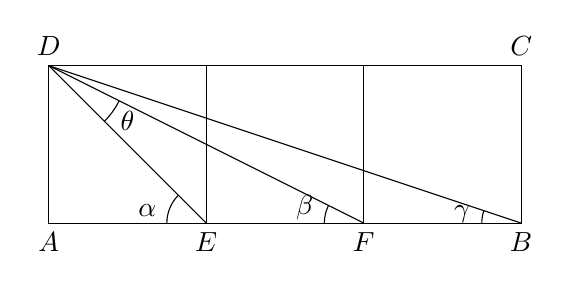
\begin{tikzpicture}
\draw (0,0)node[above]{$D$} rectangle (6,-2);
\draw (0,0) rectangle (4,-2);
\draw (0,0) rectangle (2,-2);
\foreach \x/\xtext in {0/A,2/E,4/F,6/B}
{
    \node at (\x,-2)[below]{$\xtext$};
}
\node at (6,0)[above]{$C$};

\foreach \x/\xtext in {2/45,4/26.56,6/18.43}
{
    \draw (\x-.5,-2) arc (180:180-\xtext:.5);
}

\foreach \x/\xtext in {2/\alpha,4/\beta,6/\gamma}
{
    \draw (0,0) --(\x,-2);
\node at (\x-.75,-2-.02*\x)[above]{$\xtext$};
}
\draw (360-45:1) arc (360-45:360-45+18.43:1);
\node at (1,-.7){$\theta$};
\end{tikzpicture}
    \caption{}
\end{figure}

\item 若$\sin\alpha=\frac{\sqrt{10}}{10}$, $\tan\beta=-\frac{1}{2}$. $90^{\circ}<\alpha<180^{\circ}$, $90^{\circ}<\beta<180^{\circ}$,求证:
\begin{enumerate}
    \item $\tan(\alpha+\beta)=-1$
    \item $\alpha+\beta=315^{\circ}$
\end{enumerate}

\item 已知$\cot\alpha=\frac{3}{4}$, $\cot\beta=\frac{1}{7}$,
且$\alpha,\beta$都是锐角,

求证:$1+\beta=135^{\circ}$。

\item 已知$\tan\alpha$与$\tan\beta$是方程$x^2+6x+7=0$的两个根。

求证:$\sin(\alpha+\beta) =\cos(\alpha+\beta)$

\item 已知 $a\cdot\sin(\theta+x)=b\sin(\theta+y)$, 求证:
\[\tan\theta=\frac{b\sin y-a\sin x}{a\cos x-b\cos y}\]

\end{enumerate}

\section{二倍角的正弦、余弦和正切}
\subsection{二倍角的正弦、余弦和正切}

在两角和的正弦、余
弦和正切的公式中,
令$\beta=\alpha$,则得到
\[\sin(\alpha+\alpha)=\sin\alpha\cos\alpha+\cos\alpha\sin\alpha\]
即
\begin{equation}
    \sin2\alpha=2\sin\alpha\cos\alpha
\end{equation}
\[\cos(\alpha+\alpha)=\cos\alpha\cos\alpha-\sin\alpha\sin\alpha\]
即
\begin{equation}
    \cos2\alpha=\cos^2\alpha-\sin^2\alpha
\end{equation}
若在公式(1.12)中,用$1-sin^2\alpha$代换 $\cos^2\alpha$, 或用$1-\cos^2\alpha$代换$\sin^2\alpha$, 则对于$\cos2\alpha$又得到两个公式
\begin{align}
    \cos2\alpha&=1-2\sin^2\alpha\\
    \cos2\alpha&=2\cos^2\alpha-1 
\end{align}
\[\tan (\alpha+\alpha)=\frac{\tan\alpha+\tan\alpha}{1-\tan\alpha\tan\alpha}\]
即:
\begin{equation}
    \tan2\alpha=\frac{2\tan\alpha}{1-\tan^2\alpha}
\end{equation}

\begin{rmk}
\begin{enumerate}
    \item 二倍角的三角函数的公式是把任意角的三角函数与小一半的角的三角函数联系起来,它们可以写成下面的各种形式的等式。例如
\[\begin{split}
    \sin4\alpha&=\sin2\cdot (2\alpha) =2\sin2\alpha\cos2\alpha\\
    \sin\alpha&=\sin2\left(\frac{\alpha}{2}\right)=2\sin\frac{\alpha}{2}\cos \frac{\alpha}{2}\\
    \cos\frac{\alpha}{2}&=\cos^2\frac{\alpha}{4}-\sin^2\frac{\alpha}{4}\\
    \tan3\alpha&=\frac{2\tan\frac{3\alpha}{2}}{1-\tan^2\frac{3\alpha}{2}}
\end{split}\]

\item 在二倍的正切公式(1.15)中,除了$\alpha=\frac{\pi}{2}+k\pi$和$\alpha=\frac{\pi}{4}+\frac{k\pi}{2},\; (k\in\mathbb{Z})$
诸值之外,对$\alpha$的其余一切值都成立,因为当所指定的那些$\alpha$值,$\tan\alpha$和$\tan2\alpha$都不存在。
\item 在使用二倍角三角函数的公式作恒等变形时,不仅要掌握从等式的左端的式子变换到右端的式子,而且也要熟练地掌握从等式的右端的式子变换到左端的式子。
\end{enumerate}
\end{rmk}

\begin{example}
    化简下面的式子
\begin{tasks}(2)
    \task $4\sin 15^{\circ}\cos 15^{\circ}$
    \task $\frac{1}{2}\sin 15^{\circ}\sin 255^{\circ}$
    \task $\cos^2\frac{\pi}{8}-\sin^2\frac{\pi}{8}$
    \task $\cos^2 15^{\circ}-\frac{1}{2}$
    \task $\frac{\tan 75^{\circ}}{1-\tan^2 75^{\circ}}$
\end{tasks}
\end{example}

\begin{solution}
\begin{enumerate}
    \item $4\sin 15^{\circ}\cos 15^{\circ}=2\sin 30^{\circ}=1$
    \item $\frac{1}{2}\sin 15^{\circ}\sin 255^{\circ}=-\frac{1}{2}\sin 15^{\circ}\cos 15^{\circ}=-\frac{1}{4}\sin 30^{\circ}=-\frac{1}{8}$
    \item $\cos^2\frac{\pi}{8}-\sin^2\frac{\pi}{8}=\cos\frac{\pi}{4}=\frac{\sqrt{2}}{2}$
    \item $\cos^2 15^{\circ}-\frac{1}{2}=\frac{2\cos^2 15^{\circ}-1}{2}=\frac{\cos 30^{\circ}}{2}=\frac{\sqrt{3}}{4}$
    \item $\frac{\tan 75^{\circ}}{1-\tan^2 75^{\circ}}=\frac{1}{2}\frac{2\tan 75^{\circ}}{1-\tan^2 75^{\circ}}=\frac{1}{2}\tan 150^{\circ}=-\frac{1}{2}\tan 30^{\circ}=-\frac{\sqrt{3}}{6}$
\end{enumerate}    
\end{solution}

\begin{example}
    已知$0^{\circ}<\alpha<90^{\circ}$, $0^{\circ}<\beta<90^{\circ}$, $\tan\alpha=\frac{1}{7}$,
    $\sin\beta=\frac{1}{\sqrt{10}}$。
    
    求证:$\alpha+2\beta=45^{\circ}$
\end{example}

\begin{figure}[htp]
    \centering
        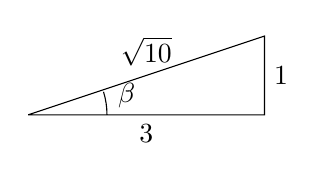
\begin{tikzpicture}
          \draw (0,0)--node[below]{3}(3,0)--node[right]{1}(3,1)--node[above]{$\sqrt{10}$}(0,0);
        \draw (1,0) arc (0:17:1);   
        \node at (1.25,.25){$\beta$};       
        \end{tikzpicture}
    \caption{}
\end{figure}


\begin{solution}
因为$\beta$是锐角,所以$\tan\beta=\frac{1}{3}$,由$\tan\beta<1$知$0^{\circ}<\beta<45^{\circ}$,同理$0^{\circ}<\alpha<45^{\circ}$。

又$\tan2\beta=\frac{\frac{2}{3}}{1-\left(\frac{1}{3}\right)^2}=\frac{3}{4}<1$

所以$0^{\circ}<2\beta <45^{\circ}$,并且
\[\tan(\alpha+2\beta)=\frac{\tan \alpha+\tan2\beta}{1-\tan \alpha\tan2\beta}=\frac{\frac{1}{7}+\frac{3}{4}}{1-\frac{1}{7}\cdot \frac{3}{4}}=1\]
所以$\alpha+2\beta=45^{\circ}+k\cdot 180^{\circ}\; (k\in\mathbb{Z})$,但是因为$0^{\circ}<\alpha<45^{\circ}$,$0^{\circ}<2\beta <45^{\circ}$,所以$0^{\circ}<\alpha+2\beta<90^{\circ}$,因此,$k$只能取0,因而:
\[\alpha+2\beta=45^{\circ}\]
\end{solution}


\begin{example}
用$\alpha$角的三角函数表示$\sin3\alpha$, $\cos3\alpha$和$\tan3\alpha$。
\end{example}



\begin{solution}
\begin{enumerate}
    \item \[\begin{split}
        \sin3\alpha&=\sin(\alpha+2\alpha)=\sin\alpha \cos2\alpha+\cos\alpha\sin2\alpha\\
        &=\sin\alpha(1-2\sin^2\alpha)+2\sin\alpha(1-\sin^2\alpha) \\
        &=\sin\alpha-2\sin^3\alpha+2\sin\alpha-2\sin^3\alpha\\
        &=3\sin\alpha-4\sin^3\alpha     
    \end{split}\]
    \item \[\begin{split}
       \cos3\alpha&=\cos(\alpha+2\alpha)=\cos\alpha\cos2\alpha-\sin\alpha\sin2\alpha\\
       &=\cos\alpha(2\cos^2\alpha-1)-2\cos\alpha(1-\cos^2\alpha)\\
       &=2\cos^3\alpha-\cos\alpha-2\cos\alpha+2\cos^3\alpha\\
       &=4\cos^3\alpha-3\cos\alpha 
    \end{split}\]
    \item \[\begin{split}
\tan3\alpha&=\tan(\alpha+2\alpha)=\frac{\tan\alpha+\tan2\alpha}{1-\tan\alpha\tan2\alpha}\\
&=\frac{\tan\alpha+\frac{2\tan\alpha}{1-\tan^2\alpha}}{1-\tan\alpha\cdot \frac{2\tan\alpha}{1-\tan^2\alpha}}\\
&=\frac{\tan\alpha-\tan^3\alpha+2\tan\alpha}{1-\tan^2\alpha-2\tan^2\alpha}\\
&=\frac{3\tan\alpha-\tan^3\alpha}{1-3\tan^2\alpha}        
    \end{split}\]
\end{enumerate}
\end{solution}

\begin{example}
求证:
\begin{enumerate}
    \item $[\sin\alpha(1-\sin\alpha)+\cos\alpha(1-\cos\alpha)]\times [\sin\alpha(1+\sin\alpha)+\cos\alpha(1+\cos\alpha)]=\sin2\alpha$
    \item $\sin 50^{\circ}\left(1+\sqrt{3}\tan 10^{\circ}\right)=1$
\end{enumerate}
\end{example}

\begin{proof}
\begin{enumerate}
    \item \[\begin{split}
 \text{左边}&=(\sin\alpha-\sin^2\alpha+\cos\alpha-\cos^2\alpha)\times (\sin\alpha+\sin^2\alpha+\cos\alpha+\cos^2\alpha)\\
 &=(\sin\alpha+\cos\alpha-1)(\sin\alpha+\cos\alpha+1)\\
 &=(\sin\alpha+\cos\alpha)^2-1\\
 &=2\sin\alpha\cos\alpha\\
 &=\sin2\alpha=\text{右边}       
    \end{split}\]
    \item \[\begin{split}
\text{左边}&= \sin 50^{\circ} \left(1+\frac{\sqrt{3}\sin 10^{\circ}}{\cos 10^{\circ}}\right)\\       
&= \sin 50^{\circ}\frac{2\left(\frac{1}{2}\cos10^{\circ}+\frac{\sqrt{3}}{2}\sin 10^{\circ}\right)}{\cos 10^{\circ}}\\
&=2\sin 50^{\circ}\cdot \frac{\cos60^{\circ}\cdot \cos10^{\circ}+\sin 60^{\circ}\cdot \sin 10^{\circ}}{\cos10^{\circ}}\\
&=\frac{2\sin50^{\circ}\cdot \cos50^{\circ}}{\cos10^{\circ}}\\
&=\frac{\sin100^{\circ}}{\cos10^{\circ}}\\
&=\frac{\cos10^{\circ}}{\cos10^{\circ}}=1=\text{右边}
    \end{split}\]
\end{enumerate}    
\end{proof}

\begin{ex}
\begin{enumerate}
    \item 不查表,求下列各式的值:
\begin{tasks}(2)
    \task $2\sin12^{\circ}30'\cdot \cos12^{\circ}30'$
    \task $\cos^2\frac{\pi}{12}-\sin^2\frac{\pi}{12}$
    \task $2\cos^2 67^{\circ}30'-1$
    \task $2\sin^2 75^{\circ}-1$
    \task $\frac{2\tan 22.5^{\circ}}{1-\tan^2 22.5^{\circ}}$
    \task $\sin 15^{\circ}\cdot \cos 15^{\circ}$
    \task $1-2\sin^2 750^{\circ}$
    \task $\frac{2\tan 150^{\circ}}{1-\tan^2 150^{\circ}}$
\end{tasks}
\item 化简:
\begin{tasks}(2)
    \task $(\sin x-\cos y)^2$
    \task $\sin \frac{\alpha}{2}\cdot\cos\frac{\alpha}{2}$
    \task $\cos^4\theta-\sin^4\theta$
    \task $\frac{1}{1-\tan\theta}-\frac{1}{1+\tan\theta}$
\end{tasks}

\item     已知$\cos\alpha=-\frac{12}{13},\; a\in \left(\frac{\pi}{2},\pi\right)$, 试求:$\sin2\alpha$, $\cos2\alpha$, $\tan2\alpha$的值。

\item 试推导出$\tan3\alpha$的公式(用$\tan\alpha$表示)。

\item 证明以下各等式:
\begin{enumerate}
    \item $\sin^2\theta=\frac{1}{2}(1-\cos2\theta)$
    \item $\cos^2\theta=\frac{1}{2}(1+\cos2\theta)$
    \item $2\sin(\pi+\alpha)\cos(\pi-\alpha)=\sin2\alpha$
    \item $\cos^4\frac{x}{2}-\sin^4\frac{x}{2}=\cos x$
    \item $1+2\cos^2\alpha=2+\cos2\alpha$
    \item $\frac{1}{\sin\alpha}-\frac{\cos2\alpha}{\sin\alpha}=2\sin\alpha$
    \item $\tan2\alpha=\frac{2\cot\alpha}{\cot^2\alpha-1}$
    \item $\frac{\sin^2\theta}{1-\cos^2\theta}=\cot\theta$
    \item $\cot x-\cot2x=\frac{1}{\sin 2x}$
    \item $\frac{\sin\beta\cdot \cos\beta}{\sin^2\beta-\cos^2\beta}=-\frac{1}{2}\tan2\beta$
\end{enumerate}
\end{enumerate}    


\end{ex}

\subsection{万能公式——用\texorpdfstring{$\tan\frac{\alpha}{2}$}{tan a/2}分别表示任意角\texorpdfstring{$\alpha$}{a}的三角函数}

\begin{blk}{定理}
若$\alpha\ne (2k+1)\pi\quad (k\in\mathbb{Z})$,则$\sin\alpha$, $\cos\alpha$和$\tan\alpha$可以表示成$\tan\frac{\alpha}{2}$的有理式,即:
\begin{align}
\sin\alpha &=\frac{2\tan\frac{\alpha}{2}}{1+\tan^2\frac{\alpha}{2}}\\
\cos\alpha&=\frac{1-\tan^2\frac{\alpha}{2}}{1+\tan^2\frac{\alpha}{2}}\\
\tan\alpha&=\frac{2\tan\frac{\alpha}{2}}{1-\tan^2\frac{\alpha}{2}}
\end{align}
\end{blk}

\begin{proof}
根据倍角公式有:
\[\begin{split}
    \sin\alpha &=2\sin\frac{\alpha}{2}\cos\frac{\alpha}{2}\\
    \cos\alpha &=\cos^2\frac{\alpha}{2}-\sin^2\frac{\alpha}{2}
\end{split}\]
或者
\[\sin\alpha=\frac{2\sin\frac{\alpha}{2}\cos\frac{\alpha}{2}}{\cos^2\frac{\alpha}{2}+\sin^2\frac{\alpha}{2}},\qquad \cos\alpha=\frac{\cos^2\frac{\alpha}{2}-\sin^2\frac{\alpha}{2}}{\cos^2\frac{\alpha}{2}+\sin^2\frac{\alpha}{2}}\]
上面两个等式的分母恒等于1, 因为$\alpha\ne \pi+2k\pi$,则$\frac{\alpha}{2}\ne \frac{\pi}{2}+k\pi\; (k\in\mathbb{Z})$, 因而$\cos\frac{\alpha}{2}\ne 0$。

上两式右边的分子、分母同除以$\cos^2\frac{\alpha}{2}\ne 0$, 得
\[\sin\alpha =\frac{2\tan\frac{\alpha}{2}}{1+\tan^2\frac{\alpha}{2}},\qquad
\cos\alpha=\frac{1-\tan^2\frac{\alpha}{2}}{1+\tan^2\frac{\alpha}{2}}\]
这两个式子相除就得到
\[\tan\alpha=\frac{2\tan\frac{\alpha}{2}}{1-\tan^2\frac{\alpha}{2}}\]
\end{proof}

上述三个公式通常叫做万能公式,应用它,就可以将$\alpha$角
的任一种三角函数化为以$\tan\frac{\alpha}{2}$为变量的有理函数,这对问题的解决往往是有益的。

\begin{example}
已知$\sin\alpha=0.8$, 且$90^{\circ}<\alpha<180^{\circ}$,
求$\sin2\alpha$, $cos2\alpha$

\end{example}

\begin{solution}
   除用倍角公式求解外,我们应用万能公式给出另解一种解法如下: 

因为$\sin\alpha=0.8,\; 90^{\circ}<\alpha<180^{\circ}$,所以$\tan\alpha=-\frac{4}{3}$
\[\begin{split}
    \sin2\alpha&=\frac{2\tan\alpha}{1+\tan^2\alpha}=\frac{-\frac{8}{3}}{1+\frac{16}{9}}=-\frac{24}{25} \\
    \cos2\alpha&=\frac{1-\tan^2\alpha}{1+\tan^2\alpha}=\frac{1-\left(-\frac{4}{3}\right)^2}{1+\left(\frac{4}{3}\right)^2}=-\frac{7}{25}
\end{split}  \]
\end{solution}


\begin{example}
已知$\cot\alpha=-2,\; 90^{\circ}<\alpha<180^{\circ}$, 

求$\sin2\alpha$, $\cos2\alpha$。
\end{example}

\begin{solution}
因为$\cot\alpha=-2,\; 90^{\circ}<\alpha<180^{\circ}$,所以$\tan\alpha=-\frac{1}{2}$
\[\begin{split}
    \sin2\alpha&=\frac{2\tan\alpha}{1+\tan^2\alpha}=\frac{2\left(-\frac{1}{2}\right)}{1+\left(-\frac{1}{2}\right)^2}=-\frac{4}{5} \\
    \cos2\alpha&=\frac{1-\tan^2\alpha}{1+\tan^2\alpha}=\frac{1-\frac{1}{4}}{1+\frac{1}{4}}=\frac{3}{5}
\end{split}  \]
\end{solution}



\begin{example}
    求证:$\frac{\cos A}{\cot \frac{A}{2}-\tan \frac{A}{2}}=\frac{1}{2}\sin A$
\end{example}

\begin{proof}
\[\begin{split}
\text{左边}&=\frac{\tan \frac{A}{2}\cdot \cos A}{1-\tan^2 \frac{A}{2}}\\
&=\frac{1}{2}\tan A\cdot \cos A\\
&=\frac{1}{2}\sin A=\text{右边}
  \end{split}\]  
\end{proof}

\begin{ex}
\begin{enumerate}
    \item 已知$\cos A=\frac{4}{5}$,且$\frac{3}{2}\pi<A<2\pi$,试用万能公式求$\tan\frac{A}{2}$.
    \item 应用万能公式求证:$\tan\frac{\pi}{8}=\sqrt{2}-1$
    \item 求证:
\begin{enumerate}
    \item $\frac{1}{4}\sin2\alpha=\frac{\cos^2\alpha    }{\cot\frac{\alpha}{2}-\tan\frac{\alpha}{2}}$
    \item $\frac{\sin 2x}{1+\cos2x}\cdot \frac{\cos x}{1+\cos x}=\tan\frac{x}{2}$
\end{enumerate}
\end{enumerate}
\end{ex}


\subsection{半角的正弦、余弦和正切}

用$\alpha$角的三角函数来
表示$\frac{\alpha}{2}$的角的三角函数的公式称为\textbf{半角三角函数公式}。在倍角公式:
\[\cos2\alpha=1-2\sin^2\alpha,\qquad \cos2\alpha=2\cos^2\alpha-1\]
里,用$\frac{\alpha}{2}$代替$\alpha$, 就得到
\[\cos\alpha=1-2\sin^2\frac{\alpha}{2},\qquad \cos\alpha=2\cos^2\frac{\alpha}{2}-1\]
所以
\[\sin^2\frac{\alpha}{2}=\frac{1-\cos\alpha}{2},\qquad \cos^2\frac{\alpha}{2}=\frac{1+\cos\alpha}{2}\]
由于$0\le \sin^2 \frac{\alpha}{2}\le 1$,
$0\le \cos^2\frac{\alpha}{2}\le 1$,故知
\[0\le \frac{1\pm\cos\alpha}{2}\le 1\]
两边开平方,得
\[\sin\frac{\alpha}{2}=\pm\sqrt{\frac{1-\cos\alpha}{2}},\qquad \cos\frac{\alpha}{2}=\pm\sqrt{\frac{1+\cos\alpha}{2}}\]
当$\alpha\ne(2k+1)\pi$时,$\cos\frac{\alpha}{2}\ne 0$且$\cos\alpha\ne -1$; 上面两个等式的两边相除,得到
\[\tan\frac{\alpha}{2}=\pm\sqrt{\frac{1-\cos\alpha}{1+\cos\alpha}}\]

下面三个公式称为半角的三角函数公式:
\begin{align}
    \sin\frac{\alpha}{2}&=\pm\sqrt{\frac{1-\cos\alpha}{2}}\\
     \cos\frac{\alpha}{2}&=\pm\sqrt{\frac{1+\cos\alpha}{2}}\\
     \tan\frac{\alpha}{2}&=\pm\sqrt{\frac{1-\cos\alpha}{1+\cos\alpha}}
\end{align}
其中:$\alpha\ne (2k+1)\pi$。
至于根号前正号或负号的选取是依半角的终边位于什么象限内而定。

\begin{example}
已知,$\cos\alpha=0.6$, $270^{\circ}<\alpha<360^{\circ}$

求$\sin \frac{\alpha}{2}$, $\cos\frac{\alpha}{2}$和$\tan \frac{\alpha}{2}$。
\end{example}

\begin{solution}
因为已知$270^{\circ}<\alpha<360^{\circ}$,所以$135^{\circ}<\frac{\alpha}{2}<180^{\circ}$
这时可以肯定$\frac{\alpha}{2}$角是第一象限的角,所以$\sin \frac{\alpha}{2}$的值是正的,$\cos\frac{\alpha}{2}$和$\tan \frac{\alpha}{2}$的值是负的,因此得到
\[\begin{split}
    \sin\frac{\alpha}{2}&=\sqrt{\frac{1-\cos\alpha}{2}}=\sqrt{\frac{1-0.6}{2}}=\frac{\sqrt{5}}{5}\\
     \cos\frac{\alpha}{2}&=-\sqrt{\frac{1+\cos\alpha}{2}}=-\sqrt{\frac{1+0.6}{2}}=-\frac{2\sqrt{5}}{5}\\
     \tan\frac{\alpha}{2}&=-\sqrt{\frac{1-\cos\alpha}{1+\cos\alpha}}=-\sqrt{\frac{1-0.6}{1+0.6}}=-\frac{1}{2}
\end{split}\]
\end{solution}

\begin{example}
    已知$\cos\alpha=-\frac{1}{3}$,求$\sin\frac{\alpha}{2}$。
\end{example}

\begin{solution}
因为$\cos\alpha=-\frac{1}{3}<0$, 所以$\alpha$角是第二或第三象限的角,即
\begin{equation}
    \frac{\pi}{2}+2k\pi<\alpha<\pi+2k\pi
\end{equation}
或者
\begin{equation}
    \pi+2k\pi<\alpha<\frac{3\pi}{2}+2k\pi\quad (k\in\mathbb{Z})
\end{equation}
从而由不等式(1.22)知道
\[\frac{\pi}{4}+k\pi<\frac{\alpha}{2}<\frac{\pi}{2}+k\pi \quad (k\in\mathbb{Z}) \]
当$k$为正、负偶数时,$\frac{\alpha}{2}$角是第一象限的角;当$k$为正、
负奇数时,$\frac{\alpha}{2}$角是第三象限的角,因此,尽管知道$\alpha$是第
二象限的角,也不能确定$\frac{\alpha}{2}$是第几象限的角,它可能是第一象限的角,也可能是第三象限的角,所以$\sin \frac{\alpha}{2}$的值取
符号“$+$”号或“$-$”号不能确定。

同理,由不等式(1.23)知道
\[\frac{\pi}{2}+k\pi<\frac{\alpha}{2}<\frac{3\pi}{4}+k\pi\quad (k\in\mathbb{Z})\]
当$k$为正负偶数时,
$\frac{\alpha}{2}$是第二象限角;当$k$为正负奇 数
时,$\frac{\alpha}{2}$是第二象限角,因此,当$\alpha$是第三象限的角时,$\frac{\alpha}{2}$
可能是第二象限的角或第四象限的角,所以$\sin\frac{\alpha}{2}$
的值的符号不能确定。

根据上面的讨论知道
\[\sin\frac{\alpha}{2}=\pm\sqrt{\frac{1-\cos\alpha}{2}}=\pm\sqrt{\frac{1+\frac{1}{3}}{2}}=\pm\frac{\sqrt{6}}{3}\]
\end{solution}

从上面的两个例子,可以知道,如果能确定$\alpha$角在哪
一个固定的区间,就可以确定角$\frac{\alpha}{2}$在哪一个固定的区间,这时公式(1.19)、(1.20)、(1.21)就能够选取固定的“$+$”号或“$-$”号;如果只知道角$\alpha$所在象限,而不知道它在哪一个固定的区间时,就不能确定角$\frac{\alpha}{2}$在哪一个固定的区间,这时公式(1.19)、(1.20)、(1.21)中,就应该保留“$\pm$”号。
    

\begin{example}
    利用半角公式求$\cos\frac{\pi}{8}$的值(准确到0.001)
\end{example}

\begin{solution}
    因为$\frac{\pi}{8}$是第一象限的角,把它作为$\frac{\pi}{4}$的半角,
    使得
\[\cos\frac{\pi}{8}=\sqrt{\frac{1+\cos\frac{\pi}{4}}{2}}=\sqrt{\frac{1+\frac{\sqrt{2}}{2}}{2}}=\frac{1}{2}\sqrt{2+\sqrt{2}}\approx 0.924\]
\end{solution}


\begin{example}
    求证:$\tan\frac{\alpha}{2}=\frac{\sin\alpha}{1+\cos\alpha}=\frac{1-\cos\alpha}{\sin\alpha}$
\end{example}
    
\begin{proof}
因为$\sin^2\alpha=1-\cos^2\alpha=(1+\cos \alpha)(1-\cos\alpha)$
,所以:
\[\frac{\sin\alpha}{1+\cos\alpha}=\frac{1-\cos\alpha}{\sin\alpha}\]
又$\tan\frac{\alpha}{2}=\frac{\sin\frac{\alpha}{2}}{\cos \frac{\alpha}{2}}=\frac{\sin\frac{\alpha}{2}\cdot 2\cos \frac{\alpha}{2}}{\cos\frac{\alpha}{2}\cdot 2\cos\frac{\alpha}{2}}=\frac{\sin\alpha}{1+\cos\alpha}$,因此:
\begin{equation}
    \tan\frac{\alpha}{2}=\frac{\sin\alpha}{1+\cos\alpha}=\frac{1-\cos\alpha}{\sin\alpha}
\end{equation}
\end{proof}

我们来说明,当$\alpha$是锐角时,这个公式的几何意义,如图1.4所示。
\begin{figure}[htp]
    \centering
\begin{tikzpicture}[>=latex, scale=1.4]
\draw[->] (-2,0)--(2,0)node[right]{$x$};
\draw[->] (0,-2)--(0,2)node[right]{$y$};    
\draw (0,0) circle (1.5);
\node at (-1.7,0)[below]{$B$};
\node at (1.7,0)[below]{$A$};
\node at (.2,-.2){$O$};
\draw[thick](0,0)--(60:1.5)node[above]{$P$}--(1.5/2,0)node[below]{$M$};
\draw[thick](-1.5,0)--(60:1.5);
\draw[->] (.5,0) arc(0:60:.5);
\draw[->] (-1.5,0)--+(.75,0) arc (0:30:.75);
\node at (.6,.2){$\alpha$};
\node at (-.6,.3){$\tfrac{\alpha}{2}$};

\end{tikzpicture}
    \caption{}
\end{figure}



在单位圆中,半径$|OA| = |OP| =|OB| =1$, $\angle POA=\alpha$ (弧度)。

于是,$\overline{MP}=\sin\alpha$, $\overline{OM}=\cos\alpha$, $\angle PBA=\frac{\alpha}{2}$
\[\tan\frac{\alpha}{2}=\frac{\overline{MP}}{\overline{BM}}=\frac{\overline{MP}}{\overline{BO}+\overline{OM}}=\frac{\sin\alpha}{1+\cos\alpha}\]

\begin{example}
求$\tan 15^{\circ}$的值。
\end{example}

\begin{solution}
解法1: $\tan 15^{\circ}=\frac{1-\cos30^{\circ}}{\sin 30^{\circ}}=\frac{1-\frac{\sqrt{3}}{2}}{\frac{1}{2}}=2-\sqrt{3}$

解法2: 
\[\begin{split}
  \tan 15^{\circ}&=\sqrt{\frac{1-\cos 30^{\circ}}{1+\cos 30^{\circ}}}=\sqrt{\frac{1-\frac{\sqrt{3}}{2}}{1+\frac{\sqrt{3}}{2}}}\\  
&=\sqrt{\frac{2-\sqrt{3}}{2+\sqrt{3}}}=\sqrt{(2-\sqrt{3})^2}\\
&=2-\sqrt{3}
\end{split}\]    
\end{solution}

由这两种解法看出,如果已知$\sin\alpha$, $\cos\alpha$的值,那么求$\tan\frac{\alpha}{2}$时,
用公式(1.24)要比公式(1.23)方便一些,其中尤
以$\tan\frac{\alpha}{2}=\frac{1-\cos\alpha}{\sin\alpha}$更方便。

\begin{example}
    求证:
    \begin{tasks}(2)
    \task $\tan\left(45^{\circ}-\frac{\alpha}{2}\right)=\frac{\cos\alpha}{1+\sin\alpha}$
    \task $\frac{\cos\alpha}{1-\sin\alpha}=\cot \left(45^{\circ}-\frac{\alpha}{2}\right)$
    \task $\frac{\cos^2 A}{\cot\frac{A}{2}-\tan\frac{A}{2}}=\frac{1}{4}\sin 2A$
\end{tasks}
\end{example}

\begin{proof}
\begin{enumerate}
    \item \[\begin{split}
\tan\left(45^{\circ}-\frac{\alpha}{2}\right) &=\tan\frac{90^{\circ}-\alpha}{2}\\ 
&=\frac{\sin(90^{\circ}-\alpha)}{1+\cos(90^{\circ}-\alpha)}\\
&=\frac{\cos\alpha}{1+\sin\alpha}
    \end{split}\]

    \item \[\begin{split}
        \frac{\cos\alpha}{1-\sin\alpha}&= \frac{\sin(90^{\circ}-\alpha)}{1-\cos(90^{\circ}-\alpha)}\\
        &=\frac{1}{\tan\frac{90^{\circ}-\alpha}{2}}=\cot\frac{90^{\circ}-\alpha}{2}\\
&=\cot\left(45^{\circ}-\frac{\alpha}{2}\right)
    \end{split}\]

    \item \[\begin{split}
\frac{\cos^2 A}{\cot\frac{A}{2}-\tan\frac{A}{2}}&=\frac{\cos^2 A}{\frac{1+\cos A}{\sin A}-\frac{1-\cos A}{\sin A}}\\        
&=\frac{\sin A\cos^2 A}{2\cos A}\\
&=\frac{1}{2}\sin A\cdot \cos A\\
&=\frac{1}{4}\sin 2A
    \end{split}\]
\end{enumerate}    
\end{proof}

\begin{ex}
\begin{enumerate}
    \item 已知$\cos\alpha=\frac{2}{3}$,求$\sin\frac{\alpha}{2}$, $\cos \frac{\alpha}{2}$, $\tan \frac{\alpha}{2}$。
    \item 已知$\sin x=-\frac{4}{5}$,且$\frac{3\pi}{2}<x<2\pi$,求$\sin\frac{x}{2}$, $\cos \frac{x}{2}$, $\tan \frac{x}{2}$。
    \item 已知$\cos A=\frac{4}{5}$,且$A$是第四象限角,试求$\tan\frac{A}{2}$。
    \item 求证:
\begin{tasks}(2)
    \task $\sin^2\frac{x}{4}=\frac{1-\cos\frac{x}{2}}{2}$
    \task $1+\sin\alpha=2\cos^2\left(\frac{\pi}{4}-\frac{\alpha}{2}\right)$
    \task $1-\sin\beta=2\cos^2\left(\frac{\pi}{4}+\frac{\beta}{2}\right)$
    \task $\sin 4\alpha=\frac{4\sin\alpha(1-\tan^2\alpha)}{\sec\alpha(1+\tan^2\alpha)}$
\end{tasks}        
\end{enumerate}    
\end{ex}

\section*{习题1.2}
\addcontentsline{toc}{subsection}{习题1.2}
\begin{enumerate}
    \item 不查表计算下列的值
\begin{tasks}(2)
    \task $\sin 15^{\circ} \sin 75^{\circ}$
    \task $\sin \frac{\pi}{8} \sin \frac{3 \pi}{8}$
    \task $\frac{\tan\frac{\pi}{8}}{1-\tan^2\frac{\pi}{8}}$
    \task $\frac{1-\tan^2 15^{\circ}}{1+\tan^2 15^{\circ}}$
    \task $\cot\frac{\pi}{8}-\tan\frac{\pi}{8}$
    \task $\sin^{4} 105^{\circ}+\cos^{4} 75^{\circ}$
\end{tasks}

\item 化简下面的式子
\begin{tasks}(2)
\task  $2-2 \sin ^{2} \alpha+\cos 2 \alpha$
\task  $\cos 4 \alpha+2 \sin ^{2} 2 \alpha$
\task $1-4 \sin ^{2} \alpha \cos ^{2} \alpha$
\task $\left(\cos ^{2} \alpha+2 \sin \alpha \cos \alpha-\sin ^{2} \alpha\right)^{2}$
\end{tasks}

\item 证明:
\begin{enumerate}
    \item 若 $0<\alpha<\pi$, 则 $\sin 2 \alpha<2 \sin \alpha$
    \item 若 $0<\alpha<\frac{\pi}{4}$, 则 $\tan 2 \alpha<2\tan  \alpha$
\end{enumerate}

\item  已知 $\sin \alpha=\frac{7}{25}$, $\frac{\pi}{2}<\alpha<\pi$,
求 $\sin 2 \alpha$, $\cos 2 \alpha$ 和$\tan 2 \alpha$。

\item 已知$\cos\frac{\alpha}{2}=\frac{2n}{1+n^2}$,求$\sin\alpha$和$\tan\alpha$。
\item 已知$\sin\alpha=0.8$, $\cos\beta=-\frac{5}{13}$,并且
$\frac{\pi}{2}<\alpha<\pi$, $\frac{\pi}{2}<\beta<\pi$,求:
\begin{enumerate}
    \item $\sin(\alpha+2\beta)$
    \item $\cos(2\alpha-\beta)$
    \item $\tan[2(\alpha-\beta)]$
\end{enumerate}
\item 设方程$x^2-(\tan \theta+\cot \theta)x+1=0$的一个限是$2+\sqrt{3}$,
求$\sin2\theta$。
\item 设$\tan \theta$, $\tan \phi$是方程$7x^2+3x+1=0$的二根,
求 $\tan\frac{\theta+\phi}{2}$的值。
\item 若$\tan^2 \alpha-a\tan \alpha+1=0,\quad (a>0)$,
求$\cos2\alpha$。
\begin{enumerate}
    \item 当$0^{\circ}<\alpha<45^{\circ}$
    \item 当$45^{\circ}<\alpha<90^{\circ}$
\end{enumerate}

\item 如图1.5, 半径为$R$的圆木料,要截成横截面为长方形
的木料,问怎样截取,才可以使长方形截面的面积最大?
\begin{figure}[htp]
    \centering
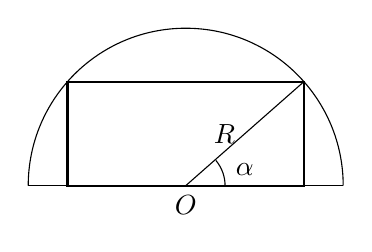
\begin{tikzpicture}
\draw (-2,0)--(2,0);
\draw (-2,0) arc (180:0:2);
\draw [thick] (-1.5,0) rectangle (1.5,1.32);
\draw (0,0)--node[left]{$R$}(1.5,1.32);
\node at (0,0)[below]{$O$};
\draw (.5,0) arc (0:40:.5);
\node at (.75,0)[above]{$\alpha$};

\end{tikzpicture}
    \caption{}
\end{figure}


\item 直角三角形的面积为12, 一锐角为$\beta$,求它的外接圆面
积,又当$\beta$是多少度时?外接圆面积最小。
\item 设 $\sin\alpha +\cos\alpha=\frac{1}{5}$,
求 $\sin2\alpha$, $\sin\alpha$, $\cos\alpha$, $\cos \frac{\alpha}{2}$, $\sin \frac{\alpha}{2}$。

\item \begin{enumerate}
    \item 已知$\cos\alpha =\frac{119}{169}$,求$\sin\frac{\alpha}{2}$, $\cos\frac{\alpha}{2}$和$\tan\frac{\alpha}{2}$。
    \item 已知$\cos\phi=\frac{1}{3}$,且$\phi\in(270^{\circ}, 360^{\circ})$,求$\sin\frac{\phi}{2}$, $\cos\frac{\phi}{2}$及$\tan\frac{\phi}{2}$。
\end{enumerate}
\item 已知$\cos\alpha=\frac{4}{5}$,且$\frac{3\pi}{2}<\alpha<2\pi$,求$\tan\frac{\alpha}{2}$。
\item 已知,等腰三角形顶角的余弦等于$\frac{7}{25}$, 求底角的正弦、
余弦和正切。
\item \begin{enumerate}
    \item 已知$\tan\alpha=\frac{4}{5}$, $180^{\circ}<\alpha<270^{\circ}$。
求$\tan\frac{\alpha}{2}$, $\sin2\alpha$, $\cos2\alpha$, $\tan 2\alpha$。
\item 已知$2\sin x+3\cos x=2$, 
求$\sin x$ 和 $\cos x$的值。
\end{enumerate}

\item 求证:
\begin{enumerate}
    \item $\left(\sin\frac{x}{2}-\cos\frac{x}{2}\right)^2=1-\sin x$
    \item $\tan\alpha-\cot\alpha=-2\cot 2\alpha$
    \item $\tan\left(\alpha+\frac{\pi}{4}\right)+\tan\left(\alpha-\frac{\pi}{4}\right)=2\tan\alpha$
    \item $\sin\theta+\cos\theta=\frac{1+\sin2\theta}{\sin\theta+\cos\theta}$
    \item $\sin\alpha(1+\cos2\alpha)=\sin2\alpha\cdot \cos\alpha$
    \item $2\sin\left(\frac{\pi}{4}+x\right)\sin\left(\frac{\pi}{4}-x\right)=\cos2x$
    \item $\frac{1+\tan\alpha}{1-\tan\alpha}=\frac{1+\sin2\alpha}{\cos^2\alpha-\sin^2\alpha}$
    \item $\frac{1+\sin2\theta-\cos2\theta}{1+\sin2\theta+\cos2\theta}=\tan\theta$
    \item $\frac{2\sin x-\sin2x}{2\sin x+\sin2x}=\tan^2\frac{x}{2}$
    \item $\frac{\tan\frac{\alpha}{2}}{1+\tan\frac{\alpha}{2}}+\frac{\tan\frac{\alpha}{2}}{1-\tan\frac{\alpha}{2}}=\tan\alpha$
\end{enumerate}

\item 利用$45^{\circ}$, $30^{\circ}$的三角函数值,求$\cos22^{\circ}30'$; $\sin22^{\circ}30'$; $\cos15^{\circ}$, $\sin15^{\circ}$的值。
\item \begin{enumerate}
    \item 求$\sin18^{\circ}$的值;
    \item 求证$\cos36^{\circ}-\cos72^{\circ}=\frac{1}{2}$。
\end{enumerate}

\item 求证:
\begin{enumerate}
    \item $\sin\frac{\pi}{8}=\frac{1}{2}\sqrt{2-\sqrt{2}}$
    \item $\tan 67.5^{\circ}=\sqrt{2}+1$
    \item $\tan 7^{\circ}30'=\sqrt{6}-\sqrt{3}+\sqrt{2}-2$
\end{enumerate}
\item 证明下列恒等式
\begin{enumerate}
    \item $2\sin\theta+\sin2\theta=4\sin\theta\cdot \cos^2\frac{\theta}{2}$
    \item $\tan 15^{\circ}+\cot 15^{\circ}=4$
    \item $\cos^2\alpha-2=\cos2\alpha\cdot \csc^2\alpha$
    \item $\sin(n\pi+x)\cos(n\pi-x)=\frac{1}{2}\sin 2x,\quad (n\in \mathbb{Z})$
    \item $\cos\alpha(\cos\alpha-\cos\beta)+\sin\alpha(\sin\alpha-\sin\beta)=2\sin^2\frac{\alpha-\beta}{2}$
    \item $\frac{\cos\alpha}{\sec\frac{\alpha}{2}+\csc\frac{\alpha}{2}}=\frac{1}{2}\left(\cos\frac{\alpha}{2}-\sin\frac{\alpha}{2}\right)$
    \item $\cos^4\theta=\frac{1}{4}+\frac{1}{2}\cos2\theta+\frac{1}{4}\cos^2 2\theta$
    \item $\sin^4\theta=\frac{3}{8}-\frac{1}{2}\cos2\theta+\frac{1}{8}\cos4\theta$
\end{enumerate}

\item 求证下列条件等式:
\begin{enumerate}
    \item 若$\tan x=\frac{b}{a}$,则$a\cos 2x+b\sin 2x=a$
    \item 若$\tan\alpha\frac{\alpha}{2}=\frac{m}{n}$,则$\sin\alpha+\frac{m}{n}\cos\alpha=1$
    \item 若$1+2\tan^2 x=\tan^2 y$,则$\sin^2x+\cos 2y=0$
    \item 若$x+y=3-\cos4\alpha$, $x-y=4\sin2\alpha$,则$x^{\tfrac{1}{2}}+y^{\tfrac{1}{2}}=2$
    \item 若$2\alpha+\beta=\frac{\pi}{2}$,则
    \[\sin\alpha=\sqrt{\frac{1-\sin\beta}{2}},\qquad \cos\alpha=\sqrt{\frac{1+\sin\beta}{2}}\]
\end{enumerate}
\end{enumerate}

\section{三角函数的和差化积与积化和差}
\subsection{三角函数的和差化积}

根据两角和差的正弦函数的定理有:
\[\begin{split}
    \sin(x+y)&=\sin x\cos y+\cos x\sin y\\
    \sin(x-y)&=\sin x\cos y-\cos x\sin y\\
\end{split}\]

由这两个等式左、右两端相加和相减得:
\begin{align}
 \sin (x+y) +\sin (x-y) &=2\sin x\cos y\\
\sin (x+y)-\sin (x-y) &=2\cos x\sin y   
\end{align}
设$x+y=\alpha$, $x-y=\beta$, 那么
\begin{equation}
    x=\frac{\alpha+\beta}{2},\qquad y=\frac{\alpha-\beta}{2}
\end{equation}

因此,上面两个等式(1.25)和(1.26)就变成
\begin{align*}
\sin\alpha+\sin\beta&=2\sin\frac{\alpha+\beta}{2}\cos\frac{\alpha-\beta}{2}\tag{I}\\
\sin\alpha-\sin\beta&=2\cos\frac{\alpha+\beta}{2}\sin\frac{\alpha-\beta}{2}\tag{II}
\end{align*}
根据两角和差的余弦函数的定理有:
\[\begin{split}
    \cos (x+y) &=\cos x\cos y - \sin x\sin y\\
\cos (x-y) &=\cos x\cos y +\sin x \sin y
\end{split}\]
由这两个等式左、右两端相加和相减得:
\begin{align}
    \cos (x+y) +\cos(x-y)&=2\cos x\cos y\\
\cos (x+y) -\cos (x-y) &=-2\sin x\sin y
\end{align}
以等式(1.27)代入上式得:
\begin{align*}
\cos\alpha+\cos\beta&=2\cos\frac{\alpha+\beta}{2}\cos\frac{\alpha-\beta}{2}\tag{III}\\
\cos\alpha-\cos\beta&=-2\sin\frac{\alpha+\beta}{2}\sin\frac{\alpha-\beta}{2}\tag{IV}
\end{align*}

利用上面得到的四个公式;即
\begin{blk}{和差化积公式}
\begin{align*}
    \sin\alpha+\sin\beta&=2\sin\frac{\alpha+\beta}{2}\cos\frac{\alpha-\beta}{2}\tag{I}\\
\sin\alpha-\sin\beta&=2\cos\frac{\alpha+\beta}{2}\sin\frac{\alpha-\beta}{2}\tag{II}\\
\cos\alpha+\cos\beta&=2\cos\frac{\alpha+\beta}{2}\cos\frac{\alpha-\beta}{2}\tag{III}\\
\cos\alpha-\cos\beta&=-2\sin\frac{\alpha+\beta}{2}\sin\frac{\alpha-\beta}{2}\tag{IV}
\end{align*}
\end{blk}

可以把某些三角函数的和或差化成积的形式。


\begin{example}
    把下列各式化成积的形式

\begin{tasks}(2)
    \task $1+\sin\alpha$
    \task $1-2\sin\alpha$
    \task $\sin\frac{\pi}{5}+\cos\frac{\pi}{5}$
    \task $\cos22^{\circ}-\sin 66^{\circ}$
\end{tasks}
\end{example}

\begin{solution}
\begin{enumerate}
    \item 方法1: 
\[\begin{split}
    1+\sin\alpha&=\sin90^{\circ}+\sin\alpha\\
    &=2\sin\frac{90^{\circ}+\alpha}{2}\cos\frac{90^{\circ}-\alpha}{2}\\
    &=2\sin\left(45^{\circ}+\frac{\alpha}{2}\right)\cos\left(45^{\circ}-\frac{\alpha}{2}\right)\\
    &=2\sin^2\left(45^{\circ}+\frac{\alpha}{2}\right)=2\cos^2\left(45^{\circ}-\frac{\alpha}{2}\right)
\end{split}\]

方法2: 
\[\begin{split}
    1+\sin\alpha &=1+\cos(90^{\circ}-\alpha)\\
    &=2\cos^2\left(45^{\circ}-\frac{\alpha}{2}\right)
\end{split}\]
\item \[\begin{split}
    1-2\sin\alpha &=2\left(\frac{1}{2}-\sin\alpha\right)\\
    &=2(\sin30^{\circ}-\sin\alpha)\\
    &=2\times 2\cos\frac{30^{\circ}+\alpha}{2}\sin\frac{30^{\circ}-\alpha}{2}\\
    &=4\cos\left(15^{\circ}+\frac{\alpha}{2}\right)\sin \left(15^{\circ}-\frac{\alpha}{2}\right)
\end{split}\]    
\item \[\begin{split}
    \sin\frac{\pi}{5}+\cos\frac{\pi}{5}&= \cos\left(\frac{\pi}{2}-\frac{\pi}{5}\right)+\cos\frac{\pi}{5}\\
    &=\cos\frac{3\pi}{10}+\cos\frac{\pi}{5}\\
    &=2\cos\frac{\frac{3\pi}{10}+\frac{2\pi}{10}}{2}\cos\frac{\frac{3\pi}{10}-\frac{2\pi}{10}}{2} \\
    &=2\cos\frac{\pi}{4}\cos\frac{\pi}{20}\\
    &=\sqrt{2}\cos\frac{\pi}{20}
\end{split}\]    
\item \[\begin{split}
    \cos22^{\circ}-\sin 66^{\circ}&=\cos22^{\circ}-\cos(90^{\circ}-66^{\circ}) \\
    &=\cos22^{\circ}-\cos 24^{\circ}\\
    &=-2\sin\frac{46^{\circ}}{2}\sin\left(-\frac{2^{\circ}}{2}\right)\\
    &=2\sin 23^{\circ}\sin 1^{\circ}
\end{split}\]    
\end{enumerate}
\end{solution}


\begin{example}
    把$\sin^2\alpha-\sin^2\beta$化为乘积形式。
\end{example}

\begin{solution}
方法1:
\[\begin{split}
    \sin^2\alpha-\sin^2\beta&=(\sin\alpha+\sin\beta)(\sin\alpha-\sin\beta)\\
    &=\left(2\sin\frac{\alpha+\beta}{2}\cos\frac{\alpha-\beta}{2}\right)\left(2\cos\frac{\alpha+\beta}{2}\sin\frac{\alpha-\beta}{2}\right)\\
    &=\left(2\sin\frac{\alpha+\beta}{2}\cos\frac{\alpha+\beta}{2}\right)\left(2\sin\frac{\alpha-\beta}{2}\cos\frac{\alpha-\beta}{2}\right)\\
    &=\sin(\alpha+\beta)\sin(\alpha-\beta)
\end{split}\]

方法2: 利用公式$\sin^2\alpha=\frac{1-\cos2\alpha}{2}$
进行替换,得到
\[\begin{split}
    \sin^2\alpha-\sin^2\beta&=\frac{1-\cos2\alpha}{2}-\frac{1-\cos2\beta}{2}\\
    &=\frac{1}{2}(\cos2\beta-\cos2\alpha)\\
    &=\frac{1}{2}\times (-2)\sin(\beta+\alpha)\sin(\beta-\alpha)\\
    &=\sin(\alpha+\beta)\sin(\alpha-\beta)
\end{split}\]
\end{solution}


\begin{example}
    引入辅助角把下面各式化为两角和的正弦函数。
\begin{enumerate}
    \item $3\cos\alpha+\sqrt{3}\sin\alpha$
    \item $3\cos\alpha-\sqrt{3}\sin\alpha$
    \item $\cos 2x-4\sin 2x$
\end{enumerate}
\end{example}

\begin{solution}
\begin{enumerate}
    \item \[\begin{split}
3\cos\alpha+\sqrt{3}\sin\alpha &=\sqrt{3}\left(\sqrt{3}\cos\alpha+\sin\alpha\right)\\
&=2\sqrt{3}\left(\frac{\sqrt{3}}{2}\cos\alpha+\frac{1}{2}\sin\alpha\right)\\
&=2\sqrt{3}\left(\sin60^{\circ}\cos\alpha+\cos60^{\circ}\sin\alpha\right)\\
&=2\sqrt{3}\sin(60^{\circ}+\alpha)=2\sqrt{3}\sin (\alpha+60^{\circ})        
    \end{split}\]

    \begin{figure}[htp]
        \centering
    \begin{tikzpicture}[>=latex]
\draw[->] (-2,0)--(2,0)node[right]{$x$};
\draw[->] (0,-2)--(0,2)node[right]{$y$};    
\draw[<->] (-1.1,0)--node[fill=white]{$\tfrac{\sqrt{3}}{2}$}(-1.1,1.3);
    \node at (.2,-.2){$O$};
\draw[thick] (0,0)--(120:1.5)--(-.75,0)node[below]{$-\tfrac{1}{2}$};
\draw[->] (.5,0) arc (0:120:.5);
\node at (60:.5)[right]{$120^{\circ}$};
\draw (120:1.5)--+(-.5,0);
\draw (0,0) circle(1.5) ; 
    \end{tikzpicture}
        \caption{}
    \end{figure}

    \item \[\begin{split}
 3\cos\alpha-\sqrt{3}\sin\alpha&=2\sqrt{3}\left(\frac{\sqrt{3}}{2}\cos\alpha-\frac{1}{2}\sin\alpha\right)\\       
 &=2\sqrt{3}\left(\sin120^{\circ}\cos\alpha+\cos120^{\circ}\sin\alpha\right)\\
 &=2\sqrt{3}\sin(120^{\circ}+\alpha)=2\sqrt{3}\sin (\alpha+120^{\circ})      
    \end{split}\]
    \item 配一个正系数$k$,使得
\[\cos 2x-4\sin 2x=k\left(\frac{1}{k}\cos2x-\frac{4}{k}\sin 2x\right)\]    
    并且引入一个辅助角$\theta$,满足下面两个等式:
\[\sin\theta=\frac{1}{k},\qquad \cos\theta=-\frac{4}{k}\]
$k$的值可由等式$\sin^2\theta+\cos^2\theta=\frac{1+(-4)^2}{k^2}=1$确定,于是有:
\[k=\sqrt{1+16}=\sqrt{17}\]
于是$\sin\theta=\frac{1}{\sqrt{17}}$, $\cos\theta=-\frac{4}{\sqrt{17}}$。$\theta$是第二象限角,它的值可由$\tan\theta=-\frac{1}{4}=-0.25$求出,得到
\[\theta=180^{\circ}-14^{\circ}2'=165^{\circ}58'\]
因此:
    \[\begin{split}
 \cos 2x-4\sin 2x&=\sqrt{17}\left(\sin165^{\circ}58'\cos 2x+\cos165^{\circ}58'\sin2x \right)       \\
 &=\sqrt{17}\sin (2x+165^{\circ}58')
    \end{split}\]
\end{enumerate}     
\end{solution}

\begin{example}
    化$a\sin x+b\cos x$为积的形式。
\end{example}

\begin{analyze}
仿照例1.29可以引入一个辅助角$\theta$, 并配上一个
正系数$k$, 我们来分析如何确定$k,\theta$:

假设$a=k\cdot \cos\theta$, $b=k\cdot\sin\theta$, 原式就变为
\[\begin{split}
    a\sin x+b\cos x&=k(\sin x\cdot \cos\theta+ \cos x\cdot \sin\theta)\\
    &=k\cdot \sin (x+\theta) 
\end{split}\]

由于$\sin^2\theta+\cos^2\theta=1$, 因而$\left(\frac{a}{k}\right)^2+\left(\frac{b}{k}\right)^2=1$
\[\therefore\quad k=\sqrt{a^2+b^2}\]
于是就得出
\[\cos\theta=\frac{a}{\sqrt{a^2+b^2}},\qquad  \sin\theta=\frac{b}{\sqrt{a^2+b^2}} \]
从而得
\[\tan\theta =\frac{b}{a}\]
这样,由$a,b$就可以确定$k,\theta$的值了。
\end{analyze}

\begin{solution}
\[a\sin x+b\cos x=\sqrt{a^2+b^2}\left(\frac{a}{\sqrt{a^2+b^2}}\sin x+\frac{b}{\sqrt{a^2+b^2}}\cos x\right)\]
令$\cos\theta=\frac{a}{\sqrt{a^2+b^2}},\quad  \sin\theta=\frac{b}{\sqrt{a^2+b^2}}$,则
\[\begin{split}
    \text{原式}&=\sqrt{a^2+b^2}(\cos\theta\cdot \sin x+\sin\theta \cdot \cos x)\\
&=\sqrt{a^2+b^2}\sin (x+\theta)
\end{split}\]
其中,$\theta$角所在的象限由$a,b$的符号确定,$\theta$角的值由
$\tan\theta=\frac{b}{a}$确定。
\end{solution}


\begin{example}
    若$A+B+C=180^{\circ}$, 求证
$\sin2A+\sin2B+\sin2C=4\sin A\sin B\sin C$
\end{example}

\begin{proof}
\begin{align*}
  &\quad   \sin2A+\sin2B+\sin2C\\
    &=2\sin (A+B) \cos(A-B) +2\sin C\cos C\\
    &=2\sin C\cos (A-B) +2\sin C\cos C \tag{$\sin (A+B)=\sin C$}\\
    &=2\sin C [\cos(A-B)+\cos C]\\
    &=2\sin C [\cos(A-B)-\cos(A+B)]
    \tag{$\cos C=-\cos (A+B)$}\\
    &=2\sin C [-2\sin A\sin (-B)]\\
    &=4\sin A\sin B\sin C  
\end{align*}
\end{proof}

\begin{rmk}
    在证明满足条件$A+B+C=180^{\circ}$ 的三个角$A$、$B$、$C$的三角函数恒等式时,要特别注意互为余角与互为补角的三角函数的性质,例如:    
从任何两个角的和是第三个角的补角这一类关系,得到
\[\sin (B+C) =\sin A,\qquad  \cos (A+B) = - \cos C,\qquad \tan (C+A) =-\tan B\]
\[\cos B= -\cos (C+A),\qquad \sin C=\sin (A+B) ,\qquad  \cot A=-\cot (B+C)\]

又从任何两个角的和的一半是第三个角的一半的余角这
一关系得到
\[\cos\frac{A+B}{2}=\sin\frac{C}{2},\qquad \sin\frac{C+A}{2}=\cos\frac{B}{2},\qquad \tan\frac{B+C}{2}=\cot\frac{A}{2}\]
\[\cos\frac{C}{2}=\sin\frac{A+B}{2},\qquad \sin\frac{A}{2}=\cos\frac{B+C}{2},\qquad \tan\frac{B}{2}=\cot\frac{C+A}{2}\]
\end{rmk}


\begin{example}
    把$1+\sin\theta+\cos\theta$化成积的形式。
\end{example}

\begin{solution}
\[\begin{split}
1+\sin\theta+\cos\theta&=(1+\cos\theta)+\sin\theta\\
&=2\cos^2\frac{\theta}{2}+2\sin\frac{\theta}{2}\cdot \cos\frac{\theta}{2}\\
&=2\cos\frac{\theta}{2}\left(\cos\frac{\theta}{2}+\sin\frac{\theta}{2}\right)\\
&=2\cos\frac{\theta}{2}\left[\sin\left(90^{\circ}-\frac{\theta}{2}\right)+\sin \frac{\theta}{2}\right]\\
&=2\cos\frac{\theta}{2}\cdot 2\sin 45^{\circ}\cdot \cos\left(45^{\circ}-\frac{\theta}{2}\right)\\
&=2\sqrt{2}\cos \frac{\theta}{2}\cdot \cos\left(45^{\circ}-\frac{\theta}{2}\right)
\end{split}\]
\end{solution}

\begin{ex}
\begin{enumerate}
    \item 把下列各式化为积的形式(口答)
\begin{tasks}(2)
    \task $\sin 24^{\circ}+\sin 20^{\circ}$
    \task $\sin 75^{\circ}-\sin 15^{\circ}$
    \task $\cos 3x+\cos 2x$
    \task $\cos\frac{\alpha+\beta}{2}-\cos\frac{\alpha-\beta}{2}$
\end{tasks}

\item 求值:
\begin{enumerate}
    \item $\frac{\sin20^{\circ}-\sin 40^{\circ}}{\cos 20^{\circ}-\sin 40^{\circ}}$
    \item $\sin 20^{\circ}+\sin 40^{\circ}-\sin 80^{\circ}$
\end{enumerate}

\item 求证:
\begin{enumerate}
    \item $\frac{\sin\alpha+\sin\beta}{\sin\alpha-\sin\beta}=\tan\frac{\alpha+\beta}{2}\cdot \cot\frac{\alpha-\beta}{2}$
    \item $\frac{\sin x+\sin y}{\cos x-\cos y}=\cot\frac{y-x}{2}$
    \item $\cos 2A+\cos 2B+\cos 2C=-1-4\cos A\cdot \cos B\cdot \cos C$,其中$A+B+C=\pi$
\end{enumerate}

\item 将下列各式化为两角和(差)的三角函数:
\begin{tasks}(2)
    \task $\frac{\sqrt{3}}{2}\sin x+\frac{1}{2}\sin x$
    \task $\frac{\sqrt{2}}{2}\cos x-\frac{\sqrt{2}}{2}\sin x$
    \task $\sqrt{2}\cos x+\sqrt{2}\sin x$
    \task $\cos\theta-\sqrt{3}\sin\theta$
    \task $4\sin\alpha+3\cos\alpha$
    \task $3\cos\beta-\sqrt{7}\sin\beta$
\end{tasks}
\end{enumerate}
\end{ex}

\subsection{三角函数的积化和差}
将公式(1.25)、(1.26)、(1.28)、(1.29)的两边同除以2,便得到如下公式:

\begin{blk}{积化和差公式}
\begin{align*}
\sin x\cdot\cos y  &= \frac{1}{2} [\sin (x+y) +\sin (x-y)] \tag{V}\\
\cos x\cdot \sin y &=\frac{1}{2}  [\sin (x+y)-\sin (x-y)] \tag{VI} 
\end{align*} 
\begin{align*}
\cos x\cdot\cos y  &= \frac{1}{2} [\cos (x+y) +\cos (x-y)] \tag{VII}\\
\cos x\cdot \sin y &=-\frac{1}{2}  [\cos (x+y)-\cos (x-y)]  \\
&=\frac{1}{2}[\cos (x-y)-\cos (x+y)] \tag{VIII}
\end{align*} 
\end{blk}

若$x=y$,由此可推出倍角公式,即有
\[\sin x\cos x=\frac{1}{2}\sin 2x,\qquad \cos^2 x=\frac{1}{2}(1+\cos 2x),\qquad \sin^2x=\frac{1}{2}(1-\cos2x)\]

\begin{example}
    化乘积$\sin35^{\circ} \cos55^{\circ}$ 为和的形式。
\end{example}

\begin{solution}
解法1: 
\[\sin35^{\circ} \cos55^{\circ} =\frac{1}{2}[\sin90^{\circ} +\sin (-20^{\circ} ) ]
=\frac{1}{2} [1-\sin20^{\circ} ]\]

解法2:
\[\sin35^{\circ} \cos55^{\circ}=\sin^2 35^{\circ} =\frac{1-\cos 70^{\circ}}{2}=\frac{1-\sin 20^{\circ}}{2}\]
\end{solution}


\begin{example}
    不查表,求下列各式的值:
\begin{enumerate}
    \item $\sin\frac{5\pi}{12}\cdot\cos\frac{\pi}{12}$
    \item $\cos^2 73^{\circ} +\cos^2 47^{\circ} +\cos73^{\circ} \cos47^{\circ}$
\end{enumerate}
\end{example}

\begin{solution}
\begin{enumerate}
    \item 解法1: 
\[\begin{split}
    \sin\frac{5\pi}{12}\cdot\cos\frac{\pi}{12}&=\frac{1}{2}\left[\sin\frac{\pi}{2}+\sin\frac{\pi}{3}\right]\\
    &=\frac{1}{2}+\frac{\sqrt{3}}{4}=\frac{1}{4}(2+\sqrt{3})
\end{split}\]    

解法2: 
\[\begin{split}
    \sin\frac{5\pi}{12}\cdot\cos\frac{\pi}{12}&=\cos\frac{\pi}{12}\cdot \cos\frac{\pi}{12}\\
    &=\cos^2\frac{\pi}{12}=\frac{1}{2}\left(1+\cos\frac{\pi}{6}\right)\\
    &=\frac{1}{2}\left(1+\frac{\sqrt{3}}{2}\right)=\frac{1}{4}\left(2+\sqrt{3}\right)
\end{split}\]    

\item \[\begin{split}
    \text{原式}&=1+\frac{\cos146^{\circ}}{2}+\frac{1+\cos94^{\circ}}{2}+\frac{\cos120^{\circ}+\cos26^{\circ}}{2}\\
    &=1+\frac{\cos146^{\circ}+\cos94^{\circ}}{2}-\frac{1}{4}+\frac{\cos26^{\circ}}{2}\\
    &=\frac{3}{4}+\frac{2\cos120^{\circ}\cos26^{\circ}}{2}+\frac{\cos26^{\circ}}{2}\\
    &=\frac{3}{4}-\frac{\cos26^{\circ}}{2}+\frac{\cos26^{\circ}}{2}\\
    &=\frac{3}{4}
\end{split}\]
\end{enumerate}
\end{solution}


\begin{example}
化简$\cos\alpha\cdot \cos2\alpha\cdot \cos4\alpha$并求$\cos\frac{\pi}{7}\cos\frac{2\pi}{7}\cos\frac{4\pi}{7}$的值。
\end{example}

\begin{solution}
\[\begin{split}
    \cos\alpha\cdot \cos2\alpha\cdot \cos4\alpha&=\frac{2\sin\alpha\cdot \cos\alpha\cdot \cos2\alpha\cdot \cos4\alpha}{2\sin\alpha}\\
    &=\frac{\sin2\alpha\cdot \cos2\alpha\cdot \cos4\alpha}{2\sin\alpha}\\
    &=\frac{\sin4\alpha\cdot \cos4\alpha}{2^2\sin\alpha}\\
    &=\frac{\sin8\alpha}{2^3\sin\alpha}=\frac{\sin 8\alpha}{8\sin \alpha}
\end{split}
\]
\[\cos\frac{\pi}{7}\cos\frac{2\pi}{7}\cos\frac{4\pi}{7}=\frac{\sin \frac{8\pi}{7}}{8\sin \frac{\pi}{7}}=\frac{-\sin\frac{\pi}{7}}{8\sin\frac{\pi}{7}}=-\frac{1}{8}\]
    
\end{solution}

\begin{example}
求证:
\begin{enumerate}
    \item $\sin15^{\circ} \cdot \sin30^{\circ} \cdot \sin75^{\circ} =\frac{1}{8}$
   \item  $\cos10^{\circ} \cdot \cos30^{\circ} \cdot \cos50^{\circ} \cdot \cos70^{\circ} =\frac{3}{16}$
\end{enumerate}    
\end{example}

\begin{proof}
\begin{enumerate}
    \item 证法1:
\[\begin{split}
\text{左边}&=\frac{1}{2}\sin 15^{\circ}\cdot \sin 75^{\circ}\\
&=-\frac{1}{4}[\cos 90^{\circ}-\cos(-60^{\circ})]\\
&=-\frac{1}{4}(0-\cos60^{\circ})\\
&=-\frac{1}{4}\left(-\frac{1}{2}\right)=\frac{1}{8}=\text{右边}    
\end{split}\]

证法2:
\[\begin{split}
\text{左边}&=\frac{1}{2}\sin 15^{\circ}\cdot \sin 75^{\circ}\\
&=\frac{1}{2}\sin 15^{\circ}\cdot \cos15^{\circ}\\
&=\frac{1}{4}\sin 30^{\circ}=\frac{1}{8}=\text{右边}    
\end{split}\]

\item 
\[\begin{split}
\text{左边}&=\cos 10^{\circ}\cdot \frac{\sqrt{3}}{2}\cdot \frac{1}{2}[\cos 120^{\circ}+\cos(-20^{\circ})]\\
&=\frac{\sqrt{3}}{4}\cos 10^{\circ}\left(-\frac{1}{2}+\cos20^{\circ}\right)\\ 
&=-\frac{\sqrt{3}}{8}\cos 10^{\circ}+\frac{\sqrt{3}}{4}\cos 10^{\circ}\cdot \cos 20^{\circ}\\
&=-\frac{\sqrt{3}}{8}\cos 10^{\circ}+\frac{\sqrt{3}}{8}[\cos30^{\circ}+\cos10^{\circ}]\\
&=-\frac{\sqrt{3}}{8}\cos 10^{\circ}+\frac{\sqrt{3}}{8}\cdot \frac{\sqrt{3}}{2}+\frac{\sqrt{3}}{8}\cos 10^{\circ}\\
&=\frac{3}{16}=\text{右边}
\end{split}\]
\end{enumerate}
\end{proof}

\begin{example}
求证:$\cos^3 2\alpha= \sin 3\alpha\cdot \sin^3\alpha+\cos 3\alpha\cdot \cos^3\alpha$
\end{example}

\begin{proof}
\[\begin{split}
\text{右边}&=\sin^2\alpha(\sin3\alpha\cdot \sin\alpha)+\cos^2\alpha(\cos3\alpha\cdot\cos\alpha)\\
&=\frac{1}{2}\big[\sin^2\alpha(\cos2\alpha-\cos4\alpha)+\cos^2\alpha(\cos4\alpha+\cos2\alpha)\big]\\
&=\frac{1}{2}\big[\cos 2\alpha(\sin^2\alpha+\cos^2\alpha)+\cos4\alpha(\cos^2\alpha-\sin^2\alpha)\big]\\
&=\frac{1}{2}\big[\cos2\alpha+\cos4\alpha\cdot\cos2\alpha\big]\\
&=\frac{1}{2}\cos2\alpha(1+\cos4\alpha)\\
&=\frac{1}{2}\cos2\alpha\cdot 2\cos^2 2\alpha\\
&=\cos^3 2\alpha=\text{左边}
\end{split}\]
\end{proof}

    

\begin{example}
    已知在$\triangle ABC$中,$\sin B\cdot \sin C=\cos^2\frac{A}{2}$。求证这个三角形是等腰三角形。
\end{example}


\begin{proof}
由于$\sin B\cdot \sin C=\cos\frac{A}{2}=\frac{1+\cos A}{2}$
且 $A=\pi-(B+C)$, $\cos A=-\cos(B+C)$, 因而就有
\[\sin B\cdot \sin C =\frac{1}{2} [1-\cos (B+C) ] \]
所以
\[-\frac{1}{2}[\cos (B+C) -\cos (B-C) ]
=\frac{1}{2}[1-\cos (B+C)]\]
化简上式,得$\cos (B-C) =1$。

又由$-180^{\circ}<B-C<180^{\circ}$,所以$B-C=0^{\circ}$,即$B=C$,这证明了$\triangle ABC$是等腰三角形。    
\end{proof}


\begin{example}
若$A+B+C=\pi$, 求证:
$$\cos\frac{A}{2}+\cos \frac{B}{2}+\cos \frac{C}{2}=4\cos\frac{\pi-A}{4}\cos\frac{\pi-B}{4}\cos\frac{\pi-C}{4}$$  
\end{example}

\begin{proof}
\[\begin{split}
&\quad  4\cos\frac{\pi-A}{4}\cos\frac{\pi-B}{4}\cos\frac{\pi-C}{4}\\
&= 2\cos\frac{\pi-A}{4}\left[\cos\frac{2\pi-(B+C)}{4}+\cos\frac{B-C}{4}\right]\\
&= 2\cos\frac{\pi-A}{4}  \cos\frac{\pi+A}{4} +2\cos\frac{\pi-A}{4} \cos\frac{B-C}{4} \\
&=\left(\cos\frac{\pi}{2}+\cos\frac{A}{2}\right)+2\cos\frac{B+C}{4}\cos\frac{B-C}{4}   \\
&=\cos\frac{A}{2}+\cos \frac{B}{2}+\cos \frac{C}{2}
\end{split}\] 
\end{proof}

\begin{ex}
\begin{enumerate}
    \item 先将各式化为和差形式,再查表求值:
\begin{tasks}(2)
    \task $2\sin70^{\circ}\cdot \cos20^{\circ}$
    \task $\cos80^{\circ}\cdot \sin120^{\circ}$
    \task $\cos68^{\circ}\cdot \cos52^{\circ}$
    \task $\sin121^{\circ}\cdot \sin50^{\circ}$
\end{tasks}          

    
    \item 不查表求值:
    \begin{enumerate}
        \item $\sin105^{\circ}\cdot \cos75^{\circ}$
        \item $2\cos37.5^{\circ}\cdot \cos22.5^{\circ}$
        \item $2\cos\frac{9\pi}{13}\cdot \cos\frac{\pi}{13}+\cos\frac{5\pi}{13}+\cos\frac{3\pi}{13}$
        \item $\sin^2 10^{\circ}+\cos^2 40^{\circ}+\sin 10^{\circ}\cdot \cos40^{\circ}$
    \end{enumerate} 
    
    \item 求证:
    \begin{enumerate}
        \item $2\sin\left(\frac{\pi}{3}+x\right)\cdot \cos\left(\frac{\pi}{3}-x\right)=\frac{\sqrt{3}}{2}+\sin 2x$
        \item $\sin20^{\circ}\cdot \cos70^{\circ}+\sin10^{\circ}\cdot \sin50^{\circ}=\frac{1}{4}$
        \item $\cos2\alpha\cdot \cos\alpha-\sin5\alpha\cdot \sin2\alpha=\cos4\alpha\cdot \cos3\alpha$
        \item $\cos4x\cdot \cos2x-\cos^2 3x=-\sin^2 x$
        \item $\tan\left(x+\frac{\pi}{4}\right)+\tan\left(x-\frac{\pi}{4}\right)=2\tan 2x$
    \end{enumerate} 
\end{enumerate}  
\end{ex}

\section*{习题1.3}
\addcontentsline{toc}{subsection}{习题1.3}
\begin{enumerate}
    \item 将函数的和化为乘积形式
    \begin{tasks}(2)
    \task $\sin 12^{\circ}+\sin 20^{\circ}$
    \task $\sin 40^{\circ}-\sin 16^{\circ}$
    \task $\cos 50^{\circ}+\cos 30^{\circ}$
    \task $\cos 17^{\circ}-\cos 13^{\circ} $
    \task $\sin 24^{\circ}+\cos 55^{\circ}$
    \task $\sin \frac{\pi}{5}-\cos \frac{2 \pi}{5}$
    \task $ \tan  10^{\circ}+\tan  20^{\circ}$
    \task $ \tan  12^{\circ}-\cot   40^{\circ}$
    \task $ \tan  \alpha+\cot   \alpha$ 
    \task $\cos \alpha-\sin \alpha$  
    \end{tasks}   
    \item 化函数的和式为乘积
\begin{tasks}(2)
\task  $\cos ^{2} \alpha-\cos ^{2} \beta$
\task  $\tan ^{2} \alpha-\tan ^{2} \beta$
\task  $1+\sin \alpha+\cos \alpha$
\task  $\sin 16^{\circ}+\sin 24^{\circ}+\sin 40^{\circ}$
\task     $\sin \alpha+\sin 2 \alpha+\sin 3 \alpha$
\task $\sin ^{2} x-\sin ^{2} y$   
\end{tasks}

    \item 化简下面式子
    \begin{enumerate}
    \item  $I \sin \omega t+I \sin \left(\omega t+\frac{2 \pi}{3}\right)+I \sin \left(\omega t-\frac{2 \pi}{3}\right)$
    \item  $ \cos ^{2} 3+\cos ^{2} 1-\cos 4 \cdot \cos 2$
    \item  $\sec \left(\frac{\pi}{4}+\alpha\right) \cdot \sec \left(\frac{\pi}{4}-\alpha\right)$
    \item  $\frac{\tan \left(45^{\circ}+x\right)-\tan \left(45^{\circ}-x\right)}{\tan \left(45^{\circ}+x\right)+\tan \left(45^{\circ}-x\right)}$
    \item  $\frac{\sin \alpha+\sin 3 \alpha+\sin 5 \alpha}{\cos \alpha+\cos 3 \alpha+\cos 5 \alpha}$   
    \end{enumerate}

    \item 引入辅助角将下面式子化为乘积形式:
\begin{tasks}(2)
\task $1+\sin \alpha$
\task $\frac{\sqrt{3}}{2}-\sin \alpha$
\task $\frac{\sqrt{2}}{2}+\cos \alpha$
\task $\frac{3}{4}-\sin ^{2} \alpha$
\task $\frac{1}{4}-\cos ^{2} \alpha$
\task $3-\tan^{2} \alpha$
\task $\sqrt{3}+2 \cos \alpha$
\task $\frac{\sqrt{3}}{2} \sin x-\frac{1}{2} \cos x$
\task $4 \sin x-3 \cos x$
\task $7 \sin 2 t-6 \cos 2 t$
\end{tasks}

\item 不查表,计算下面各式的值
\begin{tasks}(2)
\task $\sin 52^{\circ} 30' \cos 7^{\circ} 30'$
\task $\cos 97^{\circ} 30' \sin 37^{\circ} 30'$
\task  $2 \cos 165^{\circ} \cos 135^{\circ}$
\task  $\tan 10^{\circ} \cdot \tan 50^{\circ} \cdot \tan 70^{\circ} $
\task  $\cos 20^{\circ} \cos 40^{\circ} \cos 60^{\circ} \cos 90^{\circ}$
\task  $\cos 20^{\circ}+\cos 100^{\circ}+\cos 140^{\circ}$
\task  $\sin 20^{\circ} \sin 40^{\circ} \sin 60^{\circ} \sin 80^{\circ}$
\task  $\cos 40^{\circ} \cdot \cos 80^{\circ} \cdot \cos 160^{\circ}+\cos 160^{\circ} \cdot \cos 40^{\circ}$  
\end{tasks}

\item 化简下列各式
\begin{enumerate}
\item $2 \sin 2 \alpha \sin \alpha+\cos 3 \alpha$
\item $2 \cos \frac{9 \pi}{13} \cos \frac{\pi}{13}+\cos \frac{5 \pi}{13}+\cos \frac{3 \pi}{13}$
\end{enumerate}


\item 证明下列各等式:
\begin{enumerate}
\item $\frac{\sin A+\sin 3 A+\sin 5 A}{\sin 3 A+\sin 5 A+\sin 7 A}=\frac{\sin 3 A}{\sin 5 A}$
\item $\frac{\sin x-\sin y}{\sin (x+y)}=\frac{\sin \frac{1}{2}(x-y)}{\sin \frac{1}{2}(x+y)}$
\item $\frac{\cos(\alpha-\beta)}{\cos(\alpha+\beta)}=\frac{\cos2\alpha+\cos2\beta}{1+\cos 2(\alpha+\beta)}$
\item $\sin\frac{\alpha}{2}\cdot \sin\frac{7\alpha}{2}+\sin\frac{3\alpha}{2}\cdot\sin\frac{11\alpha}{2}=\sin2\alpha\cdot \sin 5\alpha$
\item $(\sin x+\cos x)(\sin 2x+\cos 2x)=\sin3x+\cos x$
\end{enumerate}

\item 若$A+B+C=\pi$,求证:
\begin{enumerate}
    \item $\cos A+\cos B+\cos C=1+4\sin\frac{A}{2}\sin\frac{B}{2}\sin\frac{C}{2}$
    \item $\sin^2\frac{A}{2}+\sin^2\frac{B}{2}+\sin^2\frac{C}{2}=1-2\sin\frac{A}{2}\sin\frac{B}{2}\sin\frac{C}{2}$
    \item $\tan A+\tan B+\tan C=\tan A\tan B\tan C$
    \item $\tan\frac{A}{2}\tan\frac{B}{2}+\tan\frac{B}{2}\tan\frac{C}{2}+\tan\frac{C}{2}\tan\frac{A}{2}=1$
\end{enumerate}

\item 若一三角形的边和角适合条件:
\[(a^2+b^2) \sin(A-B) =(a^2-b^2)\sin(A+B)\]
试证:此三角形为直角三角形或等腰三角形。

提示:用正弦定理$\frac{a}{\sin A}=\frac{b}{\sin B}=\frac{c}{\sin C}=2R$
\item 若$A$、$B$、$C$、$D$均在0与$\pi$之间,
求证:
\begin{enumerate}
    \item $\sin\frac{A+B}{2}\ge \frac{1}{2}(\sin A+\sin B)$
    \item $\sin\frac{A+B+C+D}{4}\ge \frac{1}{4}(\sin A+\sin B+\sin C+\sin D)$
    \item $\sin\frac{A+B+C}{3}\ge \frac{1}{3}(\sin A+\sin B+\sin C)$
\end{enumerate}
提示:在(b)中令$D=\frac{A+B+C}{3}$推导出(c)。

\item 求下列各式的最大值与最小值:
\begin{tasks}(2)
    \task $\sin x\cdot \cos x$
    \task $\sin\left(\alpha+\frac{\pi}{4}\right)+\sin\left(\alpha-\frac{\pi}{4}\right)$
    \task $\cos\left(\frac{\pi}{3}+2\theta\right)\sin\left(\frac{\pi}{3}-2\theta\right)$
    \task $6\cos x+8\sin x$
\end{tasks}
\end{enumerate}

\section{简单三角方程}
在初中我们曾经学习过这样的问题:已知三角函数值求角。如,已知$\sin x=\frac{1}{2}$, 求$x$的值,像这样条件等式$\sin x=\frac{1}{2}$的样子,我们把\textbf{含有未知数的三角函数的等式,叫做三角方程}。例如:$\sin x-1=-\frac{1}{2}$, 
$2\sin^2x+3\cos x=0$, $\sin5x=\cos4x$, 等等
都是三角方程。

解三角方程就是求出未知数的一切能适合下方程的值,或证明方程无解。

三角方程的一般理论和解法,留待以后学习,本节仅就几种特殊类型的简单三角方程的具体解法加以讨论。

\subsection{最简单的三角方程}

三角方程中,$\sin x=a$,
$\cos x=a$, $\tan x=a$, $\cot x=a$就叫做最简单的三角方程。它们的求解是其它三角方程求解的基础。

最简单的三角方程求解的方法是相同的,正像在初中已经学过的那样:首先求出,已知方程在$0\le x<2\pi$区间内的解,如果这个区间内有两个解:$x=\alpha_1$和$x=\alpha_2$, 那么原方程的所有解就是$x=\alpha_1+2k\pi$和$x=\alpha_2+2k\pi\quad (k\in\mathbb{Z})$; 如果在这个区间内只有一个解:$x=\alpha$, 那么原方程的解就是$x=\alpha+2k\pi$; 如果在这个区间没有解,那么原方程也没有解。可见,最简单的三角方程或有无限多解,或没有解。


\begin{example}
    解方程$\sin x=\frac{1}{2}$。
\end{example}

\begin{solution}
    已知在$(0, 2\pi)$内解为$x=\frac{\pi}{6}$和$x=\frac{5\pi}{6}$,
所以方程的解集为
\[\left\{x\Big|x=\frac{\pi}{6}+2k\pi\right\} \bigcup \left\{x\Big|x=\frac{5\pi}{6}+2k\pi\right\}\]
\end{solution}


\begin{example}
    解方程$\cos x=0$
\end{example}

\begin{solution}
    已知在$(0, 2\pi)$内,$x=\frac{\pi}{2}$和$x=\frac{3\pi}{2}$,所以方程的解为
    \[\begin{split}
 &\quad        \left\{x\Big|x=\frac{\pi}{2}+2k\pi\right\} \bigcup \left\{x\Big|x=\frac{3\pi}{2}+2k\pi=\frac{\pi}{2}(2k+1)\pi\right\}\\
        &=\left\{x\Big|x=\frac{\pi}{2}+2k\pi,\quad k\in\mathbb{Z}\right\} 
    \end{split} \]
\end{solution}


\begin{example}
    解方程$\sin x=-1$
\end{example}

\begin{solution}
    解集为$\left\{x\Big|x=\frac{3\pi}{2}+2k\pi,\quad k\in\mathbb{Z}\right\}$
\end{solution}

\begin{example}
    解方程$\cos x=2$
\end{example}

\begin{solution}
    由于任意角$\alpha$的余弦具有性质$|\cos\alpha|<1$, 因此,方程$\cos x=2$无解,即解集为$\emptyset$.
\end{solution}

\begin{example}
    解方程$\tan x=\frac{\sqrt{3}}{2}$
\end{example}

\begin{solution}
    由查表可知在$[0, 2\pi)$内,$x=40^{\circ}54'$和$x=220^{\circ}54'$。所以方程的解为
\[\begin{split}
   & \quad \left\{x\Big|x=40^{\circ}54'+k\cdot 360^{\circ}\right\} \cup \left\{x\Big|x=220^{\circ}54'+k\cdot 360^{\circ}\right\}\\
   &=\left\{x\Big|x=40^{\circ}54'+k\cdot 180^{\circ},\; k\in\mathbb{Z}\right\}
\end{split}\]
\end{solution}

一般地,可以概括出:
\begin{itemize}
    \item 方程 $\sin x=a$与$\cos x=a$, 当$|a|\le 1$时有解;当$|a|>1$时无解;
    \item 方程 $\tan x=a$与$\cot x=a$, 当$a$为任意实数时,都有解。
\end{itemize}

\begin{ex}
    解下列最简单三角方程
\begin{tasks}(2)
    \task $\sin x=-\frac{\sqrt{3}}{2}$
    \task $\sin x=0$
    \task $\cos x=-1$
    \task $\cos x=\frac{\sqrt{2}}{2}$
    \task $\tan x=0.5$
    \task $\cot x=-2.3016$
    \task $\sqrt{2}\sin x+1=0$
    \task $\tan x=2\sqrt{2}-1$
\end{tasks}
\end{ex}

\subsection{简单的三角方程}

有几类特殊而简单的三角方程,可以通过三角恒等变形或利用代数中解方程的方法,将它们化成一个或几个最简单的三角方程,从而求出它们的解集。

\begin{example}
    解方程
\begin{tasks}(2)
\tasks $2\cos2x=1$
\tasks $\tan (x+15^{\circ})+1=0$
\tasks $\sqrt{2}\sin(3x-9^{\circ})=\frac{\sqrt{2}}{2}$
\tasks $\cos^2x-4\cos x+2=0$
\end{tasks}
\end{example}

\begin{analyze}
  这几个三角方程的共同特点是:只含有同一个未知数的同名三角函数。因此可以将这个含有未知数的三角  
  函数视为一元,用代数方法先求出它的值,从而归结为最简单的三角方程求解。
\end{analyze}

\begin{solution}
 \begin{enumerate}
     \item 原方程化为 $\cos 2x=\frac{1}{2}$
\[2x=\pm\frac{\pi}{3}+2k\pi,\quad (k\in\mathbb{Z})\] 
所以解集是$\left\{x\Big|x=\pm\frac{\pi}{6}+k\pi,\quad k\in\mathbb{Z}\right\}$
\item  原方程化为$\tan(x+15^{\circ})=-1$
\[x+15^{\circ}=-45^{\circ}+k\cdot 180^{\circ},\quad (k\in\mathbb{Z})\]
所以解集是$\left\{x\Big|x=-60^{\circ}+k\cdot 180^{\circ},\quad k\in\mathbb{Z}\right\}$
\item 原方程化为 $\sin(3x-9^{\circ})=\frac{1}{2}$
\[3x-9^{\circ}=30^{\circ}+k\cdot 360^{\circ},\quad 3x-9^{\circ}=150^{\circ}+k\cdot 360^{\circ},\qquad (k\in\mathbb{Z})\]
所以解集为$$\left\{x\Big|x=13^{\circ}+k\cdot 120^{\circ},\quad k\in\mathbb{Z}\right\}\cup \left\{x\Big|x=53^{\circ}+k\cdot 120^{\circ},\quad k\in\mathbb{Z}\right\}$$
\item 原方程是关于$\cos x$的二次方程,解这个方程,得
\[\cos x=2+\sqrt{2},\qquad \cos x=2-\sqrt{2}\]
因为$2+\sqrt{2}>1$, 所以$\cos x=2+\sqrt{2}$无解;
从$\cos x=2-\sqrt{2}$, 可以解得:$x=\pm 54^{\circ}9'+k\cdot 360^{\circ}$, $(k\in\mathbb{Z})$。

所以原方程的解集是
$\left\{x\Big|x=\pm 54^{\circ}9'+k\cdot 360^{\circ},\quad k\in\mathbb{Z}\right\}$
 \end{enumerate}  
\end{solution}

\begin{example}
    解方程$2\sin^2x+3\cos x=0$。
\end{example}

\begin{analyze}
    利用三角公式,可以化为只含同一个未知数
的同名函数的三角方程求解。
\end{analyze}

\begin{solution}
    原方程化为$2(1-\cos^2x)+3\cos x=0$,即
\[2\cos^2x+3\cos x-2=0\]

解这个关于$\cos x$的二次方程,得
\begin{itemize}
    \item $\cos x=2$,它的解集为$\emptyset$;
    \item $\cos x=-\frac{1}{2},\quad x=\pm\frac{2\pi}{3}+2k\pi,\quad (k\in\mathbb{Z})$
\end{itemize}
所以原方程的解集是$\left\{x\Big|x=\pm \frac{2\pi}{3}+2k\pi,\quad k\in\mathbb{Z}\right\}$。
\end{solution}

\begin{example}
    解方程$\sin^2x-\frac{2\sqrt{3}}{3}\sin x\cdot \cos x-\cos^2x=0$。
\end{example}

\begin{analyze}
    方程的每一项中,关于$\sin x$与$\cos x$的次数
都相同(这里都是二次),我们叫做关于$\sin x$与$\cos x$的齐次方程,这种特点的方程可直接观察知道$\cos x=0$的$x$值,不会是方程的解、因此,这类方程可以两边同除以$\cos x$的某次幂而不会使方程增根或丢根的,这样就可以归结为含有未知数正切函数的方程求解了。
\end{analyze}

\begin{solution}
    原方程两边同除以$\cos^2x$得:$\tan^2x-\frac{2\sqrt{3}}{3}\tan x-1=0$

    解这个关于$\tan x$的二次方程,得
\begin{itemize}
    \item $\tan x=\sqrt{3},\qquad x=\frac{\pi}{3}+k\pi,\quad (k\in\mathbb{Z})$
    \item $\tan x=-\frac{\sqrt{3}}{3},\qquad x=-\frac{\pi}{6}+k\pi,\quad (k\in\mathbb{Z})$
\end{itemize}
所以原方程的解集是
\[\left\{x\Big|x=\frac{\pi}{3}+k\pi,\quad k\in\mathbb{Z} \right\}\bigcup \left\{x\Big| x=-\frac{\pi}{6}+k\pi,\quad k\in\mathbb{Z}\right\}\]

\end{solution}

\begin{example}
    解方程$\sin x=2\sin\left(\frac{\pi}{3}-x\right)$
\end{example}

\begin{solution}
    由和角公式$$\sin x=2\left(\sin\frac{\pi}{3}\cdot \cos x-\cos\frac{\pi}{3}\cdot \sin x\right)=\sqrt{3}\cos x-\sin x$$
所以 $2\sin x=\sqrt{3}\cos x$,两边同除以$2\cos x$,得
\[\tan x=\frac{\sqrt{3}}{2}\approx 0.8660\]
查表可得:$x=40^{\circ}54'+k\cdot 180^{\circ}\quad (k\in\mathbb{Z})$

所以原方程的解集是$\left\{x \Big|x=40^{\circ}54'+k\cdot 180^{\circ},\quad k\in\mathbb{Z}\right\}$
\end{solution}


\begin{example}
    解方程$\sqrt{3}\sin x=\frac{6}{\sqrt{3}}\cos^2\frac{x}{2}$
\end{example}

\begin{solution}
利用倍角公式变形
\[2\sqrt{3}\sin\frac{x}{2}\cdot \cos\frac{x}{2}-\frac{6}{\sqrt{3}}\cos^2\frac{x}{2}=0  \]
即:$\cos\frac{x}{2}\left(\sin\frac{x}{2}- \cos\frac{x}{2}\right)=0$

所以,原方程可分解为下面两个方程解
\[\cos\frac{x}{2}=0,\qquad \sin\frac{x}{2}-\cos\frac{x}{2}=0\]
\begin{itemize}
    \item 若$\cos\frac{x}{2}=0$,则$\frac{x}{2}=\pm\frac{\pi}{2}+2k\pi$,所以$x=\pm \pi+4k\pi,\quad (k\in\mathbb{Z})$
    \item 若$\sin\frac{x}{2}-\cos\frac{x}{2}=0$,可变形为$\tan\frac{\pi}{2}=1$,则$\frac{x}{2}=\frac{\pi}{4}+k\pi$,所以$x=\frac{\pi}{2}+2k\pi,\quad (k\in\mathbb{Z})$
\end{itemize}
因此原方程的解集是
\[\left\{x \Big|x=\pm \pi+4k\pi,\quad k\in\mathbb{Z}\right\}\bigcup \left\{x \Big|x=\frac{\pi}{2}+2k\pi,\quad k\in\mathbb{Z}\right\}\]
\end{solution}



\begin{ex}
解下列三角方程:
\begin{enumerate}
    \item $2\sin\frac{2x}{3}=1,\qquad 3\tan\frac{x+20^{\circ}}{3}=\sqrt{3}$
    \item $\sin^2x-2\sin x-3=0$
    \item $4\cos^2 x-4\sin x=1$
    \item \begin{enumerate}
        \item $2\sin x-5\cos x=0$
        \item $3\sin^2 x+2\sin x\cos x-5\cos^2 x=0$
    \end{enumerate}
    \item \begin{enumerate}
        \item $\sin\frac{x}{2}-\sqrt{3}\cos\frac{x}{4}=0$
        \item $4\cos\frac{x}{2}-5\cos x=5$
    \end{enumerate}
    \item \begin{enumerate}
        \item $\cos 3x+\cos 2x=0$
        \item $6\sin x+8\cos x=5$
    \end{enumerate}
\end{enumerate}
\end{ex}

\section*{习题1.4}
\addcontentsline{toc}{subsection}{习题1.4}
解下列三角方程:
    \begin{tasks}(2)
    \task $2\cos 2x=1$
    \task $\sin\left(\frac{x}{2}+\frac{\pi}{6}\right)=-\frac{\sqrt{3}}{2}$
    \task $2\cos\left(\frac{\pi}{3}+45^{\circ}\right)=1$
    \task $\tan2x-\sqrt{3}=0$
    \task $\frac{1}{2}\cot(x+25^{\circ})-2=0$
    \task $2\cos^2x-3\cos x+1=0$
    \task $\sin^2 2x=\sin 2x$
    \task $3\sin x-2\cos^2 x=0$
    \task $2\sin^2 x=1$
    \task $\sin^2 x-7\sin x\cdot \cos x+6\cos^2 x=0$
    \task $\sin x\cdot\cos x=\frac{1}{4}$
    \task $\sin 3x=\sin x$
    \task $3\sin^2 x-\sin 2x-\cos^2x=0$
    \task $\sin 2x=\cos 3x$
    \task $\sin\left(2x+\frac{\pi}{3}\right)+\sin\left(x-\frac{\pi}{6}\right)=0$
    \task $\sin\left(x+\frac{\pi}{6}\right)+\sin\left(x+\frac{\pi}{6}\right)=0$
    \task $5\cos2x+2\sin2x=0$
    \task $\cos^2x-3\sin^2 2x=0$
    \task $\sin\frac{x}{2}-\cos\frac{x}{2}=1$
    \task $4\sin x+3\cos x=3$
\end{tasks}

\section*{本章内容要点}
一、本章内容主要包括两角和、差、倍、半的三角函数
公式,以及三角函数的和差化积、积化和差的公式。这些公式的推导和变化,在数学和其它工程技术中都有广泛应用,要熟练地掌握。

二、掌握这些公式,主要应以两角和(差)的余弦公式为
基础,掌握和理解这些公式之间的内在联系和推导线索(见附表所列),这样可以帮助记忆。

三、除附表中所列主要公式外,还有
\begin{enumerate}
    \item 万能公式——用$\tan\frac{\alpha}{2}$
的有理式表示$\alpha$角的任何三角函
数。即
\[\sin\alpha=\frac{2\tan\frac{\alpha}{2}}{1+\tan^2\frac{\alpha}{2}},\quad \cos\alpha=\frac{1-\tan^2\frac{\alpha}{2}}{1+\tan^2\frac{\alpha}{2}},\quad \tan\alpha=\frac{2\tan\frac{\alpha}{2}}{1-\tan^2\frac{\alpha}{2}} \]

\item $a\sin x+b\cos x=\sqrt{a^2+b^2}\cdot \sin(x+\theta)$

其中,辅助角$\theta$由$a$、$b$的符号确定象限,由$\tan\theta=\frac{a}{b}$确定
数值。
\end{enumerate}

四、应用这些公式时,必须注意:凡使公式中某式子没有意义的角,都不适合公式;必须另加讨论。
在使用半角公式时,必须考察半角所在的象限,从而确定公式中根号前的符号。

五、本章还包括了简单三角方程及其解法的内容,主要是应用三角公式和代数方法解一些特殊类型的三角方程。其中有
\begin{enumerate}
    \item 最简单的三角方程
    \begin{itemize}
        \item $\sin x=a$, $\cos x=a$, 当$|a|\le 1$时有解;
        \item $\tan x=a$, $\cot x=a$, $a$为任意实数都有解。
    \end{itemize}

\item 简单三角方程,其中包括只含有一个未知数的同名
三角函数,关于$\sin x$及$\cos x$是齐次式、可变形为因式乘积的等特殊类型,一般都用解代数方程的方法,归结为解最简单的三角方程来求解。
\end{enumerate}

\section*{复习题一}
\addcontentsline{toc}{section}{复习题一}
\begin{enumerate}
    \item 求值:
\begin{enumerate}
    \item 已知$\cos2\alpha=\frac{3}{5}$,求$\sin^4\alpha-\cos^4\alpha$的值。
    \item 已知$\tan x=\frac{7}{24}$,求$\cos2x$, $\cot\left(2x-\frac{\pi}{4}\right)$的值。
    \item 已知$\sin\theta+\cos\theta=\frac{2}{3}$,求$\sin2\theta$的值。
    \item 已知$\sin\phi\cdot \cos\phi=\frac{60}{169}$,且$\frac{\pi}{4}<\phi<\frac{\pi}{2}$,求$\sin\phi$。
    \item 已知$\sin\alpha-\cos\alpha=m$, 求$\sin2\alpha$的值。
\end{enumerate}

\item 在$\triangle ABC$中
\begin{enumerate}
    \item 如果$\cos A=\frac{15}{17}$, $\cos B=\frac{9}{41}$,求$\cos C$;
    \item 如果$\tan A=2$, $\tan B=3$,求$\tan C$;
    \item 如果$\sin A=\frac{3}{5}$, $\cos B=\frac{5}{13}$,求$\cos C$;
    \item 如果$\sin A=\frac{4}{5}$, $\cos B=\frac{12}{13}$,求$\sin C$。
\end{enumerate}

\item \begin{enumerate}
    \item 等腰三角形底角的正弦为$\frac{13}{5}$,求顶角的正弦、余弦和正切;
    \item 等腰三角形顶角的余弦为$\frac{7}{25}$,求底角的正弦;
    \item 等腰三角形中,腰为底的2倍,求顶角的正弦、余弦。
\end{enumerate}

\item 证明下列各恒等式
\begin{enumerate}
    \item $\cos ^{4} A-\sin ^{4} A+1=2 \cos ^{2} A$
    \item $(\sin A+\cos A) \cdot(1-\sin A \cos A)=\sin ^{3} A+\cos ^{3} A$
    \item $\frac{1-\tan A}{1+\tan A}=\frac{\cot A-1}{\cot A+1}$
    \item $\frac{\cos A}{1-\tan A}+\frac{\sin A}{1-\cot A}=\sin A+\cos A$
    \item $\frac{\cot A \cos A}{\cot A+\cos A}=\frac{\cot A-\cos A}{\cot A \cos A}$
    \item $\frac{1+2 \sin A \cos A}{\sin ^{2} A-\cos ^{2} A}=\frac{\tan A+1}{\tan A-1}$
    \item $\frac{\cos A+\cos B}{\sin A-\sin B}+\frac{\sin A+\sin B}{\cos A-\cos B}=0$
    \item $\cot^{2} A-\cot^{2} B=\frac{\sin ^{2} B-\sin ^{2} A}{\sin ^{2} A \sin ^{2} B}$
\end{enumerate}

\item 求证:
\begin{enumerate}
    \item $2 \sin \left(\frac{\pi}{2}-\alpha\right) \sin (\pi-\alpha)=\sin 2 \alpha$
    \item $\left(\sin \frac{A}{2}-\cos \frac{A}{2}\right)^{2}=1-\sin A$
    \item $\cot \alpha-\tan \alpha=2 \cot 2 \alpha$
\item $\tan\left(x+\frac{\pi}{4}\right)+\tan\left(x-\frac{\pi}{4}\right)=2\tan 2x$
\item $1+\sin\alpha=2\cos^2\left(\frac{\pi}{4}-\frac{\alpha}{2}\right)$
\end{enumerate}

\item 把下列各式化为乘积的形式:
\begin{tasks}(2)
    \task $1+\sin 2A$
    \task $\frac{1}{2}-\cos x$
    \task $\frac{1}{2}\cos\alpha+\frac{\sqrt{3}}{2}\sin\alpha$
    \task $\sin\alpha-\cos\beta$
    \task $\sin^2\alpha-\sin2\beta$
    \task $\cos^2\alpha-\cos^2\beta$
    \task $\sin\alpha-\sin\beta+\sin(\alpha+\beta)$
    \task $1+\cos\theta+\cos\frac{\theta}{2}$
    \task $\sin\theta+\sin2\theta+\sin3\theta$
    \task $1-\frac{1}{4}\sin^2 2\alpha-\sin^2\beta-\cos^4\alpha$
\end{tasks}

\item \begin{enumerate}
    \item 当$\alpha$是多少度时,方程$2x^2+2\sqrt{2}x+\tan \alpha=0$有两个相等的实数根。($0^{\circ}\le \alpha\le 360^{\circ}$)
    \item $x^2-\cos\alpha x+\frac{1}{4}\sin2\alpha=0$, $\left(0<\alpha<\frac{\pi}{2}\right)$为
关于$x$的二次方程,当$\alpha$为何值时,方程有两个相等的实数根,它的根是什么?
\end{enumerate}
\item 若方程$5x^2-10x\cos \alpha+7\cos\alpha+6=0$的两根相等,试求两邻边之和为6, 且夹角为$\alpha$的平行四边形的最大面积。
\item 已知$A$、$B$是一个直角三角形的两个锐角,而且$\sin A$和
$\sin B$是方程$4x^2+kx+\sqrt{3}=0$的两个根,求$A$、$B$和$k$的值。
\item $\triangle ABC$的三个内角分别是$\alpha$、$\beta$、$\gamma$, 而$\tan \alpha$、$\tan \beta$是方程$x^2-5x+6=0$的两个根,求$\gamma$。
\item 确定$x$为何值时下列等式有意义
\[\sin x=\sqrt{1-\cos^2x},\qquad \cot\frac{x}{2}=\frac{\sin x}{1-\cos x}\]
\item 已知$0<\alpha<\frac{\pi}{2}$,求证$\sin\alpha+\cos\alpha>1$。
\item 已知$0<\alpha<\frac{\pi}{2}$,$0<\beta<\frac{\pi}{2}$,

问 $\sin(\alpha+\beta)$和$\sin\alpha+\sin\beta$哪个大?
\item 证明下列恒等式:
\begin{enumerate}
    \item $\tan 20^{\circ}+\tan 40^{\circ}+\sqrt{3}\tan 20^{\circ}\cdot \tan 40^{\circ}=\sqrt{3}$
    \item $\frac{\sin (2 x+y)}{\sin x}-2 \cos (x+y)=\frac{\sin y}{\sin x}$
    \item $\sec \theta=\sqrt{\frac{\sec ^{4} \theta-\tan ^{4}\theta}{2 \sin ^{2} \theta+\cos ^{2} \theta}}, \quad\left(0<\theta<\frac{\pi}{2}\right)$
    \item $\frac{3-4 \cos 2 A+\cos 4 A}{3+4 \cos 2 A+\cos 4 A}=\tan ^{4} A$
    \item $\frac{1+\cos A+\cos 2 A+\cos 3 A}{2 \cos ^{2} A+\cos A-1}=2 \cos A$
    \item $\tan  3 \theta-\tan  2 \theta-\tan  \theta=\tan  3 \theta \cdot \tan  2 \theta \cdot \tan  \theta$
    \item $\sin x+\sin y+\sin z-\sin (x+y+z)=4 \sin \frac{x+y}{2} \cdot \sin \frac{y+z}{2} \cdot \sin \frac{z+x}{2}$
    \item $\cos x+\cos y+\cos z+\cos (x+y+z)=4 \cos \frac{x+y}{2} \cdot \cos \frac{y+z}{2} \cdot \cos \frac{z+x}{2}$
\end{enumerate}


\item 在 $\triangle A B C$ 中, 求证:
\begin{enumerate}
    \item $\tan  A+\tan  B+\tan  C=\tan  A \cdot \tan  B \cdot \tan  C$
    \item $\frac{\cos A}{\sin B \cdot \sin C}+\frac{\cos B}{\sin A \cdot \sin C}+\frac{\cos C}{\sin A \cdot \sin B}=2$
    \item $\frac{\cos 2 A}{a^{2}}-\frac{\cos 2 B}{b^{2}}=\frac{1}{a^{2}}-\frac{1}{b^{2}}$
    \item $\left(a^{2}-b^{2}-c^{2}\right) \tan  A+\left(a^{2}-b^{2}+c^{2}\right) \tan  B=0$
\end{enumerate}


\item 在 $\triangle A B C$ 中, 证明:
\begin{enumerate}
    \item 若$\sin A=2\cos B\cdot \sin C$,则$\triangle A B C$为等腰三角形;
    \item 若$a^2=b(b+c)$,则$A=2B$;
    \item 若$\lg\sin A-\lg\cos B-\lg\sin C=\lg2$,则$\triangle A B C$是等腰三角形;
    \item 若$\sin C=\frac{\sin A+\sin B}{\cos A+\cos B}$,则$\triangle A B C$是直角三角形。
\end{enumerate}
\item 求下列函数的周期:
\begin{tasks}(2)
    \task $y=\frac{\sin x}{1+\cos x}$
    \task $y=2 \cos ^{2} \alpha-1$
    \task $y=4 \cos 2 \theta \sin ^{2} \theta$
    \task $y=\sqrt{3} \sin 2 \theta-\cos 2 \theta$
\end{tasks}    

\item 求函数$x=\tan\theta+\cot\theta$的极值,并求$\theta$为何值时达到这个极值。
\item 求下列函数的最大值与最小值
\begin{tasks}(2)
\task $y=\sin 3 x \cdot \cos 3 x$
\task $y=\sin \left(x-30^{\circ}\right) \cos x$
\task $y=\sin x-\sqrt{3} \cos x$
\task $y=\sin x+\cos x$
\task $y=a \sin x+b$
\task $y=\cos ^{4} x-\sin ^{4} x$
\end{tasks}    


\item 求函数$y=3\cos 2x+3\sqrt{3}\sin 2x-1$的振幅、周期、极大值和极小值。
\item 解下列三角方程:
 \begin{tasks}(2)
\task $4\sin ^{2} x+(2 \sqrt{3}-2) \cos x-(4-\sqrt{3})=0$
\task $\sec ^{2} x=1+\tan x$
\task  $\cos 2 x+\sin 3 x=0$
\task $\cos 3 x+2 \cos x=0$
\task $\tan 3 x=\tan 4 x$
\task $\frac{\sin 2 x}{\cos x}=\frac{\cos 2x}{\sin x}$
\task $5 \cos x+12 \sin x=13$
\task  $\sin 6 x \cdot \cos x=\sin 4 x \cdot \cos 3 x$
\task $\sin x \cdot \sin 7 x=\sin 3 x \cdot \sin 5 x$
\task $\sin 5x-\sin 3x=\sqrt{2}\cos 4x$
\end{tasks}   

\item 求证:
\begin{enumerate}
    \item 方程 $\sin^2x=\sin^2\alpha$的解集是$\{x|x=\pm \alpha+k\pi,\; k\in\mathbb{Z}\}$;
    \item 方程 $\tan^2x=\tan^2\alpha$的解集是$\{x|x=\pm \alpha+k\pi,\; k\in\mathbb{Z}\}$。
\end{enumerate}
\end{enumerate}
% \chapter{线性方程组}
在初中我们已经学习了二元一次,三元一次及一些四元一次方程组的概念与解法.一次方程也叫做线性方程,一次方程组也叫做线性方程组,它是代数学中最基本、应用最广泛的内容之一.本章将进一步研究线性方程组的消元法解的
程序,引进行列式及其性质,并应用行列式理论对线性方程的求解作一般性的讨论,从而对线性方程组的理论有较系统、完整的了解.

\section{高斯消元法}
我们已经知道,解线性方程组的基本思想是消元,而且已经掌握了代入消元法和加减消元法.但这两种消元法在应用中所采取的具体步骤和顺序,往往因人而异、因题而异,尤其是在解未知数较多的线性方程组时,计算程序很麻烦,消元的顺序又不只一个途径.这就启示我们,对于任一个线性方程组,如果能有比较统一的消元程序,在解的过程中就可以充分运用现代的电子计算机,提高解题效率,也便于人们在应用中掌握.因而就有高斯消元法.

\subsection{高斯消元法}
高斯消元法实质上也是加减消元法,
只是具有明确清晰的计算程序、统一的规格,便于掌握,便于使用电子计算机.

我们先从熟悉的例子分析起.

\begin{example}
    解方程组
\begin{numcases}{}
    3x+5y=11\\ 4x-3y=5
\end{numcases}
\end{example}

\begin{solution}
$(2.1)\x \frac{1}{3}$得
\begin{numcases}{}
    x+\frac{5}{3}y=\frac{11}{3} \\
    4x-3y=5 \tag{2.2}
\end{numcases}
$(2.2)-(2.3)\x 4$得
\begin{numcases}{}
    x+\frac{5}{3}y=\frac{11}{3}  \tag{2.3} \\
    -\frac{29}{3}y=-\frac{29}{3}  
\end{numcases}
$(2.4)\x \left(-\frac{3}{29}\right)$得
\begin{numcases}{}
    x+\frac{5}{3}y=\frac{11}{3}  \tag{2.3} \\
    y=1
\end{numcases}
(2.5)代入(2.3)得:
$\begin{cases}
    x=2\\y=1
\end{cases}$
所以原方程组的解集为$\{(x,y)\}=\{(2,1)\}$.
\end{solution}


\begin{example}
    解方程组
\begin{numcases}{}
3x+y-5z=18\\
x-3y+2z=3\\
5x-11y-8z=-13    
\end{numcases}
\end{example}

\begin{solution}
先将(2.6)、(2.7)互换,得
\begin{numcases}{}
x-3y+2z=3 \tag{2.7}\\
3x+y-5z=18\tag{2.6}\\
5x-11y-8z=-13  \tag{2.8}  
\end{numcases}
$(2.6)-(2.7)\x 3$且$(2.8)-(2.7)\x 5$,得
\begin{numcases}{}
    x-3y+2z=3 \tag{2.7}\\
    16y-11z=10 \\
    4y-18z=-28   
    \end{numcases}
$(2.10)\x\frac{1}{4}$后,再与(2.9)互换,得
\begin{numcases}{}
    x-3y+2z=3 \tag{2.7}\\
    y-\frac{9}{2} z=-7 \\
    16y-11z=10  \tag{2.9}  
    \end{numcases}
$(2.9)-(2.11)\x16$后,再乘以$\frac{1}{61}$,得
\begin{numcases}{}
    x-3y+2z=3 \tag{2.7}\\
    y-\frac{9}{2} z=-7 \tag{2.11}\\
    z=2
    \end{numcases}
(2.12)代入(2.11),再代入(2.7),整理可得:
\[\begin{cases}
    x=5\\y=2\\z=2
\end{cases}\]
所以原方程组的解集为$\{(x,y,z)\}=\{(5, 2, 2)\}$.
\end{solution}

通过以上两例可以知道,解线性方程组的消元法是可按一定顺序进行的.

第一步:将$x$的系数较小的方程换到第一个,并将$x$的系数
化为1, 消去后几个方程中的$x$; 再把第二个方程中$y$的系数化为1, 消去它后边几个方程中的$y$;……直到最后一个方程中最后一个未知数的系数化为1.

第二步:将最后一个未知数的值,分别回过头代入前边各方程中去,逐步可以得出方程组的解.

以三元线性方程组为例,上面两步消元求解的过程就是:
\[\begin{cases}
    a_1x+b_1y+c_1z=d_1\\
    a_2x+b_2y+c_2z=d_2\\
    a_3x+b_3y+c_3z=d_3\\
\end{cases}\mathop{\Longrightarrow}^{\text{第一步}} \begin{cases}
    x+b'_1y+c'_1z=d'_1\\
  \qquad \quad  y+c'_2z=d'_2\\
  \qquad \qquad \quad  z=d'_3
\end{cases}\mathop{\Longrightarrow}^{\text{第二步}}  \begin{cases}
    x=d_1''\\ y=d_2''\\ z=d_3'
\end{cases}\]

在这一过程中,就是反复将方程组施行了三种基本变换:
\begin{enumerate}
    \item 互换两个方程的位置;
    \item 用一个非零常数乘以一个方程两边;
    \item 用一个非零常数乘以一个方程后,加到另一个方程上.
\end{enumerate}

必须指出,变换方程组是为了消元求解,因此,变换前后的方程组应该有相同的解集(这时我们就说这两个方程组是同解的).那么,上述三种基本变换是否能保证方程组的同解性呢?我们肯定:经过上述三种基本变换,方程组的解集保持不变(同解的).

对于变换1、2, 结论显然是正确的;以下以三元一次
方程组为例来证明对于变换3, 结论是正确的,我们证明方程组
\begin{equation}
    \begin{cases}
      a_1x+b_1y+c_1z=d_1\\    a_2x+b_2y+c_2z=d_2\\    a_3x+b_3y+c_3z=d_3
    \end{cases}
\end{equation}
与
\begin{equation}
    \begin{cases}
        a_1x+b_1y+c_1z=d_1\\   (a_2+ka_1)x+(b_2+kb_1)y+(c_2+kc_1)z=d_2+kd_1\\
        a_3x+b_3y+c_3z=d_3
    \end{cases} 
\end{equation}
是同解的.

\begin{proof}
    设$(\alpha,\beta,\gamma)$是(2.13)的任一个解,则应有:
\[    \begin{cases}
    a_1\alpha+b_1\beta+c_1\gamma=d_1\\   
     a_2\alpha+b_2\beta+c_2\gamma=d_2\\    
    a_3\alpha+b_3\beta+c_3\gamma=d_3
  \end{cases}\]
把第一个等式的$k$倍加到第二等式上,得
\[    \begin{cases}
    a_1\alpha+b_1\beta+c_1\gamma=d_1\\  
     (a_2+ka_1)\alpha+(b_2+kb_1)\beta+(c_2+kc_1)\gamma=d_2+kd_1\\
    a_3\alpha+b_3\beta+c_3\gamma=d_3
\end{cases} \]
这说明$(\alpha,\beta,\gamma)$也是(2.14)的一个解.用类似的方法可以证明,方程组(2.14)的任一个解也是方程组(2.13)的解,因此(2.13)与(2.14)是同解的.
\end{proof}

注意,我们讨论的只是一般情形的消元过程,还有一些特殊的情形,我们将在以后系统讨论分析.这些特殊的情形在解题中都有可能出现,需要我们灵活处理.

\begin{example}
    解方程组
    \[\begin{cases}
     \qquad \;\; 3y+2z=5\\-x+2y-3z=2\\\;\; x+4y+7z=0 
    \end{cases}\]
\end{example}


\begin{solution}
运用例2.1、例2.2相同的高斯消元法,逐步将原方程组施以三种基本变换,可得
\[\begin{split}
\text{原方程组}& \Rightarrow \begin{cases}
  \quad   x+4y+7z=0\\-x+2y-3z=2\\\qquad \;\;3y+2z=5
\end{cases} \Rightarrow \begin{cases}
    x+4y+7z=0\\\qquad  6y+4z=2\\\qquad  3y+2z=5
\end{cases}\\
&\Rightarrow \begin{cases}
    x+4y+7z=0\\\qquad \;\; y+\frac{2}{3}z=\frac{1}{3}\\\qquad \;3y+2z=5 
\end{cases}\Rightarrow \begin{cases}
    x+4y+7z=0\\\qquad \;\;y+\frac{2}{3}z=\frac{1}{3}\\\qquad \;\;\qquad  0z=4
\end{cases}
\end{split}\]

到此就会发现,方程$0\cdot z=4$无解,亦无法回代其余方程,因此,原方程组无解,或说原方程组的解集为空集$\emptyset$.
\end{solution}
    
\begin{example}
    解方程组
    \[\begin{cases}
     \qquad \;\; 3y+2z=1\\-x+2y-3z=2\\\;\; x+4y+7z=0 
    \end{cases}\]
\end{example}

\begin{solution}
    \[\begin{split}
    \text{原方程组}& \Rightarrow \begin{cases}
      \quad   x+4y+7z=0\\-x+2y-3z=2\\\qquad \;\;3y+2z=1
    \end{cases} \Rightarrow \begin{cases}
        x+4y+7z=0\\\qquad  6y+4z=1\\\qquad  3y+2z=1
    \end{cases}\\
    &\Rightarrow \begin{cases}
        x+4y+7z=0\\\qquad \;\; y+\frac{2}{3}z=\frac{1}{3}\\\qquad \;3y+2z=1 
    \end{cases}\Rightarrow \begin{cases}
        x+4y+7z=0\\\qquad \;\;y+\frac{2}{3}z=\frac{1}{3}\\\qquad \qquad  0\cdot z=0
    \end{cases}
    \end{split}\]
    
    至此可知,方程$0\cdot z=0$有无限多个解($z$可取任意实数),设$z=t$, 回代各方程中,可以得出
    \[\begin{cases}
        x=-\frac{4}{3}-\frac{13}{3}t\\
        y=\frac{1}{3}-\frac{2}{3}t\\
        z=t
    \end{cases}\]
   所以原方程组有无限多个解,其解集为
    \[\{ (x,y, z) \} = \left\{ \left(-\frac{4}{3}-\frac{13}{3}t,\; \frac{1}{3}-\frac{2}{3}t,\; t\right) \right\}, \quad t\text{为任意数}\]
 \end{solution}
    
\begin{ex}
    用高斯消元法解下列线性方程组
\begin{multicols}{2}
    \begin{enumerate}
    \item $\begin{cases}
      \quad 5x-2y=8\\-7x+10y=4 
    \end{cases}$
    \item $\begin{cases}
        2x-3y+4z=8\\ 5x-y-8z=-21\\3x+5y-7z=-8
    \end{cases}$
    \item $\begin{cases}
      \qquad   y+2z=4\\x-3y\qquad =-8\\4x\quad\;\;\; -5z=7
    \end{cases}$
    \item $\begin{cases}
        7x-y+2z=1\\\qquad 5y-3z=0\\14x-2y+4z=1
    \end{cases}$
    \item $\begin{cases}
        3x-7y\qquad =2\\\qquad\quad  y-z=1\\12x-28y\quad =8
    \end{cases}$
\end{enumerate}    
\end{multicols}
\end{ex}
    
\subsection{一般二元一次方程组解的公式讨论}

利用高斯消元
法,我们对一般的二元一次方程组
\begin{numcases}{(\rm I)}
    a_1x+b_1y=c_1\\
    a_2x+b_2y=c_2
\end{numcases}
求解,并讨论它的各种情形.

在方程组(I)中,我们假定$a_1$与$b_1$, $a_2$与$b_2$, $a_1$与$a_2$,$b_1$与$b_2$分别不同时为零,因为,如若不然,不论上述哪一种
情形发生,方程组的解将是容易讨论的,同学们不妨试着自行讨论一下.

在这个假定下,利用高斯消元法(假定$a_1\ne 0$),可得
\begin{numcases}{}
x+\frac{b_1}{a_1}y=\frac{c_1}{a_1}\\
\frac{a_1b_2-a_2b_1}{a_1}y=\frac{a_1c_2-a_2c_1}{a_1}    
\end{numcases}
再将(2.18)变形后,可得
\begin{numcases}{}
    x+\frac{b_1}{a_1}y=\frac{c_1}{a_1} \tag{2.17}\\
    (a_1b_2-a_2b_1)y=a_1c_2-a_2c_1    
    \end{numcases}
由方程出发,可分别讨论如下:
\begin{enumerate}
    \item 当$a_1b_2-a_2b_1\ne 0$时,由(2.19)并代入(2.17)可以
得出方程组(I)唯一的一个解
\[\begin{cases}
    x=\frac{c_1b_2-c_2b_1}{a_1b_2-a_2b_1}   \\
    y=\frac{a_1c_2-a_2c_1 }{a_1b_2-a_2b_1}
\end{cases}\]
这就是原方程组的解的公式.

\item 当$a_1b_2-a_2b_1=0$时,由(2.19)又可以分为两种情形
讨论:
\begin{enumerate}
    \item 若$a_1c_2-a_2c_1\ne 0$,方程(2.19)变为一个矛盾方
程,共解集是空集,因而原方程组也就无解,其解集仍是空集.
\item 若$a_1c_2-a_2c_1=0$, 则方程(2.19)变为:$0y=0$, $y$可取任意实数$t$, 代入(2.17)得:
\[x=\frac{c_1}{a_1}-\frac{b_1}{a_1}t\]
这时方程组(I)有无限多解,解集为
\[\{(x,y)\}=\left\{\left(\frac{c_1-b_1t}{a_1}\right),\quad \text{$t$ 为任意实数}\right\}\]
\end{enumerate}
\end{enumerate}

\begin{blk}{定理}
方程组$\begin{cases}
    a_1x+b_1y=c_1\\
    a_2x+b_2y=c_2
\end{cases}$
其中$a_1$与$b_1$, $a_2$与$b_2$, $b_1$与$b_2$分别不同时为零.
\begin{enumerate}
    \item 当$a_1b_2-a_2b_1\ne 0$,它有唯一解;
    \[x=\frac{c_1b_2-c_2b_1}{a_1b_2-a_2b_1} ,\qquad 
    y=\frac{a_1c_2-a_2c_1 }{a_1b_2-a_2b_1}\]
    \item 当$a_1b_2-a_2b_1= 0$,且$a_1c_2-a_2c_1\ne 0$(或$c_1b_2-c_1b_1\ne 0$),它无解;
    \item 当$a_1b_2-a_2b_1= 0$,且$a_1c_2-a_2c_1= 0$,$c_1b_2-c_1b_1=0$,它有无限多个解.
\end{enumerate}
\end{blk}

\begin{example}
讨论方程组
\[\begin{cases}
    (a-b) x+ (a+b) y=2 (a^2-b^2)\\
    (a+b) x+ (a-b)y=2 (a^2+b^2)
\end{cases}\]
的解的情况.    
\end{example}

\begin{solution}
设$$a_1=a-b,\quad b_1 =a+b,\quad c_1=2 (a^2-b^2)$$
$$a_2=a+b,\quad b_2 =a-b,\quad c_2=2 (a^2+b^2)$$
则$$a_1b_2-a_2b_1=-4ab,\; a_1c_2-a_2c_1=-4ab(a-b),\; b_2c_1-b_1c_2=-4ab(a+b)$$所以
\begin{enumerate}
\item 若$a\ne 0$且$b\ne 0$, 则方程组有唯一解:
\[x=a+b,\qquad y=a-b\]
\item 若$a=0$或$b=0$, 则方程组有无限多个解.
\begin{enumerate}
    \item 在$a=0$, $b\ne 0$时,方程组的解集为:
\[\{(x,y)\}=\{(2b+t,t)|\text{$t$为任意数}\}\]
\item 在$a=0$, $b=0$时,方程组解集为
\[\{(x,y)\}=\{(2a-t,t)|\text{$t$为任意数}\}\]
\end{enumerate}

\item 若$a=b=0$, 则原方程组成为:
\[\begin{cases}
    0x+0y=0 \\ 0x+0y=0 
\end{cases}\]
显然两个方程组都是恒等式,$x,y$都可取任何数,因此方程组的解集是:
\[\{(x,y)\} =\{ (s,t)|\text{$s,t$为任意数}\}\]
\end{enumerate}
注意:本题不存在无解的情况.
\end{solution}

\begin{example}
有一个三位数,已知其十位数字等于其个位数字与百位数字之和,其个位数字与十位数字之和为$a$, 如果把三个数字的顺序倒过来,则所得新的三位数比原三位数大99. 求原三位数,并问参数$a$可取哪些值?
\end{example}


\begin{solution}
设原三位数的个位字为$x$, 百位数字为$y$, 由题目可知十位数字就是$a-x$. (其中$x,y$都是$1, 2,\ldots,9$这几个数字之一;$a-x$是$0, 1,\ldots,9$这十个数字之一).显然,$3\le a\le 18$. 依题意有:
\[\begin{cases}
    x+y=a-x\\
    100x+10(a-x)+y=100y+10(a-x)+x+99
\end{cases}\]
将上述方程组变换为:
\[\begin{cases}
    2x+y=a\\x-y=1
\end{cases}\]
由消元法可得出:$\begin{cases}
    x=\frac{1}{3}(a+1)\\ y=x-1
\end{cases}$
由上面这两个等式,不难断定:$a+1$须是3的倍数.所以,$a$只可能取$5, 8, 11, 14, 17$之中的一个值,直接计算可得:
\begin{itemize}
    \item $a=5$时,则$x=2$, $y=1$, $a-x=8$,
    可得出所求三位数为232;
\item $a=8$时,则$x=3$, $y=2$, $a-x=5$,
可得出所求三位数为253;
\item $a=11$时,则$x=4$, $y=8$, $a-x=7$,
可得出所求三位数为374;
\item $a=14$时,则$x=5$, $y=4$, $a-x=9$,
可得出所求三位数为495,
\item $a=17$时,虽可求出$x=6$, $y=5$, 但$a-x=11$已不符
合题意,因此,这种情形不可能出现.
 \end{itemize}   

所以,参数$a$分别取值5, 8, 11,与14,相应的三位数为:132, 253, 374, 495.
\end{solution}    

\begin{ex}
    试判别和讨论下列线性方程组的解的情形.
    \begin{multicols}{2}
\begin{enumerate}
    \item $\begin{cases}
        3x-5y=20\\6x-10y=15
    \end{cases}$
    \item $\begin{cases}
        3x-y=8\\2x+ay=7
    \end{cases}$
    \item $\begin{cases}
mx+y=m+1\\x+my=2m        
    \end{cases}$
\end{enumerate}        
    \end{multicols}
\end{ex}

\section*{习题2.1}
\addcontentsline{toc}{subsection}{习题2.1}

\begin{enumerate}
    \item 用高斯消元法解下列方程组:
\begin{multicols}{2}
\begin{enumerate}
    \item $\begin{cases}
        2x+8y-5z=3\\x-2y+z=0\\x+y+3z=7
    \end{cases}$
    \item $\begin{cases}
        x+y+2z=4\\2x-y+3z=4\\x+y+2z=3
    \end{cases}$
    \item $\begin{cases}
         x+2y-8z=5\\8x-2y+z=4\\-3x-6y+9z=15
    \end{cases}$
    \item $\begin{cases}
         x+2y-3z=5\\ -2x-4y+6z=-10\\ \frac{1}{2}x+y-\frac{3}{2}z=\frac{5}{2}
    \end{cases}$
    \item $\begin{cases}
        x_1+8x_2+5x_3+7x_4=12\\ 8x_1+5x_2+7x_3+x_4 =0\\
    5x_1+7x_2+x_3+3x_4=4\\ 7x_1+x_2+3x_3+5x_4=16
    \end{cases}$
    
\end{enumerate}    
\end{multicols}

    \item 讨论下列各方程组的解的情况:
\begin{multicols}{2}
\begin{enumerate}    
    \item $\begin{cases}
      x+y=12\\ x+ay=4  
    \end{cases}$
    \item $\begin{cases}
        6x-5y=25\\4x+ay=b
    \end{cases}$
    \item $\begin{cases}
        x=by\\px=qy
    \end{cases}$
    \item $\begin{cases}
        ax+by=a^2+2a+b^2\\
        bx+ay=a^2+2b+b^2
    \end{cases}$
\end{enumerate}    
\end{multicols}
    \item 一个两位数的两数字之和为 $a$, 若颠倒这两个数字的顺序,所得新的两位数比原数小36, 问$a$可能取那些值?原来的两位数是什么?
    \item 试判断$m$取何值时,下列方程组有唯一解:
\begin{enumerate}
    \item $\begin{cases}
        (m-1)x-(m+1)y=m+1\\ m^2x-(m+1)y=m-1
    \end{cases}$
    \item $\begin{cases}
x-(m^2-5)y=-1\\ (m+1)x -(m+1)^2y=1       
    \end{cases}$
\end{enumerate}

\item  高斯消元法对方程组的三种基本变换中,若把变换改为“用任一个常数乘一个方程.”删去“非零”二字行吗?为
什么?举例说明.
\end{enumerate}

\section{二阶行列式与二元线性方程组}
本节我们将从二元线性方程组的解的公式入手,引进二阶行列式的概念,从而学习二元线性方程组的行列式解法,并应用行列式讨论它的解的各种情形.

\subsection{二阶行列式}

一般的二元线性方程组
\begin{numcases}{(\text{I})}
    a_1x+b_1y=c_1\\
    a_2x+b_2y=c_2
\end{numcases}
当$a_1b_2-a_2b_1\ne 0$时,有唯一解,即
\begin{equation}
\begin{cases}
    x=\frac{c_1b_2-c_2b_1}{a_1b_2-a_2b_1}\\
    y=\frac{a_1c_2-a_2c_1}{a_1b_2-a_2b_1}
\end{cases}    
\end{equation}

分析公式(2.22)可以看出,两个分母都是$a_1b_2-a_2b_1$, 其中只含有未知数的系数.如果把方程组(I)中未知数的系数分离出来,按照它们原有的位置排列成一个正方形,即
\begin{center}\Large
    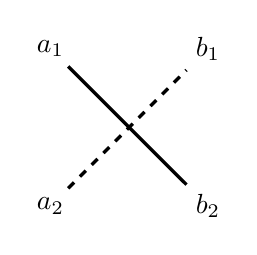
\begin{tikzpicture}
\node (A1) at (-1,1){$a_1$};
\node (A2) at (-1,-1){$a_2$};
\node (B1) at (1,1){$b_1$};
\node (B2) at (1,-1){$b_2$};
\draw [very thick](A1)--(B2);
\draw[dashed, very thick] (A2)--(B1);
    \end{tikzpicture}
\end{center}
那么可以看到$a_1b_2-a_2b_1$是这样两项的和:一项是正方形中实线所示的对角线(称为主对角线)上两个数的积,取正号;另一项是正方形中虚线所示的对角线(称为副对角线)上两个数的积,取负号.

为了便于记忆,我们将排正方形的四个数的两侧各加一
条竖直线,表示成
\[\begin{vmatrix}
    a_1&b_1\\a_2&b_2
\end{vmatrix}\]
并规定这个符号就是$a_1b_2-a_2b_1$即:
\begin{equation}
    \begin{vmatrix}
        a_1&b_1\\a_2&b_2
    \end{vmatrix}=a_1b_2-a_2b_1
\end{equation}

这时,(2.23)式的左边,就叫做二阶行列式;而(2.23)式的右边就是二阶行列式的展开式.

二阶列行式中,四个数称为它的元素;四个元素排成两
横排(称为行)两竖排(称为列),因而二阶行列共有二行二列.

所以,二阶行列式是一个值,它可按照(2.23)用对角线法则展开并计算出来.

\begin{example}
    展开并计算下列行列式:
\begin{multicols}{2}
\begin{enumerate}
    \item $\begin{vmatrix}
        2&3\\-5&-8
    \end{vmatrix}$
    \item $\begin{vmatrix}
        0&-7\\-3&10
    \end{vmatrix}$
    \item $\begin{vmatrix}
        m+1&m+2\\m&m+1
    \end{vmatrix}$
    \item $\begin{vmatrix}
        \sin x& \cos x\\ \cos x&\sin x
    \end{vmatrix}$
\end{enumerate}
\end{multicols}
\end{example}

\begin{solution}
由对角线法则可得,  
\begin{enumerate}
    \item $\begin{vmatrix}
        2&3\\-5&-8
    \end{vmatrix}=2\x(-8)-3\x (-5)=-1$
    \item $\begin{vmatrix}
        0&-7\\-3&10
    \end{vmatrix}=-21$
    \item $\begin{vmatrix}
        m+1&m+2\\m&m+1
    \end{vmatrix}=(m+1)^2-m(m+2)=1$
    \item $\begin{vmatrix}
        \sin x& \cos x\\ \cos x&\sin x
    \end{vmatrix}=\sin^2x-\cos^2x=-\cos2x$
\end{enumerate}
\end{solution}
  
\begin{ex}
\begin{enumerate}
    \item 展开并计算下列行列式的值:
\begin{multicols}{2}
\begin{enumerate}
    \item $\begin{vmatrix}
    8&4\\3&9
\end{vmatrix}$
    \item $\begin{vmatrix}
    a&a^2\\b&b^2
\end{vmatrix}$
\item $\begin{vmatrix}
    -3&21\\-1&7
\end{vmatrix}$
\item $\begin{vmatrix}
    6a-b&2b\\3a&b
\end{vmatrix}$
\item $\begin{vmatrix}
    \log_a x&\log_a x\\m&n
\end{vmatrix}$
\item $\begin{vmatrix}
    \sin x&\tan x\\ \cos x&\cot x
\end{vmatrix}$
\item $\begin{vmatrix}
     1-\sqrt{2}&2-\sqrt{3}\\2+\sqrt{3}&1+\sqrt{2}
\end{vmatrix}$
\item $\begin{vmatrix}
     x-1&x^3\\1&x^2+x+1
\end{vmatrix}$
\end{enumerate}
\end{multicols}

    \item 试试看,你能把下列各式分别用几个二阶行列式表示出来吗?
    \[am-bn,\qquad am+bn,\qquad a_1b_2-a_2b_1\]
    \item 求证:
    $\begin{vmatrix}
        a_1+ka_2 &b_1+kb_2 \\ a_2&b_2
    \end{vmatrix}=\begin{vmatrix}
        a_1  &b_1  \\ a_2&b_2
    \end{vmatrix}$
\end{enumerate}
\end{ex}

\subsection{二元线性方程组解的行列式表示及讨论}

在二元线性方程组的解的公式中,仔细观察可以发现,两分母,分子都可以很有规律地用行列式表示出来,即
\[\begin{split}
    a_1b_2-a_2b_1&=\begin{vmatrix}
        a_1&b_1\\a_2&b_2
    \end{vmatrix}\\
    c_1b_2-c_2b_1&=\begin{vmatrix}
        c_1&b_1\\c_2&b_2
    \end{vmatrix}\\
    a_1c_2-a_2c_1&=\begin{vmatrix}
        a_1&c_1\\a_2&c_2
    \end{vmatrix} 
\end{split}\]
这样,二元线性方程组解的公式就可以表示为:

当$\begin{vmatrix}
    a_1&b_1\\a_2&b_2
\end{vmatrix}\ne 0$时,
\[x=\frac{\begin{vmatrix}
    c_1&b_1\\c_2&b_2
\end{vmatrix}}{\begin{vmatrix}
    a_1&b_1\\a_2&b_2
\end{vmatrix}},\qquad y=\frac{\begin{vmatrix}
    a_1&c_1\\a_2&c_2
\end{vmatrix}}{\begin{vmatrix}
    a_1&b_1\\a_2&b_2
\end{vmatrix}}\]
为简便起见,通常把上述三个二阶行列式分别记为
\[D=\begin{vmatrix}
    a_1&b_1\\a_2&b_2
\end{vmatrix},\qquad D_x=\begin{vmatrix}
    c_1&b_1\\c_2&b_2
\end{vmatrix},\qquad D_y=\begin{vmatrix}
    a_1&c_1\\a_2&c_2
\end{vmatrix}\]
其中$D$ 的元素由方程组的未知数系数按顺序组成,就叫做这个方程组的系数行列式;$D_x$的元素由$D$将第一列元素($x$的系数)分别换成相应的常数项组成;$D_y$的元素由$D$将第二列元素($y$的系数)分别换成相应的常数项组成.

这样二元线性方程组(I)的解的公式,就可简化为:当$D\ne 0$时,
\[\begin{cases}
    x=\frac{D_x}{D}\\y=\frac{D_y}{D}
\end{cases}\]
即:二元线性方程组(I)的解集为
\[\{(x,y)\}=\left\{\left(\frac{D_x}{D},\; \frac{D_y}{D}\right)\right\}\]

\begin{example}
    用行列式法解方程组
    $\begin{cases}
11x-2y+5=0\\
8x+7y+24=0        
    \end{cases}$
\end{example}

\begin{solution}
    先将所给方程组写为一般形式
\[\begin{cases}
    11x-2y=-5\\
    8x+7y=-24
\end{cases}\]
再计算行列式$D$, $D_x$, $D_y$:
\[D=\begin{vmatrix}
    11&-2\\3&7
\end{vmatrix}=83\ne 0,\quad  D_x=\begin{vmatrix}
    -5&-2\\-24&7
\end{vmatrix}=-83,\quad  D_y=\begin{vmatrix}
    11&-5\\3&-24
\end{vmatrix}=-249\]
根据解的公式,得
\[x=\frac{D_x}{D}=-1,\qquad y=\frac{D_y}{D}=-3\]
所以,原方程组的解集为$\{(x,y)\}=\{(-1,-3)\}$.
\end{solution}

在使用行列式方法解二元线性方程组时,如果出现$D=0$时,解的公式不适用,这时可以仿照前文中对方程组解的讨论,得到以下结论:
\begin{itemize}
    \item 当$D=0$, 且$D_x\ne 0$(或$D_y\ne 0$)时,方程组的解集是空集$\emptyset$;
    \item 当$D=0$, 且$D_x=D_y=0$时,方程组有无限多个解,它的解集可引进一个参数表示.
\end{itemize}

注意,我们这里所指的二元线性方程组,限定其中的
$a_1$与$a_2$,$a_1$与$b_1$,$a_2$与$b_2$,$b_1$与$b_2$不同时为0.

\begin{example}
    用行列式法解下列方程组,并讨论:
    \[\begin{cases}
        mx+y-m-1=0\\
        x+my-2m=0   
    \end{cases}\]
   \end{example}
   
   
   
   \begin{solution}
先将原方程化为一般形式:
\[\begin{cases}
    mx+y=m+1\\
    x+my=2m   
\end{cases}\]
再计算各行列式:
\[\begin{split}
D&=\begin{vmatrix}
    m&1\\1&m
\end{vmatrix}=m^2-1=(m+1)(m-1)\\
D_x&=\begin{vmatrix}
    m+1&1\\2m&m
\end{vmatrix}=m(m+1)-2m=m(m-1)\\
D_y&=\begin{vmatrix}
    m&m+1\\1&2m
\end{vmatrix}=2m^2-(m+1)=(2m+1)(m-1)
\end{split}\]
所以
\begin{itemize}
    \item 当$m\ne -1$, $m\ne 1$时,$D\ne 0$方程组有唯一解,它的解集为
\[\{ (x,y) \} = \left\{ \left(\frac{m}{m+1},\frac{2m+1}{m+1}\right) \right\}\]
\item 当$m=-1$时,$D=0$, $D_x\ne 0$, 方程组无解,它的解集为$\emptyset$.
\item 当$m=1$时,$D=D_x=D_y=0$方程组有无限多个解,这时由于原方程组变为
$\begin{cases}
    x+y=2\\x+y=2
\end{cases}$
实际上就是$x+y=2$, 若令$x=t$, 则$y=2-t$, 因此,方程组的解集可表示为:
\[\{(x,y)\}=\{(t,2-t)|\text{$t$为任意数}\}\]
\end{itemize}

注意,在上述参数表示法中,可以有不同的表示法,如若令$y=a$, 则$x=2-a$, 解集就应表示为$\{(x,y)\}=\{(2-a,a)|\text{$a$为任意数}\}$.
\end{solution}

\begin{ex}
\begin{enumerate}
    \item 用行列式法解下列方程组
\begin{enumerate}
    \item $\begin{cases}
        x-8y=10\\6x-7y-11=0
    \end{cases}$
    \item $\begin{cases}
        14b-6y=-1\\ 3x+7y-6=0   
    \end{cases}$
    \item $\begin{cases}
        mx+ny=1\\nx+my=-1,\quad  (m\ne n) 
    \end{cases}$
    \item $\begin{cases}
        x\cos A-y\sin A=\cos B\\ x\sin A+y\cos A=\sin B
    \end{cases}$
\end{enumerate}

    \item 解下列方程组,并讨论
\begin{enumerate}
    \item $\begin{cases}
        x+ (m-1)y=1\\(m-1) x+y=2
    \end{cases}$
    \item $\begin{cases}
        mx+y=1\\ 4x+my-m=0
    \end{cases}$
    \item $\begin{cases}
        kx+ (2a-1) y=a^2+2a-1\\ x+ay=2a
    \end{cases}$
\end{enumerate}
\end{enumerate}   
\end{ex}

\section*{习题2.2}
\addcontentsline{toc}{subsection}{习题2.2}
\begin{enumerate}
    \item 计算下列行列式的值
\[\begin{vmatrix}
    \sqrt{6}&\sqrt{4}\\\sqrt{2}&\sqrt{3}
\end{vmatrix},\qquad \begin{vmatrix}
    \log_a b&4\\ 3& \log_b a
\end{vmatrix},\qquad\begin{vmatrix}
    e^{x+y}&e^x-1\\e^x+1&e^{x-y}
\end{vmatrix},\qquad\begin{vmatrix}
    1&1\\-\tan^2\alpha&1
\end{vmatrix}\]

\item 求证:
\begin{enumerate}
    \begin{multicols}{2}
    \item $\begin{vmatrix}
        a_1&b_1\\a_2&b_2
    \end{vmatrix}=\begin{vmatrix}
        a_1&a_2\\b_1&b_2
    \end{vmatrix}$
    \item $\begin{vmatrix}
        b_1 & b_2 \\a_1 &a_2
    \end{vmatrix}=-\begin{vmatrix}
        a_1&b_1\\a_2&b_2
    \end{vmatrix}$   
    \item $\begin{vmatrix}
        ka_1&kb_1\\b_1&a_2
    \end{vmatrix}=k\begin{vmatrix}
        a_1&b_1\\a_2&b_2
    \end{vmatrix}$
    \item $\begin{vmatrix}
        ka_1&\ell a_1\\ka_2& \ell a_2
    \end{vmatrix}=0$
\end{multicols}
    \item $\begin{vmatrix}
        a_1+a' &b_1+b'\\a_2&b_2
    \end{vmatrix}=\begin{vmatrix}
        a_1&b_1 \\a_2&b_2
    \end{vmatrix}+\begin{vmatrix}
        a'&b'\\ a_2&b_2
    \end{vmatrix}$
\end{enumerate} 

\item 用行列式解下列方程组:
\begin{multicols}{2}
\begin{enumerate}
    \item $\begin{cases}
        13x-7y-10=0\\19x+15y-2=0
    \end{cases}$
    \item $\begin{cases}
        \frac{7}{m}+\frac{9}{n}=3\\
        \frac{17}{m}+\frac{7}{n}=5
    \end{cases}$
\end{enumerate}
\end{multicols}
\item 解下列关于$x,y$的方程组,并讨论.
\begin{multicols}{2}
\begin{enumerate}
    \item $\begin{cases}
        mx+y=2m+1\\x-my=2-m
    \end{cases}$
    \item $\begin{cases}
        mx+y=-1\\8mx-my=2m+3
    \end{cases}$
    \item $\begin{cases}
        (a-1)x-(a^2-1)y=1\\
        (a^2-1)x+(a-1)y=2
    \end{cases}$
    \item $\begin{cases}
        kx+y=k+1\\
        x+ky=2k
    \end{cases}$
\end{enumerate}    
\end{multicols}

\item 当$k$为何值时,方程组$\begin{cases}
    4x+3y=1\\kx+(k-2)y=3
\end{cases}$的解中,$x$与$y$的值取异号?
\end{enumerate}

\section{三阶行列式与三元线性方程组}
\subsection{三阶行列式}

仿照二阶行列式,我们可以把九个数排成三行三列的正方形,并在两侧各加一竖直线.如
\begin{equation}
    \begin{vmatrix}
  a_1&b_1&c_1\\a_2&b_2&c_2\\a_3&b_3&c_3\\      
    \end{vmatrix}
\end{equation}
并规定它表示一个数
\begin{equation}
    a_1b_2c_3+a_2b_3c_1+a_3b_1c_2-a_3b_2c_1-a_2b_1c_3-a_1b_3c_2
\end{equation}

这时我们就把(2.24)叫做一个三阶行列式,(2.25)式就叫做这个三阶行列式的展开式(或这三阶行列式的值.)

三阶行列式共有九个元素,它的值也可以按下图所示
的对角线法则计算出来:
\begin{center}
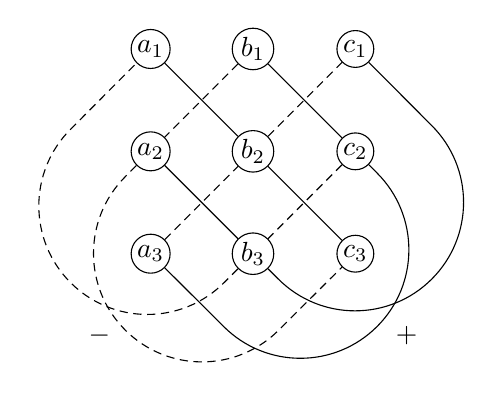
\begin{tikzpicture}[scale=1.3,inner sep=1pt]
    \draw(-1,1)node[shape=circle, draw](a1){$a_1$} (0,1)node[shape=circle, draw](b1){$b_1$} (1,1)node[shape=circle, draw](c1){$c_1$}
    (-1,0)node[shape=circle, draw](a2){$a_2$} (0,0)node[shape=circle, draw](b2){$b_2$} (1,0)node[shape=circle, draw](c2){$c_2$}
    (-1,-1)node[shape=circle, draw](a3){$a_3$} (0,-1)node[shape=circle, draw](b3){$b_3$} (1,-1)node[shape=circle, draw](c3){$c_3$};
\node at (-1.5,-1.8){$-$};
\node at (1.5,-1.8){$+$};
    \begin{scope}
    \draw(a1)--(b2)--(c3);
    \draw(b1)--(c2)--([turn]0:0.3)arc(45:-135:1.06)--(a3);
    \draw(a2)--(b3)--([turn]0:0.35)arc(-135:45:1.06)--(c1);
\end{scope}
    \begin{scope}[densely dashed]
        \draw(a3)--(b2)--(c1);
        \draw(c2)--(b3)--([turn]0:0.4)arc(-45:-225:1.06)--(a1);
        \draw(b1)--(a2)--([turn]0:0.35)arc(-225:-45:1.06)--(c3);
    \end{scope}
\end{tikzpicture}
\end{center}


实线所连三元素的乘积都取正号,共三项;虚线所连三元素乘积,都取负号,共三项.

\begin{example}
    用对角线法则计算下列三阶行列式:
\begin{multicols}{3}
\begin{enumerate}
    \item $\begin{vmatrix}
        1&3&5\\2&4&8\\3&0&-1
    \end{vmatrix}$
    \item $\begin{vmatrix}
        2&-3&1\\4&-1&7\\-1&5&2
    \end{vmatrix}$
    \item $\begin{vmatrix}
        x&y&z\\z&x&y\\y&z&x
    \end{vmatrix}$
\end{enumerate} 
\end{multicols}
\end{example}

\begin{solution}
由对角线法则可得:
\[\begin{split}
    \begin{vmatrix}
        1&3&5\\2&4&8\\3&0&-1
    \end{vmatrix}&=1\cdot 4\cdot (-1)+2\cdot 0\cdot 5+3\cdot 3\cdot8-3\cdot4\cdot5-2\cdot 3\cdot (-1)-1\cdot 0\cdot 8\\
    &=-4+0+77-60+6-0=14
\end{split}\]
\[\begin{split}
    \begin{vmatrix}
        2&-3&1\\4&-1&7\\-1&5&2
    \end{vmatrix}&=2\cdot(-1)\cdot2+4\cdot5\cdot1+(-1)\cdot(-3)\cdot7-(-1)\cdot(-1)\cdot1-4\cdot(-3)\cdot2-2\cdot5\cdot7\\
    &=-4+20+21-1+24-70=-10
\end{split}\]
\[\begin{vmatrix}
    x&y&z\\z&x&y\\y&z&x
\end{vmatrix}=x^3+y^3+z^3-3xyz\]
\end{solution}

\begin{ex}
\begin{enumerate}
\item 计算下列三阶行列式    
\[\begin{vmatrix}
    3&1&2\\1&0&0\\-1&0&0
\end{vmatrix},\quad \begin{vmatrix}
    1&a&a^2\\1&b&b^2\\1&c&c^2
\end{vmatrix},\quad \begin{vmatrix}
    0&a&b\\a&0&c\\b&c&0
\end{vmatrix},\quad \begin{vmatrix}
    1&a&b\\-a&1&c\\-b&-c&1
\end{vmatrix},\quad \begin{vmatrix}
    a&d&e\\0&b&d\\0&0&c
\end{vmatrix}\]

\item 先计算行列式的值,再比较结果找出各组中两行列式之间的关系:
\begin{enumerate}
    \item $\begin{vmatrix}
        1&4&7\\2&5&8\\3&6&9
    \end{vmatrix},\qquad \begin{vmatrix}
        1&2&3\\4&5&6\\7&8&9
    \end{vmatrix}$
    \item $\begin{vmatrix}
        a&1&2\\1&a&1\\2&1&a
    \end{vmatrix},\qquad \begin{vmatrix}
        ak&k&2k\\1&a&1\\2&1&a
    \end{vmatrix}$
\end{enumerate}
\end{enumerate}    
\end{ex}

\subsection{三阶行列式的性质}

为了简化行列式的计算,更好地掌握这一工具,我们进一步学习行列式的性质.

\begin{blk}{定理1 }
    如果把一个行列式的每一行(列),同时改为同号数的列(行),那么,所得的行列式与原行列式的值相等.
\[\Delta=\begin{vmatrix}
    a_1&b_1&c_1\\a_2&b_2&c_2\\a_3&b_3&c_3
\end{vmatrix}=\begin{vmatrix}
    a_1&a_2&a_3\\b_1&b_2&b_3\\c_1&c_2&c_3
\end{vmatrix}=\Delta'\]
\end{blk}

 \begin{proof}
由对角线法则知    
\[\begin{split}
    \Delta &=a_1b_2c_3+a_2b_3c_1+a_3b_1c_2-a_3b_2c_1-a_2b_1c_3-a_1b_3c_2\\
    \Delta'&=a_1b_2c_3+a_2b_3c_1+a_3b_1c_2-a_3b_2c_1-a_2b_1c_3-a_1b_3c_2\\
\end{split}\]
所以$\Delta=\Delta'$
 \end{proof}


 由定理1可知:对于行列式的行成立的性质对于列也一定成立;反过来,对于列成立的性质对于行也一定成立,所以今后关于行列式的性质,只需对行证明就行了.

\begin{blk}{定理2}
    如果把一个行列式的任意两行(列)对调,那么,所得的行列式与原行列式的绝对值相等,符号相反.
    \[\Delta=\begin{vmatrix}
        a_1&b_1&c_1\\a_2&b_2&c_2\\a_3&b_3&c_3
    \end{vmatrix}=-\begin{vmatrix}
        a_2&b_2&c_2\\a_1&b_1&c_1\\a_3&b_3&c_3
    \end{vmatrix}=-\Delta'\]
\end{blk} 

\begin{proof}
    只要以对调第一、二行为例证明结论,其它行(列)对调的证明是类似的.
    仍由三阶行列式的对角线法则可得
    \[\begin{split}
        \Delta&=a_1b_2c_3+a_2b_3c_1+a_3b_1c_2-a_3b_2c_1-a_2b_1c_3-a_1b_3c_2\\
        &=-(a_2b_1c_3+a_1b_3c_2+a_3b_2c_1-a_3b_1c_2-a_1b_2c_3-a_2b_3c_1)\\
        &=-\Delta'
    \end{split}\]
    所以$\Delta=-\Delta'$
\end{proof}

\begin{blk}{定理3}
 如果一个行列式中,有两行(列)元素完全对应相同,那么,这个行列式的值必须等于零.   
 \[\Delta=\begin{vmatrix}
     a_1&a_2&a_3\\ b_1&b_2&b_3\\a_1&a_2&a_3
 \end{vmatrix}=0\]
\end{blk}

\begin{proof}
只要将行列式中相同的两行(列)对调,则所得行列式仍为$-\Delta$, 但根据定理2又可知,对调后应得$-\Delta$.于是就有,    
\[\Delta=-\Delta\]
所以可得:$\Delta=0$.
\end{proof}

\begin{blk}{定理4}
如果把一个行列式的某一行(列)的所有元素同乘以任一数$k$, 那么,所得行列式的值就等于原行列式值的$k$倍.
\[\Delta'=\begin{vmatrix}
    a_1&b_1&c_1\\ka_2&kb_2&kc_2\\a_3&b_3&c_3
\end{vmatrix}=k\cdot \begin{vmatrix}
    a_1&b_1&c_1\\a_2&b_2&c_2\\a_3&b_3&c_3
\end{vmatrix}=k\Delta\]
\end{blk}

\begin{proof}
由对角线法则将它们展开、比较,就可直接证明结论$\Delta'=k\Delta$是正确的.
\end{proof}

\begin{blk}{定理5}
    如果在行列式中,某一行(列)各元素有公因子时,则可以把公因子提到行列式的外边.
\[\begin{vmatrix}
    ka_1&kb_1&kc_1\\a_2&b_2&c_2\\a_3&b_3&c_3
\end{vmatrix}=k\cdot \begin{vmatrix}
    a_1&b_1&c_1\\a_2&b_2&c_2\\a_3&b_3&c_3
\end{vmatrix}
    \]
\end{blk}

这定理的证明可由定理4直接得出,这里不再重述,但要指出,这个定理可以使行列式计算简化,在应用中很重要.例如,运用它可这样计算行列式:
\[\begin{split}
\begin{vmatrix}
    -\tfrac{1}{2}&-\tfrac{2}{3}&-1\\
    \tfrac{5}{2}&\tfrac{4}{3}&0\\
    \tfrac{9}{2}&\tfrac{7}{3}&1
\end{vmatrix}&=(-1)\x\frac{1}{2}\x\frac{1}{3}\x\begin{vmatrix}
    1&2&1\\5&4&0\\9&7&1
\end{vmatrix}\\
&=\left(-\frac{1}{6}\right)\x(-7)=1\frac{1}{6}
\end{split}\]

\begin{blk}{定理6}
    如果一个行列式中有一行(列)的元素全为零,则这个行列式的值等于零.
    \[\begin{vmatrix}
        0&0&0\\a_2&b_2&c_2\\a_3&b_3&c_3
    \end{vmatrix}=0\]
\end{blk}

\begin{proof}
    由定理5与零的运算特性可得
\[\begin{vmatrix}
    0&0&0\\a_2&b_2&c_2\\a_3&b_3&c_3
\end{vmatrix}=\begin{vmatrix}
    0\cdot a_1&0\cdot b_1&0\cdot c_1\\a_2&b_2&c_2\\a_3&b_3&c_3
\end{vmatrix}=0\cdot\begin{vmatrix}
    a_1&b_1&c_1\\a_2&b_2&c_2\\a_3&b_3&c_3
\end{vmatrix}=0\]
\end{proof}

\begin{blk}{定理7}
    如果一个行列式中有两行(或两列)的对应元素成比例,则这个行列式等于零.
\[\begin{vmatrix}
    ka_2&kb_2&kc_2\\a_2&b_2&c_2\\a_3&b_3&c_3
\end{vmatrix}=0\]
\end{blk}

\begin{proof}
    由定理5及定理8可以知道:
    \[\begin{vmatrix}
        ka_2&kb_2&kc_2\\a_2&b_2&c_2\\a_3&b_3&c_3
    \end{vmatrix}=k\cdot\begin{vmatrix}
        a_2&b_2&c_2\\a_2&b_2&c_2\\a_3&b_3&c_3
    \end{vmatrix}=k\cdot 0=0\]
\end{proof}

\begin{blk}{定理8}
如果行列式某一行(或一列)的元素都是二项式之和的形式,则这个行列式等于两个行列式之和.
\[\begin{vmatrix}
    a_1+a'_1&b_1+b'_1&c_1+c'_1\\a_2&b_2&c_2\\a_3&b_3&c_3
\end{vmatrix}=\begin{vmatrix}
    a_1&b_1&c_1\\a_2&b_2&c_2\\a_3&b_3&c_3
\end{vmatrix}+\begin{vmatrix}
    a'_1&b'_1&c'_1\\a_2&b_2&c_2\\a_3&b_3&c_3
\end{vmatrix}\]
\end{blk}

证明要点:用三阶行列式的对角线法则,将左边的行列式展开,再由乘法对加法的分配律、交换律即可证明其结果与右边两个行列式的和展开后的结果是一样的.同学们可以自证.

\begin{blk}{定理9}
    如果把行列式的某一行(列)所有的元素同乘以同一个数k后,加到另一行(列)的对应元素上,则所得行列式与原行列式是相等的.
\[\begin{vmatrix}
    a_1&b_1&c_1\\a_2+a_1k&b_2+b_1k&c_2+c_1k\\a_3&b_3&c_3
\end{vmatrix}=\begin{vmatrix}
    a_1&b_1&c_1\\a_2&b_2&c_2\\a_3&b_3&c_3
\end{vmatrix}\]
\end{blk}

\begin{proof}
    由定理8可得:
\[\begin{vmatrix}
    a_1&b_1&c_1\\a_2+a_1k&b_2+b_1k&c_2+c_1k\\a_3&b_3&c_3
\end{vmatrix}=\begin{vmatrix}
    a_1&b_1&c_1\\a_2&b_2&c_2\\a_3&b_3&c_3
\end{vmatrix}+\begin{vmatrix}
    a_1&b_1&c_1\\a_1k&b_1k&c_1k\\a_3&b_3&c_3
\end{vmatrix}\]
又由定理7可知:
\[\begin{vmatrix}
    a_1&b_1&c_1\\a_1k&b_1k&c_1k\\a_3&b_3&c_3
\end{vmatrix}=0\]
所以
\[\begin{vmatrix}
    a_1&b_1&c_1\\a_2+a_1k&b_2+b_1k&c_2+c_1k\\a_3&b_3&c_3
\end{vmatrix}=\begin{vmatrix}
    a_1&b_1&c_1\\a_2&b_2&c_2\\a_3&b_3&c_3
\end{vmatrix}\]
\end{proof}



有了行列式的这些性质,只要在计算中充分灵活地使用,就会很简捷地得到结果.

\begin{example}
    计算行列式$\Delta=\begin{vmatrix}
        234&3&4\\
        125&2&5\\
        476&7&6
    \end{vmatrix}$的值.
\end{example}

\begin{solution}
由定理8可知
\[\Delta=\begin{vmatrix}
    200&3&4\\
    100&2&5\\
    400&7&6
\end{vmatrix}+\begin{vmatrix}
    30&3&4\\
    20&2&5\\
    70&7&6
\end{vmatrix}+\begin{vmatrix}
    4&3&4\\
    5&2&5\\
    6&7&6
\end{vmatrix}\]
又由定理7与定理3可知,第二个行列式与第三个行列式的值均为零,而由定理5可知,第一个行列式的第一列各数的公因数100可提到行列式外边,所以,
\[\Delta=100\cdot \begin{vmatrix}
    2&3&4\\
    1&2&5\\
    4&7&6
\end{vmatrix}=100\cdot (-8)=-800\]
\end{solution}

\begin{example}
计算行列式$\Delta=\begin{vmatrix}
        a&a+1&a+2\\
        b&b+1&b+2\\
        c&c+1&c+2\\
    \end{vmatrix}$的值.
\end{example}



\begin{solution}
由定理8可知
\[\Delta=\begin{vmatrix}
    a&a&a\\
    b&b&b\\
    c&c&c\\
\end{vmatrix}+\begin{vmatrix}
    a&a&2\\
    b&b&2\\
    c&c&2\\
\end{vmatrix}+\begin{vmatrix}
    a&1&a\\
    b&1&b\\
    c&1&c\\
\end{vmatrix}+\begin{vmatrix}
    a&1&2\\
    b&1&2\\
    c&1&2\\
\end{vmatrix}\]   
又由定理3可知,前三个行列式的值均为零,而由定理7可
知,第四个行列式的值也为零.所以,$\Delta=0$.  
\end{solution}

\begin{example}
    利用行列式性质计算:
\[\begin{vmatrix}
    3&2&6\\
    8&10&9\\
    6&-2&21
\end{vmatrix},\qquad \begin{vmatrix}
    10&-2&7\\
    -15&3&2\\
    -5&4&9 
\end{vmatrix}\]
\end{example}

\begin{analyze}
    计算三阶行列式的值,除按对角线法则展开
    进行计算外,一般地可以先利用性质定理5提取某行(列)的公因子将行列式化简;再利用性质定理9将行列式化简为包含较多0作为元素的行列式.这样计算方便、简捷.  
\end{analyze}

\begin{solution}
\begin{align*}
    \begin{vmatrix}
        3&2&6\\
        8&10&9\\
        6&-2&21
    \end{vmatrix}&=2\x3\x \begin{vmatrix}
        3&1&2\\
        7&5&3\\
        6&-1&7
    \end{vmatrix} \tag{定理5}\\
    &=2\x3\x \begin{vmatrix}
        3&1+2&2\\
        7&5+3&3\\
        6&-1+7&7
    \end{vmatrix} \tag{定理9}\\
    &=2\x3\x \begin{vmatrix}
        3&3&2\\
        8&8&3\\
        6&6&7
    \end{vmatrix}\\
    &=6\x 0 \tag{定理3}\\
    &=0
\end{align*}

\begin{align*}
    \begin{vmatrix}
        10&-2&7\\
        -15&3&2\\
        -5&4&9 
    \end{vmatrix}&=-5\x \begin{vmatrix}
        -2&-2&7\\
        3&3&2\\
        1&4&9 
    \end{vmatrix}\tag{定理5}\\
   &=-5\x  \begin{vmatrix}
        -2+(-1)\x(-2)&-2&7\\
        3+(-1)\x 3&3&2\\
        1+(-1)\x 4&4&9 
    \end{vmatrix}\tag{定理9}\\
&=-5\x \begin{vmatrix}
    0&-2&7\\
    0&3&2\\
    -3&4&9 
\end{vmatrix}=-5\x (12+63)=-375
\end{align*}
\end{solution}

\begin{example}
利用行列式性质,求证:
\[\begin{vmatrix}
    a+b&c&-a\\
    a+c&b&-c\\
    b+c&a&-b
\end{vmatrix}=\begin{vmatrix}
    b&a&c\\
    a&c&b\\
    c&b&a
\end{vmatrix}\]
\end{example}

\begin{proof}
\begin{align*}
    \begin{vmatrix}
        a+b&c&-a\\
        a+c&b&-c\\
        b+c&a&-b
    \end{vmatrix}&=\begin{vmatrix}
        b&c&-a\\
        a&b&-c\\
        c&a&-b
    \end{vmatrix}\tag{定理9}\\
    &=-\begin{vmatrix}
        b&c&a\\
        a&b&c\\
        c&a&b
    \end{vmatrix}\tag{定理5}\\
    &=\begin{vmatrix}
        b&a&c\\
        a&c&b\\
        c&b&a
    \end{vmatrix}\tag{定理2}\\
\end{align*}
    所以原等式成立.
\end{proof}

\begin{ex}
\begin{enumerate}
    \item 利用行列式性质,计算:
\begin{multicols}{2}
\begin{enumerate}
    \item $\begin{vmatrix}
        1&3&4\\10&1&11\\7&1&8
    \end{vmatrix}$
    \item $\begin{vmatrix}
        3&49&4\\2&28&4\\4&35&8
    \end{vmatrix}$
    \item $\begin{vmatrix}
        10&8&2\\15&12&3\\20&32&12
    \end{vmatrix}$
    \item $\begin{vmatrix}
        1&2&3\\4&5&6\\7&8&9
    \end{vmatrix}$
    \item $\begin{vmatrix}
        \frac{2}{3}&\frac{2}{3}&3\\
        7&5&4\\
        \frac{1}{3}&\frac{1}{5}&\frac{4}{15}
    \end{vmatrix}$
    \item $\begin{vmatrix}
        -ac&ab&ad\\bd&-cd&de\\bf&cf&-ef
    \end{vmatrix}$
    \item $\begin{vmatrix}
        a&a&a\\-a&a&x\\-a&-a&x
    \end{vmatrix}$
    \item $\begin{vmatrix}
        1&a&b+c\\1&b&c+a\\1&c&a+b
    \end{vmatrix}$
    \item $\begin{vmatrix}
        1&1&1\\1&1+b&1\\1&1&1+c
    \end{vmatrix}$
    \item $\begin{vmatrix}
        a-b&b-c&c-a\\b-c&c-a&a-b\\c-a&a-b&b-c
    \end{vmatrix}$
\end{enumerate}
\end{multicols}

\item 利用性质,求证下列行列式等式:
\begin{enumerate}
    \item $\begin{vmatrix}
        1&1&1\\p&q&p+q\\q&p&0
    \end{vmatrix}=0$
    \item $\begin{vmatrix}
        -x+y+z&x-y+z&x-y-z\\
        x&y&z\\
        -y&-z&-x
    \end{vmatrix}=\begin{vmatrix}
        y&z&x\\x&y&z\\z&x&y
    \end{vmatrix}$
\end{enumerate}
\end{enumerate}
\end{ex}

\subsection{余子式与代数余子式}

我们已经学习了二、三阶行列式及其性质,这些行列式实质上都是由一些数作为它的元素而排列成的正方形,它们都代表着这些元素进行规定的运算后所得的值,而这些运算又是我们很熟悉的四则运算.为了进一步讨论行列式的一般性质和它们之间的关系,我们今后对行列式的各个元素都采用双足码表示,如元素 a1s表示行列式中第一行、第三列的元素,其中第一足码表示元素所在的行数,第二足码表示元素所在的列数.这样一来,二、三阶行列式可以一般地表示为
\[\begin{vmatrix}
    a_{11}&a_{12}\\a_{21}&a_{22}
\end{vmatrix}\quad\text{与}\quad  \begin{vmatrix}
    a_{11}&a_{12}&a_{13}\\
    a_{21}&a_{22}&a_{23}\\
    a_{31}&a_{32}&a_{33}
\end{vmatrix}\]
还可以简记为
\[|a_{ij}|\quad (i=1,2;\; j=1,2)\]
与
\[|a_{ij}|\quad (i=1,2,3;\; j=1,2,3)\]

到底二阶行列式与三阶行列式之间有什么联系呢?我们先引进余子式、代数余子式的概念,然后再作讨论.

\begin{blk}{定义1}
    把一个行列式中某一个元素所在的行和列的所有元素划去以后,将其余元素按它们在原行列式中的顺序排成的低一阶行列式,就叫做原行列式中对应于这一元素的余子式.
\end{blk}

例如,在行列式
$\Delta =\begin{vmatrix}
    a_{11}&a_{12}&a_{13}\\
    a_{21}&a_{22}&a_{23}\\
    a_{31}&a_{32}&a_{33}
\end{vmatrix}$中,

对应于元素$a_{21}$的余子式是二阶行列式$\begin{vmatrix}
    a_{12}&a_{13}\\a_{32}&a_{33}
\end{vmatrix}$


\begin{blk}{定义2}
    行列式中,元素$a_{ij}$的余子式乘以$(-1)^{i+j}$所得的式子,叫做元素$a_{ij}$的代数余子式,并记作$A_{ij}$
\end{blk}

例如,在行列式$\Delta$中,元素$a_{21}$的代数余子式是
\[A_{21}=(-1)^{2+1}\begin{vmatrix}
    a_{12}&a_{13}\\a_{32}&a_{33}
\end{vmatrix}=-\begin{vmatrix}
    a_{12}&a_{13}\\a_{32}&a_{33}
\end{vmatrix}\]


比较定义1与2可以发现,某一元素的代数余子式与余子式就差一个符号,这个符号由这一元素所在的行和列数而定:若所在行与列数之和为偶数,取正号;若所在行与列数之和为奇数,取负号.以三阶行列式为例,它的各个元素所对应的代数余子式的符号可由下图表示:
\[\begin{vmatrix}
    +&-&+\\-&+&-\\ +&-&+
\end{vmatrix}\]


\begin{example}
    试写出行列式$\Delta=\begin{vmatrix}
        1&2&5\\8&9&0\\-2&3&7
    \end{vmatrix}$中,各元素的代数余子式,并求出值来.
\end{example}


\begin{solution}
由代数余子式的定义,可知:    
\begin{multicols}{2}
 \[\begin{split}
     A_{11}&=(-1)^{1+1}\begin{vmatrix}
    9&0\\3&7
\end{vmatrix} =63 \\
A_{12}&=(-1)^{1+2}\begin{vmatrix}
    8&0\\-2&7
\end{vmatrix} =-56 \\A_{13}&=(-1)^{1+3}\begin{vmatrix}
    8&9\\-2&3
\end{vmatrix} =42 \\A_{21}&=(-1)^{2+1}\begin{vmatrix}
    2&5\\3&7
\end{vmatrix} =1\\  
 \end{split}   \]
\[\begin{split}
    A_{22}&=(-1)^{2+2}\begin{vmatrix}
        1&5\\-2&7
    \end{vmatrix} =17 \\
    A_{23}&=(-1)^{2+3}\begin{vmatrix}
    1&2\\-2&3
\end{vmatrix} =-7 \\A_{31}&=(-1)^{3+1}\begin{vmatrix}
    2&5\\9&0
\end{vmatrix} =45 \\A_{32}&=(-1)^{3+2}\begin{vmatrix}
    1&5\\8&0
\end{vmatrix} =40  \\A_{33}&=(-1)^{3+3}\begin{vmatrix}
    1&2\\8&9
\end{vmatrix} =-7  
\end{split}\]
\end{multicols}

\end{solution}

有了代数余子式的概念,就可以通过下面两个性质定理进一步了解三阶行列式与二阶行列式的联系.

\begin{blk}{定理10}
    行列式等于它的任意一行(列)的所有各元素与它们名自的代数余子式的乘积的和.这就是说,行列式可以按其中一行(列)的元素展开.
    
    如三阶行列式$\Delta=\begin{vmatrix}
        a_{11}&a_{12}&a_{13}\\
        a_{21}&a_{22}&a_{23}\\
        a_{31}&a_{32}&a_{33}
    \end{vmatrix}$可以展开成:
\[\begin{split}
    \Delta &= a_{11}\cdot A_{11}+a_{12}\cdot A_{12}+a_{13}\cdot A_{13}\\
    &= a_{21}\cdot A_{21}+a_{22}\cdot A_{22}+a_{23}\cdot A_{23}\\
    &= a_{31}\cdot A_{31}
    +a_{32}\cdot A_{32}+a_{33}\cdot A_{33}
\end{split}\]
\end{blk}

\begin{proof}
我们只证明,$\Delta =a_{11}A_{11}+a_{12} A_{12}+a_{13} A_{13}$,其余证明类同,由对角线法则可知
\[\begin{split}
\Delta &=a_{11}a_{22}a_{33}+a_{21}a_{32}a_{13}+a_{31}a_{12}a_{23}-a_{11}a_{32}a_{23}-a_{21}a_{12}a_{33}-a_{31}a_{22}a_{13}\\
&=a_{11}(a_{22}a_{33}-a_{32}a_{23})-a_{12}(a_{21}a_{33}-a_{31}a_{23})+a_{13}(a_{21}a_{33}-a_{31}a_{22})
\end{split}\]
但是
\[A_{11}=a_{22}a_{33}-a_{32}a_{23},\quad A_{12}=a_{21}a_{33}-a_{31}a_{23},\quad A_{13}=a_{21}a_{33}-a_{31}a_{22}\]
所以$\Delta =a_{11}A_{11}+a_{12} A_{12}+a_{13} A_{13}$
\end{proof}

这就启示我们,三阶行列式可以转化为二阶行列式来计算,如果结合前边所学定理9的性质,在实际应用中,将显得更具优越性.

\begin{example}
    计算行列式
\[\begin{vmatrix}
    1&3&5\\2&4&8\\3&0&-1
\end{vmatrix},\qquad \begin{vmatrix}
    3&1&-2\\5&-2&7\\3&4&2
\end{vmatrix}\]
\end{example}



\begin{solution}
\begin{align*}
    \begin{vmatrix}
        1&3&5\\2&4&8\\3&0&-1
    \end{vmatrix}&=\begin{vmatrix}
        1&3&5\\2+(-2)\cdot 1&4+(-2)\cdot 3&8+(-2)\cdot 5\\
        3+(-3)\cdot 1&0+(-3)\cdot 3&-1+(-3)\cdot 5
    \end{vmatrix}\tag{定理5}\\
    &=\begin{vmatrix}
        1&3&5\\0&-2&-2\\0&-9&-16
    \end{vmatrix}\\
    &=1\cdot\begin{vmatrix}
        -2&-2\\-9&-16
    \end{vmatrix}-0\cdot\begin{vmatrix}
        3&5\\-9&-16
    \end{vmatrix}+0\cdot \begin{vmatrix}
        8&5\\-2&-2
    \end{vmatrix}\tag{定理10}\\
    &=32-18=14
\end{align*}

\begin{align*}
    \begin{vmatrix}
        3&1&-2\\5&-2&7\\3&4&2
    \end{vmatrix}&=\begin{vmatrix}
        3+(-3)\cdot 1&1&-2+2\x1\\
        5+(-3)\cdot (-2)& -2 &7+2\x (-2)\\
        3+(-3)\cdot 4& 4 &2+2\x 4
    \end{vmatrix}\tag{定理9}\\
&=\begin{vmatrix}
    0&1&0\\11&-2&3\\-9&4&10
\end{vmatrix}\\
&=0\begin{vmatrix}
    -2&3\\4&10
\end{vmatrix}-1\cdot \begin{vmatrix}
    11&3\\-9&10
\end{vmatrix}+0\cdot \begin{vmatrix}
    11&-2\\-9&4
\end{vmatrix} \tag{定理10} \\
&=-(110+27)=-137
\end{align*}
\end{solution}

\begin{blk}{定理11}
    行列式某一行(列)的所有各元素与 另一行(列)对应元素的代数余子式的乘积的和恒等于零.
\end{blk}

\begin{proof}
    我们只证明在三阶行列式中,第一行的各元素与第二行各对应元素的代数余子式的乘积和恒等于零,即
\[a_{11}A_{21}+a_{12}A_{22}+a_{13}A_{23}=0\]
由定理10可知,
\[\begin{split}
    a_{11}A_{21}+a_{12}A_{22}+a_{13}A_{23}
&=-a_{11}\begin{vmatrix}
    a_{12}&a_{13}\\a_{32}&a_{33}
\end{vmatrix}+a_{12}\begin{vmatrix}
    a_{11}&a_{13}\\a_{31}&a_{33}
\end{vmatrix}-a_{13}\begin{vmatrix}
    a_{11}&a_{12}\\a_{31}&a_{32}
\end{vmatrix}\\
&=\begin{vmatrix}
  a_{11}&  a_{12}&a_{13}\\a_{11}&  a_{12}&a_{13} \\a_{31}&a_{32}&a_{33}
\end{vmatrix}
\end{split}\]
又由定理3可知,$\begin{vmatrix}
    a_{11}&  a_{12}&a_{13}\\a_{11}&  a_{12}&a_{13} \\a_{31}&a_{32}&a_{33}
  \end{vmatrix}=0$
  
  所以$a_{11}A_{21}+a_{12}A_{22}+a_{13}A_{23}=0$
\end{proof}

综合定理10、定理11的内容,我们可以得到三阶行列式的一个重要等式,这就是
\[a_{i1}A_{k1}+a_{i2}A_{k2}+a_{i3}A_{k3}=\begin{cases}
    \Delta & i=k\\
    0 & i\ne k
\end{cases}\]
以及
\[a_{1j}A_{1k}+a_{2j}A_{2k}+a_{3j}A_{3k}=\begin{cases}
    \Delta & j=k\\
    0 & j\ne k
\end{cases}\]
这些重要等式,将在三元线性方程组的求解公式中起重要作用.

\begin{ex}
\begin{enumerate}
    \item 试应用定理9、10,计算下列行列式
\[\begin{vmatrix}
2 & 1 & 8 \\
5 & 0 & 7 \\
4 & -3 & -2
\end{vmatrix}\qquad  \begin{vmatrix}
5 & 0 & -5 \\
3 & 2 & 7 \\
-4 & 3 & 9
\end{vmatrix} \]
\[\begin{vmatrix}
    -6 & 5 & 2 \\
    2 & 1 & -2 \\
    2 & 7 & 4
    \end{vmatrix}\qquad  \begin{vmatrix}
        2 & 6 & 7 \\
        -3 & 8 & 8 \\
        -5 & 2 & 3
        \end{vmatrix}\qquad  \begin{vmatrix}
            1 & x & y \\
            x & y & 1 \\
            y & 1 & x
            \end{vmatrix}\]
    \item 解下列方程
\[\begin{vmatrix}2 & x+2 & 6 \\ 1 & x & 3 \\ 1 & 3 & x\end{vmatrix}=0,\qquad \begin{vmatrix}a & a & x \\ 1 & 1 & 1 \\ b & x & b\end{vmatrix}=0\]
    \item 求证下列等式
\begin{enumerate}
    \item $\begin{vmatrix}1 & 1 & 1 \\ a & b & c \\ b c & c a & a b\end{vmatrix}=(a-b)(b-c)(c-a)$
    \item $\begin{vmatrix}
    a & b & b \\ b & a & b \\ b & b & a
\end{vmatrix}=(a+2 b)(a-b)^{2}$
\item $\begin{vmatrix}1 & p & p^{3} \\ 1 & q & q^{3} \\ 1 & r & r^{3}\end{vmatrix}=(p-q)(q-r)(r-p)(p+q+r)$
\end{enumerate}
\end{enumerate}
\end{ex}

\subsection{三元线性方程组的公式解及讨论}

三元线性方程组的一般形式可以写成
\begin{numcases}{(\text{II})}
    a_{11}x_1+a_{12}x_2+a_{13}x_3=b_1\\
    a_{21}x_1+a_{22}x_2+a_{23}x_3=b_2\\
    a_{31}x_1+a_{32}x_2+a_{33}x_3=b_3
\end{numcases}
这时,我们仍称三阶行列式
\[\Delta=\begin{vmatrix}
    a_{11}&a_{12}&a_{13}\\
    a_{21}&a_{22}&a_{23}\\
    a_{31}&a_{32}&a_{33}\\
\end{vmatrix}\]
为方程组(II)的系数行列式,并把这个行列式中各个元素$a_{ij}$的代数余子式表为$A_{ij}$.

利用关于行列式性质的定理10、定理11,可以导
出方程组(II)的解:

分别以$A_{11}$、$A_{21}$、$A_{31}$、乘以方程(2.26), (2.27), (2.28), 得
\[\begin{cases}
    a_{11}A_{11}x_1+a_{12}A_{11}x_2+a_{13}A_{11}x_3=b_1A_{11}\\
    a_{21}A_{21}x_1+a_{22}A_{21}x_2+a_{23}A_{21}x_3=b_2A_{21}\\
    a_{31}A_{31}x_1+a_{32}A_{31}x_2+a_{33}A_{31}x_3=b_3A_{31}
\end{cases}\]
再将三式相加,得
\[\begin{split}
   & (a_{11}A_{11}+a_{21}A_{21}+a_{31}A_{31})x_{1}+(a_{12}A_{11}+a_{22}A_{21}+a_{31}A_{32})x_{2}\\
    &\qquad +(a_{13}A_{11}+a_{23}A_{21}+a_{33}A_{31})x_3\\
    &=b_1A_{11}+b_2A_{21}+b_2A_{31}
\end{split}\]
显然,这个等式的右边,正好是一个三阶行列式
\[\Delta_1=\begin{vmatrix}
    b_1&a_{12}&a_{13}\\
    b_2&a_{22}&a_{23}\\
    b_3&a_{32}&a_{33}\\
\end{vmatrix}\]
的展开式,而这个行列式就是在$\Delta$中以方程组右端的常数代替同一方程中$x_1$的系数而得出的.在这个等式的左边,由定理10及11可知:
\[\begin{split}
    a_{11}A_{11}+a_{21}A_{21}+a_{31}A_{31}&=\Delta\\
    a_{12}A_{11}+a_{22}A_{21}+a_{32}A_{31}&=0\\
    a_{13}A_{11}+a_{23}A_{21}+a_{33}A_{31}&=0
\end{split}\]
从而,上面的等式就可写成:$\Delta\cdot x_1=\Delta_1$

同理,用$A_{12}$, $A_{22}$, $A_{32}$分别乘以第一、二、三个方程,然后相加,并设
\[\Delta_2=\begin{vmatrix}
    a_{11}&b_1&a_{13}\\
    a_{21}&b_2&a_{23}\\
    a_{31}&b_3&a_{33}\\
\end{vmatrix}\]
可得:$\Delta\cdot  x_2=\Delta_2$

用$A_{13}$, $A_{23}$, $A_{33}$分别乘以第一、二、三个方程,然后相加,并设
\[\Delta_3=\begin{vmatrix}
    a_{11}&a_{12}&b_{1}\\
    a_{21}&a_{22}&b_{2}\\
    a_{31}&a_{32}&b_{3}\\
\end{vmatrix}\]
可得:$\Delta\cdot  x_3=\Delta_3$

因此,便得到一个新的方程组
\[\text{(III)}\begin{cases}
    \Delta\cdot  x_1=\Delta_1\\
    \Delta\cdot  x_2=\Delta_2\\
    \Delta\cdot  x_3=\Delta_3
\end{cases}\]

方程组(III)是由方程组(II)的各方程乘以常数后相加而得到的,所以,(II)的解必能满足(III).

但方程组(III)的解,是否存在?如果存在是否也能是(II)的解?我们可对(III)分三种情形分别讨论于后:


一、若$\Delta \ne 0$,则方程组(III)有唯一解
\begin{equation}
    \begin{cases}
        x_1=\Delta_1/\Delta\\
        x_2=\Delta_2/\Delta\\
        x_3=\Delta_3/\Delta\\
    \end{cases}
\end{equation}
可以证明,(2.29)也是方程组(II)的解;将(2.29)代入方程组(II)的方程(2.26), 得
\begin{align*}
 \text{左边}&=a_{11}\frac{\Delta_1}{\Delta}+a_{12}\frac{\Delta_2}{\Delta}+a_{13}\frac{\Delta_3}{\Delta}\\   
&=\frac{1}{\Delta}\left(a_{11}\Delta_1+a_{12}\Delta_2+a_{13}\Delta_3\right)\\
&=\frac{1}{\Delta}\big[a_{11}(b_1A_{11}+b_2A_{21}+b_2A_{31})+a_{12}(b_1A_{12}+b_2A_{22}+b_2A_{32})\\
&\qquad \qquad +a_{13}(b_1A_{13}+b_2A_{23}+b_3A_{33})\big]\\
&=\frac{1}{\Delta}\big[b_{1}(a_{11}A_{11}+a_{12}A_{12}+a_{13}A_{13})+b_{2}(a_{11}A_{21}+a_{12}A_{22}+a_{13}A_{23})\\
&\qquad \qquad +b_{3}(a_{11}A_{31}+a_{12}A_{32}+a_{13}A_{33})\big]\\
&=\frac{1}{\Delta}\big[b_1\Delta +b_2 0 +b_3 0\big]\tag{定理10, 11}\\
&=b_1=\text{右边}
\end{align*}

这就是说,满足方程组(II)的方程(2.26); 同理可以证明(2.29)也是满足方程组(II)的方程(2.27)与(2.28). 因此,(2.29)是方程组(II)的一个解.

综合上述,我们可以得到一个重要结论:如果线性方程组(II)的系数行列式$\Delta\ne 0$, 那么,这个线性方程组有且只有一个解
\[x_1=\frac{\Delta_1}{\Delta},\qquad x_2=\frac{\Delta_2}{\Delta},\qquad x_3=\frac{\Delta_3}{\Delta}\]

其中$\Delta_1$, $\Delta_2$, $\Delta_3$, 是$\Delta$中把未知数$x_1,x_2,x_3$的系数列分别换成方程组(II)的常数项列所成的行列式.
这一结论,对二元线性方程组(I)显然也是成立的,
实际上,这一结论对$n$元线性方程组都是成立的.一般把这一结论称为\textbf{克莱姆法则}.利用这一法则,可以由系数行列式判定方程组是否有唯一解.若有,还可以求出解来.


\begin{example}
    解方程组
\[\begin{cases}
    3 x+7 y-5 z=19 \\
x-3 y+2 z=3 \\
5 x-11 y-8 z=-13
\end{cases}\]
\end{example}

\begin{solution}
    因为
    \[\Delta=\begin{vmatrix}
        3 & 7 & -5 \\
        1 & -3 & 2 \\
        5 & -11 & -8
        \end{vmatrix}=244 \ne 0\]
        所以方程组有唯一解.由于
\[\begin{split}
\Delta_{1}&=\begin{vmatrix}
    19 & 7 & -5 \\
3 & -3 & 2 \\
-13 & -11 & -8
\end{vmatrix}=1220\\
\Delta_{2}&=\begin{vmatrix}
    3 & 19 & -5 \\
1 & 3 & 2 \\
5 & -13 & -8
\end{vmatrix}=488\\
\Delta_{3}&=\begin{vmatrix}
    3 & 7 & 19 \\
1 & -3 & 3 \\
5 & -11 & -13
\end{vmatrix}=488
\end{split}\]
所以方程组的唯一解是
$$
x=\frac{\Delta_{1}}{\Delta}=5, \qquad y=\frac{\Delta_{2}}{\Delta}=2, \qquad z=\frac{\Delta_{3}}{\Delta}=2
$$
即原方程组的解集为$\{(x, y, z)\}=\{(5,2,2)\}$
\end{solution}

二、若$\Delta=0$,且$\Delta_1,\Delta_2,\Delta_3$中至少有一个不为零,则方程组(III)无解,从而方程组(II)也无解.

\begin{example}
    解方程组
    \[\begin{cases}
        3x-y+5z=16\\
        x+2y+3x=14\\
        5x+3y+11z=40
    \end{cases}\]
\end{example}

\begin{solution}
因为$\Delta=\begin{vmatrix}
    3&-1&5\\1&2&3\\5&3&11
\end{vmatrix}=0$,且$\Delta_1=\begin{vmatrix}
    16&-1&5\\14&2&3\\40&3&11
\end{vmatrix}=52\ne 0$
    
所以原方程组无解,其解集为$\emptyset$.
\end{solution}

三、若$\Delta=0$, 且$\Delta_1=\Delta_2=\Delta_3=0$, 这时方程组(III)有无限多个解,但方程组(II)的解的情况却还不能确定,它可能无解,也可能有无限多个解.

我们通过以下三个例题来说明:
\begin{example}
    解方程组
\[\begin{cases}
    x+y+z=1\\x+y+z=2\\x+y+z=3
\end{cases}\]
\end{example}

\begin{solution}
在这一方程组中,显然有$\Delta=\Delta_1=\Delta_2=\Delta_3=0$(因为这四个行列式中都至少有两列元素相同);可是,这又是一个矛盾方程组,因而无解.

事实上,由于这个方程组的系数行列式的各个元素的代数余子式$A_{ij}$全等于零,因而,不论原方程组是否有解,用
代数余子式相乘各方程后再相加的办法消元,得到方程组
\[\begin{cases}
    \Delta x=\Delta_1\\
    \Delta y=\Delta_2\\
    \Delta z=\Delta_3
\end{cases}\Rightarrow\quad \begin{cases}
    0x=0\\0y=0\\0z=0
\end{cases}\]
总是有无限多个解的.但对原方程组的解的情况,却无法判定.
\end{solution}

\begin{example}
    解方程组
    \[\begin{cases}
        3x-y+5z=16\\
        x+2y+3z=14\\
        5x+3y+11z=44
    \end{cases}\]
\end{example}

\begin{solution}
    可以算出$\Delta=\Delta_1=\Delta_2=\Delta_3=0$,同时还可看出,方程组中第二个方程两边乘以2后与第一个方程组相加正好是第三个方程.这说明原方程组的三个方程只有两个是独立的.事实上,凡满足第一、二两个方程的解,一定也满足第三个方程.因而,原方程组可以改写成
    \[\begin{cases}
        3x-y+5z=16\\x+2y+3z=14
    \end{cases}\Rightarrow\quad \begin{cases}
        3x-y=16-5z\\x+2y=14-3z
    \end{cases}\]
    把未知数$z$看作参数(可任意取值),令$z=t$, 进一步解二元线性方程组
    \[\begin{cases}
        3x-y=16-5t\\x+2y=14-3t
    \end{cases}\]
    得出:
\[x=\frac{1}{7}(46-13t),\qquad y=\frac{1}{7}(26-4t),\qquad z=t\]

    由于$t$的任意性,因而原方程组有无限多个解,其解集可以表为
\[\left\{(x,y,z)\right\}=\left\{\left(\frac{46-13t}{7},\frac{26-4t}{7},t\right)\Big|\text{$t$为任意值}\right\}\]
\end{solution}

应该指出,这个方程组的解的形式不是唯一的,同样可以将$y$或$x$看作参数,得出另外两种解的表达形式,但实际效果是相同的,即解集是相等的.



\begin{example}
    解方程组
\[\begin{cases}
    x+y+z=2\\
    2x+2y+2z=4\\
    3x+3y+3z=6
\end{cases}\]
\end{example}

\begin{solution}
因为行列式$\Delta$的各元素的代数余子式都等于零,显然有$\Delta=\Delta_1=\Delta_2=\Delta_3=0$, 由于后两个方程都可直接由第一个方程推出,所以,这个方程组只有一个方程是独立的,事实上,凡是满足第一个方程的任一个解,也满足后两个方程.第一方程可写成
$x=2-y-z$.

令$y=R$, $z=t$, 就有
\[\begin{cases}
    x=2-R-t\\ y=R\\ z=t 
\end{cases}\]
$t,R$可取任意值,由于$R,t$的任意性,方程组有无限多个解.

这里的“无限多个解”与例2.48的“无限多个解”是有差别的,例2.48的解的表达式只含一个参数$t$, 这里则含有两个参数$R$和$t$.   
\end{solution}

\begin{ex}
    判断下列方程组解的情况,若有唯一解,应用克莱姆法则求出来;若有无限多个解,用参数形式表示出来:
    \begin{multicols}{2}
\begin{enumerate}
    \item $\begin{cases}
         x-2 y+ z=0\\ 
        3 x+ y-2 z=0 \\ 
        7x+6 y+7z=100
    \end{cases}$
    \item $\begin{cases}
        3 x-2 y+3 z=11 \\ 
        4 x-3 y+2 z=9 \\ 
        5 y-4 y+z=7
    \end{cases}$
\item $\begin{cases} 2 x+3 y+4 z =2 \\ 3 x+5 y+7 z =-3 \\ x+2 y+3 z =4 \end{cases}$
\item $\begin{cases}x-3 y+z=6 \\ 2 x+y+2 z=-2 \\ 4 x-5 y+6 z=10\end{cases}$
\item $\begin{cases}x-y+z=1 \\ 2 x-2 y+2 z=2 \\ \frac{1}{4} x-\frac{1}{4} y+\frac{1}{4}z=\frac{1}{4}\end{cases}$
\item $\begin{cases}5 x+2 y+3 z-2=0 \\ 3 x-4 y+2 z-1=0 \\ 19 x-7 y+11 z=7\end{cases}$
\end{enumerate}        
    \end{multicols}
\end{ex}

\section*{习题2.3}
\addcontentsline{toc}{subsection}{习题2.3}
\begin{enumerate}
    \item 用对角线法则计算下列行列式:
\begin{multicols}{2}
\begin{enumerate}
    \item $\begin{vmatrix}3 & -5 & 1 \\ 2 & 3 & -6 \\ -7 & 2 & 4\end{vmatrix}$
    \item $\begin{vmatrix}1 & 2 & 3 \\ 2 & 1 & 3 \\ 3 & 1 & 2\end{vmatrix}$
    \item $\begin{vmatrix}a & b & c \\ 0 & d & e \\ 0 & 0 & f\end{vmatrix}$
    \item $\begin{vmatrix}0 & \cos \alpha & \cos \beta \\ -\cos \alpha & 0 & \cos r \\ -\cos \beta & -\cos r & 0\end{vmatrix}$
    \item $\begin{vmatrix}a & n & g \\ h & b & f \\ g & f & c\end{vmatrix}$
    \item $\begin{vmatrix}x & y & x+y \\ y & x+y & x \\ x+y & x & y\end{vmatrix}$
\end{enumerate}
\end{multicols}
    \item 解方程:
\begin{enumerate}
    \begin{multicols}{2}
 \item $\begin{vmatrix}0 & x-1 & 1 \\ x-1 & 0 & x-2 \\ 1 & x-2 & 0\end{vmatrix}=0$
    \item $\begin{vmatrix} x-1 & 1 & 1 \\ 1 & x-1 & 1 \\ 1 & 1 & x-1\end{vmatrix}=0$
    \item $\begin{vmatrix}2 & x+4 & 5 \\ 1 & x & 0 \\ -7 x & 3 & 10\end{vmatrix}=0$
    \item $\begin{vmatrix}1 & 1 & 1 \\ x & a & b \\ x^{2} & a^{2} & b^{2}\end{vmatrix}=0$       
    \end{multicols}
    \item $\begin{vmatrix}x & a & b+c \\ x & a+b & c \\ a+b & b-c & a+c\end{vmatrix}=0,\qquad b(a+b)\ne 0$
\end{enumerate}


\item  求证:
\begin{enumerate}
    \item $\begin{vmatrix}1 & \sin 3 \theta & \cos 3 \theta \\ 1 & \sin 2 \theta & \cos 2 \theta \\ 2 & \sin  \theta & \cos \theta\end{vmatrix}=2 \sin \theta(1-\cos \theta)$
    \item $\begin{vmatrix}2 \cos \theta & 1 & 0 \\ 1 & 2 \cos \theta & 1 \\ 0 & 1 & 2 \cos \theta\end{vmatrix}=\frac{\sin 4 \theta}{\sin \theta},\qquad \theta\ne \kappa \pi, k \in \mathbb{Z}$
    \item $\begin{vmatrix}(q+r)^{2} & p q & p r \\ p q & (r+p)^{2} & q a \\ p r & q r & (p+q)^{2}\end{vmatrix}=2 p q r\left(p+q{r}\right)^{3}$
\end{enumerate}

\item 利用行列式的性质,计算:
\begin{multicols}{2}
\begin{enumerate}
    \item $\begin{vmatrix}10 & 8 & -2 \\ 15 & 12 & -3 \\ 25 & 32 & 7\end{vmatrix} $
    \item $\begin{vmatrix}\frac{1}{2} & \frac{1}{2} & \frac{1}{4} \\ 12 & 24 & 36 \\ -5 & -4 & -3 \end{vmatrix}$
    \item $\begin{vmatrix}554 & 427 & 327 \\ 586 & 443 & 343 \\ 711 & 504 & 404\end{vmatrix}$
    \item $\begin{vmatrix}-{a} b & b d & b f \\ {a} c & -c d & c f \\ {a} e & d e & -e f\end{vmatrix}$
    \item $\begin{vmatrix}
        a&b&c\\2a&3a+2b&4a+3b+2c\\3a&6a+3b&10a+9b+3c
    \end{vmatrix}$
\end{enumerate}
\end{multicols}
 
\item 利用行列式性质, 求证:
\begin{enumerate}
\item $\begin{vmatrix}a & a+3 x & a+6 y \\ a+x & a+4 x & a+7 x \\ a+2 x & a+5 x & a+8 x\end{vmatrix}=0$
\item $\begin{vmatrix}a_{1} & b_{1} & c_{1} \\ a_{2} & b_{2} & c_{2} \\ a_{3} & b_{3} & c_{3}\end{vmatrix}=\begin{vmatrix}c_{3} & b_{3} & a_{3} \\ c_{2} & b_{2} & a_{2} \\ c_{1} & b_{1} & a_{1}\end{vmatrix}$
\item $\begin{vmatrix}0 & a m & -a b n \\ -e & 0 & b n \\ e & -m & 0\end{vmatrix}=0$
\item $\begin{vmatrix}a_{1} & b_{1} & a_{1} x+b_{1} y+c_{1} \\ a_{2} & b_{2} & a_{2} x+b_{2} y+c_{2} \\ a_{3} & b_{3} & a_{3} x+b_{3} y+c_{3}\end{vmatrix}=\begin{vmatrix}a_{1} & b_{1} & c_{1} \\ a_{2} & b_{2} & c_{2} \\ a_{3} & b_{3} & c_{3}\end{vmatrix}$
\item $\begin{vmatrix}0 & (a-b)^{3} & (a-c)^{3} \\ (b-a)^{3} & 0 & (b-c)^{3} \\ (c-a)^{3} & (c-b)^{3} & 0\end{vmatrix}=0$
\end{enumerate}


\item 求证:
$$
\begin{vmatrix}
\cos \theta & \cos 3 \theta & \sin 3 \theta \\
\cos \theta & \cos \theta & \sin \theta \\
\sin \theta & \sin \theta & \cos \theta
\end{vmatrix}=\sin \theta \sin 4 \theta
$$
\item 试指出下列行列式变形中的错误, 并改正过来:
\begin{enumerate}
    \item $\begin{vmatrix}
        a_1&b_1\\a_2&b_2
    \end{vmatrix}=\begin{vmatrix}
        a_1+ka_2&b_1+kb_2\\a_2-\ell a_1&b_2-\ell b_1
    \end{vmatrix}$
    \item $\begin{vmatrix}
        a_{1} & b_{1} & c_{1} \\ a_{2} & b_{2} & c_{2} \\ a_{3} & b_{3} & c_{3}
    \end{vmatrix}=\begin{vmatrix}
        a_{1} & b_{1} & ka_1+\ell c_{1} \\ a_{2} & b_{2} & ka_2+\ell c_{2} \\ a_{3} & b_{3} & ka_3+\ell c_{3}
    \end{vmatrix}$
\end{enumerate}

\item  证明行列式$\Delta$中,第二列元素与第一列对应元素的代数余子式的乘积的和为零.
\item 证明三阶行列式的值与按某一行(列)展开时所选择的行(列)无关.

\item 解下列方程组:
\begin{multicols}{2}
    \begin{enumerate}
    \item $\begin{cases}2 x+y+3 z-4=0 \\ 3 x-2 y-5 z=11 \\ 1-5 x+4 y+z=0\end{cases}$
    \item $\begin{cases}4 x-y-2 z=4 \\ 2 x+y-4=8 \\ x+2 y+z-1=0\end{cases}$
    \item $\begin{cases} x-y+z =a \\ x+y-z =b \\-x+y+z =c \end{cases}$
    \item $\begin{cases}b x-a y=-2 a b \\ -2 c y+3 b z=b c \\ c x+a z=0\end{cases} $
   
    $(a b c \neq 0)$
\end{enumerate}
\end{multicols}


\item 
当参数 $a,b,c$ 取何值时,下列方程组有唯一解
\begin{multicols}{2}
\begin{enumerate}
    \item $\begin{cases}x+y+t z=1  \\ y+z  =t \\ x+y+z  =t^{2}\end{cases}$
    \item $\begin{cases}a y+b z=c \\ c x+a z=b \\ b x+c z=a\end{cases}$
\end{enumerate}
\end{multicols}

\item 当(1) $\lambda=1$, (2) $\lambda=-2$, (3) $\lambda \neq 1$ 且 $\lambda\ne -2$ 时, 分别解方程组
$$
\begin{cases}
x+y+\lambda z=\lambda-3 \\
x+\lambda y+z=-2 \\
\lambda x+y+z=-2
\end{cases}
$$

\item 当a取何值时,下列方程组有唯一解;无解;有无限多个解?
\[\begin{cases}
    3ax+ (2a+1) y+ (a+1) z=a\\
    (2a-1) x+ (2a-1) y+ (a-2) z=a+1\\
    (4a-1) x+3ay+2az=1.
\end{cases}\]

\item \begin{enumerate}
    \item 试试看,请你自行设计一个数字系数的三元线性方程组,使它有无限多个解,并且解的表达式含有两个参数.
    \item 改动你设计的方程组的一个数字,使这个方程组无解;
    \item 改动你设计的方程组的另一个数字,使方程组仍有无限多个解,但解的表达式中只含有一个参数.
\end{enumerate}
\end{enumerate}


\section{四阶行列式与四元线性方程组}

我们已经学了二阶、三阶行列式的概念、性质和应用.

从形式上看,行列式只是由一些数排成正方形,两边画上一条竖线而组成,从其实际意义上看,都有明确的定义:

二阶行列式:$\begin{vmatrix}
    a_1&b_1\\a_2&b_2
\end{vmatrix}=a_1b_2-a_2b_1$

三阶行列式:$\begin{vmatrix}
a_1&b_1&c_1\\a_2&b_2&c_2\\a_3&b_3&c_3\\
\end{vmatrix}=a_1b_2c_3+a_2b_3c_1+a_3b_1c_2-a_3b_2c_1-a_2b_1c_3-a_1b_3c_2$

这样看来,对于四阶行列式,甚至更高阶的行列式的定义就会越来越繁,需要另辟新的途径.

\subsection{四阶行列式及其性质}

回顾上一节所学行列式的性
质定理10, 可以知道,一个三阶行列式可以用三个二阶行列式来表示,如
\[\begin{split}
\begin{vmatrix}
   a_{11}&a_{12}&a_{13}\\
a_{21}&a_{22}&a_{23}\\
a_{31}&a_{32}&a_{33}  
\end{vmatrix}&=(-1)^{1+1}\cdot a_{11}\begin{vmatrix}
    a_{22}&a_{23}\\ a_{32}&a_{33} 
\end{vmatrix}\\
&\qquad +(-1)^{2+1}a_{21}\begin{vmatrix}
    a_{12}&a_{13}\\a_{32}&a_{33}  
\end{vmatrix}
+(-1)^{3+1}\cdot a_{31}\begin{vmatrix}
    a_{12}&a_{13}\\a_{22}&a_{23}
\end{vmatrix}
\end{split}\]

由于二阶行列式已有确定定义,因而三阶行列式也就完全可用上述等式右边的式子来定义,这样定义的结果和曾经有的对角线法则定义是一致的.而这种用低一阶的行列式来定义高一阶行列式的方法更有普遍性.

仿照这样,我们可以用三阶行列式来给出四阶行列式的定义:
用四个三阶行列式分别与四个数相乘积的代数和,就叫
做一个四阶行列式.即
\[\begin{split}
    \begin{vmatrix}
       a_{11}&a_{12}&a_{13}&a_{14}\\
    a_{21}&a_{22}&a_{23}&a_{24}\\
    a_{31}&a_{32}&a_{33}&a_{34}\\
    a_{41}&a_{42}&a_{43}&a_{44}\\
    \end{vmatrix}&=(-1)^{1+1}\cdot a_{11}\begin{vmatrix}
        a_{22}&a_{23}&a_{24}\\
        a_{32}&a_{33}&a_{34}\\
        a_{42}&a_{43}&a_{44}\\
    \end{vmatrix}+(-1)^{2+1}\cdot a_{21}\begin{vmatrix}
        a_{12}&a_{13}&a_{14}\\
        a_{32}&a_{33}&a_{34}\\
        a_{42}&a_{43}&a_{44}\\
    \end{vmatrix}\\
    & +(-1)^{3+1}a_{31}\begin{vmatrix}
        a_{12}&a_{13}&a_{14}\\
        a_{22}&a_{23}&a_{24}\\
        a_{42}&a_{43}&a_{44}\\
    \end{vmatrix}
    +(-1)^{4+1}\cdot a_{41}\begin{vmatrix}
        a_{12}&a_{13}&a_{14}\\
        a_{22}&a_{23}&a_{24}\\
        a_{32}&a_{33}&a_{34}\\
    \end{vmatrix}
    \end{split}\]

由每个三阶行列式有6项,每一项是三个元素的乘积,可知四阶行列式有24项,每一项是四个元素的乘积.在每一项的四个元素中,各行都有一个元素且只有一个元素出现,各列也都有一个元素且仅有一个元素出现.

类似地,还可以用四阶行列式来定义五阶行列式,…….一般地说,可以用$n$阶行列式来定义$n+1$阶行列式.

必须注意,如果把对二阶行列式与三阶行列式用到的对角线法则用到四阶行列式来,就只能得到8项而不是24项.可见对角线法则不能推广到四阶行列式以及高阶行列式.

\begin{example}
    计算行列式 $\Delta =\begin{vmatrix}
        1&2&0&0\\
        2&-1&3&4\\
        0&5&1&7\\
        -1&0&0&3
    \end{vmatrix}$
\end{example}


\begin{solution}
按照四阶行列式的定义
\[\begin{split}
\Delta&=1\begin{vmatrix}
    -1&3&4\\
    5&1&7\\
    0&0&3
\end{vmatrix}-2\begin{vmatrix}
    2&0&0\\ 5&1&7\\
    0&0&3
\end{vmatrix}+0-(-1)\begin{vmatrix}
    2&0&0\\-1&3&4\\5&1&7\\
\end{vmatrix}\\
&=-48-12+34=-26
\end{split}\]
\end{solution}

对于这样定义的四阶行列式中的各个元素,可以和三阶行列式中的各个元素一样的定义各个元素的余子式及代数余子式,并仍把元素的代数余子式记作
\[A_{ij}\qquad  (i=1,2,3,4\quad  j=1,2,3,4)\]

可以证明,第三节中关于三阶行列式的性质定理1—11,对
于四阶行列式(高阶行列式)都是成立的.

这些定理是:

\begin{blk}
    {定理1}把(四阶)行列式的行改为同号数的列,列改为同号数的行,行列式的值不变.
\end{blk}

\begin{blk}
    {定理2}把(四阶)行列式的两行元素(或两列)对调,行列式的绝对值不变,但符号改变.
\end{blk}

\begin{blk}
    {定理3}有两行(或两列)元素相同的(四阶)行列式等于零.
\end{blk}

\begin{blk}
    {定理4}把一个(四阶)行列式的某一行(某一列)的所有元素同乘以某一个数$k$的结果,等于以数$k$乘这个行列式.
\end{blk}

\begin{blk}
    {定理5}一个(四阶)行列式某一行(或某一列)各元素的公因子可以提到行列式外边.
\end{blk}

\begin{blk}
    {定理6}如果一个(四阶)行列式中有一行(或一列)各元素全为零,则这个行列式等于零.
\end{blk}

\begin{blk}
    {定理7} 如果一个(四阶)行列式中有两行(或两列)的对应元素成比例,则这个行列式等个零.
\end{blk}

\begin{blk}
    {定理8}如果(四阶)行列式中某一行(或某一列)都是两个数的和,则这个行列式就等于两个行列式的和,这两个行列式分别以这两个数中的前一个数与后一个数为这一行(这一列)的元素,而除去这一行(这一列)以外,这两个行列式的其它各行(其它各列)与原来行列式的对应各行(对应各列)都是相同的.
\end{blk}

\begin{blk}
    {定理9}把(四阶)行列式的某一行(或某一列)所有的元素,乘以同一个数后,再加到另一行(另一列)的对应元素上,行列式的值不变.
\end{blk}

\begin{blk}
    {定理10}(四阶)行列式等于它的任意一行(或列)的各个元素与它们的对应代数余子式的乘积的和.
\end{blk}

\begin{blk}
    {定理11}(四阶)行列式集一列(或某一行)的各元素与另一列(或另一行)的对应元素的代数余子式的乘积的和恒等于零.
\end{blk}

定理10与11同样可以结合起来表示为
\[a_{1i}A_{1k}+a_{2i}A_{2k}+a_{3i}A_{3k}+a_{4i}A_{4k}=\begin{cases}
    \Delta&i=k \\ 0& i\ne k
\end{cases}\]
或者
\[a_{j1}A_{k1}+a_{j2}A_{k2}+a_{j3}A_{k3}+a_{j4}A_{k4}=\begin{cases}
    \Delta&j=k \\ 0& j\ne k
\end{cases}\]

以上这些定理的证明完全与第三节中相应的定理证明类似,
只要注意:由四阶行列式的定义可首先导出定理10, 验证行列式可以按任一行(或列)的元素展开.再据此来证明其余定理.这里仅举一例,其余同学们可自行练习.



\begin{example}
试证明定理4.
\end{example}

\begin{proof}
    设四阶行列式$\Delta=|a_{ij}|$ $(i=1, 2, 3, 4;\; 
j=1, 2, 3, 4)$,
并设$\Delta$的第1行的所有元素都乘以$k$就得到行列
式$\Delta'$,我们要证明
\[\Delta'=k\cdot \Delta\]
由于
\[\Delta =\begin{vmatrix}
|&|&|&|\\
a_{i1}&a_{i2}&a_{i3}&a_{i4}\\
|&|&|&|\\ 
\end{vmatrix},\qquad \Delta' =\begin{vmatrix}
|&|&|&|\\
ka_{i1}&ka_{i2}&ka_{i3}&ka_{i4}\\
|&|&|&|\\ 
\end{vmatrix}\]
并且将这两个行列式都按第$i$行展开,根据定理10可得
\[\begin{split}
\Delta &= a_{i1}A_{i1}+a_{i2}A_{i2}+ a_{i3}A_{i3}+a_{i4}A_{i4} \\
\Delta'&= ka_{i1}A_{i1}+ka_{i2}A_{i2}+ ka_{i3}A_{i3}+ka_{i4}A_{i4}\\
&=k(a_{i1}A_{i1}+a_{i2}A_{i2}+ a_{i3}A_{i3}+a_{i4}A_{i4})\\
&=k\Delta
\end{split}\]
利用行列式的性质,可以有效的简化计算.
\end{proof}

\begin{example}
计算行列式
$\begin{vmatrix}
    2&3&1&-1\\2&0&0&3\\
    4&1&0&1\\-1&2&-2&1
\end{vmatrix}$
\end{example}

\begin{analyze}
由于第三列的元素中出现的零较多,且非零元素中有1,所以选择按第三列展开较为简便.
\end{analyze}

\begin{solution}
将第一行各元素乘以2, 分别加到第四行对应各元素之上,再按第三列展开可得     
\[\Delta=\begin{vmatrix}
    2&3&1&-1\\
    2&0&0&3\\
    4&1&0&1\\
    3&8&0&-1
\end{vmatrix}=(-1)^{1+3}\cdot 1\cdot \begin{vmatrix}
    2&0&3\\4&1&1\\3&8&-1
\end{vmatrix}=69\]
\end{solution}

\begin{example}
计算行列式
$\begin{vmatrix}
    1&1&1&1\\a&b&c&d\\
    a^2&b^2&c^2&d^2\\a^3&b^3&c^3&d^3
\end{vmatrix}$
\end{example}

\begin{solution}    
利用四阶行列式的性质定理1一定理11,所以
\[\Delta=\begin{vmatrix}
    1&1&1&1\\a&b&c&d\\
    a^2&b^2&c^2&d^2\\a^3&b^3&c^3&d^3 
\end{vmatrix}=\begin{vmatrix}
    1&0&0&0\\
    a&b-a&c-a&d-a\\
    a^2&b^2-a^2&c^2-a^2&d^2-a^2\\
    a^3&b^3-a^3&c^3-a^3&d^3-a^3
\end{vmatrix}\]
由四阶行列式定义,按第一行展开,有
\[\begin{split}
\Delta&=\begin{vmatrix}
    b-a&c-a&d-a\\
    b^2-a^2&c^2-a^2&d^2-a^2\\
    b^3-a^3&c^3-a^3&d^3-a^3
\end{vmatrix}\\
&=(b-a)(c-a)(d-a)\cdot \begin{vmatrix}
   1&1&1\\
   b+a&c+a&d+a\\b^2+ba+a^2&c^2+ca+a^2&d^2+da+a^2 
\end{vmatrix}   \\
&= (b-a)(c-a)(d-a)\cdot \begin{vmatrix}
    1&b+a&b^2+ba+a^2\\
    0&c-b&c^2+ca-b^2-ba\\
    0&d-b&d^2+da -b^2-ba
 \end{vmatrix}   \\
 &= (b-a)(c-a)(d-a)\cdot \begin{vmatrix}
    c-b&d-b\\
    (c-b)(c+b+a)&  (d-b)(d+b+a)
 \end{vmatrix}   \\
 &=(b-a)(c-a)(d-a)(c-b)(d-b)(d-c)\\
&=(a-b)(a-c)(a-d)(b-c)(b-d)(c-d)
\end{split}\]
\end{solution}

\begin{ex}
\begin{enumerate}
    \item 计算下列行列式
\begin{multicols}{2}
\begin{enumerate}
    \item $\begin{vmatrix}
      0&4&5&8\\1&2&-1&-1\\
      3&0&0&7\\0&-2&0&0  
    \end{vmatrix}$
    \item $\begin{vmatrix}
        a&b&0&0\\c&d&0&0\\
        0&0&a&b\\0&0&c&d
    \end{vmatrix}$
    \item $\begin{vmatrix}
        1&1&1&1\\1&1&-1&-1\\
        1&-1&1&-1\\1&-1&-1&1
    \end{vmatrix}$
    \item $\begin{vmatrix}
        1&1&1&1\\x&1&2&3\\
        x^2&1&4&6\\x^3&1&8&27
    \end{vmatrix}$
\end{enumerate}
\end{multicols}
    \item 求证:
\[\begin{vmatrix}
    a_3&-1&0&0\\
    a_2&x&-1&0\\
    a_1&0&x&-1\\
    a_0&0&0&x
\end{vmatrix}=a_3x^3+a_2x^2+a_1x+a_0\]
\end{enumerate}    
\end{ex}
    
\subsection{四元线性方程组}
四阶行列式可以用来解四元线性方程组.

对于四元线性方程组
\[(\text{IV})\begin{cases}
    a_{11}x_1 +a_{12}x_2 +a_{13}x_3 +a_{14}x_4=b_1\\
    a_{21}x_1 +a_{22}x_2 +a_{23}x_3 +a_{24}x_4=b_2\\
    a_{31}x_1 +a_{32}x_2 +a_{33}x_3 +a_{34}x_4=b_3\\
    a_{41}x_1 +a_{42}x_2 +a_{43}x_3 +a_{44}x_4=b_4\\
\end{cases}\]
采用与三元线性方程组一样的办法,同样可以得到克莱姆法则.即当系数行列式$\Delta \ne 0$时,方程组(IV)有且仅有一个解:
\[x_1=\frac{\Delta_1}{\Delta},\qquad x_2=\frac{\Delta_2}{\Delta}\qquad x_3=\frac{\Delta_3}{\Delta},\qquad x_4=\frac{\Delta_4}{\Delta}\]
其中,$\Delta_j\; (j=1, 2, 3, 4)$表示在行列式$\Delta$中用方程组的常数项列取代$x_j$的系数列所成的行列式.

\begin{example}
    用克莱姆法则,解四元线性方程组
\[\begin{cases}
    2x_1+x_2-5x_3+x_4=8\\
    x_1-3x_2-6x_4=9\\
    2x_2-x_3+2x_4=-5\\
    x_1+4x_2-7x_3+6x_4=0
\end{cases}\]
\end{example}

\begin{solution}
首先计算系数行列式$\Delta$及$\Delta_j$,得:
\[\Delta=27,\qquad \Delta_1=81,\qquad \Delta_2=-108,\qquad \Delta_3=-27,\qquad \Delta_4=27\]
再根据克莱姆法则,可以得出
\[x_1=3,\qquad x_2=-4,\qquad x_3=-1,\qquad x_4=1\]
所以原方程组的解集为
\[\{(x_1,x_2,x_3,x_4)\}=\{(3,-4,-1,1)\}\]
\end{solution}

在解四元线性方程组时,若系数行列式$\Delta=0$, 同样可以断定方程组无解或有无限多个解,但是情形复杂,我们不去详细论述了.

一般地,对于$n$个方程组成的$n$元线性方程组,同样有
以下克莱姆法则:

当系数行列式$\Delta\ne 0$时,方程组有且仅有唯一的解:
\[x_j=\frac{\Delta_j}{\Delta}\qquad  (j=1,2,\ldots,n)\]
其中,$\Delta_j$是在$\Delta$中用方程组右边的常数项列取代$x_j$的系数列所成的$n$阶行列式.


\begin{example}
    解方程组
\[\begin{cases}
    x_1+x_2+x_3+x_4+x_5=3\\
    x_2+2x_3+x_5=3\\
    x_1+x_3+x_5=3\\
    x_1+2x_5=3\\
    2x_1+x_2+x_5=3
\end{cases}\]
\end{example}


\begin{solution}
先计算系数行列式$\Delta$及$\Delta_j$: 
\[\begin{split}
   \Delta&=\begin{vmatrix}
  1&1&1&1&1\\
  0&1&2&0&1\\
  1&0&1&0&1\\
  1&0&0&0&2\\
  2&1&0&0&1     
   \end{vmatrix}=\begin{vmatrix}
       0&1&2&1\\
       1&0&1&1\\
       1&0&0&2\\
       2&1&0&1
   \end{vmatrix}=-\begin{vmatrix}
    0&1&2&1\\
    1&0&1&1\\
    1&0&0&2\\
    2&0&-2&0   
   \end{vmatrix}\\
   &=\begin{vmatrix}
       1&1&1\\
       1&0&2\\
       2&-2&0
   \end{vmatrix} =\begin{vmatrix}
       1&1&1\\-1&-2&0\\2&-2&0
   \end{vmatrix}=\begin{vmatrix}
      -1&-2\\2&-2 
   \end{vmatrix}=6
\end{split}\]
\[\Delta_1=6,\qquad \Delta_2=0,\qquad \Delta_3=6,\qquad \Delta_4=0,\qquad \Delta_5=6 \]
所以原方程组的解集为
\[\{(x_1,x_2,x_3,x_4,x_5)\}=\{(1,0,1,0,1)\}\]

\end{solution}


\begin{ex}
    用克莱姆法则解下列方程组:
\[\begin{cases}
    2x_1-x_2+3x_3+2x_4=6\\
    3x_1-3x_2+3x_3+2x_4=5\\
    3x_1-x_2-x_3+2x_4=3\\
    3x_1-x_2+3x_3-x_4=4
\end{cases}  \]
\end{ex}

\section*{习题2.4}
\addcontentsline{toc}{subsection}{习题2.4}
\begin{enumerate}
    \item 已知行列式
\[\begin{vmatrix}
    2 &-1&3&6\\
    0&1&-6&5\\
    4&0&3&1\\
    2&0&1&5
\end{vmatrix}\]
    \begin{enumerate}
        \item 把它按第三行展开;
        \item 把它按第二列展开,并算出结果.
    \end{enumerate}
\item 利用行列式性质,计算:
\begin{multicols}{2}
\begin{enumerate}
    \item $\begin{vmatrix}
   1&2&3&4\\2&3&4&1\\3&4&1&2\\4&1&2&3     
    \end{vmatrix}$
    \item $\begin{vmatrix}
        2&1&0&2\\-1&0&6&8\\2&0&2&3\\-2&-2&0&1
    \end{vmatrix}$
    \item $\begin{vmatrix}
        a&1&0&0\\0&b&1&0\\0&0&c&1\\0&0&0&d
    \end{vmatrix}$
    \item $\begin{vmatrix}
        1&a_1&0&0\\-1&1-a_1&a_2&0\\
        0&-1&1-a_2&a_3\\0&0&-1&1-a_3
    \end{vmatrix}$
    \item $\begin{vmatrix}
        a&a+1&a+2&a+3\\
        a+1&a+2&a+3&a+4\\
        b&b+1&b+2&b+3\\
        b+1&b+2&b+3&b+4
    \end{vmatrix}$
    \item $\begin{vmatrix}
        1&a&b&d+c\\a&b&c&a+d\\1&c&d&a+b\\1&d&a&b+c
    \end{vmatrix}$
\end{enumerate}
\end{multicols}

\item 求证:
\[\begin{vmatrix}
\cos\theta & 1&0&0\\
1&2\cos\theta&1&0\\
0&1&2\cos\theta&1\\
0&0&1&2\cos\theta    
\end{vmatrix}=\cos4\theta\]

\item 解下列线性方程组
\begin{multicols}{2}
    \begin{enumerate}
    \item $\begin{cases}
 x_1+2x_2+3x_3-2x_4=6\\
 2x_1-x_2-2x_3-3x_4=8\\
 3x_1+2x_2-x_3+2x_4=4\\
 2x_1-3x_2+2x_3+x_4=-8       
    \end{cases}$
    \item $\begin{cases}
2x_1+x_2-x_3+x_4=1\\
3x_1-2x_2+2x_3-4x_4=2\\
5x_1+x_2-x_3+2x_4=-1\\
2x_1-x_2+x_3-3x_4=4        
    \end{cases}$
    \item $\begin{cases}
 x_1-2x_2+3x_3-x_4=4\\
 x_2-2x_3+x_4=-3\\
 x_1+3x_2+x_4=1\\
 -7x_2+3x_3+x_4=-3       
    \end{cases}$
    \item $\begin{cases}
x_1+2x_2=2\\
x_2+2x_3=5\\
x_3+2x_4=8\\
x_4+2x_5=11\\
2x_1+x_5=4    
    \end{cases}$
\end{enumerate}
\end{multicols}

\end{enumerate}

\section{特殊的线性方程组}
除以上学习的一般线性方程组外,在实际应用中常常还会遇到一些特殊的线性方程组,进一步学习这些特殊情形,无论在理论上和应用上都有重要的作用.

本节研究三种类型的特殊线性方程组,即:
方程的个数多于未知数个数的线性方程组;方程的个数少于未知数个数的线性方程组;方程组中,各个方程的常数项都是零的线性方程组——齐次线性方程组.

\subsection{方程个数多于未知数个数的线性方程组}

这种方程组,我们早已在初中学习过了,要求这种方程组的解,其关键是:从中任选取和未知数个数一样多的方程组成部分方程组,求出部分方程组的解以后,再代入其余方程中检验,从而确定原方程组的解集.

\begin{example}
    解方程组
\begin{numcases}{}
    x+y=5\\ x-y=1\\3x+2y=1
\end{numcases}
\end{example}

\begin{solution}
先解由(2.30)、(2.31)组成的方程组,得:
\[x=3,\qquad y=2\]
再将$x,y$值代入(2.32), 能满足.

所以方程组的解集是$\{(x,y)\}=\{(3, 2)\}$.
\end{solution}

\begin{example}
        解方程组
\begin{numcases}{}
   x+y=5\\x-y=1\\3x+2y=14
\end{numcases}
\end{example}
    
\begin{solution}
由(2.33), (2.34)仍得$$x=3,y=2$$
代入(2.35)却不能满足.因此,方程组无解,或者说解集为空集.
\end{solution}

\begin{example}
  解方程组  
  \begin{numcases}{}
    2x+3y-5z=3\\
    x-2y+2=0\\
    7x-7z=6\\
    3x+y+3z=7
 \end{numcases}
\end{example}

\begin{solution}
先解由(2.36),(2.37),(2.38)组成的方程组.由于
\[\Delta=\begin{vmatrix}
    2&3&-5\\
    1&-2&1\\
    7&0&-7
\end{vmatrix}=0\]
再由计算得:$\Delta_1=\Delta_2=\Delta_3=0$.

所以由(2.36),(2.37),(2.38)组成的方程组应有无限多个解.我们可以把它的解写出来,就是
\[(x,y,z)=\left(t,t-\frac{3}{7},t-\frac{6}{7}\right)\]
这里$t$为参数,可以取任意数.

再将这个解代入(2.39), 可得
\[3t+t-\frac{3}{7}+3t-\frac{18}{7}=7\quad \Rightarrow\quad t=\frac{10}{7}\]
因此,方程组的解集为:
\[\{(x,y,z)\}=\left\{\left(\frac{10}{7},1,\frac{4}{7}\right)\right\}\]
\end{solution}

\begin{example}
    解方程组
\begin{numcases}{}
2x+3y-5z=3\\
x-2y+z=0\\
7x-7z=6\\
4x-y-3z=3
\end{numcases}
\end{example}

\begin{solution}
    先解由(2.40),(2.41),(2.42)组成的方程组,得
    \[(x,y,z) = \left(x,t-\frac{3}{7},t-\frac{6}{7}\right)\]
    其中$t$为参数.

    再将$(x,y, z)=\left(t,t-\frac{3}{7},t-\frac{6}{7}\right)$代入(2.43), 得
\[4t-t+\frac{3}{7}-3t+\frac{18}{7}=3\quad \Rightarrow\quad 0t=0\]
这就是说,$t$为任意数时,$(x,y,z)$满足(2.43), 因此,原方程组的解集为
    \[\{(x,y, z)\}=\left\{\left(t,t-\frac{3}{7},t-\frac{6}{7}\right)\big| \text{$t$为任意数}\right\}\]
\end{solution}

综上所述,$t$对于方程的个数多于未知数个数的线性方程组求解,一般地可以先取与未知数个数相等的几个方程组成“部分方程组”求解,再作以下几种情形的解决:
\begin{enumerate}
    \item 当“部分方程组”无解时,原方程组也就无解,
即集解为空集$\emptyset$;
\item 当“部分方程组”有唯一解时,就将这一解代入
其余各个方程中去检验. 
\begin{enumerate}
    \item 若每个方程都能被满足,则这唯一解也就是原方程组的唯一解(如例2.28);
    \item 若至少有一个方程不能被满足,则原方程组就无解(如例2.29).
\end{enumerate}

\item 当“部分方程组”有无限多个解时,就将它的解
用参数形式表示,并代入其它各方程中去,得到几个关于参数的方程.
\begin{enumerate}
    \item 若参数无论取什么值,都无法同时满足其它各方程,则原方程组无解;
    \item 若参数无论取什么值,都能同时满足其它各方程,则原方程组有无限多个解,“部分方程组”的解就是原方程组的解(如例2.31);
    \item 若参数只有取某个特定值,才能同时满足其它各方程,则由参数的这个特定值所确定的“部分方程组”解集中的特定解,才能是原方程组的解(如例2.30).
\end{enumerate}

\end{enumerate}

\begin{ex}
解下列方程组:
\begin{multicols}{2}
\begin{enumerate}
\item  $\begin{cases}
    3 x+2 y=13 \\ x-3 y=-3 \\ -7 x+10 y=-1 
\end{cases}$
\item $\begin{cases}x+y=2 a \\ x-y=2 b \\ 2 x+3 y=5 a-b\end{cases}$
    \item $\begin{cases}3 x+y+5 z=4 \\ 4 x-y+z=4 \\ x-2 y-3 z=-1 \\ 2 x-y+2 z=0\end{cases}$
        \item $\begin{cases}2 x+y-z=5 \\ x-3 y+z=7 \\ 4 x-3 y-7 z=1 \\ 5 x-5 y-10 z=-1\end{cases}$
            \item $\begin{cases}3 x-4 y=7 \\ -x+3 y=1 \\ 2 x-5 y=0 \\ x+2 y=7\end{cases}$
\end{enumerate}
\end{multicols}
\end{ex}

\subsection{方程的个数少于未知数个数的线性方程组}
这种类型的方程组,我们在前面的讨论中也已经见到,以三元线性方程组为例,这种特殊方程组的一般形式可写成
\[\begin{cases}
    a_1x+b_1y+c_1z=d_1\\
    a_2x+a_2y+c_2z=d_2
\end{cases}\]

这种特殊方程组的求解,关键是选取和方程个数一样多的未知数后,将其余未知数作为参数都移到方程右边,组成一
个新方程组求解,进而得到原方程组的解.

\begin{example}
解方程组
\[\begin{cases}
    x+2y+3z=6\\
    x+7y+4z=7
\end{cases}\]
\end{example}

\begin{solution}
    注意到由未知数$x,y$的系数作成的二阶行列式
\[\begin{vmatrix}
    1&2\\1&7
\end{vmatrix}\ne 0\]

我们就把含$z$的项移到等号右边,把方程组看成是两个未知数$x,y$的二元一次方程组
\[\begin{cases}
    x+2y=6-3z\\
    x+7y=7-4z
\end{cases}\]
解得
\[x=\frac{1}{5}(28-13z),\qquad y=\frac{1}{5}(1-z)\]
令$z=t$,($t$为参数)则方程组的解集是
\[\{(x,y,z)\}=\left\{\left(\frac{27-13t}{5},\frac{1-t}{5},t\right)\big|\text{$t$为任意数} \right\}\]
由于$t$的任意性,因此方程组有无限多个解.
\end{solution}   
 
\begin{example}
解方程组
\begin{numcases}{}
    x+2y+5z=8\\
    2x+4y+10z=16
\end{numcases}
\end{example}


\begin{solution}
注意到由$x,y$的系数或由$x,z$的系数或由$x,z$的系数所组成的二阶行列式都等于零,因而,原方程组就无法应用克莱姆法则求解.

事实上,直接可以看出,方程(2.44)乘以2就得到方程(2.45),原方程组实质上就是一个独立的三元方程(2.44).
由于方程(2.44)的解可以引进两个参数$R,t$, 表示为$(x,y,z)=(8-2R-5t,R,t)$, 因此,原方程组的解集为
\[\{(x,y,z)\}=\{(8-2R-5t,R,t)|\text{$t,R$均为任意数}\}\]
\end{solution}

\begin{example}
解方程组
\begin{numcases}{}
x+2y+5z=8\\
2x+4y+10z=10    
\end{numcases}
\end{example}

\begin{solution}    
与例2.33一样,由于未知数组成的二阶行列式都为零,因而,无法应用克莱姆法则求解.

事实上,可以将(2.45)变形为
\begin{equation}
    x+2y+5z=5
\end{equation}
比较(2.46)、(2.48)就可知,原方程组是矛盾方程组,其解集为空集.
\end{solution}

一般地,对于方程组
\[\begin{cases}
    a_1x+b_1y+c_1z=d_1\\
    a_2x+b_2y+c_2z=d_2
\end{cases}\]
我们讨论如下:

\begin{enumerate}
    \item 若三个二阶行列式
$\begin{vmatrix}
    a_1&b_1\\a_2&b_2
\end{vmatrix},\quad \begin{vmatrix}
    a_1&c_1\\a_2&c_2
\end{vmatrix},\quad \begin{vmatrix}
    b_1&c_1\\b_2&c_2
\end{vmatrix}$中至少有一个不为零时,由于未知数的顺序可以改变,所以不失一般性,可假定
$\begin{vmatrix}
    a_1&b_1\\a_2&b_2
\end{vmatrix}\ne 0$
把含有$z$的项移到等号右侧,方程组可看成由$x,y$为未知数组成的二元一次方程组,应用克莱姆法则,就可解出$x,y$的关于$z$的表达式
\[x=x (z) ,\qquad y=y (z) \]
若引进参数令$x=t$, 则方程组的解集为
\[\{(x,y,z)\} =\{(x(t),y(t),t)|\text{$t$为任意数}\}\]
由于$t$的任意性,原方程组就有无穷个解.
\item  若上述三个二阶行列式都是零时,由于$a_1,b_1,c_1$不能
同时为零,不妨假定$a_1\ne 0$.则因为
\[\begin{vmatrix}
    a_1&b_1\\a_2&b_2
\end{vmatrix}=0,\quad \text{且}\quad \begin{vmatrix}
    a_1&c_1\\a_2&c_2
\end{vmatrix}=0\]
所以,就有
\[b_2=\frac{a_2}{a_1}b_1,\qquad c_2=\frac{a_2}{a_1}c_1\]

令$a_2=ka_1$,就有$b_2=kb_1,\quad c_2=kc_1$.由第一个方程解得
\[x=\frac{1}{a_1}(d_1-b_1y-c_1z)\]
代入第二个方程
\[\begin{split}
    a_2x+b_2y+c_2z&=ka_1x+kb_1y+kc_1z\\
    &=k(d_1-b_1y-c_1z)+kb_1y+kc_1z\\
    &=kd_1
\end{split}\]
所以,当$d_2=kd_1$时,方程组有无穷多个解,解集为:
\[\{(x,y,z)\}=\left\{\left(\frac{d_1-b_1L-c_1t}{a_1},\;L,\;t\right)\big|\text{$L,t$为任意数}\right\}\]
当$d_2\ne kd_1$时,方程组无解,解集为空集.
\end{enumerate}
    
综合前两节所述,方程个数与未知数个数不等的线性方程组求解,总是以方程个数等于未知数个数的方程组作为基础来考虑的:方程多了,先舍去一些方程,解一个部分方程组,解出后,再对其他各方程逐步验证;未知数多了,移一些未知数到等号右边,解出后引进参数,写出解集.由此可见,主要关键仍在求解方程个数等于未知数个数的线性方程组.

\begin{ex}
解方程组:
\begin{multicols}{2}
 \begin{enumerate}
    \item $\begin{cases}
        x+2y+5z=10\\3x-4y+7z=2
    \end{cases}$
    \item $\begin{cases}
        a(a-1)x+2y+3z=a\\ 4x+4y+6z=4
    \end{cases}$
\end{enumerate}   
\end{multicols}
\end{ex}

\subsection{齐次线性方程组}
常数项都是零的线性方程组,
叫做齐次线性方程组.反之,若常数项至少有一个不等于零的线性方程组,就叫做非齐次线性方程组.

以下我们主要研究三个方程、三个未知数的齐次线性方程组.即
\begin{equation}
    \begin{cases}
a_{11}x_1+a_{12}x_2+a_{13}x_3=0\\
a_{21}x_1+a_{22}x_2+a_{23}x_3=0\\
a_{31}x_1+a_{32}x_2+a_{33}x_3=0
    \end{cases}
\end{equation}

容易看到,$(x_1,x_2,x_3)=(0, 0, 0)$满足方程组(2.49), 因而是(2.49)的一个解.这个解称为齐次线性方程组的零解.反之,在一个解中若至少有一个未知数的值不等于零,则这个解叫做齐次线性方程组的非零解.我们主要研究的是一个齐次线性方程组有没有非零解.

令$\Delta$是方程组(2.49)的系数行列式.

\subsubsection{$\Delta\ne 0$的情形}
在$\Delta\ne 0$的情况下,由克莱姆法则可知:方程
组(2.49)有且仅有唯一解.但已知$(0, 0, 0)$是它的解,因而方程(2.49)没有非零解.
\begin{example}
解方程组 \[\begin{cases}
    x_1+2x_2+x_3=0\\
3x_1-x_2+2x_3=0\\
3x_1-3x_2-x_3=0
\end{cases}\]
\end{example}

\begin{solution}
    由于系数行列式
\[\Delta=\begin{vmatrix}
    1&2&1\\3&-1&2\\2&-3&-1
\end{vmatrix}=14\ne 0\]
所以方程组只有零解,没有非零解.
\end{solution}

\subsubsection{$\Delta=0$的情形}
在$\Delta=0$的情况下,问题比较复杂.我们再分两种情形来进行讨论.

令$A_{11},A_{12},\ldots,A_{33}$分别表示系数行列式$\Delta$的各个元素$a_{11},a_{12},\ldots,a_{33}$的代数余子式.

\begin{enumerate}
    \item 若$\Delta=0$而$A_{11},A_{12},\ldots,A_{33}$中至少有一个不为零.由于方程的编号可以改变,未知数的编号也可以改变,因此,不失一般性,可以假定$A_{33}\ne 0$.
    
    把(2.49)的前两个方程改写成
\[\begin{cases}
    a_{11}x_1+a_{12}x_2=-a_{13}x_3\\
    a_{21}x_1+a_{22}x_2=-a_{23}x_3
\end{cases}\]
解得:$x_1=\frac{A_{31}}{A_{33}}x_3,\quad x_2=\frac{A_{32}}{A_{33}}x_3$

代入第二个方程,得:
\[\begin{split}
    a_{31}x_1+a_{32}x_2+a_{33}x_3&=\frac{x_3}{A_{33}}(a_{31}A_{31}+a_{32}A_{32}+a_{33}A_{33})\\
    &=\frac{x_3}{A_{33}}\cdot \Delta =0
\end{split}\]
可见这个解满足第三个方程,因而是方程组(2.49)的解.由于$x_3$取值的任意性,可知方程组有无限多个非零解.

\item 若$\Delta=0$,且$\Delta$的所有元素的代数余子式都是零,但
$\Delta$的元素中至少有一个不为零.不失一般性,可假定$a_{11}\ne 0$.

由(2.49)的第一个方程,可得
\[x_1=-\frac{a_{12}}{a_{11}}x_2-\frac{a_{13}}{a_{11}}x_3\]
代入第二、第三个方程,得
\[\begin{split}
   &\quad  a_{21}x_1+a_{22}x_2+a_{23}x_3\\
   &=-\frac{1}{a_{11}}(a_{12}a_{21}-a_{11}a_{22})x_2-\frac{1}{a_{11}}(a_{13}a_{21}-a_{11}a_{23})x_3\\
   &=\frac{A_{33}}{a_{11}}x_2+\frac{A_{32}}{a_{11}}x_3
\end{split}\]
由于所给条件为所有$A_{ij}=0\; (1\le i\le 3,\;  1\le j\le 3)$, 所以,
\[a_{21}x_1+a_{22}x_2+a_{23}x_3=0\]
\[\begin{split}
    &\quad a_{31}x_1+a_{32}x_2+a_{33}x_3\\
&=-\frac{1}{a_{11}}(a_{12}a_{31}-a_{11}a_{32})x_2-\frac{1}{a_{11}}(a_{13}a_{31}-a_{11}a_{33})x_3\\
&=\frac{A_{23}}{a_{11}}x_2+\frac{A_{22}}{a_{11}}x_3=0
\end{split}\]
可见这个解同时满足三个方程,即不论$x_2,x_3$取什么值,$$\left(-\frac{a_{12}}{a_{11}}x_2-\frac{a_{13}}{a_{11}}x_3,\; x_2,\; x_3\right)$$
都是方程组(2.49)的解.所以方程组(2.49)有无限多个非零解:
\[\{(x_1,x_2,x_3)\}=\left\{\left(-\frac{a_{12}}{a_{11}}L-\frac{a_{13}}{a_{11}}t,\; L,\; t\right)\big| \text{$L,t$为任意数}\right\}\]
\end{enumerate}

\begin{example}
下列方程组有没有非零解,如果有,求出它的全部非零解.
\[\begin{cases}
    x_1+x_2+x_3=0\\ 3x_1-x_2+2x_3=0\\ x_1-3x_2=0
\end{cases}\]
\end{example}

\begin{solution}
    由于系数行列式$\Delta=\begin{vmatrix}
        1&1&1\\3&-1&2\\1&-3&0
    \end{vmatrix}=0$,且$A_{33}=\begin{vmatrix}
        1&1\\3&-1
    \end{vmatrix}=-4\ne 0$

所以可将第一、第二两方程化成
\[\begin{cases}
    x_1+x_2=-x_3\\
    3x_1-x_2=-2x_3
\end{cases}\]
解得$x_1=-\frac{3}{4}x_3,\quad x_2=-\frac{1}{4}x_3$.

令$x_3=-4k$,则方程组的解集为
\[\{(x_1,x_2,x_3)\}=\{(3k,k,-4k)|\text{$k$为任意数}\}\]
因此方程组有无限多个非零解.
\end{solution}

\begin{example}
解方程组\[\begin{cases}
    x_1+x_2+x_3=0\\
    2x_1+2x_2+2x_3=0\\
    3x_1+3x_2+3x_3=0
\end{cases}\]
\end{example}

\begin{solution}
显然有
\[\Delta=0,\quad A_{11}=A_{12}=\cdots=A_{33}=0\]
由第一个方程可得:$x_1=-x_2-x_3$

令$X_2=L,\; x_3=t$,则可得方程组的解集为
\[\{(x_1,x_2,x_3)\}=\{(-L-t,L,t)|\text{$L,t$为任意数}\}\]
如果方程组(2.49)中$\Delta=0$, 且所有$A_{ij}=0$, 而且所有元素也为零,则方程组为
\[\begin{split}
   0x_1+0x_2+0x_3=0\\
   0x_1+0x_2+0x_3=0\\
   0x_1+0x_2+0x_3=0 
\end{split}\]

显然,这些都是恒等式,无论$x_1,x_2,x_3$取什么值,等式都成立.这样,方程组当然有无限多个非零解.
\end{solution}

综合上述各种情况,可以得出如下的结论: 



\begin{blk}{定理}
齐次线性方程组
\[\begin{cases}
    a_{11}x_1+a_{12}x_2+a_{13}x_3=0\\
a_{21}x_1+a_{22}x_2+a_{23}x_3=0\\
a_{31}x_1+a_{32}x_2+a_{33}x_3=0
\end{cases}\]
有非零解的必要充分条件是这个方程组的系数行列式$\Delta$为零.
\end{blk}

\begin{example}
试讨论下列齐次线性方程组有没有非零解?
\[\begin{cases}
    ax_1+x_2+x_3=0\\
    x_1+ax_2+x_3=0\\
    x_1+x_2+ax_3=0
\end{cases}
    \]
\end{example}

\begin{solution}
    计算系数行列式
\[\Delta=\begin{vmatrix}
    a&1&1\\1&a&1\\1&1&a
\end{vmatrix}=a^3-3a+2=(a-1)^2 (a+2)\]

\begin{itemize}
    \item 若$a\ne 1$, $a\ne-2$, 则方程组没有非零解,
    \item 若$a=1$或$a=-2$, 则方程组有无限多个非零解.
\end{itemize}
\end{solution}

\begin{rmk}
    $a=1$或$a=-2$尽管方程组有无限多个非零解,但程度有所不同.
\begin{itemize}
    \item 当$a=-2$时,代数余子式$\begin{vmatrix}
        -2&1\\1&-2
    \end{vmatrix}\ne 0$.
    所以,解的表达式只有一个参数,方程组的解集为$$\{(x_1,x_2,x_3)\}=\{(1,t,t)|\text{$t$为任意数}\}$$
    
    \item  当$a=1$时,所有的代数余子式全为零.所以,解的表达式中应有两个参数,方程组的解集为
    $$\{(x_1,x_2,x_3)\}=\{(-L-t,L,t)|\text{$L,t$为任意数}\}$$
\end{itemize}
\end{rmk}

\begin{example}
    求非齐次线性方程组
    \[\begin{cases}
      a_1x+b_1y+c_1=0\\  
      a_2x+b_2y+c_2=0\\  
      a_3x+b_3y+c_3=0\\  
    \end{cases}\]
    有解的必要条件.
\end{example}

\begin{solution}
    如果这个方程组有解,那么至少存在一个有序数
    组$(x_0,y_0)$, 能够使方程组中每一个方程都被满足,即  
    \[\begin{cases}
        a_1x_0+b_1y_0+c_1=0\\  
        a_2x_0+b_2y_0+c_2=0\\  
        a_3x_0+b_3y_0+c_3=0\\  
      \end{cases}\]
    
      再加以改写,得
      \[\begin{cases}
        a_1x_0+b_1y_0+c_1\cdot 1=0\\  
        a_2x_0+b_2y_0+c_2\cdot 1=0\\  
        a_3x_0+b_3y_0+c_3\cdot 1=0\\  
      \end{cases}\]
      这就告诉我们,这个三元齐次线性方程组有一个非零解$(x_0,y_0,1)$.

      但由于齐次线性方程组有非零解的必要条件是它的系数行列式等于零,因而可以推出
      \[\begin{vmatrix}
          a_1&b_1&c_1\\  a_2&b_2&c_2\\  a_3&b_3&c_3\\
      \end{vmatrix}=0\]
      所以原方程组
      有解的必要条件是$\begin{vmatrix}
        a_1&b_1&c_1\\  a_2&b_2&c_2\\  a_3&b_3&c_3\\
    \end{vmatrix}=0$
\end{solution}


\begin{ex}
\begin{enumerate}
    \item 想想看,能不能把例2.39中的必要条件改为充分条件?为什么?
    \item 判定下列齐次线性方程组是否有非零解?如果有,求出它们各自的解集来.
    \begin{multicols}{2}
\begin{enumerate}
    \item $\begin{cases}
        x+y+z=0\\2x-y+3z=0\\x-2y+z=0
    \end{cases}$
    \item $\begin{cases}
        5x-6y-4z=0\\x+2y+4z=0\\3x+2y+6z=0
    \end{cases}$
\end{enumerate}        
    \end{multicols}
\end{enumerate}    
\end{ex}

\section*{习题2.5}
\addcontentsline{toc}{subsection}{习题2.5}
\begin{enumerate}
    \item 解下列方程组:
\begin{multicols}{2}
\begin{enumerate}
    \item $\begin{cases}
2x+4y-3=7\\
x-y+2z=-1\\
3x-7y+3z=10\\
-4x+3y-5z=-4        
    \end{cases}$
    \item $\begin{cases}
-x+3y-2z=-8\\
7x+y-2=4\\ 5x-5y+3z=16\\ -x-2y+z=0        
    \end{cases}$
    \item $\begin{cases}
 x_1+2x_2+3x_3-x_4=1\\
3x_1+2x_2+x_3-x_4=1\\
2x_1+3x_2+x_3+x_4=1\\
2x_1 +2x_2+2x_3-x_4=1\\
5x_1+5x_2+2x_3 =2     
    \end{cases}$
    \item $\begin{cases}
        x+y+z=6\\
        2x-y+z=3\\
        3x+2x-2z=1\\
        5x-y-2=0\\
        x-2y+3z=6        
    \end{cases}$
\end{enumerate}
\end{multicols}


\item 解下列方程组:
\begin{multicols}{2}
\begin{enumerate}
    \item $\begin{cases}
        2x+y-z=8\\x-3y-2z=1  
    \end{cases}$
    \item $\begin{cases}
        2x+3y+z=10\\x-4y+2z=8
    \end{cases}$
    \item $\begin{cases}
x_1+x_2+x_3+x_4=10\\
2x_1+3x_2-x_3=5\\
2x_2+x_3-2x_4 =-1       
    \end{cases}$
    \item $\begin{cases}
        x_1+2x_2-x_3-3x_4=5\\
        2x_1+3x_2+3x_3+x_4=2\\
        x_1+x_2+x_3-7x_4=6
    \end{cases}$
\end{enumerate}
\end{multicols}

\item 解下列方程组:
\begin{multicols}{2}
\begin{enumerate}
\item $\begin{cases}
 2x+3y+z=0\\x+2y-3z=0       
\end{cases}$
\item $\begin{cases}
      4x-5y-z=0\\3x+7y-6z=0  
\end{cases}$
\end{enumerate}
\end{multicols}

\item 判断下列齐次线性方程组有没有非零解?
\begin{multicols}{2}
    \begin{enumerate}
    \item $\begin{cases}
     2x_1-x_2+3x_3=0\\
     4x_1-2x_2+5x_3=0\\
     2x_1-x_2+4x_3=0     
    \end{cases}$
    \item $\begin{cases}
     3x_1+2x_2+6x_3=0\\
     x_1+2x_2+4x_3=0\\
     5x_1-6x_2-4x_3=0
    \end{cases}$
    \end{enumerate}
    \end{multicols}

\item 求出下列齐次线性方程组的非零解:
\begin{multicols}{2}
    \begin{enumerate}
\item $\begin{cases}
    5x=8y\\ 10x-16y=0
\end{cases}$
\item $\begin{cases}
    2x_1+5x_2+3x_3=0\\3x_1-x_2-4x_3=0\\-x_1+6x_2+7x_3=0
\end{cases}$
\item $\begin{cases}
    x_1-3x_2+x_3=0\\ 2x_1+x_2+2x_3=0\\ -5x_1+2x_2-5x_3=0
\end{cases}$
\item $\begin{cases}
    2x_1+x_2+x_3+7x_4=0\\ 3x_1-4x_2-x_3-8x_4=0\\
    x_1+x_2-x_3=0\\ x_1-x_2-x_4=0
\end{cases}$
    \end{enumerate}
\end{multicols}

\item 参数$a$为何时值时,下列齐次线性方程组有非零解?
\begin{multicols}{2}
    \begin{enumerate}
\item $\begin{cases}
   x_1+x_2+ax_3=0\\
-3x_1+5x_2+x_3=0\\
x_2+2x_3=0 
\end{cases}$
\item $\begin{cases}
  -5x_1-9x_2+7x_3=0\\
ax_1-4x_2+3x_3=0\\
-8x_1-5x_2+4x_3=0  
\end{cases}$
\item $\begin{cases}
    ax+3y+z=0\\ x+4y-3z=0\\ ax+y+3z=0
\end{cases}$
\item $\begin{cases}
    4x-2y+az=0 \\ax-y+z=0\\ 6x-3y+ (a+1) z=0   
\end{cases}$
    \end{enumerate}
\end{multicols}

\item 解下列方程组,并求出$x:y:z$
\begin{multicols}{2}
    \begin{enumerate}
\item $\begin{cases}
    x+2y+2=0\\x-y-2z=0\\-2x-y+z=0
\end{cases}$
\item $\begin{cases}
    x-5y=0\\
4y+z=0\\
4x+5z=0
\end{cases}$
    \end{enumerate}
\end{multicols}
\item 已知方程组
\[\begin{cases}
 ax_1+bx_2+cx_3=0 \\ cx_1+bx_2+ax_3=0 \\ bx_1 +ax_2+cx_3=0   
\end{cases}\]
有非零解,求证:$a=b$, 或$a=c$, 或$a+b+c=0$

\item 求证:齐次线性方程组
\[\begin{cases}
  x_1+px_2+qx_3+ (r+s) x_4=0\\
  x_1+qx_2+rx_3+ (s+p) x_4=0\\
  x_1+rx_2+sx_3+ (p+q) x_4=0\\
  x_1+sx_2+px_3+ (q+r) x_4=0 
\end{cases}\]
必有非零解.
\end{enumerate}

\section*{本章内容要点}
一、本章主要内容是线性方程组的高斯消元法,行列式(重点是二,三阶行列式)及其重要性质.
二、三元线性方程组的解的讨论;用克莱姆法则求线性方程组的唯一解;齐次线性方程组有非零解的充要条件等.同时,还学习了四元线性方程组以及方程个数与未知数个数不等的线性方程组.

二、高斯消元法实质上就是加减消元法,只是运用三种基本变换进行有一定程序的消元,便于计算,便于运用电子计算机.

三、行列式是解线性方程组的一种新的工具.二、三阶行列式的定义是:
\[\begin{split}
\begin{vmatrix}
    a_1&b_1\\a_2&b_2
\end{vmatrix}&=a_1b_2-a_2b_1\\
\begin{vmatrix}
    a_1&b_1&c_1\\a_2&b_2&c_2\\a_3&b_3&c_3
\end{vmatrix}&=a_1b_2c_3+a_2b_3c_1+a_3b_1c_2
-a_3b_2c_1-a_2b_1c_3-a_1b_3c_2
\end{split}\]

这就是二、三阶行列式展开的对角线法则,对高阶行列式不适用.

四、行列式中的元素可采用双足码表示,两个足码分别表示这个元素所在的行数与列数,如三阶行列式可表为
\[\Delta =\begin{vmatrix}
    a_{11}&a_{12}&a_{13}\\a_{21}&a_{22}&a_{23}\\a_{31}&a_{32}&a_{33}
\end{vmatrix}\]
也可以简化表示为
\[\Delta =|a_{i,j}|\qquad i=1,2,3;\; j=1,2,3.\]
余子式与代数余子式是两个重要的概念,尤其是代数余子式,在进行行列式的恒等变形和计算中有广泛的应用.

某个元素$a_{ij}$的代数余子式是一个低一阶的行列式,用$A_{i,j}$表示,如,在三阶行列式中,元素$a_{23}$的代数余子式为
\[A_{23}=(-1)^{2+3}\begin{vmatrix}
    a_{11}&a_{12}\\a_{31}&a_{32}
\end{vmatrix}\]

三阶行列式可以用二阶行列式定义:
\[\begin{split}
\Delta&=(-1)^{1+1}a_{11}\begin{vmatrix}
    a_{22}&a_{23}\\a_{32}&a_{33}
\end{vmatrix}+(-1)^{1+2}a_{12}\begin{vmatrix}
    a_{21}&a_{23}\\a_{31}&a_{33}
\end{vmatrix}+(-1)^{1+3}a_{13}\begin{vmatrix}
    a_{21}&a_{22}\\a_{31}&a_{32}
\end{vmatrix}\\
&=a_{11}A_{11}+a_{12}A_{12}+a_{13}A_{13}
\end{split}\]

四阶行列式就是借助于三阶行列式定义的;一般地,$n$阶行列式可以借助于$n$个$n-1$阶行列式定义.这种定义,我们称为行列式的归纳定义.

行列式的性质定理1—11也是简化计算、进行变形的主要依据,在本章中都是以三阶行列式为例来证明的,但它们对任意阶行列式都适用.

五、二元线性方程组
\[\begin{cases}
    a_1+b_1y=c_1\\
    a_2x+b_2y=c_2
\end{cases}\qquad (\text{$a_1,a_2; b_1,b_2$不同时为零})\]
的解可以分如下几种情形讨论:
\begin{enumerate}
    \item 当系数行列式$D\ne 0$时,方程组有唯一解
\[(x,y)=\left(\frac{D_x}{D},\frac{D_y}{D}\right)\]
\item 当$D=0$, 且$D_x,D_y$不全为零时,方程组无解;
\item 当$D=0$, 且$D_x=D_y=0$时,方程组有无穷多个解,
这时可引入参数$t$, 方程组的解就表示为
\[(x,y)=(t,\varphi(t)),\qquad \text{或}\qquad (x,y)=(f(t),t)\quad \text{($t$为任意数)}\]
\end{enumerate}



六、三元线性方程组
\[\begin{cases}
    a_{11}x_1+a_{12}x_2+a_{13}x_3=b_1\\
    a_{21}x_1+a_{22}x_2+a_{23}x_3=b_2\\
    a_{31}x_1+a_{32}x_2+a_{33}x_3=b_3\\
\end{cases}\quad \text{($a_{ij}$不全为零)}\]
的解可以按以下几种情形讨论:
\begin{enumerate}
    \item 当系数行列式$\Delta \ne 0$时,方程组有唯一解
\[(x_1,x_2,x_3)=\left(\frac{\Delta_1}{\Delta},\frac{\Delta_2}{\Delta},\frac{\Delta_3}{\Delta}\right)\]
\item 当$\Delta =0$,且$\Delta_1 ,\Delta_2 ,\Delta_3$ 不全为零时,方程组无
解;
\item 当$\Delta =\Delta_1 =\Delta_2 =\Delta_3 =0$时,方程组有无限多个解,这时可引入一个或两个参数,方程组的解可表为含有一个或2个参数的形式.
\end{enumerate}

七、$n$个方程$n$个未知数的线性方程组求解的克莱姆法则:

当系数行列式$\Delta \ne 0$时,方程组有唯一解
\[(x_1,x_2,\ldots,x_n)=\left(\frac{\Delta_1}{\Delta},\frac{\Delta_2}{\Delta},\ldots,\frac{\Delta_n}{\Delta}\right)\]
其中$\Delta_i,\quad (i=1, 2,\ldots,n)$是将$\Delta$ 中第$i$列换成方程组的常数项列而组成的$n$阶行列式.

八、齐次线性方程组(以三元为例)
\[\begin{cases}
    a_{11}x_1+a_{12}x_2+a_{13}x_3=0\\
    a_{21}x_1+a_{22}x_2+a_{23}x_3=0\\
    a_{31}x_1+a_{32}x_2+a_{33}x_3=0\\
\end{cases}\]
的解可分以下情形讨论:
\begin{enumerate}
    \item 当系数行列式$\Delta \ne 0$时,方程组有唯一的零解
$(x_1, x_2, x_3) = (0, 0, 0)$;
\item 当$\Delta =0$时,方程组除有零解外,还有无限多个
非零解.
\end{enumerate}

若引进参数(一或两个),其解可表为含参数形式.一般地,齐次线性方程组有非零解的充要条件是系数行
列式$\Delta =0$.

九、未知数个数与方程个数不等的线性方程组的求解,一般都是转化为方程个数与未知数个数相等的方程组求解.因而,线性方程组的求解与理论,关键还在于后者.



\section*{复习题二}
\addcontentsline{toc}{section}{复习题二}
\begin{enumerate}
    \item 用高斯消元法解下列方程组

    \begin{multicols}{2}
        \begin{enumerate}
        \item $\begin{cases}
            x+2y-3z=3\\3x-5y+7z=19\\5x-8y-11z=-13
        \end{cases}$
        \item $\begin{cases}
            5x_2+x_3-4x_4=17\\3x_2+x_4=12\\
            4x_1-3x_3+x_4=9\\ x_1+2x_2+3x_4=8
        \end{cases}$
        \item $\frac{x+1}{20}=\frac{y+1}{21}=\frac{x+y}{17}$
    \end{enumerate}
    \end{multicols}
    
    
    \item 解下列方程组,并画出图象说明.
    \begin{multicols}{2}
    \begin{enumerate}
        \item $\begin{cases}
            x+y=2\\4x-y=3
        \end{cases}$
        \item $\begin{cases}
            x-y=5\\2x-2y=7
        \end{cases}$
        \item $\begin{cases}
            x+2y=5\\2x+4y=10
        \end{cases}$
        \item $\begin{cases}
            y=3x+2\\y=3x
        \end{cases}$
    \end{enumerate}
    \end{multicols}

\item 解下列关于$x,y$的方程组,并讨论.
\begin{enumerate}
    \item $\begin{cases}
        (a+1)x-(2a-1)y=3a\\(3a+1)x-(4a-1)y=5a+4
    \end{cases}$
    \item $\begin{cases}
        (a-1)x+(a+1)y=2(a^2-1)\\(a^2-1)x+(a^2+1)y=2(a^3-1)
    \end{cases}$
    \item $\begin{cases}
        (a+5)x+(2a+3)y-(3a+2)=0\\(3a+10)x+(5a+6)y-(2a+4)=0
    \end{cases}$
\end{enumerate}

\item 已知方程组$\begin{cases}
    2x+ay=4\\x+4y=8
\end{cases}$
只有一个正数解,试求参数$a$的取值范围.

\item 试用三种不同的方法,计算以下行列式的值:
\[\begin{vmatrix}
    13&22&17\\14&-11&16\\10&0&18
\end{vmatrix}\]

\item 已知276, 345, 391都能被23整除,不计算行列式的值求证:以下行列式也能被23整除.
\[\begin{vmatrix}
    2&7&6\\3&4&5\\3&9&1
\end{vmatrix}\]

\item 计算下列行列式:
\begin{multicols}{2}
\begin{enumerate}
    \item $\begin{vmatrix}
        a&b&c\\c&a&b\\b&c&a
    \end{vmatrix}$
    \item $\begin{vmatrix}
        1&\sin\alpha&\cos\alpha\\\sin(\alpha+\beta)&\cos\beta&\sin\beta\\
        \sin(\alpha-\beta)&\sin\beta&\cos\beta
    \end{vmatrix}$
    \item $\begin{vmatrix}
x&y&x+y\\y&x+y&x\\x+y&x&y        
    \end{vmatrix}$
    \item $\begin{vmatrix}
        a&b&0&0\\0&a&b&0\\0&0&a&b\\0&0&0&a
    \end{vmatrix}$
\end{enumerate}
\end{multicols}

\item 不求行列式的值,只利用行列式的定义与性质求$f(x)$中$x^4$及$x^3$的系数:
\[f(x)=\begin{vmatrix}
    2x&x&1&2\\1&x&1&-1\\3&2&x&1\\1&1&1&x
\end{vmatrix}\]

\item 求证:
\begin{enumerate}
    \item $\begin{vmatrix}
        a-b-c&2a&2a\\2b&b-c-a&2b\\2c&2c&c-a-b
    \end{vmatrix}=(a+b+c)^2$
    \item $\begin{vmatrix}
        b_1+c_1&c_1+a_1&a_1+b_1\\
        b_2+c_2&c_2+a_2&a_2+b_2\\
        b_3+c_3&c_3+a_3&a_3+b_3\\
    \end{vmatrix}=2\begin{vmatrix}
        a_1&b_1&c_1\\a_2&b_2&c_2\\a_3&b_3&c_3\\
    \end{vmatrix}$
\end{enumerate}

\item 解下列方程:
\begin{multicols}{2}
\begin{enumerate}
    \item $\begin{vmatrix}
        1+x&2&3\\1&2+x&3\\1&2&3+x
    \end{vmatrix}=0$
    \item $\begin{vmatrix}
        \sin x&1&\sin x\\ \cos x&0&\sin x\\ \cos x&1&\cos x
    \end{vmatrix}=0$
\end{enumerate}
\end{multicols}

\item 解不等式
\[\begin{vmatrix}
    x-a&b&c\\a&x-b&c\\-a&b&x-c
\end{vmatrix}>0\]

\item 求证:
\begin{enumerate}
    \item $\begin{vmatrix}
        a&b&c\\c&a&b\\b&c&a
    \end{vmatrix}=a^3+b^3+c^3-3abc$
    \item $\begin{vmatrix}
        a&b&c\\c&a&b\\b&c&a
    \end{vmatrix}=(a+b+c)(a^2+b^2+c^2-ab-bc-ca)$
    \item 若$\triangle ABC$三边$a,b,c$满足条件
    $a^3+b^3+c^3=3abc$,
    则$\triangle ABC$必为一个等边三角形.
\end{enumerate}

\item 解下列方程组:
\begin{multicols}{2}
\begin{enumerate}
    \item $\begin{cases}
        7x-4\frac{1}{2}y=9\frac{1}{2}\\
        2x+3y+7\frac{1}{2}z=22\\
        -\frac{2}{3}x+2\frac{1}{2}z=3\frac{2}{3}
    \end{cases}$
    \item $\begin{cases}
        \frac{2}{x}-\frac{3}{y}+\frac{4}{z}=11\\
        \frac{3}{x}-\frac{2}{y}-\frac{5}{z}=-20\\
        \frac{3}{x}+\frac{4}{y}-\frac{8}{z}=6
    \end{cases}$
    \item $\begin{cases}
        ax-aby+bz=b\\
        x+ay-z=-1\\
        by+z=1
    \end{cases}$
    \item $\begin{cases}
        \ell a=my=nz\\
        ax+by+cz=d\\
        (amn+bn\ell+cm\ell\ne 0)
    \end{cases}$
\end{enumerate}
\end{multicols}

\item 确定参数$\lambda$的值,使下列方程组解出$x$的值与$y$的值相等.
\[\begin{cases}
    2\lambda  x+8y=3\lambda  +1 \\
    3x- (\lambda  -8) y=\lambda  -3
\end{cases}\]

\item 解下列齐次线性方程组
\begin{multicols}{2}
\begin{enumerate}
    \item $\begin{cases}
        3x_1-2x_2+3x_4=0\\
        x_1-x_2+x_3=0\\
        3x_2+3x_3-2x_4=0\\
        x_1+2x_2+4x_3-2x_4=0
    \end{cases}$
    \item $\begin{cases}
        2x_1-x_2+3x_3-2x_4=0\\
        x_1+7x_2+x_3-x_4=0\\
        3x_1+5x_2-5x_3+3x_4=0\\
        x_1-x_2-2x_3+x_4=0
    \end{cases}$
\end{enumerate}
\end{multicols}

\item $a,b,c$都是非零数,判断下列齐次线性方程组有没有非零解?
\[\begin{cases}
    (b-c)x+by-cz=0\\
    -ax+(c-a)y+cz=0\\
    ax-by+(a-b)z=0
\end{cases}\]

\item 参数$\lambda$取什么值时,下列齐次线性方程组有非零解?若有非零解,求出其全部非零解:
\begin{multicols}{2}
\begin{enumerate}
    \item $\begin{cases}
        x+y=\lambda  x\\
        6x+2y=\lambda  y
    \end{cases}$
    \item $\begin{cases}
        11x-6y+2z=\lambda x\\
-6x+10y-4z=\lambda  y\\
2x-4y+6z=\lambda z
    \end{cases}$
\end{enumerate}
\end{multicols}

\item 已知$(\alpha_1,\beta_1,\gamma_1)$与$(\alpha_2,\beta_2,\gamma_2)$都是以下齐次线性方程组的解
\[\begin{cases}
    a_1x+b_1y+c_1z=0\\
    a_2x+b_2y+c_2z=0\\
    a_3x+b_3y+c_3z=0
\end{cases}\]
的解.求证:
\begin{enumerate}
    \item $k$是任意数,$(k\alpha_1,k\beta_1,k\gamma_1)$也是方程组的解.
    \item $(\alpha_1+\alpha_2,\beta_1+\beta_2,\gamma_1+\gamma_2)$也是方程组的解.
\end{enumerate}

\item 下列方程组中,$x,y$是未知数,$a,b$是已知常数,$m,p$是参数.若已知方程组有无限多个解求参数$m,p$.
\[\begin{cases}
    (3m-5p+b) x+ (8m-3p-a) y=1\\
    (2m-3p+b) x+ (4m-p) y=2
\end{cases}\]

\item 已知下列方程组有解,求参数$\lambda$.
\[\begin{cases}
    3x-4x=\lambda   (\lambda^2+12)\\
    5x-6y=2\lambda   (\lambda  +3)\\
    7x-8y=12 (4-\lambda  )
\end{cases}\]
\item $x,y,z$是未知数,$a,b$是参数,下列方程组在什么条件下有唯一解;无解;有无限多个解.
\[\begin{cases}
    ax+y+z=4\\
    x+by+z=3\\
    x+2by+z=4
\end{cases}\]

\item 已知$a^2+b^2+c^2=1$, 下列关于$x,y$的方程组是否有解?
\[\begin{cases}
    (b^2+c^2)x+aby=ac\\
    abx+ (c^2+a^2) y=bc\\
    cax+bcy=a^2+b^2
\end{cases}\]


\item 求下列关于$x,y,z$的三元线性方程组有唯一解的条件,并求出在这一条件下的解
\begin{enumerate}
    \item $\begin{cases}
        (\lambda+3) x+y+2z=\lambda\\
        \lambda x+ (\lambda-1) y+2=2\lambda\\
3 (\lambda+1) +\lambda y+ (\lambda+3) z=3
    \end{cases}$
    \item $\begin{cases}
        x+y+z=0\\
        ax+by+cz=0\\
        bcx+cay+abz= (b-c) (c-a)(a-b).
    \end{cases}$
\end{enumerate}


\item 论证:若行列式主对角线左下方(或右上方)的元素全为零,则行列式的值就等于主对角线上各元素的连乘积.


\item 求证$\triangle ABC$为等腰三角形的充要条件是
\[\begin{vmatrix}
    \cos^2A& \sin A &1\\
    \cos^2B& \sin B &1\\
    \cos^2C& \sin C &1
\end{vmatrix}=0\]

\item 已知$2x+5y+4z=0$, $3x+y-7z=0$, 求证:
$x+y-z=0$.
\item 已知$a,b,c$是互不相同的数,且设
\[p (x) =\begin{vmatrix}
    1&x&x^2&x^3\\
    1&a&a^2&a^3\\
    1&b&b^2&b^3\\
    1&c&c^2&c^3\\
\end{vmatrix}\]
\begin{enumerate}
    \item 证明$p(x)$是关于$x$的三次多项式;
    \item 利用行列式性质,求出$p(x)$的根.
\end{enumerate}



\end{enumerate}
% \chapter{多项式的基础理论}
在初中我们已经学习过多项式及其四则运算,并着重学习了一元多项式的带余除法、余式定理和多元多项式的乘法公式,因式分解.这都是重要的基础知识,在数学和实际中都有广泛的应用,本章将从理论和应用上对多项式的基础知识作进一步的研究、提高,我们研究的重点仍然是一元多项式.

\section{多项式及其代数运算}
多项式的概念我们并不陌生,尤其是一元多项式,每个人都能举出不少例子.它的四则运算也会用各种方法进行.总括我们已经学过的知识,可以一般地系统整理如下:

\subsection{多项式的概念}
\begin{blk}{定义1}
    形如$a_nx^n+a_{n-1}x^{n-1}+\cdots+a_1x +a_0$
的式子,叫做$x$的一元多项式(简称多项式).其中,$a_i$ $(i=0, 1, 2,\ldots,n)$是已知实数,$n$是已知非负整数.
\end{blk}
.
一元多项式一般简记为$f(x)$或$g(x)$等,即
$$f (x) =a_nx^n+a_{n-1}x^{n-1}+\cdots+a_1x +a_0$$

在多项式$f(x)$中,$a_ix^i$ $(i=0, 1, 2,\ldots,n)$叫做$f(x)$的$i$次项,$a_i$叫做$i$次项的系数;当$a_i\ne 0$时,多项式$f(x)$称为一元$i$次多项式,并把它的次数记作${\rm deg} f(x)=i$.

特别地,当$n=0$时,多项式成为
$f (x) =a$,
这时,若$a_0\ne 0$, 就叫做零次多项式;若$a_0=0$就叫做零多项式,它的次数不定义.

例如,
$f_1(x)=7x^3-1$叫做一元三多项式,$f_2(x)=-5$叫做零次多项式,$f_3(x)=0$叫做零多项式,它不定义次数.

\begin{rmk}
    在初中我们把多项式中的字母.称为未知数,也称为元.现在我们还可以用函数的观点把它称为自变数,甚至可以更一般地称为不定元.它和数作运算时满足数系运算通性,即满足加法和乘法的结合律、交换律以及乘法对加法的分配律;同时,零与1的运算特性、指数运算律仍然适合.
\end{rmk}

这样一来,任何一个$n$次多项式,经过整理合并同类项,总可以写成标准形式
\begin{equation}
f(x)=a_nx^n+a_{n-1}x^{n-1}+\cdots+a_1x +a_0\quad (a_n\ne 0)
\end{equation}
或者
\begin{equation}
    f(x)=a_0+a_1x+\cdots+a_{n-1}x^{n-1}+a_nx^n\quad (a_n\ne 0)
\end{equation}
其中(3.1)称为多项式$f(x)$的降幂标准式,(3.2)称为多项式$f(x)$的升幂标准式.

例如,多项式$g (x) =5x-7x^2+13x^4-8x-x^3+10x^2-1$
经过整理后,可以写成降幂或升幂两种标准形式
\[g (x) =13x^4-x^3+3x^2-3x-1\]
或者
\[g (x) =-1-3x+3x^2-x^3+13x^4\]

\begin{blk}{定义2}
如果用一个已知数$b$去代替多项式中的元$x$, 就得到 
\[f(b)=a_nb^n+a_{n-1}b^{n-1}+\cdots+a_1b +a_0\]
那么,数$f(b)$就叫做当$x=b$时$f(a)$的值.
\end{blk}

\begin{example}
    已知$f(x)=a_3x^3+a_2x^2+a_1x+a_0\quad (a_3\ne 0)$, 试求$f (0)$, $f (1)$, $f (-1)$, $f (m)$. 
\end{example}


\begin{solution}
\[\begin{split}
    f (0) &=a_0\\
    f (1) &=a_3+a_2+a_1+a_0\\
    f (-1) &= -a_3+a_2-a_1+a_0\\
    f (m) &=a_3m^3+a_2m^2+a_1m+a_0
\end{split}\]
\end{solution}

\begin{example}
    已知$f(x)=x^2+2x+8$, 求$f(-x)$, $f(x+1)$.
\end{example}

\begin{analyze}
    由于$-x$, $x+1$都不是已知数,因而所求的$f(-x)$, $f(x+1)$也不会是一个已知数值,严格地说题目已不是求值问题.但我们可以理解为要求用$-x$与$x+1$分别代替$f(x)$中的$x$所得的新多项式.实际上就是换元,其运算程序与求多项式的值是相同的.
\end{analyze}

\begin{solution}
\[\begin{split}
    f(-x)&=(-x)^2+2(-x)+3=x^2-2x+3\\    
    f(x+1)&=(x+1)^2+2(x+1)+3\\
    &=x^2+2x+1+2x+2+3=x^2+4x+6
\end{split}\] 
\end{solution}

\begin{blk}{定义3}
    两个多项式
\[\begin{split}
f (x) &=a_nx^n+a_{n-1}x^{n-1}+\cdots +a_1x+a_0\\
g (x) &=b_nx^n+b_{n-1}x^{n-1}+\cdots+b_1x+b_0.    
\end{split}\]
如果它们的各同次项系数对应相等,即$a_k=b_k$ ($k$为非负整数)我们就说这两个多项式相等,记作$f(x)=g(x)$.
\end{blk}


不难知道,两个非零多项式相等的必要条件是它们的次数相等,即如果$f(x)=g(x)$, 那么${\rm deg}f(x)={\rm deg}g(x)$.

应该指出,如果把多项式看作一个函数式,那么两个多项式相等就可推出当自变数取任意允许值时,两个多项式的值都是相等的.在这种意义下,我们把两个多项式相等也可以说成“恒等”.

\begin{example}
已知多项式
\[f (x) =x^3+ (a+3) x^2+bx-1\]
与多项式
\[g (x) =x^3- (1-b) x^2+ (10-a) x-1\]
相等,试求$a,b$的值.    
\end{example}

\begin{solution}
设$f(x)=g(x)$, 且都已是降幂标准式,所以它们的各同次项系数对应相等.因而有    
\[\begin{cases}
    a+3=-(1-b)\\b=10-a
\end{cases}\Rightarrow\quad
\begin{cases}
    a-b=-4\\ a+b=10
\end{cases}\]
所以
\[a=3,\qquad b=7\]
\end{solution}

\begin{example}
已知一个恒等式:
\[-11x^2+23x=a(3+x)(3-x)+b(2x-1)(3-x)+c(3+x)(2x-1)\]
试求$a,b,c$.
\end{example}

\begin{analyze}
如果设
\[\begin{split}
    f(x)&=-11x^2+23x\\
    g(x)&=a(3+x)(3-x)+b(2x-1)(3-x)+c(3+x)(2x-1)
\end{split}\]
由题目知$f(x)=g(x)$, 再根据定义3, 将$g(x)$的表达式展开并整理成降幂排列的标准式,写出含有$a,b,c$的方程组,
从而解出$a,b,c$; 这样的方法可行,但太繁.还可以从函数的观点出发,由于$f(x)=g(x)$, 所以给$x$代以任意实数$t$, 都有$f(t)=g(t)$.本题中只要恰当选择$x$的值,就可以简便地求出$a,b,c$.
\end{analyze}

\begin{solution}
由已知恒等式右边式子的特点,我们可以分别选取$x=\frac{1}{2},-3, 3$代入,得
\[\begin{cases}
    \frac{35}{4}=\frac{35}{4}a\\
    -168=-42b\\
    -30=-45c
\end{cases}\Rightarrow\quad \begin{cases}
    a=1\\b=4\\c=\frac{2}{3}
\end{cases}\]
\end{solution}

\begin{ex}
\begin{enumerate}
    \item 
    什么叫零次多项式?什么叫零多项式?它们的区别是什么?
    \item 把下列多项式整理成降幂标准式,并分别求出x=1, 10,t时的值
    \begin{enumerate}
        \item $f (2) =\frac{1}{2}x^3-\frac{1}{3}x+\frac{1}{3}x^3-\frac{3}{4}x^2-\frac{1}{2}x-7+\frac{1}{6}x^3$
        \item $g(x)=7+6x+4x^3+5x^2+3x^4+x^6+2x^5$
    \end{enumerate}  
    \item 试求下列等式成立的充要条件
    \begin{enumerate}
        \item $x^2+b_{n+1}x^{n-1}+\cdots+b_1x+b_0=x^n-3x-1$;
        \item $x^2+b_{n+1}x^{n-1}+\cdots+b_1x+b_0=x^m+1$
    \end{enumerate}
\end{enumerate}
\end{ex}

\subsection{多项式的加法与乘法}

关于多项式的加法与乘法,
我们在初中就已经学过.两个多项式进行加法运算的要点是合并同类项,其运算结果叫做这两个多项式的和;两个多项式进行乘法运算的要点是利用分配律和指数运算律,其运算结果叫做这两个多项式的积.

回忆已学过的多项式加法与乘法运算,我们可系统归纳如下:

\subsubsection{加法与乘法的封闭性}

系数在同一个数系范围内的两个多项式$f(x)$与$g(x)$的和$f(x)+g(x)$与积$f(x)g(x)$仍然是一个多项式,而且它们的系数仍在原来数系范围内.这就是多项式加法与乘法的封闭性.

例如,两个有理系数多项式
\[f(x)=2x^3+\frac{1}{2}x^2-x+1,\qquad g(x)=3x^2+2x-3\]
的和与积
\[\begin{split}
    f(x)+g(x)&=2x^3+\frac{7}{2}x^2-5x-2\\
    f(x)g(x)&=6x^5+\frac{11}{2}x^4-26x^3-\frac{25}{2}x^2+23x-3
\end{split}\]
都是有理系数多项式.


\subsubsection{多项式的加法与乘法的基本性质}

对于一元多项式的加法与乘法,有以下性质:
\begin{enumerate}
    \item 满足结合律,即对于任意多项式$f(x),g(x),h(x)$总有
\[\begin{split}
   [ f (x) +g (x) ] +h (x) &=f (x) +[g (x) +h (x) ]\\
    [f (x) \cdot g (x) ] \cdot h (x) &=f (x) \cdot g (x) \cdot [h (x) ]
\end{split}\]    
这就使我们在进行加或乘法的运算中,可以省略括号而按任何顺序进行.

\item 满足交换律,即
\[f (x) +g (x) =g (x) +f(x)\qquad f (x) \cdot g (x) =g (x) \cdot f (x) \]
这就使我们在进行加或乘法的运算中,可以任意交换参加运算的多项式的位置.
\item 满足乘法对加法的分配律,即
\[f (x) \cdot  [g (x) +h (x) ] =f (x) \cdot g (x) +f(x)\cdot h(x)\]
或者 \[[f(x)+g(x)]\cdot h(x) =f(x)\cdot h(z) +g(x)\cdot h(x)\]
\item 存在零多项式.与零次多项式1, 对任意多项式
$f(x)$, 它们满足以下特性:
\[\begin{split}
    0+f (x) &=f (x) +0=f (x) \\
    0\cdot f (x) &=f (x) \cdot 0=0\\
    1\cdot f (x) &=f (x) \cdot 1=f (x) 
\end{split}\].
\item 对于任意多项式
\[f(x)=a_nx^n+a_{n-1}x^{n-1}+\cdots+a_1x+a_0\]
总存在一个多项式$-f(x)$,
\[-f(x)=-a_nx^n+(-a_{n-1})x^{n-1}+\cdots+(-a_1)x+(-a_0)\]
使得$[-f(x)]+f(x)=f(x)+[-f(x)]=0$,我们把这个多项式$-f(x)$称为多项式$f(x)$的负多项式.

例如,多项式$g(x)=\sqrt{2}x^2-x^3$的负多项式就是
\[-g(x)=-\sqrt{2}x^2+x^3\]
\end{enumerate}

\subsubsection{两多项式的和与积的次数}

设$f(x)$是$n$次多项式,$g(x)$是$m$次多项式,那么它们的和$f(x)+g(y)$也是一个多项式,这个多项式的次数$p$有以下几种情形:
\begin{itemize}
    \item 当$m\ne n$时,$p=\max\{m,n\}$
    \item 当$m=n$时,$p\le n$
\end{itemize}

特别地,当$f(x)=-g(x)$时,$f(x)+g(x)$为零多项式,它不定义次数.

两多项式的积$f(x)\cdot g(x)$也是一个多项式,这个多项式的次数$q=m+n$; 特别地,当$f(x)$, $g(x)$之中至少有一为零多项式时,$f(x)\cdot g(x)=0$, 它不定义次数.

\subsubsection{两个多项式的减法}

两多项式的减法运算结果,叫做两多项式的差,记为$f(x)-g(x)$, 其意义为
\[f (x) -g (x) =f (x) + [-g (x) ]\]

由于负多项式$-g(x)$的存在及多项式加法封闭性,因而$f(x)-g(x)$仍是一个多项式,所以多项式对减法也是封闭的.又因为,
\[[f (x) -g (x) ] +g (x) =f (x) \]

所以,多项式的减法是加法的逆运算.

以上各条可知,系数在指定数系范围内的多项式集合,对加、减、乘三种运算都是封闭的,而且对加、乘运算也有着像数系运算通性那样的良好性质,这就大大方便了运算.

对于多元多项式也可以作类似的整理,归纳,这里仅着重指出:
\begin{enumerate}
    \item 多元多项式的每一项的次数,是指所含各个元的指数之和;一个多项式的次数,是指所含各项次数中的最大数.
    \item 如果一个多元多项式的各项次数都相等,那么,这
个多项式就叫做齐次多项式.

例如:$f(x,y)=x^3-2x^2y+3y^3$叫二元三次齐次多项式;$f(x,y,z)=x^2+y^2+z^2-xy-yz-zx$叫做三元二次齐次多项式.

\item 两个齐次多项式的乘积,仍是一个齐次多项式;但
两个齐次多项式的和,却不一定还是齐次多项式.
\end{enumerate}

\begin{ex}
\begin{enumerate}
    \item 已知$f(x)$是$n$次多项式,$g(x)$是$m$次多项式,($m,n$都是非负整数),试问:
    \begin{enumerate}
        \item $f(x),g(x)$分别最多有几项?最少又有几项?
        \item 它们的和$f(x)+g(x)$与积$f(x)\cdot g(x)$最多各有几项?最少各有几项?
    \end{enumerate}
   \item 计算下列各式:
\begin{enumerate}
    \item $(x+a)^4$
    \item $(x+a)(x^3-ax^2+a^2x-a^3)$
    \item $(x-b)(x^n+bx^{n-1}+\cdots+b^{n-1}x+b^n)$
    \item $(x+y+z)^3$
    \item $(x+y+z)(x^2+y^2+z^2-xy-yz-zx)$
\end{enumerate}
   
\item 不求出乘积的所有各项,你能直接写出下列乘积中的$x^3$, $x^5$与$x^8$的系数来吗?
\[(2x^5-3x^4+x^3+2x-7) \cdot (x^4-x^2+x-1)\]
\item 证明:
\begin{enumerate}
\item 若$f(x)\cdot  g(x)=0$, 则$f(x),g(x)$中至少有一个零多项式;
\item 若$(x+p)(x+2q)+(x+2p)(x+q)$是一个多项式的完全平方,则$9p^2-14pq+9q^2=0$.  
\end{enumerate}

\item 若$f(x)=x^n+nx^{n-1}+1$, $g(x)=x^m+mx^{m-1}-1$, 试证明:$f (x) \cdot g (x) =g (x) \cdot f (x)$
\end{enumerate}
\end{ex}

\subsection{多项式的带余除法}

多项式集合对于加、减、乘法都是封闭的,但对于乘法的逆运算——除法却是不封闭的.例如,多项式
$f (x) =1,\; g (x) =x$
就找不出一个多项式$q(x)$, 能使
$f(x) =q(x)\cdot g(x)$.

这个性质与整数集合很相似.正因为这样,在初中我们曾学习了一元多项式的带余除法,并且学习了用长除法,分离系数法,综合除法以及待定系数法去求两个非零多项式的商式和余式.

正和整数的带余除法相似,一元多项式的带余除法,就是由$f(x)$, $g(x)\ne 0$而求出$q(x)$, $r(x)$, 使它们满足
\[f (x) =q (x) \cdot g (x) +r (x) \]
其中,${\rm deg}r(x)<{\rm deg}g(x)$ 或$r(x)=0$.并把
$f(x)$, $g(x)$, $q(x)$和$r(x)$分别称为被除式、除式、商式和余式.


\begin{example}
已知$f(x)=2x^4+x^3+x^2+x+1$, $g(x)=3x^2+2x+3$,试求$f(x)$除以$g(x)$的商式、余式.
\end{example}

\begin{solution}
用分离系数法,作长除法如下: 
\begin{center}
\begin{tikzpicture}
\node at (0,0)[left]{$2+1+1+1+1$};
\node at (0,-1)[left]{$-)\quad 2+\frac{4}{3}+2\qquad\quad\;  $};
\node at (0,-2)[left]{$-\frac{1}{3}-1+1\quad \;\; $};
\node at (0,-3)[left]{$-)\quad  -\frac{1}{3}-\frac{2}{9}-\frac{1}{3}\quad\;\; $};
\node at (0,-4)[left]{$-\frac{7}{9}+\frac{4}{3}+1$};
\node at (0,-5)[left]{$-)\quad -\frac{7}{9}-\frac{14}{27}-\frac{7}{9}$};
\node at (0,-6)[left]{$ +\frac{50}{27}+\frac{16}{9}$};
\node at (0,-6)[right]{……余式};
\draw (-4,-1.5)--(0,-1.5);
\draw (-4,-3.5)--(0,-3.5);
\draw (-4,-5.5)--(0,-5.5);
\draw (0,-1.5)--(0,0.5);
\draw (0,-.5)--(3,-.5);
\node at (0,0)[right]{$3+2+3$};
\node at (0,-1)[right]{$\frac{2}{3}-\frac{1}{9}-\frac{7}{27}$……商式};

\end{tikzpicture}
\end{center}   
因此:\[\begin{split}
    \text{商式}&\quad q(x)=\frac{2}{3}x^2-\frac{1}{9}x-\frac{7}{27}\\
    \text{余式}&\quad r(x)=\frac{50}{27}x+\frac{16}{9}
\end{split}\]
\end{solution}

\begin{example}
    试求$f(x)=4x^4+8x^3-3x^2-7x$除以$g(x)=2x+3$所得的商式$q(x)$,余式$r(x)$.
\end{example}

\begin{solution}
    选用综合除法求解,因为$2x+3=2\left[x-\left(-\frac{3}{2}\right)\right]$,所以用分离系数法作综合除法如下: 
\begin{center}
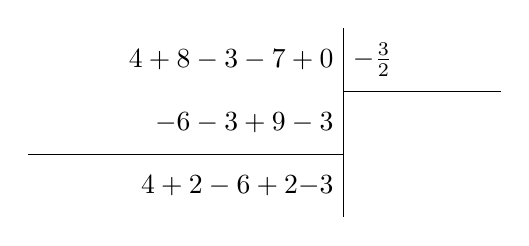
\begin{tikzpicture}[yscale=.8]
\node at (0,0)[left]{$4+8-3-7+0$};
\node at (0,-1)[left]{$-6-3+9-3$};
\node at (0,-2)[left]{$4+2-6+2\boxed{-3}$};
\draw (0,.5)--(0,-2.5);
\draw (0,-.5)--(2,-.5);
\draw (-4,-1.5)--(0,-1.5);
\node at (0,0)[right]{$-\frac{3}{2}$};
\end{tikzpicture}
\end{center}
所以$f(x)$除以$\left(x+\frac{3}{2}\right)$得商式$4x^3+2x^2-6x+2$,余式$-3$.即所求的商式为$q(x)=4x^3+2x^2-6x+2$,余式为$r(x)=-3$.
\end{solution}

容易看出以上两个例子中所得的结果,都符合带余除法恒等式
\[f (x) =q (x) \cdot g (x) +r (x) \]

一般地,多项式带余除法,有以下重要定理:

\begin{blk}{定理}
    对于任意两个多项式$f(x)$, $g(x)\ne 0$, 总是存在唯一的两个多项式$q(x),r(x)$, 使得等式
$f(x) =q(x)\cdot g (x) + r(x) $
成立,并且满足${\rm deg}r(x)<{\rm deg}g(x)$或$r(x)=0$.
\end{blk}

\begin{analyze}
    这个定理的内容既指出了$q(x),r(x)$的存在性——可以找到,又指出了$q(x),r(x)$对于给定的$f(x),g(x)\ne 0$是唯一的——没有第二个.因而,证明理应从这两个方面进行.
\end{analyze}

\begin{proof}
    先证存在性,可按$f(x),g(x)$的次数分为三种情况考虑.
\begin{enumerate}
    \item 若$f(x)=0$, 则不论$g(x)$是什么样的非零多项式,都
可以取$q(x)=r(x)=0$, 显然满足
\[f(x)=q(x)\cdot g(x)+r(x),\quad \text{且}r(x)=0\]
\item 若$f(x)\ne 0$, 且${\rm deg}f(x)<{\rm deg}g(x)$,则可取$q(x)=0$, $r(x)=f(x)$.同样满足
\[f(x)=q(x)\cdot g(x)+r(x),\quad \text{且}{\rm deg}r(x)<{\rm deg}g(x)\]
\item 若$f(x)\ne 0$, 且${\rm deg}f(x)\ge {\rm deg}g(x)$,则可以按下面的方法求出$q(x), r(x)$:

首先用$g(x)$的最高次项去除$f(x)$的最高次项,可得到商$q_1(x)$与余$f_1(x)$,使等式
\begin{equation}
    f (x) =q_1 (x)\cdot y(x)+f_1(x)
\end{equation}
成立,其中$f_1(x)$至少比$f(x)$降低一次,即${\rm deg}f_1(x)<{\rm deg}f(x)$,或$f_1(x)=0$.这时可能有两种情况出现:
\begin{enumerate}
    \item 若${\rm deg}f_1(x)<{\rm deg}g(x)$,或$f_1(x)=0$,我们就取
    \[q(x)=q_1(x),\qquad r(x)=f_1(x)\]
显然定理条件被满足;
\item 若${\rm deg}f_1(x)\ge {\rm deg}g(x)$, 我们就对$f_1(x)$与$g(x)$两个多项式去做上述同样的运算.
\end{enumerate}

其次用$g(x)$的最高次项去除$f_1(x)$的最高次项,可得到商式$q_2(x)$与余式$f_2(x)$, 使等式
\begin{equation}
    f_1(x)=q_2(x)\cdot g(x)+f_2(x)
\end{equation}
成立,其中$f_2(x)$的次数又至少比$f_1(x)$的次数降低一次,即${\rm deg}f_2(x)<{\rm deg}f_1(x)$,或$f_2(x)=0$,这时,
\begin{enumerate}
    \item 若${\rm deg}f_2(x)<{\rm deg}g(x)$,或$f_2(x)=0$,由(3.3)、(3.4)式得
    \[f(x)=[q_1(x)+q_2(x)]\cdot g(x)+f_2(x)\]
    我们就取$q(x)=q_1(x)+q_2(x),\quad r(x)=f_2(x)$.
    定理显然被满足;
    \item 若${\rm deg}f_2(x)\ge {\rm deg}g(x)$,就对$f_2(x)$与$g(x)$做上述同
样运算,同样可以将$f_2(x)$的次数降低至少一次,得到商式$q_3(x)$与余式$f_3(x)$,……作上述同样的分析、处理.
\end{enumerate}

再次,由于${\rm deg}f(x)$是一个非负整数,经过有限次的逐次至少减一,总会有一次(设第$k$次)达到${\rm deg}f_k(x)<{\rm deg}g(x)$或$f_k(x)=0$.于是,我们可得等式
\begin{equation*}
    f_{k-1}(x)=q_k(x)\cdot g(x)+f_k(x) \tag{$k$}
\end{equation*}

综上所述,由等式(3.3)、(3.4)、……($k$),就可以得到
\[\begin{split}
   f(x)&=q_1(x)\cdot g(x)+f_1(x)\\
   &=[g_1(x)+q_2(x)]\cdot g(x)+f_2(x)\\ 
&=\cdots\cdots\\
&=[q_1(x)+q_2(x)+\cdots+q_k(x)]\cdot g(x)+f_k(x)
\end{split}\]
其中,${\rm deg}f_k(x)<{\rm deg}g(x)$或$f_k(x)=0$.

这时,我们就取
\[\begin{split}
    q(x)&=q_1(x)+q_2(x)+\cdots +q_k(x)\\
    r(x)&=f_k(x)
\end{split}\]
显然,这样定理的条件被满足.存在性证毕.
\end{enumerate}

下面再证$q(x)$与$r(x)q$的唯一性.假设除$q(x),r(x)$外,还存在另外一组$q'(x),r'(x)$也满足
\begin{enumerate}
    \item $f(x)=q'(x)\cdot g(x)+r'(x)$,且${\rm deg}r'(x)<{\rm deg}g(x)$或$r'(x)=0$.结合已有的$q(x)$, $r(x)$满足.
    \item $f(x)=q(x)\cdot g(x)+r(x)$,且${\rm deg}r(x)<{\rm deg}g(x)$或$r(x)=0$就可以得出
\[q(x)\cdot g(x)+r(x)=q'(x)\cdot g(x)+r'(x)\]
所以
\[[q(x)-q'(x)]\cdot g(x)=r'(x)-r(x)\]
\end{enumerate}

在此等式中,如果$q(x)-q'(x)\ne 0$,则有
\[{\rm deg}\{[q(x)-q'(x)]\cdot g(x)\}\ge {\rm deg}g(x)\]
但是,由上面的情形又有
${\rm deg}[r'(x)-r(x)]<{\rm deg}g(x)$或$[r'(x)-r(x)]$不定义次数,这是不可能的.所以
\[q'(x)-q(x)=0\quad \Rightarrow\quad q'(x)=q(x)\]

又由于$g(x)\ne 0$,因而$r'(x)-r(x)=0$,即$r'(x)=r(x)$.因此,$q'(x)=q(x)$, $r'(x)=r(x)$.唯一性证毕.
\end{proof}

带余除法是一元多项式的特有运算,但对于二元齐次多项式,我们也可以把其中的一元看作常数来进行带余除法.但是,当余式不为零时,由于选作常数的元的不同,商式与余式也会不同的.

\begin{example}
 已知$f(x,y)=2x^3+7x^2y+13xy^2+5y^3$, $g(x,y)=2x+y$, 试求:
 \begin{enumerate}
     \item 把$y$看作常数时
     \item 把$x$看作常数时
 \end{enumerate}
$f(x,y)$除以$g(x,y)$所得的商式$q(x,y)$与余式$r(x,y)$.
\end{example}

\begin{solution}
\begin{center}
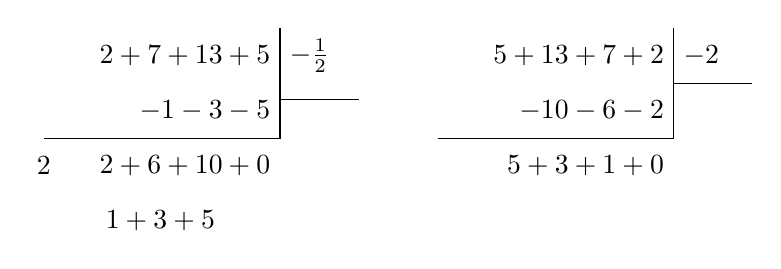
\begin{tikzpicture}[yscale=.7]
\begin{scope}
    \node at (0,0)[left]{$2+7+13+5$};
    \node at (0,-1)[left]{$-1-3-5$};
    \node at (0,-2)[left]{$\boxed{2+6+10}+0$};
    \node at (0,-3)[left]{$1+3+5\qquad $};
    \node at (0,0)[right]{$-\frac{1}{2}$};
    \node at (-3,-2){2};
    \draw (-3,-1.5)--(0,-1.5)--(0,.5);
    \draw (0,-.8)--(1,-.8);
\end{scope}
\begin{scope}[xshift=5cm]
    \node at (0,0)[left]{$5+13+7+2$};
    \node at (0,-1)[left]{$-10-6-2$};
    \node at (0,-2)[left]{$5+3+1+0$};
    \node at (0,0)[right]{$-2$};
    \draw (0,-.5)--(1,-.5);
    \draw (-3,-1.5)--(0,-1.5)--(0,.5);
\end{scope}
\end{tikzpicture}
\end{center}
\begin{enumerate}
    \item $q(x,y)=x^2+3xy+5y^2,\qquad r(x,y)=0$
    \item  $q(x,y)=5y^2+3xy+x^2,\qquad r(x,y)=0$
\end{enumerate}
\end{solution}

\begin{example}
已知$f(x,y)=2x^3+7x^2y+13xy^2+y^3$, $g(x,y)=2x+y$.要求同例3.7.
\end{example}

\begin{solution}
\begin{center}
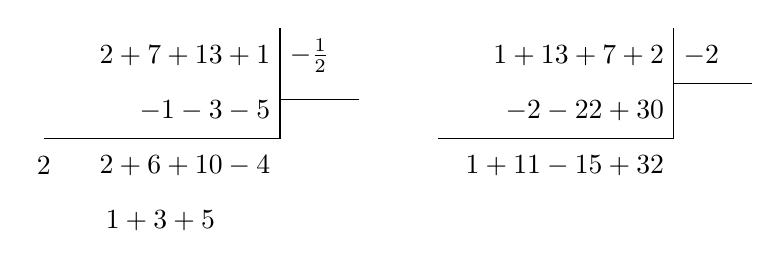
\begin{tikzpicture}[yscale=.7]
\begin{scope}
    \node at (0,0)[left]{$2+7+13+1$};
    \node at (0,-1)[left]{$-1-3-5$};
    \node at (0,-2)[left]{$\boxed{2+6+10}-4$};
    \node at (0,-3)[left]{$1+3+5\qquad $};
    \node at (0,0)[right]{$-\frac{1}{2}$};
    \node at (-3,-2){2};
    \draw (-3,-1.5)--(0,-1.5)--(0,.5);
    \draw (0,-.8)--(1,-.8);
\end{scope}
\begin{scope}[xshift=5cm]
    \node at (0,0)[left]{$1+13+7+2$};
    \node at (0,-1)[left]{$-2-22+30$};
    \node at (0,-2)[left]{$1+11-15+32$};
    \node at (0,0)[right]{$-2$};
    \draw (-3,-1.5)--(0,-1.5)--(0,.5);
    \draw (0,-.5)--(1,-.5);
\end{scope}
\end{tikzpicture}
\end{center}
\begin{enumerate}
    \item $q(x,y)=x^2+3xy+5y^2,\qquad r(x,y)=-4y^3$
    \item  $q(x,y)=y^2+11xy-15x^2,\qquad r(x,y)=32x^3$
\end{enumerate}
\end{solution}

\begin{ex}
\begin{enumerate}
    \item 若$n$次多项式$f(x)$除以$m$次多项式$g(x)$, 试确定所得商式和余式的次数.
    \item 求$f(x)$除以$g(x)$的商式$q(x)$及余式$r(x)$
\begin{enumerate}
    \item $f(x)=x^3+3x^2-x+7,\quad g(x)=x+2$
    \item $f(x)=x^3+3x^2-x+7,\quad g(x)=2x+1$
    \item $f(x)=4x^4+4x^3+5x^2+2x+1,\quad 
g (x) =2x^2+x+1$
    \item $f (x) =x^5+30a^5,\quad g (x) =x+2a$
    \item $f(x)=x^3+3ax^2+(2a^2 -a)x+(a-1),\quad g (x) =x+a-1$
    \item $f(x)=42x^9-13x^7-104x^5+84x^3+9x,\quad 
g (x) =6x^4+11x^2+1$
\end{enumerate}
\item 
若已知除式$g(x)=2x^2-x+3$, 商式$q(x)=x^2-5$, 余式$r(x)=3x+1$, 试求被除式$f(x)$.

\item 试任选一元作常数,求下列$f(x,y)$除以$g(x,y)$所得的商式与余式:
\begin{enumerate}
    \item $f (x,y) =2x^4-x^3y-2x^2y^2-2xy^3-y^4,\quad 
g (x,y) =2x^2+xy+y^2$
    \item $f(x,y)=2x-x^3y-2xy^3-y^4,\quad 
g (x,y) =2x^2+xy+y^2$
\end{enumerate}

\item 求$a^3-b^3+c^3+3abc$除以$a-b+c$所得的商式与余式.
\end{enumerate}
\end{ex}

\section*{习题3.1}
\addcontentsline{toc}{subsection}{习题3.1}
\begin{enumerate}
    \item 试求证
\[\begin{vmatrix}
    a_1+x &  b_1+x  &  c_1+x\\
    a_2+x &  b_2+x  &  c_2+x\\
    a_3+x &  b_3+x  &  c_3+x\\
\end{vmatrix}\]
是一个次数不大于1的多项式或一个零多项式,并求出$p(1)$的值.

\item 不求乘积的各项,只计算下列乘积中$x^{20}$、$x^{12}$两项的系数
\[(a_{13}x^{13}+a_{12}x^{12}+\cdots +a_{1}x+a_0)(b_9x^9+b_8x^8+\cdots +b_1x+b_0)\]
\item 证明恒等式
\[(a^2+b^2)(x^2+y^2)=(ax+by)^2+(bx-ay)^2\]

\item 已知$f(x)=x^7+\frac{1}{128}$, $g(x)=2x+1$,求$f(x)$除以$g(x)$所得的商式$q(x)$及余式$r(x)$.

\item 求$f(x,y)=x^2y+xy^2+xy-x-y-1$除以$g(x,y)=xy-1$所得的商式与余式.
\item 已知
\[\begin{split}
h(x)&=x^2+px+q\\
f(x)&=px^3+(p^2+q)x^2+(2pq+r)x+q^2+s\\
g(x)&=px^3+(p^2-q)x^2+rx-q^2+s
\end{split}\]
试求证:$f(x)$除以$h(x)$, $g(x)$除以$h(x)$分别得到的余式或同时为零,或同时不为零.

\item 如果已知
$f(x)=q(x)\cdot g(x)+r(x)$, 且${\rm deg}r(x)>{\rm deg}g(x)$或$r(x)=0$,$k$是非零常数,试问:
\begin{enumerate}
    \item $kf(x)$除以$g(x)$的商式、余式各是什么?
    \item $f(x)$除以$k\cdot g(x)$商式、余式又是什么?
    \item  $kf(x)$除以$k\cdot g(x)$的商式、余式各是什么?    
\end{enumerate}


\item 已知$f(x)=x^3-2x^2-x+3$, 

试求:$f(-1)$, $f(0)$, $f (x+1) -f (x)$, $f (x^2+1)$.

\item 已知$f(x)=x^4+4x^3+6ax^2+4bx+c$除以$g(x)=x^3+3x^2+9x+3$时的余式$r(x)=0$, 试求$a,b,c$以及商式$q(x)$.

\item 已知$f(x)=x^3+2x^2+3x+2$除以整系数多项式$g(x)$所得的商式和余式都是$h(x)$, 试求$g(x)$与$h(x)$ (其中$h(x)$为非常数的整系数多项式).
\end{enumerate}

\section{余式定理与因式定理}
在初中代数中已经学习过余式定理,它是直接由带余除法引出来的一个重要定理,在代数学中有一系列的理论和应用价值,本节将进一步学习和推广这一定理.

\subsection{余式定理}

对多项式的讨论,可以从形式上作带余除法,从而求得商式及余式;也可以从函数观 点求得在$x$取某一值时的值,这两种观点有什么联系呢?要沟通这两种观点的方法,就是余式定理.

\begin{blk}{余式定理}
    用一次多项式$x-\alpha$去除多项式$f(x)$所得的余式是一个常数,这个常数就等于$f(\alpha)$.
\end{blk}

\begin{proof}
    $f(x)$除以$x-\alpha$,由带余除法得:
\[f(x)=(x-\alpha)\cdot q(x)+r\]
令$x=\alpha$,即得$f(\alpha)=r$,所以
\[f(x)=q(x)\cdot (x-\alpha)+f(\alpha)\]

这样一来,我们若要求$f(x)$除以一次式$x-\alpha$的余式时,除用带余除法外,还可以用余式定理直接求出多项式的值$f(\alpha)$. 两种观点,两种方法的效果是一样的.
\end{proof}

\begin{example}
    试求$f(x)$除以$g(x)=k(x+\alpha)$所得的余式.
\end{example}

\begin{solution}
除式$g(x)=k\left[x-\left(-\frac{\alpha}{k}\right)\right]$

如果设$g_1(x)=x-\left(-\frac{\alpha}{k}\right)$,则$g(x)=k\cdot g_1(x)$,由余式定理可知$f(x)$除以$g_1(x)$所得的余式为
\[r_1=f\left(-\frac{\alpha}{k}\right)\]
    
又根据习题3.1中第7题的结论:除式乘以一个非零数$k$时,余式不变,所以$f(x)$除以$g(x)$所得的余式就等于$f(x)$除以$g_1(x)$所得的余式.所以
\[r=r_1=f\left(-\frac{\alpha}{k}\right)\]
\end{solution}


\begin{example}
    试求$f(x)$除以$g(x)=(x-\alpha)(x-\beta)$的余式.
\end{example}

\begin{solution}
设$f(x)$除以$g(x)$所得的商式为$q(x)$,余式为$r(x)$,则有
\begin{equation}
f(x)=q(x)(x-\alpha)(x-\beta)+r(x)
\end{equation}
    其中,$0\le {\rm deg}r(x)<2$或$r(x)=0$.

因而可进一步设$r(x)=ax+b$,代入(3.5)得
\begin{equation}
    f(x)=q(x)(x-\alpha)(x-\beta)+ax+b
\end{equation}
令$x=\alpha$,由(3.6)得
\begin{equation}
    f(\alpha)=a\alpha+b
\end{equation}
令$x=\beta$,由(3.6)得
\begin{equation}
    f(\alpha)=a\beta+b
\end{equation}
将(3.7), (3.8)联立可以解出
\[a=\frac{f(\alpha)-f(\beta)}{\alpha-\beta},\qquad b=\frac{\alpha f(\beta)-\beta f(\alpha)}{\alpha-\beta}\]
所以,所求的余式为
\[r(x)=\frac{f(\alpha)-f(\beta)}{\alpha-\beta}x+\frac{\alpha f(\beta)-\beta f(\alpha)}{\alpha-\beta}\]
\end{solution}

\begin{ex}
\begin{enumerate}
\item 设$f(x)=x^5-6x^3+x^2-20x+24$, 试求$f(x)$除以下列各式的余数:
\[x-1;\qquad  x+1;\qquad  2x+1;\qquad  3x-2\]
\item 试求
\begin{enumerate}
\item $k\cdot f(x)$除以$x-\alpha$的余式;
\item $(x^2+1)f(x)$除以$x+\beta$的余式;
\item $k(x^2-1)f(x)+3x-1$除以$x-m$的余式.
\end{enumerate}

\item 如果$f(x)$除以$-2$的余式为2, 除以$x+3$的余式为
4, 那么$f(x)$除以$x^2+x-6$的余式是什么?
\end{enumerate}
\end{ex}



\subsection{因式定理}

两个多项式做带余除法时,如果$f(x)$除
以$g(x)$所得的余式$r(x)=0$, 即
\[f (x) =q (x) \cdot g (x) \]
我们就说$f(x)$能被$g(x)$整除,也可以说$g(x)$整除$f(x)$或$g(x)$是$f(x)$的一个因式,$f(x)$是$g(x)$一个倍式.显然,它们的商式$q(x)$也是$f(x)$的一个因式,而$f(x)$也是$q(x)$的一个倍式.

由余式定理可以推证出下列因式定理:

\begin{blk}{因式定理}
$(x-\alpha)$是$f(x)$的一个因式的必要充分条件是$f (\alpha) =0$.
\end{blk}

\begin{proof}
  先证必要性.由于$(x-\alpha)$是$f(x)$的一个因式,因而有
\[f (x) = (x-\alpha ) \cdot q (x) \]
这就是说,$f(x)$除以$x-\alpha$ 时,余式$r=0$.

但由余式定理知,$f(x)$除以$x-\alpha$ 的余式为$f(\alpha )$, 因此,
$f (\alpha) =0$.

再证充分性.由于$f(\alpha )=0$, 因而根据余式定理可以得出
\[f (x) =q (x) \cdot  (x-\alpha ) +f (\alpha ) \]
即
\[f (x) =q (x) (x-\alpha )\]
因此$x-\alpha$ 是$f(x)$的因式.  
\end{proof}


我们已经知道,若在$x=\alpha$ 时,$f(x)$的值$f(\alpha )=0$, 则称$\alpha$ 是$f(x)$的一个根,或者说,$\alpha$是$f(x)$的一个零点.如,
$f(x)=2x^2-7x+3$, 由于$f\left(\frac{1}{2}\right)=f(3)=0$, 因而就说$\frac{1}{2}$,
3都是$f(x)$的根.

这样一来,因式定理又可以叙述为:$(x-\alpha)$是$f(x)$的一个因式的充要条件是$\alpha$ 为$f(x)$的一个
根.

因式定理还可以推广到一般,这就是:

若$(x-\alpha_1)(x-\alpha_2)\cdots(x-\alpha_k)$是$f(x)$的因式的必要充分条件是$f(\alpha_1)=f(\alpha_2) =\cdots=f(\alpha_k)=0$. 也就是$\alpha_1,\alpha_2,\ldots,\alpha_k$都是$f(x)$的根(其中$\alpha_1,\alpha_2,\ldots,\alpha_k$两两不等).

\begin{proof}
必要性是显然的,因为若对于两两不等的数$\alpha_1,\alpha_2,\ldots,\alpha_k$来说,$(x-\alpha_1)(x-\alpha_2)\cdots(x-\alpha_k)$都是$f(x)$的因式,
则有    
\[f(x)=(x-\alpha_1)(x-\alpha_2)\cdots(x-\alpha_k)\cdot q(x)\]
所以$f(\alpha_1)=f(\alpha_2) =\cdots=f(\alpha_k)=0$

即$\alpha_1,\alpha_2,\ldots,\alpha_k$为$f(x)$的$k$个不同的根.

再证充分性,由于$f(\alpha_1)=0$, 因而根据因式定理可
有
\begin{equation}
    f (x) = (x-\alpha_1) \cdot q_1 (x)
\end{equation}

将$x=\alpha_2$代入上式,得
\[f (\alpha_2) = (\alpha_2-\alpha_1) \cdot q_1(\alpha_2)\]
其中,因$f(\alpha_2)=0$, $\alpha_2-\alpha_1\ne 0$, 所以
\[q_1(\alpha_2)=0\]
再根据因式定理,就得出$\alpha_2$是$g_1(x)$的根,即
\begin{equation}
q_1(x)=(a-\alpha_2)\cdot q_2(x)
\end{equation}
将(3.10)代入(3.9)得
\begin{equation}
    f (x) = (x-\alpha_1) (x-\alpha_2)\cdot q_2(x)
\end{equation}
就这样逐步推下去,我们可以得到
\begin{equation}
    f (x) = (x-\alpha_1 ) (x-\alpha_2)\cdots(x-\alpha_{k-1})\cdot q_{k-1}(x) 
\end{equation}
将$x=\alpha_k$代入(3.11)式,得
\[f (\alpha_k) = (\alpha_k -\alpha_1)\cdots (\alpha_k-\alpha_{k-1})\cdot q_{k-1}(\alpha_k)\]
其中,已知$f(\alpha_k)=0$, 且$(\alpha_k-\alpha_1),(\alpha_{k}-\alpha_2),\ldots,(\alpha_k-\alpha_{k-1})$都不等于零,因而有 $q_{k-1}(\alpha_k)=0$.

由因式定理可知$\alpha_k$为$q_{k-1}(x)$的一个根,即
\begin{equation}
    q_{k-1}(x)=(x-\alpha_k)\cdot q_{k}(x)
\end{equation}
将(3.13)式代入(3.12)式,就得出所证结论:
\[f(x)=(x-\alpha_1)(x-\alpha_2)\cdots(x-\alpha_{k-1})(x-\alpha_k)\cdot q_k(x)\]
即:$(x-\alpha_1),(x-\alpha_2),\ldots,(x-\alpha_k)$都是$f(x)$的因式.
\end{proof}

因式定理及推广在沟通两种观点研究多项式的问题上,作用更为突出.数$\alpha$是多项式的一个零点(根)、一次式$(x-\alpha)$是$f(x)$的一个因式、一次式$(x-\alpha)$能够整除$f(x)$、$f(\alpha)=0$都是同一件事情的不同说法,在多项式理论的学习中是很重要的.


\begin{example}
证明恒等式
\[a^2(b-c)+b^2(c-a)+c^2(a-b)=(a-b)(b-c)(c-a)\]
\end{example}

\begin{proof}
等式左边是一个三元多项式,可以分别将$a,b,c$看作元,同时将$b,c$; $a,c$; $b,a$看作常数,依次将$a=b$, $b=c$, $c=a$代入,分别得到
\[\begin{split}
   b^2 (b-c) +b^2 (c-b) +c^2 (b-b) =0\\
   a^2 (c-c) +c^2 (c-a) +c^2 (a-b) =0\\
a^2(b-a)= b^2(a-a) + a^2(a-b) =0 
\end{split}\]

因此,根据因式定理可得
\[a^2 (b-c) +b^2 (c-a) +c^2 (a-b)=k (a-b) (b-c)(c-a)\]
由多项式恒等不难断定$k=1$. 所以
\[a^2 (b-c) +b^2 (c-a) +c^2 (a-b)
= (a-b) (b-c)(c-a)\]
\end{proof}

\begin{example}
    已知$f(x)=x^3+px^2+qx+6$含有因式$(x-3)(x-1)$, 试求$p,q$的值及$f(x)$的另一个一次因式.
\end{example}

\begin{solution}
    由已知可设$f(x)$的另一个一次因式为$ax+b$,因此:
\[f(x)=x^3+px^2+qx+6=(x-3)(x-1)(ax+b)\]
即:
\[x^3+px^2+qx+6=ax^3+(-4a+b)x^2+(3a-4b)x+3b\]
由待定系数法,可以求出
\[a=1,\qquad b=2,\qquad p=-2,\qquad q=-5\]
所以,$f(x)$的另一个一次因式为$x+2$.
\end{solution}

\begin{ex}
\begin{enumerate}
    \item 用因式定理分解因式
\begin{multicols}{2}
\begin{enumerate}
    \item $x^3-3x+2$
    \item $2x^3-x^2-5x-2$
\end{enumerate}
\end{multicols}
    \item 已知$f(x)=3x^3+mx^2+nx-2$含有因式$3x-2$,且$f(-1)=-20$,试求$m,n$的值.
    \item 试证明恒等式
\[a^2(b+c)+b^2(c+a)+c^2(a+b)+2abc=(a+b)(b+c)(c+a)\]
\end{enumerate}  
\end{ex}

\subsection{余式定理、因式定理的推论}

在余式定理与因式定理的基础上,对一元多项式,还有下面两个重要推论:

\begin{blk}{推论1}
    一元$n$次多项式$f(x)$最多只能有$n$个不相同的根.
\end{blk}

\begin{proof}
设$f(x)=a_nx^n+a_{n-1}x^{n-1}+\cdots+a_1x+a_0\quad (a_n\ne 0)$,若已知两两不等的$n$个数
$\alpha_1, \alpha_2, \ldots, \alpha_n$
都是$f(x)$的根,则由因式定理可知
\begin{equation}
    f (x) = (x-\alpha_1) (x-\alpha_2)\cdots (x-\alpha_n)\cdot q(x)
\end{equation}
但由于${\rm deg}f(x)=n$, 且${\rm deg}[(x-\alpha_1)(x-\alpha_2)\cdots(x-\alpha_n)]=n$, 所以(3.14)式中$q(x)$只能是零次多项式,即${\rm deg}g(x)=0$, 再由多项式相等的定义,可知
\[q (x) =a_n\ne 0\]

若再选任一个与$\alpha_i,\; (i=1, 2,\ldots,n)$都不相等的数$\alpha_{n+1}$代入(3.14)式,得
\[f(\alpha_{n+1})=(\alpha_{n+1}-\alpha_{1})(\alpha_{n+1}-\alpha_2)\cdots (\alpha_{n+1}-\alpha_n)\cdot \alpha_n\]
其中,由$\alpha_i,\; (i=1, 2,\ldots,n,n+1)$都不相等,可知
\[\alpha_{n+1}-\alpha_i\ne 0\;  (i=1, 2,\ldots,n),\quad \text{且}\quad a_n\ne 0\]
$\therefore\quad f(\alpha_{n+1}) \ne 0$

因此,$\alpha_{n+1}$不是$f(x)$的根,所以,$f(x)$最多只有$n$个不同根.
\end{proof}

\begin{blk}{推论2}
如果多项式$f(x)$与$g(x)$的次数都不大于$n$, 且有$n+1$个两两不相等的数$\alpha1,\alpha2,\ldots,a_{n+1}$能使这两个多项式相应的值相等,即   
\[f(\alpha_i)=g(\alpha_i)\quad (i=1,2,\ldots,n,n+1)\]
 那么,这两个多项式必定相等,即$f(x)=g(x)$.
\end{blk}

\begin{proof}用反证法.
假设,$f(x)\ne g(x)$, 则多项式
$F (x) =f (x) -g (x)$
就是一个次数不大于$n$的多项式.但是由已知条件知道
\[F (\alpha_i) =f (\alpha_i) -g (\alpha_i)=0,\quad  (i=1,2,\ldots,n,n+1)\]
这就是说,$F(x)$有$n+1$个不同的根.这与推论1的结论是矛盾的.所以
$f (x) =g (x)$.
\end{proof}

\begin{example}
    不用乘法展开下式,求证:
\[x(x-1) (x-2)(x-3)+1=(x^2-3x+1)^2\]
\end{example}

\begin{proof}
    设$f(x)=x(x-1)(x-2)(x-3)+1$, $
g (x) = (x^2-3x+1)^2$.
由于它们都是4次多项式,因而根据推论2,只要验证当$x$取任    
意五个不同的数时,这两个多项式对应的值都相等就可以了,

分别取$x=0, 1, 2, 3, 4$, 则可得:
\[f (0) =1=g (0);\qquad f (1) =1=g (1) ;\qquad f (2) =1=g (2)\]
\[ f (3) =1=g (3) ;\qquad f (4) =25=g (4) \]
所以$f (x) =g (x) $,即:
\[x (x-1) (x-2) (x-3)+1=(x^2-3x+1)^2\]
\end{proof}


\begin{example}
已知$f(x)$是一个五次多项式,且可被$x^2-2$整除,且$f(1)=f(-1)=0$, 试确定这个多项式$f(x)$的各项系数间的关系.
\end{example}

\begin{solution}
设 $f(x)=ax^5+bx^4+cx^3+dx^2+ex+f$,由已知及因式定理可知
\[f (x) = (x^2-2) (x+1)(x-1)\cdot q(x)\]
又由于$f(x)$是五次多项式,因而$q(x)$必定是一次式,不妨设为:$q(x)=mx+n\; (m\ne 0)$.所以
\[ax^5+bx^4+cx^3+dx^2+ex+f= (x^2-2) (x+1)(x-1)(mx+n)\] 
即
\[ax^5+bx^4+cx^3+dx^2+ex+f= mx^5+nx^4-3mx^3-3nx^2+2mx+2n\] 

由多项式相等的定义可得:
\[\begin{cases}
    a=m\\
    b=n\\
    c=-3m\\
    d=-3n\\
    e=2m\\
    f=2n
\end{cases}\qquad (m\ne 0)\]

由此方程组可消去$m,n$,就得
\[\begin{cases}
    a=-\frac{1}{3}x=\frac{1}{2}e\ne 0\\
    b=-\frac{1}{3}d=\frac{1}{2}f
\end{cases}\Rightarrow\quad \begin{cases}
    6a=-2c=3e\ne 0\\
    6b=-2d=3f
\end{cases}\]
这就是$f(x)$的各系数之间的关系.
\end{solution}

\begin{ex}
\begin{enumerate}
    \item 已知$f(1)=f(3)=0$, $f(2)=-4$, 试求二次多项式$f (x)$.
    \item 已知$f(-1)=f(-4)=2$, $f(-3)=8$, $f(-2)=4$.试求三次多项式$f(x)$.
    \item 一个三次多项式$f(x)$, 已知$f(x)+1$可被$(x+1)^2$整除;又$3-f(x)$有一个根为$-2$, 并含有一个因式为一次二项式的平方.试求$f(x)$.
\end{enumerate}
\end{ex}

\section*{习题 3.2}
\addcontentsline{toc}{subsection}{习题 3.2}
\begin{enumerate}
    \item 
已知$f(x)=x^3+3x^2+x+1$, 求$f(x-1)$, $f(x+1)$, $f (-x^2)$
\item 已知$f(x-1)=x^3+3x^2+x-1$, 求$f(x)$, $f(-x)$.
\item 已知$f(x)=x^3+ax^2+5x-4$, 且$f(2)=f(-3)$, 试求$a$及$f(2)$.
\item 若有一多项式$g(x)$, 已知$g(-1)=1$, $g(4)=11$, 试求$f(x)$被$(x+1)(x-4)$除后的余数.

\item 如果$f(x)$被$2x-3$除以后余数为4, 试求多项式
$(x^2+1)\cdot f(x)+7$被$2x-3$除的余数.
\item 已知恒等式
\[x^3+x^2+x+1=a+b (x+1) +c (x+1) (x+3)+d (x+1) (x+3)(x+5)\]
试求$a,b,c,d$的值.
\item 用余式定理及其推论证明:
\[\begin{split}
   & (b-c) (x-b)(x-c)+(c-a)(x-c)(x-a)\\
&\qquad + (a-b) (x-a)(z-b)+(a-b)(b - c)(c-a)=0
\end{split}\]
\item 证明$2b^2c^2+2c^2a^2+2a^2b^2-a^4-b^4-c^4$ 能被$(a+b+c)(b+c-a)(c+a-b)(a+b-c)$整除,
并求其商式.
\item 若$f(x)=x^3+kx^2-20x+6$ 能被$x-3$整除,试求常
数$k$.
\item 若$f(x)=2x^3-x^2+ax+b$能被$(x+2)(x-4)$整除,
试求常数$a,b$.
\item $f(x)=2x^3-ax+1$, $g(x)=x^3+5x+b$ 能不能有四个不同的数$\alpha_1,\alpha_2,\alpha_3,\alpha4$, 使得$f (\alpha_i) =g (\alpha_i)\quad  (i=1,2,3,4)$,
为什么?
\item 利用因式定理,分解因式
\begin{enumerate}
    \item $x^3-3x+2$
    \item $x^3-(a+2b)x^2+b(2a+b)x-ab^2$
\end{enumerate}

\item 如果$x^2+5xy+ay^2+x-y-2=f(x,y)$可以分解为$x,y$的一次因式的积,试求$a$的值.
\end{enumerate}

\section{最高公因式与辗转相除法}
关于两个多项式的公因式、最高公因式的概念,我们在初中代数中已经学过,同时,我们还学习过用辗转相除、分解因式两种方法去求最高公因式,还学习了两个多项式的公倍式与最低公倍式以及求最低公倍式的方法,并得出了最低,公倍式与最高公因式之间的关系
\[[f(x),g(x)]=\frac{k\cdot f(x)\cdot g(x)}{(f(x)\cdot g(x))}\]

由于最高公因式与辗转相除法在多项式理论中占有重要地位,本节将重点进一步加深学习这两个内容.

\subsection{最高公因式}

首先,我们在已经学习的基础上,较严格地给出最高公因式的定义:

\begin{blk}{定义}
 对给定的非零多项式$f(x),g(x)$, 如果有一个多项式$d(x)$, 能满足以下三个条件:   
\begin{enumerate}
    \item $d(x)$的首项系数为1,
    \item $d(x)$是$f(x)$与$g(x)$的公因式,
    \item $d(x)$是$f(x)$与$g(x)$的其它任何一个公因式$\ell(x)$
    的倍式,即$f(x)$与$g(x)$的任一公因式$\ell(x)$是$d(x)$的因式.那么,$d(x)$就叫做多项式$f(x)$与$g(x)$的最高公因式,一般记作
    $(f (x) ,g (x) ) =d (x)$
\end{enumerate}
\end{blk}

上述的条件1是为了保证$(f(x),g(x))$的唯一性而提出的.事实上,若$d(x)$, $d_1(x)$都是$f(x)$与$g(x)$的最高公因式,则由条件2、3就可得出$d(x)$与$d_1(x)$能互相整除,这就有$d(x)=kd_1(x)$, 再由条件1就得到$d(x)=d_1(x)$. 这
就说明,$(f(x),g(x))$如果存在,一定是唯一的.

我们还知道,若$f(x),g(x)$都已分解成不可约的因式的乘积,则在$f(x),g(x)$的所有公因式中,取每一个公因式的指数较小者,这些因式的乘幂的乘积,再乘以一个能使其首项系数为1的常数,就是$(f(x),g(x))$.这就是我们常用的求最高公因式的视察法.


\begin{example}
$f(x)=x(2x-1)^4(x+3)^3$,$g(x)=x^2(2x-1)^2(x+2)^2$

试求$(f(x),g(x))$
\end{example}

\begin{solution}
    公因式为$x,2x-1$,$x$的指数$f(x)$中的1,$2x-1$的指数取$g(x)$中的2,得:
\[(f(x),g(x))=k\cdot x (2x-1)^2\]
$k$是待定系数,为使$(f(x),g(x))$的首期系数为1,显然应取$k=\frac{1}{4}$,所以
\[(f(x),g(x))=\frac{1}{4}  x (2x-1)^2\]
\end{solution}

\begin{example}
$f(x)=x^2-3x+2$, $g(x)=x^4-3x^3+5x^2-8x+5$

试求$(f(x),g(x))$
\end{example}

\begin{solution}
由视察知,$f(x)=(x-1)(x-2)$,因而$(f(x),g(x))$不可能有$(x-1)$, $(x-2)$外的因式,再由因式定理,求得$g(1)=0,\; g(2)\ne 0$,所以$x-1$是$f(x), g(x)$唯一的公因式.所以
\[(f(x),g(x))=x-1\]
\end{solution}

\begin{blk}{定理1}
    给定非零多项式$f(x),g(x)$, 对于任意两个多项式$u(x),v(x)$来说,$f(x),g(x)$的公因式也一定是
$u(x)\cdot f(x)+v(x)\cdot g(x)$的因式.
\end{blk}

\begin{proof}
  设$d(x)$是$f(x)$与$g(x)$的一个公因式,则
\[f (x) =d (x) \cdot f_1 (x),\qquad  g(x)=d(x)\cdot g_1(x)\]
所以
\[u (x) \cdot f (x) +v (x) \cdot g (x) =d (x) [u (x) \cdot f_1 (x) +v (x) \cdot g_1 (x) ]\]
即$d(x)$也是$u(x)\cdot f(x)+v(x)\cdot g(x)$的一个因式.  
\end{proof}

\begin{example}
已知$f(x)=x^4-x^3+3x^2-4x-12$, $g(x)=x^4-x^3+2x^2+3x-22$.

求$(f(x),g(x))$.
\end{example}

\begin{analyze}
应用定理1的结论,我们可以取$u(x)=1$, $v(x)=-1$,从而可得 $f(x)-g(x)=x^2-7x+10$. 只要从 $x^2-7x+10$的因式中就可以找出$f(x),g(x)$的公因式的范围,再应用因式定理即可确定$(f(x),g(x))$.
\end{analyze}

\begin{solution}
因为$f(x)-g(x)=x^2-7x+10=(x-2)(x-5)$,所以$f(x),g(x)$的一次公因式只可能是$x-2$与$x-5$,于是由因式定理,求得
$f(2)=g(2)=0$,但$f(5)\ne 0$.所以$(f(x),g(x))=x-2$.
\end{solution}

\begin{example}
    已知$f(x)=2x^3-3x^2-3x+2$, $g(x)=3x^3-2x^2-7x-2$.求$(f(x),g(x))$.
\end{example}

\begin{solution}
    因为$f(x)+g(x)=5x^3-5x^2-10x=5x(x+1)(x-2)$其中$x$显然不是$f(x),g(x)$的公因式,再用综合除法求得
\[x+1|f(x),\qquad x+1|g(x),\qquad x-2|f(x),\qquad x-2|g(x)\]
所以
\[(f(x),g(x))=(x+1)(x-2)\]
\end{solution}

\begin{ex}
    求下列各组多项式的最高公因式:
\begin{enumerate}
    \item $f(x)=\poly{1,0,0,-1},\quad g(x)=\poly{1,2,3,2,1}$
    \item $f(x)=2x^3-3x^2-11x+6,\quad g(x)=\poly{4,3,-9,2}$
    \item $f(x)=\poly{2,-5,0,-2,1},\quad g(x)=\poly{2,-7,6,-4,1}$
\end{enumerate}
\end{ex}

\subsection{辗转相除法}

辗转相除法的理论基础在于多项式的带余除法及本节的定理1.

\begin{blk}{定理2}
    对于非零多项式$f(x)$, $g(x)$, $r(x)$, 若存在多项式$q(x)$使得$f(x)=q(x)\cdot g(x)+r(x)$, 则有
    \[\big(f(x),\; g(x)\big)=\big(g(x),\; r(x)\big)\]
\end{blk}

\begin{proof}
设$\big(g(x),\; r(x)\big)=d(x)$,则
\begin{enumerate}
\item $d(x)$首项系数是1;
\item $d(x)$是$g(x)$, $r(x)$的公因式,由定理1可知,
$d(x)$也是$f(x)$的因式,因而也是$f(x),g(x)$的公因式;    
\item 再设$f(x)$, $g(x)$的任一个公因式为$\ell(x)$, 由于$r(x)=f(x)-q(x)\cdot g(x)$, 所以,$\ell(x)$也是$r(x)$的一个因式,因而$\ell(x)$就是$g(x),r(x)$的公因式,再由最高公因式的定义知,$\ell(x)$是$d(x)$的因式.所以
\[\big(f (x) ,g (x) \big) =d (x) = \big(g (x) ,r (x) \big)\]
\end{enumerate}
\end{proof}

这样一个定理对于求两个已知多项式的最高公因式起到一些什么作用呢?两个多项式中总有一个多项式的次数不大于另一个多项式的次数,不妨设$g(x)$设的次数不大于$f(x)$的次数,则因在带余除法中,$r(x)$的次数小于$g(x)$的次数或$r(x)=0$. (注意,定理2并不要求$r(x)$满足带余除法中对余式的要求,但带余除法中的余式满足定理2中$r(x)$的条件)这就说明$r(x)$的次数小于$f(x)$的次数,把求$\big(f(x), g(x)\big)$转化为求$\big(g(x), r(x)\big)$实际上是一个降次的过程.

次数是降低了,那么有没有把握求出$\big(g(x),r(x)\big)$呢?
现在可以对$g(x)$, $r(x)$再进行带余除法,求出又一个余
式$r_2(x)$(为了易于辨别,我们把第一次余式记为$r_1(x)$,类似地把第一次第二次所得的商式分别记为$q_1(x)$, $q_2(x)$, 以后以此类推),循此以往,可得到一系列的带余除法:
\begin{equation}
    \begin{split}
f(x)&=q_1(x)g(x)+r_1(x),\quad {\rm deg}r_1(x)<{\rm deg}g(x)\\
g(x)&=q_2(x)r_1(x)+r_2(x),\quad {\rm deg}r_2(x)<{\rm deg}r_1(x)\\
r_1(x)&=q_3(x)r_2(x)+r_3(x),\quad {\rm deg}r_3(x)<{\rm deg}r_2(x)\\
r_2(x)&=q_4(x)r_3(x)+r_4(x),\quad {\rm deg}r_4(x)<{\rm deg}r_3(x)\\
\cdots &\cdots \cdots \cdots \\
r_{i-1}(x)&=q_{i+1}(x)r_i(x)+r_{i+1}(x),\quad {\rm deg}r_{i+1}(x)<{\rm deg}r_i(x)\\
\cdots &\cdots \cdots \cdots \\
r_{s-1}(x)&=q_{s+1}(x)r_s(x)
\end{split}
\end{equation}

最后一个等式表示$r_s(x)$整除$r_{s-1}(x)$, 或者说$r_{s+1}(x)=0$.此时就有
\[\begin{split}
    \big(f(x), g(x)\big)&=\big(g(x),r_1(x)\big)=\big(r_1(x),r_2(x)\big)=\cdots\\
    &=\big(r_i(x),r_{i+1}(x)\big)=\cdots\\
    &=\big(r_{s-1}(x),r_s(x)\big)
\end{split}\]

显然有$\big(r_{s-1}(x),r_s(x)\big)=\frac{1}{c}r_s(x)$,其中:$c$是$r_s(x)$首项系
数.因此:
\[\big(f(x), g(x)\big)=\frac{1}{c}r_s(x)\]

自然会提出这样一个问题,如果始终不能整除,怎么办?我们来证明不会出现始终不能整除的情况.

设${\rm deg}g(x)$是一个有限的非负整数$m$.若$r_1(x)\ne 0$, 令${\rm deg}r_i(x)=m_i$,则
\[m>m_1>m_2>\cdots>m_i>\cdots>m_{s-1}>m_s\]
注意到$m$和所有$m_i$都是非负整数,而数列$m,m_1,m_2,\ldots,m_i,\ldots$
是一个严格递减的数列,则这个数列一定是有限的.例如$m=100$时,数列最多不会超过101项.在某种情形下,若$m_s=0$, 即$r_s(x)$是一个非零常数时,$r_s(x)$就整除$r_{s-1}(x)$了.在这种情况下,$\big(f(x),g(x)\big)=1$, 我们说$f(x)$与$g(x)$互质.这就说明,即使$f(x)$, $g(x)$互质,它们的最高公因式1仍可由上述累次的带余除法求得,由此我们得到:

\begin{blk}{定理3(辗转相除法定理)}
  任给两个非零多项式$f(x)$, $g(x)$进行(3.15)式所给出的辗转相除,通过有限次的运算总可求出唯一存在的$\big(f(x),g(x)\big)$.
\end{blk}

 存在性已在前面叙述,至于唯一性则在给出$\big(f(x),g(x)\big)$的定义后即已阐明.  

\begin{example}
$f(x)=\poly{6,-4,-11,-3,-3,-1}$, 

$g(x)=\poly{4,2,-18,3,-5}$

求$\big(f(x),g(x)\big)$
\end{example}

\begin{solution}
\begin{center}
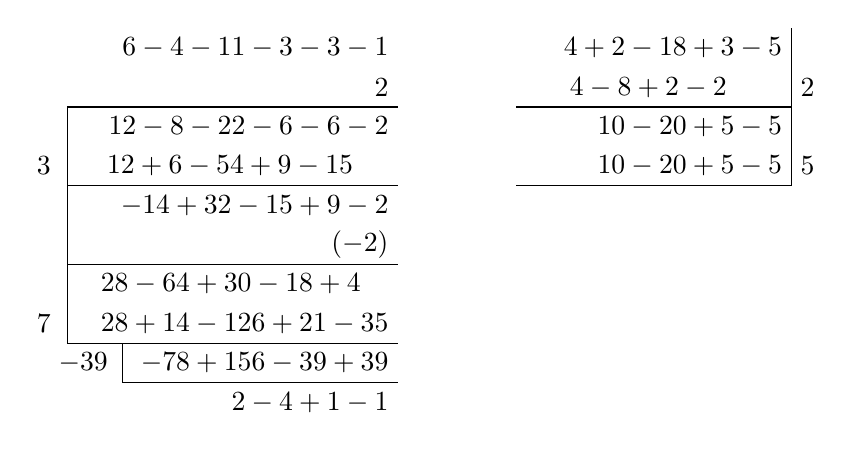
\begin{tikzpicture}
\begin{scope}
\node at (0,0)[left]{$6-4-11-3-3-1$};
\node at (0,-0.5)[left]{$\x 2$};
\node at (0,-1)[left]{$12-8-22-6-6-2$};
\node at (0,-1.5)[left]{$12+6-54+9-15\quad\;$};
\node at (0,-2)[left]{$-14+32-15+9-2$};
\node at (0,-2.5)[left]{$\x(-2)$};
\node at (0,-3)[left]{$28-64+30-18+4\quad$};
\node at (0,-3.5)[left]{$28+14-126+21-35$};
\node at (0,-4)[left]{$-78+156-39+39$};
\node at (0,-4.5)[left]{$2-4+1-1$};

\foreach \x in {-.75, -1.75, -2.75, -3.75}
{
    \draw (-4.2,\x)--(0,\x);
}
\draw (-3.5,-4.25+.5)--(-3.5,-4.25)--(0,-4.25);
\draw (-4.2,-.75)--(-4.2,-3.75);
\node at (-4.5,-1.5){3};
\node at (-4.5,-3.5){7};
\node at (-4,-4){$-39$};
\end{scope}
\begin{scope}[xshift=5cm]
    \node at (0,0)[left]{$4+2-18+3-5$};
\node at (0,-0.5)[left]{$4-8+2-2\qquad $};
\node at (0,-1)[left]{$10-20+5-5$};
\node at (0,-1.5)[left]{$10-20+5-5$};
\foreach \x in {-.75, -1.75}
{
    \draw (-3.5,\x)--(0,\x);
}
\draw (0,-1.75)--(0,.25);
\node at (.2,-.5){2};
\node at (.2,-1.5){5};
\end{scope}
\end{tikzpicture}
\end{center}    

所以$\big(f(x),g(x)\big)=\frac{1}{2}(\poly{2,-4,1,-1})$.
\end{solution}

在习题3.1第7题中,我们知道对被除式$f(x)$乘以非零常数$k$, 给予$r(x)$的影响也不过是乘一个常数$k$, 而我们所求的最后的$r_s(x)$本来就得乘以$\frac{1}{c}$($c$是$r_s(x)$的首项系数)才成为
$\big(f(x),g(x)\big)$, 所以实际上对$\big(f(x),g(x)\big)$完全没有影响,即使对部分余式$f_1(x)$(如例3.19)的$-14x^4+3x^3-15x^2+9x-2$乘以非零常数$k$, 对$\big(f(x),g(x)\big)$也没有影响,因为$\big(f(x),g(x)\big)=\big(f_1(x),g(x)\big)$在辗转相除法中,实际上我们已把求$\big(f(x),g(x)\big)$转化为求$\big(f_1(x),g(x)\big)$, (注意在定理2中,并未要求${\rm deg}r(x)<{\rm deg}g(x)$,
所以$f_1(x)$又起一个被除式的角色,因而乘以非零常数$k$,对于所得的$r(x)$仍不过相关一个常数因子,而这一点上面已说明对$\big(f(x),g(x)\big)$不会有影响的.

辗转相除法是一个运算过程较繁的方法.如果$f(x)$, $g(x)$很容易分解因式,或者说如果$f(x)$与$g(x)$这两个多项式中至少有一个很容易分解成不可约因式的乘积,我们当然宁愿用分解因式的方法来求这两个多项式的最高公因式.但是多项式的因式分解并不总能做到.例如把一个三次多项式与一个四次多项式相乘,求出作为乘积的七次多项式是轻而易举的;但反过来,给出一个七次多项式,要求分解成两个次数较低的多项式的乘积,一般是很难做到的.相比之下,辗转相除法尽管较繁,却是有效、能算,总能求出两个多项式的最高公因式.再进一步考察任何一个多项式的不可约因式分解的表达式,是否总存在.如果存在,是否唯一,我们在以前的学习中并未作出结论.将来的进一步学习可以对这个问题作出肯定的答案.而这个结论要通过一系列命题的推导才能得出,辗转相除法之有效、能算恰恰是推导这一系列命题的基础之一.因此,从理论上来,辗转相除法是不可替代的重
要的数学方法.

我们还可以看到,用辗转相除法求两个多项式的最高公因式的过程实际上是不断地进行带余除法的过程,而带余除法的运算只包括多项式的加法、减法,乘法及非零数之间的除法以及单项式相除的指数运算律.这些在以有理数为系数的多项式集合中或是在以实数为系数的多项式集合中都是封闭的.因此,我们不难得出这样的结论:两个有理系数多项式的最高公因式仍是一个有理系数多项式,两个实系数多项式的最高公因式仍是一个实系数多项式.

\begin{example}
$f(x)=\poly{1,0,-10,0,1}$,\quad  $g(x)=\poly{1,-4\sqrt{2},6,4\sqrt{2},1}$

求$\big(f(x),g(x)\big)$
\end{example}

\begin{solution}
\begin{center}
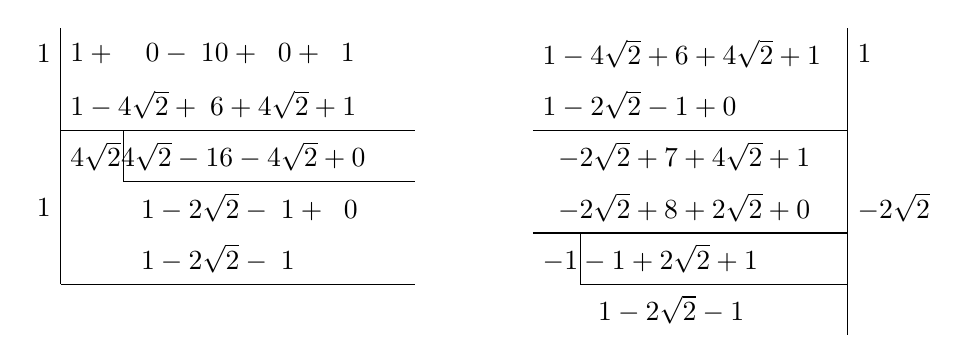
\begin{tikzpicture}[yscale=1.3]
\begin{scope}
\node at (0,0)[right]{$1+\quad 0-\; 10+\;\; 0+\;\; 1$};
\node at (0,-0.5)[right]{$1-4\sqrt{2}+\;6+4\sqrt{2}+1$};
\node at (0,-1)[right]{$4\sqrt{2} 4\sqrt{2}-16-4\sqrt{2}+0$};
\node at (0,-1.5)[right]{$\qquad\;\; 1-2\sqrt{2}-\;1+\;\;0$};
\node at (0,-2)[right]{$\qquad\;\; 1-2\sqrt{2}-\;1$};
\draw (0,.25)--(0,-2.25);
\draw (0,-.75)--(4.5,-.75);
\draw (.8,-.75)--(.8,-1.25)--(4.5,-1.25);
\draw (0,-2.25)--(4.5,-2.25);
\node at (0,0)[left]{1};
\node at (0,-1.5)[left]{1};
\end{scope}

\begin{scope}[xshift=6cm]
    \node at (0,0)[right]{$1-4\sqrt{2}+6+4\sqrt{2}+1$};
\node at (0,-0.5)[right]{$1-2\sqrt{2}-1+0$};
\node at (0,-1)[right]{$\;\;-2\sqrt{2}+7+4\sqrt{2}+1$};
\node at (0,-1.5)[right]{$\;\;-2\sqrt{2}+8+2\sqrt{2}+0$};
\node at (0,-2)[right]{$-1-1+2\sqrt{2}+1$};
    \node at (0,-2.5)[right]{$\qquad 1-2\sqrt{2}-1$};
\draw (4,.25)--(4,-2.75);
\draw(0,-.75)--(4,-.75);
\draw(0,-1.75)--(4,-1.75);
\draw(.6,-1.75)--(.6,-2.25)--(4,-2.25);
\node at (4,0)[right]{1};
\node at (4,-1.5)[right]{$-2\sqrt{2}$};
\end{scope}
\end{tikzpicture}
\end{center}
所以$\bigl(f(x),g(x)\bigr)=x^2-2\sqrt{2}x-1$.
\end{solution}


\begin{ex}
求$\bigl(f(x),g(x)\bigr)$:
\begin{enumerate}
    \item $f(x)=\poly{1,-7,13,3,-18}$
    
$g(x)=\poly{1,-5,2,20,-24}$
\item $f(x)=\poly{1,-7,-22,139,105}$
    
$g(x)=\poly{1,-8,-11,116,70}$
\item $f(x)=\poly{1,1,1,2},\quad g(x)=\poly{1,0,-1,-1}$
\end{enumerate}
\end{ex}

\section*{习题3.3}
\addcontentsline{toc}{subsection}{习题3.3}

\begin{enumerate}
    \item $f(x)=\poly{2,3,6,4,3},\quad g(x)=\poly{2,-5,-6,-12,-9}$

求:$\bigl(f(x),g(x)\bigr)$及$\bigl[f(x),g(x)\bigr]$.其中$\bigl[f(x),g(x)\bigr]$为$f(x)$与$g(x)$的最低公倍式.

\item $f(x)=\poly{2,3,-4,13,-6},\quad g(x)=\poly{2,-1,2,3,-2}$

$h(x)=\poly{1,3,1,5,6}$

求:$\bigl(f(x),g(x),h(x)\bigr)$

\item $f(x)=\poly{1,a,b,1},\qquad g(x)=\poly{1,b,a,1}$

求证:$(f,g)=1$,除非$a=b$或$a+b+2=0$.
\item $f(x)=\poly{2,-3,1},\qquad g(x)=\poly{3,-2,1}$

利用辗转相除法中关系式(3.15)的逆推,找出两个多项式$\mu(x)$, $\nu(x)$使下式成立:
\[\mu(x)\cdot f(x)+\nu(x)\cdot g(x)=(f,g)\]

\item $f(x)=\poly{2,-1,2},\qquad g(x)=\poly{1,1,1}$

试求两个多项式$\mu(x)$, $\nu(x)$使下式成立:
\[\mu(x)\cdot f(x)+\nu(x)\cdot g(x)=1\]

\item $m,n$是大于1的自然数,求$f(x)=x^m-1$及$g(x)=x^n-1$
的最高公因式.
\end{enumerate}


\section{插值公式}
如果$n$次多项式$f(x)$在取$n+1$个不同值时的函数值已给出,应用余式定理推论2就可以求出唯一的多项式函数$f(x)$. 在$f(x)$是一次多项式时,$y=ax+b$的图象是一条直线,推论2对于这个一次函数的论断的几何意义就是“两点确定一直线”.在一般情形下,一个$n$次多项式函数$y=f(x)$的曲线,由其所过的$n+1$个点所唯一确定,反之,仅给$n+1$个横坐标不同的点,总可以唯一确定一个次数不大于$n$的多项式函数$y=f(x)$的曲线.在数学中,这样的唯一性定理常常是计算问题解决问题的基本依据.这一节就讨论这样一些问题.

\subsection{余式定理推论的应用举例}
\begin{example}
    已知$f(2)=8$, $f(3)=f(4)=f(5)=0$, 求次数不大于3的多项式$f(x)$.
\end{example}

\begin{analyze}
如果设$f(x)=ax^3+bx^2+cx+d$, 用$x=2, 3,
4, 5$四个数相继代入,然后解四元一次方程组求出$a,b,c,d$. 虽然肯定可以求出来,但计算量太大.现已知中有有利条件:$f(3)=f(4)=f(5)=0$, 我们就可以应用因式定理把问题简化.
\end{analyze}

\begin{solution}
    由已知$f(3)=f(4)=f(5)=0$,因而可以
    设$f(x)=(x-3)(x-4)(x-5)q(x)$.
    
    由于$(x-3)(x-4)(x-5)$已是3次,而$f(x)$的次数
不大于3, 所以$q(x)$应为常数,即
\[f(x)=a_3(x-3)(x-4)(x-5)\]
再以$x=2$代入,得$3=-6a_3$,因此:$a_3=-\frac{1}{2}$

\[\therefore\quad f(x)=-\frac{1}{2}(x-3)(x-4)(x-5)\]
\end{solution}


\begin{example}
已知:$f_1(2)=3$, $f_1(3)=f_1(4)=f_1(5)=0$, $f_2(3)=6$, $f_2(2)=f_2(4)=f_2(5)=0$, $f_3(4)=-3$, $f_3(2)=f_3(3)=f_3(5)=0$, $f_4(5)=12$, $f_4(2)=f_4(3)=f_4(4)=0$

求四个次数不大于3的多项式$f_1(x)$, $f_2(x)$, $f_3(x)$, $f_4(x)$.
\end{example}

\begin{solution}
    解法同例3.21,可得
\[\begin{split}
    f_1(x)&=-\frac{1}{2}(x-3)(x-4)(x-5)\\
    f_2(x)&=3(x-2)(x-4)(x-5)\\
    f_3(x)&=\frac{3}{2}(x-2)(x-3)(x-5)\\
    f_4(x)&={2}(x-2)(x-3)(x-4)\\
\end{split}\]
\end{solution}

以上两例说明在已知函数值有若干个为零时,充分应用因式定理可以减少对待定系数的繁杂的计算量.(若一开始就令$f(x) =a_3a^3+a_2x^2+a_1x+a_0$, 就得解关于待定系数 $a_3,a_2,a_1,a_0$的四元一次方程组).在已知函数值中没有零,或者很少为零的情况下,我们可以把所求的多项式$f(x)$分解为若干个多项式的和其中每一个多项式的函数值只有一个非零数.


\begin{example}
    已知$f(2)=3$, $f(3)=6$, $f(4)=-3$, $f(5)=12$, 求次数不大于3的多项式$f(x)$.
\end{example}

\begin{analyze}
    实际上$f(x)$正是例中四个多项式的和.
\end{analyze}

\begin{solution}
  令$f_1(x),f_2(x),f_3(x),f_4(x)$分别如例3.22中的已知条件所述,$F(x)=f_1(x)+f_2(x)+f_3(x)+f_4(x)$, 则
\[    F (2) =f_1 (2) +f_2 (2) +f_3 (2) +f_4 (2) =3+0+0+0=3\]

    同样可求得$F(3)=6$, $F(4)=-3$, $F(5)=12$, 可见:
\[\begin{split}
    f(x)=F(x)&=-\frac{1}{2} (x-3) (x-4)(x-5)+3 (x-2) (x-4)(x-5)\\
    &\qquad 
    +\frac{3}{2} (x-2) (x-3)(x-5)
   +2 (x-2) (x-3)(x-4)   
\end{split}\]    
\end{solution}



\begin{example}
    已知$\alpha_i\; (i=1, 2, 3, 4)$是四个两两不等的数.$c_i\; (i=1, 2, 3, 4)$是另外四个数.试求次数不大于3的多项式$f(x)$, 使得$f (\alpha_i) =c_i,\; (i=1, 2, 3, 4)$ 
\end{example}

\begin{solution}
    与例3.23的处理方法相类似,可假设四个多项式
$f_1(x),f_2(x),f_3(x),f_4(x)$,$f_i(\alpha_j)=\delta_{ij}c_i$    
    
    此处$$\delta_{ij}=\begin{cases}
        1,& i=j\\
        0,& i\ne j
    \end{cases}\quad  (i,j=1, 2, 3, 4)$$
则显然有$f(x)=f_1(x)+f_2(x)+f_3(x)+f_4(x)$.
还可以简记为$$f(x)=\sum^4_{i=1}f_i(x)$$
其中,$f_i(x)=k(x-\alpha_2)(x-\alpha_3)(x-\alpha_4)$

$\because\quad f_1(\alpha_1)=c_1$

$\therefore\quad k_1=\frac{c_1}{(\alpha_1-\alpha_2)(\alpha_1-\alpha_3)(\alpha_1-\alpha_4)}$

\[\therefore\quad f_1(x)=\frac{c_1(x-\alpha_2)(x-\alpha_3)(x-\alpha_4)}{(\alpha_1-\alpha_2)(\alpha_1-\alpha_3)(\alpha_1-\alpha_4)}\]
同理可求得:
\[\begin{split}
    f_2(x)&=\frac{c_2(x-\alpha_1)(x-\alpha_3)(x-\alpha_4)}{(\alpha_2-\alpha_1)(\alpha_2-\alpha_3)(\alpha_2-\alpha_4)}\\
    f_3(x)&=\frac{c_3(x-\alpha_1)(x-\alpha_2)(x-\alpha_4)}{(\alpha_3-\alpha_1)(\alpha_3-\alpha_2)(\alpha_3-\alpha_4)}\\
    f_4(x)&=\frac{c_4(x-\alpha_1)(x-\alpha_2)(x-\alpha_3)}{(\alpha_4-\alpha_1)(\alpha_4-\alpha_2)(\alpha_4-\alpha_3)}
\end{split}\]
因此:
\[\begin{split}
f(x)&=\frac{c_1(x-\alpha_2)(x-\alpha_3)(x-\alpha_4)}{(\alpha_1-\alpha_2)(\alpha_1-\alpha_3)(\alpha_1-\alpha_4)}+\frac{c_2(x-\alpha_1)(x-\alpha_3)(x-\alpha_4)}{(\alpha_2-\alpha_1)(\alpha_2-\alpha_3)(\alpha_2-\alpha_4)}\\
&\quad +\frac{c_3(x-\alpha_1)(x-\alpha_2)(x-\alpha_4)}{(\alpha_3-\alpha_1)(\alpha_3-\alpha_2)(\alpha_3-\alpha_4)}+\frac{c_4(x-\alpha_1)(x-\alpha_2)(x-\alpha_3)}{(\alpha_4-\alpha_1)(\alpha_4-\alpha_2)(\alpha_4-\alpha_3)}
\end{split}\]
还可以简单记为:
\[f(x)=\sum^4_{i=1} c_i\frac{(x-\alpha_1)(x-\alpha_2)\cdots (x-\alpha_{i-1})(x-\alpha_{i+1})\cdots (x-\alpha_4)}{(\alpha_i-\alpha_1)(\alpha_i-\alpha_2)\cdots (\alpha_i-\alpha_{i-1})(\alpha_i-\alpha_{i+1})\cdots (\alpha_i-\alpha_4)}\]
\end{solution}


\begin{example}
$\alpha_1,\alpha_2,\alpha_3$表三个两两不等的数,试用$f(\alpha_1)$, $f(\alpha_2)$, $f(\alpha_3)$来表示$(x-\alpha_1)(x-\alpha_2)(x-\alpha_3)$除多项式$f(x)$所得的余式.
\end{example}

\begin{solution}
\[f(x)=(x-\alpha_1)(x-\alpha_2)(x-\alpha_3)q(x)+r(x)\]
并且:${\rm deg}r(x)\le 2$或$r(x)=0$,则
\[r(\alpha_1)=f(\alpha_1),\qquad r(\alpha_2)=f(\alpha_2),\qquad r(\alpha_3)=f(\alpha_3)\]
 仿照上例可得:
 \[\begin{split}
     r(x)&=f(\alpha_1)\frac{(x-\alpha_2)(x-\alpha_3)}{(\alpha_1-\alpha_2)(\alpha_1-\alpha_3)} +f(\alpha_2)\frac{(x-\alpha_1)(x-\alpha_3)}{(\alpha_2-\alpha_1)(\alpha_2-\alpha_3)}
     \\
&\quad     +f(\alpha_3)\frac{(x-\alpha_1)(x-\alpha_2)}{(\alpha_3-\alpha_1)(\alpha_3-\alpha_2)}
 \end{split}\]
\end{solution}

\begin{ex}
\begin{enumerate}
    \item 已知$f(1)=f(2)=f(3)=2$, $f(0)=-16$.求三次多项式$f(x)$.
    \item 已知$f(-3)=42$, $f(-2)=6$, $f(-1)=0$, $f(0)=0$, $f(1)=6$.求四次多项式$f(x)$.
\end{enumerate} 
\end{ex}

\subsection{插值公式}

把上述例题所得的结果予以推广,应有
下列定理:

\begin{blk}{定理}
    设$f(x)$是一个次数不大于$n$的多项式,$\alpha_i\; (i=1, 2,\ldots,n,n+1)$表示$n+1$个两两不等的数,$b_i\; (i=1, 2,\ldots,n,n+1)$是任意$n+1$个数,而且
$f (\alpha_i) =b_i,\; (i=1, 2,\ldots,n,n+1)$,则:
\[\begin{cases}
   f(x)=\sum^{n+1}_{i=1} f_i(x)\\
   f_i(x)=b_i\frac{(x-\alpha_1)\cdots(x-\alpha_{i-1})(x-\alpha_{i+1})\cdots (x-\alpha_{n+1})}{(\alpha_i-\alpha_1)\cdots(\alpha_i-\alpha_{i-1})(\alpha_i-\alpha_{i+1})\cdots (\alpha_i-\alpha_{n+1})}
\end{cases}\]
\end{blk}

\begin{proof}
令$f_i(x)$是由下列条件所唯一确定的次数不大于$n$的多项式:
\[f_i(\alpha_j)=\delta_{ij}b_i,\qquad \delta_{ij}=\begin{cases}
    1&i=j\\
    0&i\ne j
\end{cases}\quad (i,j=1,2,\ldots,n+1)\]
则由因式定理可知
\[f_i(x)=c_i(x-\alpha_1)\cdots(x-\alpha_{i-1})(x-\alpha_{i+1})\cdots (x-\alpha_{n+1})\]
由$f_i(\alpha_i)=b_i$定出$c_i$的值,可得
\[c_i=\frac{b_1}{(\alpha_i-\alpha_1)\cdots(\alpha_i-\alpha_{i-1})(\alpha_i-\alpha_{i+1})\cdots (\alpha_i-\alpha_{n+1})}\]
$\therefore\quad f_i(x)=b_i\frac{(x-\alpha_1)\cdots(x-\alpha_{i-1})(x-\alpha_{i+1})\cdots (x-\alpha_{n+1})}{(\alpha_i-\alpha_1)\cdots(\alpha_i-\alpha_{i-1})(\alpha_i-\alpha_{i+1})\cdots (\alpha_i-\alpha_{n+1})}$

显然有 $f(x)=\displaystyle\sum^{n+1}_{i=1} f_i(x)$.
\end{proof}

上述公式叫做拉格朗日的插值公式.

\begin{example}
   令$g_n(x)$为一个$n$次多项式,它在$0, 1,\ldots,n-1,n $时的值分别为$0, 0,\ldots,0, 1$, 求$g_n(x)$. 
\end{example}

\begin{solution}
    由插值公式直接得出
    \[\begin{split}
        g_n(x)&=\frac{x(x-1)(x-2)\cdots(x-n+1)}{1\cdot 2\cdots n}\\
        &=\frac{x(x-1)\cdots(x-n+1)}{n!}      
    \end{split}\]

$n!$对非负整数$n$都有定义,读作“$n$阶乘”,当$n>0$时,
$n!=1\x2\x\cdots \x n$, 并规定$0!=1$.

注意$g_n(x)$是应用插值公式最容易求出的多项式,我们以后将会有意识地引进这样的多项式.
\end{solution}

\begin{example}
    已知$f(x)$是一个次数不大于3的多项式,$f(0)=1$, $f(1)=4$, $f(2)=15$, $f(3)=40$, 不求出$f(x)$, 直接计算$f(1.5)$.
\end{example}

\begin{solution}
    由插值公式可知
    \[\begin{split}
         f (1. 5) &=1\cdot \frac{(1. 5-1) (1.5-2)(1.5-3)}{(0-1) (0-2)(0-3)}+4\cdot \frac{(1.5-0)(1.5-2)(1.5-3)}{(1-0) (1-2)(1-3)}\\
         &\quad +15\cdot \frac{(1. 5-0) (1.5-1)(1.5-3)}{(2-0) (2-1)(2-3)} +40\cdot \frac{(1. 5-0) (1.5-1)(1.5-2)}{(3-0) (3-1)(3-2)}\\
         &=8.125
    \end{split}\]
\end{solution}
 

\begin{example}
某人身旁没有三角函数表(或带有三角函数的计算器),却需要计算$\sin23^{\circ}$, 他记得一些特殊角的三角函数:
\[\sin0^{\circ}=0,\qquad \sin15^{\circ}=\frac{1}{4} (\sqrt{6}-\sqrt{2}) =0. 259,\qquad \sin30^{\circ}=0.5\]
\[\sin45^{\circ}=\frac{\sqrt{2}}{2}=0. 707,\qquad \sin60^{\circ}=\frac{\sqrt{3}}{2}=0.866\]
他根据这些数据把函数$y=f(x)=\sin x$近似地看成一个次数不大于4的多项式,问如此计算出来的$\sin23^{\circ}$是多少?
\end{example}

\begin{solution}
    由已知$f(0)=0$, $f(15)=0. 259$, $f(30)=0. 5$, $f(45)=0. 707$, $f(60)=0. 866$, 求$f(23)$.

方法同例3.26
\[\begin{split}
    f(23)&=0. 259\x \frac{23 (23-30) (23-45)(23-60)}{15 (15-30) (15-45)(15-60)}\\
    &\quad +0. 5\x \frac{23 (23-15) (23-45)(23-60)}{30 (30-15) (30-45)(30-60)}\\
&\quad +0. 707\x \frac{23 (23-15) (23-30)(23-60)}{45 (45-15) (45-30)(45-60)}\\
&\quad +0.866\x \frac{23 (23-15) (23-30)(23-45)}{60 (60-15) (60-30)(60-45)}\\
&\approx \frac{23}{15^4}\x (246+814-244+44) \approx 0. 391
\end{split}\]

实际上从三角函数表上査出的 $\sin23^{\circ}$如果要求精确到0.001也是0.391.
\end{solution}

关于一个函数为什么可以近似地用多项式来代替,在什么条件下才可以近似地用多项式来代替,我们到学习微积分时再加以研究.这里只说明插值公式有这样一个“插值”的应用.

\begin{ex}
    \begin{enumerate}
    \item 已知$f(0)=0$, $f(1)=1$, $f(2)=2$, $f(3)=3$,
    $f(4)=4$, 试求一个次数不大于4的多项式$f(x)$.
    \item 已知$f(0)=0$, $f(1)=1$, $f(2)=2$, $f(3)=3$,
    $f(4)=4$, 若求一个多项式$f(x)$, 没有说明其次数不大于4, 能否得出$f(x)=x$的结论?为什么?举一个反例.
    \item 已知$f(x)$是一个二次多项式,$f(1)=3$, $f(2)=6$, $f(8)=13$, 计算$f(1. 5)$.
    \item 为了计算$\sqrt{26}$, 只记得$\sqrt{2}=1. 414$, $\sqrt{3}=1. 732$, 因而算得$\sqrt{24}=4.898$, $\sqrt{25}=5$, $\sqrt{27}=5. 196$, 试由这三个数据近似地计算出$\sqrt{26}$(精确到0.001).
    \end{enumerate} 
    \end{ex}
    
    \section*{习题3.4}
    \addcontentsline{toc}{subsection}{习题3.4}
    \begin{enumerate}
        \item 已知$f(4)=0$, $f(6)=-12$, $f(7)=-20$,
        $f(8)=-18$, 求次数尽可能小的多项式$f(x)$, 然后计算$f(12)$.
        \item 当$x=2, 3, 4, 5$时,$f(x)$的值分别为$5, 4,-7,-34$, 求三次多项式$f(x)$.
        \item 已知$5x^2+19x+18=\frac{a}{2}(x-2)(x-3)-b(x-3)(x-1)+\frac{c}{2}(x-1)(x-2)$, 计算$a,b,c$这三个数
        对多项式$5x^2+19x+18$ 来说有些什么意义?
        \item $a,b,c$是两两不等的三个数,已知$f(a)=bc$, $f(b)=
        ca$, $f(c)=ab$, 求次数不超过2的多项式$f(x)$.
        \item $a,b,c$是两两不等的三个数,已知$f(a)=b+c$, $f(b)=
        c+a$, $f(c)=a+b$, 求次数不超过2的多项式$f(x)$.
    \end{enumerate}
    
    \section{多项式的导数与换元展开式}
    在本节里,我们将引进多项式的导数概念及其简单性质.并学习多项式的换元展开式,进一步把余式定理推广,为今后研究多项式函数在某定点邻近的区域内的局部性质打下一定基础.
    
    \subsection{多项式的导数}
    导数概念是微积分学中的重要概
    念,这里仅就多项式来讨论,我们规定:
    
\begin{blk}{定义1}
对任意的非负整数$n$, 单项式$ax^n$
的导数就是单项式$nax^{n-1}$.
\end{blk}    

     
\begin{blk}{定义2}
对任意的非零多项式
$f (x) =a_nx^n+a_{n-1}x^{n-1}+\cdots+a_1x+a_0$
的导数就是各项导数的代数和,记作
\[f' (x) =na_nx^{n-1}+(n-1)a_{n-1}x^{n-2}+\cdots +a_1\]

同样,$f'(x)$的导数,记作
\[f'' (x) =n (n-1) a_nx^{n-2} + (n-1) (n-2)a_{n-1}x^{n-3}+\cdots+a_2\]
叫做多项式$f(x)$的二阶导数;
$f''(x)$的导数,记作$f'''(x)$,叫做$f(x)$的三阶导数,也是$f'(x)$的二阶导数;一般地,$f'(x)$的$k-1$阶导数,就是
$f(x)$的$k$阶导数,记作$f^{(k)}(x)$,即:
\[\left[f^{(k-1)} (x)\right]'=f^{(k)}(x)\]
\end{blk}    

   \begin{example}
    求 $f(x)=2x^3-8x^2+5x-4$的各阶导数.
    \end{example}

    \begin{solution}
\[\begin{split}
    f' (x) &=6x^2-16x+5\\
        f'' (x) &=12x-16\\
        f''' (x) &=12\\
        f'''' (x) &=f^{(5)}(x)=\cdots =f^{(n)}(x)=0,\qquad (n\ge 4)
\end{split}\]
    \end{solution}    

    显然,一元$n$次多项式的$n$阶导数是一个非零常数(零次多项式),从$n+1$阶系数开始,以后各高阶导数都是零;
    特别地,零次多项式的导数等于零;而零多项式的各阶导数仍是零.

    总之,多项式的导数仍然是多项式.而且对于系数在整数,有理数,实数范围内的各多项式集合,求导数这种运算也是封闭的.

 
    \begin{example}
求多项式$f (x) =a_3x^3+a_2x^2+a_1x+a_0\quad  (a_3\ne 0)$ 的各阶导数,并求出各阶导数在$x=x_0$时的值.          
    \end{example}           
         
    \begin{solution}
\[\begin{split}
 f'(x)&=3a_3x^2+2a_2x+a_1\qquad 
    f' (x_0) =3a_3 x^2_0 +2a_2x_0+a_1\\
    f'' (x) &=6a_3x+2a_2\qquad \qquad \quad 
    f'' (x_0) =6a_3x_0+2a_2\\
    f''' (x) &=6a_3\qquad \qquad \qquad \qquad 
     f''' (x_0 ) =6a_3\\
     f^{(4)} (x)&=f^{(5)}(x)=\cdots =f^{(n)}(x)=0\\
     f^{(4)}  (x_0)&=f^{(5)}(x_0)=\cdots =f^{(n)}(x_0)=0 
\end{split}\] 
    \end{solution} 

容易证明,多项式的导数有以下性质:

\begin{blk}{性质1}
    多项式$f(x)$与常数$k$乘积的导数等于$f(x)$的导数与$k$的乘积,即
\[[kf (x) ]'=k\cdot f' (x) \]
\end{blk}   

\begin{proof}
设$f(x)=a_nx^n+a_{n-1}x^{n-1}+\cdots+a_1x+a_0$,
则
\[kf(x)=ka_nx^n+ka_{n-1}x^{n-1}+\cdots+ka_1x+ka_0\]
因此:
\[\begin{split}
    [kf(x)]'&=kna_nx^{n-1}+k(n - 1)a_{n-1}x^{n-2}+\cdots+ka_1\\
&=k \left[na_nx^{n-1}+(n - 1)a_{n-1}x^{n-2}+\cdots+a_1\right]\\
&=kf' (x) 
\end{split}\]
\end{proof}

\begin{blk}{性质2}
    两多项式$f(x),g(x)$和的导数等于这两个多项式的导数和,即
\[[f (x) +g (x) ]'=f' (x) +g' (x) \]  
\end{blk}  
 
\begin{proof}
设$f(x)=a_nx^n+a_{n-1}x^{n-1}+\cdots+a_1x+a_0$,$g(x)=b_mx^m+b_{m-1}x^{m-1}+\cdots+b_1x+b_0$,不失一般性,不妨设$n>m$,则有
\[f(x)+g(x)=a_nx^n+\cdots + (a_{m}+b_m)x^{m}+\cdots+(a_1+b_1)x+a_0+b_0\]
因此:
\[\begin{split}
    [f(x)+g(x)]'&=na_nx^{n-1}+\cdots + m(a_{m}+b_m)x^{m-1}+\cdots+a_1+b_1\\
    &=(na_nx^{n-1}+\cdots+ma_mx^{m-1}+\cdots +a_1)+(mb_mx^{m-1}+\cdots +b_1)\\
    &=f'(x)+g'(x)
\end{split}\]
\end{proof}  

综合性质1, 2, 就可以得出:对任意的两个常数$\mu$, $\lambda$和多项式$f(x),g(x)$, 下述等式是成立的,即
\[[\mu\cdot f (x) +\lambda\cdot g (x) ]'=\mu f' (x) +\lambda g' (x) \]

\begin{blk}{性质3}
两个多项式$f(x),g(x)$的乘积的导数等于$f(x)$的导数乘以$g(x)$与$g(x)$的导数乘以$f(x)$的和,即
\[[f (x) g (x) ]'=f' (x) g (x) +g' (x) f (x) \]
\end{blk}

\begin{blk}{性质4}
    一个多项式$f(x)$的$m$次方的导数为
\[[f^m (x) ] '= mf^{m-1} (x) f' (x) \]
\end{blk}

性质3, 4的证明亦可以像前两个性质一样通过实际计算进行,但较繁,这里略去不证,同学们可通过练习验证.

\begin{example}
求下列多项式的导数:
\begin{enumerate}
    \item $f(x)=g(x)h(x)$
    \item $f (x) =g^2 (x) +2g (x) h (x) +h^2 (x) $
\end{enumerate} 
这里$g(x)=3x^2-1$, $h (x) =8x^3+2x-1$
    \end{example}

    \begin{solution}
\begin{enumerate}
    \item $f(x)=(3x^2-1)(8x^3+2x-1)$
\[\begin{split}
    f' (x) &= (3x^2-1)' (8x^3+2x-1)+(8x^3+2x-1)' (3x^2-1) \\
    &=6x (8x^3+2x-1) + (24x^2+2) (3x^2-1)\\
    &=48x^4+12x^2-6x+72x^4-18x^2-2\\
    &=120x^4-6x^2-6x-2
\end{split}\]
    \item $f(x)=g^2 (x) +2g (x) h (x) +h^2 (x) =[g(x)+h(x)]^2=(8x^3+3x^2+2x-2)^2$
\[\begin{split}
    f'(x)&=2(8x^3+3x^2+2x-2)(8x^3+3x^2+2x-2)'\\
    &=2(8x^3+3x^2+2x-2)(24x^2+6x+2)\\
    &=\poly{384,240,164,-60,-16,-8}
\end{split}\]
\end{enumerate}
 \end{solution}
           
\begin{ex}
\begin{enumerate}
    \item 求下列各多项式的各阶导数
\begin{multicols}{2}
\begin{enumerate}
    \item $f (x) =3x^2+x-2$
    \item $f(x) =ax^2+bx+c$
    \item $f(x)=\frac{4\cdot 3}{2!}a^2x^2$
\end{enumerate}
\end{multicols}

    \item 对于$f(x)=a_3x^3+a_2x^2+ax+a_0,\quad g(x)=b_2x^2+b_1x+b_0$
    
    验证导数的性质3是成立的.

    \item 求下列各多项式的导数:
\begin{multicols}{2}
\begin{enumerate}
    \item $f (x) =\varphi^2 (x) +1$
    \item $f(x)=\varphi(x)g(x)$
    \item $f (x) =\varphi^3 (x) g (x)$
    \item $f(x)=\varphi^2(x)-g^2(x)$
\end{enumerate}
\end{multicols}
这里$\varphi(x)=x-2,\quad g(x)=3x^3+5x-1$.
    \item 试试看:你能证明“如果$(x-a)^k$能够整除$f(x)$, 那么$(x-a)^{k-1}$一定能够整除$f'(x)$吗”?
\end{enumerate}
\end{ex}
 
\subsection{多项式的换元展开式——泰勒公式}

 在初中代数
中,我们曾经学习过用综合除法的方法,将任一个非零次多项式$f(x)$展开成$(x-a)$的幂的形式.如果令$x-a=t$则$x=a+t$将它代入$f(x)$后,即可将$f(x)$展开成元$t=(x-a)$的幂的形式,按升幂排列成:
\[f (x) =f (a+t) =c_0+c_1t+c_2t^2+\cdots+c_nt^n\]
就叫做多项式$f(x)$在$x=a$点的换元展开式.

这里的待定系数$c_i,\; (i=0, 1, 2,\ldots,n)$ 显然只与$f(x)$
和所选定的点$a$有关.以下我们就复习用综合除法确定这些系数的方法,并进一步研究这些系数的一般规律,得出一般公式.

    \begin{example}
        用综合除法,将$f (x) =2x^2-x-2$展开成$x-1$的幂的形式.
    \end{example}    
    
    \begin{solution}
  用$x-1$去连续除$f(x)$, 由综合除法得
\begin{center}
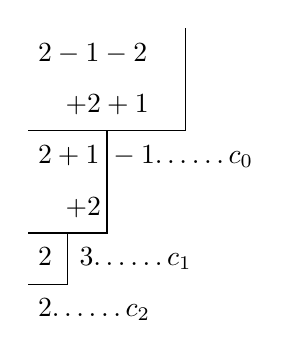
\begin{tikzpicture}[yscale=1.3]
    \node at (0,0)[right]{$2-1-2$};
    \node at (0,-0.5)[right]{$\quad +2+1$};
    \node at (0,-1)[right]{$2+1\; -1 $……$c_0$};
    \node at (0,-1.5)[right]{$\quad +2$};
    \node at (0,-2)[right]{$2\quad 3$……$c_1$};
    \node at (0,-2.5)[right]{$2$……$c_2$};
\draw (0,-.75)--(2,-.75)--(2,.25);
\draw (0,-1.75)--(1,-1.75)--(1,-.75);
\draw (0,-2.25)--(.5,-2.25)--(.5,-1.75);
\end{tikzpicture}
\end{center}

\[\therefore\quad f (x) =-1+3 (x-1) +2 (x-1)^2\]
或
\[f (1+t) =-1+3t+2t^2,\qquad (x-1=t)\]
\end{solution}
   
\begin{example}
已知$f(x)=a_3x^3+a_2x^2+a_1x+a_0$, 试求:
\begin{multicols}{2}
\begin{enumerate}
    \item $f (1+t)$
    \item $f(x_0+t)$
\end{enumerate}
\end{multicols}
\end{example}

\begin{solution}
\begin{enumerate}
    \item 
这就是要求当$x=1+t$, 即$t=x-1$时$f(x)$的换元展开,可以用综合除法
\begin{center}
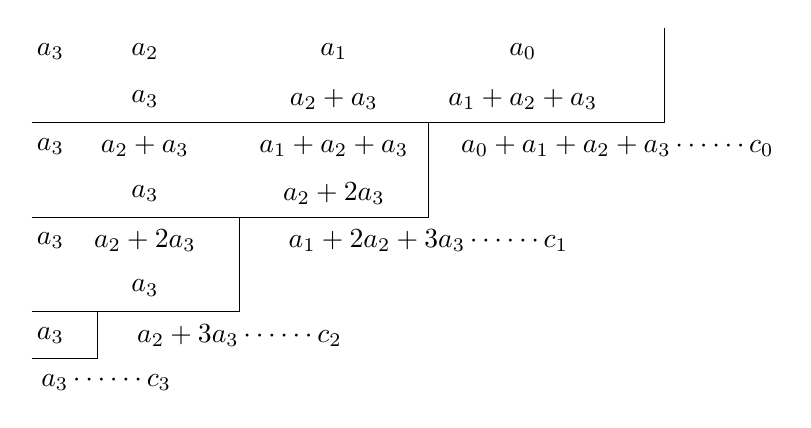
\begin{tikzpicture}[scale=1.2]
\foreach \x/\xtext in {0/a_3,1/a_2,3/a_1,5/a_0}
{
    \node at (\x,0){$\xtext$};
}
\foreach \x/\xtext in {0/{},1/a_3,3/a_2+a_3,5/a_1+a_2+a_3}
{
    \node at (\x,-0.5){$\xtext$};
}
\foreach \x/\xtext in {0/a_3,1/a_2+a_3,3/a_1+a_2+a_3,6/a_0+a_1+a_2+a_3\cdots\cdots c_0}
{
    \node at (\x,-1){$\xtext$};
}
\draw(-.2,-.75)--(6.5,-.75)--(6.5,.25);
\foreach \x/\xtext in {1/a_3,3/a_2+2a_3}
{
    \node at (\x,-1.5){$\xtext$};
}
\draw(-.2,-1.75)--(4,-1.75)--(4,-.75);
\foreach \x/\xtext in {0/a_3,1/a_2+2a_3,4/a_1+2a_2+3a_3\cdots\cdots c_1}
{
    \node at (\x,-2){$\xtext$};
}
\node at (1,-2.5){$a_3$};
\draw(-.2,-2.75)--(2,-2.75)--(2,-1.75);
\foreach \x/\xtext in {0/a_3,2/a_2+3a_3\cdots\cdots c_2}
{
    \node at (\x,-3){$\xtext$};
}
\node at (-.2,-3.5)[right]{$a_3\cdots\cdots c_3$};
\draw(-.2,-3.25)--(.5,-3.25)--(.5,-2.75);

\end{tikzpicture}
\end{center}
因此:
\[\begin{split}
    f (x) &= (a_0+a_1 +a_2 +a_3) + (a_1 +2a_2+3a_3 ) (x-1)\\
    &\qquad +(a_2 +3a_3) (x-1)^2+a_3(x-1)^3\\
f(1+t)&=(a_0+a_1 +a_2 +a_3) +(a_1 +2a_2+3a_3)t \\
&\qquad + (a_2+3a_3) t^2+a_3t^3
\end{split}\]

\item 直接换元,令$x=x_0+t$代入$f(x)$, 并展开整理成$t$
的升幂排列形式
\[\begin{split}
    f (x_0+t) &=a_3(x_0+t) +a_2(x_0+t)^2+a_1(x_0+t)+a_0\\
&=(a_0 +a_1x_0 +a_2x_0^2+a_3x_0^3) + (a_1+2a_2x_0+3a_3 x^2_0)t\\
&\qquad + (a_2+3a_3x_0) t^2+a_3t^3
\end{split} \]
\end{enumerate}
\end{solution}

为了找出换元展开式中待定系数$c_i\; (i=0, 1,\ldots,n)$的一般规律,我们对例3.33(2)分析并验证如下:

换元展开式中的常数项$a_0+a_1x_0+a_2x_0^2+a_3x_0^3$正好是$x=x_0$时,多项式$f(x)$的值$f(x_0)$. 例3.32及例3.33(1)也是 如此;$c_0=f (x_0)$.

换元展开式中的一次项系数 $a_1+2a_2x_0+3a_3x_0^2$正好是$x=x_0$时多项式$f(x)$的导数$f'(x)=3a_3x^2+2a_2x+a_1$的值$f'(x_0)=a_1+2a_2x_0+3a_3x_0^2$.例3.32及例3.33(1)也是如此;
$c_1 =f' (x_0)$.

换元展开式中的二次项系数 $a_2+3a_3x_0$正是$x=x_0$时,
$f(x)$的二阶导数$f'(x)=6a_3x+2a_2$的值的一半:$\frac{1}{2}f''(x_0)=a_2+3a_3x_0$.例3.32及例3.33(1)也是如此;$c_2=\frac{1}{2}f''(x_0)$.

换元展开式中的三次项系数$c_3$, 也容易分析出它正是当$x=x_0$时,$f(x)$的三阶导数$f'''(x)=6a_1$的值的六分之一,$\frac{1}{6}f'''(x_0)=a_3$, 可验证例3.33(1)也是如此;
$c_3=\frac{1}{6}f''' (x_0)$.

这样一来,利用导数概念,换元展开式就可以写成:
\[f(x_0+t)=f(x_0)+f'(x_0)t+\frac{1}{2}f''(x_0)t^2+\frac{1}{6}f'''(x_0)t^3\]    
进而可写成更有规律、便于记忆的形式
\[f(x_0+t)=f(x_0)+\frac{f'(x_0)}{1!}t+\frac{f''(x_0)}{2!}t^2+\frac{f'''(x_0)}{3!}t^3\]    
同样,例3.33(1)的换元展开写成
\[f (1+t) =f (1) +\frac{f'(1)}{1!}t+\frac{f''(1)}{2!}t^2+\frac{f'''(1)}{3!}t^3\]
例3.32 也可以写成
\[f (1+t) =f (1) +\frac{f'(1)}{1!}t+\frac{f''(1)}{2!}t^2=-1+3t-2t^2\]

实际上,这正是多项式换元展开式的一般规律,推广到$n$次多项式就得到重要的泰勒定理.
    
\begin{blk}{定理(泰勒定理)}
 一元$n$次多项式$f(x)$在点$x_0$
的换元展开式为
\begin{equation}
    f(x_0+t)=f(x_0)+\frac{f'(x_0)}{1!}t+\frac{f''(x_0)}{2!}t^2+\cdots+\frac{f'''(x_0)}{n!}t^n
\end{equation}   
\end{blk}

定理的一般证明这里略去,但容易验证,这个定理的内容对于零多项式、零次多项式都是适合的;对二、三次多项式我们从例3.32和例3.33也已验证过是适合的,对于其它高次多项式以后再给出确切证明,现在可以应用.

    \begin{example}
已知$f(x)=\poly{1,0,-2,3,5}$,试求$f(x)$在$x=1$点的展开式.    
    \end{example}    
    
    \begin{solution}
\begin{center}
\begin{tabular}{lll}
$f(x)=\poly{1,0,-2,3,5}$  &  $f(1)=7$  \\
$f'(x)=\poly{4,0,4,3}$  &  $f'(1)=3$  \\
$f''(x)=\poly{12,0,-4}$  &  $f''(1)=8$& $\frac{8}{2}=4$  \\
$f'''(x)=24x$  &  $f'''(1)=24$ & $\frac{24}{3!}=4$\\
$f''''(x)=24$  &  $f''''(1)=24$ & $\frac{24}{4!}=1$\\
\end{tabular}    
\end{center}

$\therefore\quad f(1+t)=7+3t+4t^2+4t^3+t^4$.又由于$x=a+(x-a)$,因此:
\begin{equation}
    \begin{split}
    f(x)&=f[a+(x-a)]\\
    &=f(a)+\frac{f'(a)}{1!}(x-a)+\frac{f''(a)}{2!}(x-a)^2+\cdots+\frac{f^{(n)}(a)}{n!}(x-a)^n
\end{split}
\end{equation}
(3.17)式叫做多项式$f(x)$在点$x=a$的换元展开式.
    \end{solution}

(3.16)与(3.17)本质上是相同的,都叫做泰勒公式,只是(3.16)式中的$t$相当于(3.17)式中的$x-a$罢了,不过在今后应用更多的是(3.17)式.

 \begin{example}
    已知$f(x)=x^5+2x^4-2x^3+7x-5$, 试将$f(x)$展开成$x+1$的升幂多项式.
    \end{example}

    \begin{solution}    
\begin{center}
\begin{tabular}{lll}
$f(x)=\poly{1,2,-1,0,7,-5}$  &  $f(-1)=-10$  \\
$f'(x)=\poly{5,8,-3,0,7}$  &  $f'(-1)=1$  \\
$f''(x)=\poly{20,24,-6,0}$  &  $f''(-1)=10$& $\frac{10}{2!}=5$  \\
$f'''(x)=\poly{60,48,-6}$  &  $f'''(-1)=6$ & $\frac{6}{3!}=1$\\
$f^{(4)}(x)=120x+48$  &  $f^{(4)}(-1)=-72$ & $\frac{-72}{4!}=-3$\\
$f^{(5)}(x)=120$  &  $f^{(5)}(-1)=120$ & $\frac{120}{5!}=1$\\
\end{tabular}    
\end{center}
          
$\therefore\quad f(x)=-10+(x-1)+5(x-1)^2+(x-1)^3-3(x-1)^4+(x-1)^5$
    \end{solution}

    还可以用连续作综合除法的方法,得出同样的结果.同学们可以验证一下.

\begin{ex}
\begin{enumerate}
    \item 试用秦勒公式将下列多项式在给定点展开成升幂形式:
\begin{enumerate}
    \item $g(x)=\poly{7,-3,4,-1}$,在$x=2$点;
    \item $f (x) =9x^5-188$,在$x=-2$点;
    \item $h(x)=x^4-x^2-1$,在$x=-1$点.
\end{enumerate}

    \item 试用泰勒公式将下列多项式展开成指定一次式的升幂形式:
\begin{enumerate}
    \item $f(x)=2x-2x^2+x^3$, 展成$x-1$的幂;
    \item $g(x)=2x^3+24x^2+34x+30$, 展成$x+2$的幂;
    \item $h(x)=28x-27+x^3-9x^2$展成$x-3$的幂.
\end{enumerate} 
\end{enumerate}
\end{ex}
    
\subsection{余式定理的推广}

泰勒公式,实际上就是通过多
项式的恒等变形,把一个以$x$为元的多项式变换为一个以
$x-a$为元的升幂多项式.

有了泰勒公式,我们可以更深刻,更一般地去理解余式定理.

由泰勒公式
\[f(x)=f(a)+\frac{f'(a)}{1!}(x-a)+\frac{f''(a)}{2!}(x-a)^2+\cdots+\frac{f^{(n)}(a)}{n!}(x-a)^n\]
可以直观看出:
\begin{enumerate}
    \item 若用$x-a$去除$f(x)$, 所得余式为$r_1(x)=f(a)$, 这正是我们在第二节所学的余式定理的内容;
    \item 若用$(x-a)^2$去除$f(x)$, 所得的余式为
    \[ r_2(x) =f (a) +\frac{f'(a)}{1!}  (x-a)\]
    这就要比余式定理的内容进一步了;
    \item 一般地,若用$(x-a)^k\; (k\le n)$除$f(x)$, 所得的余式为
    \[r_k(x)=f(a)+\frac{f'(a)}{1!}(x-a)+\cdots+\frac{f^{(k-1)}(a)}{(k-1)!}(x-a)^{k-1}\]
    这就是余式定理推广的结论.
\end{enumerate}

    \begin{example}
试求$f(x)=\poly{1,0,-2,8,5}$除以$g(x)=(x-1)^3$所得的余式$r(x)$.
    \end{example}    
    
    \begin{solution}
\begin{center}
\begin{tabular}{lll}
$f(x)=\poly{1,0,-2,8,5}$  &  $f(1)=12$  \\
$f'(x)=\poly{4,0,-4,8}$  &  $f'(1)=8$  \\
$f''(x)=\poly{12,0,-4}$  &  $f''(1)=8$& $\frac{8}{2!}=4$  \\
\end{tabular}    
\end{center}
          
$\therefore\quad f(x)$除以$g(x)$所得的余式为
\[\begin{split}
    r(x)&=f(1)+\frac{f'(1)}{1!}(x-1)+\frac{f''(1)}{2!}(x-1)^2\\
    &=12+8(x-1)+4(x-1)^2\\
    &=12-8+8x+4x^2-8x+4\\
    &=4x^2+8
\end{split}\]
    \end{solution}

    \begin{example}
已知一个首项系数是2的三次多项式 $g(x)$除以$(x-2)^3$所得的余式为$2x^2+x-1$, 试求这个多项式$g(x)$.
    \end{example}    
    
    \begin{solution}
设$g(x)=f(2)+\frac{f'(2)}{1!}(x-2)+\frac{f''(2)}{2!}(x-2)^2+\frac{f'''(2)}{3!}(x-2)^3$

由已知,$g(x)$的首项(最高次项)系数为2, 可得
\[\frac{f'''(2)}{3!}=2\quad \Rightarrow\quad f'''(2)=12\]

又由$g(x)$除以$(x-2)^3$所得余式为$2x^2+x-1$, 可以
得       
\[f(2)+\frac{f'(2)}{1!}(x-2)+\frac{f''(2)}{2!}(x-2)^2=2x^2+x-1\]
即:
\[\frac{1}{2}f''(2)x^2+[f'(2)-2f''(2)]x+[f(2)-2f'(2)+2f''(2)]=2x^2+x-1\]
 
根据多项式恒等的定义,可得:
\[\begin{cases}
    \frac{1}{2}f''(2)=2\\
    f'(2)-2f''(2)=1\\
    f(2)-2f'(2)+2f''(2)=-1
\end{cases}\]
解出方程组,得:
\[f''(2)=4,\qquad f'(2)=9,\qquad f(2)=9\]

因此:
\[\begin{split}
    g(x)&=9+9(x-2)+\frac{4}{2!}(x-2)^2+\frac{12}{3!}(x-2)^3\\
    &=9+9(x-2)+2(x-2)^2+2(x-2)^3\\
    &=2x^3-10x^2+25x-17
\end{split}\]
   \end{solution}


\begin{ex}
\begin{enumerate}
    \item 试求$f(x)=x^4+x^3+x+1$除以下列各式所得的余式分别是什么?
\[x-1;\quad  (x-1)^2;\quad (x-1)^3;\quad (x-1)^4\]
\item 已知$f(x)$的首项系数为3, ${\rm deg}f(x)=4$, 而且$f(x)$
分别除以$(x+2)$, $(x+2)^2$, $(x+2)^3$, $(x+2)^4$所得余式的常数项各是$-5,-13,-25,-41$, 试求$f(x)$.
\item 多项式 $x^4+ax^3-3x^2+bx+3$ 除以$(x-1)^2$所得的
余式为$x+1$, 试求$a,b$的值.
\end{enumerate}
\end{ex}


\section*{习题3.5}
\addcontentsline{toc}{subsection}{习题3.5}
\begin{enumerate}
    \item 求下列多项式的一、二、三阶导数:
\begin{enumerate}
    \item $f(x)=\poly{7,0,5,0,3,1}$
    \item $g(x)=x^n+x^{n-1}+x^{n-2}+x^{n-3}-4,\quad (n\ge 3)$
    \item $h(x)=4!x^4-3!x^3-2!x^2-1!x-0!$
\end{enumerate}
\item 已知$f(2)=(x-2)^2+1$, $g(x)=(x^2+\sqrt{2})^3$.
试求下列各多项式的导数:
\begin{multicols}{2}
\begin{enumerate}
    \item $f(x)+g(x)$
    \item $g (x) -f (x)$
    \item $f (x) g (x)$
    \item $g^n(x)$
\end{enumerate}
\end{multicols}

\item 已知$f(x)=(x+1)^3(2x-1)$, 试求:
\begin{multicols}{2}
    \begin{enumerate}
        \item $f'(x)$
        \item $\big(f(x),f'(x)\big)$
    \end{enumerate}
    \end{multicols}
\item 已知$f(x)=a_nx^n+a_{n-1}x^{n-1}+\cdots+a_x+a_0$, 
$g(x)=bx^m,\quad (a,b\ne 0)$.

求证:$[f(x)g(x)]'=f'(x)g(x)+g'(x)f(x)$

\item 试求$f(x)=(x-a)(x-b)(x-c)$的一阶导数.
\item 将下列多项式展开成指定的一次式的幂的形式:
\begin{enumerate}
\item $f(x)=10x^4-12x^3-9x^2-2x-1$, 展成$x-1$
的幂;
\item $y(x)=7x^5+1$, 展成$x+2$的幂.
\end{enumerate}

\item 如果$f(x)$分别除以$x-3$, $(x-3)^2$, $(x-3)^3$所得的
余式各为$2$, $2x-4$, $x^2-4x+5$, 且$f(x)$的首项系数为$\frac{1}{2}$, 试求f(x).
\item 求f(x):
\begin{enumerate}
\item 已知$f'(x)=10x^4-12x^3-9x^2-2x-1$, 
且$f(1)=2$;
\item 已知$f'(x)=x^3+x^2+x+1$, 且$f(0)=7$;
\item 已知$f'(x)=ax^2+bx+c$, 且$f(-1)=\frac{b}{2}-c$.
\end{enumerate}

\item 试把$f(x)=x^6+5x^4+3x^2-7$ 写成$x^2+2$的幂的展
开式.
\begin{multicols}{3}
    \begin{enumerate}
        \item 用特定系数法
        \item 用泰勒公式法
        \item 用综合除法
    \end{enumerate}
\end{multicols}
\item 试求$f(x)=x^6+5x^4+3x^2-7$ 分别除以$x+3$,
$(x+3)^2$, $(x+3)^3$, $(x+3)^4$, $(x+3)^5$所得的余式.

\item 若多项式$f(x)=ax^3+bx^2+cx+d$除以$(x-1)^2$, 则得余式$9x-10$; 若$f(x)$除以$(x+1)^2$, 则得余式$-11x-10$,试求$a,b,c,d$.

\item 已知$f(x)=(x+1)^3(x-2)^2(3x+1)$, 试求:
\begin{enumerate}
    \begin{multicols}{2}
     \item $f' (x)$
    \item $\big(f(x),f'(x)\big)$
    \item $\frac{f(x)}{\big(f(x),f'(x)\big)}$       
    \end{multicols}
    \item $\frac{f(x)}{\big[f(x),f'(x)\big]}$除以$(x-2)^2$所得的余式.
\end{enumerate}
\end{enumerate}

\section*{本章内容要点}

一、本章的主要内容是一元多项式的基础理论,其中
包括:

\begin{enumerate}
    \item 形如$f (x) =a_nx^n+a_{n-1}x^{n-1}+\cdots+a_1x+a_0,\; (a_n\ne 0)$的式子,叫做一元$n$次多项式(简称多项式).
    
一元$n$次多项式还可以按元的升幂排列,其标准式为$f (x) =a_0 +a_1x+\cdots +a_{n-1}x^{n-1}+a_nx^n,\;  (a_n\ne 0)$.


\item 两个多项式当且仅当它们的同次项系数对应相等时,这两个多项式相等.也可以说,当两个多项式在它们的元取任意允许值时,它们的值都对应相等,这两个多项式就恒等(相等).
\item 在多项式集合内(系数在同一个数系范围内),加、减、乘(乘方)运算是封闭的,而且满足运算通性(满足运算律、0与1的运算特性及指数运算律);一元多项式还有独特的带余除法运算,与整数除法类似,对于任意多项式$f(x)$与非零多项式$g(x)\ne 0$, 可以找到唯一的$q(x)$, $r(x)$, 满足
\[f(x)=q(x)g(x)+r(x) \quad \text{且}\quad  {\rm deg}r(x)<{\rm deg}g(x)\quad \text{或}\quad r (x) =0\]
其中,$f(x)$叫被除式,$g(x)$叫除式,$q(x)$叫商式,$r(x)$叫余式.

\item 余式定理与因式定理是由带余除法直接推导出来的两个应用广泛的重要内容,它们还有两个重要推论,必须牢固掌握,灵活应用.\item 最高公因式与辗转相除法在理论和实用上都有重要作用,应该理解其原理,掌握其方法.
\item 多项式$f(x)=a_nx^n+a_{n-1}x^{n-1}+\cdots+a_1x+a_0$的导数是一种形式定义,即
\[f' (x) =na_nx^{n-1}+ (n-1) a_{n-1}x^{n-2}+\cdots +a_1\]
它与微积分学中所定义的导数概念是一致的,但这种形式定义仅对多项式适用.
\end{enumerate}

二、余式定理、因式定理及它们的推论,从内容上讲,它们沟通了两种观点研究多项式,把多项式含有一次因式$x-a$ 与多项式在$x=a$ 这一点的值为零看作一件事的两
种说法.这样一来,在多项式的研讨中,以下几种说法就可是互通,等价的了,即
\[\begin{split}
    \text{$f(x)$含有$x-a$的因式} &\Longleftrightarrow \text{$f(x)$可被$x-a$整除}\\
    &\Longleftrightarrow f(a)=0\\
    &\Longleftrightarrow \text{$a$是$f(x)$的一个根}\\
\end{split}\]

三、由余式定理及因式定理的推论,可以推导出插值
公式——拉格朗日公式:

若已知$f(\alpha_i)=b_i,\; (i=1,2,\ldots,n,n+1)$, 则$n$次多项式
$f(x)$的表达式为
\[\begin{split}
f(x)&=b_1\frac{(x-\alpha_2)(x-\alpha_{3})\cdots (x-\alpha_{n+1})}{(\alpha_1-\alpha_2)(\alpha_1-\alpha_3)\cdots (\alpha_1-\alpha_{n+1})}\\
&\quad +b_2\frac{(x-\alpha_1)(x-\alpha_{3})\cdots (x-\alpha_{n+1})}{(\alpha_2-\alpha_1)(\alpha_2-\alpha_3)\cdots (\alpha_2-\alpha_{n+1})}\\
&\quad +\cdots +b_n\frac{(x-\alpha_1)(x-\alpha_{2})\cdots (x-\alpha_{n-1})(x-\alpha_{n+1})}{(\alpha_n-\alpha_1)(\alpha_n-\alpha_2)\cdots (\alpha_n-\alpha_{n-1})(\alpha_n-\alpha_{n+1})}\\
&\quad +b_{n+1}\frac{(x-\alpha_1)(x-\alpha_{2})\cdots (x-\alpha_{n})}{(\alpha_{n+1}-\alpha_1)(\alpha_{n+1}-\alpha_2)\cdots (\alpha_{n+1}-\alpha_{n})}
\end{split}\]
或简记为:
\[f(x)=\sum^{n+1}_{i=1} b_i\frac{(x-\alpha_1)\cdots(x-\alpha_{i-1}) (x-\alpha_{i+1})\cdots(x-\alpha_{n+1})}{(\alpha_i-\alpha_1)\cdots(\alpha_i-\alpha_{i-1}) (\alpha_i-\alpha_{i+1})\cdots(\alpha_i-\alpha_{n+1})}\]

有了插值公式,就可以由多项式在$n+1$个点的$n+1$个值,确定$n$次多项式的表达式,进而求出多项式在任何一点的值来.

四、应用多项式的导数概念及求法,结合初中学习过的综合除法,就可以推导出多项式的换元展开式(泰勒公式)

泰勒公式有两种形式:
\begin{enumerate}
    \item 多项式$f(x)$在$x_0$点的展开式
    \[f(x_0+t)=f(x_0)+\frac{f'(x_0)}{1!}t+\frac{f''(x_0)}{2!}t^2+\cdots+\frac{f^{(n)}(x_0)}{n!}t^n\]
    \item 多项式$f(x)$在$x=a$点的展开式
    \[f(x)=f(a)+\frac{f'(a)}{1!}(x-a)+\frac{f''(a)}{2!}(x-a)^2+\cdots+\frac{f^{(n)}(a)}{n!}(x-a)^n\]
\end{enumerate}
两种形式,本质上是一样的,2应用较多.

五、由泰勒公式2, 可得到余式定理及推广,这就是:
\begin{enumerate}
    \item $f(x)$除以$x-a$时,余式为$f(a)$——余式定理;
    \item $f(x)$除以$(x-a)^2$时,余式为$f(a)+\frac{f'(a)}{1!}(x-a)$;
    \item $f(x)$除以$(x-a)^k$时,得到的余式为
    \[r_k (x) =f (x) +\frac{f'(a)}{1!}(x-a)+\frac{f''(a)}{2!}(x-a)^2+\cdots +\frac{f^{(k-1)}(a)}{(k-1)!}(x-a)^{k-1}\]
\end{enumerate}


六、作为多项式的基本内容,还应特别强调待定系数
法的重要性,它的根据就是多项式相等的定义,它的方法要点就是引进待定系数、列出方程组解出来.



\section*{复习题三}
\addcontentsline{toc}{section}{复习题三}
\begin{enumerate}
\item 证明恒等式:
\[\begin{split}
   & \left(x+\frac{5}{2}a\right)^4-10a\left(x+\frac{5}{2}a\right)^3+35a^2\left(x+\frac{5}{2}a\right)^2-50a^3\left(x+\frac{5}{2}a\right)+24a^2\\
&\qquad = \left(x^2-\frac{1}{4}a^2\right)\left(x^2-\frac{9}{4}a^2\right)
\end{split}\]
\item 若
\[\begin{split}
    (x-1)(x-2)(x-3)&=p(x-1) (x+2)(x+3)+q(x+1)(x-2)(x+3)\\
    &\qquad  +r (x+1) (x+2)(x-3)
\end{split}\]
试求$p,q,r$的值.
\item 已知$f(x)=(x+a)(x+b)(x+c)$中$x^2$的系数为0, 
$g(x)=(x-a)(x+b)(x+c)$中$x$的系数为0, 且$f(x)$中$x$的系数等于$g(x)$中$x^2$的系数.

证明$a$等于0或1.
\item 已知$s=a+b+c$, 求证:
\[(as+bc) (bs+ac)(cs+ab)=(b+c)^2(c+a)^2(a+b)^2\]

\item 已知$s=\frac{1}{2}(a+b+c)$, 求证:
\[(s-a)^3+ (s-b)^3+ (s-c)^3+3abc=s^3\]
\item 分解因式:$x^3+ (m+n+1) ax^2+ (m+n+mn) a^2x+mna^3$
\item 若$f_1(x)$除以$g(x)$所得余式为$r_1(x)$,$f_2(x)$除以$g(x)$所得余式为$r_2(x)$

求证:$f_1(x)\cdot f_2(x)$除以$g(x)$与$r_1(x)\cdot r_2(x)$除以$g(x)$所得余式相同.

\item  若$x-a$能整除$x^2+2ax-3b^2$, 求证:$a=\pm b$.

\item  若$f(x)=px^3+qx^2+qx+p$能被$g(x)=x^2-1$整除,
试求$p,q$的关系.
\item  已知$f(x)=x^4+3x^3+ax^2+bx+c$除以
$g(x)=(x^2-1)(x+1)$所得的余式为0, 试求$a,b,c$.
\item  若$ax^2+bx+c$与$cx^2+bx+a$只有一个一次公因式,
求证:$a\pm b+c=0$
\item 已知$f(x)=x^2+(k+b)x+4k+2$与$g(x)=x^2+(k+2)x+2k$的最高公因式是一次式,试求$k$.
\item  求证:
$(y-z)^{2n+1}+(z-x)^{2n+1}+(x-y)^{2n+1}$可被$(x-y)(y-z)(z-x)$整除.
\item  在下面等式中,求满足条件的$a,b,c$.
\begin{enumerate}
    \item $a (x-2 (x-8) +b (x-3) (x-1)+c (x-1) (x-2)=5x^2+19x+18$
    \item $a (x-3) (x-5)+b(x-5)(x-7)+c (x-7) (x-3)=8x-32$
\end{enumerate}

\item $f(x)$是一个次数不大于3的多项式,$a,b,c,d$是两两不等的数,已知$f(a)=A$, $f(b)=B$, $f(c)=C$, $f(d)=D$, 求$f(x)$.
\item 已知$(x-1)^2$整除$ax^{n+1}+bx^n+1$, 试求$a$、$b$.
\item 已知$a_1=1$, $a_2=x+y$, $a_3=x^2+xy+y^2,\; \ldots,\; a_n=x^{n-1}+x^{n-2}y+\cdots +xy^{n-2}+y^{n-1}$, 试求$a_1+a_2+\cdots +a_n\; (x\ne 1,\; y\ne 1,\;x\ne y)$.
\item 已知$f''(x)=ax^2+bx+c$, 且$f(0)=0$, $f(1)=1$, 求
$f (x)^n$.
\item 已知$f(x)=x^2+ax+b$与$g(x)=x^2+cx+d$的最高公
因式是一个一次多项式,求证:
\[[f(x),g(x)]=x^3+\frac{ab-cd}{b-d}x^2+\left[ac-\left(\frac{b-d}{a-c}\right)^2\right]x+bd\cdot \frac{a-c}{b-d}\]
\end{enumerate}
% \chapter{多项式的根}
多项式的根是一个重要的概念,也是我们研究的主要问题之一,本章在复习的基础上,将系统地研究多项式的整数根,有理数根,实数根的存在、判定和计算方法.

\section{多项式的根及求根公式}
我们已经知道,如果当$x=a$时,多项式的值$f(a)=0$, 就把数值$a$叫做多项式$f(x)$的一个根,或叫做多项式函数$f(x)$的一个零点.

显然,零次多项式$f(x)=b\ne 0$, 没有任何根;零多项式$f(x)=0$有无限多个根(任意数都是它的根).

因此,一元$n$次多项式
\[f(x)=a_nx^n+a_{n-1}x^{n-1}+\cdots+a_1x+a_0\quad (a_n\ne 0)\]
的根,就是一元$n$次方程
\[a_nx^n+a_{n-1}x^{n-1}+\cdots+a_1x+a_0=0\]
的根.求多项式的根,就是解相应的方程式.

要求多项式的根,首先应明确在那一个数系范围内,因为多项式和方程一样,同一个多项式在不同的数系范围内,可能会有不同的根存在.

在此,我们主要讨论和计算多项式的实数根,对其中更容易研究的有理系数多项式的有理根及整系数多项式的整数根更要特别讨论.

\subsection{一元一、二次多项式的求根公式}

一元一次、一元
二次多项式的求根公式也就是一元一次、一元二次方程的求根的公式,我们早已在初中代数中学习过,现就一般形式总结如下:

\begin{enumerate}
    \item 一元一次多项式$  f (x) =ax+b\quad  (a\ne 0)$
    有且只有一个实数根:
    \begin{equation}
        x=-\frac{b}{a}
    \end{equation}
    \item 一元二次多项式
    $f (x) =ax^2+bx+c\quad  (a\ne0)$
    当且仅当$b^2-4ac\ge 0$时,有两个(不同或相同)实根
    \begin{equation}
        x=\frac{-b\pm\sqrt{b^2-4ac}}{2a}
    \end{equation}
    当且仅当$b^2-4ac<0$时,没有实数根.
\end{enumerate}

(4.1), (4.2)就是一次和二次多项式的求根公式,也叫
做多项式的公式解,它显示了用多项式的各项系数通过加、减、乘(乘方)、除、开方运算,就可以求得它的根.

由求根公式(4.1)可以知道,对于一次多项式来说,它的根仅仅是系数进行减、除运算,因而,由有理数系对加、减、乘、除运算的封闭性就得出:

有理系数一次多项式,一定有一个有理数根,而由整数系对除法运算的不封闭性就得出:
整系数一次多项式,不一定有整数根.

例如,$f(x)=3x-2$,有一个有理根$x=\frac{2}{3}$,
但没有整数根.

还应指出,对于系数为参数的多项式$\varphi_1(x)=ax+b$
的根,可进行一般性的全面讨论:
\begin{enumerate}
    \item 当$a\ne 0$时,不论$b$为任何数,$\varphi_1(x)$都有唯一实
    数根:$x=-\frac{b}{a}$;
    \item 当$a=0$, 但$b\ne 0$时,$\varphi_1(x)$为零次多项式,它没有任何根;
    \item 当$a=b=0$时,$\varphi_1(x)=0$为零多项式,它有无限多个根.
\end{enumerate}

\begin{example}
    试讨论$g(x)=2(a+b)x-(a+b)^2$的根的情形,如有根存在,求出根.
\end{example}

\begin{solution}
    由多项式根的定义知,
$2 (a+b) a- (a+b)^2=0$
即
\[2 (a+b) x= (a+b)^2\]
\begin{itemize}
    \item 当$a+b\ne 0$时,$g(x)$有唯一实根:$x=\frac{a+b}{2}$;
    \item 当$a+b=0$, 即$a=-b$时,$g(x)=0$, 它有无限多个根,即任意实数都是它的根.
\end{itemize}
\end{solution}

由求根公式(4.2)同样可以知道,对于二次多项式来说,它的根要通过系数的加、减、乘(乘方)、除法运算以及开平方运算而求出,因而,由有理数系对开平方运算的不封闭性,就得出:

有理系数二次多项式,不一定有有理数根存在.更不一定有整数根存在.

事实上,即便是整系数二次多项式,也不一定有整数根或有理根,甚至没有实数根.

讨论一元二次多项式的根,和一元二次方程根的讨论一样,可由判别式$b^2-4ac$的符号分为三种情形:
\begin{enumerate}
    \item 当$b^2-4ac>0$时,$f(x)$有两个不同实根;
    \item 当$b^2-4ac=0$时,$f(x)$有两个相同实根;
    \item 当$b^2-4ac<0$时,$f(x)$没有实根.
\end{enumerate}

同样地对于系数为参数的多项式
$\varphi_2 (x) =ax^2+bx+c$
的根,也可以系统全面的讨论如下:

\begin{enumerate}
\item 当$a\ne 0$时,$\varphi_2(x)$为二次多项式,它的根可由
上述三种不同情形分别讨论;
\item 当$a=0$, 但$b\ne 0$时,$\varphi_2(x)$为一次多项式,它
有唯一实根;
\item 当$a=b=0$, 但$c\ne 0$时,$\varphi_2(x)$为零次多项式,
它没有根;
\item 当$a=b=c=0$时,$\varphi_2(x)=0$为零多项式,它有
无限多个根.
\end{enumerate}

对于一元二次多项式$f (x) =ax^2+bx+c\quad  (a\ne 0)$
如果有两个根$\alpha_1,\alpha_2$存在,同样也满足韦达定理.即
\[\alpha_1+\alpha_2=-\frac{b}{a},\qquad \alpha_1\cdot \alpha_2=\frac{c}{a}\]

\begin{example}
    若已知二次多项式$f(x)$有两个实根
  \[  \alpha_1 =\sin (\alpha+\beta) ,\qquad  \alpha_2=\sin (\alpha-\beta) \]
    试求这个二次多项式$f(x)$.
\end{example}

\begin{solution}
    由韦达定理可知
\[f(x)=x^2-[\sin (\alpha+\beta) +\sin (\alpha-\beta) ]x+\sin (\alpha+\beta) \cdot \sin (\alpha-\beta) \]
所以
\[f(x)=x^2-2x\sin\alpha\cdot \cos\beta+\sin^2\alpha-\sin^2\beta\]
\end{solution}

\begin{ex}
\begin{enumerate}
    \item 用配方法求$f(x)=x^2-(a-b)x+ab-2b$的根.
    \item 若多项式
$f (x) =x^2- (a+1) x+2a-1$有两个相同的实根,试确定$a$的值,并求出它的根来.
\item 全面讨论多项式$f(x)=(a+3)x^2-4x+a$的根的情形.
\end{enumerate}
\end{ex}

\subsection{一元三次和一元高次多项式的根}
我们已经知道
对于一个非零常数$k\ne 0$, 方程$f(x)=0$与$k\cdot f(x)=0$具有完全相同的根,因此,相应地就可以知道多项式$f(x)$与多项式$k\cdot f(x)$也有完全相同的根,这就是说,在求一个多项式$f(x)$的根时,可以用求另一个多项式$kf(x)$的根来代替.

应用这个道理,对于一元三次多项式
\begin{equation}
    f (x) =ax^3+bx^2+cx+d\qquad  (a\ne 0)
\end{equation}
求根,就可以转化为对于三次多项式
\[\varphi(x)=x^3+\frac{b}{a}x^2+\frac{c}{a}x+\frac{d}{a}\]
的求根问题,不妨把$\varphi(x)$简记为
\begin{equation}
    \varphi(x)=x^3+rx^2+sx+t
\end{equation}
这叫做一元三次多项式的标准形式,其主要特点是首项系数为1.

为了求出一元三次多项式(4.4)的根,我们还可以用换元的方法,进一步把它化简.
令$x=y-\frac{r}{3}$, 代入(4.4), 经展开整理后得
\[g(y) =y^3+ \left(s-\frac{r^2}{3}\right) y+ \left(t-\frac{rs}{3}+\frac{2r^3}{27}\right)\]
我们再把它简记为
\begin{equation}
    g(y)=y^3+py+q=0\qquad  (p,q\text{为实数})
\end{equation}
并叫做一元三次多项式的简化形式.其主要特点是首项系数为1, 而且不含有二次项.

综上所述,只要求出三次多项式的简化形式$g(y)$的根
$\alpha$, 就可求得三次多项式的标准形式$\varphi(x)$的根$x=\alpha-\frac{r}{3}$,
进而求得三次多项式的一般形式$f(x)$的根$x=\alpha-\frac{b}{3a}$. 因此,
一元三次多项式的求根问题,关键就在于求出简化形式三次
多项式的根.

\begin{example}
    试求多项式
$f_1 (x) =x^3-9x^2+33x-65$相应的简化式.
\end{example}


\begin{solution}
    令$x=y+3$, 代入$f(x)$表达式,得
\[\begin{split}
    g_1 (y) &= (y+3)^3-9 (y+3)^2+33 (y+3) -65\\
&=y^3+9y^2+27y+27-9y^2-54y-81+33y+99-65\\
&=y^3 +6y -20
\end{split}\]
所以
$g_1 (y) =y^3+6y-20$.
\end{solution}

对于简化一元三次多项式$g(y)=y^3+py+q$
求根,我们可以采用以下方法:

首先,设它的根$y_0=u+v$, 则可分别确定$u,v$, 使得
\begin{equation}
     (u+v)^3+p (u+v) +q=0
\end{equation}
即
\[u^3+v^3+q+ (u+v) (3uv+p)=0\]
这是一个含有两个未知数的方程,为了确定$u$与$v$的值,我们可以选取一个条件,在此条件下将方程(4.6)转化为一个二元方程组求解.

我们选择条件,使$3uv+p=0$, 即$3uv=-p$, 就将方程(4.6)转化为方程组
\[\begin{cases}
    u^3+v^3+q=0\\3uv=-p
\end{cases}\]
进一步变换方程组为
\[\begin{cases}
    (u^3+v^3)^2=q^2\\
    4u^3\cdot v^3=-4\left(\frac{p}{3}\right)^3
\end{cases}\]
两式相减,得$(u^3-v^3)^2=q^2+4\left(\frac{p}{3}\right)^3$,即:
\[u^3-v^3=\pm\sqrt{q^2+4\left(\frac{p}{3}\right)^3}\]

这样就得出方程组
\[\begin{cases}
    u^3+v^3=-q\\
    u^3-v^3=\pm 2\sqrt{\left(\frac{q}{2}\right)^2+\left(\frac{p}{3}\right)^3}
\end{cases}\]
解这个方程组,得
\[u^3=-\frac{q}{2}\pm \sqrt{\left(\frac{q}{2}\right)^2+\left(\frac{p}{3}\right)^3},\qquad v^3=-\frac{q}{2}\pm \sqrt{\left(\frac{q}{2}\right)^2+\left(\frac{p}{3}\right)^3}\]
其中,由于$u,v$在方程组中地位等同,所以我们仅取一组符号即可,所以
\[u=\sqrt[3]{-\frac{q}{2}+ \sqrt{\left(\frac{q}{2}\right)^2+\left(\frac{p}{3}\right)^3}},\qquad v=\sqrt[3]{-\frac{q}{2}- \sqrt{\left(\frac{q}{2}\right)^2+\left(\frac{p}{3}\right)^3}}\]

这样,对于简化三次多项式$g(y)=y^3+py+q$,就得出它的求根公式:
\[\begin{split}
    y_0&=u+v\\
    &=\sqrt[3]{-\frac{q}{2}+ \sqrt{\left(\frac{q}{2}\right)^2+\left(\frac{p}{3}\right)^3}}+\sqrt[3]{-\frac{q}{2}- \sqrt{\left(\frac{q}{2}\right)^2+\left(\frac{p}{3}\right)^3}}
\end{split}\]
这就是著名的卡尔丹公式.

运用这个公式,一般可以求出三次多项式的至少一个实根.


\begin{example}
    求$f(x)=x^3-9x^2+33x-65$的实根.
\end{example}

\begin{solution}
    由例4.3知,$f(x)$相应的简化形式,可利用代换
$x=y+3$ 得出
\[g(y)=y^3+6y-20\]
代入卡尔丹公式,求得
\[y=\sqrt[3]{10+6\sqrt{3}}+\sqrt[3]{10-6\sqrt{3}}\]
$\therefore\quad f(x)$的实根为
\[x=\sqrt[3]{10+6\sqrt{3}}+\sqrt[3]{10-6\sqrt{3}}+3\]
\end{solution}

\begin{rmk}
在卡尔丹公式中,二次根号下的式子,记作
\[\Delta=\left(\frac{q}{2}\right)^2+\left(\frac{p}{3}\right)^3\]
叫做三次多项式根的判别式.
\begin{enumerate}
    \item 当$\Delta>0$时,三次多项式有且只有一个实根;
    \item 当$\Delta\le 0$时,三次多项式有三个实根.
\end{enumerate}
详细讨论,需要学习复数后进行.
\end{rmk}

对于四次多项式的求根,也有一般的公式,然而它比三次多项式更要复杂得多,因而实用价值更小,我们这里就略去.

这里不禁要问:是否任何高次多项式的根都可以有一个求根公式呢?回答是否定的.经过许多数学家的多年努力,于十九世纪廿年代证明了:一般五次以及更高次的多项式不存在求根公式(即不能用它的系数,经过加、减、乘(乘方)、除、开方运算把它的根表达出来).

\begin{ex}
\begin{enumerate}
    \item 求出$f(x)=\frac{1}{2}x^3-3x^2+\frac{11}{2}x-3$的标准式,并通过造
当代换,找出它相应的简化式,求出$f(x)$的实根.
\item 用换元法求特殊四次多项式$f(x)=4x^4-5x^2+1$的实根.
\end{enumerate}
\end{ex}

\section*{习题4.1}
\addcontentsline{toc}{subsection}{习题4.1}
\begin{enumerate}
    \item 如果$f(x)=a^2x^2-2a(a-1)x+a-1$有两个相同的实根,试求$a$和这个实根.
    \item 试全面讨论多项式$ax^2-2(a+b+c)x+2(b+c)$的根的情形.
    \item 如果已知下列三个多项式中,至少有有一个实数根,试求出实数$a$的范围:
\[x^2+2ax-2a;\qquad x^2+4ax-4x+3;\qquad x^2+(a-1)x+a^2\]
\item 如果二次多项式$x^2-(m-1)x+m$的两个根满足下列各关系,试分别求出$m$的值:
\begin{multicols}{2}
    \begin{enumerate}
        \item 两根之比为2:3
        \item 两根之差为1
    \end{enumerate}
\end{multicols}

\item 如果二次多项式$x^2-ax+a^2-4$有两个正根,试求$a$的取值范围;若只有一个正根时,$a$又在什么范围内取值呢?
\item 如果两个多项式$f(x)=x^2+ax+b$, $g(x)=x^2+bx+a$只有一个共同的根,试求这个根;并求它们另外的两个非共同根的和.
\item 用卡尔丹公式求出多项式$x^3-12x+16$的一个实根,再用因式定理求出另外两个实根.
\item 如果多项式$x^3-3x^2-12x+3ax+16$有一个正根$a$, 试求$a$及另外两个根.
\item 如果多项式$2x^3-7x^2+(k+5)x-k$有三个实根,其中两个根互为倒数,试求$k$及三个根.
\end{enumerate}

\section{有理系数多项式的整数根和有理根}
对于有理系数多项式
\begin{equation}
    f(x)=a_nx^n+a_{n-1}x^{n-1}+\cdots+a_1x+a_0\quad (a_n\ne 0)
\end{equation}
我们可以取系数$a_i,\; (i=0, 1, 2,\ldots,n)$的分母的最小公倍数$m$, 遍乘多项式$f(x)$各项,从而得到
\begin{equation}
    mf(x)=b_nx^n+b_{n-1}x^{n-1}+\cdots+b_1x+b_0\quad (b_n\ne 0)
\end{equation}

(4.8)显然就是一个整系数多项式,而且(4.7)与(4.8)具有相同的根,因而,我们只须讨论整系数多项式$mf(x)$.

另一方面,对于整系数多项式$g (x) =b_nx^n+b_{n-1}x^{n-1}+\cdots+b_1x+b_0\quad (b_n\ne 0)$
我们还可以提取各系数$b_i,\; (i=0, 1, 2,\ldots,n)$的公因式$d\ne 1$, 从而得到,$g(x)=d\cdot h(x)$, 其中
\begin{equation}
    h (x) =c_nx^n+c_{n-1}x^{n-1}+\cdots+c_1x+c_0\quad (c_n\ne 0)
\end{equation}

(4.9)显然仍是一个整系数多项式,但它的各系数是互质
的,即$$(c_n,c_{n-1},\ldots,c_1,c_0)=1$$ 而且(4.9)与(4.8)的根是相同的.因此,我们只须讨论简化了的整系数多项式$h(x)$.

在本节中,以下提到的整系数多项式,都是指(4.9)式意义下的多项式,不再声明了.

\subsection{整系数多项式的整数根和 有理数根}

设整系数多项式
\[ h (x) =c_nx^n+c_{n-1}x^{n-1}+\cdots+c_1x+c_0\quad (c_n\ne 0)\]
其中,$c_i\in\mathbb{Z}, \;(i=0, 1,\ldots,n)$, 且$(c_0,c_1,\ldots,c_n)=1$.
我们有以下定理:

\begin{blk}{定理1}
    整数$\alpha$是多项式$h (x) =c_nx^n+c_{n-1}x^{n-1}+\cdots+c_1x+c_0$的根的必要条件是$\alpha$能够整除$c_0$.
\end{blk}

\begin{proof}
    由于$\alpha$是$h(x)$的根,所以$h(\alpha)=0$, 即
\[c_n\alpha^n+c_{n-1}\alpha^{n-1}+\cdots+c_1\alpha+c_0=0\]
$\therefore\quad c_0=-\alpha\left(c_n\alpha^{n-1}+c_{n-1}\alpha^{n-2}+\cdots+c_1\right)$

上式右边括号内整数的和、差、积与方幂,由整数的运算性质知,它们是整数,所以,整$\alpha$除$c_0$.
\end{proof}


这个定理告诉我们,多项式$h(x)$的整数根$\alpha$要在$c_0$的因数中寻求;但要注意,定理仅是提供了$\alpha$是整数根的必要条件,并不是充分条件.因此,可以应用定理先确定$h(x)$的整
数根的范围,再运用综合除法或余式定理在这个范围内试除确定它的根.

\begin{example}
    试求$f(x)=x^3-6x^2+11x-6$的整数根.
\end{example}

\begin{solution}
    因为常数项$c_0=-6$, 它的因数有
$\pm 1, \pm 2, \pm 3, \pm 6$.
所以$f(x)$的整数根可能是$\pm 1, \pm 2,\pm 3,\pm 6$.

再用综合除法或余式定理逐个试除,得出只有取1, 2, 3时,余式为0, 因而$x=1, 2, 3$都是多项式的根,共余的因数试除余式均不为零,因而都不是多项式的根,所以$f(x)$的整数根为1, 2, 3.
\end{solution}

\begin{example}
    试求$f(x)=\poly{1,1,1,2}$的整数根.
\end{example}

\begin{solution}
    先判定整根的范围:由于常数项$c_0=2$, 它的因数有$\pm 1,\pm 2$.所以$f(x)$的整根可能是$\pm 1,\pm 2$
    
    再逐个试除求余,确定整数根:由直接计算,得
\[f (1) =5,\qquad f (-1) =1,\qquad f (2) =16,\qquad f (-2) =-4.\]
所以$\pm 1,\pm 2$都不是$f(x)$的根.

因此,多项式$f(x)$没有整数根.
\end{solution}

\begin{blk}{定理2}
    既约分数$\frac{p}{q}$是整系数多项式$h (x) =c_nx^n+c_{n-1}x^{n-1}+\cdots+c_1x+c_0$的根的必要条件是$p$能整除$c_o$, $q$能整除$c_n$.
\end{blk}

\begin{proof}
    由于$\frac{p}{q}$是$h(x)$的根,所以$h\left(\frac{p}{q}\right)=0$, 即
\[c_n\left(\frac{p}{q}\right)^{n}+c_{n-1}\left(\frac{p}{q}\right)^{n-1}+\cdots +c_1\left(\frac{p}{q}\right)+c_0=0\]
因此,
\begin{align}
c_0q^n&= -p\left(c_np^{n-1}+c_{n-1}p^{n-2}q+\cdots+c_1q^{n-1}\right)\\
c_np^n&= -q\left(c_{n-1}p^{n-1}+\cdots+c_{1}pq^{n-2}+c_0q^{n-1}\right)   
\end{align}

由(4.10)得:$p|c_0q^n$(表示$p$整除$c_0q^n$),但因为$\frac{p}{q}$为既约
分数,$(p,q)=1$, 所以$(p,q^n)=1$, 因此就可有:$p|c_0$

再由(4.11)可得$q|c_np^n$, 同样由于$(p,q)=1$, 因而$(p^n,q)=1$. 因此就有:$q|c_n$

这里同样应注意,定理仅给出$\frac{p}{q}$
是$h(x)$的既约分数(有理数)根的必要条件,并不是充分条件.因而,运用这个定理也只能判定$h(x)$的根的范围,还须要借助综合除法或余式定理才能确定它的根.
\end{proof}


\begin{example}
    试判断$f(x)=\poly{6,1,-4,1}$可能有哪些有理数根?
\end{example}

\begin{solution}
    因为$c_3=6$, 其因数为$\pm 1,\pm 2,\pm 3,\pm 6$; 
    $c_0=1$, 其因数有$\pm 1$, 所以,$f(x)$可能有的有理数根为$\pm 1$,
    $\pm\frac{1}{2}$, $\pm \frac{1}{3}$, $\pm \frac{1}{6}$.
\end{solution}

由定理2, 不难得出以下推论:

\begin{blk}{推论}
  整系数多项式  $f (x) =x^n+a_{n-1}x^{n-1}+\cdots+a_1x+a_0$ 若有有理数根,则有理数根为整数.
\end{blk}

如例4.5, $f(x)$的有理根1, 2, 3都是整数;又如例4.6,
$f(x)$没有整数根,也就没有有理数根.

\begin{example}
    求$\poly{6,5,3,-3,-2}$的有理根.
\end{example}

\begin{solution}
    先用定理2判定有理根的范围:因为$c_n=6$, 它
    有因数$\pm 1,\pm 2,\pm 8,\pm 6$; 又因$c_0=-2$, 它有因数$\pm 1$, 
$\pm 2$, 所以$f(x)$可能有的有理数根为
\[\pm 1, \pm 2, \pm \frac{1}{2}, \pm \frac{1}{3}, \pm \frac{2}{3}, \pm \frac{1}{6}\]
再用余式定理或综合除法求余,从而确定有理根:由直接计算,得
\[f(1)\ne 0,\qquad f(-1)\ne 0,\qquad f(\pm 2)\ne 0,\qquad f\left(\frac{1}{2}\right)\ne 0\]
所以$\pm 1,\pm 2,\pm\frac{1}{2}$都不是$f(x)$的根.

又用$-\frac{1}{2}$试除
\begin{center}
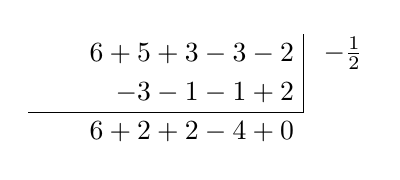
\begin{tikzpicture}
    \node at (0,0)[left]{$6+5+3-3-2$};
    \node at (0,-.5)[left]{$-3-1-1+2$};
    \node at (0,-1)[left]{$6+2+2-4+\boxed{0}$};
    \draw (-3.5,-.75)--(0,-.75)--(0,.25);
    \node at (.5,0){$-\frac{1}{2}$};
\end{tikzpicture}
\end{center}
所以$-\frac{1}{2}$是$f(x)$的根,由因式定理可得
\[f(x)=\left(x+\frac{1}{2}\right)(\poly{6,2,2,-4})\]

令$f_1(x)=\poly{6,2,2,-4}$,则$f(x)=\left(x+\frac{1}{2}\right)\cdot f_1(x)$

对$f_1(x)$求有理根,试除后知$f\left(\pm\frac{1}{3}\right)\ne 0$,因而$\pm\frac{1}{3}$不是$f_1(x)$的根,当然也不是$f(x)$的根,再用$\frac{2}{3}$试除:
\begin{center}
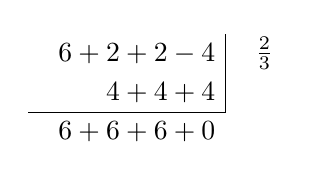
\begin{tikzpicture}
    \node at (0,0)[left]{$6+2+2-4$};
    \node at (0,-.5)[left]{$4+4+4$};
    \node at (0,-1)[left]{$6+6+6+\boxed{0}$};
    \draw (-2.5,-.75)--(0,-.75)--(0,.25);
    \node at (.5,0){$\frac{2}{3}$};
\end{tikzpicture}
\end{center}
所以$\frac{2}{3}$是$f_1(x)$的根,也就是$f(x)$的又一个根,因此
\[\begin{split}
    f(x)&=\left(x+\frac{1}{2}\right)\left(x-\frac{2}{3}\right)(\poly{6,6,6})\\
    &=6\left(x+\frac{1}{2}\right)\left(x-\frac{2}{3}\right)(\poly{1,1,1})
\end{split}\]

这里由于$x^2+x+1$的判别式$\Delta<0$, 因而它没有实数根,更不会有有理根,所以$f(2)$的有理根为$-\frac{1}{2}$, $\frac{2}{3}$.
\end{solution}

\begin{ex}
\begin{enumerate}
    \item 求$f(x)=6x^5+19x^4+22x^3+23x^2+16x+4$的有理根.
    \item 证明:多项式$f(x)=a_nx^n+a_{n-1}x^{n-1}+\cdots+a_1x+a_0$有根1的必要充分条件是
    \[ a_n+a_{n-1}+\cdots +a_1+a_0=0\]
\end{enumerate}
\end{ex}

\subsection{多项式的正根与负根}

对于实系数多项式
\[f(x)=a_nx^n+a_{n-1}x^{n-1}+\cdots+a_1x+a_0,\qquad (a_n\ne 0)\]
的根,我们有以下判定有、无正根或负根的定理:

\begin{blk}{定理3}
    如果实系数多项式
    \[f(x)=a_nx^n+a_{n-1}x^{n-1}+\cdots+a_1x+a_0,\qquad (a_n\ne 0)\]
    的各项系数$a_i,\; (i=n,n-1,\ldots,1, 0)$都是非负数,那么这个多项式$f(x)$就没有正数根.
\end{blk}

\begin{proof}
(用反证法)若$\alpha>0$且$f(\alpha)=0$, 则
\[a_n\alpha^n+a_{n-1}\alpha^{n-1}+\cdots+a_1\alpha+a_0=0\]

等号左边全是非负数,但由已知其中至少有首项系数不为零,所以它们的和不可能为零,而等号右边为零.这是不可能的.所以$f(\alpha)=0$不成立,即$f(x)$没有正根.

由于$-f(x)$与$f(x)$有完全相同的根,所以把“$a_n,a_{n-1},\ldots,a_1,a_0$全是非负数”改为“$a_n,a_{n-1},\ldots,a_1,a_0$全是非正数”,则结论不变.
\end{proof}

这样一来,如果要求一个各项系数符号统一的多项式的根,就可以不考虑正根了.如练习中的1肯定不会有正根.

\begin{blk}{定理4}
     如果实系数多项式
 \[f(x)=a_nx^n+a_{n-1}x^{n-1}+\cdots+a_1x+a_0,\qquad (a_n\ne 0)\]
偶次项系数都为非负(或非正)数,而奇次项系数又都为非正(或非负)数.那么这个多项式$f(x)$就没有负根.
\end{blk}

同学们可以自己用反证法证明这个定理.

有了这两个定理,配合定理1, 2就可以进一步缩小求有理根时试除的范围.

\begin{example}
    求$f(x)=5x^6-7x^5-8x^4-x^3+7x^2+8x+4$的有理根.
\end{example}

\begin{solution}
$f(x)$可能有的有理数根是$\pm 1,\pm 2,\pm 4,\pm \frac{1}{5},
\pm \frac{2}{5}, \pm \frac{4}{5}$.

用$x-1$试除得 $f(1)=0$, 因而有
\[f (x) = (x-1) (5x^5-2x^4-10x^3-11x^2-4x+4)=(x-1) f_1(x)\]
$f_1(x)$可能有的有理数根还是那几个,但再用$x-1$ 试除
$f_1(x)$, 不能整除,用$x-2$试除$f_1(x)$, 得$f_1(2)=0$, 因而有
\[f_1 (x) = (x-2) (5x^4+8x^3+6x^2+x-2)=(x-2)f_2(x)\]
$f_1(x)$所没有的根,$f_2(x)$当然也不会有.因此,$f_2(x)$可能有的有理数根是$-1,\pm 2,\pm \frac{1}{5},\pm \frac{2}{5}$. 但再用$x-2$试除$f_2(x)$不能整除,说明$f_2(x)$已没有正整数根;用$5x-1$试除$f_2(x)$不能整除,再用$5x-2$试除$f_2(x)$, 得$f_2\left(\frac{2}{5}\right)=0$, 
因而又有
\[f_2 (x) = (5x-2) (x^3+2x^2+2x+1)=(5x-2)f_3(x)\]
$f_3(x)$已没有正根,可能有的负根只是$x=-1$; 用$x+1$试除$f_3(x)$得$f_1(-1)=0$, 因而有
\[f_5 (x) = (x+1) (x^2+x+1)=(x+1)f_4(x)\]
$f_4(x)$已没有实数根,因而,说明$f(x)$不再有有理数根.所
以$f(x)$的有理数的是$1, 2,\frac{2}{5},-1$.
\end{solution}

\begin{ex}
\begin{enumerate}
    \item 求$f(x)=x^3-4x^2+x+6$的有理根.
    \item 解方程$2x^4+x^3+12=7x^2+16x$(仅求有理根).
\end{enumerate}
\end{ex}

\section*{习题4.2}
\addcontentsline{toc}{subsection}{习题4.2}
\begin{enumerate}
    \item 求下列多项式的有理根:
    \begin{multicols}{2}
  \begin{enumerate}
\item $x^3-7x+6$
\item $x^4-2x^2+3x-2$
\item $x^3-9x^2+26x-24$
\item $10x^3-9x^2-3x+2$
\item $2x^5-5x^2-2x+2$
\item $5x^4+24x^3-15x^2-118x+24$
\item $x^4-4a^3x+3a^4\quad (a\in\mathbb{Q})$
\item $x^3-ax^2-b^2x+ab^2\quad (a,b\in\mathbb{Q})$
\end{enumerate}      
    \end{multicols}
\item 分解因式:
\begin{enumerate}
    \item $6x^4+5x^3y+3x^2y^2-3xy^3-2y^4$
    \item $x^4-(a^2+b^2)x^2 +a^2b^2$
    \item $x^4-4x+3$
\end{enumerate}

\item 解下列方程:
\begin{enumerate}
    \item $4x^3-3x-1=0$
\item $8x^4-6x^3-7x^2+6x-1=0$
\end{enumerate}

\item 试证明:$-1$为多项式$f(x)$的根的必要充分条件是$f(x)$的奇次项系数之和等于$f(x)$的偶次项系数之和.

\item 证明:$f(x)=2x^3+2x-1$ 没有有理根.
\item 求$g(x)=2x^5+3x^4-15x^3-26x^2-27x-9$的有理根,并分解因式.
\end{enumerate}
    
\section{两个多项式的公根与多项式的重根}
公根和重根的问题,也是多项式理论中的基本问题,特别是多项式的重根问题,在下一节实根的讨论与计算中将起重要作用.

\subsection{两多项式的公根} 
设多项式$f(x)$与$g(x)$都有一个根$\alpha$, 即$f(\alpha )=0$, $g(\alpha )=0$, 则$\alpha$ 就叫做多项式$f(x)$与$g(x)$的公根.

由因式定理可以知道,多项式$f(x)$有一个根$\alpha$ 的充要条件是$f(x)$含有一次因式$x-\alpha$.

因此,对于两个多项式$f(x)$, $g(x)$的公根$\alpha$, 就有以下定理:

\begin{blk}{定理1}
    两多项式$f(x)$, $g(x)$有一个公根的必要充分条件是这两个多项式必有一个一次公因式.
\end{blk}

\begin{proof}
    必要性.设$f(x)$, $g(x)$有一个公根$\alpha$, 则由因式定理得
\[f (x) = (x-\alpha ) \cdot f_1 (x),\qquad g(x)=(x-\alpha )\cdot g (x)\]
显然,$f(x)$, $g(x)$有一次公因式 $x-\alpha$.

充分性.设$f(x)$, $g(x)$有一公因式$x-\alpha$, 则有
\[f (x) = (x-\alpha ) \cdot f_1 (x),\qquad g (x) = (x-\alpha ) \cdot g_1 (x)\]
显然就有$f(\alpha )=0$, $g(\alpha )=0$. 所以,
$\alpha$ 就是$f(x)$, $g(x)$的一个公根.

又由于两个多项式的公因式都是它们的最高公因式的因
式,因此,两多项式的公根必定都是它们的最高公因式的根.反之,两多项式的最高公因式的根也必定是这两个多项式的公根.

这样一来,要求两个多项式的公根,只要先求出它们的最高公因式,再求这一公因式的根就可以了.
\end{proof}

\begin{example}
    求$f(x)=2x^3+x^2-5x-3$与$g(x)=2x^3-5x^2+x+3$的公根.
\end{example}

\begin{solution}
    先用辗转相除法求得$\big(f (x) ,g (x) \big) =x^2-x-1$
    这一多项式的根为$a=1\pm\frac{\sqrt{5}}{2}$. 所以$f(x)$与$g(x)$的公根为
\[x_1=1+\frac{\sqrt{5}}{2},\qquad x_2=1-\frac{\sqrt{5}}{2}\]
    
    如果能通过确定每个多项式有理根的范围首先将多项式进行因式分解,那么也一样可以求得两多项式的公根,这样也就省去辗转相除求最高公因式的繁杂计算了.

    还可以先求出一个多项式的根,再去逐个代入另一多项式进行检验,凡能使第二个多项式的值为0的,就是公根;否则就不是.
\end{solution}

\begin{example}
    试求$f(x)=ax^2+bx+c$与$g(x)=x^2-1$有一个公根的必要条件.
\end{example}

\begin{solution}
    因为$g(x)=x^2-1=(x+1)(x-1)$, 所以
    $g(x)$有两个根$1,-1$, 因此,$f(x)$与$g(x)$有一个公根只可能是1或$-1$.

若公根为1, 则$a+b+c=0$;若公根为$-1$, 则$a-b+c=0$.所以$f(x)$与$g(x)$有一个公根的必要条件是
\[a+b+c=0\quad \text{或}\quad a-b+c=0\]
\end{solution}

\begin{ex}
    \begin{enumerate}
        \item 试求$f(x)=4x^4+26x^4+51x^3-7x-24$与
$g(x)=3x^4+20x^3+32x^2-8x-32$的公根.
\item 试求$f(x)=4x^5-5x^4+1$与$g(x)=x^4-4x+3$的公根.
\item 如果$f(x)=x^2+kx+1$与$g(x)=x^2+x+k$且$k\ne 1$,
并已知它们只有一个公根.试求$k$的值及这一公根的值.
    \end{enumerate}
\end{ex}

\subsection{多项式的重根}

对于多项式$f(x)$, 如果有$f(x)=(x-\alpha )^m\cdot q(x)$,且$q(\alpha )\ne 0,\; (m>1\in\mathbb{Z})$.
那么,我们就说$\alpha$ 是$f(x)$的$m$重根.

重根的判定和排除,是计算多项式的实数根时很注重的问题.在此,我们给出以下定理.

\begin{blk}{定理2}
    如果$\alpha$ 是多项式$f(x)$的$m$重根($m>1$),那么$\alpha$ 必定是$f'(x)$的$m-1$重根.
\end{blk}

\begin{proof}
    由定理条件知$f(x)=(x-\alpha )^m\cdot q(x)$且$q(\alpha )\ne 0$, 又由多项式乘积的求导数公式,得
\[\begin{split}
     f' (x) &=m (x-\alpha )^{m-1}\cdot q (x) + (x-\alpha )^m\cdot q'(x)\\
&=(x-\alpha ) ^{m-1}\cdot  [mq (x) + (x-\alpha ) q' (x) ]
\end{split}\]
其中由于$q(\alpha )\ne 0$, $m>1$, 因而$m\cdot q(\alpha )\ne 0$,所以$\alpha$ 就是$f'(x)$的$m-1$重根.
\end{proof}

\begin{blk}{定理3}
    $\alpha$ 是多项式$f(x)$的二重根的必要充分条件是$\alpha$ 为$f(x)$与$f'(x)$的公根,且$f''(\alpha )\ne 0$.
\end{blk}

\begin{proof}
    必要性:由泰勒公式,得
\begin{equation}
    f(x)=f(\alpha)+\frac{f'(\alpha)}{1!}(x-\alpha)+\frac{f''(\alpha)}{2!}(x-\alpha)^2+\cdots+\frac{f^{(n)}(\alpha)}{n!}(x-\alpha)^n
\end{equation}
由于$\alpha$ 是$f(x)$的二重根,根据因式定理,得
\[(x-\alpha )^2|f (x) \]
因而有:
$f (\alpha ) +\frac{f' (\alpha )}{1!} (x-\alpha )=0$.

所以,$f(\alpha )=f'(\alpha )=0$, 且$f''(\alpha )\ne 0$, $\alpha$ 是$f(x)$, $f'(x)$的公根,对任意$x$都成立.

充分性:由$f(x)$,$f'(x)$有公根$\alpha$, 且$f''(\alpha )\ne 0$,则$f(\alpha)= 0$,$f'(\alpha)=0$.再从泰勒公式(4.12)不难得出
\[(x-\alpha )^2|f (x) \]
所以,$\alpha$是$f(x)$的二重根.
\end{proof}

定理3完全可以类似地推广到m重根的情形,得到下述定理:

\begin{blk}{定理4}
    $\alpha$ 是$f(x)$的$m$重根的必要充分条件是$\alpha$ 是$f(x),f'(x),\ldots,f^{(m-1)}(x)$的公根,且$f^{(m)}(\alpha )\ne 0$.
\end{blk}

如果再结合定理1、2的内容,我们就可以得出:要判定
$f(x)$有没有重根,只要看$f'(x)$, $f(x)$的最高公因式就可以了,若最高公因式含有因式$(x-\alpha )^{m-1}$, 则可以断定$f(x)$有$m$重根$\alpha$, 同时还可以断定$f'(x)$有$m-1$重根$\alpha$, $f''(x)$有$m-2$重根$\alpha,\ldots$


\begin{example}
    试求$f(x)=\poly{1,-3,2,2,-3,1}$的重根.
\end{example}

\begin{solution}
    先求出导数$f' (x) =5x^4-12x^3+6x^2+4x-3$,
再用辗转相除法求出
\[\big(f (x) ,f' (x) \big) =x^3-3x^2+3x-1= (x-1)^3\]
所以,
\[(x-1)^3|f(x),\qquad (x-1)|f'(x)\]
即$x=1$是$f(x)$与$f'(x)$的公根.因此,$f(x)$有重根1(而且是$f(x)$的4重根,$f'(x)$的3重根).
\end{solution}

\begin{example}
  求证方程$x^4+2x^3-15x^2+4x+20=0$
有二重根,并求出这个方程的根.  
\end{example}

\begin{solution}
 设$f(x)=x^4+2x^3-15x^2+4x+20,\quad 
f' (x) =4x^3+6x^2-30x+4$,
由辗转相除法可求出$\big(f(x),f'(x)\big)=x-2$, 这是一次式.
所以,$f(x)$有二重根2, 也就是原方程有二重根2, 再用因式定理,得:
\[f (x) = (x-2)^2  (x^2+6x+5)= (x-2)^2 (x+1)(x+5)\]
因此,原方程可变形为
\[(x-2)^2 (x+1)(x+5)=0\]
所以原方程的各根为:$2, 2,-1,-5$.   
\end{solution}

\begin{ex}
    \begin{enumerate}
        \item 判定下列多项式是否有重根?若有,试求出重根来:
\begin{enumerate}
    \item $f(x)=\poly{1,-4,0,8,4}$
    \item $g(x)=\poly{4,8,-8,3}$
\end{enumerate}
        \item 举例说明定理2的逆命题是不正确的.
    \end{enumerate}
\end{ex}

\section*{习题4.3}
\addcontentsline{toc}{subsection}{习题4.3}
\begin{enumerate}
\item 求下列各组多项式的公根:
\begin{enumerate}
    \item $f (x) =x^3+5x^2+3x-9,\qquad 
g (x) =x^3+7x^2+15x+9$
\item $f (x) =x^3+3x^2-2x-6,\qquad 
g (x) =x^3-3x^2-2x+6$
\item  $f (x) =x^4-5x^2+4,\qquad g (x) =x^2+x-2$
\end{enumerate}


\item 已知$f(x)=2x^2-(3m+2)x+12$与$g(x)=4x^2-(9m-2)x+36$有一个公根,试求$m$的值.
\item 求下列多项式的重根:
\begin{enumerate}
    \item $f (x) =9x^3+12x^2-11x+2$
    \item $f(x)=\poly{1,0,4,-4,-3}$
    \item $f (x) =x^4-2x^3-x^2-4x+12$
    \item $g (x) =x^5-5x^4+7x^3-2x^2+4x-8$
\end{enumerate}

\item 若多项式$f(x)=x^3-12x+a$有重根,试求$a$.
\item 试求多项式$g(x)=x^4-px^2+q$有重根的必要条件
\item 已知多项式$f(x)=\poly{1,-1,-3,4,-4}$有两个互为相
反数的根,试求出这两个根.
\item 试一试,举例验证:如果多项式$f(x)$有重根,那么多
项式$g(x)=\frac{f(x)}{\bigl(f (x) ,f' (x)\bigr)}$就没有重根,但$g(x)$与$f(x)$
有相同的根.
\end{enumerate}


\section{实系数多项式的实数根}
对于实系数多项式
\[f(x)=a_nx^n+a_{n-1}x^{n-1}+\cdots+a_1x+a_0,\qquad (a_n\ne 0)\]
的根的讨论,要困难和复杂得多,因为多项式的根除了有理根之外,更多的是存在无理数根,而且五次以上的多项式,求根公式根本没有.因此,如何求出这些多项式的实根(如果存在的话)?特别是如何求出这些多项式的无理根的近似值?就成为我们急需讨论的内容了.

\subsection{计算实根近似值的基本思想}
求实系数多项式的实
根的近似值,主要采用逼近法,其理论根据就是今后要详细学习的中间值定理,我们现在叙述和解释如下:

\begin{blk}{定理1(中间值定理)}
    $f(x)$是一个实系数的多项式,$a<b$.若$f(a)$
    与$f(b)$符号相反,则一定存在一实数$c$,$a<c<b$使$f(c)=0$.
\end{blk}

我们从图象上来解释中间值定理.如图4.1, 由于$f(a)$
与$f(b)$符号相反,所以点$\big(a,f(a)\big)$及点$\big(b,f(b)\big)$分别在$x$轴的两侧,而曲线$y=f(x)$是连续的.因此它从$x$轴的一侧运动到$x$轴的另一侧,至少要“穿过”$x$轴一次.若在$(c,0)$点穿过,就有$f(c)=0$.

\begin{figure}[htp]
    \centering
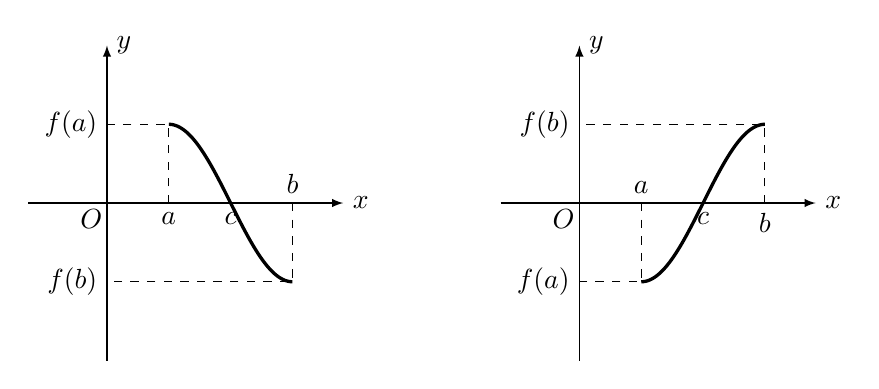
\begin{tikzpicture}[>=latex]
\begin{scope}
    \draw[->] (-1,0)--(3,0)node[right]{$x$};
    \draw[->] (0,-2)--(0,2)node[right]{$y$};
\draw [domain=pi/4:.75*pi, samples=100, very thick]plot(\x, {sin(2*\x r)});
\draw[dashed] (pi/4,0)node[below]{$a$}--(pi/4,1)--(0,1)node[left]{$f(a)$};
\draw[dashed] (.75*pi,0)node[above]{$b$}--(.75*pi,-1)--(0,-1)node[left]{$f(b)$};
\node at (-.2,-.2){$O$};
\node at (.5*pi,0)[below]{$c$};
\end{scope}
\begin{scope}[xshift=6cm]
    \draw[->] (-1,0)--(3,0)node[right]{$x$};
    \draw[->] (0,-2)--(0,2)node[right]{$y$};
\draw [domain=pi/4:.75*pi, samples=100, very thick]plot(\x, {-sin(2*\x r)});
\draw[dashed] (pi/4,0)node[above]{$a$}--(pi/4,-1)--(0,-1)node[left]{$f(a)$};
\draw[dashed] (.75*pi,0)node[below]{$b$}--(.75*pi,1)--(0,1)node[left]{$f(b)$};
\node at (-.2,-.2){$O$};
\node at (.5*pi,0)[below]{$c$};
\end{scope}
\end{tikzpicture}
    \caption{}
\end{figure}

这样的解释尽管是直观形象的,但还不能算是严格证明.因为:什么叫连续?为什么多项式函数在$(-\infty,+\infty)$是连续的?这些问题还没有确切的交待过.而且对于一般连续函数的这一中间值定理,我们也不满足于仅仅是几何解释.不过我们目前只是直观承认这一条定理的内容并初步应用它.以后在微积分学习中再详细证明.

\begin{example}
    判断多项式$f(x)=\poly{1,0,-3,1}$的实根介于哪些连续整数之间?
\end{example}

\begin{solution}
显然,当$x\le -3$时,$f(x)<0$, 且有:
\[f (-2) =-1,\qquad f (-1) =+8,\qquad f (0) =+1,\qquad f (1)=-1,\qquad f(2)=+3\]

$x>3$时,$f(x)>0$.

所以$f(x)$在$(-2,-1)$, $(0, 1)$及$(1, 2)$各有一实根.
\end{solution}
    
例4.14说明了中间定理的作用,但并没有告诉我们多项式实根如何定位的基本方法.因为尽管在这一题中,$f(-2)$, $f(-1)$, $f(0)$, $f(1)$, $f(2)$求出后,实根的位置是显然的,但是怎样想到用$-2,-1, 0, 1, 2$的函数值作为试探的目标呢?万一$f(x)$的根是一个很大的数,例如$10^6$左右的数时,岂不要试上$10^6$个函数值?万一$f(x)$只有一个实数根,再找另两个根时不仅徒劳,而且不知到什么时候才能明确另两个不是实根.何况还可能有一些多项式根本没有实根.

这样看来,要寻求求多项式实根近似值的更完善的途径,必须解决以下三个问题:
\begin{enumerate}
\item 确定根的界限——求出一个区间,使多项式的实根在
这一范围内;    
\item 根的分离定位——判定多项式的实根的个数,并使每
个实根只包含在一个小区间内;    
\item 根的计算——求出每一实根的近似值.
\end{enumerate}

本节将系统解决这些问题,在着手解决这些问题之前,我们首先要明确逼近法的基本思想,即如何计算出$f(x)$在$(a,b)$中的一个实根的近似值?使它能达到指定的精确度?

\begin{example}
    求$f(2)=x^3-3x+1$在$(1, 2)$中的实根的近似值.(要求误差不超过0.001)
\end{example}

\begin{solution}
    由中间值定理可知,在$(1, 2)$中$f(x)$有一个实根,设为$\alpha$,为了求出要求精度范围内的近似值,可以把区间$(1, 2)$十等分,将分点$1.1,\; 1.2,\ldots,\; 1.8,\; 1.9$分别代入$f(x)$, 由于$f(1. 5)=-0.125$, $f(1. 6)=+0.296$, 所以这个根$\alpha$在$(1.5, 1. 6)$中,即$\alpha$精确到0.1的不足近似值为1.5.
    
    再把区间$(1.5, 1. 6)$十等分,将分点$1.51,\; 1.52,\ldots,\; 1.58, 1.59$分别代入$f(x)$, 因为$f(1.53)=-0.008423$, $f(1.54)=+0.03226$,所以这个根$\alpha$在$(1.53, 1. 54)$中,即$\alpha$精确到0.01的不足近似值为1.53.

    继续将$(1.53, 1.54)$十等分,计算各分点的多项式的值,因为$f(1. 532)=-0. 00010$, $f(1. 533)=+0.00369$, 所以,根$\alpha$在$(1. 532, 1. 533)$中,它的精确到0.001的不足近似值为$\alpha\approx1.532$.

    如果继续这样做下去,只要细心、不嫌繁,就可以求出
    精确到任意水平的根的近似值.
\end{solution}

    例4.15说明是逼近法的基本思想,也是求实根的基本方法,它的主要依据就是中间值定理.但方法繁,计算量大,现在已有不少更先进的算法,我们将在后边介绍一种改进了的方法.

\begin{ex}
\begin{enumerate}
    \item 利用中间值定理,判定下列多项式的实根在哪些连续整
数之间:
\begin{enumerate}
    \item $f (x) =x^4-6x^3+5x^2+12x-6$
    \item $f (x) =2x^3-5x^2+5x-3$
\end{enumerate}
\item 利用逼近法,试求$f(x)=x^3-8x+1$在$(0, 1)$中的实
根,(精确到0.001)
\end{enumerate}
\end{ex}

\subsection{实系数多项式实根的界和定位}

我们已经知道,根
据中间值定理,可以经过耐心细致的计算,首先确定多项式实根的位置在哪些连续整数之间,其次再用逼近法去求每一个实根的近似值.但是,对某一些多项式,如果我们一开
始就用一个整数进行试算,可能会发生困难,一则难在应从哪一个整数试起呢?二则难在有些多项式用整数试算找不到实根存在的区间,中间值定理无能为力.

\begin{example}
   试判定下列多式项的实根在哪两个连续整数之间?
\begin{multicols}{2}
 \begin{enumerate}
     \item $f (x) =x^4-6x^2+10$
     \item $g(x)=8x^2-8x+1$
 \end{enumerate}
\end{multicols}
\end{example}

\begin{solution}
\begin{enumerate}
    \item 由于$f(x)=(x^2-3)^2+1$, 因此,无论用那一个整数$a$去试算,恒有$f(a)>0$, 中间值定理无法判断.
    
    实际上,$f(x)$确实没有实根.
    \item 一方面当我们用一个个
    整数$a$试算$g(a)$的值时,会发现总有$g(a)>0$, 好像可以断言$g(x)$没有实根了;但另一方面,
    用求根公式可以求得$g(x)$的两个根:
    $x=\frac{2\pm\sqrt{2}}{4}$,
    显然都是实根.只不过这两个实根都在$(0, 1)$中间,其图象如图4.2所示.

    这样看来,尽管$g(0)>0$, $g(1)>0$是同号的,但在$(0, 1)$中不是没有实根,而是有两个实根.
\end{enumerate}

\begin{figure}[htp]
    \centering
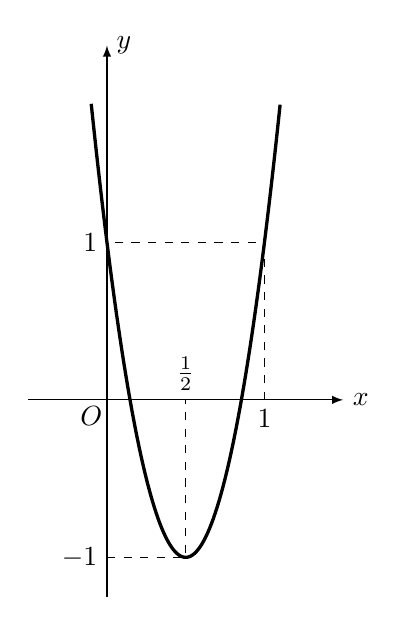
\begin{tikzpicture}[>=latex, scale=2]
\draw[->] (-.5,0)--(1.5,0)node[right]{$x$};
\draw[->] (0,-1.25)--(0,2.25)node[right]{$y$};
\node at (-.1,-.1){$O$};
\draw[domain=-.1:1.1, samples=100, very thick]plot(\x, {8*\x*\x-8*\x+1});
\draw [dashed](0,-1)node[left]{$-1$}--(.5,-1)--(.5,0)node[above]{$\frac{1}{2}$};
\draw [dashed](1,0)node[below]{$1$}--(1,1)--(0,1)node[left]{1};

\end{tikzpicture}
    \caption{}
\end{figure}
\end{solution}

这就提醒我们注意,中间值定理所述的内容中$f(a)$与$f(b)$符号相反只是$f(x)$在$(a,b)$中有实根的充分条件,但不是必要条件.
    
    依据中间值定理,运用逼近法求多项式的实根时,由于会遇到以上困难,因而我们就不得不进一步来探求新的更有效的方法.史笃姆方法就是彻底解决实根个数及定位的有效方法.
    
    史笃姆方法只是对没有重根的多项式来说的,因此可设多项式$f(x)$没有重根.

又因为当多项式的首项系数$a_n\ne 1$时,可用$a_n$去除这
个多项式的每一项,从而得到一个首项系数为1的实系数多项式,它的零点(实根)不发生变化.因此,我们就可设
$f (x) =x^n+a_{n-1}x^{n-1}+\cdots +a_1x +a_0$是一个没有重根的实系数多项式.

\subsubsection{$f(x)$的根界}

可以证明,$f(x)$的每一个根的绝对值都不会大于$f(x)$的各项系数绝对值的和.因此,我们可取
\[M=1+|a_{n-1}|+|a_{n-2}|+\cdots+|a_1|+|a_0|\]
作为$f(x)$的根界.即$f(x)$的所有实根都在区间$[-M,M]$中.这里我们不加证明而引用这一结论.

\begin{example}
    写出多项式$\varphi(x)=x^3-10x+2$ 的根界.
\end{example}

\begin{solution}
 $\because\quad    M=1+|-10|+2=13$
 
 $\therefore\quad \varphi(x)$的所有根都在区间$[-13, 13]$之内.
\end{solution}

\subsubsection{史笃姆函数序列}
设没有重根的多项式$f(x)$和它的导数$f'(x)$, 则有${\rm deg}f(x)={\rm deg}f'(x)+1$, 把$f'(x)$记为$f_1(x)$, 并作带余除法,得
\[f (x) =q_1 (x)\cdot f_1(x)+r_1(x)\]

其中$r_1(x)=0$或$r_1(x)\ne 0$,${\rm deg}r_1(x)<{\rm deg}f_1(x)$.
在这里只有$f(x)$是一次多项式,从而$f_1(x)$是零次多项式时,才能有$r_1(x)=0$, 否则$r_1(x)$不会等于零.记$f_2(x)=-r_1(x)$,(注意,式中的一个负号十分重要).

又以$f_2(x)$除$f_1(x)$, 得$f_1(x)=q_2(x)f_2(x)+r_2(x)$, 同样,只有$f_2(x)$是零次多项式时,才有$r_2(x)=0$, 否则$r_2(x)\ne 0$, 记$f_3(x)=-r_2(x)$. 如此继续下来,直到可以整除为止.即得
\[\begin{split}
    f(x)&=q_1(x)f_1(x)-f_2(x)\\
    f_1(x)&=q_2(x)f_2(x)-f_3(x)\\
    f_2(x)&=q_3(x)f_3(x)-f_4(x)\\
    \cdots &\cdots \cdots \cdots \cdots \\
    f_{k-1}(x)&=q_k(x)f_k(x)-f_{k+1}(x)\\
    \cdots &\cdots \cdots \cdots \cdots \\
    f_{s-1}(x)&=q_s(x)f_s(x)\\
\end{split}\]

容易看到,这些计算实际上是对两个多项式$f(x)$及$f'(x)$进行辗转相除,只不过每一次的余式改变一个符号而已.由于非零数因子不影响辗转相除的结果,所以最后能整除的除式$f_s(x)$就是$f(x)$与$f'(x)$的最高公因式.但是我们己给出$f(x)$没有重根这样一个条件,所以$f_s(x)$只能是零次多项式,因而可记为$f_s$.
\[f (x) ,f_1 (x) ,f_2 (x),\ldots,f_k(x),\ldots,f_s\]
叫做多项式$f(x)$的\textbf{史笃姆函数序列}.


\begin{example}
    试求$f(x)=\poly{1,0,-10,2}$的史笃姆函数序列.
\end{example}

\begin{solution}
\[f_1(x)=f'(x)=3x^2-10\]
用$f_1(x)$除$f(x)$,得:
\[r_1(x)=-\frac{20}{3}x+2\]
$\therefore\quad f_2(x)=-r_1(x)=\frac{20}{3}x-2=\frac{20}{3}\left(x-\frac{3}{10}\right)$

用$f_2(x)$除$f_1(x)$,得:$r_2(x)=-\frac{973}{100}$

$\therefore\quad f_3=\frac{973}{100}$    

因此,所求的史笃姆函数序列为:
\[x^3-10x-2,\quad 3x^2-10,\quad \frac{20}{3}\left(x-\frac{3}{10}\right),\quad \frac{973}{100}\]
\end{solution}

由于以下讨论史笃姆函数序列时,只考虑$x$取某一数值时,$f_k(x)$为零,为正还是为负,所以在任一个史笃姆函数列中,乘以一个正常数(注意必须是正的)不影响讨论结果.因此对于上述例题所得的史笃姆函数序列,可以写成:
\[\begin{split}
    f (x) &=x^3-10x+2\\
    f_1 (x) &=3x^2-10\\
    f_2 (x) &=10x-3\\
    f_3&=1
\end{split}\]
对讨论结果不会有影响.

\subsubsection{实数列的变号数}

在史笃姆函数序列中,以实数$a$代$x$, 得到一系列实常数:$$f(a),f_1(a),f_2(a),\ldots,f_k(a),\ldots, f_s$$ 这些数有正、有负,也可能有零.丢开那些具体数字,只考查各项的符号,就成为一系列符号的排列,例如
\begin{equation}
    +\quad +\quad +\quad -\quad -\quad +\quad -\quad -\quad +\quad -\quad +\quad -\quad -\quad +
\end{equation}

如果在这个排列中,两个相邻的符号相反,我们就说这一排列有一个变号.整个排列中变号的总数,就叫做它的变号数.(4.13)的变号数是6.

如果在实数列中含有零,那么,它的变号数就指去掉零以后,剩下的各数组成的数列的变号数.例如
\begin{equation}
    +\quad +\quad -\quad 0\quad +\quad +\quad 0\quad +\quad -\quad +\quad -\quad -
\end{equation}
的变号数,就是指
\begin{equation}
    +\quad +\quad -\quad +\quad +\quad +\quad -\quad +\quad -\quad -
\end{equation}
的变号数,显然它们的变号数是5.

给出一个多项式的史笃姆函数序列以后,用实数$a$代入,得实数列
\[f (a) ,f_1 (a) ,f_2 (a) , \ldots,f_k (a) , \ldots,f_s\] 
我们把这一数列的变号的个数记为$W(a)$.

\subsubsection{史笃姆定理及其证明}

\begin{blk}{定理2(史笃姆定理)}
    如果用$-M$, $M$代入没有重根的多项式$f(x)$的史笃姆函数序列,所得实数列的变号数分别为$W(-M)$与$W(M)$, 那么,多项式$f(x)$在$[-M,M]$内就有$W(-M)-W(M)$个实根.
\end{blk}

\begin{example}
求多项式
$f (x) =x^3-10x+2$
的实根个数及各个根所在的位置.
\end{example}

\begin{solution}
    由例4.17知$f(a)$的根都在$[-13, 13]$之内,
    又由例4.18知$f(x)$的史笃姆函数序列为
\[f (x) =x^3-10x+2,\quad f_1(x) =3x^2-10,\quad f_2 (x) =10x-8,\quad f_3=1\]
在根界$[-13,+13]$内,取点计算变号数,变号的情况列表如下:
\begin{center}
    \begin{tabular}{cccccc}
$x$ & $f(x)$ & $f_1(x)$ & $f_2(x)$ & $f_3$ & $W(x)$\\
$-13$ & $-$ &$+$ & $-$ &$+$&3\\
$-4$ & $-$ &$+$ & $-$ &$+$&3\\
$-3$ & $+$ &$+$ & $-$ &$+$&2\\
$-2$ & $+$ &$+$ & $-$ &$+$&2\\
$-1$ & $+$ &$-$ & $-$ &$+$&2\\
$0$ & $+$ &$-$ & $-$ &$+$&2\\
$1$ & $-$ &$-$ & $+$ &$+$&1\\
$2$ & $-$ &$+$ & $+$ &$+$&1\\
$3$ & $-$ &$+$ & $+$ &$+$&1\\
$4$ & $+$ &$+$ & $+$ &$+$&0\\
$+13$ & $+$ &$+$ & $+$ &$+$&0\\
    \end{tabular}
\end{center}
从中根据史笃姆定理就可以断定,多项式$f(x)=x^3-10x+2$共有$W(-13)-W(13)=8$个实根;同时还可以进一步得出,这三个实根分别在$(-4,-3)$, $(0, 1)$, $(3, 4)$三个区间之中.
\end{solution}

以下我们分几个步骤来证明史笃姆定理.(以下供选学)

第一个问题:会不会出现类似以下的排列
\[+\quad +\quad +\quad 0\quad +\quad +\quad -\]
即中间有一个零,而其左右同号,如果有这种情况,这个零就不能随便算作正的或负的了.
我们来证明这种情况不会产生,即:
\begin{blk}{}
   史笃姆函数序列中以一个实常数代入,居中间出
现一个零,则其左右必为一正一负,既不会出现相邻的两个零,也不会在零的左右出现两个同是正号或两个同是负号. 
\end{blk}


\begin{proof}
若以$a$代入$f_k(x)$, 得$f_k(a)$为零,则$(x-a) |f_k (x)$.

此时如果又有$f_{k+1}(x)=0$, 即 $(x-a) |f_{k+1} (x)$,则$x-a$为$f_k(x)$与$f_{k+1}(x)$的公因式,由此可知$x-a$也是$f(x)$与$f'(x)$的公因式,因而$a$是$f(x)$的重根,这与假设矛盾.所以$f_{k+1}(a)\ne 0$. 同理$f_{k-1}(a)\ne 0$.

又因为$$f_{k-1}(x)=q_k(x)f_k(x)-f_{k+1}(x)$$所以$$f_{k-1}(a)=q_k(a)f_k(a)-f_{k+1}(a)$$
现在$f_k(a)=0$,所以必然有$$f_{k-1}(a)=-f_{k+1}(x)$$
如果在运算过程中,$f_{k-1}(x)$, $f_{k+1}(x)$乘过不同的正常数,可能使$f_{k+1}(x)$与$f_{k-1}(a)$的绝对值不等,但符号总是相反的.可见一个零的左右的两个符号必相反.
\end{proof}

第二个问题:怎么会产生变号个数的变化?当$x$经过某一个$f_k(x)$的根而不是$f(x)$的根时,变号的个数会不会有变化?

变号数的变化来源于各个符号的变化.若$x$由$a$渐增到$b$, 完全没有经过$f(x)$及$f_k(x)$的任一个根(如例4.19中$x$由$-3$增加到$-2$, 或由$-1$增加到0, 或由2增加到3),则所有的符号都没有变,因而变号个数也不会变.

关于$x$通过$f_k(x)$的某一个根,但不是$f(x)$的根的情况,我们来证明:
\begin{blk}{}
    若$x$通过$f_k(x)$的某一个根,但不是$f(x)$的根时,史
笃姆函数序列的值只改变变号的位置,不改变变号的个数.
\end{blk}

如在例4.19中:$x$从$-2$到$-1$通过$f_1(x)$的根,史笃姆函数序列的值的符号,就从
\[+\quad +\quad -\quad +\]
改变为
\[+\quad -\quad -\quad +\]

变号的位置从第2到第3改变为从第1到第2; 但变号的个数仍是2.

\begin{proof}
    $f_k(x)$与$f_{k+1}(x)$没有公共的根,设$\alpha$是$f_k(x)$的一
个根,则$f_{k-1}(\alpha )\ne 0$, $f_{k+1}(\alpha )\ne 0$. 我们考虑$x$从$\alpha -\varepsilon$ 经过$\alpha$ 变到$\alpha +\varepsilon$ 的过程,$\varepsilon$取得如此之小,以至$f_{k-1}(x)$, $f_{k+1}(x)$都没有一个根在$(\alpha -\varepsilon ,\alpha +\varepsilon )$内,由中间值定理这总是可行的.

$f_k(\alpha )=0$, 已证明$f_{k-1}(\alpha )$与$f_{k-2}(\alpha)$异号,因此可能有下列四种情况:

\begin{center}
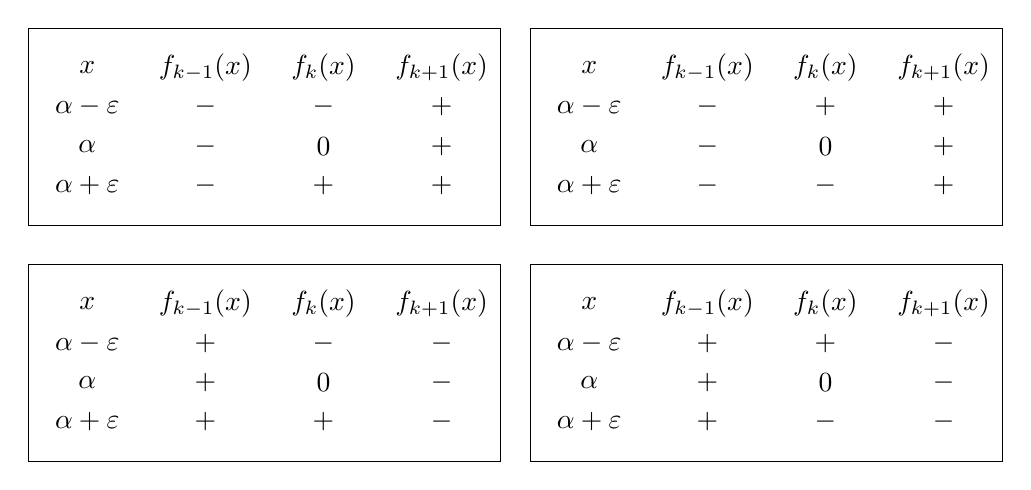
\begin{tikzpicture}[xscale=1.5]
\begin{scope}
    \foreach \x/\xtext in {1/x,2/f_{k-1}(x),3/f_{k}(x),4/f_{k+1}(x)}
    {
        \node at (\x,3){$\xtext$};
    }
    \foreach \x/\xtext in {1/\alpha-\varepsilon,2/-,3/-,4/+}
    {
        \node at (\x,2.5){$\xtext$};
    }
    \foreach \x/\xtext in {1/\alpha,2/-,3/0,4/+}
    {
        \node at (\x,2){$\xtext$};
    }
    \foreach \x/\xtext in {1/\alpha+\varepsilon,2/-,3/+,4/+}
    {
        \node at (\x,1.5){$\xtext$};
    }
    \draw (0.5,1) rectangle (4.5,3.5);
\end{scope}

\begin{scope}[xshift=4.25cm]
    \foreach \x/\xtext in {1/x,2/f_{k-1}(x),3/f_{k}(x),4/f_{k+1}(x)}
    {
        \node at (\x,3){$\xtext$};
    }
    \foreach \x/\xtext in {1/\alpha-\varepsilon,2/-,3/+,4/+}
    {
        \node at (\x,2.5){$\xtext$};
    }
    \foreach \x/\xtext in {1/\alpha,2/-,3/0,4/+}
    {
        \node at (\x,2){$\xtext$};
    }
    \foreach \x/\xtext in {1/\alpha+\varepsilon,2/-,3/-,4/+}
    {
        \node at (\x,1.5){$\xtext$};
    }
    \draw (0.5,1) rectangle (4.5,3.5);
\end{scope}

\begin{scope}[yshift=-3cm]
    \foreach \x/\xtext in {1/x,2/f_{k-1}(x),3/f_{k}(x),4/f_{k+1}(x)}
    {
        \node at (\x,3){$\xtext$};
    }
    \foreach \x/\xtext in {1/\alpha-\varepsilon,2/+,3/-,4/-}
    {
        \node at (\x,2.5){$\xtext$};
    }
    \foreach \x/\xtext in {1/\alpha,2/+,3/0,4/-}
    {
        \node at (\x,2){$\xtext$};
    }
    \foreach \x/\xtext in {1/\alpha+\varepsilon,2/+,3/+,4/-}
    {
        \node at (\x,1.5){$\xtext$};
    }
    \draw (0.5,1) rectangle (4.5,3.5);
\end{scope}

\begin{scope}[xshift=4.25cm, yshift=-3cm]
    \foreach \x/\xtext in {1/x,2/f_{k-1}(x),3/f_{k}(x),4/f_{k+1}(x)}
    {
        \node at (\x,3){$\xtext$};
    }
    \foreach \x/\xtext in {1/\alpha-\varepsilon,2/+,3/+,4/-}
    {
        \node at (\x,2.5){$\xtext$};
    }
    \foreach \x/\xtext in {1/\alpha,2/+,3/0,4/-}
    {
        \node at (\x,2){$\xtext$};
    }
    \foreach \x/\xtext in {1/\alpha+\varepsilon,2/+,3/-,4/-}
    {
        \node at (\x,1.5){$\xtext$};
    }
    \draw (0.5,1) rectangle (4.5,3.5);
\end{scope}
\end{tikzpicture}
\end{center}

可以看到,在任何一种情况下,史笃姆函数序列只改变变号的位置,不改变变号的个数.
\end{proof}

第三个问题:至此产生变号个数起变化的其他可能都已排除,那就只有一个可能会改变变号个数:$x$经过$f(x)$的根.因此我们就问:$x$从小到大渐增地变化,每经过$f(x)$的一个根时,变号的个数如何变化呢?以下就解决并证明这一问题.

\begin{blk}{}
$x$从小到大渐地增变化,每通过$f(x)$的一个根时,
史笃姆函数序列的值的变号就减少一个.
\end{blk}

\begin{proof}
我们只在$f(x)$的根$\alpha$邻近的一个区域$(\alpha-\varepsilon,\alpha+\varepsilon)$内考虑$f(x)$及$f_1(x)$(即$f'(x)$)的局部性质.因为$f(x)=0$, 
则$f'(x)\ne 0$. 我们取足够小的$\varepsilon$, 使$f'(x)$在$(\alpha-\varepsilon,\alpha+\varepsilon)$内符号不变:$f'(x)>0$时,$f(x)$递增,这说明$f(x)$由负变正;反之,$f'(x)<0$时,$f(x)$递减,说明$f(x)$由正变负.情况列表如下:
\begin{center}
    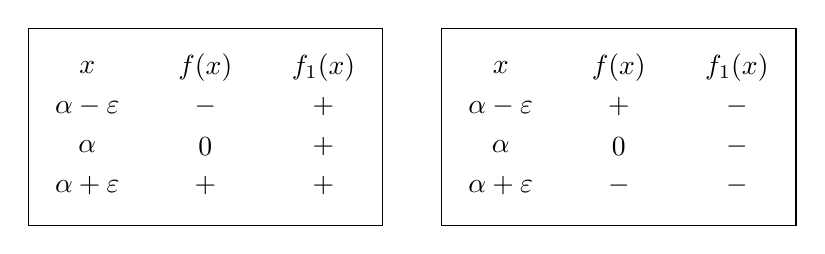
\begin{tikzpicture}[xscale=1.5]
    \begin{scope}
        \foreach \x/\xtext in {1/x,2/f(x),3/f_1(x)}
        {
            \node at (\x,3){$\xtext$};
        }
        \foreach \x/\xtext in {1/\alpha-\varepsilon,2/-,3/+}
        {
            \node at (\x,2.5){$\xtext$};
        }
        \foreach \x/\xtext in {1/\alpha,2/0,3/+}
        {
            \node at (\x,2){$\xtext$};
        }
        \foreach \x/\xtext in {1/\alpha+\varepsilon,2/+,3/+}
        {
            \node at (\x,1.5){$\xtext$};
        }
        \draw (0.5,1) rectangle (3.5,3.5);
    \end{scope}
    
    \begin{scope}[xshift=3.5cm]
        \foreach \x/\xtext in {1/x,2/f(x),3/f_1(x)}
        {
            \node at (\x,3){$\xtext$};
        }
        \foreach \x/\xtext in {1/\alpha-\varepsilon,2/+,3/-}
        {
            \node at (\x,2.5){$\xtext$};
        }
        \foreach \x/\xtext in {1/\alpha,2/0,3/-}
        {
            \node at (\x,2){$\xtext$};
        }
        \foreach \x/\xtext in {1/\alpha+\varepsilon,2/-,3/-}
        {
            \node at (\x,1.5){$\xtext$};
        }
        \draw (0.5,1) rectangle (3.5,3.5);
    \end{scope}
    \end{tikzpicture}
    \end{center}

可见在任何情况下,x从小做大每经过$f(x)$的一个根,史笃姆函数序列的值总是减少一个变号.
\end{proof}

综合以上三条,史笃姆定理即获证.

我们在叙述求实多项式实根位置的史笃姆方法及证明史笃姆定理时都强调这样一个假设:实多项式$f(x)$没有重根.对于这个条件的限制在应用上和理论上都会使我们感到不满足.从应用上说,是否在使用史笃姆方法以前要验证$f(x)$有没有重根?从理论上说,如果$f(x)$有重根,史笃姆定理会受到些什么损害?

我们来回答这两个问题.

第一,从应用上说,这个条件完全不会增加我们的计算量.因为求史笃姆函数序列的过程实际是用辗转相除法求$f(x)$及$f'(x)$的最高公因式过程.如果$f(x)$有重根,在上述运算中必然会看出.发现重根以后,我们把有关因式除掉(这些因式为零时的值就是$f(x)$的重根),再研究其没有重根部分的因式.这时,多项式的次数至少降低二次,对运算更有利.

第二,从理论上讲,如果有重根,史笃姆定理的结论同样正确,不过这时$f_s(x)$是一个次数不小于1的多项式,不可以写成$f_s'$而计算根的个数的时候,重根$\alpha$不论是多少重根,只作为1个根计数.即史笃姆函数序列的值在$x$由小到大经过$f(x)$的$m$重根$\alpha$时,变号数不是减少$m$个,而是只减少1个.我们不另作详细证明,只举以下一例说明.

\begin{example}
求多项式
\[f(x)=\poly{1,-1,-2,2,1,-1}=(x-1)^3(x+1)^2\]
的史笃姆函数序列中变号的变化情况.
\end{example}

\begin{solution}
先求$f(x)$的史笃姆序列及根界
\[\begin{split}
    f_1(x)&=\poly{5,-4,-6,4,1}=(x-1)^2(x+1)(5x+1)\\
    f_2(x)&=\poly{1,-1,-1,1}=(x-1)^2(x+1)\\
    f_3(x)&=0
\end{split}
    \]
根界:$M=8$,$\qquad \therefore\quad f(x)$的根在$[-8,+8]$中.变号情况列表如下:
\begin{center}
    \begin{tabular}{ccccc}
$x$ & $f(x)$ & $f_1(x)$ & $f_2(x)$ &  $W(x)$\\
$-8$ & $-$ & $+$ &$-$&2\\
$-2$ &$-$ & $+$ &$-$&2\\
$0$ & $-$ & $+$ &$+$&1\\
$2$ &  $+$ & $+$ &$+$&0\\
$+8$ &  $+$ & $+$ &$+$&0\\
    \end{tabular}
\end{center}

可知$f(x)$在$(-2, 0)$有一个根.(实际是二重根$-1$);在$(0, 2)$有一个根,(实际是三重根1).
\end{solution}

综上所述,我们可以看到史笃姆定理可以彻底地解决实系数多项式的实根的个数、定位等问题.因而,史笃姆定理也被称为实数范围内的代数基本定理.

\begin{ex}
\begin{enumerate}
    \item 试求多项式 $f(x)=x^3+3x^2-4x+1$ 的实根界、实根个数及各个实根的位置.
    \item 用史笃姆定理证明:$n$次多项式$f(x)$的实根个数不大于$n$.
\end{enumerate}
\end{ex}

\subsection{实系数多项式实根的计算}

在前面我们已经根据中间值定理,运用逼近方法求过的实根的近似值,但太繁,计算量也很大,以下我们将利用两种换元变形,改进计算过程,从而得到多项式实根近似计算的秦九韶方法.

\subsubsection{多项式的两种换元变形}

第一种变形:令$y=x-k$, 则$x=y+k$, 于是
\[\begin{split}
    f(x)&=f(k)+\frac{f'(k)}{1!}(x-k)+\frac{f''(k)}{2!}(x-k)^2+\cdots +\frac{f^{(n)}(k)}{n!}(x-k)^n\\
    &=f(k)+\frac{f'(k)}{1!}y+\frac{f''(k)}{2!}y^2+\cdots +\frac{f^{(n)}(k)}{n!}y^n\\
    &=g(y)=g(x-k)
\end{split}\]

若$g(y)$的一个根是$\alpha$, 即$y=\alpha$时,$g(y)=0$. 也就是:$x-k=\alpha$时,$g(x-k)=0$. 但$g(x-k)=f(x)$, 所以$x=k+\alpha$时,$f(x)=0$.这说明在求出$g(y)$的一个根后,加上$k$就是$f(x)$的根.由于$k$可以自由选择,常可以使$\alpha$比之$k+\alpha$更易于计算.

利用这种变形,就可以把“求$f(a)$在$(a,b)$内的一个实根”问题,转化为“求$g(y)$在$(a-k,b-k)$内的一个实根”问题.适当选择$k$, 可以简化计算.

例如,求多项式$f (x) =x^3-3x+1$的位于$(1, 2)$的根时,可令$y=x-1$, 得
\[g (y) =-1+3y^2+y^3\]
只须先求$g(y)$在$(0, 1)$的根.这时,只须计算$g(0.5)$, $g(0.6)$等,比之计算$f(1. 5)$, $f(1. 6)$等要简单一些.

为了把$f(x)$改写成$g(x-k)$, 可以应用泰勒公式;也可应用余式定理及其推论,采用综合除法;还可以用直接代入
法.

第二种变形:令$y=kx,\; (k\ne 0)$, 则$x=\frac{y}{k}$, 于是
\[\begin{split}
    f(x)&=a_nx^n+a_{n-1}x^{n-1}+\cdots+a_1x+a_0\\
    &=a_n\left(\frac{y}{k}\right)^n+a_{n-1}\left(\frac{y}{k}\right)^{n-1}+\cdots a_1\left(\frac{y}{k}\right)+a_0\\
    &=\frac{1}{k^n}\left(a_ny^n+a_{n-1}ky^{n-1}+\cdots +a_1k^{n-1}y+a_0 k^n\right)\\
    &=g_1(y)=\frac{1}{k^n}\cdot g(y)=\frac{1}{k^n}g(kx)
\end{split} \]
显然$g_1(y)$与$g(y)$有相同的根.

若$g(y)$的一个根是$\alpha$, 则$y=\alpha$时,$g(y)=0$.也就是$kx=\alpha$时,$g_1(kx)=0$, 但$g_1(kx)=f(x)$, 所以$x=\frac{\alpha}{k}$时,$f(x)=0$, 这
说明在求出$g(y)$的一个根以后,除以$k$就是$f(x)$的根.由于$k$可
以自由选择,就可以使$\alpha$比之$\frac{\alpha}{k}$更易于计算.

例如,已知$f(x)=x^3+3x^2-1$
一根在$(0,1)$, 令$y=10x$, 则
$x=\frac{y}{10}$, 于是
\[g(y)=y^3+30y^2-1000\]
对应的一根在$(0,10)$. 为了求这个根,可以计算$g(5),
g(6),\ldots$等,求出$g(y)$的误差不大于1的根的近似值后,除
以10即得$f(x)$的误差不大于0.1的近似根.这比之计算
$f(0.5),f(0.6),\ldots$等,可以避免小数的出现.

利用这种变形,就可以把“求$f(x)$在$(a,b)$内的一个实
根”,转化为“求$g(y)$在$(ka,kb)$内的一个实根”.适当选
择$k$, 同样可以简化计算.

\subsubsection{秦九韶法}

把以上两种变形交替使用,主要依靠中间值定理,我们
就得到多项式实根近似计算的秦九韶方法.

\begin{example}
    求多项式
$f(x)=x^3-3x+1$
在$(1,2)$的实根近似值,要求误差不大于$10^{-8}$.
\end{example}

\begin{solution}
第一步:令$y=x-1$, 并令$z=10y$, 得$z$的多项式
$z^3+30z^2-1000$.

由于后面还要变形,文字变化太多很不方便,我们仍用
$x$作为变数,只要是注意要求的是$f_1(x)$在$(1,2)$的根的小
数点后第一位数字.

记$f_1(x)=x^3+30x-1000$, 计算得出
$f_1(0)<0$, $f_1(5)=-125<0$, $f_1(6)=+296>0$, $f_1(10)>0$.
所以$f_1(x)$的根在$(5,6)$中,即$f(x)$根在$(1.5,1.6)$中.

第二步:在$f_1(x)$中,使$y=x-5$, $z=10y$, 写成$z$的多
项式后,仍以$x$为变数,得
\[f_2(x)=x^3+450x^2+37500x-125000\]
$f_2(x)$的根在$(0,10)$中,因而$x_3$的绝对值比之其他各项要小
得多,$x^2$项也比较小,对$f(x)$为正或为负主要决定于后两
项,因而估计$x$在$(3,4)$中,计算结果确有$f_2(3)<0$, 
$f_2(4)>0$. 所以$f_2(x)$的根$(3,4)$中,即$f(x)$的根在
$(1.53,1.54)$中.

第三步:在$f_2(x)$中使$y=x-3$, $z=10y$ 仍写成$x$的多项
式,得
\[f_3(x)=x^3+4590x^2+4022700x-8423000\]
由最后两项估计,根在$(2,3)$中,试算结果确有$f_3(2)<0$, 
$f_3(3)>0$, 所以$f_3(x)$的根在$(2,3)$中,即$f(x)$的根一定在
$(1.532,1.533)$中.

第四步:在$f(x)$中使,$y=x-2$, $z=10y$, 仍写成$x$的多
项式,得
\[f_4(x)=x^3+45960x^2+404103200x-359236000\]

现在,前两项起的作用更小了,我们可以一次算出$x$应
取值的三位数字,然后再加以验算,不必象前面那样一位数
一位数地计算了,把后两项系数相除,得$x=0.889$, 由此应
得$f(x)$的根在$(1.532888,1.532889)$中,验证得$x\approx 1.532889$,
误差小于$10^{-8}$.
\end{solution}

\begin{rmk}
    上述方法对多项式的正根与负根显然同样适用,
但是计算负根时,出错的可能性比计算正根要大些,为此,
我们可以利用第二种变形,令$k=-1$, 就把计算负根改变为
计算正根了.例如为求$f(x)=x^3-3x+1$在$(-2,-1)$的
根,可改为求$g(y)=y^3-3y-1$在$(1,2)$的根,求出后改
变符号即得$f(x)$在$(-2,-1)$的根.

在常数项的绝对值比其他各系数的绝对值大许多倍时,
可以先把中间两项略去,估计根有几位整数,然后从$n\x10$,
$n\x100$, 或开始试除.若特大的系数不是出现在常数项,而是
出现在中间某一项,也可把除第一项与最大系数的那项以外
的所有项先略去,估计根有几位数,按照上述方法试除.
\end{rmk}

\begin{example}
    估计多项式$f(x)=x^3+x^2-10^7$的正根有几位整
数.
\end{example}

\begin{solution}
由方程$x^3-10^7=0$ 可看到其正根是以百位数字为
第一位数字.因此用$x=100,\; x=200,\; x=300,\ldots$来试算,得
$f(200)=-1960000$, $f(300)=+17090000$. 因而有一个根在
$(200,300)$中,即正根有3位整数.

若需要求这个根的近似值,用前述方法,先减去200, 但
不必乘10, 得$f_1(x)$的根在$(0,100)$中,然后以$n\x10$试算.
以后再减去这个$n\x10$, 得$f_2(x)$, 它的根在$(0,10)$中,这样
就与例4.21相类似了.
\end{solution}

\begin{ex}
\begin{enumerate}
    \item 验证$f(x)=x^3-5x^2+9x-11$在$(3,4)$中有一个实根,
    并求一多项式$g(y)$, 使$g(y)$的每一个根都等于$f(x)$的根
    减去3.
    \item 用秦九韶法求下列多项式在指定区间内的实根的近似
    值:
    \begin{enumerate}
    \item $f(x)=x^3+4x^2+6x-2$, 在$(0,1)$内;(要求精确
    到0.1);
    \item $f(x)=x^3-5x^2+9x-11$, 在$(3,4)$内;(精确到
    0.0001);
    \item $f(x)=x^3+5x^2+6x+9$, 在$(-5,-4)$内;(精
    确到0.01).        
    \end{enumerate}
\end{enumerate}
\end{ex}

\section*{习题4.4}

\addcontentsline{toc}{subsection}{习题4.4}

\begin{enumerate}
    \item 用逼近法求多项式$f(x)=2x^3-x^2-9x+1$在区间$(-2,
    -1)$中的实根的近似值(精确到0.01).
    \item 求下列多项式的实根的界和位置:
    \begin{enumerate}
        \item  $f(x)=x^3-6x^2+5x+13$
        \item  $f(x)=x^4-4x^3-5x^2+18x+20$
    \end{enumerate}

    \item 求下列多项式实根的界和个数:
    \begin{enumerate}
        \item   $f(x)=4x^3-2x-5$
        \item  $f(x)=x^n+1$
    \end{enumerate}
  
    \item  用秦九韶方法,求下列多项式在指定区间的实根的近似
    值(精确到0.001)
    \begin{enumerate}
      \item $f(x)=x^3+2x-20$, 在$(2,3)$中;
    \item $f(x)=x^3+x^2-2500$, 在正数范围内.
    \end{enumerate}
    \item  用秦九韶方法,求$\sqrt[3]{17}$的近似值(精确到$10^{-4}$).
\end{enumerate}

\section{二元二次方程组}
前面几节,我们较系统地学习了多项式的求根问题,实
际上,也是系统地学习一元方程的求解问题.我们还系统地
学习了线性方程组的求解.归纳起来,在学习过的方程、方
程组求解过程中,基本思想和方法就是:消元和降次.

在本节,我们将继续遵循这个基本思想,专门研究二元
二次方程组及其解法.

\subsection{二元二次方程与二元二次方程组}

由二元二次多项
式组成的方程,就叫做二元二次方程,其一般形式是
\begin{equation}
    ax^2+2bxy+cy^2+2dx+2ey+f=0
\end{equation}
其中$a,b,c$不全为零;$d,e,f$为任意实数;$x,y$为二元.

凡满足方程(4.16)的有序数对$(x,y)$, 都叫做方程(4.16)的
一个解.

二元二次方程的实数解,可有三种情况存在,即有唯一
解,无解和无限多解,例如:
\begin{itemize}
    \item 方程 $2x^2+y^2=0$, 只有一个解$(0,0)$;
    \item 方程$x^2+2y^2+1=0$, 就没有实数解;
    \item 方程$x^2+2y^2-4=0$, 就有无限多个解.
\end{itemize}

由一个二元一次方程和一个二元二次方程组成的方程组
以及两个二元二次方程组成的方程组,都称为二元二次方
程组.因此,二元二次方程组的一般形式有两种类型:
\[(\text{I})\quad \begin{cases}
    ax^2+2bxy+cy^2+2dx+2ey+f=0\\
mx+ny+\ell=0
\end{cases}\]
\[(\text{II})\quad \begin{cases}
    a_1x^2+2b_1xy+c_1y^2+2d_1x+2e_1y+f_1=0\\
    a_2x^2+2b_2xy+c_2y^2+2d_2x+2e_2y+f_2=0
\end{cases}\]
组成一个方程组的两个方程的公共解,就叫做这个方程
组的解.

例如,方程组$\begin{cases}
 3x^2-11xy+6y^2=0\\
5x^2+y^2=0   
\end{cases}$
的解是$(x,y)=(0,0)$.
    
求出方程组的所有解或判定方程组无解的过程,叫做解
方程组.

解二元二次方程组的基本思想方法,仍然是消元和降
次.

我们已经学习过的消元方法有:加减消元法,代入消元
法,公式消元法等,其中最根本的是加减消元法.

已经学习过的降次方法有:开平方法,配方法,因式分
解法,公式法,换元法等,其中最根本的是因式分解和换元
法.

\begin{ex}
    试用先消元,后降次和先降次,后消元两种办法,解方
程组$$\begin{cases}
  x^2-y^2=a\\
x+y=b  
\end{cases}$$
并讨论解的情况.
\end{ex}

\subsection{二元二次方程组类型(I)的解法}
第(I)类型的二元二次方程组,指的是由一个二元
一次方程和一个二元二次方程所组成的方程组,这种类型
的方程组一般都可以用代入法来解.但根据方程组的特点还
可以灵活应用其它解法.


\begin{example}
    解方程组
\begin{numcases}{}
5x-2y=7\\x^2+y^2=25    
\end{numcases}
\end{example}

\begin{solution}
    由(4.17)得
\begin{equation}
    y=\frac{1}{2}(5x-7)
\end{equation}
代入(4.18), 整理后得:$29x^2-70x-15=0$, 解出
\[x_1=3,\qquad x_2=-\frac{17}{29}\]
代入(4.19)得
\[y_1=4,\qquad y_2=-\frac{144}{29}\]
所以方程组的解集为
\[\left\{(x,y)\right\}=\left\{(3,4),\left(-\frac{17}{29},-\frac{144}{29}\right)\right\}\]
\end{solution}

通过例4.23, 我们可以得到以下一般情况:

对于方程组
\begin{numcases}{}
  ax^2+2bxy+cy^2+2dx+2ey+f=0\\
mx+ny+\ell=0  
\end{numcases}
可以这样解,若$n\ne 0$,由(4.21)解出
\begin{equation}
    y=\frac{1}{n}(-mx-\ell)
\end{equation}
代入(4.20)就可以消去$y$而得到$x$的一元二次方程,求出$x$后,
再代入(4.22),从而求出相应的$y$.

若$m\ne 0$, 由(4.21)解出
\begin{equation}
    x=\frac{1}{m}(-\ell-ny)
\end{equation}
代入(4.20)也可以消去$x$而得到$y$的一元二次方程,求出$y$后,再代入
(4.23),从而求出相应的$x$.

这种解法就是代入消元法,它是解这种类型方程组的基
本方法.


\begin{example}
    解方程组
    \begin{numcases}{}
        (3x-2y-5)(x-y+1)=0\\
        x+y=7
    \end{numcases}
\end{example}

\begin{analyze}
    这个方程组可以像例4.23一样用代入法求解,但由
    于其中的方程(4.24)具有特点:方程左边的式子是两个一次
    因式的乘积,方程右边等于0. 因此,原方程组可以改写成
    以下两个二元一次方程组
\begin{multicols}{2}
\begin{numcases}{}
    3x-2y-5=0\\
    x+y-7=0
\end{numcases}
~~
\begin{numcases}{}
    x-y+1=0\\
    x+y-7=0
\end{numcases}
\end{multicols}

    显然由(4.26), (4.27)组成的方程组的解及由(4.28), (4.29)组
    成的方程组的解都能满足由(4.24), (4.25)组成的方程组;反之,
    (4.24), (4.25)的解至少能满足(4.26), (4.27)及(4.28), (4.29)中的一
    个方程组,所以,只要分别出方程组(4.26), (4.27)与(4.28), (4.29)就可以了.
\end{analyze}

\begin{solution}
    将原方程组改写成为以下两个方程组
\[\begin{cases}
    3x-2y-5=0\\
    x+y-7=0
\end{cases}\text{及}\quad \begin{cases}
    x-y+1=0\\
    x+y-7=0
\end{cases}\]
解得:
\[\begin{cases}
    x=\frac{19}{5}\\ y=\frac{16}{5}
\end{cases}\qquad \begin{cases}
    x=3\\ y=4
\end{cases}\]
所以,原方程组的解集为
\[\left\{(x,y)\right\}=\left\{\left(\frac{19}{5},-\frac{16}{5}\right), (3,4)\right\}\]
\end{solution}
 
一般地,方程组
\[\begin{cases}
(a_1x+b_1y+c_1)(a_2x+b_2y+c_2)=0\\
mx+ny+\ell=0
\end{cases}\]
可以转化为两个二元一次方程组
\[\begin{cases}
a_1x+b_1y+c_1=0\\
mx+ny+\ell=0
\end{cases}\text{与}\quad \begin{cases}
a_2x+b_2y+c_2=0\\
mx+ny+\ell=0
\end{cases}\]
求解.

\begin{example}
解方程组$\begin{cases}
x+y=15\\xy=56
\end{cases}$
\end{example}

\begin{analyze}
这个方程组除可以用代入法求解外,还可以应用韦达定理,以$x,y$为两根,先做一个一元二次方程,再来求解.
\end{analyze}

\begin{solution}
由已知方程可知,若设$x,y$为某一个一元二次方程的两个根,则由韦达定理可得出这一元二次方程为
\[z^2-15z+56=0\]
解出这个方程,得:$z_1=7,\quad z_2=8$,所以原方程组的解集为:
\[\{(x,y)\}=\{(7,8),\; (8,7)\}\]
\end{solution}

一般地,方程组$\begin{cases}
x+y=a\\ xy=b
\end{cases}$的解,可以建立一个一元二次方程
\[z^2-az+b=0\]
解出两根$z_1=\alpha,\; z_2=\beta$,从而得出方程组的解集:
\[\{(x,y)\}=\{(\alpha,\beta ),\; (\beta ,\alpha)\}\]

综合例4.23---4.25的一般结论,我们还可以给出这种类型方程
组解的几何意义如下:

一次方程表示直线,二次方程表示二次曲线,因此,这
种类型方程组的一个解,就表示直线与二次曲线的一个交点.

显然,直线与二次曲线最多有两个交点,也可能有两个重合的交点,也可能没有交点.相应地说明这种类型的二元二次方程组最多有两个解,也可能有两个相同的解,也可能
没有解.

\begin{ex}
解下列方程组
\begin{multicols}{2}
\begin{enumerate}
\item $\begin{cases}
y^2=4x+4\\3x-y=1
\end{cases}$
\item $\begin{cases}
(x+y+1)(x+y-3)=\beta\\
x-y=-1
\end{cases}$
\item $\begin{cases}
\frac{1}{x}+\frac{1}{y}=0\\
xy=-5
\end{cases}$
\item $\begin{cases}
2x+3y=1\\ 6xy=1
\end{cases}$
\end{enumerate}
\end{multicols}
\end{ex}

\subsection{二元二次方程组类型(II)的解法}

第(II)类型的二元二次方程组指的是由两个二元二次方程组成的方程组,这种类型的方程组求解是比较复杂的,若用代入法,都要解四次方程,这里我们只讲一些特殊的方程组的解法,其要领仍是降次、消元.

\subsubsection{可转化为第(II)类型的方程组}

\begin{example}
解方程组
\begin{numcases}{}
x^2+y^2=20\\
x^2-5xy+6y^2=0 \label{eq2}
\end{numcases}
\end{example}

\begin{analyze}
这个方程组的特点是:其中有一个方程(\ref{eq2})的左
边可以分解为两个一次因式的乘积,右边等于0.因此,方程(\ref{eq2})可化为两个二元一次方程,从而原方程组就可以化为两个第(I)类型的二元二次方程组.
\end{analyze}

\begin{solution}
由(\ref{eq2})得:$(x-2y)(x-3y)=0$,所以
\[x-2y=0\quad \text{或}\quad x-3y=0 \]
因此,原方程组可化为以下两个方程组:
\[\begin{cases}
x^2+y^2=20\\x-2y=0
\end{cases}\qquad \begin{cases}
x^2+y^2=20\\ x-3y=0
\end{cases}\]
解这两个方程组,即得到原方程组的解集为:
\[\{(x,y)\}=\left\{(4,2),\; (-4,-2),\; \left(3\sqrt{2},\sqrt{2}\right),\; \left(-3\sqrt{2},-\sqrt{2}\right)\right\}\]
\end{solution}

\begin{example}
解方程组$\begin{cases}
x^2-y^2+2y-1=0\\
2x^2-3xy-2y^2+2x+6y-4=0
\end{cases}$
\end{example}

\begin{analyze}
这个方程组的特点是:两个方程的左边都可以分解为一次式的乘积,右边都等于0. 因此,原方程组就可以化为四个二元一次方程组来解.
\end{analyze}


\begin{solution}
用待定系数法分别将两个方程左边进行因式分解,可得
\begin{numcases}{}
(x+y-1)(x-y+1)=0\\
(2x+y-2)(x-2y+2)=0
\end{numcases}
原方程组可化为以下四个线性方程组:
\[\begin{cases}
x+y-1=0\\2x+y-2=0
\end{cases}\qquad \begin{cases}
x+y-1=0\\x-2y+2=0
\end{cases}\]
\[\begin{cases}
x-y+1=0\\2x+y-2=0
\end{cases}\qquad \begin{cases}
x-y+1=0\\x-2y+2=0
\end{cases}\]
解出这几个方程组,即可得原方程组的解集为:
\[\{(x,y)\}=\left\{(1,0),\; (0,1),\; \left(\frac{1}{3},\frac{4}{3}\right),\; (0,1)\right\}\]
\end{solution}

\begin{example}
解方程组
\begin{numcases}{}
x^2+5xy-2x+3y+1=0\\
3x^2+15xy-7x+8y+4=0
\end{numcases}
\end{example}

\begin{analyze}
这个方程组的特点是:两个方程中对应二次项系数成比例,这样,我们可以运用方程的变换,消去二次项得到一个二元一次方程,将原方程组转化为第(I)类型方程组求解.
\end{analyze}

\begin{solution}
由$(4.35)-(4.34)\x3$, 得
\begin{equation}
    -x-y+1=0
\end{equation}
将原方程组化为(4.34), (4.36)组成的(或(4.35), (4.36))第(I)类
型方程组
\[\begin{cases}
   x^2+5xy-2x+3y+1=0 \\
   -x-y+1=0
\end{cases}\]
用代入法可以解出
\[\begin{cases}
    x_1=1\\ y_1=0
\end{cases}\qquad \begin{cases}
    x_2=-1\\ y_2=2
\end{cases}\]
所以,原方程组的解集为
\[\{(x,y)\}=\{(1,0),(-1,2)\}\]
\end{solution}

\begin{rmk}
  解由(4.35), (4.36)组成的方程组,可得同样结
果,但相比之下,计算要繁一些.  
\end{rmk}

\begin{example}
    解方程组:
\begin{numcases}{}
    2x^2+xy+x-3y+3=0\\
3xy+y^2-2x+6y-6=0
\end{numcases} 
\end{example}

\begin{analyze}
    这一方程组的特点是:两方程的左边虽不能分解
因式,但这两个方程的非二次项系数是成比例的,因而,我们
可以通过方程的变换,消去非二次项得到一个二元二次齐次
式的方程,而这一方程的左边一般是可以分解因式的.从而
可以将方程组化为第(I)类型求解.
\end{analyze}    

\begin{solution}
    由$(4.37)\x2+(4.38)$, 得$4x^2+5xy+y^2=0$,  即:
\begin{equation}
    (4x+y)(x+y)=0
\end{equation}

这样,原方程组可转化为(4.37), (4.39)所组成的方程组,(或
者(4.38), (4.39)所组成的方程组)再由例4.24的分析即可化为以
下两个方程组求解:
\[\begin{cases}
    2x^2+xy+x-3y+3=0\\
4x+y=0
\end{cases}\qquad \begin{cases}
    2x^2+xy+x-3y+3=0\\
x+y=0
\end{cases}\]
分别解出,得
\[\begin{cases}
    x_1=\frac{13+\sqrt{193}}{4} \\ y_1=-13-\sqrt{193}
\end{cases}\qquad \begin{cases}
    x_2=\frac{13-\sqrt{193}}{4} \\ y_2=-13+\sqrt{193}
\end{cases}\]
\[\begin{cases}
    x_3=-1\\y_3=1
\end{cases}\qquad \begin{cases}
    x_4=-3\\ y_4=3
\end{cases}\]
所以,原方程组的解集为
\[\begin{split}
    \{(x,y)\}&=\Bigg\{\left(\frac{13+\sqrt{193}}{4}, -13-\sqrt{193}\right),\; \left(\frac{13-\sqrt{193}}{4}, -13+\sqrt{193}\right),\\
    &\qquad  (-1,1),\; (-3,3)\Bigg\}
\end{split}
\]

\end{solution}

综合例4.26---4.29的分析可以得出:对一些具有一定特点(如
其中一或两个方程的一边可分解因式,另一边为0; 两个方
程相应的二次项系数成比例;两方程相应的非二次项系数戌
比例)的第(II)类型二元二次方程组,我们可以利用分解因
式或方程的变换等方法,降低方程的次数,转化为第(I)类
型方程组求解.

\begin{ex}
解方程组:
\begin{enumerate}
\item $\begin{cases}
x^2+2xy+y^2+2x+2y-3=0\\
2x^2-y^2+x-y+1=0
\end{cases}$
\item $\begin{cases}
(x-2y)^2-1=0\\
(3x-2y+1)(2x+y-3)=0
\end{cases}$
\item $\begin{cases}
x^2+y^2+7x+2y-11=0\\
x^2+y^2+3x+4y-9=0
\end{cases}$
\item $\begin{cases}
xy-3y+1=0\\ 2y-\frac{1}{3}x^2-\frac{2}{3}=0
\end{cases}$
\item $\begin{cases}
xy+2xy+y^2=25\\
9x^2-12xy+4y^2=9
\end{cases}$
\end{enumerate}
\end{ex}

\subsubsection{可转化为含一元方程的方程组}
\begin{example}
解方程组
\begin{numcases}{}
2x^2-xy+y^2-3y+2=0\\
6x^2-3xy-y^2-y+6=0
\end{numcases}
\end{example}

\begin{analyze}
这一方程组的特点是:两方程的左边不能分解因式,二次项或非二次项系数都无法消去,但其中含有同一个元$x$或$y$的相应各项系数是成比例的.本题中含$a$的项有:$\frac{2}{6}=\frac{-1}{-3}$.因而,我们可以利用方程的变换首先消去一元,得到一个一元方程,从而原方程组即可化为含有此一元方程的方程组求解.
\end{analyze}

\begin{solution}
    由$(4.41)-(4.40)\x3$, 得$-4y^2+8y=0$, 即:
\begin{equation}
    4y(y-2)=0
\end{equation}
这样,原方程组就可转化为由(4.40), (4.42)组成或由(4.41),
(4.42)组成的方程组求解.再由象例4.26的分析,原方程组就化
为
\[\begin{cases}
  2x^2-xy+y^2-3y+2=0\\
y=0  
\end{cases}\qquad \begin{cases}
    2x^2-xy+y^2-3y+2=0\\
y-2=0
\end{cases} \]
直接用代入法即可解出:
\[\begin{cases}
    x_1=0\\y_1=2
\end{cases}\qquad \begin{cases}
    x_2=1\\y_2=2
\end{cases}\]
所以原方程组的解集为:$$\{(x,y)\}=\{(0,2),\; (1,2)\}$$
\end{solution}


\begin{ex}
解方程组
\begin{enumerate}
\item $\begin{cases}
-2xy+y^2+x+y+3=0\\
4xy-6y^2-2x+y+4=0
\end{cases}$
\item $\begin{cases}
2x^2+3xy+y^2+3x+4y-1=0\\
x^2+6xy+2y^2+2x+8y-3=0
\end{cases}$
\end{enumerate}
\end{ex}

\subsubsection{可用换元法解的方程组}
\begin{example}
解方程组
\begin{numcases}{}
x^2-2xy+y^2+3x+3y-2=0\\
2x^2-2xy+2y^2-2x-2y+15=0
\end{numcases}
\end{example}

\begin{analyze}
这个方程组的特点是:在两个方程中若$x$,$y$将位置互换,方程式不变,这种方程我们叫做轮换对称方程,这种方程组一般可用换元的办法,设$x+y=s$, $x\cdot y=t$, 将方程组转化为关于$s,t$的方程组,解出$s,t$再进而解出$x,y$.
\end{analyze}

\begin{solution}
    设 \begin{equation}
        \begin{cases}
            x+y=s\\  xy=t
          \end{cases}
    \end{equation}
代入原方程组,得
\begin{numcases}{}
    s^2-4t+3s-2=0\\2s^2-6t-2f+15=0
\end{numcases}
象例4.30一样,在(4.46), (4.47)中消去$t$, 由$(4.46)\x3-(4.47)\x2$
得:$-s^2+13s-36=0$,即:
\[(s-4)(s-9)=0\]
因此就有:
\[\begin{cases}
    s^2-4t+3s-2=0\\s-4=0
\end{cases}\qquad \begin{cases}
    s^2-4t+3s-2=0\\s-9=0
\end{cases}\]
解得
\[\begin{cases}
    s=4\\ \frac{13}{2}
\end{cases}\qquad 
\begin{cases}
    s=9\\ t=\frac{53}{2}
\end{cases}\]
将上述两解代回(4.45)中,得
\[\begin{cases}
    x+y=4\\xy=\frac{13}{2}
\end{cases}\qquad \begin{cases}
    x+y=9\\xy=\frac{53}{2}
\end{cases}
\]
这两方程组都无实数解.

所以,原方程组无实数解.
\end{solution}

综合以上的解法讨论,我们同样可以给
出这种类型方程组解的几何意义如下:

第(II)类型的二元二次方程组的解,就是它们两个方程
所代表的两条二次曲线的交点.

两条二次曲线的交点最多有四个,也可能有两个,还可
能没有交点.相应地,第(II)类型的二元二次方程组最多
四个解,也可能有两个解,还可能没有解.

\begin{ex}
解下列方程组
\begin{enumerate}
    \item $\begin{cases}
        \sqrt{x}+\sqrt{y}=a\\
        x\cdot y=b
    \end{cases}\quad (a>0,\; b>0)$
    \item $\begin{cases}
        x+y=12\\ \sqrt{x+2}+\sqrt{y-1}=5
    \end{cases}$
    \item $\begin{cases}
        x^2+y^2+2(x+y)=3(xy+1)\\
        2(x^2+y^2)-xy=6(x+y)-4
    \end{cases}$
\end{enumerate}
\end{ex}

\section*{习题4.5}
\addcontentsline{toc}{subsection}{习题4.5}

\begin{enumerate}
    \item 解下列方程组:
\begin{multicols}{2}
\begin{enumerate}
    \item $\begin{cases}
        xy+36=0\\x+y=5
    \end{cases}$
    \item $\begin{cases}
        x-y=7\\x^2+y^2=85
    \end{cases}$
    \item $\begin{cases}
        x^2-y^2-3x+2y=10\\x+y=7
    \end{cases}$
    \item $\begin{cases}
        (x-2)^2+(y+3)^2=9\\ 3x-2y=6
    \end{cases}$
    \item $\begin{cases}
        4x^2-9y^2=15\\ 2x-3y=5
    \end{cases}$
    \item $\begin{cases}
        \sqrt{x+1}+\sqrt{y-1}=5\\ x+y=13
    \end{cases}$
    \item $\begin{cases}
        \frac{4}{x^2}+\frac{25}{y^2}=25\\
        \frac{2}{x}+\frac{5}{y}=1
    \end{cases}$
    \item $\begin{cases}
        \frac{y}{x}+\frac{2x}{y}=3\\
        2x+3y=4
    \end{cases}$

\end{enumerate}
\end{multicols}

\item \begin{enumerate}
    \item $m$取什么值时,方程组$\begin{cases}
        y^2=4x\\y=2x+m
    \end{cases}$
有两个相等的实数解?并求出这个解.

\item 在什么情况下,关于$x,y$的方程组
$\begin{cases}
    x+y=a\\xy=b
\end{cases}$
有实数解?没有实数解?
\end{enumerate}


\item 解方程组:
\begin{enumerate}
    \begin{multicols}{2}
    \item $\begin{cases}
        x^2+y^2=5\\y^2=4x
    \end{cases}$
    \item $\begin{cases}
        x^2+y^2=101\\xy=-10
    \end{cases}$
    \item $\begin{cases}
        x^2-y^2+(x-y)-6=0\\
        x^2+2xy+y^2-25=0
    \end{cases}$
    \item $\begin{cases}
        x^2+xy+y^2=7\\
        6x^2-5xy+y^2=0
    \end{cases}$
\end{multicols}
    \item $\begin{cases}
        x^2-5xy+6y^2=0\\
        (x-4)(y-1)+(x-3)(y-2)=0
    \end{cases}$
    \item $\begin{cases}
        2x^2+27xy+6y^2-6x-21y-14=0\\
        2x^2-9xy-3y^2-6x+6y+4=0
    \end{cases}$
\end{enumerate}


\item 解方程组:
\begin{multicols}{2}
\begin{enumerate}
    \item $\begin{cases}
        (x-2)^2+(y-1)^2=25\\
        2(x-2)^2-3(y-1)^2=5
    \end{cases}$
    \item $\begin{cases}
        (x+3)^2+y^2=9\\
        9(x-2)^2+4y^2=36
    \end{cases}$
    \item $\begin{cases}
        x^2+y^2=8\\
        (x+1)^2=(y-1)^2
    \end{cases}$
    \item $\begin{cases}
        x^2-xy-2y^2+y=0\\
        x^2-xy-2y^2-3x+6y=0\\
    \end{cases}$
    \item $\begin{cases}
        x^2+y^2=x+y+20\\
        xy+10=2(x+y)
    \end{cases}$
    \item $\begin{cases}
        (x+y+1)^2+(x+y)^2=25\\
        x^2-y^2=8
    \end{cases}$
    \item $\begin{cases}
        2x^2-4xy+3y^2=36\\
        3x^2-4xy+2y^2=36
    \end{cases}$
    \item $\begin{cases}
        4x^2+9y^2=10\\
        2xy=1
    \end{cases}$
\end{enumerate}    
\end{multicols}

\item 解下列方程组:
\begin{enumerate}
    \item $\begin{cases}
      2x^2-xy-y^2+3x+2y=3\\
      x^2-3x+2=0  
    \end{cases}$
    \item $\begin{cases}
        x^2-15xy-3y^2+2x+9y-98=0\\
        5xy+y^2-3y+21=0
    \end{cases}$
    \item $\begin{cases}
        x^2+y^2+3xy-4x-4y+3=0\\
        xy+2x+2y-5=0
    \end{cases}$
    \begin{multicols}{2}
        \item $\begin{cases}
        xy=3\\yz=6\\xz=2
    \end{cases}$
    \item $\begin{cases}
        \sqrt{\frac{x}{y}}+\sqrt{\frac{y}{z}}=\frac{5}{2}\\
        x+y=10
    \end{cases}$
    \item $\begin{cases}
        5x^2-6xy+5y^2=29\\
        7x^2-8xy+7y^2=43
    \end{cases}$
    \end{multicols}
    
\end{enumerate}


\end{enumerate}

\section*{本章内容要点}


一、本章主要内容是讨论实系数多项式的根,若$\alpha$满足$f(\alpha)=0$, 则$\alpha$叫多项式$f(x)$的根,多项式$f(x)$的根就是方程$f(x)=0$的根.

二、多项式$f(x)$的求根,就是解方程$f(x)=0$. 对于一元多项式$f(x)$: 一次、二次、三次、四次多项式都有求根公式(也称为根式解),而五次以上的一元多项式没有求根公式(不存在根式解).

三、有理系数多项式$f(x)$若有有理根$\frac{p}{q}$, $(p,q)=1$则
必定有$p$能整除常数项$a_0$, $q$能整除首项系数$a_n$. 特别地,若$f(x)$有整数根$\alpha$, 则$\alpha|a_0$. 

因此,求有理系数多项式$f(x)$的有理根时,就可以首先找出$a_n$与$a_0$的因数,配成以$a_n$的因数为分母,以$a_0$的因数为分子的各种应有形式的有理分数就是所求有理根的范围;其次再用余式定理与综合除法逐个试算,确定所求多项式的有理根,特别地,有理系数多项式的整数根,只要在$a_0$的所有因数中试算,即可确定.

四、同时满足$f(\alpha)=0$, $g(\alpha)=0$的数$\alpha$, 叫做多项式$f(x)$与$g(x)$的公根.

两多项式$f(x)$与$g(x)$有公根的充要条件是它们有一次公因式;求两多项式的公根,一般只要求它们的最高公因式的根就可以;也可以先求其中一个多项式的根,再逐个代入另一多项式去试算,凡满足的,就是公根,否则就不是公根.

五、如果$\alpha$满足
$f(x)=(x-\alpha)^m\cdot q(x)$, 且$q(\alpha)\ne 0$.那么,$\alpha$就叫做$f(x)$的$m$重根.

$\alpha$是$f(x)$的二重根的充要条件是$\alpha$为$f(x)$, $f'(x)$的公根.

若$(f(x),f'(x))$含有$(x-\alpha)^{m-1}$的因式,则$\alpha$就是$f(x)$的$m$重根,也是$f'(x)$的$m-1$重根.

对于一个多项式$f(x)$, 如果它有重根,那么,$(f(x),f'(x))$就是非零次多项式,且不为零多项式.因而.
$\frac{f (x)}{(f (x) ,f' (x) )}=\varphi(x)$就是一个没有重根的多项式,而且$\varphi(x)$与$f(x)$有相同的根.

六、实系数多项式的实根,一般是用有理数近似值表示,求实根的近似值主要依据多项式函数的中间值定理,采用逼近的方法.一般地要顺序解决以下几个问题:
\begin{enumerate}
    \item 确定根界
    
    多项式$f(x)=x^n+a_{n-1}x^{n-1}+\cdots+a_1x+a_0$的所有根在$[-M,M]$之中,$M=1+|a_{n-1}|+\cdots+|a_1|+|a_0|$;
    
    \item 确定根的个数,根的定位
    
    计算史笃姆函数序列及变号数$W(-M)$, $W(M)$, 由克笃姆定理可确定:没有重根的多项式$f(x)$在$[-M,M]$中有
    $(W(-M)-W(M))$个实根,并可将每个根限定在一个确定的区间中.
    \item 计算每一实根的近似值
    
    运用秦九韶法,可以计算出在$(a,b)$中的实根的任意精确度的近似值.在具体计算过程中,主要使用了两种变换,方便和简化了运算.
 \end{enumerate}

    七、二元二次方程组分为两种类型,第(I)类型是基础,它的求解主要是采用代入消元法;第(II)类型,我们仅讨论了一些具有特点的特殊方程组的解法,其中主要是:
    \begin{enumerate}
        \item 可转化为第(I)类型求解的方程组,其转化的主要方法是因式分解;消去二次项,消去非二次项、再分解因式,总之是降次.
        \item 可转化为含有一元方程的方程组,其转化的主要方法是消去含有某一元的各项.实际就是消元.
        \item 可用换元法解的轮换对称方程组.
\end{enumerate}

至于一般的由两个二元二次方程组的方程组,如果不具有以上这些特点,其解法繁难,我们先不予讨论.以后可以使用几何法解决.


\section*{复习题四}
\addcontentsline{toc}{section}{复习题四}
\begin{enumerate}
    \item 求下列多项式的有理根:
\begin{multicols}{2}
\begin{enumerate}
    \item $\poly{1,-1,-8,12}$
    \item $\poly{1,-11,18,-8}$
    \item $\poly{1,-7,-7,43,42}$
    \item $\poly{1,0,4,8,0,32}$
    \item $\poly{1,0,-1,2,-1}$
    \item $\poly{4,0,-9,6,-1}$
\end{enumerate}
\end{multicols}

\item 如果多项式$f(x)=ax^2+bx+c$的二根之比为$\frac{2}{3}$, 求证:$6b^2=25ac$.

\item 判别下列多项式有没有重根,若有,求出其重根.
\begin{enumerate}
    \item $\poly{1,0,-24,64,-48}$
    \item $\poly{1,-5,7,-2,4,-8}$
    \item $\poly{1,0,4,-4,-3}$
\end{enumerate}

\item 证明:$f(x)=1+\frac{x}{1!}+\frac{x^2}{2!}+\cdots+\frac{x^n}{n!}$没有重根.

\item 求$f(x)=x^4+x^3-2x-4$与$g(x)=x^4-x^3+2x-4$的公
根.

\item 求多项式$x^3+px+q$有重根的条件.

\item \begin{enumerate}
    \item 若$a$为整数,但$|a|\ne 2$, 试证:多项式
$f (x) =x^2+ax+1$没有有理根.
\item 若$a,b,c$都是奇数,试证明$f(x)=ax^2+bx+c$没有整数根.
\end{enumerate}


\item $a\ne 0$, 求证多项式$f(x)=x^n-a^n$没有重根.

\item 已知$f(x)=2x^4-8x^3+19x^2-12x+24$有两个根分别是
$g(x)=x^4-2x^3+3x^2-2x+2$的两个根的2倍,求这两个根.

\item 求多项式$p(x)=x^3+2x^2-5x-7$的正根的近似值,使
误差小于$10^{-8}$.

\item 求98的5次方根,使误差小于$10^{-6}$(允许应用四位对数
表求出前若干位数字).

\item 求多项式$f(x)=x^3+x^2+x-10^{10}$的正根的近似值,使
误差小于1.

\item 将$x^5-243$写成以$x-3$为元的多项式,将$x^3+x^2+1$写
成以$x+1$为元的多项式.

\item 应用中间值定理,写出下列各多项式的实根在哪些连续
整数之间.
\begin{enumerate}
    \item $\poly{1,-2,-1,6,2}$
    \item $\poly{1,1,-2,1}$
    \item $\poly{1,-8,14,4,-6}$
\end{enumerate}

\item 若三次多项式$f(x)=x^3-2x^2-x+3$有三个根$\alpha,\beta,\gamma$,试求下列各式的值:
\begin{enumerate}
    \item $\alpha^2+\beta^2+\gamma^2$
    \item $\alpha^3+\beta^3+\gamma^3$
    \item $(\alpha+1)(\beta+1)(\gamma+1)$
    \item $\alpha^2(\beta+\gamma)+\beta^2(\alpha+\gamma)+\gamma^2(\alpha+\beta)$
\end{enumerate}


\item 应用多项式的第一种换元变形,使
$f (x) =x^3-6x^2+5x+7$变形为$g(y)$后,$g(y)$中$y$的系数为零.
\item 应用多项式的第一种换元变形,使
$f (x) =a_nx^n+a_{n-1}x^{n-1}+\cdots +a_1x+a_0\;  (a, \ne 0)$变形为$g(y)$后,$g(y)$中$y^{n-1}$的系数为零.

\item 解方程组:
\begin{multicols}{2}
  \begin{enumerate}
\item $\begin{cases}x^{2}-x y+y^{2}=48 \\ x-y-8=0\end{cases}$
\item $\begin{cases}x^{2}+3 x y+y^{2}=1 \\ 3 x^{2}+x y+3 y^{2}=13\end{cases}$
\item $\begin{cases}x^{2}+y^{2}+4 x-2 y+3=0 \\ x^{2}+4 x y-y^{2}+10 y-9=0\end{cases}$
\item $\begin{cases}x^{2}-x y=12 \\ x y-2 y^{2}=1\end{cases}$
\item $\begin{cases}\frac{1}{x^{2}}+\frac{1}{x y}=\frac{1}{a^{2}}\\
    \frac{1}{y^{2}}+\frac{1}{x y}=\frac{1}{b^{2}}
\end{cases}$
\item $\begin{cases}x^{4}+y^{4}=97 \\ x+y=5\end{cases}$
\item $2(x-y)+x y=3 x y-(x-y)=7$
\end{enumerate}  
\end{multicols}

\end{enumerate}
\setcounter{chapter}{4} 
\chapter{数列和数列求和}

\section{数列的概念}
\subsection{数列的定义}

首先让我们再来看一看人类最先认识的数——自然数:$1,2,3,4,\ldots,n,n+1,\ldots$, 它们是一串依次排列的数,从 1 开始\footnote{在这套教材编写之时,0 还不被包括在自然数集之内,因此,本教材里所述的自然数实际为正整数。},逐次加 1 至无穷,这就是本节要讲的数列的一个原始的例子。下面再举几个数列的例子:

\begin{example}\label{exp:natural_number}
    在自然数里,把被 3 整除,被 3 除余 1,被 3 除余 2 的那些数,分别由小到大排列成数列。
\end{example}

\begin{solution}
    被 3 整除的数:$3,\,3\times2,\,3\times3,\,3\times4,\,\ldots,\,3n,\,3(n+1),\ldots$

被 3 除余1的数:$3+1,\,3\times2+1,\,3\times3+1,\,3\times4+1,\,\ldots,\,3n+1,\,3(n+1)+1,\,\ldots$

被 3 除余 2 的数:$3+2,\,3\times2+2,\,3\times3+2,\,3\times4+2,\,\ldots , 3n+2,\,3(n+1) +2,\,\ldots$
\end{solution}

\begin{example}\label{exp:rabbit}
  某人考察,一对兔子经过一年的繁殖,总共可以有多少对兔子,假设兔子的生殖力是这样的:每一对兔子每一个月可以生一对兔子,并且兔子在生出两个月以后就具有生殖后代的能力,在各月份里观察到的兔子的对数如下表所示:
\begin{table}
\begin{tblr}{colspec={c*{12}{X[r]}},hline{2}=0.8pt}
$n$&1&2&3&4&5&6&7&8&9&10&11&12\\
$u_n$&2&3&5&8&13&21&34&55&89&144&233&377\\
\end{tblr}
\end{table}

设 $n$ 代表月份,$u_n$ 代表该月内兔子对数。在第一个月里,第一对兔子生了一对后代,因此 $u_1=2$, 在这两对中,只有第一对能够在下一个月里生一对兔子,所以 $u_2=3$,以后各月的兔子总对数除了上一个月的兔子总对数外,再加上其中又能够在这个月产生后代的兔子对数,即前一个月的兔子的总对数,因此以后各月的兔子总对数可以由公式:
\[u_n=u_{n-1}+u_{n-2},\qquad (2< n\leqslant 12)\]
计算出来。
\end{example}

\begin{example}\label{exp:fraction}
试将 $\dfrac{1}{7}$ 准确到 $\dfrac{1}{10},\,\dfrac{1}{10^2},\,\dfrac{1}{10^3},\ldots$ 的不足近似值和过剩近似值分别排成数列。
\end{example}

\begin{solution}
  {\linespread{1.60}\selectfont
  将 $\dfrac{1}{7}$ 化成无限循环小数得到 $1/7=0.\dot{1}4285\dot{7}$. 如果分别按去尾法和进一法舍取近似数,就是说,取 $0.\dot{1}4285\dot{7}$ 前 $n$ 个数位上的数码而把它后面尾部数码都舍去,这样得到的有限小数 $u_n^-$ 叫做 $\dfrac{1}{7}$ 的准确到 $\dfrac{1}{10^n}$ 的不足近似值,而把 $u_n^+=u_n^-+\dfrac{1}{10^n}$ 叫做 $1/7$ 的准确到 $\dfrac{1}{10^n}$ 的过剩近似值。\par\medskip}

由 $\dfrac{1}{7}$ 的准确到 $\dfrac{1}{10^n}$ 的不足近似值组成的数列是
\[0.1,\; 0.14,\; 0.142,\; 0.1428,\; 0.14285,\ldots\]
由 $\dfrac{1}{7}$ 的准确到 $\dfrac{1}{10^n}$ 的过剩近似值组成的数列是
\[0.2,\; 0.15,\; 0.143,\; 0.1429,\; 0.14286,\ldots\]
显然有:
\[\begin{split}
   & 0.1<0.14<0.142<0.1428<0.14285<\cdots<\frac{1}{7}\\
   &\qquad <\cdots<
0.14286<0.1429<0.143<0.15<0.2
\end{split}\]
并且
\[\left|u_n^--\frac{1}{7} \right|<\frac{1}{10^n},\qquad \left|u_n^+-\frac{1}{7} \right|<\frac{1}{10^n}\]
\end{solution}

现在我们可以给数列下个定义如下:
\begin{Definition}
一串依次排列的数 $a_1,a_2,\ldots,a_n,\ldots$ 叫做\emph{数列}。

数列中的数,叫做数列的\emph{项},用 $a_n$ 表示,每一项的位置序数 $n$ 叫做该项的\emph{指标},通常写在 $a$ 的右下角,故也叫\emph{下标}。数列用符号 $\{a_n,\; n=1,2,3,\ldots\}$ 表示,或简写为 $\{a_n\}$。
\end{Definition}

依定义,数列就是对每一个自然数 $n$ 指定一项 $a_n$,换言之,数列就是自然数的函数。

通过前面的例子知道,我们可以用以下几种方式给出一个数列:
\begin{enumerate}
\item 给出一个以指标$n$表示数列的任意一项 $a_n$ 的公式,这公式叫做数列的\emph{通项公式}。例如在\cref{exp:natural_number} 中,数列的通项公式分别是
\[a_n=3n,\quad b_n=3n+1,\quad c_n=3n+2 \quad (n=1,2,3,\ldots)\]
\item 有的数列从某一项开始能够用在它前面的 $k$ 个项表示出来。这个表达式叫做\emph{递归方程}。例如\cref{exp:rabbit} 中的数列,由两个初始值 $u_1=2$, $u_2=3$ 和一个递归方程给出:
\[u_n=u_{n-1}+u_{n-2},\qquad (n=3,4,5,\ldots,12)\]
\item 有的数列直接用语言描述它的 $a_n$ 项,用来作一般性的讨论,如\cref{exp:fraction} 中的数列。
\end{enumerate}

\subsection{数列的种类及其定义}
\subsubsection{有穷数列和无穷数列}
有末项的数列叫做\emph{有穷数列},无末项的数列叫做\emph{无穷数列}。如\cref{exp:rabbit} 的数列是有穷数列,\cref{exp:natural_number,exp:fraction} 的数列是无穷数列。

\subsubsection{单调数列和摆动数列}

数列 $\{a_n\}$ 中的项,若满足不等式
\begin{itemize}
  \item $a_{n+1}\geqslant a_n,\quad (n=1,2,3,4,\ldots,n,\ldots)$, 那么数列叫做\emph{不减的}; 
  \item 如果 $a_{n+1}> a_n,\quad (n=1,2,3,4,\ldots,n,\ldots)$,那么数列叫做\emph{递增的};
  \item 如果 $a_{n+1}= a_n,\quad (n=1,2,3,4,\ldots,n,\ldots)$,那么数列叫做\emph{常数列};
  \item 如果 $a_{n+1}\leqslant a_n,\quad (n=1,2,3,4,\ldots,n,\ldots)$,那么数列叫做\emph{不增的};
  \item 如果 $a_{n+1}< a_n,\quad (n=1,2,3,4,\ldots,n,\ldots)$,那么数列叫\emph{递减的}。
\end{itemize}

以上各种数列统称为\emph{单调数列}。

数列 $\{a_n\}$ 中的项,如果总有一些项大于前面的项,又总有一些项小于前面的项,那么数列叫做\emph{摆动数列}。

例如:以下数列都是摆动数列
\begin{itemize}
  \item 数列 $\{(-1)^{n+1}\}$:$1,-1,1,-1,\ldots$
  \item 数列 $a_n=\begin{cases}
    \dfrac{1}{n}, & \text{$n$是奇数}\\
    \dfrac{n}{n+1}, & \text{$n$是偶数}\\
  \end{cases}$:$1,\dfrac{2}{3},\dfrac{1}{3},\dfrac{4}{5},\dfrac{1}{5},\dfrac{6}{7},\ldots$
  \item 数列 $\{(-1)^{n}n\}$:$-1,2,-3,4,\ldots$
\end{itemize}

\subsubsection{有界数列和无界数列}
有穷数列一定有最大项和最小项,无穷数列就不一定有此性质。无穷数列可分成有界数列和无界数列。

\begin{Definition}
任何一项的绝对值都小于某一正数,即 $|a_n|<M,\quad (M>0)$ 的数列叫做\emph{有界数列};没有这样正数存在的数列
叫做\emph{无界数列}。    
\end{Definition}
 
例如,数列 $\{(-1)^n\}$和$\{n+(-1)^n n\}$ 都是无界数列。

数列 $\left\{(-1)^{n+1}\left(1+\dfrac{1}{n}\right)\right\}$ 是有界数列,因为
\[|a_n|=\left|(-1)^{n+1}\left(1+\frac{1}{n}\right)\right|=1+\frac{1}{n}\leqslant 2,\quad (n=1,
2,3,4,\ldots)\]

若数列递增,并且所有 $a_n\leqslant M$(定数),则称\emph{数列有上界} $M$。

\begin{Deduction}{推论 1}
  递增有上界数列一定是有界数列。
\end{Deduction}

若数列递减,并且所有 $a_n\geqslant M$(定数),则称\emph{数列有下界} $M$。

\begin{Deduction}{推论 2}
  递减有下界数列一定是有界数列。
\end{Deduction}

\begin{Deduction}{推论 3}
  有穷数列一定是有界数列。
\end{Deduction}

图示数列的最简单的方法是直接把点 $a_1,a_2,a_3,\ldots$ 标在数轴上,这种图象可以清楚地表示数列变化的状态和趋势。\cref{fig:series_graph} 是几个数列的图象。

\begin{figure}
\begin{tikzpicture}[>=stealth]
\begin{scope}
    \draw[->] (-0.5,0)--(8,0)node[above]{$\left\{\dfrac{n}{n+1}\right\}$};
    \foreach \x/\xtext in {{1/2}/a_1, {2/3}/a_2,   {3/4}/a_3,  {4/5}/a_4}
    {
        \draw (\x*7,0)--(\x*7,.1)node[above]{$\xtext$};
    }
\foreach \x in {0,1}
{
    \draw (\x*7,0)node[below]{$\x$}--(\x*7,.1);
}
\end{scope}    
\begin{scope}[yshift=-1.5cm]
    \draw[->] (-0.5,0)--(8,0)node[above]{$\left\{\left(\dfrac{1}{2}\right)^n\right\}$};   
    \foreach \x/\xtext in {{1/2}/a_1, {1/4}/a_2,   {1/8}/a_3,  {1/16}/a_4, {1/32}/a_5}
    {
        \draw (\x*14,0)--(\x*14,.1)node[above]{$\xtext$};
    }
\foreach \x/\xtext in {0/0,1/\frac{1}{2}}
{
    \draw (\x*7,0)node[below]{$\xtext$}--(\x*7,.1);
}
\end{scope}   
\begin{scope}[yshift=-3cm]
    \draw[->] (-0.5,0)--(8,0)node[above]{$\left\{\sin n\uppi\right\}$};
    \draw (0,0)node[below]{0}--(0,.1);
    \node at (-.2,.5)[right]{$a_1=a_2=a_3=\cdots$};
\end{scope}   
\begin{scope}[yshift=-4.5cm]
    \draw[->] (-0.5,0)--(8,0)node[above]{$\left\{(-1)^n n\right\}$};
    \foreach \x/\xtext  in {-5/a_5,-3/a_3,-1/a_1,2/a_2,4/a_4}
{
    \draw (\x*.7+3.5,0)--(\x*.7+3.5,.1)node[above]{$\xtext$};
}
\foreach \x in {-1,0}
{
    \draw (\x*.7+3.5,0)node[below]{$\x$}--(\x*.7+3.5,.1);
}


\end{scope}   
\begin{scope}[yshift=-6cm]
    \draw[->] (-0.5,0)--(8,0)node[above]{$\left\{n+(-1)^n n\right\}$};
    \node at (-.2,.5)[right]{$a_1=a_3=a_5=\cdots$};
    \foreach \x/\xtext  in {0/0, 2/a_2,4/a_4,6/a_6}
{
    \draw (\x*.5,0)node[below]{$\xtext$}--(\x*.5,.1);
}
\end{scope}   
\end{tikzpicture}
    \caption{}\label{fig:series_graph}
\end{figure}
 

\begin{Exercise}
\begin{question}
  \item 自然数里的质数由小到大排成一个数列,试依次写出它的前 10 个质数。
  \item 分别用通项公式表示由小到大排列着的偶数数列和奇数数列。
  \item 试写出下列各数列的通项公式
  \begin{tasks}(2)
    \task $1^2,\; 2^2,\; 3^2,\; 4^2,\; \ldots$
    \task $1,\; -\dfrac{1}{2},\; \dfrac{1}{2}-\dfrac{1}{3},\; \dfrac{1}{3}-\dfrac{1}{4},\; \ldots$
    \task $\dfrac{3}{2},\; \dfrac{4}{3},\; \dfrac{5}{4},\; \dfrac{6}{5},\; \ldots$
    \task $\dfrac{10}{3},\; \dfrac{20}{9},\; \dfrac{30}{27},\; \dfrac{40}{81},\; \ldots$
    \task $\dfrac{1\cdot 3}{2\cdot 4},\; \dfrac{3\cdot 5}{4\cdot 6},\; \dfrac{5\cdot 7}{6\cdot 8},\; \dfrac{7\cdot 9}{8\cdot 10},\; \ldots$
    \task $1,\; -\dfrac{1}{2},\; \dfrac{1}{3},\; -\dfrac{1}{4},\; \dfrac{1}{5},\; \ldots$
    \task $1,\; 1\cdot 2,\; 1\cdot 2\cdot 3,\; 1\cdot 2\cdot 3\cdot 4,\;\ldots $
    \task $\dfrac{1}{1\cdot 2},\; -\dfrac{1}{3\cdot 4},\; \dfrac{1}{5\cdot 6},\; -\dfrac{1}{7\cdot 8},\; \ldots$
  \end{tasks}
  \item 根据下列各数列的通项公式,写出它的前 10 项。
 \begin{tasks}%(2)
    \task $a_n=\cos n\uppi,\quad (n=1,2,3,\ldots)$
    \task $a_n=\dfrac{2+(-1)^n}{n},\quad (n=1,2,3,\ldots)$
    \task $f(n)=\begin{cases}
        \dfrac{1}{n},& \text{$n$ 为奇数}\\
        \dfrac{n}{n+1},& \text{$n$ 为偶数}\\
    \end{cases}$
\end{tasks}       

\item 试将所有整数排成一个数列,并且用通项公式表示出来。
\item 数列的通项公式是
\[f(n)=\frac{5+3\sqrt{5}}{10}\left(\frac{1+\sqrt{5}}{2}\right)^n+\frac{5-3\sqrt{5}}{10}\left(\frac{1-\sqrt{5}}{2}\right)^n,\quad (n=1,2,3,\ldots)\]
\begin{tasks}
  \task 求 $f(1)$, $f(2)$;
  \task 求证 $f(n)=f(n-1)+f(n-2)$.
\end{tasks}

\item 判断下列各数列的类型并图示它前 5 项。
\begin{tasks}
  \task $a_n=1-2n,\quad (n=1,2,3,\ldots,10)$;
  \task $a_n=\dfrac{2n+1}{n},\quad (n=1,2,3,\ldots)$;
  \task $a_n=\dfrac{(-1)^n2^n}{4},\quad (n=1,2,\ldots,5)$;
  \task! $a_n=\dfrac{(-1)^{n+1}n}{n+1},\quad (n=1,2,3,\ldots)$;
  \task* $\sqrt{2}$ 的准确到 $1,\; 0.1,\; 0.01,\; \ldots$ 的过剩近似值。
  \task* $a_n=\dfrac{2+(-1)^n}{n},\quad (n=1,2,3,\ldots)$;
  \task* $a_n=(-1)^n\left(\dfrac{n-1}{n+1}\right)^2,\quad (n=1,2,3,\ldots)$;
  \task $a_n=\dfrac{2n^2-3}{n},\quad (n=1,2,3,\ldots)$;
  \task $a_n=\dfrac{-2n^2-3}{n},\quad (n=1,2,3,\ldots)$;
  \task $a_n=\tan \dfrac{n\uppi}{3},\quad  (n=1,2,3,\ldots)$。
\end{tasks}
\item 数列的通项公式是
\[a_n=2n^2-3,\quad (n=1,2,3,\ldots)\]
求数列的第 5 项,下面三个数:84788、32352 和 72197中,哪个数是数列中的项,是第几项?
\end{question}
\end{Exercise}

\section{数列求和举例}
在本节,我们要复习第一册已经学习过的两个简单而重要的数列,即等差数列和等比数列,同时通过例题来说明几种常用的求数列前 $n$ 项和的方法。

如果一个数列,从第二项起,每一项减去它的前面的一项所得的差都等于同一个常数,那么这个数列叫做\emph{等差数列},这个常数叫做等差数列的\emph{公差},用符号 $d$ 表示。等差数列的通项公式是
\[a_n=a_1+(n-1)d,\qquad (n=1,2,3,\ldots)\]
它的前 $n$ 项求和公式是
\[S_n=\frac{n(a_1+a_n)}{2}\]
或
\[S_n=na_1+\frac{n(n-1)}{2}d\]
我们已在第一册给出上面求和公式的推导过程,现在建议读者独立地把它们推导出来,在通项公式与求和公式中共包含了五个数量:$a_1$, $d$, $n$, $a_n$ 和 $S_n$。如果问题给出了其中三个数量,那么其余两个数量便可由它们解出来。

\begin{example}
  在数轴上有两个点 $A(4.5)$ 和 $B(12.5)$,在其间插入四个等间隔的点,求这些点的坐标。
\end{example}

\begin{solution}
  在 $A$ 和 $B$ 两点之间插入四个等间隔的点后,这六个点的对应坐标成等差数列,

$\because\quad     a_1=4.5,\quad a_6=12.5,\quad n=6$

$\therefore\quad     12.5=4.5+(6-1)d$,解得:$d=1.6$。

所求四个点的坐标分别是 $6.1,\; 7.7,\; 9.3,\; 10.9$。
\end{solution}

\begin{Definition}
  给出两个数,其间插入一个数,使成等差数列,被插入的数叫做这二数的\emph{等差中项}。
\end{Definition}

\begin{Deduction}{推论}
  若 $a,b,c$ 三个数成等差数列,则等差中项 \[b=\frac{a+c}{2}\]
\end{Deduction}
 
事实上,依定义有
\[b-a=c-b\]
移项,得
\[2b=a+c\]
即
\[b=\frac{a+c}{2}\]
    
\begin{example}
  在甲地有 48 根电杆,从离甲地 1000 米的地方树立第一根电杆,以后每隔 15 米树立一根电杆,载重汽车每次只能拖运三根电杆,问由一辆汽车去完成任务至少需要行驶多少公里?
\end{example}

\begin{solution}
  汽车需运电杆 $48\div 3=16$ 次才能完成任务,所以,$n=16$。设 $a_n$ 为第 $n$ 次拖运电杆再返回原地所行驶的路程,依题意 $\{a_n\}$ 是等差数列,且知 
\[    a1=2060,\qquad d=90,\qquad n=16\]
因此:
\[\begin{split}
    S_n&=na_1+\frac{n(n-1)}{2}d\\
    &=16\times 2060+\frac{16\times 15}{2}\times 90\\
    &=43760\,\unit{(\text{米})}=43.76\,\unit{(\text{公里})}
\end{split}\]

答:汽车需行驶 43.76 公里,才能完成任务。
\end{solution}

\bigskip
如果一个数列,从第二项起,每一项和前面一项的比都等于一个常数,那么,这个数列叫做\emph{等比数列}。这个常数叫做等比数列的\emph{公比},通常用字母 $q$ 表示。换言之,等比数列是满足递归关系 $a_{n+1}=qa_{n},\quad (n=1,2,\ldots)$ 的数列。

显然,当 $q>0$ 时,等比数列是单调的。若 $q>1$,等比数列是递增的;若 $0<q<1$,等比数列是递减的;若 $q=1$,等比数列是常数列。

当 $q<0$ 时,等比数列是摆动的。

又当 $|q|\leqslant 1$ 时,等比数列是有界的,当 $|q|>1$ 时,等比数列是无界的。

我们已经知道等比数列的通项公式是
\[a_n=a_1q^{n-1}\qquad (n=1,2,\ldots)\]
它前 $n$ 项和公式是
\[S_n=\frac{a_nq-a_1}{q-1}\]
若 $q<1$,上式改写为
\[S_n=\frac{a_1-a_nq}{1-q}\]
显然,若 $q=1$,则 $S_n=na_1$。

将 $a_n=a_1q^{n-1}$ 代入求和公式中,得到
\[S_n=\frac{a_1(q^n-1)}{q-1}\]

\begin{Definition}
  任给两个数,在其间插入一个数,使成等比数列,则所插入的数叫做所给两数的\emph{等比中项}。
\end{Definition}

\begin{Deduction}{推论}
  若 $a,b,c$ 三个数成等比数列,则等比中项 $b=\pm\sqrt{ac}$,(或 $b^2=ac$)。    
\end{Deduction}

事实上,依定义有
\[\frac{b}{a}=\frac{c}{b}\]
因此:$b^2=ac$,或者$b=\pm\sqrt{ac}$。

\begin{example}
  在 81 和 1 之间,插入三个实数,使它们和这两个数成等比数列。
\end{example}

\begin{solution}
  在 81 和1之间,插入三个数后,1 就成为等比数列的第 5 项,因此
\[\begin{split}
  a_5=81q^4&=1\\
  (9q^2+1)(9q^2-1)&=0  
\end{split}\]
$\because\quad q$ 为实数,$\therefore\quad 9q^2+1\ne 0$,由此得:
\[9q^2-1=0\quad \Rightarrow\quad q=\pm\frac{1}{3}\]
故所求三个实数为 $27,9,3$ 或 $-27,9,-3$。
\end{solution}


\begin{example}
  已知一个正三角形,边长为 $a$,以此正三角形的高线为边做第二个三角形,依此类推,求前 10 个正三角形的面积的和。
\end{example}

\begin{figure}
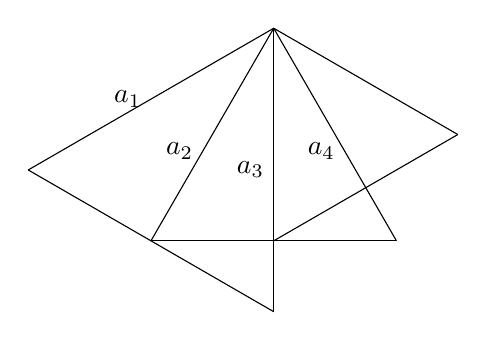
\begin{tikzpicture}[scale=1.8,]
    \foreach \x/\xlen in {-150/2, -120/1.732, -90/2, -60/1.732, -30/1.5}
    {
        \draw(0,0)--(\x:\xlen);
    }
\draw (-150:2)--(-90:2); 
\draw (-120:1.732)--(-60:1.732); 
\draw (-90:1.5)--(-30:1.5); 

\foreach \x in {1,2,3,4}
{
    \node at (-180+30*\x:1)[left]{$a_{\x}$};
}
\end{tikzpicture}
    \caption{}\label{fig:triangle}
\end{figure}


\begin{solution}
  如\cref{fig:triangle},设第 $k$ 个这样的正三角形的边长为 $a_k$,高为 $h_k$, 面积为 $A_k,\; (k=1,2,\ldots,10)$,于是
\[a_1=a,\qquad h_1=\frac{\sqrt{3}}{2}a,\qquad A_1=\frac{1}{2}a_1h_1=\frac{\sqrt{3}}{4}a^2\]
因为所有正三角形都相似,故对应边与对应高线成比例,即
\[\frac{a_{k+1}}{a_{k}}=\frac{h_{k+1}}{h_k}\]
又依三角形的作法,知
\[a_{k+1}=h_k,\qquad (k=1,2,3,\ldots,10)\]
\[\therefore\quad \frac{a_{k+1}}{a_{k}}=\frac{h_{k+1}}{a_{k+1}}=\frac{h_1}{a_1}=\frac{\sqrt{3}}{2}\]
根据相似三角形面积之比等于对应边平方之比,故
\[q=\frac{A_{k+1}}{A_k}=\frac{a^2_{k+1}}{a^2_k}=\left(\frac{a_{k+1}}{a_k}\right)^2=\left(\frac{\sqrt{3}}{2}\right)^2=\frac{3}{4}\]
因此,前 10 个正三角形面积之和
\[S_{10}=\frac{\dfrac{\sqrt{3}}{4}a^2\left[1-\left(\dfrac{3}{4}\right)^{10}\right]}{1-\dfrac{3}{4}}=\sqrt{3}a^2\left[1-\left(\frac{3}{4}\right)^{10}\right]\]
\end{solution}

{\linespread{1.65}\selectfont 为书写简便起见,我们用符号 $\sum\limits^n_{i=m}a_i$ 表示数列 $\{a_i\}$ 的相邻的一些项的和。整数 $i$ 在确定了的界限内变动,在 $\sum$ 的下面和上面的数字分别表示求和的起止项的序号,符号“$\sum$”读作 sigma。例如\par}
\[\begin{split}
    \sum^n_{i=1}a_i&=a_1+a_2+\cdots+a_n\\
    \sum^n_{i=k}a_i&=a_k+a_{k+1}+\cdots+a_n\\
\end{split}\]

在许多数学问题里,我们需要求出以下标 $i$ 的 $k$ 次多项式 $f(i)$ 为通项的前 $n$ 项和的公式:
\[S_k(n)=\sum^{n-1}_{i=0}f(i)=f(0)+f(1)+\cdots+f(n-1)\]
这里的指标集是非负整数集。

数列 $\{S_k(n)\}$ 称为数列 $\{f(n)\}$ 的和数列,即
\[\begin{split}
    S_k(1)&=f(0)\\
    S_k(2)&=f(0)+f(1)\\
    S_k(3)&=f(0)+f(1)+f(2)\\
    \cdots
\end{split}\]

为讨论方便起见,规定 $S_k(0)=0$, 于是和数列 $\{S_k(n)\}$ 满足下面两个性质:
\begin{enumerate}[itemindent=3.5em]
    \item $S_k(0)=0$
    \item $S_k(n+1)-S_k(n)=f(n),\qquad n=0,1,2,\ldots$
\end{enumerate}

我们来考虑这样一个多项式,它在 $k$ 个点 $0,1,2,\ldots,k-1$ 处与横坐标轴相交,又通过 $(k,1)$ 点,显然这个关于 $n$ 的多项式为
\[q_k(n)=\frac{n(n-1)\cdots(n-k+1)}{k!}\]
下面来求数列 $\{q_k(n)\},\; n=0,1,2,\ldots$ 的前 $n$ 项和的公式。

\begin{example}\label{exp:sum_of_qk}
设 $q_k(n)=\dfrac{1}{k!}n(n-1)\cdots(n-k+1)$,则前 $n$ 项的和
\[\begin{split}
    S_k(n)&=\sum^{n-1}_{i=0} q_k(i)=q_k(0)+q_k(1)+\cdots+q_k(n-1)\\
    &=\frac{1}{(k+1)!}n(n-1)\cdots(n-k)
\end{split}\]
换言之,其和是这样一个多项式,它在 $0,1,2,\ldots,(k-1)$,共 $k$ 个点处与坐标轴相交且通过 $((k+1),1)$ 点。
\end{example}

\begin{solution}
设 $S_k(n)$是一个 $n$ 的 $k+1$ 次多项式,且让 $S_k(n)$ 满
足条件:
\begin{align}
    \label{eq:Skn}S_k(0)&=0\\
    \label{eq:Skn+1}S_k(n+1)-S_k(n)&=q_k(n)
\end{align}
由于 $q_k(0)=q_k(1)=\cdots=q_k(k-1)=0$,且 $q_k(k)=1$,于是
\begin{equation}
    \begin{split}
 S_k(n)&=q_k(0)+q_k(1)+\cdots+q_k(n-1)\\
&=\underbrace{0+0+\cdots+0}_{\text{$k$项}}+1+(k+1)+\\
&\qquad \cdots+
\frac{1}{k!}(n-1)(n-2)\cdots(n-k)     
    \end{split}
\end{equation}

由\cref{eq:Skn,eq:Skn+1} 得到
\begin{align}
S_k(0)=S_k(1)=\cdots=S_k(k)=0\\
\label{eq:Skk+1}S_k(k+1)=1
\end{align}
从而知道 $S_k(n)$ 有下面 $k+1$ 个因式,即
\[S_k(n)=Cn(n-1)(n-2)\cdots(n-k)\]
这里 $C$ 是未定的常数因子。

常数因子 $C$ 可由\cref{eq:Skk+1} 确定,
\[S_k(k+1)=C(k+1)k(k-1)\cdots2\cdot 1=1\]
\[\therefore\quad C=\frac{1}{(k+1)!}\]

此处记 $(k+1)!=1\cdot 2\cdot 3\cdots k(k+1)$。

因此,
\[\begin{split}
    S_k(n)&=\sum^{n-1}_{i=0} q_k(i)=\sum^{n-1}_{i=0} \frac{1}{k!}i(i-1)\cdots (i-k+1)\\
    &=\frac{1}{(k+1)!}n(n-1)\cdots (n-k)
\end{split}\]
\end{solution}

我们也常用这样一种想法来求数列前 $n$ 项和的公式,即如果数列的通项能分解成另一个数列相邻两项的差:

$f(n)=F(n+1)-F(n),\; n=0,1,2,\ldots$时,那么前 $n$ 项的和
\[\begin{split}
   S(n)&= \sum^{n-1}_{i=0} f(i)= \sum^{n-1}_{i=0} [F(i+1)-F(i)]\\
   &=[F(1)-F(0)]+[F(2)-F(1)]+\cdots +[F(n)-F(n-1)]\\
   &=F(n)-F(0)
\end{split}\]


\begin{example}
    求 $S(n)=\dfrac{1}{1\cdot 4}+\dfrac{1}{4\cdot 7}+\dfrac{1}{7\cdot 10}+\cdots +\dfrac{1}{(3n-2)(3n+1)}$ 的和。
\end{example}

\begin{solution}
$\because\quad \dfrac{1}{(3i-2)(3i+1)}=\dfrac{1}{3}\left(\dfrac{1}{3i-2}-\dfrac{1}{3i+1}\right)$

\bigskip 当 $i=1,2,3,\ldots,n$ 时,有
\[\begin{split}
    \frac{1}{1\cdot 4}&=\frac{1}{3}\left(\frac{1}{1}-\frac{1}{4}\right)\\
    \frac{1}{4\cdot 7}&=\frac{1}{3}\left(\frac{1}{4}-\frac{1}{7}\right)\\
    \cdots &\cdots\\
    \frac{1}{(3n-2)(3n+1)}&=\frac{1}{3}\left(\frac{1}{3n-2}-\frac{1}{3n+1}\right)
\end{split}\]
因此:
\[\begin{split}
    S(n)&=\sum^n_{i=1}\frac{1}{(3i-2)(3i+1)}\\
    &=\frac{1}{3}\left(\frac{1}{1}-\frac{1}{3n+1}\right)\\
    &=\frac{n}{3n+1}
\end{split}\]
\end{solution}

如果数列的通项是以其它形式的 $k$ 次多项式给出的,我们可以用待定系数法把它变形为\cref{exp:sum_of_qk} 的形式。


\begin{example}
  求 $S_2(n+1)=0^2+1^2+2^2+\cdots+n^2$ 的和。
\end{example}

\begin{solution}
  设 $i^2=\lambda \dfrac{i(i-1)}{2!}+\mu i,\; (i=0,1,2,\ldots,n)$,由待定系数法求得:
\[\lambda=2,\qquad \mu=1\]
于是:
\[S_2(n+1)=\sum^n_{i=0}i^2=2\sum^n_{i=0}\frac{i(i-1)}{2!}+\sum^n_{i=0}i\]
应用\cref{exp:sum_of_qk} 的结果,得到:
\[\begin{split}
    S_2(n+1)&=2\frac{(n+1)n(n-1)}{3!}+\frac{n(n+1)}{2}\\
    &=\frac{n(n+1)(2n+1)}{6}
\end{split}\]
\end{solution}

\begin{example}
设 $a_0,a_1,a_2,\ldots,a_n$ 成等差数列,求 $S_n=a_0+a_1x+a_2x^2+a_3x^3+\cdots+a_nx^n$ 的和。    
\end{example}

\begin{solution}
  \begin{equation}
    \label{eq:sum_anxn}
    S_n=a_0+a_1x+a_2x^2+a_3x^3+\cdots+a_nx^n
  \end{equation}
由于\cref{eq:sum_anxn} 中的系数成等差数列,变量 $1,x,x^2,\ldots,x^n$ 成等比数列,利用等差数列的任意相邻的三项有递归关系:
\begin{equation}
    a_n-2a_{n-1}+a_{n-2}=0,\qquad n\geqslant 2
\end{equation}
知道\cref{eq:sum_anxn} 相邻的三项下面等式成立:
\begin{equation}
  \label{eq:zero_item}
  a_nx^n-2x(a_{n-1}x^{n-1})+x^2(a_{n-2}x^{n-2})=0,\qquad n\geqslant 2
\end{equation}
让\cref{eq:sum_anxn} 的两边分别乘以 $1,-2x,x^2$, 然后相加,得
\[\begin{split}
    S_n&=a_0+a_1x+a_2x^2+a_3x^3+\cdots+a_{n-1}x^{n-1}+a_nx^n\\
    -2xS_n&=-2a_0x-2a_1x^2-2a_2x^3-\cdots-2a_{n-1}x^n-2a_nx^{n+1}\\
    x^2S_n&=a_0x^2+a_1x^3+a_2x^4+\cdots+a_{n-1}x^{n+1}+a_nx^{n+2}
\end{split}\]
所以:
\[(1-x)^2 S_n=a_0+(a_1-2a_0)x+0+\cdots+0+(a_{n-1}-2a_n)x^{n+1}+a_nx^{n+2}\]
由\cref{eq:zero_item} 可知在上面等式中,其余各项为 0,若 $x\neq 1$,两边除以 $(1-x)^2$,得
\[S_n=\frac{a_0+(a_1-2a_0)x+0+\cdots+0+(a_{n-1}-2a_n)x^{n+1}+a_nx^{n+2}}{(1-x)^2}\]
若 $x=1$,原题就变成求等差数列前 $n$ 项的和,这时,
\[S_n=\frac{n(a_1+a_n)}{2}\]
\end{solution}

\begin{example}
    数列 $\{v_n\}$ 由下面递归定义给出:
 \[ v_{n+1}=3v_n-2v_{n-1},\quad v_0=2,\quad v_1=3,\; n=1,2,3,\ldots\]
 求:$v_n$,$S_n=\sum\limits^{n-1}_{i=0}v_i$。
\end{example}

\begin{solution}
    由 $v_{n+1}=3v_n-2v_{n-1}$ 容易看出
  \[  v_{n+1}-v_{n}=2(v_n-v_{n-1})\]
    设 $q_n=v_{n+1}-v_n$,$q_{n-1}=v_n-v_{n-1}$, 则 $q_n=2q_{n-1},\; (n=1,2,\ldots)$,换言之,$\{q_n\}$ 是公比为 2 的等比数列,
\[\therefore\quad q_n=2q_{n-1}=2^2q_{n-2}=\cdots=2^n(v_1-v_0)=2^n(3-2)=2^n\]
从而:
\[\begin{split}
    q_{n-1}&=v_n-v_{n-1}=2^{n-1}\\
v_n&=(v_n-v_{n-1})+(v_{n-1}-v_{n-2})+\cdots+(v_1-v_0)+v_0\\
&=2^{n-1}+2^{n-2}+\cdots +2+1+2\\
&=(2^n-1)+2=2^n+1\\
\end{split}\]
\[\begin{split}
    S_n=\sum^{n-1}_{i=0}v_i&=\sum^{n-1}_{i=0}(2^i+1)=\sum^{n-1}_{i=0}2^i+\sum^{n-1}_{i=0}1\\
    % &=\sum^{n-1}_{i=0}2^i+\sum^{n-1}_{i=0}1\\
    &=(2^n-1)+n=2^n+(n-1)
\end{split}\]
\end{solution}

\begin{Exercise}
\begin{question}
  \item 在等差数列中
  \begin{tasks}(2)
    \task 若 $a_5=100$, $d=\frac{1}{2}$,求$a_{100}$;
    \task 若 $a_3=-4$, $a_5=2$, 求 $a_{10}$;
    \task 若 $a_p=q$, $a_q=p$, 求 $a_{p+q}$;
    \task 用 $a_s$, $a_1$, $d$ 表示 $a_n$。
  \end{tasks}

\item 在 7 和 35 之间插入 6 个数使它们和已给两数组成等差数列。
\item 在 8 和 32 之间应插入多少个等差中项,可使等差中项中的前两个数的和与后两个数的和之比为 $7:25$。
\item 求证含有奇数个项的等差数列里,第一项,中间项,最后项也成等差数列。
\item 在三位数里有几个是 6 的倍数,求它们的和。
\item 求 $S_n=1-2+3-4+5-\cdots+(-1)^{n+1}n$ 的和。
\item 一等差数列前 $n$ 项之和为 $S_n=5n^2+3n$,求 $a_n$。
\item 在等差数列中
\begin{tasks}
  \task 已知 $d=2$, $n=15$, $a_{15}=-10$, 求 $S_{15}$;
  \task 已知 $a_n$, $S_n$ 和 $a_1$,求 $d$;
  \task 已知 $d$, $S_n$ 和 $a_1$,求 $n$;
  \task 已知 $a_n$, $S_n$ 和 $d$, 求 $a_1$。
\end{tasks}

\item 求等差数列 $2\dfrac{1}{2},1\dfrac{5}{6},1\dfrac{1}{6},\ldots$ 的第 $n$ 项,并求这个等差级数的最大和。

\bigskip
\item 在等差数列中,若 $S_1=a_1+a_3+\cdots+a_{2n-1}=44$,$S_2=a_2+a_4+\cdots+a_{2n-2}=33$,求 $a_n$。
\item 某化工厂为了加固烟囱,要在烟囱上打 32 道铁箍,且使每两道铁箍之间的距离相等,已知最上面一道铁箍处烟囱的外直径为 \qty{1.5}{m},最下面一道箍处烟囱的外直径为 \qty{3.5}{m}。求全部铁箍用料的总长。

\item 若 $a_1,a_2,\ldots,a_n$ 成等差数列,求证:
\[\frac{1}{\sqrt{a_1}+\sqrt{a_2}}+\frac{1}{\sqrt{a_2}+\sqrt{a_3}}+\cdots +\frac{1}{\sqrt{a_{n-1}}+\sqrt{a_n}}=\frac{n-1}{\sqrt{a_1}+\sqrt{a_n}}\]

\item 求下列各等比数列的通项公式
\begin{tasks}(2)
    \task $-1,\;-2,\;-4,\;\ldots$
    \task $-1,\;1,\;-1,\;\ldots$
    \task $\dfrac{2}{3},\;\dfrac{1}{2},\;\dfrac{3}{8},\;\ldots$
    \task $\sqrt{2},\;1,\;\dfrac{\sqrt{2}}{2},\;\ldots$
    \task $1,\;-\sqrt{\dfrac{1}{3}},\;\dfrac{1}{3},\;\ldots$
\end{tasks}

\item 在等比数列里
\begin{tasks}
  \task $a_1=36$, $a_5=2\dfrac{1}{4}$,求 $q$ 和 $S_5$;
  \task $a_n=1296$, $q=6$, $S_n=625$,求 $a_0$ 和 $a_1$;
  \task $a_1=3$, $q=\dfrac{1}{3}$, $n=8$,求 $S_8$;
  \task $S_5=242$, $q=3$,求 $a_5$。
\end{tasks}
\item 在等比数列里,若 $a_7-a_5=a_6+a_5=48$, 求 $a_1$, $q$ 和 $S_{10}$。
\item 在 160 和 5 之间插入 4 个数,使这 6 个数成等比数列,求这 4 个数。
\item 求证,若 $a_1,a_2,\ldots,a_n,\ldots\; (a_i>0,i=1,2,3,\ldots)$ 成等比数列,则以下数列均成等比数列:
\begin{tasks}(2)
  \task $a_1,\; a_3,\; \ldots, a_{2n-1},\; \ldots$;
  \task $ka_1,\; ka_3,\; \ldots, ka_{2n-1},\; \ldots$;
  \task $\dfrac{1}{a_1},\; \dfrac{1}{a_2},\; \ldots, \dfrac{1}{a_{n}},\; \ldots$;
  \task $a^2_1,\; a^2_2,\; \ldots, a^2_{n},\; \ldots$;
  \task $\sqrt{a_1},\; \sqrt{a_2},\; \ldots, \sqrt{a_n},\; \ldots$。
\end{tasks}

\item 从盛满 \qty{20}{L} 纯酒精的容器里倒出 \qty{1}{L},然后用水填满,再倒出 \qty{1}{L} 混合溶液,用水填满,这样继续进行,一共倒三次,这时容器里有纯酒精多少?
\item 甲厂产量是乙厂产量的 40.96\%,甲厂产品每年增长的百分率比乙厂产品每年增长的百分率多 30\%,若第四年甲厂产量和乙厂产量相同,求甲厂每年产品平均增长的百分率是多少?
\item 一个机器制造厂的原订的三年计划,每年比上一年增产的机器台数相同,但到了第三年,由于实际需要,须比原计划多生产 1000 台,那么每年比上一年的增长百分数就相同,而且第三年的台数恰为原计划总台数的一半,问实际上每年生产了多少台?每年比上一年增长的百分数是多少?
\item 某农机厂去年十月份生产拖拉机 1000 台,这样连同一月至九月的产量恰好完成全年生产任务,为加速农业机械化,全厂在年底前又生产了 2310 台,于是就超额完成全年计划的 21\%。求
\begin{tasks}
  \task 今年十一、十二月份每月平均增长率;
  \task 今年原计划生产量。
\end{tasks}

\item 若一个三角形的三个角成等差数列,而它的边成等比数列,求这个三角形的形状。
\item 已知一个正三角形边长为 $a$,以此正三角形的高线为边做第二个三角形,依此类推,求前 10 个正三角形的周长的和。
\item 求 $(x+y)+(x^2+xy+y^2)+(x^3+x^2y+xy^2+y^3)+\cdots$ 的前 $n$ 项的和。
\item 求 $7+77+777+\cdots$ 的前 $n$ 项的和。
\item 设等比数列 $a_1,a_2,\ldots,a_n,\ldots$ 的公比是 $q$。求证:$a_1a_2\cdots a_n=a^n_1q^{\tfrac{n(n-1)}{2}}$

\item 求下列各数列的和
\begin{tasks}(3)
    \task $\displaystyle \sum^{n-1}_{i=0} i^3$
    \task $\displaystyle \sum^{n-1}_{i=0} i^4$
    \task $\displaystyle \sum^{n-1}_{i=0} (i-1)i$
    \task $\displaystyle \sum^{n-1}_{i=0} (2i-1)^2$
    \task $\displaystyle \sum^{n-1}_{i=0} \frac{2i+1}{i^2\cdot (i+1)^2}$
\end{tasks}

\item 数列 $a_0,a_1,\ldots, a_n,\ldots$ 中的 $a_0,a_1$ 为已知,且 $a_n=\dfrac{a_{n-1}+a_{n-2}}{2},\; n=2,3,4,\ldots$,求 $a_n$。
\item 数列 $a_1,a_2,\ldots,a_n,\ldots$中,$a_1=2$,且$a_n=3a_{n-1}+1\; (n=2,3,4,\ldots )$, 求 $a_1+a_2+\cdots +a_n$。
\item 已知数列 $a_1,a_2,\ldots ,a_n,\ldots$ 的相邻两项 $a_n$,
$a_{n+1}$ 是方程 $x^2+3nx+c_n=0,\; (n=1,2,\ldots)$ 的两根,当 $a_1=1$ 时,求 $\sum\limits^{2p}_{n=1}c_n$。
\item $n$ 是非负的整数,试问同时满足下面三个不等式的整数对 $(x,y)$ 共有多少组?
\[y\geqslant x,\qquad y\leqslant 3x,\qquad y\leqslant n\]
\item 三角形三条边的长分别是$\ell$, $m$ 和 $n$,这里 $\ell$,$m$,
$n$都是正整数,且$\ell\leqslant m\leqslant n$,对于每一个给定的$n$(取
$n=1,2,3,\ldots$),所说的不同形状的三角形有多少个?求
出三角形的个数用 $n$ 表示的一般公式。
\item 数列 $\{a_n\}$ 是:
\[a_1=\frac{1}{3},\qquad \frac{1}{a_{n+1}}-\frac{1}{a_n}=2n+3\quad (n=1,2,3,4,\ldots)\]
\begin{tasks}
  \task 用 3 的式子表示一般项;
  \task 用 $n$ 的式子表示前 $n$ 项的和 $\displaystyle\sum^n_{k=1}a_k$
\end{tasks}

\item 若数列 $\{a_n\}$ 是等差数列,
求证:\[\frac{1}{a_1a_2}+\frac{1}{a_2a_3}+\cdots+\frac{1}{a_{n-1}a_n}=\frac{n-1}{a_1a_n}\]
\end{question}
\end{Exercise}

\section{数学归纳法}
现在我们研究在数学中常用的一种证明方法——数学归纳法。

我们常常从一些特殊事实归纳出一般结论,这种推理方法就是通常说的归纳法,用归纳法可以帮助我们从特殊情况发现一般规律,但如果归纳时所根据的特殊事实没有完全包括结论中所涉及到的所有情况,结论可能不正确,这就是说:命题可能对于一系列的特别情形是对的,但是一般并不正确。

例如,已知函数 $f(n)=(n^2-5n+5)^2$,则
\[f(1)=1,\qquad f(2)=1,\qquad f(3)=1,\qquad f(4)=1 \]
如果我们由此得出结论 $f(n)=(n^2-5n+5)^2=1$ ($n$ 是任何自然数),那就是错误的,事实上,$f(5)=25$,不等于1。

为了克服这种归纳法的不完全性,我们常采用下述的数学归纳法来证明一个关于自然数 $n$ 的命题。

数学归纳法的证明逻辑是:

对于一个依赖于自然数 $n=1,2,3,\ldots$ 的命题 $p(n)$,如果
\begin{enumerate}
  \item 当 $n=1$ 时,命题 $p(1)$ 正确;
  \item 假设 $n=k,\; (k\geqslant 1)$ 时,命题 $p(k)$ 正确,可以推出 $n=k+1$ 时,命题 $p(k+1)$ 正确,那么,命题 $p(n)$ 对于一切自然数 $n=1,2,3,\ldots$ 都正确。
\end{enumerate}

这个方法的根据,就是自然数的基本性质:

\begin{Theorem}[自然数的基本性质]{性质}
  令 $A$ 是自然数集 $\mathbb{N}$ 中具有下面性质的子集:
\begin{enumerate}
  \item\label{itm:prop1} $1\in A$;
  \item\label{itm:prop2} 若 $n\in A$,则 $n+1\in A$
\end{enumerate}
那么:$A=\mathbb{N}$。
\end{Theorem}

现在,我们来证明数学归纳法的正确性,设使命题 $p(n)$ 成立的自然数是自然数集 $\mathbb{N}$ 中的子集 $A$,即 $A\subseteq \mathbb{N}$。

根据数学归纳法中的 \ref{itm:prop1},$1\in A$; 再根据数学归纳法中的 \ref{itm:prop2},若 $n\in A$,则 $n+1\in A$。于是,根据自然数的基本性质,得到
\[A=\mathbb{N}\]
因此,命题 $p(n)$ 对于一切自然数成立。

下面举一些例子说明这个方法的应用。

\begin{example}
  求证:
  \begin{equation}
    \label{eq:sum_n}
    1+2+3+\cdots+n=\frac{n(n+1)}{2}
  \end{equation}
\end{example}

\begin{analyze}
    我们注意到和式:$1+2+3+\cdots+n$ 可以递归地定义为
\[\begin{cases}
    S(1)=1\\
    S(n)=S(n-1)+n,\qquad n=2,3,\ldots
\end{cases}\]
上面的等式为应用数学归纳法去证明打下了基础。
\end{analyze}

\begin{proof}
  \begin{enumerate}
    \item\label{itm:proof1} 当 $n=1$ 时,$\because\, S(1)=1,\quad \dfrac{1\times(1+1)}{2}=1$,$\therefore\, $ \cref{eq:sum_n} 成立。
    \item\label{itm:proof2} 假设 $n=k,\; (k\geqslant 1)$ 时,\cref{eq:sum_n} 成立,即有
\[S(k)=1+2+3+\cdots+k=\frac{k(k+1)}{2}\]
那么,当 $n=k+1$ 时,
\[S(k+1)=1+2+3+\cdots+k+(k+1)=S(k)+(k+1)\]
应用数学归纳法假设于上面的等式,得到
\[\begin{split}
    S(k+1)&=\frac{k(k+1)}{2}+(k+1)=(k+1)\left(\frac{k}{2}+1\right)\\
    &=\frac{(k+1)(k+2)}{2}\\
    &=\frac{(k+1)[(k+1)+1]}{2}
\end{split}\]
即\cref{eq:sum_n} 仍成立。

由所证 \ref{itm:proof1} 和 \ref{itm:proof2} 两步知:
\[1+2+3+\cdots+n=\frac{n(n+1)}{2}\]
对于一切自然数 $n$ 都成立。
\end{enumerate}
\end{proof}

从上例明显地看出,用数学归纳法证明一个命题的步骤是:
\begin{enumerate}
\item\label{itm:stp1} 验证命题 $p(n)$,当 $n$ 取第一个值 $n=1$ 时,$p(1)$ 正
确。这一条是数学归纳法的基础。
\item\label{itm:stp2} 假设当 $n=k,\; (k\geqslant 1)$时,命题 $p(k)$ 正确,证明当 $n=k+1$ 时,命题 $p(k+1)$ 也正确。这一条是说性质 $p(n)$ 具有遗传性,可以一代一代地传下去。完成了这两步以后,就可以断定命题 $p(n)$ 对于一切自然数 $n$ 都正确。因为首先证明 $p(1)$ 正确,另外由 $p(1)$ 正确推出 $p(2)$ 正确,由 $p(2)$ 正确推出了 $p(3)$ 正确,依次下去,便可知对于一切自然数 $n$,$p(n)$ 正确。
\end{enumerate}


有时不一定从 1 开始,也就是数学归纳法里两句话,可以改成
\begin{enumerate}
  \item 当 $n=k_0$ 时,命题 $p(k_0)$ 正确。
  \item 从假设 $n=k,\; (k\geqslant k_0)$ 时,这个命题 $p(k)$ 正确,可以推出当 $n=k+1$ 时,这个命题 $p(k+1)$ 也正确,那么 $p(n)$ 对于 $n\geqslant k_0$ 都正确。
\end{enumerate}

\begin{example}
  假设我们只有面额是 3 分和 5 分的两种邮票,试证明可以用面额是 3 分和 5 分的两种邮票去付多于 7 分的任意一
笔邮资。

如果我们对于每一种情形逐一地去证明,譬如,用 3 分和 5 分的邮票各一张可以付 8 分的邮资;用 3 分的邮票 3 张可以付 9 分的邮资,用 5 分的邮票 2 张可以付 10 分的邮资等等,照这样一个一个地验证下去,不是有成效的,因为有无数多种的情况需要去验证,让我们用数学归纳法来证明。
\end{example}

\begin{proof}
\begin{enumerate}
  \item\label{itm:exstep1} 我们对于 8 分的邮资,可以用 3 分和 5 分的邮票各一张去付,因此,当 $n=8$ 时,命题正确。
  \item\label{itm:exstep2} 假设用 3 分邮票和 5 分的邮票可以付 $k$ 分的邮资,我们要证明这两种邮票也可以用来付 $k+1$ 分的邮资。

  因为 $k\geqslant 8$,有两种可能的情形:$k$ 分的邮资至少要用一张 5 分的邮票去付;$k$ 分的邮资完全可以用 3 分的邮票去付。

  在第一种情形下,要付 $k+1$ 分的邮资,只要原来的某一张 5 分的邮票换以两张 3 分的邮票就可以了;

  在第二种情形下,3 分的邮票至少要有 3 张。要付 $k+1$ 分的邮资,只要把原来的三张 3 分邮票换以两张 5 分的邮票就可以了。

  根据 \ref{itm:exstep1} 和 \ref{itm:exstep2},可以断定 $n$ 为任何大于 7 的自然数,命题正确。
\end{enumerate}

\bigskip
数学归纳法这两步骤,是缺一不可的,从求函数 $f(n)=(n^2-5n+5)^2$ 的值可知,缺少了步骤 \ref{itm:stp2} 就得出不正确的结论,同样缺少了步骤1也可能得出不正确的结论。例如,由于没有验证数学归纳法中的第一条,而得出下面荒谬的结论:
\[2+4+6+\cdots+2n=n^2+n+1\]

我们在下面只证明数学归纳法中的 \ref{itm:stp2}。

假设 $n=k,\; (k>1)$,等式 $2+4+6+\cdots+2k=k^2+k+1$ 成立,那么,当 $n=k+1$ 时,
\begin{align*}
    2+4+6+\cdots+2k+2(k+1)&=(2+4+6+\cdots+2k)+2(k+1)\\
&=k^2+k+1+2(k+1)  \tag{数学归纳法假设}\\
&=(k+1)^2+(k+1)+1
\end{align*}
由此知,当 $n=k+1$ 时,等式仍成立。如果仅从数学归纳法中的 \ref{itm:stp2} 就得出等式对于任何自然数都成立,那是错误的。

事实上,当 $n=1$ 时,等式左边 $=2$,右边 $=1^2+1+1=3$,因此,上面的等式是错误的。
\end{proof}

\begin{example}
    证明:
\[S(n)=1-2^2+3^2-4^2+\cdots+(-1)^{n-1}n^2=(-1)^{n-1}\frac{n(n+1)}{2}\]
\end{example}

\begin{proof}
\begin{enumerate}
    \item 当$n=1$时,$S(1)=1$,又$(-1)^0\frac{1(1+1)}{2}=1$,所以等式成立。

\item 假设$n=k$时,有
\[S(k)=1-2^2+3^2-4^2+\cdots+(-1)^{k-1}k^2=(-1)^{k-1}\frac{k(k+1)}{2}\]
那么,当$n=k+1$时,有    
\[\begin{split}
    S(k+1)=S(k)+(-1)^k(k+1)^2&=(-1)^{k-1}\frac{k(k+1)}{2}+(-1)^k(k+1)^2\\
    &=(-1)^k(k+1)\left[-\frac{k}{2}+(k+1)\right]\\
    &=(-1)^k \frac{(k+1)(k+2)}{2}\\
    &=(-1)^k \frac{(k+1)[(k+1)+1]}{2}
\end{split}\]
\end{enumerate}

由1和2知,等式对于一切自然数 $n$ 都成立。
\end{proof}


\begin{example}
证明:
\[\begin{split}
    S(n)&= \sin \alpha+\sin (\alpha+\beta)+\sin (\alpha+2 \beta)+\cdots+\sin (a+(n-1) \beta) \\
&= \dfrac{\sin(n\beta/2)}{\sin(\beta/2)} \sin \left(\alpha+\dfrac{n-1}{2} \beta\right)
\end{split}\]
\end{example}

\begin{proof}
\begin{enumerate}
    \item\label{itm:proof1_triangle} 当 $n=1$ 时,
\[\because\, \text{左边}=S(1)=\sin\alpha,\quad \text{右边}=\dfrac{\sin(\beta/2)}{\sin(\beta/2)}\sin(\alpha+0\cdot \beta)=\sin\alpha, \quad\therefore\, \text{等式成立。}\]
% $\therefore\quad $ 等式成立。

\item\label{itm:proof2_triangle} 假设 $n=k$ 时,
\[\begin{split}
    S(k)&=\sin \alpha+\sin (\alpha+\beta)+\sin (\alpha+2 \beta)+\cdots+\sin (\alpha+(k-1) \beta) \\
&=\dfrac{\sin(k\beta/2)}{\sin(\beta/2)} \sin \left(a+\dfrac{k-1}{2} \beta\right)
\end{split}\]
成立,那么:
\[\begin{split}
    S(k+1)&= S(k)+\sin(\alpha+k\beta)\\
    &=\dfrac{\sin(k \beta/2)}{\sin(\beta/2)} \sin \left(a+\dfrac{k-1}{2} \beta\right)+\sin(\alpha+k\beta)\\
    &=\frac{1}{\sin(\beta/2)}\left[\sin\left(\alpha+\frac{k-1}{2}\beta\right)\sin\frac{k\beta}{2}+\sin(\alpha+k\beta)\sin\frac{\beta}{2}\right]\\
    &=\frac{1}{2\sin(\beta/2)}\left[\cos\left(\alpha-\frac{\beta}{2}\right)-\cos\left(\alpha+k\beta-\frac{\beta}{2}\right)\right. \\
    &\qquad \qquad \left. +\cos\left(\alpha+k\beta -\frac{\beta}{2}\right)-\cos\left(\alpha+k\beta+\frac{\beta}{2}\right)\right]\\
    &=\frac{1}{2\sin(\beta/2)}\left[\cos\left(\alpha-\frac{\beta}{2}\right)-\cos\left(\alpha+k\beta+\frac{\beta}{2}\right)\right]\\
    &= \frac{(-2)}{2\sin(\beta/2)}\sin\left(\frac{2\alpha+k\beta}{2}\right)\sin\left(\frac{-k\beta-\beta}{2}\right)\\
    &=\frac{1}{\sin(\beta/2)}\cdot \sin\left(\alpha+\frac{k}{2}\beta\right)\cdot \sin\frac{(k+1)\beta}{2}\\
    &=\frac{\sin[(k+1)\beta/2]}{\sin(\beta/2)}\sin\left[\alpha+\frac{(k+1)-1}{2}\beta\right]
\end{split}\]
即当 $n=k+1$ 时,等式仍成立。由 \ref{itm:proof1_triangle} 和 \ref{itm:proof2_triangle} 可知,等式对任何自然数 $n$ 都成立。
\end{enumerate}
\end{proof}

\begin{example}
  用数学归纳法证明,如果 $n$ 是一个正整数,那么 $x^{2n}-y^{2n}$ 能被 $x+y$ 整除。
\end{example}

\begin{proof}
\begin{enumerate}
    \item\label{itm:proof1_devision} 当 $n=1$ 时,$x^2-y^2=(x+y)(x-y)$ 能被
    $x+y$整除。
    \item\label{itm:proof2_devision} 假设当 $n=k$,($k$ 是自然数),$x^{2k}-y^{2k}$ 能被 $x+y$ 整除,那么当 $n=k+1$ 时,
\[\begin{split}
    x^{2(k+1)}-y^{2(k+1)}
    &=x^2\cdot x^{2k}-y^2\cdot y^{2k}\\
    &=x^2\cdot x^{2k}-x^2y^{2k}+x^2y^{2k}-y^2\cdot y^{2k}\\
    &=x^2(x^{2k}-y^{2k})+(x^2-y^2)\cdot y^{2k}
\end{split}\]
    
    因为 $x^{2k}-y^{2k}$ 与 $x^2-y^2$ 都能被 $x+y$ 整除,所以 $x^2(x^{2k}-y^{2k})+(x^2-y^2)y^{2k}$ 也能被 $x+y$ 整除,这就是说,$x^{2k+1}-y^{2k+1} $能
    被$x+y$整除。
\end{enumerate}  

根据 \ref{itm:proof1_devision} 和 \ref{itm:proof2_devision},命题成立。
\end{proof}

\begin{example}\label{exp:lines}
    平面上有 $n$ 条直线,其中任何两条不平行,任何
三条不过同一点,证明这 $n$ 条直线把平面分成 $f(n)=\dfrac{1}{2}
(n^2+n+2)$ 个部分。
\end{example}

\begin{proof}
\begin{enumerate}
    \item\label{itm:proof1_lines} 当 $n=1$ 时,直线把平面分成两部分(为了简单起见,也说分成两块),又
  \[f(1)=\frac{1}{2}(1^2+1+2)=2\]
    因此,$n=1$ 时命题成立。
   \item\label{itm:proof2_lines} 假设 $n=k$ 时命题成立,就是
\[f(k)=\frac{1}{2}(k^2+k+2)\]

我们要设法找出 $f(k+1)$ 与 $f(k)$ 的递归关系,即由$f(k)$ 求得 $f(k+1)$ 的关系。为此,我们在平面上再增加一条直线 $\ell$(\cref{fig:lines}),
\begin{figure}
  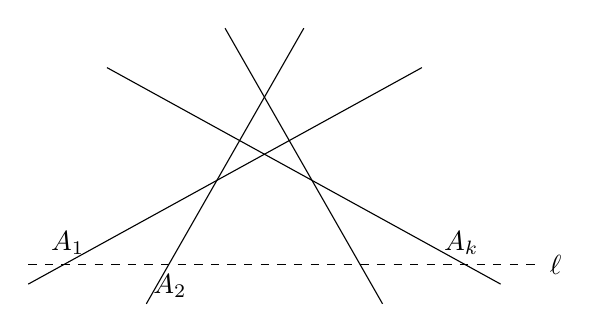
\begin{tikzpicture}%[very thick]
    \draw (1.5,-1)--(-.5,2.5);
    \draw (-1.5,-1)--(.5,2.5);
    \draw (-3,-.75)--(2,2);
    \draw (3,-.75)--(-2,2);
    \node at (-2.5,-.5) [above] {$A_1$};
    \node at (-1.2,-.5) [below] {$A_2$};
    \node at (2.5,-.5) [above] {$A_k$};
    \draw[dashed] (-3,-.5)--(3.5,-.5)node[right]{$\ell $};
  \end{tikzpicture}
  \caption{}\label{fig:lines}
\end{figure}
因为已知任何两条直线不平行,所以直线 $\ell$ 与平面上的原 $k$ 条直线都相交,而且这 $k$ 个交点互不相同,否则与任何三条直线不过同一点的已知条件矛盾,这 $k$ 个交点将直线 $\ell$ 分成 $k+1$ 段,因此直线 $\ell$ 越过原来的 $k+1$ 块平面部分,直线上的每段将它所在的原平面块分成两块,因此要给原来的平面部分的总数 $f(k)$ 增加 $k+1$ 块新的平面部分,就是
\[f(k+1)=f(k)+(k+1)\]
将 $f(k)=\dfrac{1}{2}(k^2+k+2)$ 代入上式,得到
\[\begin{split}
    f(k+1)&=\frac{1}{2}(k^2+k+2)+(k+1)\\
    &=\frac{1}{2}(k^2+3k+4)\\
    &=\frac{1}{2}[(k+1)^2+(k+1)+2]
\end{split}\]
这就是说,当 $n=k+1$ 时,命题也成立。



根据 \ref{itm:proof1_lines} 和 \ref{itm:proof2_lines},可知命题成立。
\end{enumerate}
\end{proof}

同学也许会问:\cref{exp:lines} 的结果是怎样发现的?数学归纳法能解决这个问题吗?其实此题的证明已经解决了这个问题,因为我们证明了 $f(n)$ 可以递归地定义为
\[\begin{cases}
    f(1)=2\\
    f(k+1)=f(k)+(k+1),\qquad k=1,2,\ldots,(n-1)
\end{cases}\]

首先 $f(1)$ 有定义,其次如果知道了 $f(1)$,就知道 $f(2)$,依次推下去,就知道$f(n)$。所以
\[\begin{split}
  f(n)&=[f(n)-f(n-1)]+[f(n-1)-f(n-2)]+\cdots +[f(2)-f(1)]+f(1)\\
  &=n+(n-1)+\cdots +2+2\\
  &=[n+(n-1)+(n-2)+\cdots +2+1]+1\\
  &=\frac{n(n+1)}{2}+1=\frac{n^2+n+2}{2}  
\end{split}\]


\begin{Exercise}
\begin{question}
    \item 用数学归纳法证明下列各等式: 
\begin{tasks}(2)
    \task $\displaystyle\sum^n_{k=1}3^{k-1}=\frac{3^n-1}{2}$
    \task $\displaystyle\sum^n_{k=1}k(k+1)=\frac{1}{3}n(n+1)(n+2)$
    \task $\displaystyle\sum^n_{k=1}\frac{1}{k(k+1)}=\frac{n}{n+1}$
    \task! \[\sum_{i=1}^{n}\cos[\alpha+(i-1)\beta]=\frac{\sin\dfrac{n\beta}{2}}{\sin\dfrac{\beta}{2}}\cos\left(\alpha+\frac{n-1}{2}\beta\right)\]
\end{tasks}

\item 用数学归纳法证明:
\begin{tasks}
\task 当 $n$ 是正整数时,$x^n-y^n$ 能被 $x-y$ 整除。
\task 当 $n$ 是正奇数时,$x^n+y^n$ 能被 $x+y$ 整除。
\task $(3n+1)7^n-1$ 能被 9 整除。
\task 邻近的三个自然数的立方和,必定能被 9 整除。
\task 当 $n$ 是正整数时,$(11)^{n+2}+(12)^{2n+1}$ 能被 133 整除。
\task 当 $n$ 是正整数时,$3^{2n+2}-8n-9$ 能被 64 整除。
\end{tasks}

\item 数列 $\{a_n\}$ 是这样确定的:
\[a1=1,\quad 4a_ka_{k+1}=(a_k+a_{k+1}-1)^2,\quad a_k<a_{k+1}\quad (k=1,2,3,\ldots)\]
\begin{tasks}
  \task\label{tsk:equation} 求 $a_2,a_3,a_4$, 并由此推断 $a_n$;
  \task 用数学归纳法证明 \ref{tsk:equation} 中推断出的 $a_n$ 的正确性。
\end{tasks}

\item 空间有$n$个平面,其中没有两个平面平行,没有三个平面相交于同一条直线,也没有四个平面过同一个点。求证:它们把空间分成 $f(n)=\frac{1}{6}(n^3+5n+6)$ 份。
\item 有 $n$ 个圆,其中每两个圆都相交于两点,并且每三个圆不相交于同一点。求证:这 $n$ 个圆把平面分成 $n^2-n+2$ 部分。
\item 若数列 $\{a_n\}$,当 $n\geqslant 3$ 时,满足条件
\[\frac{1}{a_1a_2}+\frac{1}{a_2a_3}+\frac{1}{a_3a_4}+\cdots+\frac{1}{a_{n-1}a_n}=\frac{n-1}{a_1a_n}\]
用数学归纳法证明数列 $\{a_n\}$ 是等差数列。
\end{question}
\end{Exercise}
\chapter{实数}\label{chp:real}
实数是现实世界中最基本的数系,我们采用逼近法来研究实数,逼近法是一种原理简朴但是应用广泛的方法,它将贯穿于本书的微积分学部分,是一支主力军。

\section{度量与实数}

一般说来,常见的量可以归纳成两类:比如一堆蛋,一群牛,它们都具有天然的个别单元,对它们的处理方法是数一数它们的个数,用来数个数的数学体系就是“自然数系”。另一类量如长度、重量、温度、压力这种量不具有天然不可分割的单元!我们处理这类量的办法是度量,由度量产生的数系就是“实数系”,换句话说,实数系乃是将常见的长度、重量等这一类量的通性加以抽象化、组织化所得出来的数学体系,它是用来表达、计算这一类连续变化的量的简洁、有效工具。

下面将以长度为例,说明度量和实数的起源。

\subsection{长度的度量}
因为长度这种量并不是有天然不可分割的单位,所以我们只好选用人为的单位长,设线段 $u$ 是所选用的单位长,当我们要度量一个线段 $a$ 时,我们所要去求的乃是 $a$ 与 $u$ 之间的“比值”,这个比值是一个实数 $k$, 我们就说线段 $a$ 的长度是 $k$ 单位,现在让我们耐心地分析一下,在实践中这个“比值”是怎样求得的?

我们先拿一根尺 $u$, 用它去逐段比量线段 $a$, 假如 $a$ 恰好是 $n$ 个和 $u$ 等长的线段首尾连接而成,我们说 $u$ 恰好整量 $a$, $a$ 的长度是 $n$ 单位,但是假如 $u$  不能整量 $a$,例如在\cref{fig:segments} 中的线段,$a$ 比 $4u$ 要长些,却比 $5u$ 要短些。

\begin{figure}
\begin{tikzpicture}
\draw (0,1)--node[above]{$u$}(1,1);
\foreach \x in {0,1}
{
    \draw (\x,1)--(\x,1.1);
}
\draw (0,0)--node[above=5pt]{$a$}(4.75,0);
\foreach \x in {0,1,...,4,4.25,4.5,4.75}
{
    \draw (\x,0)--(\x,0.1);
}
\end{tikzpicture}
    \caption{}\label{fig:segments}
\end{figure}

{
\linespread{1.6}\selectfont
试着去解决上述不能整量的矛盾的一个简朴想法是:把单位长 $u$ 适当地加以等分,希望分后的“分单位”能够整量 $a$(比如上面的例子中,$\dfrac{1}{4}u$ 就可以整量 $a$, 即 $a=4\dfrac{3}{4}u=\dfrac{19}{4}u$),一般地,假如 $a$ 能用 $\dfrac{1}{m}u$ 这个分单位整量,譬如 $a=\dfrac{n}{m}u$,则 $a,u$ 之间的比值是个有理数(也称为比数)。在这儿,就自然地产生下述基本问题。\par}

\bigskip
\emph{度量基本问题 } 任给两个量 $a,b$ 之间的比值是否一定是个有理数(比数)?换句话说,对于任给两个量 $a,b$ 是否存在一个同时整量 $a,b$ 的 $u$?

上面这个问题的重要性可以分别从正、反两面来分析:假如任何两个量的比值总是有理数,那么有理数全体就足够处理度量问题,这样度量问题就变得十分简单了。从另一方面来看,假如两个量之间的比值不一定是有理数,则有理数全体(简称有理数系或比数系)就不足以处理度量问题,换句话说,我们就得学会一个不只包含有理数系的实数系,才能充分处理度量问题。总之,上述基本问题是必须实事求是地弄明白的!

\subsection{无理数(非比实数)的存在}
不难给出,两个线段的比值不可能是有理数的一个简单例子,如\cref{fig:irrationalnumber} 所示,各边为单位长度的正方形的对角线 $\ell$ 与边长之比就不能是个有理数。
\begin{figure}
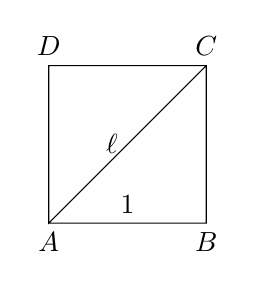
\begin{tikzpicture}
\draw (0,0)node[below]{$A$} --node[above]{1}(2,0)node[below]{$B$}-- (2,2)node[above]{$C$}--(0,2)node[above]{$D$}--(0,0)--node[left]{$\ell$}(2,2);
\end{tikzpicture}
\caption{}\label{fig:irrationalnumber}
\end{figure}

因为根据勾股定理,$\ell^2=2$, 所以,如果 $\ell$ 是个有理数,设其等于 $\dfrac{p}{q}$,这里 $q$ 和 $p$ 是两个互质的正整数,我们将有
\[p^2=2q^2\]
根据上述方程,$p$ 是偶数,因此 $p$ 本身也必定是偶数,譬如说,$p=2p'$, 用 $2p'$ 代替 $p$, 我们得到
\[4({p'}^2)=2q^2\]
或者,
\[q^2=2(p')^2\]
{\linespread{1.6}\selectfont
因而 $q^2$ 是偶数,于是 $q$ 也是偶数,然而这同我们所作的 $p$ 和 $q$ 没有公因子的约定相矛盾,这一矛盾是由假设对角线长能够表示为既约分数 $\dfrac{p}{q}$ 引起的,所以这一假设是错误的。\par}

这一用反证法推导的例子,表明符号 $\sqrt{2}$ 不能对应于任何有理数。另一例子是$\uppi$ ——圆的周长与直径的比,证明 $\uppi$ 不是有理数要复杂得多,并且直到近代才做到。不属于有理数系的实数有很多,所以在某种意义上远比有理数更为普遍,因此,从几何度量的客观实际需要出发,我们不得不增添一类新数,这一类新数叫\emph{无理数}。有理数和无理数的全体统称为\emph{实数系}。当我们面对着实数系中还存在着许多“无理数”这一事实时,怎样去有系统地学习实数系的性质并充分掌握其用法,这便成为我们的一个迫切的基本课题。下面所要谈的逼近法,就是一种有效地利用熟知的有理数系作为桥梁,向实数系进军的捷径。

\subsection{逼近法}
通过已知的有理数系去了解实数系的可能性基于下述基本事实,那就是:任何无理数都可以用有理数去逼近它!现在我们用数轴来图解有理数系与实数系间的关系。如\cref{fig:approximation} 所示。

\begin{figure}
\begin{tikzpicture}[>=latex, scale=1.3]
\draw[very thick, ->] (-0.8,0)--(8,0)node[right]{$\ell$};
\foreach \x/\xtext in {0/0,1/\dfrac{1}{q},2/\dfrac{2}{q},5.5/\dfrac{p}{q},6.5/\dfrac{p+1}{q}}
{
    \draw (\x, 0)node[below]{$\xtext$}--(\x,.1);
} 
\draw (5.9,0)--(5.9,.1)node[above]{$x$};
\end{tikzpicture}
    \caption{}\label{fig:approximation}
\end{figure}

{\linespread{1.6}\selectfont
在上面坐标系中,所有以整数为坐标的点,在直线 $\ell$ 上成一均匀分布的点集,其相邻两点间的距离都是 1 单位;同样的,所有坐标是 $\dfrac{p}{2}$, $(p=0,\pm1,\pm2,\ldots)$ 的点,在直线上成一均匀分布的点集,其相邻两点间的距离都是 $\dfrac{1}{2}$ 单位;设$q$为一指定的自然数,则所有坐标是 $\dfrac{p}{q},\; p\in\mathbb{Z}$ 的点在直线上成一均匀分布的点集,其相邻两点间的距离是 $\dfrac{1}{q}$ 单位。只要将 $q$ 取成足够大的自然数,则能使数 $\dfrac{1}{q}$ 想要多么小就可以多么小。这个现象说明在直线上任何一段很短的线段中,都有坐标是有理数的点,也就是任何两个有理数点之间都有有理数点,这就是\emph{有理数点集稠密性},但是这个现象并不表示有理点就可以填满整个直线,例如长度为 $\sqrt{2}$, $\sqrt{3}$ 的线段,若将它的一个端点放在数轴的原点,则另一端点在直线的坐标就不是有理数。现在我们的问题是如何说明实数同原来熟悉的有理数,因而最终同整数的关系。让我们再回到\cref{fig:approximation} 的数轴 $\ell$上,显然 $\ell$ 上面的每一个点或者是坐标为 $\dfrac{p}{q}$ 的有理点,或者处于两个相邻的有理点 $\dfrac{p}{q}$和$\dfrac{p+1}{q}$ 之间,换言之,给了任何自然数 $q$ 之后,对于每一个实数 $x$, 一定有一整数  $p$, 使得\par}
\[\frac{p}{q}\leqslant x<\frac{p+1}{q}\]
即
\[\frac{p}{q}\leqslant x<\frac{p}{q}+\frac{1}{q}\]
从这三个数各减去 $\dfrac{p}{q}$,得到
\[0\leqslant x-\frac{p}{q}<\frac{1}{q}\]
于是
\[\left|x-\frac{p}{q}\right|<\frac{1}{q}\]
这个不等式说明,只要将 $q$ 取成足够大的自然数,每一个实数 $x$ 与有理数 $\dfrac{p}{q}$ 的误差想要多么小就可以多么小。

下面我们来说明每一个无理数如何通过越来越逼近它的有理数数列来描述它。

\subsubsection{二分逼近法}

现在让我们用二分逼近法来说明任何无理数都可以用有理数数列去逼近它,使得误差小到任意小。

设某无理数 $x$ 位于线段 $A_0B_0=[a_0,b_0]$ 内(亦即$a_0<x<b_0$,$a_0$,$b_0$ 均为有理数),见\cref{fig:rationalnumber}。

\begin{figure}
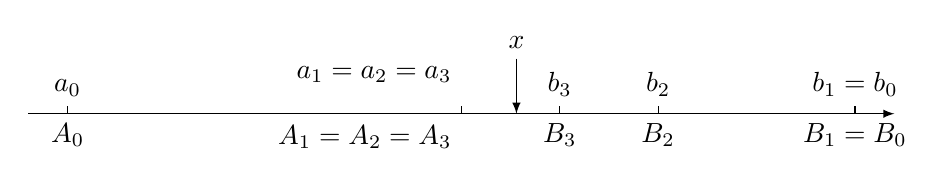
\begin{tikzpicture}[>=latex]
\draw[->] (-0.5,0)--(10.5,0);
\foreach \x/\xtext in {0/a_0,10/b_1=b_0,7.5/b_2,6.25/b_3}
{
    \draw (\x,0)--(\x,.1)node[above]{$\xtext$};
}  
\draw (5,0)--(5,.1);

\node at  (5,-.3)[left]{$A_1=A_2=A_3$};
\node at (6.25,0)[below]{$B_3$};
\node at (7.5,0)[below]{$B_2$};
\node at (0,0)[below]{$A_0$};
\node at (10,0)[below]{$B_1=B_0$};
\node at  (5,.5)[left]{$a_1=a_2=a_3$};
\draw[->] (5.7,.7)node[above]{$x$}--(5.7,0);
\end{tikzpicture}   
    \caption{}\label{fig:rationalnumber}
\end{figure}

{\linespread{1.6}\selectfont 我们将线段 $A_0B_0=[a_0,b_0]$ 等分为两段,亦即 $\left[a_0,\dfrac{a_0+b_0}{2}\right]$ 和 $\left[\dfrac{a_0+b_0}{2},b_0\right]$;而把 $x$ 所在的那一段叫做 $A_1B_1=[a_1,b_1]$,换句话说,当 $a_0<x<\dfrac{a_0+b_0}{2}$ 时,$a_1=a_0$,$b_1=\frac{a_0+b_0}{2}$;当 $\dfrac{a_0+b_0}{2}<x<b_0$,$a_1=\dfrac{a_0+b_0}{2}$,$b_1=b_0$。这样逐次二等分,由 $A_1B_1$ 求得 $A_2B_2$,\ldots,由 $A_{n-1}B_{n-1}$ 求得 $A_nB_n$,永远无休止地二等分下去,因为每次二等分后,分段长度减半,所以 $x$ 所在的线段就可以小到任何需要的程度。现在把上面的二分逼近过程写下来,就得到 $a_n,b_n,x$ 的下列关系:\par}
\begin{enumerate}
    \item $A_0B_0=[a_0, b_0]\supseteq A_1B_1 =[a_1,b_1]
    \supseteq \cdots \supseteq A_nB_n=[a_n, b_n]\supseteq A_{n+1}B_{n+1}=[a_{n+1},b_{n+1}]\supseteq \cdots \supseteq \{x\}$,即:
\[a_0\leqslant a_1\leqslant a_2\le\cdots\leqslant a_n\leqslant \cdots <x<\cdots\leqslant b_n\le\cdots\leqslant b_2\leqslant b_1\leqslant b_0\]

\item {\linespread{1.6}\selectfont $b_n-a_n=\dfrac{1}{2}(b_{n-1}-a_{n-1})=\cdots=\dfrac{1}{2^n}(b_0-a_0)$,这就保证了 $a_n$ 或 $b_n$ 和 $x$ 之间的误差小于 $\dfrac{1}{2^n}(b_0-a_0)$, 即 $|x-a_n|<\dfrac{1}{2^n}(b_0-a_0)$ 或 $|x-b_n|<\dfrac{1}{2^n}(b_0-a_0)$, 只要 $n$ 够大,上述误差就可以小到任意小。\par}
\item 实数 $x$ 由它的夹逼数列:
\[a_0\leqslant a_1\leqslant a_2\le\cdots\leqslant a_n\leqslant \cdots <x<\cdots\leqslant b_n\le\cdots\leqslant b_2\leqslant b_1\leqslant b_0\]
其中:$b_n-a_n=\dfrac{1}{2^n}(b_0-a_0)$ 唯一确定,即没有另一点能够处在所有的线段 $A_nB_n$ 之中。
\end{enumerate}

要证明这个数的唯一性,我们假定另有第二个数 $y$ 也属于一切线段 $A_nB_n$ 之中,于是这些线段的每一个长 $b_n-a_n$ 都应不小于 $|x-y|$, 但是,因为线段 $A_nB_n$ 可以任意小,只要 $n$ 足够大,$A_nB_n$ 的长就会小于 $x$ 和 $y$ 之间的距离,这就得出矛盾。所以实数 $x$ 能由它的夹逼数列唯一确定。

现在以 $x=\sqrt{2}$, $a_0=1$, $b_0=2$ 为例来说明如何用二分逼近法求 $\sqrt{2}$ 的近似值,如\cref{fig:sqrt2} 所示。
\begin{figure}
\begin{tikzpicture}[>=latex]
    \draw[->] (-0.5,0)--(10.5,0);
\foreach \x /\xtext in {0/a_0=a_1=1,10/b_0=2,5/{},2.5/a_2,3.75/a_3=a_4, 4.375/{}}
{
    \draw(\x,0)--(\x,.1)node[above]{$\xtext$};
}

\draw[->] (4.14,-.7)node[below]{$\sqrt{2}$}--(4.14,0);

\node at (5,-0.3)[right]{$b_1=b_2=b_3$};
\node at (4.375,-0.3){$b_4$};
\end{tikzpicture}
    \caption{}\label{fig:sqrt2}
\end{figure}

\begin{enumerate}
    \item  $\dfrac{1}{2}\left(a_{0}+b_{0}\right)=\dfrac{3}{2},\qquad \left(-\dfrac{3}{2}\right)^{2}=\dfrac{9}{4}>2 \quad\Rightarrow\quad\dfrac{3}{2}>\sqrt{2}$,
    
    故 $a_{0}=a_{1}=1,\qquad   b_{1}=\dfrac{3}{2}$

    \item   $\dfrac{1}{2}\left(a_{1}+b_{1}\right)=\dfrac{5}{4},\qquad \left(\dfrac{5}{4}\right)^{2}=\dfrac{25}{16}<2 \quad\Rightarrow\quad \dfrac{5}{4}<\sqrt{2}$
    
    故 $a_{2}=\dfrac{5}{4}, \qquad  b_{2}=b_{1}=\dfrac{3}{2}$

    \item  $\dfrac{1}{2}\left(a_{2}+b_{2}\right)=\dfrac{11}{8},\qquad \left(\dfrac{11}{8}\right)^{2}=\dfrac{121}{64}<2 \quad\Rightarrow\quad \dfrac{11}{8}<\sqrt{2}$
    
    故 $a_{3}=\dfrac{11}{8},\qquad  b_{3}=b_{2}=\dfrac{3}{2}$

    \item   $\dfrac{1}{2}\left(a_{3}+b_{3}\right)=\dfrac{23}{16},\qquad \left(\dfrac{23}{16}\right)^{2}=\dfrac{529}{256}>2 \quad\Rightarrow\quad \dfrac{23}{16}>\sqrt{2}$
    
    故 $a_{4}=a_{3}=\dfrac{11}{8},\qquad  b_{4}=\dfrac{23}{16}$

    \item  $\dfrac{1}{2}\left(a_{4}+b_{4}\right)=\dfrac{45}{32},\quad \left(\dfrac{45}{32}\right)^{2}=\dfrac{2025}{1024}<2 \quad\Rightarrow\quad \dfrac{45}{32}<\sqrt{2}$
    
     故 $a_{5}=\dfrac{45}{32}, \qquad b_{5}=b_{4}=\dfrac{23}{16}
    $
    
    \item  $\dfrac{1}{2}\left(a_{5}+b_{5}\right)=\dfrac{91}{64},\quad \left(\dfrac{91}{64}\right)^{2}=\dfrac{8281}{4096}>2 \quad\Rightarrow\quad \dfrac{91}{64}>\sqrt{2}$
    
     故 $a_{6}=a_{5}=\dfrac{45}{32}, \qquad b_{6}=\dfrac{91}{64}$

    
    \item  $\dfrac{1}{2}\left(a_{6}+b_{6}\right)=\dfrac{181}{128},\quad \left(\dfrac{181}{128}\right)^{2}=\dfrac{32761}{16314}<2 \quad\Rightarrow\quad \dfrac{181}{128}<\sqrt{2}$
    
    {\linespread{1.9}\selectfont 故 $a_{7}=\dfrac{181}{128}, \qquad b_{7}=b_{6}=\dfrac{91}{64}$,这时,$\dfrac{181}{128}<\sqrt{2}<\dfrac{91}{64}$,把 $\dfrac{181}{128}$ 作为 $\sqrt{2}$ 的不足近似值,其误差小于 $\dfrac{1}{2^7}=\dfrac{1}{128}$。\par}
\end{enumerate}

\medskip
{\linespread{1.6}\selectfont 照这样逐步计算,每次只要检验 $\dfrac{1}{2}(a_{n-1}+b_{n-1})$ 的平方和 2 之间的大小次序关系,就能确定 $\dfrac{1}{2}(a_{n-1}+b_{n-1})$ 应该是 $a_n$ 还是 $b_n$, 显然的,这样所求得的 $a_n,b_n$ 和 $\sqrt{2}$ 有下列关系:\par}
\[a_n<\sqrt{2}<b_n,\quad b_n-a_n=\frac{1}{2^n},\; (n=1,2,3,\ldots)\]

我们可以把 $a_n$ 叫做 $\sqrt{2}$ 的一个“$n$ 阶不足近似值”。$b_n$ 叫做 $\sqrt{2}$ 的一个“$n$ 阶过剩近似值”,它们和 $\sqrt{2}$ 的差的绝对值小于 $\dfrac{1}{2^n}$。


\subsubsection{十分逼近法}

上面所讨论的二分逼近法只不过是逼近法的一种,譬如,对于任何大于 1 的整数 $q$, 我们可以仿照上法用逐次 $q$ 等分而得到“ $q$ 分逼近法”,但是实用起来,$q$ 愈大则每次要去确定 $x$ 属于 $q$ 个分段中的哪一段时所需做计算也就愈繁,所以二分逼近法比较简便,再者,在 $q$ 分逼近法中,用来逼近的数 $a_n,b_n$ 都是那些分母是 $q$ 的方幂的分数;而常用的“十进小数”也就是分母是 10 的方幂的分数,例如,
\[1.4=\frac{14}{10},\quad  1.41=\frac{141}{100}=\frac{141}{10^2},\quad \ldots \]
所以十分逼近法也就是用小数去逼近的方法,现在再以 $\sqrt{2}$ 为例,简要地说明十分逼近法如下:

将线段 $[1,2]$ 十等分,其分点分别是 $1.1,1.2,\ldots,1.9$, 看看哪些分点的平方小于 2, 哪些大于 2,算一下就得出:

$(1.1)^2,(1.2)^2,(1.3)^2,(1.4)^2=1.96<2<2.25=(1.5)^2,(1.6)^2,\ldots ,(1.9)^2$。所以 $1.4<\sqrt{2}<1.5$,$\sqrt{2}$ 属于分段 $[1.4,1.5]$;

再把 $[1.4,1.5]$ 十等分,分点分别是 $1.41,1.42,\ldots,1.49$,再算一下,由$(1.41)^2=1.9891<2<2.0164=(1.42)^2,(1.43)^2,\ldots,(1.49)^2$,就得出 $\sqrt{2}$ 属于分段 $[1.41,1.42]$,再一次十等分,然后再由计算可以确定 $\sqrt{2}$ 属于分段  $[1.414,1.415]$,这样逐次十等分,就可以求得一个 $n$ 位小数 $a_n$ 使得
\[a_n<\sqrt{2}<b_n=a_n+\left(\frac{1}{10}\right)^n\]

在实用时,我们按照实际问题所需要的精确度,求到足够位数(即 $\left(\frac{1}{10}\right)^n$ 小于许可误差)。这里我们用普通的算术法则对 2 作开方运算将得到一个足够精确的小数。例如,求 $\sqrt{2}$ 的不足近似值和过剩近似值,精确到 $\dfrac{1}{10^4}$。计算如下:

\begin{center}
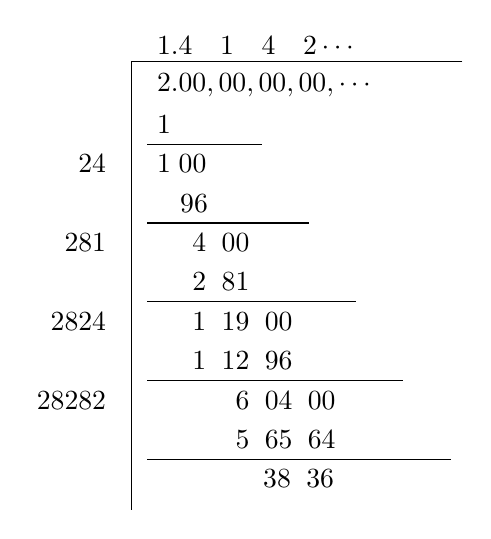
\begin{tikzpicture}[scale=2]
\node at (0,0)[right]{$\qquad \quad\;\;\;  38\;\;36$};
\node at (0,0.25)[right]{$\qquad\;\;\;  5\;\;65\;\;64$};
\node at (0,0.5)[right]{$\qquad \;\;\; 6\;\;04\;\;00$};
\node at (0,0.75)[right]{$\quad \; 1\;\;12\;\;96$};
\node at (0,1)[right]{$\quad \; 1\;\;19\;\;00$};
\node at (0,1.25)[right]{$\quad\; 2\;\;81$};
\node at (0,1.5)[right]{$\quad \; 4\;\;00$};
\node at (0,1.75)[right]{$\;\;\; 96$};
\node at (0,2)[right]{$1\;00$};
\node at (0,2.25)[right]{$1$};
\node at (0,2.5)[right]{$2.00,00,00,00,\cdots$};
\node at (0,2.75)[right]{$1.4\quad1\quad4\quad2\cdots$};
\draw(2,2.65)--(-0.1,2.65)--(-0.1,-.2);

\foreach \x/\xtext in {2/24,1.5/281,1/2824,.5/28282}
{
   \node at (-.2,\x)[left]{\xtext};
}

\foreach \x in {2.125,1.625,...,0.125}
{
    \draw (0,\x)--(2-.6*\x,\x);
}
\end{tikzpicture}
\end{center}

从计算中知道
\[1.4142<\sqrt{2}<1.4143\]
\[|\sqrt{2}-1.4142|<\frac{1}{10^4}, \qquad |\sqrt{2}-1.4143|<\frac{1}{10^4}\]

因此,1.4142, 1.4143 分别是 $\sqrt{2}$ 的精确到 $\dfrac{1}{10^4}$ 的不足近似值与过剩近似值。

\medskip
总结上面对于逼近法的讨论,我们得到了下列几点简要的初步认识:
\begin{enumerate}
    \item 实数系,有理数系,整数系,自然数系的包含关系是这样的:
\[\begin{split}
    &\qquad \mathbb{R}\quad \supset \quad \mathbb{Q}\quad \supset \quad \mathbb{Z}\quad \supset \quad \mathbb{N}\\
    &\text{实数系\quad 有理数系\quad 整数系\quad 自然数系}
\end{split}
\]

实数系还包括无理数,任何无理数都可以用有理数去逼近它!二分逼近法和 $q$ 分逼近法是各种逼近法中最常用的几种。
\item 一般说来,逼近法就是对于某一给定实数 $x$ 逐步地去求它的近似值 $a_n$,使得误差 $|x-a_n|$ 可以小到任意小。在 $q$ 分法中,使得误差小到任意小的办法是用逐次$q$ 等分同时求出一个“不足近似值” $a_n$ 和一个“过剩近似值” $b_n$,它们把所要逼近的实数 $x$ 夹逼在当中,即 $a_n<x<b_n$。因为当 $n$ 逐步增大时,$b_n-a_n=\dfrac{b_0-a_0}{q^n}$ 是显然可以小到任意小!这也就是说,给定实数 $x$ 由它的不足近似值数列 $\{a_1,a_2,\ldots ,a_n,\ldots\}$ 和过剩近似值数列 $\{b_1,b_2,b_3,\ldots ,b_n,\ldots \}$ 唯一确定。

\item 更普遍地,对给定的实数 $x$, 用某种方法得到两
个无穷数列 $\{a_1,a_2,\ldots ,a_n,\ldots\}$ 和 $\{b_1,b_2,\ldots ,b_n,\ldots \}$, 它们和 $x$ 之间满足下列关系:
\[a_1\leqslant a_2\leqslant \cdots \leqslant a_n\leqslant \cdots<x<\cdots\leqslant b_n\leqslant \cdots\leqslant b_2\leqslant b_1\]
而且在 $n$ 不断增大时,$(b_n-a_n)$ 可以小到任意小,则 $\{a_n\}$ 就叫做 $x$ 的一个“左逼近数列”,$\{b_n\}$ 就叫做 $x$ 的一个“右逼近数列”,它们分别从左、右夹逼 $x$,这样,$x$ 也就由这两组数列唯一确定。
\end{enumerate}


\subsection{实数系的基本性质}
实数系是计算长度、面积、重量、时间等等这一类量不可缺少的工具。实数系具有四则运和大小次序这两种基本结构。现在我们先以线段的长度为例,从几何上定义实数系的四则运算和大小次序,这样,同学就容易从几何上验证实数(线段长度)满足有理数系的四则运算和大小次序的基本性质。然后,我们将在第七章利用数列极限的概念再给出实数的算术运算的定义。

将两个线段 $AB$, $CD $互相叠置,使 $A$ 点与 $C$ 点重合,如果 $D$ 点不与 $B$ 点重合,落在线段 $AB$ 上,那么线段 $AB$ 的长度 $k$ 个单位就大于线段 $CD$ 的长度 $\ell$ 个单位,记作 $k>\ell$;如果 $D$ 点落在线段 $AB$ 的延长线上,那么线段 $AB$ 的长度就小于线段 $CD$ 的长度,记作$k<\ell$;如果 $D$ 点与 $B$ 点重合则说线段 $AB$ 与 $CD$ 有相等长度,记作$k=\ell$。

我们定义,和 $k+\ell$ 与差 $k-\ell\; (k>\ell )$ 分别是线段的几何和与差的长度。

例如线段 $AB$ 的长度是 $k$ 单位,$BC$ 的长度是 $\ell$ 单位,则线段 $AC$ 的长度就是 $(k+\ell)$ 单位,如\cref{fig:length} 所示。
\begin{figure}
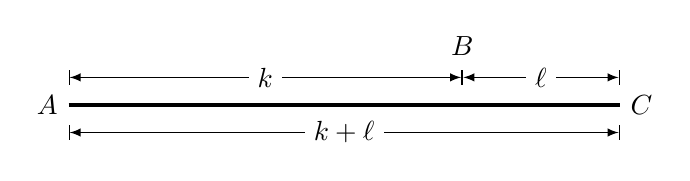
\begin{tikzpicture}[>=latex]
\draw[|<->|] (0,-.35)--node[fill=white]{$k+\ell$}(7,-.35);
\draw[|<->|] (0,.35)--node[fill=white]{$k$}(5,.35);
\draw[|<->|] (5,.35)--node[fill=white]{$\ell$}(7,.35);
\node at (5,.5)[above]{$B$};
\draw[very thick](0,0)node[left]{$A$}--(7,0)node[right]{$C$};

\end{tikzpicture}
    \caption{}\label{fig:length}
\end{figure}

现在我们定义积 $ab$,如\cref{fig:production1},画了一个任意角,在它的一边上,从顶点开始顺次截取长度为 1 和 $b$ 的线段 $OA$ 和 $AC$,在另一边上截取长度为 $a$ 的线段 $OB$,此外,作直线 $CD$ 平行于直线 $AB$,$CD$ 截得的线段 $BD$ 的长度,定义为积 $ab$。这个定义是合理的,因为如果我们在另一个角 $O'$ 上类似地作图(\cref{fig:production2}),那么得到的线段 $B'D'$ 的长度和线段 $BD$ 的长度相等。

\begin{figure}
\begin{minipage}{0.48\linewidth}
  \centering
  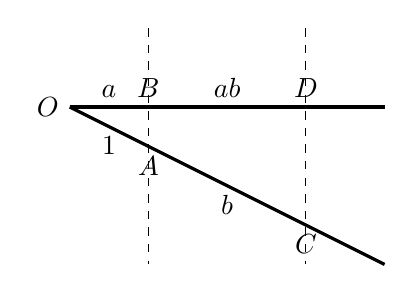
\begin{tikzpicture}
    \draw[very thick] (0,0)node[left]{$O$}--(4,0);
    \draw[very thick] (0,0)--(4,-2);
    \draw[dashed] (1,1)--(1,-2);
    \draw[dashed]  (3,1)--(3,-2);
    \foreach \x/\xtext in {1/B,3/D}
    {
        \node at (\x,0) [above]{$\xtext$};
    }
    \foreach \x/\xtext in {1/A,3/C}
    {
        \node at (\x,-.5*\x) [below]{$\xtext$};
    }
% \node at (2,-2.5){$(1)$};
    \node at (.5,-.25)[below]{1};
    \node at (.5,0)[above]{$a$};
    \node at (2,-1)[below]{$b$};
    \node at (2,0)[above]{$ab$};
  \end{tikzpicture}
  \subcaption{}\label{fig:production1}
\end{minipage}
\begin{minipage}{0.48\linewidth}
  \centering
  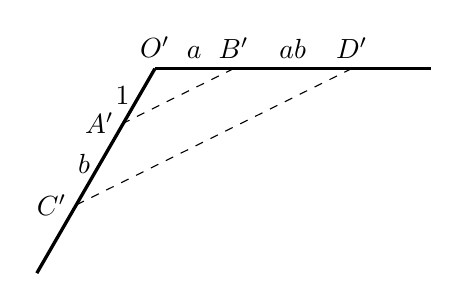
\begin{tikzpicture}
    \draw[very thick] (0,0)node[above]{$O'$}--(3.5,0);
    \draw[very thick] (0,0)--(-120:3);
    \draw[dashed]  (1,0)node[above]{$B'$}--(-120:.8)node[left]{$A'$};
    \draw[dashed]  (2.5,0)node[above]{$D'$}--(-120:2)node[left]{$C'$};
    \node at (.5,0)[above]{$a$};
    \node at (-120:1.4)[left]{$b$};
    \node at (3.5/2,0)[above]{$ab$};
    \node at (-120:.4)[left]{$1$};
  \end{tikzpicture}
  \subcaption{}\label{fig:production2}
\end{minipage}
    \caption{}
\end{figure}

除法运算定义为乘法的逆运算。如\cref{fig:division}, 在角的一边上从顶点开始,顺次截取长度为 $b$ 和 $a$ 的线段,而在另一边上截取单位线段,作 $CD$ 平行于 $AB$, 于是 $AC$ 的长度定义为 $\dfrac{a}{b}$ 这个定义也是合理的,并且 $b\left(\dfrac{a}{b}\right)=a$。

\medskip
最后,我们来规定负长度和零长度。在数轴上,原点 $O$ 右边的点和这点与点 $O$ 的连接线段的长度成一一对应,我们把这种长度称为正的长度。我们把直线上关于原点 $O$ 和点$A$ (即对应长度为 $a$ 的点)对称的点 $A'$ 的相应线段的长度,形式地规定为负的长度 $-a$, 规定点 $O$ 对应于长度零。结果在整个直线上的点和实数之间建立了一一对应。

现在从几何上容易验证实数在四则运算和大小次序这两种结构上满足下面的基本性质,例如,用\cref{fig:distributive_law} 可以验证分配律 $a(b+c)=ab+ac$。

\begin{figure}[htp]
    \begin{minipage}[t]{0.48\textwidth}
    \centering
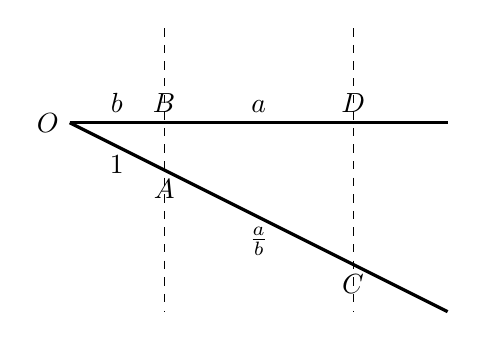
\begin{tikzpicture}[>=latex, scale=1.2]
    \draw[very thick] (0,0)node[left]{$O$}--(4,0);
    \draw[very thick] (0,0)--(4,-2);
    \draw[dashed] (1,1)--(1,-2);
    \draw[dashed]  (3,1)--(3,-2);
    \foreach \x/\xtext in {1/B,3/D}
    {
        \node at (\x,0) [above]{$\xtext$};
    }
    \foreach \x/\xtext in {1/A,3/C}
    {
        \node at (\x,-.5*\x) [below]{$\xtext$};
    }

\node at (.5,-.25)[below]{1};
\node at (.5,0)[above]{$b$};
\node at (2,-1)[below]{$\frac{a}{b}$};
\node at (2,0)[above]{$a$};   
    \end{tikzpicture}
    \caption{}\label{fig:division}
    \end{minipage}
    \begin{minipage}[t]{0.48\textwidth}
    \centering
    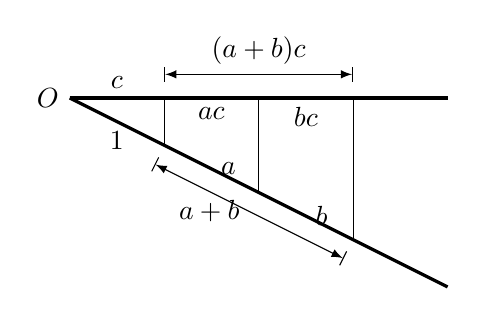
\begin{tikzpicture}[>=latex, scale=1.2]
 \draw[very thick] (0,0)node[left]{$O$}--(4,0);
    \draw[very thick] (0,0)--(4,-2);
    \draw (1,0)--(1,-.5);
    \draw  (2,0)--(2,-1);
    \draw  (3,0)--(3,-1.5);
\node at (.5,-.25)[below]{1};
\node at (.5,0)[above]{$c$};
\node at (1.5,0)[below]{$ac$};   
\node at (2.5,0)[below]{$bc$};   
\node at (1.5,-0.75)[right]{$a$};   
\node at (2.5,-1.25)[right]{$b$};  
\draw[|<->|] (1,.25)--node[above]{$(a+b)c$}(3,.25);
\draw[|<->|] (1-.1,-.5-.2)--node[left]{$a+b$}(3-.1,-1.5-.2);
    \end{tikzpicture}
    \caption{}\label{fig:distributive_law}
    \end{minipage}
    \end{figure}

\subsubsection{加法和乘法的运算性质}

\begin{enumerate}
  \item 交换律:$a+b=b+a;\qquad  ab=ba$
  \item 结合律:$(a+b)+c=a+(b+c);\qquad (a\cdot b)\cdot c=a\cdot (b\cdot c)$
  \item 分配律:$a\cdot (b+c)=a\cdot b+a\cdot c$
  \item 可逆性:$a+x=b;\qquad a\cdot x=b\; (a\ne 0)$ 都是唯一可解的,第一式的解是 $b-a$;第二式的解是 $b/a$。
\end{enumerate}

\subsubsection{顺序性}
\begin{enumerate}
  \item 对于任意实数 $a,b$, 下列关系中有一种且仅有一种成立:
  \[a>b,\qquad a=b\quad \text{或}\quad a<b\]
  \item 由$a<b$和$b<c$推出$a<c$(符号“$<$”的传递性)。
  \item 设$a<b$则$a+c<b+c$
  \item 符号定则
  \[\begin{cases}
      a>0,\qquad b>0\\
      a>0,\qquad b<0\\
      a<0,\qquad b<0
  \end{cases}\Rightarrow\quad  \begin{cases}
      a\cdot b>0\\a\cdot b<0\\a\cdot b>0\\
  \end{cases}\]
  \item 对于任意两个正实数,$a,b>0$, 恒存有一够大的正整数 $n$, 使得 $na<b$。 (通常称之为阿基米德性质)
\end{enumerate}

\subsubsection{ 实数集连续性(完备性)}
我们已经知道实数系与有理数系在加、乘及不等式的运算上有完全相同的性质,但是实数系还具有一个有理数系所没有的优良性质,那就是下面讨论的实数系连续性(完备性)。

在前面,我们用二分法和十分法为例,说明了任何给定的实数 $x$ 都可以用有理数去逼近它。我们所用的是两个有理数列 $\{a_n\}$ 和 $\{b_n\}$ 从左、右夹逼 $x$,$\{a_n\}$,$\{b_n\}$ 和 $x$ 之间的关系可以用下面这一串次序关系来表达:
\[a_1\leqslant a_2\le\cdots\leqslant a_n\leqslant \cdots <x<\cdots\leqslant b_n\leqslant \cdots\leqslant b_2\leqslant b_1\]
$(b_n-a_n)$ 可以任意小,记作 $(b_n-a_n)\to 0$。上面是实数 $x$ 已经先给定了的情况,去求出两串数列 $\{a_n\}$ 和 $\{b_n\}$ 来左、右夹逼实数 $x$,也就是说,数轴$\ell$ 上的每一点,即每一个实数,能够由上述的两个有理数列来唯一确定。反过来问,假如先给定了满足下述这样一串大小次序关系的 $\{a_n\}$ 和 $\{b_n\}$,即
\[a_1\leqslant a_2\le\cdots\leqslant a_n\leqslant \cdots \leqslant b_n\leqslant \cdots\leqslant b_2\leqslant b_1\]
且 $(b_n-a_n)$ 可以任意小,是不是会有那么一个实数 $x$ 去被 $\{a_n\}$、$\{b_n\}$ 左、右夹逼呢?上述问题的答案是肯定的!因为从实数系在长度度量的直观上看,这个实数$x$ 的存在也就是说实数轴上没有空隙存在,即直线是连续不断的,换言之,实数系也是连续不断的,因此我们称实数系为\emph{实数连续统};它说明实数系包含着度量时所有应该包含的数,所以也叫做实数系的\emph{完备性}。下面是直线连续不断的直观概念的解析
描述。

\begin{Theorem}[实数系完备性]{性质}
  对于任给满足下述大小次序关系的两个数列 $\{a_n\}$ 和 $\{b_n\}$,即
\[a_1\leqslant a_2\leqslant \cdots a_n\leqslant \cdots \leqslant b_n\leqslant \cdots \leqslant b_2\leqslant b_1\]
且 $(b_n-a_n)\to 0$,则必定存在一个介于所有 $a_n,b_n$ 之间的实数 $x$。
\end{Theorem}

实数系的完备性是非常基本而且重要的!在以后的章节中,我们将用这个性质来证明极限的存在,从而可进行一切极限运算,而这些运算乃是微积分的基础。在每次用到时,我们将详细解说其用法。这样逐步渐近,同学不难学会它的种种用法。

\begin{Exercise}
\begin{question}
  \item 证明 $\sqrt{3}$ 是无理数。
  \item 设 $\sqrt{5}=a$,$a$ 的小数部分用 $b$ 表示,求 $a-\dfrac{1}{b}$。
  \item 若 $a+\sqrt{b}=c+\sqrt{d}$, 这里 $a,b,c,d$ 是有理数而 $\sqrt{b}$ 是无理数,则 $a=c$,$b=d$,试证之。
  \item 利用“整系数方程 $a_0x^n+a_1x^{n-1}+\cdots+a_{n-1}x+a_n=0$ 的任何有理根,如果写成既约分数时为 $\dfrac{p}{q}$,那么分子 $p$ 是 $a_n$ 的约数,分母 $q$ 是 $a_0$ 的约数”,这一准则使我们能够得到一切有理实根,从而证明任何其它根都是无理数。试证明:$3+2\sqrt{2}$,$1+\sqrt[3]{3}$,$\sqrt[3]{2}+\sqrt[3]{4}$ 都是某一整系数方程的无理根,从而证明这些数都是无理数。
  \item 
  \begin{tasks}
    \task 如果 $a$ 是有理数,$x$ 是无理数,试证明 $a+x$ 是无理数;又如果 $a \neq 0$, 试证明 $ax$ 是无理数。
    \task 试证明任何两个有理数之间至少存在着一个无理数,因而存在着无穷多个无理数。
  \end{tasks}
  \item 试证明:任给无理数 $a$ 和正整数 $m$, 我们可以找到分数 $\dfrac{n}{m}$,使得 \[\left|a-\frac{n}{m}\right|<\frac{1}{2m}\]
  \item 若等腰三角形的顶角为 \ang{36},底边长为 1, 试证它的腰长不能用有理数表示。
  \item 用二分逼近法求下列无理数的有理近似值,使得误差小于 $1/100$:
    \begin{tasks}(2)
        \task $\sqrt{7}$
        \task $\sqrt[3]{2}$
    \end{tasks}
\end{question}
\end{Exercise}

\section{不等式与绝对值}
不等式在高等数学中所起的作用要比在初等数学中大得多,一个量 $x$ 的精确值往往难以确定,不过,对 $x$ 进行估值,即指明 $x$ 大于某个已知量 $a$ 而小于另一个已知量 $b$,却是容易做到的。在许多应用中,重要的只是知道 $x$ 的这种估值。为以后学习方便起见,我们要在这一节比较详细地回顾一下不等式的一些重要性质。

\subsection{不等式的性质}
$a$ 和 $b$ 是实数,如果 $a-b>0$,那么就称 $a$ 大于 $b$,记作 $a>b$;如果 $a-b<0$,那么就称 $a$ 小于 $b$,记作 $a<b$;如果 $a-b=0$ 那么就称 $a$ 等于 $b$,记作 $a=b$。注意若 $a<b$ 有时也说成 $b>a$,因此 $a<b$ 和 $b>a$ 是等价的。

应用两个正实数之和或积仍然是正数这个基本事实,即如果 $a>0$ 和 $b>0$ 则有$a+b>0$ 和 $ab>0$,而且依据不等式 $a>b$ 等价于 $a-b>0$,我们容易推导出下面的性质。

\begin{Theorem}{性质1}
  若 $a>b$ 和 $c>d$,则 $a+c>b+d$。换言之,同向的两个不等式可以相加。
\end{Theorem}

\begin{Theorem}{性质2}
  若 $a>b$ 且 $c>0$,则 $ac>bc$。
\end{Theorem}

\begin{Theorem}{性质3}
  若 $a>b$ 且 $c<0$, 则 $ac<bc$。
\end{Theorem}

上面的性质 2 和性质 3 也可以表达为不等式若乘以正数得到同向不等式;若乘以负数则得到异向的不等式。更一般地可以得到:

若 $a>b>0$ 和 $c>d>0$ 则 $ac>bd$。也就是两个同向的正数不等式可以相乘。
\begin{Theorem}{性质4}
  \begin{itemize}
    \item 若 $a>b>0$, 则 $1/a<  1/b$;
    \item 若 $a>0>b$, 则 $1/a>0>1/b$;
    \item 若 $a<b<0$, 则 $1/a>  1/b$。
  \end{itemize}
\end{Theorem}   

\begin{Theorem}{性质5}
  若 $a>b$ 而 $b>c$, 则 $a>c$。
\end{Theorem}

这就是说不等式具有传递性,在几何上这是显然的,也可由 $(a-b)+(b-c)=a-c$ 为正直接推出,在上述推演中,如果我们处处都用符号 $\geqslant $ 代替 $>$,则各项法则仍然成立。

\begin{Theorem}{性质6}
  若 $a>b>0$, 则 $a^2>b^2$。
\end{Theorem}

我们注意到 $a^2-b^2=(a+b)(a-b)$, 因为 $a+b$ 是正数,由 $a>b$ 可以推出,$a^2>b^2$。这样正数之间不等式可以进行平方运算。

\begin{Theorem}{性质7}
  若 $a>b>0$, 则 $\sqrt{a}>\sqrt{b}$,即在正实数之间的不等式两端能取平方根。
\end{Theorem}

事实上,$\sqrt{a}-\sqrt{b}=\dfrac{a-b}{\sqrt{a}+\sqrt{b}}$,因为 $\sqrt{a}+\sqrt{b}$ 是正数,从而由 $a>b$ 就可推出 $\sqrt{a}-\sqrt{b}>0$, 即$\sqrt{a}>\sqrt{b}$。

更一般地,若 $a>b>0$ 且 $n$ 是自然数,那么 $a^n>b^n$。

这个结论可以用数学归纳法来证明。这个证明留给同学作为练习。

\medskip
反过来,若 $a>b>0$, 且 $n$ 是一个正整数,则 $a^{\frac{1}{n}}>b^{\frac{1}{n}}$。

\begin{proof}
\linespread{1.5}\selectfont
假设 $a^{\frac{1}{n}}=b^{\frac{1}{n}}$,那么$\Big(a^{\tfrac{1}{n}}\Big)^n>\Big(b^{\tfrac{1}{n}}\Big)^n$,因而,$a=b$,这就与已知 $a>b$ 矛盾。

假设 $a^{\frac{1}{n}}<b^{\frac{1}{n}}$,于是 $\Big(a^{\tfrac{1}{n}}\Big)^n<\Big(b^{\tfrac{1}{n}}\Big)^n$,即 $a<b$,这又与已知条件 $a>b>0$ 矛盾,故我们得出结论 $a^{\tfrac{1}{n}}>b^{\tfrac{1}{n}}$。\par
\end{proof}

\subsection{绝对值不等式}
我们回想到$|x|$的定义是这样的:

\begin{Definition}%{定义}
$x$ 是一个实数,当 $x$ 是一个非负数时,$x$ 的绝对值 $|x|$ 是它本身;当 $x$ 是一个负数时,$x$ 的绝对值 $|x|$ 是 $x$ 的相反数。
\begin{equation}
|x|=\begin{cases}
    x,&x\geqslant 0\\
    -x,&x<0
\end{cases}
\end{equation}
\end{Definition}

我们也可以说,当 $x$ 不为零时,$|x|$ 是 $x$ 和 $-x$ 两数之中的较大者;当 $x$ 为零时,$|x|$ 则等于二者之中任何一个。即
\begin{equation}
  \begin{split}
    |x|&=\max\{x,-x\},\qquad (x\ne 0)\\
    |x|&=x=-x,\qquad (x=0)
  \end{split}
\end{equation}

\begin{example}
\[|5|=\max\{5,-5\}=5,\qquad |-5|=\max\{5,-5\}=5,\qquad |0|=0\]
\end{example}

\subsubsection{$|x|$ 的几何意义}
在 $Oxy$ 平面内,$P(x,0)$ 和原点 $O(0,0)$ 之间的距离是
\[d=\sqrt{(x-0)^2+(0-0)^2}=\sqrt{x^2}=|x|\]
因此我们可以说 $|x|$ 是 $P(x,0)$ 点离开原点有 $x$ 单位的\emph{距离}。

\cref{fig:distance} 说明 $|x_2|=|P_2O|$, $|x_1|=|OP_1|$, 其中 $x_2<0$,
$x_1>0$。
\begin{figure}
 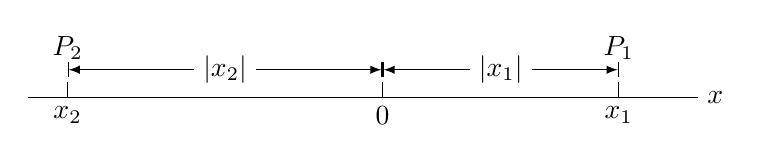
\begin{tikzpicture}[>=latex]
\draw(-.5,0)--(8,0)node[right]{$x$};
\foreach \x/\xtext in {0/x_2,4/0,7/x_1}
{
    \draw (\x,0)node[below]{$\xtext$}--(\x,.2);
}
\draw[|<->|](0,.35)node[above]{$P_2$}--node[fill=white]{$|x_2|$}(4,.35);
\draw[|<->|](7,.35)node[above]{$P_1$}--node[fill=white]{$|x_1|$}(4,.35);

 \end{tikzpicture}
    \caption{}\label{fig:distance}
\end{figure}

如果我们要在 $x$ 轴上描述距离原点不超过 2 个单位的点集,我们把这个条件可以直接写成
\begin{equation}
  \label{eq:abs_neq}
    |x|\leqslant 2
\end{equation}
这个不等式的解集是位于以原点 $O$ 为中心,长度等于 4 的线段上的一切点。\cref{fig:range} 说明这些点的位置。
\begin{figure}
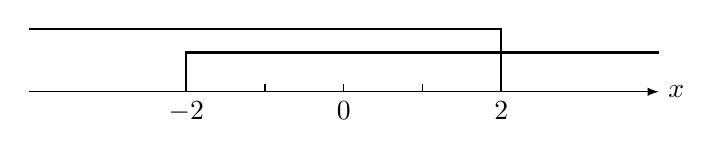
\begin{tikzpicture}[>=latex]
    \draw[->](-4,0)--(4,0)node[right]{$x$};
    \foreach \x in {-2,0,2}
    {
        \draw(\x,0)node[below]{$\x$}--(\x,.1);
    }
    \draw[thick] (-2,0)--(-2,.5)--(4,.5);
    \draw[thick] (2,0)--(2,.8)--(-4,.8);
    \foreach \x in {-1,1}
    {
        \draw(\x,0)--(\x,.1);
    }
\end{tikzpicture}
    \caption{}\label{fig:range} 
\end{figure}

从上面看出这些点的坐标满足不等式
\begin{equation}
  \label{eq:range_neq}
    -2\leqslant x\leqslant 2
\end{equation}
这就是说\cref{eq:abs_neq} 和\cref{eq:range_neq} 是等价的不等式。今后我们将经常遇到的不等式具有下面的形式
\begin{equation}
  \label{eq:abs_neq2}
    |x-a|<3
\end{equation}

$|x-a|=\sqrt{(x-a)^2}$ 的几何意义是 $x$ 轴上的 $P(x,0)$ 点离开 $A(a,0)$ 点的距离。因此已给的不等式是描述在 $x$ 轴上距离 $A(a,0)$ 点小于 3 个单位的点集,根据上面的例题的结论,\cref{eq:abs_neq2} 等价于 $-3<x-a<3$。

不等式的各端加 $a$,得到
\begin{equation}
  a-3<x<a+3    
\end{equation}

因此满足不等式 \eqref{eq:abs_neq2} 的点的坐标是在 $a-3$ 与 $a+3$ 之间(不包括 $a-3$ 和 $a+3$)。

\begin{example}
  在 $x$ 轴上哪些点满足不等式 $|x-3|\leqslant 5$。
\end{example}

\begin{solution}
  $|x-3|\leqslant 5$, 即 $-5\leqslant x-3\leqslant 5$,也即
\[-5+3\leqslant x\leqslant 5+3\]
$\therefore\quad -2\leqslant x\leqslant 8$

这些点位于以 3 为中心,长度等于 10 个单位的线段上,见\cref{fig:solution}。
\begin{figure}
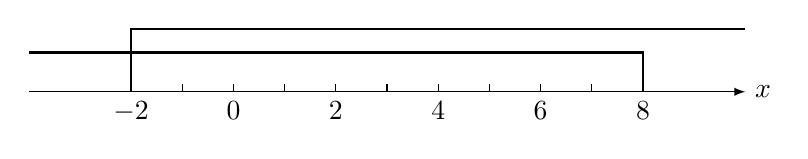
\begin{tikzpicture}[>=latex, xscale=1.3]
    \draw[->](-2,0)--(5,0)node[right]{$x$};
    \foreach \x in {-2,0,2,...,8}
    {
        \draw(\x/2,0)node[below]{$\x$}--(\x/2,.1);
    }
    \foreach \x in {-1,1,...,7}
    {
        \draw(\x/2,0)--(\x/2,.1);
    }
    \draw[thick] (-1,0)--(-1,.8)--(5,.8);
    \draw[thick] (4,0)--(4,.5)--(-2,.5);
\end{tikzpicture}

    \caption{}\label{fig:solution}
\end{figure}

同样地,我们也可以解释 $x>3$ 的几何意义,不等式 $|x|>3$ 是描述在 $x$ 轴上距离原点大于 3 个单位的点集,\cref{fig:solution2} 说明了这些点的位置,图中的圆圈表示去掉 $\pm 3$,因此这些点的坐标小于 $-3$ 或大于 3,即
\[x<-3,\quad \text{或}\quad x>3\]

\begin{figure}
\begin{tikzpicture}[>=latex]
    \draw[->](-4,0)--(4,0)node[right]{$x$};
    \foreach \x in {-3,0,1,3}
    {
        \draw(\x,0)node[below]{$\x$}--(\x,.1);
    }
    \foreach \x in {-2,-1,...,2}
    {
        \draw(\x,0)--(\x,.1);
    }
    \draw[thick] (-3,0)--(-3,.5)--(-4,.5);
    \draw[thick] (3,0)--(3,.5)--(4,.5);
    \foreach \x in {-3,3}
    {
        \draw (\x,0) [fill=white]circle(1.5pt);
    }
\end{tikzpicture}
    \caption{}\label{fig:solution2}
\end{figure}

这就是说,不等式 $|x|>a\; (a>0)$ 等价于不等式 $x<-a$ 或 $x>a\; (a>0)$。
\end{solution}


\begin{example}
  求满足不等式 $(x+2)^2-16>0$ 的点集。
\end{example}

\begin{solution}
  移项
  \[(x+2)^2>16\]
  两边开平方,等价于
  \[|x+2|>4\]
  即
  \[\begin{split}
        x+2<-4\qquad &\text{或}\qquad x+2>4\\  x<-6\qquad &\text{或}\qquad x>2
  \end{split}\]
因此,满足不等式的解集是 $\{x|x<-6\}\cup\{x|x>2\}$。

利用二次函数 $y=(x+2)^2-16$ 的草图,如\cref{fig:parabolic},就更直接地得到 $x<-6$或$x>2$。
\begin{figure}
\begin{tikzpicture}[>=latex, scale=.5]
    \draw[->](-7,0)--(3,0)node[right]{$x$};
    \draw[->](0,-17)--(0,1)node[right]{$y$}; 
\draw[domain=-6.1:2.1, samples=100, thick] plot(\x,{(\x+2)*(\x+2)-16 });
\foreach \y in {-1,-2,...,-16}
{
    \draw (0,\y)--(-.2,\y);
}
\foreach \x in {-6,-5,...,2}
{
    \draw (\x,0)--(\x,.2);
}
\node at (2.5,0)[below]{$2$};
\node at (-6.5,0)[below]{$-6$};
\node at (.5,-.5){$O$};
\node at (0,-16)[right]{$-16$};
\end{tikzpicture}
    \caption{}\label{fig:parabolic}
\end{figure}
\end{solution}

\subsubsection{和、积、商的绝对值}
若 $a$ 和 $b$ 是实数,则 $a\leqslant |a|$ 和 $b\leqslant |b|$,相加得到
\[a+b\leqslant  |a|+|b|\]
同样
\[-a\leqslant |a|\qquad \text{和}\qquad -b\leqslant |b|\]
于是
\[-a-b\leqslant |a|+|b|\]
因为 $a+b$ 和 $-(a+b)$ 都不大于 $|a|+|b|$,所以这两个数中最大者也不大于$|a|+|b|$,于是
\[|a+b|=\max\{a+b,-(a+b)\}\leqslant |a|+|b|\]
这个结果
\begin{equation}
    |a+b|\leqslant |a|+|b|
\end{equation}
常叫做\emph{三角不等式},因为它类似于三角形中任何一边小于其它两边之和这个定理。

有时,我们需要 $|a+b|$ 的下限估值,注意到
\[|a|=|(a+b)-b| \leqslant |a+b| +|-b| =|a+b| +|b|\]
因此下面不等式成立
\begin{equation}
  |a+b|\geqslant |a|-|b|
\end{equation}

若 $a,b$ 是任何实数,则
\[|ab|=\sqrt{(ab)^2}=\sqrt{a^2b^2}=\sqrt{a^2}\cdot \sqrt{b^2}=|a|\cdot |b|\]
即
\begin{equation}
  |ab|=|a|\cdot |b|
\end{equation}
\[\left|\frac{a}{b}\right|=\sqrt{\left(\frac{a}{b}\right)^2}=\sqrt{\frac{a^2}{b^2}}=\frac{\sqrt{a^2}}{\sqrt{b^2}}=\frac{|a|}{|b|}\]
即
\begin{equation}
    \left|\frac{a}{b}\right|=\frac{|a|}{|b|}
\end{equation}


\begin{Exercise}
\begin{question}
  \item 解不等式组:
    \[\begin{cases}
      \dfrac{x}{2}-\dfrac{x}{3}>-1\\
      2(x-3)-3(x-2)<0
    \end{cases}\]
  \item 解不等式:
  \begin{tasks}(2)
      \task $|2x-1|<2|1-2x|-3$
      \task $|x+1|+|x-5|>3$
      \task $\left|\dfrac{3x}{x+1}-3\right|<0.01$
      \task $\dfrac{3x-1}{x-5}<2$
  \end{tasks}
  \item 图示满足下面不等式组的点 $(x,y)$的区域 $R$。
  \[\begin{cases}
      |x-1|+|y-5|<1\\
  y>5+|x-1|
  \end{cases}\]
  \item 试证明若 $ax^2+bx+c>0$ 对于任何 $x$ 都成立的充要条件是 $a>0$ 且 $b^2-4ac<0$。
  \item 等差数列与等比数列的首项相等且第 $2n+1$ 项也相等,问第 $n+1$ 项如何?
  \item 若 $x+2y=1$, 求 $xy$ 的最大值。
  \item 平移 $y=-\dfrac{1}{3}x^2$ 使其顶点在抛物线 $y=x^2$ 上,试求这样得到任何一条抛物线都不能经过的范围,并画图表示。
  \item 求证
  \begin{tasks}
    \task $|a+b+c|\leqslant |a|+|b|+|c|$
    \task $|a-b-c|\geqslant |a|-|b|-|c|$
    \task $\Big| |a|-|b| \Big|\leqslant |a+b|$
  \end{tasks}
  \item \begin{tasks}
    \task 若 $|h|<\frac{\varepsilon}{4}$,$|k|<\frac{\varepsilon}{6}$,求证 $|2h-3k|<\varepsilon$。
    \task 若 $|a_n-r|<\varepsilon$,$|a_n-a_n'|<\varepsilon$,求证 $|a_n'-r|<\varepsilon$。
    \task 若 $|b_n|<\varepsilon$,$|a_n-b_n|<\varepsilon$,求证 $|a_n|<2\varepsilon$。
  \end{tasks}
  \item 试用 $a$ 表出从点 $(0,a)$ 到曲线 $y=\left|\frac{x^2}{2}-1\right|$ 上的点 $(x,y)$ 的距离的最小值 $(a>1)$。
  \item 解不等式 $\sqrt{2x^2-3x-2}>x-1$。
\end{question}
\end{Exercise}

\subsection{几个重要的不等式}
下面我们来推导几个常用的著名不等式。

\begin{example}\label{exp:bernoulli}
  贝努利不等式。若 $n\in\mathbb{N}$且$n\geqslant 2$, $a>-1$ 且 $a \neq 0$(即 $a>0$ 或 $-1<a<0$ ),则
\[(1+a)^n>1+na\]
\end{example}

\begin{proof}
\begin{enumerate}
  \item 对于 $n=2$, 因为 $(1+a)^2=1+2a+a^2$,又 $a^2>0$,故不等式成立。
  \item 假设不等式对于 $n=k$ 成立,即
  \[(1+a)^k>1+ka\]
  我们来证明不等式对于 $n=k+1$ 也成立,就是说
  \[(1+a)^{k+1}>1+(k+1)a\]

  事实上,由假设 $1+a>0$,故不等式
  \[(1+a)^k(1+a)>(1+ka)(1+a)\]
  成立,即
  \[(1+a)^{k+1}>1+(k+1)a+ka^2\]
  将上面不等式右边舍去正项 $ka^2$,就知道
  \[(1+a)^{k+1}>1+(k+1)a\]
  成立,因此命题对于 $n\geqslant 2$ 的自然数成立。
\end{enumerate}
\end{proof}

\begin{example}
  无论多少个正数的几何平均数不大于其算术平均数,即
\[\frac{a_1+a_2+\cdots+a_n}{n}\geqslant \sqrt[n]{a_1a_2\cdots a_n}\]
\end{example}

\begin{proof}
令 $A=\dfrac{a_1+a_2+\cdots+a_n}{n}$,则题意是说,
\begin{equation}
  \label{eq:avg_proof}
  A^n\geqslant a_1a_2\cdots a_n
\end{equation}
当 $a_1=a_2=\cdots= a_n$ 时,则\cref{eq:avg_proof} 显然成立。如果 $a_1,a_2,\ldots,a_n$ 这 $n$ 个数有不相等的,由于
    \[nA=a_1+a_2+\cdots+a_n\]
即:
\[(a_1-A)+(a_2-A)+\cdots+(a_n-A)=0\]
则必有一大于 $A$, 也必有一小于 $A$, 不妨设 $a_1>A>a_2$,于是,$A-a_1<0$,$A-a_2>0$,把 $a_1,a_2,\ldots,a_n$ 改换成
\begin{equation}
  \label{eq:new_series}
a_1'=A,\; a_2'=a_2+a_1-A,\; a_3'=a_3,\; \ldots, a_n'=a_n
\end{equation}
由此可见我们新得之 $n$ 个数,其和不变,即
\[\begin{split}
    a'_1+a'_2+\cdots +a'_n&=A+(a_2+a_1-A)+a_3+\cdots +a_n\\
&= a_1+a_2+\cdots +a_n\\
&=nA
\end{split}\]
但其积增大,因为
\[\begin{split}
    A(a_2+a_1-A)-a_1a_2&=Aa_2+Aa_1-A^2-a_1a_2\\
&=A(a_2-A)+a_1(A-a_2)\\
&=(A-a_2)(a_1-A)>0
\end{split}\]
从而
\[A(a_2+a_1-A)a_3\cdots a_n>a_1a_2\cdots a_n\]
若\cref{eq:new_series} 中还有不等于 $A$ 的,比如,$a_s>A>a_m$,我们用同法即用 $A$ 取代其中较大的一个 $a_c$,用 $a_m+a_s-A$ 代换 $a_m$,又可另得 $n$ 个正数,其和同前,而其积更大。由此以往,不过 $n-1$ 次,便可得 $n$ 个相等之正数$\underbrace{A,A,\cdots A}_{\text{$n$个}}$,此时积最大,故有
\[A^n\geqslant a_1a_2\cdots a_n\]
且当 $a_1=a_2=\cdots =a_n$ 时,等式成立。
\end{proof}

\begin{example}\label{exp:Cauchy}
  柯西不等式,若 $a_i,b_i,\; i=1,2,\cdots ,n$ 是实数,则
\[(a_1b_1+a_2b_2+\cdots +a_nb_n)\leqslant (a_1^2+a_2^2+\cdots +a_n^2)(b_1^2+b_2^2+\cdots+b_n^2)\]
当且仅当
$\dfrac{a_1}{b_1}=\dfrac{a_2}{b_2}=\cdots=\dfrac{a_n}{b_n}$ 时,等式成立。
\end{example}

\begin{proof}
对于任何实数 $t$, 不等式
\begin{equation}
  \label{eq:cauchy_binom}
  (a_1+tb_1)^2+(a_2+tb_2)^2+\cdots +(a_n+tb_n)^2\geqslant 0
\end{equation}
成立,将\cref{eq:cauchy_binom} 的左端改写成按 $t$ 的降幂排列,得
\begin{equation}
  \label{eq:cauchy_binom2}
   ( b^2_1+b^2_2+\cdots +b^2_n)t^2+2(a_1b_1+\cdots +a_nb_n)t+(a^2_1+a_2^2+
+\cdots +a_n^2)\geqslant 0
\end{equation} 
设 $A=a^2_1+\cdots +a_n^2$,$B=a_1b_1+\cdots +a_nb_n$,$C=b^2_1+\cdots +b^2_n$,
于是\cref{eq:cauchy_binom2} 写成 $Ct^2+2Bt+A>0$,其中 $C\geqslant 0$。
\begin{itemize}
  \item 若 $C=0$, 于是 $b_1=b_2=\cdots =b_n=0$,显然,柯西不等式成立。
  \item 若 $C>0$,因而 
  \[C\left(t+\frac{B}{C}\right)^2+\left(A-\frac{B^2}{C}\right)\geqslant 0\]
  对于任意实数 $t$ 成立。故令 $t=-\dfrac{B}{C}$ 代入,得到
  \[A-\frac{B^2}{C}\geqslant 0,\qquad \text{即}\qquad \frac{AC-B^2}{C}\geqslant 0\]
  $\because\quad C>0,\qquad \therefore\quad B^2\leqslant AC$, 即
\[(a_1b_1+\cdots +a_nb_n)^2\leqslant (a^2_1+\cdots +a^2_n)(b^2_1+\cdots +b^2_n)\]
再由\cref{eq:cauchy_binom} 推知当且仅当 $-t=\dfrac{a_1}{b_1}=\dfrac{a_2}{b_2}=\cdots=\dfrac{a_n}{b_n}$ 时,等式成立。
\end{itemize}
\end{proof}

\begin{example}
  设 $a_1,a_2,\ldots,a_n,b_1,b_2,\ldots,b_n$ 是实数,则
\[\sqrt{\sum^n_{i=1}(a_i+b_i)^2}\leqslant \sqrt{\sum^n_{i=1}a^2_i}+\sqrt{\sum^n_{i=1}b^2_i}\]
\end{example}

\begin{proof}
 \[   \sum^n_{i=1}(a_i+b_i)^2=\sum^n_{i=1}a_i^2+2\sum^n_{i=1}a_ib_i+\sum^n_{i=1}b_i^2\]
由\cref{exp:Cauchy} 柯西不等式知
\[\sum^n_{i=1}a_ib_i\le\left|\sum^n_{i=1}a_ib_i\right|\leqslant \sqrt{\sum^n_{i=1}a_i^2}\sqrt{\sum^n_{i=1}b_i^2}\]
因此:
\[\begin{split}
    \sum^n_{i=1}(a_i+b_i)^2&\leqslant \sum^n_{i=1}a_i^2+2\sqrt{\sum^n_{i=1}a_i^2}\sqrt{\sum^n_{i=1}b_i^2}+\sum^n_{i=1}b_i^2\\
    &=\left(\sqrt{\sum^n_{i=1}a^2_i}+\sqrt{\sum^n_{i=1}b^2_i}\right)^2
\end{split}\]
两边开平方,取算术根即得所证。
\end{proof}    

% \section*{习题6.3}
% \addcontentsline{toc}{subsection}{习题6.3}
\begin{Exercise}
\begin{question}
   \item  若 $a,b,c,d$ 是不相等正数,求证:
\begin{tasks}
    \task $\displaystyle \frac{b}{a}+\frac{c}{b}+\frac{d}{c}+\frac{a}{d}>4$
    \task $\displaystyle \frac{b}{\sqrt{a}}+\frac{a}{\sqrt{b}}>\sqrt{a}+\sqrt{b}$
\end{tasks}
   \item  若 $a_1,a_2$ 表示正数,$p,q$ 表示正整数,求证:
\begin{tasks}
    \task $\displaystyle a_1^{p+q}+a_2^{p+q}\geqslant a_1^pa_2^q+a_1^qa_2^q$
    \task $\displaystyle \frac{a_1^{p+q}+a_2^{p+q}}{2}\geqslant \left(\frac{a_1^p+a_2^p}{2}\right)\left(\frac{a_1^q+a_2^q}{2}\right)$
\end{tasks}

\item 用数学归纳法证明:
若 $a_1>0$,$a_2>0$,$n$ 是正整数,则
\[\frac{a_1^n+a_2^n}{2}\geqslant \left(\frac{a_1+a_2}{2}\right)^n\]
\item 求证,当 $n$ 是 1 或不小于 5 的自然数时,总有 $2^n>n^2$。
\item 设 $0<a<1$,$0<x_0<1$,$x_n=a(1-x_{n-1})+(1-a)x_{n-1},\quad (n=1,2,3,\ldots)$,
\begin{tasks}
  \task 用 $a$ 与 $x_0$ 表示 $x_n$;
  \task 证明 $0<x_n<1$。
\end{tasks}

\item 设 $a>2$,给定数列 $\{x_n\}$,其中$x_1=a$,$x_{n+1}=\dfrac{x^2_n}{2(x_n-1)},\quad (n=1,2,3,\ldots)$,
求证:
\begin{tasks}
  \task $x_n>2$,且$\dfrac{x_{n+1}}{x_n}<1$;
  \task 如果 $a<3$,那么 $x_n\leqslant 2+\dfrac{1}{2^{n-1}}$。
\end{tasks}

\item 若长方形的体积是定值,求全面积的最小值。
\item 求证球内接长方体中,以正方体的体积为最大。
\item 求证在周长都为 $2L$ 的所有三角形中,面积最大的必是等边三角形。
\item 若 $a,b,c$ 是正数且 $abc=8$。

求证:$\sqrt{a^2+b^2}+\sqrt{b^2+c^2}+\sqrt{c^2+a^2}\geqslant 6\sqrt{2}$

\item 若$a>0$, $b>0$, 且$a+b=1$, 
求证:\[\left(a+\frac{1}{a}\right)\left(b+\frac{1}{b}\right)\geqslant \frac{25}{4}\]

\item 若 $a+b+c=1$, 且 $a>0$, $b>0$, $c>0$, 求证:
\begin{tasks}
    \task $\displaystyle \left(\frac{1}{a}-1\right)\left(\frac{1}{b}-1\right)\left(\frac{1}{c}-1\right)\geqslant 8$
    \task $\displaystyle \frac{1}{a}+\frac{1}{b}+\frac{1}{c}\geqslant 9$
\end{tasks}

\item 若 $x,y$ 是实数,且 $x^2+y^2\leqslant 1$,
求证:$|x^2+2xy-y^2|\leqslant \sqrt{2}$

\item 对于任何实数,求证:
\[\sqrt{\frac{a_1^2+a_2^2+\cdots+a_n^2}{n}}\geqslant \frac{a_1+a_2+\cdots+a_n}{n}\]
当且仅当诸数相等时,等式成立。
\item $a+b=1$, $a>0$, $b>0$, 求证 $\sqrt{2a+1}+\sqrt{2b+1}\leqslant 2\sqrt{2}$。
\item 求证:
\[\frac{|x_1+x_2|}{|4+x_1^2| |4+x_2^2|}<\frac{1}{8}\]
\item 对于 $n\geqslant 2$ 的自然数 $n$, 证明不等式
\[2^n>1+n\sqrt{2^{n-1}}\]
\item 对于任何正整数 $k\leqslant n$, 求证:
\[1+\frac{k}{n}\leqslant \left(1+\frac{1}{n}\right)^k\leqslant 1+\frac{k}{n}+\frac{k^2}{n^2}\]
\item 已知 $a,b,c,d,e$ 是实数,满足
\[a+b+c+d+e=8,\qquad a^2+b^2+c^2+d^2+e^2=16\]
试确定 $e$ 的最大值。
\item 半径为 1 的圆内接三角形面积等于 $\dfrac{1}{4}$,设此三角形三边长为 $a,b,c$,求证:
\begin{tasks}
  \task $abc=13$;
  \task $\sqrt{a}+\sqrt{b}+\sqrt{c}<\dfrac{1}{a}+\dfrac{1}{b}+\dfrac{1}{c}$。
\end{tasks}

\item 直角三角形斜边长等于10, 内切圆半径为$a$。求何
时内切圆的半径最大,最大值是多少?
\item 若$n>2$, 求证$(n!)^2>n^n$。
\item 有$n$个实数$a_1,a_2,\ldots,a_n$且
$a_1+a_2+\cdots+a_n=n$
\begin{tasks}
  \task 求证:$\sqrt{|a_1|}+\sqrt{|a_2|}+\cdots+\sqrt{|a_n|}\geqslant \sqrt{n}$
  \task 又 $a^2_1+a_2^2+\cdots+a^2_n=n$,求 $a_1,a_2,\ldots,a_n$ 的值。
\end{tasks}

\item 若 $a,b,c$ 是正实数,求证:$\dfrac{c}{a+b}+\dfrac{a}{b+c}+\dfrac{b}{c+a}\geqslant \dfrac{3}{2}$。
\end{question}
\end{Exercise}


\chapter{数列的极限}

\section{数列的极限概念}
在前一章中,我们已经看到任何一个实数都可以用有理数来左、右夹逼,即对于任何实数 $x$ 我们总可以用逼近法求得两个有理数列 $\{a_n\}$, $\{b_n\}$ 使得
\[a_1\leqslant a_2\leqslant \cdots \leqslant a_n\leqslant \cdots\leqslant x\leqslant \cdots\leqslant b_n\leqslant \cdots\leqslant b_2\leqslant b_1\]
并且 $b_n-a_n$ 可以小到任意小。

数列中的项 $a_n$ 和 $b_n$ 就是 $x$ 的第 $n$ 次不足近似值和过剩近似值,它们的误差可以用不等式
\[|x-a_n|<b_n-a_n,\qquad |x-b_n|<b_n-a_n\]
来估计。这里所说的逼近的要点在于\emph{误差可以小到任意小},下面用例子从另一个角度来说明这一点。

\medskip
今以 $\dfrac{2}{3}$ 为例,作上述分析:

\medskip
\begin{enumerate}
  \item 以 3 去除 2,得:
    \begin{center}
      \longdivision[2]{2.00}{3}      
    \end{center}
    因为每次 20 除以 3 都余 2, 所以商数 6 重复出现,这个除法可以无止境地作下去。
    \item 上述除式的意义是
\[\begin{split}
    2&=0.6\times3+0.2\Longleftrightarrow 0.6<\frac{2}{3}<0.7,\\
&=0.66\times3+0.02\Longleftrightarrow 0.66<\frac{2}{3}<0.67,\\
&=0.666\times3+0.002\Longleftrightarrow 0.666<\frac{2}{3}<0.667,\\
\cdots 
\end{split}\]
\end{enumerate}

{\linespread{1.6}\selectfont 从上面的分析,同学们可以看出 $\dfrac{2}{3}$ 显然不能用有限位小数表示出,但是存在着由有限位小数所成的无穷数列 $\{a_n\}$ 和 $\{b_n\}$\par}
\[\begin{split}
    \{a_n\}&:\quad a_1=0.6,\; a_2=0.66,\; a_3=0.666,\; \ldots ,\; a_n=0.\underbrace{66\cdots66}_{\text{$n$ 位小数}},\; \ldots\\
    \{b_n\}&:\quad b_1=0.7,\; b_2=0.67,\; b_3=0.667,\; \ldots ,\; b_n=0.\underbrace{66\cdots67}_{\text{$n$ 位小数}},\; \ldots
\end{split}\]
满足 
\[a_n=0.\underbrace{66\cdots66}_{\text{$n$ 位小数}}<\frac{2}{3}<0.\underbrace{66\cdots67}_{\text{$n$ 位小数}}=a_n+\frac{1}{10^n}\]
{\linespread{1.60}\selectfont 并且 $a_n$ 与 $\dfrac{2}{3}$ 之间的误差 $\left|a_n-\dfrac{2}{3}\right|<b_n-a_n=\dfrac{1}{10^n}$, 同样 $b_n$ 与 $\dfrac{2}{3}$ 之间误差 $\left|b_n-\dfrac{2}{3}\right|<\dfrac{1}{10^n}$,只要 $n$ 充分大,误差可以小到任意小。上面的逼近过程,表明无穷数列 $\{a_n\}$, $\{b_n\}$ 从左、右两方面趋近 $\dfrac{2}{3}$,可以使其误差任意小,$\dfrac{2}{3}$ 就是数列 $\{a_n\}$ 的极限,也是数列 $\{b_n\}$ 的极限,用符号表示就是\par}
\[\lim_{n\to\infty}a_n=\frac{2}{3},\qquad \lim_{n\to\infty}b_n=\frac{2}{3}\]
或者用
\[a_n\to \frac{2}{3},\qquad b_n\to\frac{2}{3},\qquad a_n\to \frac{2}{3}\leftarrow b_n\]
来生动地表述上述事实。

{\linespread{1.60}\selectfont 从这里我们看到逼近与极限是密切相关的,极限只是把逼近过程推进到无穷 $(n\to\infty)$ 的结果,逼近只要误差小到所要求的精确度后就可以停止。$\lim\limits_{n\to\infty}a_n=\dfrac{2}{3}$ 表示数列 $\{a_n\}$ 当 $n$ 无限增大的极限值是 $\dfrac{2}{3}$。\par}

{\linespread{1.65}\selectfont
我们再用极限的观点对 $\sqrt{2}$ 进行分析如下。$\sqrt{2}$ 是一个什么数?要回答这个问题,我们只须找出有理数 $\dfrac{a}{b}$ 在什么时候大于 $\sqrt{2}$, 什么时候小于 $\sqrt{2}$,也就是说,如果 $\left(\dfrac{a}{b}\right)^2<2$, 那么正数 $\dfrac{a}{b}<\sqrt{2}$;如果$\left(\dfrac{a}{b}\right)^2>2$, 那么 $\dfrac{a}{b}>\sqrt{2}$。根据有理数是有序的,稠密的,因此有理数的平方总能和 2 比较大小,这就保证我们可以用逼近法(譬如十分逼近法)决定左、右夹逼 $\sqrt{2}$ 的两个由十进位小数组成的数列 $\{a_n\}$、$\{b_n\}$ 如下:\par}
\[\begin{split}
  \{a_n\}&:\quad a_1=1,\; a_2=1.4,\; a_3=1.41,\; a_4=1.414,\ldots\\
  \{b_n\}&:\quad b_1=2,\; b_2=1.5,\; b_3=1.42,\; b_4=1.415,\ldots\\
\end{split}\]
使得 $a_n<\sqrt{2}<b_n$, 而且 $b_n-a_n=\dfrac{1}{10^n}$,于是
\[|a_n-\sqrt{2}|<\frac{1}{10^n},\qquad |b_n-\sqrt{2}|<\frac{1}{10^n} \]
{\linespread{1.6}\selectfont 这就是说,第 $n$ 次的有限小数近似值 $a_n$ 和 $b_n$ 与 $\sqrt{2}$ 的误差分别小于 $\dfrac{1}{10^n}$,因此,只要 $n$ 充分大,误差就可以小到任意小,当我们让这个计算过程,无穷地进行下去时,我们就说 $\sqrt{2}$ 是数列 $\{a_n\}$ 或 $\{b_n\}$ 的极限,记做\par}
\[\lim_{n\to\infty}a_n=\sqrt{2},\qquad \lim_{n\to\infty}b_n=\sqrt{2}\]

从上面两个例子看到,实数是具有 $n$ 位数字的普通十进位小数数列,当 $n$ 无限增大时的极限。

如今我们说明了逼近与极限概念密切相关的一面,但是极限与逼近也有观点不同,概念层次也不同的方面,上面所说用十分逼近法求 $\sqrt{2}$ 的近似值 $1,1.4,1.41,\ldots$ 等是逼近的观点,它是先有 $\sqrt{2}$,即我们先知道 $\sqrt{2}$ 是方程 $x^2=2$
的根,然后用小数去逐步逼近。极限的观点恰恰相反,它是先有一个无穷数列 $\{a_n\}$,然后要去看一下,它们是否恰好无限逼近某一个常数 $A$。假如是这样,就叫 $A$ 是数列 $\{a_n\}$ 的极限值。

下面介绍几个逼近某一常数的无穷数列的例子。

\begin{example}\label{exp:harmonic}
  仔细观察数列:
  \[1,\; \frac{1}{2},\;\frac{1}{3},\;\frac{1}{4},\; \ldots,\;\frac{1}{n},\;\ldots\]
我们马上看出
\begin{enumerate}
    \item 上述数列的每一项都是正数。
    \item 上述数列逐项递减:
\[1>\frac{1}{2}>\frac{1}{3}>\cdots>\frac{1}{n}>\frac{1}{n+1}>\cdots>0\]
因而是一个递减有界数列。
\item\label{itm:cases3} 当 $n$ 愈来愈大时,$a_n=\dfrac{1}{n}$ 愈来愈接近 0, 它们的
误差 $|a_n-0|=\dfrac{1}{n}$, 只要充分大,就可以小到任意小。
\end{enumerate}

对于情形 \ref{itm:cases3},我们就说:数列 $\left\{\dfrac{1}{n}\right\}$ 趋近于 0 或收敛到 0, 或 0 是数列 $\left\{\dfrac{1}{n}\right\}$ 的极限,并记作 $\dfrac{1}{n}\to 0$ 或 $\lim\limits_{n\to\infty}\dfrac{1}{n}=0$。

\medskip
现在,让我们再用数轴把上述事实图解说明如下:
\begin{figure}
    \begin{tikzpicture}[>=latex]
 \draw[->] (-1.5,0)--(10.5,0)node[right]{$\dfrac{1}{n}$};
\foreach \x/\xtext in {1/A_1,.5/A_2,.33/A_3,.25/A_4,.2/A_5,.166/A_6,0/0}
{
    \draw (\x*10,0)node[below]{$\xtext$}--(\x*10,.1);
}
\foreach \x/\xtext in {1/1,.5/\dfrac{1}{2},.33/\dfrac{1}{3},.25/\dfrac{1}{4},.2/\dfrac{1}{5},.166/\dfrac{1}{6},0/0}
{
    \node at (\x*10,.1)[above]{$\xtext$};
}
\node at (-1.2,0){(};
\node at (1.2,0){)};
\node at (-1.2,-.2)[below]{$-\varepsilon$};
\node at (1.2,-.2)[below]{$\varepsilon$};
\draw (.5,0)node[below]{$\cdots A_n$}--(.5,.1)node[above]{$\cdots \dfrac{1}{n}$};
    \end{tikzpicture}
    \caption{}
\end{figure}

在数轴上取以数列:
\[1,\; \frac{1}{2},\;\frac{1}{3},\;\frac{1}{4},\; \ldots,\;\frac{1}{n},\;\ldots\]
的各项为坐标的各点,就得到一个点列:
\[A_1,A_2,A_3,A_4,\ldots,A_n,\ldots,\]
{\linespread{1.6}\selectfont 上述点列 $\{A_n\}$ 从原点 $O$ 的右边逐步向原点逼近,而且其中的点 $A_n$ 到原点的距离 $|a_n-0|=\dfrac{1}{n}$,只要 $n$ 充分大,就可以小到任意小。上面的事实也可以这样来说明:通常我们把 $A$ 点为中心的\emph{开区间} $(A-\varepsilon,A+\varepsilon)$ 叫做这\emph{点 $A$ 的 $\varepsilon$ 邻域}。我们看到,原点 $O$ 的任意$\varepsilon$ 邻域,包含 $\left\{\dfrac{1}{n}\right\}$ 的除有限个点以外的全部点。这也就是说数列 $\left\{\dfrac{1}{n}\right\}$ 是收敛的,并且收敛到 0。\par}
\end{example}

\begin{example}\label{exp:converge}
\linespread{1.6}\selectfont
观察数列 $\displaystyle \left\{\frac{n}{n+1}\right\}: \frac{1}{2},\frac{2}{3},\ldots,\frac{n}{n+1},\ldots$ 同学们容易看出,这个数列逐项递增,其各项 $a_n=\dfrac{n}{n+1}$ 永远小于 1,$a_n$ 和 1 之间的误差 $|a_n-1|=\left|\dfrac{-1}{n+1}\right|=\dfrac{1}{n+1}$,只要 $n$ 充分大就可以到任意小。这也就是说,这个数列在数轴上的对应点列,除有限个点外全部点都在点 1 的任意 $\varepsilon$ 邻域内(\cref{fig:limits}),因此,这个数列 $\left\{\dfrac{n}{n+1}\right\}$ 的极限是 1, 或者变量 $a_n=\dfrac{n}{n+1}$ 的极限是 1,用符号表示就是:
\[\frac{n}{n+1}\to 1,\quad \text{或者}\quad \lim_{n\to\infty}\frac{n}{n+1}=1\]
\begin{figure}
\begin{tikzpicture}[>=latex]
\draw[->] (-.5,0)--(10,0)node[right]{$\frac{n}{n+1}$};
\foreach \x/\xtext in {0/0,.5/\frac{1}{2},.667/\frac{2}{3},.75/\frac{3}{4}, .8/\frac{4}{5},1/1}
{
    \draw (\x*8,0)node[below]{$\xtext$}--(\x*8,.1);
}
\node at (7+.3,0.2)[above]{$1-\varepsilon$};
\node at (9-.3,0.2)[above]{$1+\varepsilon$};
\node at (7+.3,0){(};
\node at (9-.3,0){)};

\end{tikzpicture}  
    \caption{}\label{fig:limits}
\end{figure}
\end{example}

\begin{example}\label{exp:limits}
  \linespread{1.65}\selectfont
  观察数列 $\displaystyle \left(-\frac{1}{2}\right),\; \left(-\frac{1}{2}\right)^2,\; \left(-\frac{1}{2}\right)^3,\ldots,\left(-\frac{1}{2}\right)^n,\;\ldots$, 这个数列逐项正负相间,是摆动数列,显然,各项的绝对值$|a_n|\leqslant\dfrac{1}{2}$,$n=1,2,3,\ldots$,因此,它又是有界的。其第 $n$ 项与数 0 之间的误差 $|a_n-0|=\left(\dfrac{1}{2}\right)^n$,当 $n$ 充分大时,可以小到任意小。再从数轴上看,其对应点列从原点的左、右两侧向原点逼近,而且当 $n$ 充分大时,$a_n$ 全部都在原点的任意 $\varepsilon$ 邻域内(\cref{fig:limits2}),因此,这个数列 $\left\{\left(-\dfrac{1}{2}\right)^n\right\}$ 的极限是 0。
\begin{figure}
 \begin{tikzpicture}[>=latex]
\draw[->] (-5.5,0)--(5.5,0)node[right]{$\left(-\dfrac{1}{2}\right)^n$};
\foreach \x/\xtext in {0/0,-1/-1,-.5/-\dfrac{1}{2},.25/\dfrac{1}{4},1/1}
{
    \draw (\x*5,0)node[below]{$\xtext$}--(\x*5,.1);
}
\foreach \x/\xtext in {0/{},-1/{},-.5/A_1,.25/A_2,1/{}}
{
    \node at (\x*5,.1)[above]{$\xtext$};
}

\foreach \x/\xtext in {-.125/A_3,.0625/A_4}
{
    \draw (\x*5,0)--(\x*5,.1)node[above]{$\xtext$};
}

\foreach \x/\xtext in {-.15/-\varepsilon,.15/\varepsilon}
{
    \node at (\x*5,-.15)[below]{$\xtext$};
}
\node at (-.75,0){(};
\node at (.75,0){)};


 \end{tikzpicture}   
    \caption{}\label{fig:limits2}
\end{figure}
\end{example}

从以上三个数列,我们看到它们的共性是在项数 $n$ 无限增大的过程中,参与在这个过程的变量 $a_n=\dfrac{1}{n}$, $a_n=\dfrac{n}{n+1}$,$a_n=\left(-\dfrac{1}{2}\right)^n$ 所取的值与某一个常数 $A$ 的差的绝对值 $|a_n-A|$(或者说它们之间的绝对误差),只要$n$ 充分大,就可以小到任意小。它们在数轴上对应的点列,只要 $n$ 充分大,除有限个点外全部点都在点 $A$ 的任意 $\varepsilon$ 邻域内。

让我们把只要 $n$ 充分大,误差可以任意小的含义说得更精确些。为此,再以\cref{exp:limits} 说明之,我们来看它的第 $n$ 项与 0 的误差:
\[|a_n-0|=\left|\left(-\frac{1}{2}\right)^n-0\right|=\left(\frac{1}{2}\right)^n\]

当 $n$ 为何值时,$\left(\dfrac{1}{2}\right)^n<0.0001$。解之,得
\[n\lg\left(\frac{1}{2}\right)<-4,\quad \text{即}\quad (-0.3010)n<-4\]
$\therefore\quad n>13.289$

因此,只须 $n\geqslant 14$, 就有
\[|a_n-0|=\left(\frac{1}{2}\right)^n\leqslant \left(\frac{1}{2}\right)^{14}=0.000061<0.0001\]
这也就是说,对于给定的 0.0001, 总能找到这样一个项数,$N=14$, 使得当  $n\geqslant14$ 时,其误差
\[|a_n-0|=\left(\frac{1}{2}\right)^{14}<0.0001\]

当 $n$ 为何值时,$\left(\dfrac{1}{2}\right)^n<\dfrac{1}{10^8}$,只须
\[n\lg\left(\frac{1}{2}\right)<-8\]
即
\[n>\frac{-8}{-0.3010}=26.578\]
因此,只须 $n\geqslant 27$ 时,就有
\[\left(\frac{1}{2}\right)^n<\left(\frac{1}{2}\right)^{27}=0.000000007=7\times 10^{-9}<10^{-8}\]

一般地,任给 $\varepsilon >0$,当 $n$ 为何值时,$\left(\dfrac{1}{2}\right)^n<\varepsilon$。只须
\[n\lg \frac{1}{2}<\lg\varepsilon\] 
即
\[n>\frac{\lg\varepsilon}{-0.3010}\]
由于 $\varepsilon$ 是任意小的正数,当 $\varepsilon <1$ 时,$\lg\varepsilon <0$。于是 $\dfrac{\lg\varepsilon}{-0.3010}$ 是正数,因此,我们总能找到这样项数 $N=\left(\dfrac{\lg\varepsilon}{-0.3010}\text{的整数部分}\right)+1$,使得当 $n\geqslant N$,
\[|a_n-0|=\left(\frac{1}{2}\right)^n<\left(\frac{1}{2}\right)^N<\varepsilon  \]

现在,我们可以给数列 $\{a_n\}$ 的极限是 $A$ 以精确定义如下:

\begin{Definition}
  任给正数 $\varepsilon$, 总可以定出一个正整数 $N$, 使得只要 $n\geqslant N$ 时,$|a_n-A|<\varepsilon$ 都成立,我们就说数列 $\{a_n\}$ 的\emph{极限是} $A$, 或者说数列 $\{a_n\}$ \emph{收敛到} $A$。
\end{Definition}
 
让我们再对上述定义作几点说明:
\begin{enumerate}
  \item $\varepsilon$ (读成 Epsilon)是希腊字母,相当于英文字母的 $e$, 它是 error(误差)的头一个字母,误差任意小的数量提法就是“小于任给正数 $\varepsilon$”。
  \item $a_n$ 是逐步逼近 $A$ 的,要使误差 $|a_n-A|$ 愈小(或者说够小)那就要让数列的项数 $n$ 变得够大,所以“只要 $n\geqslant N$ 时,$|a_n-A|<\varepsilon$”的意义也就是:“只要 $n$ 够大,误差 $|a_n-A|$ 就会小到所要求的那么小!”
  \item $\varepsilon$ 是任给的正数,是变量,但是当误差范围 $\varepsilon$ 一经
给定之后,就为常数,我们对于这个指定的 $\varepsilon$ 检验是否存在
具有上述性质的 $N$, 在求 $N$ 的过程中,$\varepsilon$ 的值不能变动,一般
说来,给的 $\varepsilon$ 愈小,那么求得的 $N$ 愈大。
  \item 定义中的当 $n\geqslant N$ 时,$|a_n-A|<\varepsilon$ 等价于当 $n\geqslant N$ 时,$A-\varepsilon<a_n<A+\varepsilon$ 或 $a_n\in (A-\varepsilon,A+\varepsilon)$,这就是说,如果数列 $\{a_n\}$ 收敛于 $A$ 则在点 $A$ 的任何 $\varepsilon$ 邻域内必包含这个数列的除有限个项以外的一切项。
\end{enumerate}

\medskip
为了帮助同学熟悉极限定义,我们在下面再举几个例子,说明 $N$ 的大小和$\varepsilon$ 之间的关联,并给出证明某数是已知数列的极限的方法。

\begin{example}
  证明数列 $\left\{\dfrac{n}{n+1}\right\}$ 的极限是 1。
\end{example}

\begin{solution}
对于任给 $\varepsilon>0$,要使
\[\left|\frac{n}{n+1}-1\right|=\frac{1}{n+1}<\varepsilon\]
只须 $n+1>\dfrac{1}{\varepsilon}$,即 $n>\dfrac{1}{\varepsilon}-1$,取$N=\left(\frac{1}{\varepsilon}-1\right)$ 的整数部分 $+1$,所以当 $n\geqslant N$ 时,可使
\[\left|\frac{n}{n+1}-1\right|=\frac{1}{n+1}\le \frac{1}{N+1}<\varepsilon\]
这就是说 $\displaystyle\lim_{n\to\infty}\frac{n}{n+1}=1$。
\end{solution}

\begin{example}
  证明数列:$1,0,\dfrac{1}{2},0,\dfrac{1}{3},0,\ldots,0,\dfrac{1}{n},0,\ldots$ 的极限是 0。
\end{example}

\begin{proof}
  这个数列的通项公式可以写成
\[a_n=\begin{cases}
    0,& \text{当 $n$ 为偶数时;}\\
   \dfrac{2}{n+1},& \text{当 $n$ 为奇数时。}
\end{cases}\]

对于任给 $\varepsilon>0$,因为数列 $\{a_n\}$ 的所有偶数项为 0,所以从第二项开始以后的所有偶数项都小于给定的 $\varepsilon$。现在须从奇数项中确定从哪一项开始以后的一切项与 0 的误差小于 $\varepsilon$。 

令奇数项与 0 的误差:$\dfrac{2}{n+1}<\varepsilon$,即
\[n+1>\dfrac{2}{\varepsilon},\qquad n>\dfrac{2}{\varepsilon}-1\]  
取 $N=\left(\dfrac{2}{\varepsilon}-1\right)$ 的整数部分加 1,于是,当 $n\geqslant N$,可使 $\dfrac{2}{n+1}<\varepsilon$。所以对于任给 $\varepsilon>0$, 从第 $N$ 项开始以后的一切项都能使 $|a_n-0|<\varepsilon$ 成立。即 $\lim\limits_{n\to\infty}a_n=0$。
\end{proof}


\begin{example}\label{exp:converge2}
    证明数列 $\left\{\dfrac{n^2-1}{n^2+n+1}\right\}$ 的极限是 1。
\end{example}

\begin{proof}
对于任给 $\varepsilon>0$, 要使
\[|a_n-1|=\left|\frac{n^2-1}{n^2+n+1}-1\right|=\left|\frac{-n-2}{n^2+n+1}\right|=\frac{n+2}{n^2+n+1}<\varepsilon\]
看看是否存在这样的 $N$, 使得当 $n\geqslant N$ 时,永远有 $|a_n-1|<\varepsilon$,
可是直接从上面的不等式解出 $N$ 是不容易的,但我们注意到,当 $n$ 充分大时,在分子中起主导作用的是 $n$,而在分母中起主导作用 $n^2$。如果把分子扩大为 $2n\; (n>2)$, 又把分母缩小为 $n^2$, 这样有 \[|a_n-1|=\frac{n+2}{n^2+n+1}<\frac{2n}{n^2}=\frac{2}{n}\]

现在令 $|a_n-1|<\dfrac{2}{n}<\varepsilon$,即 $n>\dfrac{2}{\varepsilon}$,取 $N$ 为$\dfrac{2}{\varepsilon}$ 的整数部分加 1, 于是,当 $n\geqslant N$ 时,可使
\[|a_n-1|<\frac{2}{n}<\varepsilon\]
这就是说 $\displaystyle\lim_{n\to\infty}\frac{n^2-1}{n^2+n+1}=1$。
\end{proof}

\bigskip
在上面的证明中,所取得的 $N$ 比实际所需要的要大一些,这样并不影响我们所要说明的问题:“$N$ 是根据预先给定的 $\varepsilon$ 来确定的,而且这个 $N$ 满足极限定义中的条件”,事实上,$N$ 不是由 $\varepsilon$ 唯一确定的,对于给定的 $\varepsilon>0$,如果某数,譬如 10000可以充当极限定义中的 $N$, 则大于 10000 的任何一个自然数也都可以充当 $N$, 自然 $N$ 愈小愈好,但是,有时候为了便于证明,不妨把 $N$ 取得大些。问题的关键是\CJKunderdot{是否存在}这样的 $N$, 至于这个 $N$ 是否是最小的,那是第二位的问题。

\begin{example}\label{exp:unconverge}
说明数列 $\left\{\sin^{2n}\dfrac{n\uppi}{2}\right\}$ 没有极限。
\end{example}

\begin{proof}
这个数列各项的数值为 $1,0,1,0,\ldots$。
显然,1 和 0 都不是这个数列的极限,因为在点 1 的小于 1 的任何邻域之外,有此数列无穷多个数值为 0 的偶数项,同样,在点 0 的小于 1 的任何邻域之外,有此数列无穷多个值为 1 的奇数项。假设数 $A\ne 0,1$ 并且是此数列的极限,则在点 $A$ 的任何 $\varepsilon$ 邻域 $(A-\varepsilon ,A+\varepsilon )$ 内都包含数 0 和 1, 于是
\[2\varepsilon =(A+\varepsilon )-(A-\varepsilon )|>|1-0|=1\]
即:$\varepsilon>\dfrac{1}{2}$。
这和 $\varepsilon$ 是任意小的正数矛盾,因此,这个数列没有极限。
\end{proof}

\medskip
现在我们再来说明趋近于 0 的变量与收敛于某一个不等于 0 的常数的变量之间的关系。从前面的\cref{exp:converge,exp:converge2},我们看到当一个给定数列 $\{a_n\}$ 的极限看出来等于 $A\; (A\ne 0)$ 时,我们需要验证的是 $(a_n-A)\to 0$。这个事实就是变量 $a_n\to A\ne 0$ 的充要条件是 $(a_n-A)\to 0$。再者 $a_n\to 0$ 的充要条件是 $|a_n|\to 0$。

前面所举的数列的例子,除\cref{exp:unconverge} 之外,都有极限,我们已经把这样的数列叫做\emph{收敛数列}。如果数列不收敛就叫做\emph{发散数列}。显然无界数列是发散数列。下面给出一些发散数列的例子。

对于一个数列 $\{a_n\}$, 无论给出多么大的正数 $M$, 都能找到正整数 $N$, 使得当$n\geqslant N$ 时,常有 $|a_n|>M$,我们说数列是\emph{无限增大}的。

例如,$\{n^2\}$, $\{-n^2\}$, $\{(-n)\}$ 等数列都是无限增大的。

{\linespread{1.5}\selectfont
如果数列 $\{a_n\}$ 是无限增大的,并且从某项以后的一切项为正数时,我们说数列 $\{a_n\}$ 趋于正无穷大,记作 $\lim\limits_{n\to\infty}a_n=+\infty$,例如 $\lim\limits_{n\to\infty}n^2=+\infty$。

如果数列 $\{a_n\}$ 是无限增大的,并且从某项以后的一切项为负数时,我们说数列 $\{a_n\}$ 趋于负无穷大,记作 $\lim\limits_{n\to\infty}a_n=-\infty$。例如 $\lim\limits_{n\to\infty}(-n^2)=-\infty$。\par
}

\medskip
在无界数列中,也有不是无限增大的,例如,数列
\[\left(n\sin\frac{n\uppi}{2}\right):\quad 1,0,-3,0,5,0,-7,0,\ldots\]
是无界的,但不是无限增大的,因为它的偶数项永远等于 0。

有界数列中也有发散的,例如前面\cref{exp:unconverge} 的数列在两个数值 0 和 1 上摆动。

\begin{Theorem}{命题}
  如果各项不为0的数列 $\{a_n\}$ 是无限增大的,那么它的倒数 $b_n=\dfrac{1}{a_n}$ 
就组成以 0 为极限的数列;反过来,如果各项不为 0 的数列 $\{a_n\}$ 收敛到 0, 那么它的倒数 $b_n=\dfrac{1}{a_n}$ 就组成无限增大的数列。
\end{Theorem}
 
事实上,对于任意给出的无论多么小的正数 $\varepsilon$, 令 $M=\dfrac{1}{\varepsilon}$,根据数列 $\{a_n\}$是无限增大的,一定可以找到正整数 $N$,使
得当 $n\geqslant N$ 时,有 $|a_n|>M$ 成立,从而
\[|b_n|=\left|\frac{1}{a_n}\right|=\frac{1}{|a_n|}<\frac{1}{M}=\varepsilon\]
这就是说,
$\displaystyle \lim_{n\to\infty}b_n=\lim_{n\to\infty}\frac{1}{a_n}=0$。
同样也可以证明逆命题。

\begin{Exercise}
\begin{question}
  \item 数列的通项公式是
  \[a_n=\frac{1000[1+(-1)^n]}{n},\quad n=1,2,3,\ldots,n,\ldots\]
  \begin{tasks}
      \task 计算这个数列的前 5 项,在数轴上图示这些数值;
      \task 对于 $\varepsilon=1,\; 0.1,\; 0.01,\; 0.0001,\; 0.0000001$, 求出项数 $N$, 使得当 $n\geqslant N$ 时,$|a_n|<1$, $|a_n|<0.1$, $|a_n|<0.01$, $|a_n|<0.0001$, $|a_n|<0.0000001$;
      \task 证明这个数列的极限为 0。
  \end{tasks}
  \item 按定义证明下面数列的极限为 0。
  \begin{tasks}(3)
    \task $\displaystyle \left\{\frac{n+1}{n^2+1}\right\}$
    \task $\displaystyle \left\{\frac{\sin n}{n}\right\}$
    \task $\displaystyle \left\{\frac{1}{2\sqrt{n}}\right\}$
    \task $\displaystyle \left\{\frac{1}{n}+\frac{(-1)^n}{n^2}\right\}$
    \task* $\displaystyle \left\{\frac{1+2+3+\cdots+n}{n^3}\right\}$
  \end{tasks}
    \item 证明数列:$0.9,\;0.99,\;0.999,\;\ldots$的极限是 1.
    \item 证明 \[\displaystyle \frac{3n^5}{n^5-n^2+1}\to 3\]
    \item 说出下面数列的变化趋向:
  \begin{tasks}(2)
    \task $\displaystyle \left\{\frac{100-3n}{100}\right\}$
    \task $\displaystyle \left\{(-1)^n\left(\frac{n-1}{n+1}\right)^2\right\}$
    \task $\displaystyle \left\{(-1)^n\frac{n^2+1}{n}\right\}$
    \task $\displaystyle \left\{\frac{1-(-1)^n}{2}n\right\}$
    \task $\displaystyle \left\{3(-1)^n+5\right\}$
    \task $\displaystyle \left\{n-(-1)^n\right\}$
  \end{tasks}
\end{question}
\end{Exercise}

\section{具有极限的数列的性质}
数列趋向于它们的极限时,有种种不同方式,例如在\cref{exp:harmonic} 中,数列 $\left\{\dfrac{1}{n}\right\}$ 趋向于它的极限时,不断地减小;在\cref{exp:converge} 中,数列 $\left\{\dfrac{n}{n+1}\right\}$ 趋向它的极限时,不断地增大,在\cref{exp:limits} 中,数列 $\left\{\left(-\dfrac{1}{2}\right)^n\right\}$ 趋向于它的极限时,时而增大,时而减小,从极限值的两侧趋向于极限值 0。

\medskip
虽然数列趋向于它们各自的极限时,有各种不同的状态,但是所有这些数列都具有一系列的共同的性质,我们现在就来研究其中若干重要性质。

\begin{Theorem}{定理1}
  若 $\lim\limits_{n\to\infty}a_n=A$, 而 $A>p$(或 $A<p$),则存在数 $N$, 当 $n\geqslant N$ 时,永远有 $a_n>p$(或 $a_n<p$)。
\end{Theorem}

\begin{proof}
$\because\quad \lim_{n\to\infty}a_n=A$
让我们取定正数 $\varepsilon<A-p$(或 $p-A$), 从而
\[ A-\varepsilon>p \]
根据数列极限定义,可以找到这样的 $N$, 使得当 $n\geqslant N$ 时,有
\[A-\varepsilon<a_n<A+\varepsilon\]
于是,当 $n \geqslant N$ 时,就有 $a_n>p$(或 $a_n<p$)。    
\end{proof}

定理 1 说明如果数列的极限大于(或小于)某一个实数,那么收敛到此极限的数列从某一项起也大于(或小于)这个实数。这个性质反映了收敛的数列和极限之间的密切关系。

\begin{Theorem}{定理2}
若 $\lim\limits_{n\to\infty}a_n=A$, 而且当 $n\geqslant N$时,$a_n\leqslant p$ (或 $a_n\geqslant p$),则 $A\leqslant p$ (或 $A\geqslant p$)。
\end{Theorem}

\begin{proof}
 假设 $A>p$,根据定理 1, 当 $n\geqslant N$ 时,可使 $a_n>p$, 这与 $a_n\leqslant p$ 矛盾。

$\therefore\quad A\leqslant p$。
\end{proof}

{\linespread{1.6}\selectfont
从\cref{exp:converge} 看到 $a_n=\dfrac{n}{n+1}<1$, 而 $\lim\limits_{n\to\infty}\dfrac{n}{n+1}=1$。这个例子说明从严格的不等式 $a_n<p$ 和 $\lim\limits_{n\to\infty}a_n=A$,不能推出严格的不等式 $A<p$。而定理 2 是说取极限过程使不大于或不小于关系保持不变。、\par}

\begin{Theorem}{定理3}
  若 $\lim\limits_{n\to\infty}a_n=A$, 则 $A$ 是唯一的。
\end{Theorem}

\begin{proof}
用反证法,假设 $a_n\to A$ 和 $a_n\to B$ 且 $A<B$,在 $A$ 与 $B$ 之间任取一数 $R$,设 $A<R<B$,因为 $a_n\to A$,且$A<R$,所以可以找到 $N_1$, 使得当 $n\geqslant N_1$ 时,有 $a_n<R$。

另一方面,$a_n\to B$, 且 $B>R$,所以可以找到 $N_2$,使得当 $n\geqslant N_2$ 时,有 $a_n>R$。

取 $N$ 为 $N_1$ 和 $N_2$ 中较大者,即 $N=\max(N_1,N_2)$, 则当 $n\geqslant N$ 时,就有 $a_n<R$, 同时又有 $a_n>R$, 这是不可能的,因此,数列的极限是唯一的。
\end{proof}

\begin{Theorem}{定理4}
  若$\lim\limits_{n\to\infty}a_n=A$, 则数列 $\{a_n\}$ 是有界的。
\end{Theorem}    

\begin{proof}
由极限定义知,对于任意小正数 $\varepsilon$,可以找到 $N$,使得当 $n\geqslant N$时,有 $A-\varepsilon<a_n<A+\varepsilon$。

设 $A-\varepsilon,a_1,a_2,\ldots,a_N,A+\varepsilon$ 中最大的绝对值为 $M$,
则有 $|a_n|\leqslant M$,即数列 $\{a_n\}$是有界的。
\end{proof}

\begin{Theorem}{定理5}
  若三个数列 $\{a_n\},\{b_n\},\{c_n\}$ 的对应项满足不等式 $a_n<b_n<c_n$, 对于一切 $n=1,2,3,\ldots$ 并且 $\lim\limits_{n\to\infty}a_n=\lim\limits_{n\to\infty}c_n=A$,
则 $\lim\limits_{n\to\infty}b_n=A$。
\end{Theorem}

\begin{proof}
\[\because\quad \lim_{n\to\infty}a_n=A,\quad \lim_{n\to\infty}c_n=A\]
根据数列极限定义知,对于任意给定 $\varepsilon >0$,存在正整数 $N_1$,
使得当 $n\ge N_1$ 时,有
\[A-\varepsilon <a_n<A+\varepsilon\] 
并且也存在一个正整数 $N_2$,使得当 $n\geqslant N_2$,有
\[A-\varepsilon <c_n<A+\varepsilon\]
令 $N=\max(N_1,N_2)$,于是当 $n\geqslant N$ 时,就同时有
\[A-\varepsilon <a_n<A+\varepsilon ,\qquad A-\varepsilon <c_n<A+\varepsilon \]
$\because\quad a_n\le b_n\le c_n,\quad n=1,2,3,\ldots$

$\therefore\quad $ 当 $n\geqslant N$ 时,就有
\[A-\varepsilon <a_n\le b_n\le c_n<A+\varepsilon\]

这就是说,$\lim\limits_{n\to\infty}b_n=A$。
\end{proof}

\medskip
定理 5 不仅告诉我们判断 $\{b_n\}$ 的极限存在的一种方法,而且也可用这方法来求极限。用这个方法,我们可以不去直接求 $\{b_n\}$ 的极限,而是把它和另外两个我们熟悉的有相同极限的数列作比较。

\begin{example}
    求$\displaystyle \lim_{n\to\infty}\frac{1}{n\left(\cos^2\dfrac{1}{2}n\uppi+n\sin^2\dfrac{1}{2}n\uppi\right)}$
\end{example}

\begin{solution}
\[\begin{split}
    \text{分母}&=n\left(\cos^2\frac{1}{2}n\uppi+n\sin^2\frac{1}{2}n\uppi\right)\\
    &=n\left[1+(n-1)\sin^2\frac{1}{2}n\uppi\right]
\end{split}\]
又因为 $0\leqslant \sin^2\dfrac{1}{2}n\uppi\leqslant 1$,所以
\[0<n\leqslant n\left(\cos^2\frac{1}{2}n\uppi+n\sin^2\frac{1}{2}n\uppi\right)\leqslant n^2\]
即
\[\frac{1}{n^2}\leqslant \frac{1}{n\left(\cos^2\dfrac{1}{2}n\uppi+n\sin^2\dfrac{1}{2}n\uppi\right)}\leqslant \frac{1}{n}\]
此外,$\displaystyle\lim_{n\to\infty}\frac{1}{n^2}=0,\quad \lim_{n\to\infty}\frac{1}{n}=0$,根据定理5,
\[\lim_{n\to\infty}\frac{1}{n\left(\cos^2\dfrac{1}{2}n\uppi+n\sin^2\dfrac{1}{2}n\uppi\right)}=0\]
\end{solution}

\begin{example}
  若 $|q|>1$,$n\to\infty$,则变量 $|q|^n$ 是发散的;若 $0<q<1$,$n\to\infty$,则 $q^n\to 0$,试证明之。
\end{example}

\begin{proof}
在证明这个问题之前,回忆\cref{chp:real}\cref{exp:bernoulli},贝努利不等式:若 $n\geqslant 2$, $a>-1$ 且 $a\ne 0$, 则 $(1+a)^n>1+na$。

若 $|q|>1$, 则 $|q|=1+a,\; (a>0)$, 于是
\[|q|=(1+a)^n>1+na\]
当 $n\to\infty$ 时,变量 $1+na$ 无限增大,是发散的,因此,$|q|^n$ 也是发散的。

若 $0<|q|<1$, 设 $q=\dfrac{1}{q_1}$,于是 $|q_1|>1$,因而 $|q_1|^n>1+na>0$,根据不等式的性质,得:
\[0<\frac{1}{|q^n_1|}<\frac{1}{1+na}\]
又 $\displaystyle \lim_{n\to\infty}\frac{1}{1+na}=0,\quad \lim 0=0$,根据定理 5,得:
\[\lim_{n\to\infty}\frac{1}{|q^n_1|}=0,\quad \lim_{n\to\infty}|q|^n=\lim_{n\to\infty}|q^n|=0\]
从而,$\lim\limits_{n\to\infty}q^n=0$, $0<|q|<1$。
\end{proof}

\begin{example}
  证明 $\displaystyle \lim_{n\to\infty}\frac{r^n}{n!}=0$
\end{example}

\begin{proof}
{\linespread{1.6}\selectfont 设 $a_n=\dfrac{r^n}{n!}$,因 $r$ 是常数且 $n$ 在无限增大过程中必有一自然数 $k$, 使得 $k\leqslant |r|<k+1$,于是\par}
\[\frac{|r|}{k+1}<1\]
又:
\[\begin{split}
|a_n|=\left|\frac{r^n}{n!}\right|&=\frac{|r|^k}{k!}\left(\frac{|r|}{k+1}\cdot \frac{|r|}{k+2}\cdots \frac{|r|}{n}\right)\\
&<\frac{|r|^k}{k!}\cdot \left|\frac{r}{k+1}\right|^{n-k}\\
&=\frac{|k+1|^k}{k!}\cdot \left|\frac{r}{k+1}\right|^{n}\\
\end{split}\]
$\because\quad  \left|\dfrac{r}{k+1}\right|<1$

$\therefore\quad$ 当 $n\to\infty$ 时,$\left|\dfrac{r}{k+1}\right|^n\to 0$
    
$\displaystyle \therefore\quad 0\leqslant \lim_{n\to\infty}\left|\frac{r^n}{n!}\right|\le \lim_{n\to\infty}\frac{|k+1|^k}{k!} \left|\frac{r}{k+1}\right|^{n}=0$

$\displaystyle\therefore\quad \lim_{n\to\infty}\frac{r^n}{n!}=0$
\end{proof}

\begin{example}
  构造一个收敛于 $\sqrt{a}$ 的数列,然后证明构造的数列的极限是 $\sqrt{a}$。
\end{example}

\begin{solution}
可以这样构造收敛于 $\sqrt{a}$ 的数列:取 $x$ 是 $\sqrt{a}$ 的足
够接近的有理近似值,使得误差 $|\alpha_1|<1$。于是
\[\sqrt{a}=x_1+\alpha_1\]
为估计 $\alpha_1$ 的值,两边平方得
\[a=x^2_1+2x_1\alpha_1+\alpha_1^2\]
因为 $|\alpha_1|<1$,故 $|\alpha_1|^2$ 更小,可忽略不计,于是
\[\begin{split}
    a&\approx x^2_1+2x_1\alpha_1\\
    \alpha_1&\approx \frac{a-x^2_1}{2x_1}
\end{split}\]
把 $x_1+\dfrac{a-x^2_1}{2x_1}=\dfrac{x^2_1+a}{2x_1}$ 作为 $\sqrt{a}$ 的第二个近似值 $x_2$,即:
\[x_2=\frac{x^2_1+a}{2x_1}\]

为得到更精确的近似值,重复上面的过程,用 $x_2$ 替换上面的 $x_1$,同样得到$\sqrt{a}$ 的第三个近似值 
\[x_3=\frac{x^2_2+a}{2x_2}\]
一般地,若求得 $\sqrt{a}$ 的第 $n$ 个近似值 $x_n$,则下一近似值可由公式
\begin{equation}
  \label{eq:sovled_series}
  x_{n+1}=\frac{x^2_n+a}{2x_n}
\end{equation}
求得。

现在我们来证明,这样求得的 $\sqrt{a}$ 近似值数列 \eqref{eq:sovled_series} 收敛到 $\sqrt{a}$。这也就是要证明误差 $|x_{n+1}-\sqrt{a}|$ 可以任意地小。为此,比较相邻的两个近似值的误差:
\[\alpha_n=x_n-\sqrt{a},\qquad \alpha_{n+1}=x_{n+1}-\sqrt{a}\]
\begin{equation}
  \label{eq:error_alpha}
  \alpha_{n+1}=x_{n+1}-\sqrt{a}=\frac{x^2_n+a}{2x_n}-\sqrt{a}=\frac{\left(x_n-\sqrt{a}\right)^2}{2x_n}
\end{equation}
因为 $\sqrt{a}$ 是算术根,其近似值 $x_n$ 均为正值。因此,$\alpha_{n+1}>0$,即 $\alpha_2,\alpha_3,\ldots$ 均为正数。换言之,从第二个近似值开始以后所有近似值均为过剩近似值,而第一个近似值是可以是过剩的也可以是不足的。由\cref{eq:error_alpha} 得
\[x_{n+1}-\sqrt{a}=\left(\frac{x_n-\sqrt{a}}{2x_n}\right)\left(x_n-\sqrt{a}\right)=\left(\frac{1}{2}-\frac{\sqrt{a}}{2x_n}\right)\left(x_n-\sqrt{a}\right)\]
$\because\quad x_n>\sqrt{a},\quad \therefore\quad 0<\dfrac{1}{2}-\dfrac{\sqrt{a}}{2x_n}<\dfrac{1}{2}$,由此得
\[\left|x_{n+1}-\sqrt{a}\right|<\frac{1}{2}\left|x_n-\sqrt{a}\right|<\left(\frac{1}{2}\right)^2\left|x_{n-1}-\sqrt{a}\right|<\cdots <\left(\frac{1}{2}\right)^n\left|x_1-\sqrt{a}\right|\]
$\displaystyle\therefore\quad 0\leqslant \lim_{n\to\infty} \left|x_{n+1}-\sqrt{a}\right|\le \lim_{n\to\infty}\left(\frac{1}{2}\right)^n\left|x_1-\sqrt{a}\right|$

\medskip
因为 $\displaystyle \lim_{n\to\infty}\left(\frac{1}{2}\right)^n\left|x_1-\sqrt{a}\right|=0$,所以
\[\lim_{n\to\infty}\left|x_{n+1}-\sqrt{a}\right|=0\]
即:$\displaystyle\lim_{n\to\infty} x_{n+1}=\sqrt{a}$。
\end{solution}

\bigskip
现在看看这个方法逐次逼近 $\sqrt{a}$, 应用起来有多好!
下面以 $\sqrt{2}$ 为例:

设 $x_1=1$,则:
\[\begin{split}
    x_2&=\frac{2+x^2_1}{2x_1}=\frac{3}{2}=1.5\\
    x_3&=\frac{2+1.5^2}{2\times 1.5}=\frac{5.25}{3}=1.4166666   \\
    x_4&=\frac{2+1.4166666^2}{2\times 1.4166666}=1.4142157   \\
\end{split}\]
其误差 $\alpha_4$ 的近似值为
\[|\alpha_4|\approx \left|\frac{2-x^2_4}{2x_4}\right|=\left|\frac{2-1.4142157^2}{2\times 1.4142157}\right|=0.000002\]
故 $x_4$ 是 $\sqrt{2}$ 的具有 6 个有效数字的近似值,因此,$\sqrt{2}\approx 1.41421$(准确到 \num{2e-6})。

\begin{Exercise}
\begin{question}
  \item 求 $\displaystyle \lim_{n\to\infty}\frac{\sin\dfrac{n\uppi}{2}}{\sqrt{n^2+n}} $
  \item 若 $|\phi(n+1)|\leqslant k|\phi(n)|,\quad 0<k<1$,求证 $\displaystyle\lim_{n\to\infty}\phi(n)=0$。
  \item 若 $\displaystyle \lim_{n\to\infty}\frac{\phi(n+1)}{\phi(n)}=\ell,\quad -1<\ell<1$,求证 $\displaystyle\lim_{n\to\infty}\phi(n)=0$。
  \item 应用上题,求 $\displaystyle\lim_{n\to\infty}\frac{r^n}{n!}$。
  \item 求 $\displaystyle\lim_{n\to\infty}\frac{n(n-1)\cdots (n-k+1)}{k!}\left(\frac{1}{2}\right)^n$。
  \item 设数列 $\left\{\dfrac{p_n}{q_n}\right\}$ 是一个逐步定义的有理分数数列:
\[\begin{split}
    a_1&=\frac{p_1}{q_1}=\frac{1}{1},\quad a_2=\frac{p_2}{q_2}=\frac{p_1+2q_1}{p_1+q_1}=\frac{1+2\times 1}{1+1}=\frac{3}{2}\\
a_3&=\frac{p_3}{q_3}=\frac{p_2+2q_2}{p_2+q_2}=\frac{3+2\times2}{3+2}=\frac{7}{5},\quad \ldots
\end{split}\]
由 $a_n=\dfrac{p_n}{q_n}$,我们定义 $a_{n+1}=\dfrac{p_{n+1}}{q_{n+1}}=\dfrac{p_n+2q_n}{p_n+q_n}$。试证明: 
  \begin{tasks}
    \task 当 $a_n<\sqrt{2}$ 时,那么 $a_{n+1}>\sqrt{2}$, 反之,当 $a_n>\sqrt{2}$ 时,那么 $a_{n+1}<\sqrt{2}$。
    \task 若 $a_n$ 是 $\sqrt{2}$ 的有理近似值,那么 $a_{n+1}=\dfrac{p_n+2q_n}{p_n+q_n}$ 是 $\sqrt{2}$ 的更好的有理近似值。
    \task 试证数列 $\left\{\dfrac{p_n}{q_n}\right\}$ 收敛到 $\sqrt{2}$。
\end{tasks}
  \item 试用例7.11的方法求 $\sqrt{28}$, 准确到 $10^{-4}$。
  \item 求证 $\displaystyle\lim_{n\to\infty}\frac{n^{\beta}}{a^n}=0$, 这里 $a$ 为大于1的定值,$\beta$ 为一整数。
\end{question}
\end{Exercise}

\section{数列极限的四则运算}
\begin{Definition}
给定两个变量 $a_n$ 和 $b_n$, 它们各自取数列 $\{a_n\}$ 和 $\{b_n\}$ 的值,如果变量 $c_n$ 取数列 $\{a_n+b_n\}$ 的数值,即两个数列对应项的和,那么就称变量 $c_n$ 为这两个变量 $a_n$ 与 $b_n$ 的和,记作 $c_n=a_n+b_n$。   
\end{Definition}
 
用同样的方法,我们可以定义两个变量的差 $c_n=a_n-b_n$,两个变量的积 $c_n=a_n\cdot b_n$,两个变量的商 $c_n=\dfrac{a_n}{b_n},\; (b_n\ne 0)$。

\begin{example}
  已知 $a_n=6+\dfrac{4}{n}$, $b_n=3+\dfrac{1}{n},\; (n=1,2,3,\ldots)$,求这两个变量的和、差、积、商的变量。
\end{example}

\begin{solution}
  依定义
\[\begin{split}
    a_n+b_n&=9+\frac{5}{n}\\
a_n-b_n&=3+\frac{3}{n}\\
a_n\cdot b_n&=\left(6+\frac{4}{n}\right)\left(3+\frac{1}{n}\right)=18+\frac{18}{n}+\frac{4}{n^2}\\
\frac{a_n}{b_n}&=\frac{6+\frac{4}{n}}{3+\frac{1}{n}}=\frac{6n+4}{3n+1}=2+\frac{2}{3n+1}
\end{split}\]
现在我们对这些变量求它们各自的极限值,显然有下面的等式
\begin{enumerate}[itemsep=10pt]
    \item $\displaystyle \lim_{n\to\infty}(a_n+b_n)=\lim_{n\to\infty}a_n+\lim_{n\to\infty}b_n=6+3=9$
    \item $\displaystyle \lim_{n\to\infty}(a_n-b_n)=\lim_{n\to\infty}a_n-\lim_{n\to\infty}b_n=6-3=3$
    \item $\displaystyle \lim_{n\to\infty}a_n\cdot b_n=\lim_{n\to\infty}a_n\cdot \lim_{n\to\infty}b_n=6\cdot 3=18$
    \item $\displaystyle \lim_{n\to\infty}\frac{a_n}{b_n}=\frac{\lim_{n\to\infty}a_n}{\lim_{n\to\infty}b_n}=\frac{6}{3}=2$
\end{enumerate}
\end{solution}

\bigskip
上面这些等式,对于求变量的极限很方便,以后经常用到,于是我们得到关于极限算法定理如下:

\begin{Theorem}[极限算法定理]{定理}
设 $\lim_{n\to\infty}a_n=A,\; \lim_{n\to\infty}b_n=B$,则
\begin{enumerate}[itemsep=10pt]
    \item\label{itm:theorem1} $\displaystyle \lim_{n\to\infty}(a_n+b_n)=\lim_{n\to\infty}a_n+\lim_{n\to\infty}b_n$
    \item\label{itm:theorem2} $\displaystyle \lim_{n\to\infty}(a_n-b_n)=\lim_{n\to\infty}a_n-\lim_{n\to\infty}b_n$
    \item\label{itm:theorem3} $\displaystyle \lim_{n\to\infty}a_n\cdot b_n=\lim_{n\to\infty}a_n\cdot \lim_{n\to\infty}b_n$
    \item\label{itm:theorem4} $\displaystyle \lim_{n\to\infty}\frac{a_n}{b_n}=\frac{\lim\limits_{n\to\infty}a_n}{\lim\limits_{n\to\infty}b_n}$,只要 $b_n\ne 0$, $\lim\limits_{n\to\infty}b_n\ne 0$
\end{enumerate}
 \end{Theorem}

\begin{proof}
    设 $\displaystyle \lim_{n\to\infty}a_n=A,\; \lim_{n\to\infty}b_n=B$,对于任给 $\dfrac{\varepsilon}{2}>0$,存在 $N_1$ 使得当 $n\geqslant N_1$时,有
\[|a_n-A|<\frac{\varepsilon}{2}\]
    同样存在 $N_2$ 使得当 $n\geqslant N_2$ 时,有
    \[|b_n-B|<\frac{\varepsilon}{2}\]
    取 $N=\max(N_1,N_2)$, 于是当 $n\geqslant N$时,便同时有
\[|a_n-A|<\frac{\varepsilon}{2},\qquad |b_n-B|<\frac{\varepsilon}{2}\]
    因此,当 $n\geqslant N$ 时,有
\[|(a_n+b_n)-(A+B)|=|(a_n-A)+(b_n-B)|\le |a_n-A|+|b_n-B|<\frac{\varepsilon}{2}+\frac{\varepsilon}{2}=\varepsilon\]
因此,$\displaystyle\lim_{n\to\infty}(a_n+b_n)=A+B=\lim_{n\to\infty}a_n+\lim_{n\to\infty}b_n$
同样地,可以证明等式 \ref{itm:theorem2}。

\medskip
为了证明等式 \ref{itm:theorem3},我们要用到加、减同一个量的方法,
\[\begin{split}
    |a_nb_n - AB| &= |a_nb_n - Ab_n + Ab_n -AB|\\
&=|b_n(a_n-A)+A(b_n-B)|\\
&\le |b_n|\cdot |a_n-A|+|A|\cdot |b_n-B|
\end{split}\]
因此,如果$|b_n|\cdot |a_n-A|+|A|\cdot |b_n-B|<\varepsilon\; (n\ge N)$,等式\ref{itm:theorem3} 就一定成立。因为变量 $b_n$ 有极限,所以变量 $b_n$ 一定\emph{有界},即存在正数 $M$,使得 $|b_n|<M$。由于这样的 $M$ 不只一个,凡
比 $M$ 大的数都满足上面不等式,故我们选取 $M$ 时可以要求它也满足 $|A|<M$,于是,我们这样选取自然数 $N$,使得当 $n\geqslant N$ 时,同时成立
\[|a_n-A|<\frac{\varepsilon}{2M},\qquad |b_n-B|<\frac{\varepsilon}{2M}\]
这样,
\[|a_nb_n-AB|<M\cdot \frac{\varepsilon}{2M}+\frac{|A|\varepsilon}{2M}<\frac{\varepsilon}{2}+\frac{\varepsilon}{2}=\varepsilon\]
因此,等式 \ref{itm:theorem3} 成立。

最后来证明 \ref{itm:theorem4}。其实只证明 $\displaystyle\lim_{n\to\infty}\frac{1}{b_n}=\frac{1}{B}$
就够了,为了证明,当 $n\geqslant N$, 有
\[\left|\frac{1}{b_n}-\frac{1}{B}\right|=\frac{|B-b_n|}{|Bb_n|}=|B-b_n|\left|\frac{1}{Bb_n}\right|<\varepsilon\]
{\linespread{1.65}\selectfont 只要能证明数列 $\left\{\dfrac{1}{Bb_n}\right\}$ 是有界的就可以了。因为 $\displaystyle\lim_{n\to\infty}Bb_n=B\lim_{n\to\infty}b_n=B^2>0$, 所以当给定$\varepsilon'=\dfrac{B^2}{2}$,就一定存在自然数 $N$,使得当 $n\geqslant N$ 时,有\par}
\[-\frac{B^2}{2}<Bb_n-B^2<\frac{B^2}{2}\]
即
\[\frac{B^2}{2}<Bb_n<\frac{3B^2}{2}\]
从而 $\displaystyle\frac{2}{3B^2}<\frac{1}{Bb_n}<\frac{2}{B^2}$。

\bigskip 取
\[M=\max\left(\left|\frac{2}{3B^2}\right|, \left|\frac{1}{Bb_1}\right|, \left|\frac{1}{Bb_2}\right|, \ldots, \left|\frac{1}{Bb_{N-1}}\right|,\left|\frac{2}{B^2}\right|\right)\]
于是,对于一切自然数 $n$, 有:$\left|\dfrac{1}{Bb_n}\right|\leqslant M$。
因此,
\[\left|\frac{1}{b_n}-\frac{1}{B}\right|=|B-b_n|\left|\frac{1}{Bb_n}\right|\le |B-b_n|M\]
由于 $\lim\limits_{n\to\infty}b_n=B$,我们选出自然数 $N_1$,使得当 $n\geqslant N_1$ 时,有
\[|B-b_n|<\frac{\varepsilon}{M}\]
从而当 $n\geqslant N_1$ 时,有
\[\left|\frac{1}{b_n}-\frac{1}{B}\right|<\frac{\varepsilon}{M}\cdot M=\varepsilon\]
因此,$\displaystyle \lim_{n\to\infty}\frac{1}{b_n}=\frac{1}{B}$,最后根据等式 \ref{itm:theorem3},得到:
\[\lim_{n\to\infty}\frac{a_n}{b_n}=\lim_{n\to\infty}a_n\cdot \lim_{n\to\infty}\frac{1}{b_n}=\frac{A}{B}=\frac{\lim\limits_{n\to\infty}a_n}{\lim\limits_{n\to\infty}b_n},\quad (b_n\ne 0,\; B\ne 0)\]
\end{proof}

对于这个定理的应用,我们提醒几点注意:
\begin{enumerate}[itemsep=5pt]
    \item 等式 \ref{itm:theorem1} 和 \ref{itm:theorem3} 可以推广到有限多个变量的情形,但对无穷多个变量一般不成立。
\item {\linespread{1.6}\selectfont 定理的求极限法则是在事先假定了变量 $a_n,b_n$ 的极限都存在的情形下得到的(在除的时候,还需分母的极限不为零),这些条件仅仅是变量 $a_n\pm b_n$, $a_n\cdot b_n$, $\dfrac{a_n}{b_n}$ 的极限存在的充分条件而不是必要条件,例如变量 $a_n=n+\dfrac{1}{n}$ 和 $b_n=-n$ 都是发散的,而 $a_n+b_n\to 0$;又例如 $a_n=(-1)^n$,$b_n=(-1)^{n-1}\left(1+\dfrac{1}{n}\right)$,而 $a_n+b_n=\dfrac{(-1)^{n-1}}{n}\to 0$, $a_nb_n=-\left(1+\dfrac{1}{n}\right)\to -1$,$\dfrac{a_n}{b_n}=\dfrac{-n}{n+1}\to -1$。\par}
\item 等式 \ref{itm:theorem1}--\ref{itm:theorem4} 使我们可以将有理运算同求极限过
程交换先后次序,所得结果相同,这样就给求极限过程带来很大方便。
\item 在 $a_n\to\infty$, $b_n\to\infty$ 的情形下,求 $a_n\pm b_n$, $\dfrac{a_n}{b_n}$ 的极限,需要先对式子变形使满足定理的条件。
\end{enumerate}


\begin{example}
  求 $\displaystyle\lim_{n\to\infty}\frac{3n^2+4n-1}{4n^2-n+3}$
\end{example}

\begin{solution}
\[\begin{split}
    \lim_{n\to\infty}\frac{3n^2+4n-1}{4n^2-n+3}&=\lim_{n\to\infty}\dfrac{3+\dfrac{4}{n}-\dfrac{1}{n^2}}{4-\dfrac{1}{n}+\dfrac{3}{n^2}}\\
    &=\frac{\lim\limits_{n\to\infty}\left(3+\dfrac{4}{n}-\dfrac{1}{n^2}\right)}{\lim\limits_{n\to\infty}\left(4-\dfrac{1}{n}+\dfrac{3}{n^2}\right)}\\
    &=\frac{3+0-0}{4-0+0}=\frac{3}{4}
\end{split}\]    
\end{solution}

\begin{example}
求 $\displaystyle\lim_{n\to\infty}\frac{\left(1+\dfrac{1}{n}\right)^{P+1}-1}{\dfrac{1}{n}}$  
\end{example}

\begin{solution}
\[\left(1+\frac{1}{n}\right)^{P+1}-1=\frac{1}{n}\left[\left(1+\frac{1}{n}\right)^{P}+\left(1+\frac{1}{n}\right)^{P-1}+\cdots+\left(1+\frac{1}{n}\right)+1\right]\]
    显然:
\[ \lim_{n\to\infty}\frac{\left(1+\dfrac{1}{n}\right)^{P+1}-1}{\dfrac{1}{n}}=\lim_{n\to\infty}\left[\left(1+\frac{1}{n}\right)^{P}+\left(1+\frac{1}{n}\right)^{P-1}+\cdots+\left(1+\frac{1}{n}\right)+1\right]
\]
中括号内共有 $P+1$ 项,首项是 $P$ 个 $\left(1+\dfrac{1}{n}\right)$ 的乘积,应用定理知 $\lim\limits_{n\to\infty} \left(1+\dfrac{1}{n}\right)^{P}=1$, 同理知其
它各项的极限为 1, 故
\[    \lim_{n\to\infty}\frac{\left(1+\dfrac{1}{n}\right)^{P+1}-1}{\dfrac{1}{n}}=1+1+\cdots+1=P+1
\]
\end{solution}


\begin{example}
    讨论正整数 $n$ 的有理分式
\[s(n)=\frac{a_0n^p+a_1n^{p-1}+\cdots+a_p}{b_0n^q+b_1n^{q-1}+\cdots+b_q}\]
当 $n\to\infty$ 时的变化情形。
\end{example}

\begin{solution}
    我们对 $s(n)$ 作变形,将它改写成下面的形式
\[n^{p-q}\left[\frac{a_0+\dfrac{a_1}{n}+\cdots+\dfrac{a_p}{n^p}}{b_0+\dfrac{b_1}{n}+\cdots+\dfrac{b_q}{n^q}}\right]\]
在花括内的分式,其分子和分母都是以 $\dfrac{1}{n}$ 为变量的多项式,因此,
\[ \lim_{n\to\infty}\frac{a_0+\dfrac{a_1}{n}+\cdots+\dfrac{a_p}{n^p}}{b_0+\dfrac{b_1}{n}+\cdots+\dfrac{b_q}{n^q}}=\frac{a_0}{b_0}\]
现在,
\begin{itemize}[itemsep=5pt]
    \item 如果 $p<q$, 那么 $\lim\limits_{n\to\infty}n^{p-q}=\lim\limits_{n\to\infty}\frac{1}{n^{q-p}}=0$;
    \item 如果 $p=q$, 那么 $n^{p-q}=n^0=1$ 且 $\lim\limits_{n\to\infty}n^{p-q}=1$;
    \item 如果 $p>q$, 那么 $\lim\limits_{n\to\infty}n^{p-q}=+\infty$。
\end{itemize}
因此,
\[ \lim_{n\to\infty} s(n)=\begin{cases}
   0& p<q\\
\dfrac{a_0}{b_0} & p=q\\
+\infty & p>q,\quad \dfrac{a_0}{b_0}>0
\end{cases}\]
\end{solution}

{\linespread{1.6}\selectfont 上面的例子说明我们只了解分子、分母的变化性态或它们的极限值,还不能判断它们比的性态,它们比的性态要由分式本身的性质来决定。因此:如果 $a_n\to\infty$,$b_n\to\infty$ 或 $a_n\to 0$,$b_n\to 0$ 我们就说 $\dfrac{a_n}{b_n}$ 表示 $\dfrac{\infty}{\infty}$ 或 $\dfrac{0}{0}$ 的\emph{未定式}。\par}

\begin{Exercise}

求下列各变量的极限:
\begin{tasks}(3)
\task $\displaystyle \lim_{n\to\infty}\left(\frac{1}{n}+3\right)$
\task $\displaystyle \lim_{n\to\infty} \frac{5-1(n+1)}{n}$ 
\task $\displaystyle \lim_{n\to\infty}\left(\frac{2}{n}+\frac{4 n-1}{n}\right)$
\task $\displaystyle \lim_{n\to\infty}\left(\frac{5 n+1}{2 n-1}-\frac{3}{2^{n}}\right)$
\task $\displaystyle \lim_{n\to\infty} \frac{3 n^{2}+1}{4 n^{3}-n-2} $
\task $\displaystyle \lim_{n\to\infty} \frac{n^{2}+4}{2 n^{2}-3 n-4}$
\task $\displaystyle \lim_{n\to\infty} \frac{1000 n}{n^{2}+1}$
\task $\displaystyle \lim_{n\to\infty}(\sqrt{n+1}-\sqrt{n})$
\task $\displaystyle \lim_{n\to\infty} \frac{\sin \left(n \cdot \frac{\uppi}{2}\right)}{n}$
\task $\displaystyle \lim_{n\to\infty} \frac{n^{2} \sin n !}{n^{3}}$
\task $\displaystyle \lim_{n\to\infty} \frac{3^{n}-1}{2^{n}}$
\task $\displaystyle \lim_{n\to\infty} \frac{(-2)^{n}+3^{n}}{(-2)^{n+1}+3^{n+1}}$ 
\task $\displaystyle \lim_{n\to\infty} \frac{3n^2-5c+\sin n}{4n^2+7n+6}$ 
\task $\displaystyle \lim_{n\to\infty} \frac{n}{\sqrt{n^2+n}}$ 
\end{tasks}
\end{Exercise}    

\section{无穷级数和无限小数}
\subsection{无穷级数概念}

有穷级数是有限个数的和,如
\[ u_1+u_2+\cdots+u_n,\quad \text{或者}\quad \sum^n_{i=1}u_i\]
显然,每一个有穷级数都有确定的和。

无穷级数指无穷多个数:$u_1,u_2,\ldots,u_n,\ldots$ 连加的式子
\[u_1+u_2+\cdots+u_n+\cdots,\quad \text{或者}\quad \sum^{\infty}_{i=1}u_i\]

由于这个式子包含无穷个加数,一般地说,我们不能指
望得到最后的结果。

例如,求所有的自然数的和:
\[1+2+3+\cdots+n+(n+1)+\cdots\]
是不能得到最后结果的。

但是对于一些特殊的无穷级数,我们可以求和。

例如:一个单位正方形,每次取它面积的一半,累加起来,得到无穷级数,(如 \cref{fig:square})
\begin{figure}
  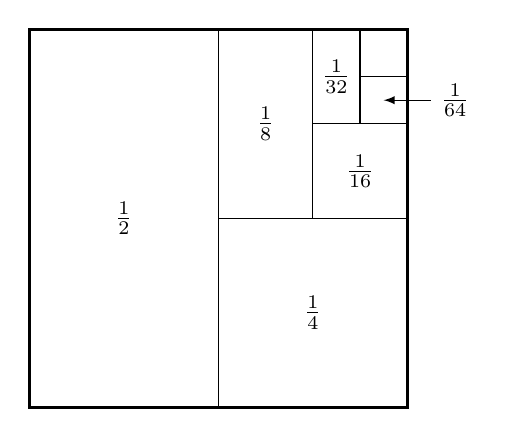
\begin{tikzpicture}[scale=.6,>=latex]
      \draw[very thick] (0,0) rectangle (8,8);
\draw(4,0)--(4,8);  \node at (2,4){$\frac{1}{2}$};
\draw (4,4)--(8,4); \node at (6,2){$\frac{1}{4}$};
\draw (6,4)--(6,8); \node at (5,6){$\frac{1}{8}$};
\draw (6,6)--(8,6); \node at (7,5){$\frac{1}{16}$};
\draw (7,6)--(7,8); \node at (6.5,7){$\frac{1}{32}$};
\draw (7,7)--(8,7); 
\draw[<-] (7.5,6.5)--(8.5,6.5)node[right] {$\frac{1}{64}$};
  \end{tikzpicture}
  \caption{}\label{fig:square}
\end{figure}
\[\frac{1}{2}+\frac{1}{4}+\frac{1}{8}+\frac{1}{16}+\frac{1}{32}+\cdots\]
从这个无穷级数里,依次取出前 $n$ 项的部分和 $S_n$, 得到数列 $\{s_n\}$:
\[s_1=\frac{1}{2},\quad s_2=\frac{1}{2}+\frac{1}{4}=\frac{3}{4},\quad s_3=\frac{1}{2}+\frac{1}{4}+\frac{1}{8}=\frac{7}{8},\ldots\]
\[s_n=\frac{1}{2}+\frac{1}{4}+\cdots+\frac{1}{2^n}=\frac{\dfrac{1}{2}\left[1-\left(\dfrac{1}{2}\right)^n\right]}{1-\dfrac{1}{2}}=1-\left(\frac{1}{2}\right)^n,\ldots\]

我们看到,这个数列 $\{s_n\}$ 和原正方形的关系是:
\begin{enumerate}
  \item 前 $n$ 项部分和 $s_n$ 小于1;
  \item $s_n$ 与 1 的误差 $|s_n-1|$, 只要 $n$ 充分大,就可以小到任意小。
\end{enumerate}
因此,前 $n$ 项部分和 $s_n$ 的极限是 1, 即
\[\lim_{n\to\infty} s_n=1 \]

我们可以这样理解无穷级数 $\sum\limits_{n=1}^{\infty}\dfrac{1}{2^n}$ 的意义,它就是前 $n$ 项部分和 $s_n$ 的极限值,于是
\[\frac{1}{2}+\frac{1}{4}+\frac{1}{8}+\cdots+\frac{1}{2^n}+\cdots=1 \]
我们说,这个无穷级数收敛到 1, 而前c$n$c项的部分和 $s_n$ 是这个极限的近似值。

现在,我们可以赋予这一类收敛的无穷级数以和的意义。

\begin{Definition}
  如果无穷级数 $u_1+u_2+\cdots+u_n+\cdots$ 的前 $n$ 项部分和 $s_n$ 所组成的数列 $\{s_n\}$ 有极限值,即 $\lim\limits_{n\to\infty}s_n=s$, 那么,这个无穷级数就叫做收敛的,并把这个确定的数 $\lim\limits_{n\to\infty}s_n=s$ 叫做这个无穷级数的和,即
\[\sum_{n=1}^{\infty}u_n=\lim_{n\to\infty}s_n=s\]
\end{Definition}
 
下面我们用收敛的数列来构造收敛的无穷级数。假设数列 $\{a_n\}$ 是收敛的,即$\lim\limits_{n\to\infty}a_n=A$, 令 $b_i=a_i-a_{i-1},\; i=1,2,\ldots$,即得一个新数列 $\{b_n\}$。无穷级数 $b_1+b_2+\cdots+b_n+b_{n+1}+\cdots$ 是收敛的。

事实上,这个级数的部分和是:
\[\begin{split}
    s_1&=b_1=a_1-a_0\\
    s_2&=b_1+b_2=(a_1-a_0)+(a_2-a_1)=a_2-a_0\\
    s_3&=b_1+b_2+b_3=(a_1-a_0)+(a_2-a_1)+(a_3-a_2)=a_3-a_0\\
    \cdots \\
    s_n&=b_1+b_2+\cdots +b_n=(a_1-a_0)+(a_2-a_1)+\cdots +(a_n-a_{n-1})=a_n-a_0\\
    \cdots \\
\end{split} \]
因此:
\begin{equation}
  \label{eq:infinity_series}
    \begin{split}
        \sum^{\infty}_{i=1}b_i&=\lim_{n\to\infty}\sum^n_{i=1}b_i=\lim_{n\to\infty}(a_n-a_0)\\
        &=\lim_{n\to\infty}a_n-a_0
    \end{split}
\end{equation}
因此,无穷级数 $\sum\limits^{\infty}_{i=1}b_i$ 是收敛的。


\begin{example}
令 $a_n=1-\dfrac{1}{n+1}$,$n=0,1,2,\ldots$,显然 $\{a_n\}$ 是收敛的,并且$\lim\limits_{n\to \infty}a_n=1$。

令\[\begin{split}
    b_i&=a_{i}-a_{i-1}=\left(1-\frac{1}{i+1}\right)-\left(1-\frac{1}{i}\right)\\
    &=\frac{1}{i}-\frac{1}{i+1}=\frac{1}{i(i+1)}
\end{split}\]
于是,      
\[\begin{split}
    \frac{1}{1\cdot 2}+\frac{1}{2\cdot 3}+\frac{1}{3\cdot 4}+\cdots +\frac{1}{n(n+1)}&=\lim_{n\to\infty}a_n-a_0\\
    &=\lim_{n\to\infty}\left(1-\frac{1}{n-1}\right)-0=1
\end{split}\]

上面\cref{eq:infinity_series} 也表示,要求一个无穷级数的和 $\sum\limits^{\infty}_{i=1}b_i$, 常将 $b_i$ 分解,使 $b_i=a_i-a_{i-1}$, 于是求无穷级数的和就转化为求数列 $\{a_n\}$ 的极限。
\end{example}

\begin{example}\label{exp:rational_series}
    求以下无穷等比级数的和。
    \[a_1+a_q+a_1q^2+\cdots +aq^{n-1}+\cdots \qquad (|q|<1)\]
\end{example}


\begin{solution}
    我们在本章中,已经证明,若 $|q|<1$,则 $\lim\limits_{n\to\infty}q^n=0$。因为:
\[s_n=\frac{a_1(1-q^n)}{1-q}=\frac{a_1}{1-q}-\frac{a_1q^n}{1-q}\]
所以,
\[\lim_{n\to\infty}s_n=\frac{a_1}{1-q}-\frac{a_1}{1-q}\lim_{n\to\infty}q^n=\frac{a_1}{1-q}\]
因此:\[a_1+a_q+a_1q^2+\cdots +aq^{n-1}+\cdots=\frac{a_1}{1-q} \quad (|q|<1)\]
\end{solution}

为了讨论循环小数及以后的需要,让我们用下面两个定理作为本节的总结。

\begin{Theorem}{定理1}
    无穷等比级数 $\sum\limits^{\infty}_{n=1}a_1q^{n-1}$ 收敛的充分必要条件是公比 $q$ 的绝对值 $|q|<1$,此时,它的和是 $\dfrac{a_1}{1-q}$,(注意这里 $q\neq 1$)。
\end{Theorem}

\begin{proof}
  上面的\cref{exp:rational_series} 已证明了 $|q|<1$ 是$\sum\limits^{\infty}_{n=1}a_1q^{n-1}=\dfrac{a_1}{1-q}$
的充分条件。要证必要性,我们只须注意到,如果 $|q|\geqslant 1$, 
那么 $a_n=a_1q^{n-1}$ 是发散的,于是,$\sum\limits^{\infty}_{n=1}a_1q^{n-1}$也是发散的(见下面的定理2)。
\end{proof}

\begin{Theorem}{定理2}
无穷级数 $\sum\limits^{\infty}_{i=1}a_i$ 收敛的必要条件是 $\lim\limits_{n\to \infty}a_n=0$.
\end{Theorem}

\begin{proof}
因为 $a_n=(a_1+a_2+\cdots +a_n)-(a_1+a_2+\cdots +a_{n-1})
=s_n-s_{n-1}$

由于 $\sum\limits^{\infty}_{i=1}a_i$ 是收敛的,故有
\[\begin{split}
    \lim_{n\to\infty}s_n&=\lim_{n\to\infty}s_{n-1}=s\\
    \lim_{n\to\infty}a_n&=\lim_{n\to\infty}(s_n-s_{n-1})=\lim_{n\to\infty}s_n-\lim_{n\to\infty}s_{n-1}=s-s=0
\end{split}\]
\end{proof}

下面的例题说明这个条件不是充分的。


\begin{example}
  $\displaystyle\frac{1}{1}+\frac{1}{2}+\frac{1}{3}+\cdots +\frac{1}{n}+\cdots$ 是发散级数,为什么呢?
\end{example}

\begin{solution}
  我们首先注意到这是正项级数,因此,部分和会越来越大,而且
\[\begin{split}
    s_1&=1          \\
    s_2&=1+\frac{1}{2}          \\
    s_4&=1+\frac{1}{2}+\frac{1}{3}+\frac{1}{4}>1+\frac{1}{2}+\frac{1}{4}+\frac{1}{4}=1+\frac{1}{2}+\frac{1}{2}          \\
    s_8&=1+\frac{1}{2}+\frac{1}{3}+\frac{1}{4}+\frac{1}{5}+\frac{1}{6}+\frac{1}{7}+\frac{1}{9}          \\
    &>1+\frac{1}{2}+\frac{1}{4}+\frac{1}{4}+\frac{1}{8}+\frac{1}{8}+\frac{1}{8}+\frac{1}{8}=1+\frac{1}{2}+\frac{1}{2}+\frac{1}{2}\\
    \cdots 
\end{split}\]

一般地,
\[s_{2^m}=1+\overbrace{\frac{1}{2}+\frac{1}{2}+\cdots +\frac{1}{2}}^{\text{$m$个}}=\frac{m+2}{2}\]    
{\linespread{1.5}\selectfont
因为,当 $m$ 无限增大时,$\dfrac{m+2}{2}$ 越来越大毫无止境,故 $s_{2^m}$ 也
发散到无穷大,又总有这样的 $n$ 满足 $2^m<n$, 故当 $m\to\infty$ 时,
也使 $m\to\infty$, $s_n>s_{2^m}\to \infty$, 即 $s_n$ 也发散到无穷大。\par}

注意到:$a_n\to 0$, 但如果数列 $\{s_n\}$中的子数列$\{s_{2^m}\}$ 是
发散的,那么 $\{s_n\}$ 也是发散的。
\end{solution}

\subsection{无限小数与十分逼近}
在这一节,我们要用无限十进小数来描述实数,要说明无限小数的意义,证明每一个循环小数都等于一个分数,而每一个分数都等于一个循环小数。

现在我们借助十分逼近法去规定实数的无限十进小数表示。考察某实数 $x$。将数轴分为单位线段,各分点均为整数。点 $x$ 在某一线段内,或者本身就是一个分点。如果 $x$ 是相邻两个单位线段的分点,约定 $x$ 属于线段的左端点。于是,存在一个整数 $\alpha_0$,使得
\[\alpha_0\le x<\alpha_0+1,\quad \text{即}\; x\in \overline{A_0B_0}=(\alpha_0,\alpha_0+1)\]

{\linespread{1.6}\selectfont$\displaystyle \alpha_0+\frac{1}{10},\; \alpha_0+\frac{2}{10},\; \alpha_0+\frac{3}{10},\;\ldots,\; \alpha_0+\frac{9}{10}$ 这些点将 $\overline{A_0B_0}=(\alpha_0,\alpha_0+1)$ 分为十等份,点 $x$ 必在某一个分段内,或者 $x$ 本身是一个分点,如果是分点,约定 $x$ 属于分段的左端
点,在这两种情况下,存在一个整数 $\alpha_1,\; (0\leqslant \alpha_1\leqslant 9)$,使得\par}
\[\alpha_0+\frac{\alpha_1}{10}\le x<\alpha_0+\frac{\alpha_1+1}{10}\]
即:$\displaystyle x\in\overline{A_1B_1}=\left[\alpha_0+\frac{\alpha_1}{10}, \alpha_0+\frac{\alpha_1+1}{10}\right)$。

\medskip
再将线段 $\overline{A_1B_1}$十等分,我们可以找到一个整数 $\alpha_2$($0\leqslant \alpha_2\leqslant 9$),使得
\[\alpha_0+\frac{\alpha_1}{10}+\frac{\alpha_2}{10^2}\le x<\alpha_0+\frac{\alpha_1+1}{10}+\frac{\alpha_2+1}{10^2}\]
即:$\displaystyle x\in\overline{A_2B_2}=\left[\alpha_0+\frac{\alpha_1}{10}+\frac{\alpha_2}{10^2}, \alpha_0+\frac{\alpha_1+1}{10}+\frac{\alpha_2+1}{10^2}\right)$。

经过 $n$ 步以后,$x$ 必在线段 $\overline{A_nB_n}$ 之中,即
\[\alpha_0+\frac{\alpha_1}{10}+\frac{\alpha_2}{10^2}+\cdots+\frac{\alpha_n}{10^n}\le x<\alpha_0+\frac{\alpha_1}{10}+\frac{\alpha_2}{10^2}+\cdots+\frac{\alpha_n+1}{10^n}\]
这里 $\alpha_1,\alpha_2,\ldots,\alpha_n$ 都是 0 到 9 之间的整数,线段$\overline{A_nB_n}$ 之长度等于 $\dfrac{1}{10^n}$,而有限十进小数$\alpha_0.\alpha_1\alpha_2\cdots\alpha_n$ 和 $\alpha_0.\alpha_1\alpha_2\cdots(\alpha_n+1)$ 分别是 $x$ 的准确到 $\dfrac{1}{10^n}$ 的不足近似值和过剩近似值。

让这个十分逼近过程无限地进行下去,那么实数 $x$ 就完全可以由无限小数$\alpha_0.\alpha_1\alpha_2\cdots\alpha_n\cdots$ 来表示,同时由于 $x$ 与有限
小数近似值的误差
\[|\alpha_0.\alpha_1\alpha_2\cdots\alpha_n-x|<\frac{1}{10^n},\qquad  |\alpha_0.\alpha_1\alpha_2\cdots(\alpha_n+1)-x|<\frac{1}{10^n}\]
当 $n$ 充分大时,可以小到任意小,所以无限小数 $x=\alpha_0.\alpha_1\alpha_2\cdots\alpha_n\cdots$ 是由有限十进小数组成的两个数列:
\[\alpha_0,\; \alpha_0.\alpha_1,\;\alpha_0.\alpha_1\alpha_2,\;\ldots,\;  \alpha_0.\alpha_1\alpha_2\cdots\alpha_n,\;\ldots\]
与
\[(\alpha_0+1),\; \alpha_0.(\alpha_1+1),\;\alpha_0.\alpha_1(\alpha_2+1),\;\ldots, \alpha_0.\alpha_1\alpha_2\cdots(\alpha_n+1),\;\ldots\]
的共同的极限值。

\emph{无限小数的定义}是这样的,我们取实数的小数点以下第 $n$ 位为止的有限小数 $\alpha_0.\alpha_1\alpha_2\cdots\alpha_n$,记作 $x_n$,即 $x_n=\alpha_0.\alpha_1\alpha_2\cdots\alpha_n$,那么数列 $\{x_n\}$ 的极限值是这个无限小数,用式子表示就是
\[\lim_{n\to\infty}x_n=x=\alpha_0.\alpha_1\alpha_2\cdots\alpha_n\cdots\]


\begin{example}
$\dfrac{2}{3}=0.\dot{6}$表示数列$\{x_n\}$的极限:
\[x_1=0.6,\; x_2=0.66,\; x_3=0.666,\ldots,\; x_n=0.\underbrace{66\cdots 66}_{\text{$n$位小数}},\; \ldots\]
\end{example}

\begin{example}
  无限小数 $\uppi=3.1415926\cdots$ 的意思是,令
  \[ x_1=3.1,\; x_2=3.14,\; x_3=3.141,\; \ldots\]
  那么 $x_n\to \uppi$。
\end{example}

注意,在上面我们用十分逼近得到实数 $x$ 的无限十进小数表示时,在 $x$ 是十等分的一个分点的情形,如果不限定 $x$ 属于两相邻线段的左端点,那么对于同一个整数或有限小数,可能有两类不同的无限十进小数表示法。例如
\[1=1.0000\cdots=0.999\cdots,\quad 2.35=2.35000\cdots=2.34999\cdots\]

为排除这种不确定性,按照我们的约定,就可以去掉那些从某一位以后有数字都是 9 的十进小数表达式。

把实数写成小数形式,便于比较它们的大小。在比较时,遇到以 9 为循环节结尾的无限小数都用以 0 为循环节结尾的无限小数代替。

今有两个实数 $x=\alpha_0.\alpha_1\alpha_2\cdots\alpha_n\cdots$ 和 $y=\beta_0.\beta_1\beta_2\cdots\beta_n\cdots$,比较这两个实数 $x$ 和 $y$ 的大小,只须比较两个数的各数位上的数字,并且注意在哪一个数位上的数字不同,从而告诉我
们哪个实数大。


{\linespread{1.6}\selectfont 例如:$\dfrac{17}{20}=0.850000\cdots$,$\dfrac{45}{53}=0.84905000\cdots$,看一眼就能发觉,它们有相同的第一位小数,$\frac{17}{20}$ 的第二位小数大于 $\frac{45}{53}$ 的第二位小数,因此,$\dfrac{17}{20}>\dfrac{45}{53}$。\par}

\medskip
一般地,我们说 $x>y$,如果下面的条件中有一个成立
\begin{enumerate}
  \item $\alpha>\beta$
  \item $\alpha=\beta$,而 $\alpha_1>\beta_1$
  \item $\alpha=\beta, \alpha_1 =\beta_1,\ldots,\alpha_{\ell}=\beta_{\ell}$,而 $\alpha_{\ell+1}>\beta_{\ell+1}$
\end{enumerate}

\bigskip
根据前面的讨论,我们知道任何一个实数都是两个有限十进小数的夹逼数列的极限。

设 $\lim x_n=x=\lim x'_n,\quad \lim y_n=y=\lim y'_n$,或者
\[x_n\to x\leftarrow x'_n,\qquad y_n\to y\leftarrow y'_n\]
\[x'_n-x_n\to 0,\qquad y'_n-y_n\to 0\]
则对应数列的相加,我们有实数的相加,对应于数列相乘,我们有实数的相乘,也就是说:
\[\begin{split}
  \lim(x_n+y_n)&=x+y=\lim(x'_n+y'_n)\\
  \lim(x_n\cdot y_n)&=x\cdot y=\lim(x'_n\cdot y'_n)
\end{split}
\]

例如 $\sqrt{2}=1.4142135\cdots,\quad \sqrt{3}=1.7320508\cdots$,
\[\begin{cases}
    x_n+y_n\\  x'_n+y'_n
\end{cases}\qquad \begin{cases}
    1.4+1.7=3.1 \\ 1.5+1.8=3.3
\end{cases}\]
\[\begin{cases}
    1.41+1.73=3.14\\1.42+1.74=3.16
\end{cases}\qquad \begin{cases}
    1.414+1.732=3.146\\1.415+1.733=3.148
\end{cases}\]
\[\begin{cases}
    1.4142+1.7320=3.1462\\
1.4143+1.7321=3.1464
\end{cases}\qquad \begin{cases}
    1.41421+1.73205=3.14626\\
1.41422+1.73206=3.14628
\end{cases}\cdots\]
即:
$3.1 <3.14<3.146<3.1462<3.14626<\cdots <\sqrt{2}+\sqrt{3}<\cdots <3.14628<3.1464<3.148<3.16<3.3$

$\therefore\quad \sqrt{2}+\sqrt{3}=3.1462\cdots$。只要把 $\sqrt{2}$, $\sqrt{3}$ 的夹逼小数求到足够多的数位,我们用上面的方法就可以把 $\sqrt{2}+\sqrt{3}$ 的小数表示求到任意的数位上。

同样地得到
\[\begin{cases}
    x_n\cdot y_n\\  x'_n\cdot y'_n
\end{cases}\qquad \begin{cases}
    1.4\times 1.7=2.38 \\ 1.5\times 1.8=2.70
\end{cases}\qquad \begin{cases}
    1.41\times 1.73=2.4393\\1.42\times 1.74=2.4708
\end{cases}\]
\[\begin{cases}
    1.414\times 1.732=2.449048\\1.415\times 1.733=2.452195
\end{cases}\qquad \begin{cases}
    1.4142\times 1.7320=2.4493944\\
1.4143\times 1.7321=2.449709
\end{cases}\cdots\]

$\therefore\quad \sqrt{6}=2.449\cdots$。

在无限小数中,除了有一类\emph{无限循环小数},还有一类\emph{无限不循环小数},譬如,$0.1001000100001\cdots$,就是一个无限不循环小数。

现在我们要来证明每一个循环小数都等于一个分数,而每一个分数都等于一个循环小数。先举几个将无限循环小数化为分数的例子,再给出一般的证明。

\begin{example}
  怎样将循环小数 $0.\overline{621}$ 化成分数?
\end{example}

\begin{solution}
  我们可以将无限小数 $0.\overline{621}$ 表示成一个无穷级数
\[\begin{split}
0.\overline{621}&=0.621+0.000621+0.000000621+\cdots\\
&=\frac{621}{10^3}+\frac{621}{10^6}+\frac{621}{10^9}+\cdots
\end{split}\]
显然,这个无穷级数是无穷等比级数,它的首项 $a_1=\dfrac{621}{10^3}$, 公比$q=\dfrac{1}{10^3}$ 根据 4.1 中的定理,这个无穷等比级数的和是 $\dfrac{a_1}{1-q}$,因此:
\[\begin{split}
    0.\overline{621}&=\frac{621}{10^3}+\frac{621}{10^6}+\frac{621}{10^9}+\cdots\\
    &=\frac{621}{10^3}\cdot \frac{1}{1-\frac{1}{10^3}}=\frac{621}{10^3}\cdot \frac{10^3}{10^3-1}\\
    &=\frac{621}{999}=\frac{23}{37}
\end{split}\]
\end{solution}

\begin{example}
试将$0.3\overline{12}$化成分数。
\end{example}

\begin{solution}
\[\begin{split}
    0.3\overline{12}&= 0.3+0.0\overline{12}=0.3+(0.012+0.00012+\cdots)\\
    &=\frac{3}{10}+\left(\frac{12}{10^3}+\frac{12}{10^5}+\cdots\right)\\
    &=\frac{3}{10}+\frac{12}{10^3}\cdot \frac{1}{1-\dfrac{1}{10^2}}\\
    &=\frac{3}{10}+\frac{12}{10^3}\cdot \frac{10^2}{10^2-1}\\
    &=\frac{3}{10}+\frac{12}{10}\cdot \frac{1}{99}=\frac{309}{990}=\frac{103}{330}
\end{split}\]
\end{solution}

下面,我们来证明任何一个循环小数一定是一个分数。

如果 $a$ 是个循环小数,它的循环节是由第 $k+1$ 位开始到 $k+\ell$ 位,平常我们写作
\[a=a_0.c_1c_2\cdots c_k\overline{c_{k+1}c_{k+2}\cdots c_{k+\ell}}\]
它的意思是
\[\begin{split}
    a&=a_0+\frac{c_1}{10}+\frac{c_2}{10^2}+\cdots +\frac{c_k}{10^k}+\frac{c_{k+1}}{10^{k+1}}+\cdots+\frac{c_{k+\ell}}{10^{k+\ell}}\\
&\qquad +\frac{c_{k+1}}{10^{k+\ell+1}}+\cdots+\frac{c_{k+\ell}}{10^{k+2\ell}}+\frac{c_{k+1}}{10^{k+2\ell+1}}+\cdots+\frac{c_{k+\ell}}{10^{k+3\ell}}+\cdots
\end{split}\]

虽然,这不是无穷等比级数,现在用结合律来构造这个无穷级数的部分和的子数列:

设 $S_1=a_0+\dfrac{c_1}{10},\quad S_2=a_0+\dfrac{c_1}{10}+\dfrac{c_2}{10^2},\ldots$ 于是第 $k$ 个部分和是
\[S_k=a_0+\frac{c_1}{10}+\frac{c_2}{10^2}+\cdots+\frac{c_k}{10^k}\]
再令
\[d=\frac{c_{k+1}}{10^{k+1}}+\frac{c_{k+2}}{10^{k+2}}+\cdots +\frac{c_{k+\ell}}{10^{k+\ell}}\]
所以,$d$ 是分数,而且 $0\leqslant d<1$。

那么,第 $k+m\ell$ 个部分和是
\[\begin{split}
    S_{k+m\ell}&=S_k+d+\frac{d}{10^{\ell}}+\frac{d}{10^{2\ell}}+\cdots \frac{d}{10^{(m-1)\ell}}\\
    &=S_k+d\left(1+\frac{1}{10^{\ell}}+\frac{1}{10^{2\ell}}+\cdots +\frac{1}{10^{(m-1)\ell}}\right)\\
    &=S_k+\frac{d\left(1-\dfrac{1}{10^{m\ell}}\right)}{1-\dfrac{1}{10^{\ell}}}
\end{split}\]
当 $m=1,2,3,\ldots$ 时,部分和 $S_{k+m\ell}$ 就构成无穷级数的部分和数列 $\{S_n\}$ 的子数列 $\{S_{k+m\ell}\}$, 并且
\[\begin{split}
    \lim_{m\to\infty}S_{k+m\ell}&= \lim_{m\to\infty}\left\{S_k+\frac{d\left(1-\frac{1}{10^{m\ell}}\right)}{1-\frac{1}{10^{\ell}}}\right\}\\
    &=S_k+\frac{d}{1-\frac{1}{10^{\ell}}}=S_k+\frac{10^{\ell}\cdot d}{10^{\ell}-1}=a'
\end{split}\]
这里 $a'$ 表示分数。我们只证明了部分和数列的子数列 $\{S_{k+m\ell}\}$ 收敛到分数
$a'$,还需要证明部分和数列 $\{S_n\}$ 也收敛到 $a'$。

我们只须注意到原来的循环小数所代表的无穷级数也都是正项的,这就是说,部分和数列$\{S_n\}$是递增数列,特别地,如果 $k+m\ell\leqslant n<k+(m+1)\ell$,
那么 $S_{k+m\ell}\leqslant S_n\leqslant S_{k+(m+1)\ell}$,因此,如果“子数列” $\{S_{k+m\ell},\; m=1,2,3,\ldots\}$ 收敛到 $a'$, 原数列 $\{S_n\}$也收敛到 $a'$。

我们已证明了,每个循环小数都可以化为分数,现在证明分数可以化为循环小数。

设 $\dfrac{a}{b}$ 为一任意给定的不可约真分数(亦即 $a,b$ 互质且 $a<b$)。

\medskip
\begin{enumerate}
  \item $b$ 只含有 2 或 5 的质因子,则容易看出可以化 $\dfrac{a}{b}$ 成有限位小数。

事实上,设 $b=2^{\alpha}5^{\beta}$, $d=5^{\alpha-\beta}a$,若 $\alpha\geqslant \beta$,则
\[\frac{a}{b}=\frac{a}{2^{\alpha}5^{\beta}}=\frac{5^{\alpha-\beta}a}{10^{\alpha}}=\frac{d}{10^{\alpha}}\]
为 $\alpha$ 位小数。我们可以把有限位小数看成循环小数的特例。如:
\[\frac{1237}{2\times 5^3}=\frac{1237\times 2^2}{10^3}=4.948=4.948\overline{0}\]

\item\label{itm:proof_fraction_step2} 设 $b$ 与 10 互质,即:$(b,10)=1$, 根据整数分解的唯一性而知 $\dfrac{a}{b}$ 不可能写成 $\dfrac{m}{10^k}$ 的形式,这里 $m$ 为正整数,故 $\dfrac{a}{b}$ 不可能化为有限小数。做除法,我们得到
\[10a=bq_1+r_1,\qquad 0<r_1<b\]
两边再除以 $b$,得
\[\frac{10a}{b}=q_1+\frac{r_1}{b},\qquad 0<\frac{r_1}{b}<1\]

这里 $q$ 是 $0,1,2,\ldots,9$ 这十个整数中的某个。用和上面同样的方法,逐步得到
\[\begin{split}
    \frac{10r_1}{b}&=q_2+\frac{r_2}{b},\qquad 0<\frac{r_2}{b}<1,\\
    \frac{10r_2}{b}&=q_3+\frac{r_3}{b},\qquad 0<\frac{r_3}{b}<1,\\
\cdots  \\
    \frac{10r_{n-1}}{b}&=q_n+\frac{r_n}{b},\qquad 0<\frac{r_n}{b}<1\\
\end{split}\]
这里每个 $q_n$ 是 $0,1,2,\ldots,9$ 这十个整数中的某个,于是
\[\begin{split}
    \frac{a}{b}&=\frac{q_1}{10}+\frac{r_1}{10b}\\
    &=\frac{q_1}{10}+\frac{q_2}{10^2}+\frac{r_2}{10^2b}\\
    &=\frac{q_1}{10}+\frac{q_2}{10^2}+\frac{q_3}{10^3}+\frac{r_3}{10^3b}\\
    \cdots  \\
    &=\frac{q_1}{10}+\frac{q_2}{10^2}+\cdots+\frac{q_n}{10^n}+\frac{r_n}{10^n b}\\
\end{split}\]

再设
\[\begin{split}
    x_n&=\frac{q_1}{10}+\frac{q_2}{10^2}+\cdots+\frac{q_n}{10^n}\\
    y_n&=\frac{q_1}{10}+\frac{q_2}{10^2}+\cdots+\frac{q_n+1}{10^n}\\
    d_n&=\frac{r_n}{10^n b}<\frac{1}{10^n}
\end{split}\]
则:
\[\frac{a}{b}=x_n+d_n,\qquad 0<d_n<\frac{1}{10^n}\]

再有 $x_1<x_2<\cdots<x_{n-1}<x_n<\cdots<y_n<y_{n-1}<\cdots<y_2<y_1$,且 $y_n-x_n\to 0$。

当 $n$ 无限增大时,根据实数完备性,无限小数
\[\sum_{n=1}^{\infty}\frac{q_n}{10^n}=0.q_1q_2\cdots q_n\cdots\]
为一实数,又因为 $d_n\to 0$,故我们确定了一个其值为 $\dfrac{a}{b}$ 的无限小数 $0.q_1q_2\cdots q_n\cdots$。

\medskip
{\linespread{1.4}\selectfont
再说明这个无限小数一定是纯循环小数,设 $a=r_0$, 因为
$r_0,r_1,r_2,\ldots,r_n,\ldots$ 是一串大于 0 而小于 $b$ 的正整数,这种正整数只有 $b-1$ 个不同的,所以,这一串数 $r_0=a,r_1,r_2,\ldots r_n,\ldots$ 必然有二者会相同,就假定 $r_k$ 为首先出现的重见余数,假定这两个相同的余数是 $r_k$ 和 $r_i$, 即有 $r_k=r_i$。现在我们要证明 $r_i$ 只能是 $a=r_0$,用反证法,若 $i>0$ 则由等式
$\dfrac{10r_{k-1}}{b}=q_k+r_k$ 和 $\dfrac{10r_{i-1}}{b}=q_i+r_i$ 两边作减法,得到\par}
\[\frac{10(r_{k-1}-r_{i-1})}{b}=q_k-q_i\]
因为 $q_k-q_i$ 是整数,所以 $b$ 能整除 $10(r_{k-1}-r_{i-1})$,由于 $b$ 与 10
互质,故 $b$ 能整除 $r_{k-1}-r_{i-1}$,但是 $r_{k-1}-r_{i-1}<b$,所以 $r_{k-1}-r_{i-1}=0$,即 $r_{k-1}=r_{i-1}$ 重见更早,与原设 $r_k$ 为首先出现的重见余数不合,故 $i=0$。

$\therefore\quad r_k=r_0=a$, 这样
\[\frac{a}{b}=0.\overline{q_1q_2\cdots q_{k-1}q_k}\]

\item 设 $b=2^{\alpha}5^{\beta}b_1$, 而 $b_1>1$ 且与 10 互质,又 $\alpha$ 与 $\beta$ 均不为 0, 若 $\alpha\geqslant \beta$,
\[\frac{a}{b}=\frac{a}{2^{\alpha}5^{\beta}b_1}=\frac{5^{\alpha-\beta}a}{10^{\alpha}b_1}\]
做 $5^{\alpha-\beta}a$ 除以 $b_1$,得
\[5^{\alpha-\beta}a=M{b_1}+{r},\quad 0<r<b\]
$M$ 是一个正整数,两边再除以 $b_1$,得
\[5^{\alpha-\beta}\frac{a}{b_1}=M+\frac{r}{b_1},\qquad 0<\frac{r}{b_1}<1\]
由前段证明 \ref{itm:proof_fraction_step2} 的结果
\[\frac{r}{b_1}=0.\overline{c_1c_2\cdots c_{s}}\]
故,
\[\begin{split}
    \frac{a}{b}&=\frac{5^{\alpha-\beta}a}{10^{\alpha}b_1}=\frac{1}{10^{\alpha}}\left(M+0.\overline{c_1c_2\cdots c_{s}}\right)\\
    &=\frac{1}{10^{\alpha}}\left(M.\overline{c_1c_2\cdots c_{s}}\right)
\end{split}\]

当以 $10^{\alpha}$ 除以 $M.\overline{c_1c_2\cdots c_{s}}$ 时,也就是将小数点左移$\alpha$ 位,我们得到
\[\frac{a}{b}=0.m_1m_2\cdots m_{\alpha}\overline{c_1c_2\cdots c_{s}}\]
为混循环小数。
\end{enumerate}

若 $\alpha\le \beta$,可以用同样的方法说明 $\dfrac{a}{b}$ 为一混循环小数,因
此有
\begin{Theorem}{定理}
    任何一个分数都等于某一个循环小数,任何一个循环小数必然是个分数。
\end{Theorem}

如果采用无限十进小数来描述实数,我们按照下表来对实数分类:
\[\text{实数——无限十进小数}\begin{cases}
    \text{有理数—无限十进循环小数}\\
    \text{无理数—无限十进不循环小数}
\end{cases}\]

\begin{Exercise}
\begin{question}
    \item 求下列无穷等比数列的和:
  \begin{tasks}(2)
    \task $\displaystyle \frac{1}{2}+\frac{1}{3}+\frac{2}{9}+\cdots$
    \task $\displaystyle 1-\frac{2}{5}+\frac{4}{25}-\cdots$
    \task $\displaystyle \sqrt{\frac{3}{2}}+\sqrt{\frac{2}{3}}+\frac{2}{3}\sqrt{\frac{2}{3}}+\cdots$
    \task $\displaystyle \frac{\sqrt{3}+1}{\sqrt{3}-1}+1+\frac{\sqrt{3}-1}{\sqrt{3}+1}+\cdots$
  \end{tasks}        
  \item 若 $a,b$ 是实数且 $\left|\dfrac{a+2b+3}{b+3}\right|+3(a+3b)^2=0$, 求等比级数 $ab+b+\dfrac{b}{a}+\cdots$ 的和。
  \item 已知 $\sqrt{3}\sin\alpha-\cos\alpha=0$, $\alpha$ 为锐角,求 $\sum\limits^{\infty}_{n=0}(-\sin\alpha)^n$
  \item 求下列无穷级数的和:
  \begin{tasks}
    \task $\displaystyle \frac{1}{1 \times 4}+\frac{1}{2 \times 5}+\frac{1}{3 \times 6}+\frac{1}{4 \times 7}+\cdots$
    \task $\displaystyle \frac{6}{2 \times 7}+\frac{6}{7 \times 12}+\frac{6}{12 \times 17}+\frac{6}{17 \times 22}+\cdots$
    \task $\displaystyle \frac{1}{1 \times 2 \times 3}+\frac{1}{2 \times 3 \times 4}+\frac{1}{3 \times 4 \times 5}+\frac{1}{4 \times 5 \times 6}+\cdots$
    \task $\displaystyle \frac{1}{1 \times 2 \times 3 \times 4}+\frac{1}{2 \times 3 \times 4 \times 5}+\frac{1}{3 \times 4 \times 5 \times 6}+\frac{1}{4 \times 5 \times 6 \times 7}+\cdots$
    \task $\displaystyle \frac{1}{7}+\frac{2}{7^{2}}+\frac{3}{7^{3}}+\frac{1}{7^{4}}+\frac{2}{7^{6}}+\frac{3}{7^{6}}+\frac{1}{7^{7}}+\frac{2}{7^{8}}+\frac{3}{7^{9}}+\cdots$
  \end{tasks}
  \item 求下列各式的极限值:
  \begin{tasks}
      \task $\displaystyle \lim _{n\to  \infty} \frac{1+a+a^{2}+\cdots+a^{n}}{1+b+b^{2}+\cdots+b^{n}} \qquad(|a|<1,\;|b|<1)$
      \task $\displaystyle \lim _{n\to  \infty}\left(\frac{1}{n}-\frac{2}{n}+\frac{3}{n}-\cdots+\frac{(-1)^{n-1} n}{n}\right)$
      \task $\displaystyle \lim _{n\to  \infty}\left(\frac{1^{2}}{n^{3}}+\frac{2^{2}}{n^{3}}+\cdots+\frac{(n-1)^{2}}{n^{3}}\right)$
      \task $\displaystyle \lim _{n\to  \infty}\left(\frac{1}{2}+\frac{3}{{2^2}}+\frac{5}{2^3}+\cdots+\frac{2n-1}{2^{n}}\right)$
  \end{tasks}
  \item $\displaystyle \lim_{n\to  \infty}\left(1-\frac{1}{2^2}\right)\left(1-\frac{1}{3^2}\right)\left(1-\frac{1}{4^2}\right)\cdots\left(1-\frac{1}{n^2}\right)$
  \item 数列 $x_n\; (n=1,2,3,\ldots)$ 是由下列各式所确定:
\[x_0=a,\; x_1=b,\; x_n=\frac{x_{n-2}+x_{n-1}}{2}\quad (n\ge 2)\]
求 $\lim\limits_{n\to\infty}x_n$.
  \item 将下列循环小数化为分数:
  \[0.\overline{47},\qquad 2.\overline{234},\qquad 0.4\overline{7},\qquad 3.2\overline{31},\qquad 0.\overline{1108},\qquad 5.38\overline{90}\]
  \item 求出下列各式的值:
  \begin{tasks}(2)
    \task $0.\overline{48}\times0.\overline{48}$
    \task $0.\overline{12}+0.\overline{83}+0.\overline{34}+\cdots+0.\overline{89}$
    \task $0.\overline{15}+0.0\overline{15}+0.00\overline{15}+\cdots$
  \end{tasks}
\end{question}
\end{Exercise}

\section{数列极限在几何上的应用}
在平面几何中,我们知道了什么是相似形,而且知道研究相似形的基本定理是“设 $\triangle ABC$ 和 $\triangle A'B'C'$ 的三个内角对应相等,则其对应边长成比例”。在初中时,我们证明了当比值是有理数时,定理是对的,现在要补充推证,在比值是无理数时,定理也是对的,这样这个定理的证明才是完整的。

\begin{proof}
设 $AB=kA'B'$, 这里 $k$ 是无理数,我们要证明
\[\frac{AC}{A'C'}=\frac{BC}{B'C'}=k\]
我们知道任何一个无理数可以用有理数来逼近,于是可以找到两串有理数 $k'_n,k''_n$ 从左、右夹逼无理数 $k$ 使得
\[k'_n\to k\leftarrow k''_n,\quad \text{或者}\quad \lim_{n\to\infty}k'_n=\lim_{n\to\infty}k''_n=k\]
比如,$k$ 是特殊的情形,$k=\sqrt{2}$,则可取
\[\begin{split}
    k'_1&=1,\quad     k'_2=1.4,\quad    k'_3=1.41,\;\ldots\\ 
    k''_1&=1,\quad     k''_2=1.5,\quad    k''_3=1.42,\;\ldots\\
\end{split}\]

\begin{figure}
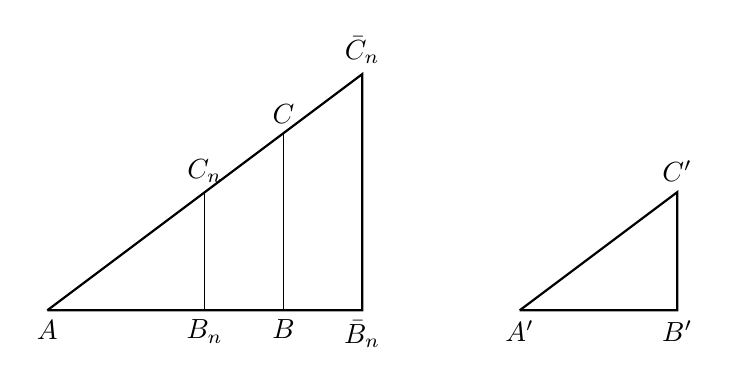
\begin{tikzpicture}
\begin{scope}
  \draw[thick] (0,0)node[below]{$A$}--(4,0)node[below]{$\bar{B}_n$}--(4,3)node[above]{$\bar{C}_n$}--(0,0);
  \draw(3,0)node[below]{${B}$}--(3,2.25)node[above]{$C$};
  \draw(2,0)node[below]{${B}_n$}--(2,1.5)node[above]{${C}_n$};
\end{scope}
\begin{scope}[xshift=6cm]
\draw[thick] (0,0)node[below]{$A'$}--(2,0)node[below]{$B'$}--(2,1.5)node[above]{$C'$}--(0,0);
\end{scope}
\end{tikzpicture}
    \caption{}\label{fig:sim_ratio}
\end{figure}

如\cref{fig:sim_ratio},在直线 $AB$ 上取点列 $\{B_n\}$和$\{\bar{B}_n\}$ 使得
\[AB_n=k'_nA'B',\qquad A\bar{B}_n=k''_n A'B'\]
再由 $B_n$, $\bar{B}_n$点 分别作 $BC$ 边平行线交 $AC$ 线于 $C_n$,$\bar{C}_n$点,则因为相似三角形定理对有理数比值是对的,所以
\[\triangle AB_nC_n \sim \triangle A\bar{B}_n\bar{C}_n \sim \triangle A'B'C'\]
\[\begin{split}
  \frac{AB_n}{A'B'}&=\frac{AC_n}{A'C'}=\frac{B_nC_n}{B'C'}=k'_n\\
  \frac{A\bar{B}_n}{A'B'}&=\frac{A\bar{C}_n}{A'C'}=\frac{\bar{B}_n\bar{C}_n}{B'C'}=k''_n\\
\end{split}\]
由作图知
\[k'_nA'B'=AB_n<AB<A\bar{B}_n=k''_nA'B'\]
并可得
\[\begin{split}
     k'_nA'C'&=AC_n<AC<A\bar{C}_n=k''_nA'C'\\
k'_nB'C'&=B_nC_n<BC<\bar{B}_n\bar{C}_n=k''_nB'C'
\end{split}\]
对上面不等式各端取极限,得到
\[\lim_{n\to\infty} k'_n A'C'  =  \lim_{n\to\infty}k''_n A'C'   =kA'C'\]
另一方面又可得到
\[\lim_{n\to\infty} k'_n A'C' = \lim_{n\to\infty}k''_n A'C'  =AC\]
根据数列的极限值是唯一的,因此 $AC=kA'C'$,同理可得
$BC=kB'C'$。
\end{proof}

\bigskip
总结上面的证明可以归纳成下面两点:
\begin{enumerate}
  \item 先有一个数 $k$, 因为它是无理数,比较复杂,往往我们要用简单的有理数逐步逼近它;
  \item 在求极限过程中,要点是要用极限值的唯一性保证所要的结论。
\end{enumerate}

\medskip
在几何上,$\uppi$ 表示单位圆的面积,这个面积 显然能用一个有理数或无理数来表示,可是,如果我们想要以任何精确度计算出数元,这个定义对于我们来说并没有什么帮助。这
时,我们必须借助于求极限的过程,把数 $\uppi$ 表示为已知并且不难算出的数列的极限,除此外别无它法。

假如我们把单位圆等分成 $2n$ 个小扇形,然后一上一下间插排列起来,如\cref{fig:divide_circle}。
\begin{figure}
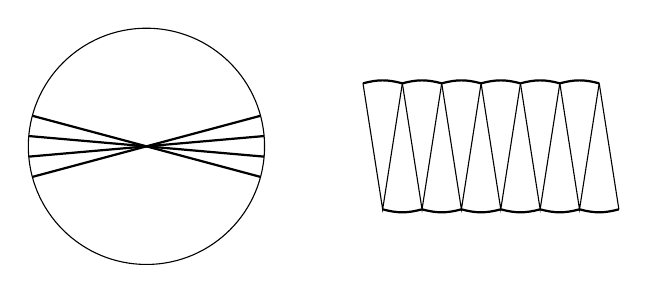
\begin{tikzpicture}
\begin{scope}
    \draw (0,0) circle (1.5);
    \foreach \x in {15,-5,5,-15}
    {
        \draw[thick] (\x:1.5)--(\x+180:1.5);
    }
\end{scope}
\begin{scope}[xshift=3cm]
    \foreach \x in {0,.5,1,...,2.5}
    {
        \draw[thick] (\x,-.8) to[bend right=15] (\x+.5,-.8);
        \draw[thick] (\x-.25,.8) to[bend right=-15] (\x+.25,.8);
        \draw[smooth] (\x+.25,.8)--(\x,-.8)--(\x-.25,.8) ;
    }
    \draw[smooth] (3,-.8)--(3-.25,.8) ;
\end{scope}
\end{tikzpicture}
    \caption{}\label{fig:divide_circle}
\end{figure}

当 $n$ 愈大时,上图就愈接近一个高为 1, 面积为 $\uppi$ 的矩形。这也就说明了单位圆的圆周长等于 $2\uppi$。

早在三国时代,我国古代数学家刘徽于公元 263 年在《九章算术》中,对古率 $\uppi=3$ 极为不满,就提出了用折线逐步地来逼近曲线,用正多边形的面积来逐步地逼近圆的面积的思想,他说如果圆内接正六边形,正十二边形,二十四边形……依次递求它的面积,边数愈增多则其面积与圆面积 愈加接近,如果边数增加到无限则多边形面积的极限就与圆面积相等。

设 $\uppi$ 为单位圆面积,$S_n$ 为单位圆的内接正 $n$ 边形的面积,$S$ 为单位圆的外切正 $n$ 边形的面积,如\cref{fig:polygon_circle},对于每一个 $n$,从几何直观上作如下估计
\begin{figure}
\begin{tikzpicture}[>=latex, scale=1.8]
\draw (0,0) circle (1);
\draw[thick] (30:1)--(90:1)--(150:1)--(210:1)--(270:1)--(330:1)--(30:1);
\draw [thick](0:1.165)--(60:1.165)--(120:1.165)--(180:1.165)--(240:1.165)--(300:1.165)--(0:1.165);
\draw (0,0)node[left]{$O$}--(0:1.165);
\draw  (-30:1)--(0,0)-- (30:1);
\draw[|<->|] (1.8,0) --node[right]{$\sin\dfrac{\uppi}{n}$}(1.8,.5);
\draw (.25,0) arc (0:30:.25)node[right]{$\uppi/n$}; 
\draw[|<->|] (1.26,0) --node[right]{$\tan\dfrac{\uppi}{n}$}(30:1.1);
\node at (42:.5){1};
\end{tikzpicture}   
    \caption{}\label{fig:polygon_circle}
\end{figure}

$S_n<S_{2n}<\uppi<S'_{2n}<S'_n$, 
刘徽的计算理论基础是,$|S_n-\uppi|<S'_n-S_n$, 在 $n$ 无限增大时,$(S'_n-S_n)\to 0$。从\cref{fig:polygon_circle} 看出:
\[\begin{split}
    S'_n&=2n\text{直角三角形的面积}=2n\cdot \frac{1}{2}\tan\frac{\uppi}{n}=n\tan\frac{\uppi}{n}   \\
    S_n&=2n\text{直角三角形的面积}=2n\cdot \frac{1}{2}\cos\frac{\uppi}{n}\cdot \sin \frac{\uppi}{n}=n\sin\frac{\uppi}{n}\cdot \cos\frac{\uppi}{n}
\end{split}\]

\[\begin{split}
    S'_n-S_n &= n\left(\tan\frac{\uppi}{n}-\sin\frac{\uppi}{n}\cdot \cos\frac{\uppi}{n}\right)\\
    &=n \sin\frac{\uppi}{n}\left(\frac{1}{\cos\dfrac{\uppi}{n}}-\cos\frac{\uppi}{n}\right)\\
    &=\frac{1}{2}(\text{圆内接 $n$ 边形周长})\left(\frac{1}{\cos\dfrac{\uppi}{n}}-\cos\frac{\uppi}{n}\right)\\
    &<\frac{1}{2}(\text{圆外切六边形周长})\left(\frac{1}{\cos\dfrac{\uppi}{n}}-\cos\frac{\uppi}{n}\right)\to 0\\
\end{split} \]

这就说明了由圆内接正多边形的面积所组成的数列 $\{S_{6\cdot 2^{n-1}}\}$ 的极限是 $\uppi$. 

让我们计算这个数列中的前面几个面积。面积的通项是
\[S_{6\cdot 2^{n-1}}=6\cdot 2^{n-1}\left(\frac{1}{2}\sin\frac{\uppi}{3\cdot 2^{n-1}}\right)=3\cdot 2^{n-1}\sin\frac{\uppi}{3\cdot 2^{n-1}}\quad (n=1,2,3,\ldots)\]

为由 $\sin\dfrac{\uppi}{n}$ 求出 $\sin\dfrac{\uppi}{2n}$,我们需要导出它们之间的递推关系:
\[\begin{split}
    \sin\frac{\uppi}{2n}&=\sqrt{\frac{1-\cos\dfrac{\uppi}{n}}{2}}\\
    &=\frac{1}{2}\sqrt{2-2\cos\frac{\uppi}{n}}\\
    &=\frac{1}{2}\sqrt{2-2\sqrt{1-\sin^2\frac{\uppi}{n}}}
\end{split}\]
于是:
\begin{itemize}[itemsep=5pt]
    \item 当 $n=1$, $S_6=3\cdot \sin \dfrac{\uppi}{3}=2.5980762$, 
    \item 当 $n=2$, $S_{12}=6\cdot \sin \dfrac{\uppi}{6}=3$,
    \item 当 $n=3$, 
    \[\begin{split}
        S_{24}&=12\cdot \sin \frac{\uppi}{12}=12\left(\frac{1}{2}\sqrt{2-2\sqrt{1-\left(\frac{1}{2}\right)^2}}\right)\\
        &=12\cdot \left(\frac{1}{2}\sqrt{2-\sqrt{3}}\right)=12\times 0.258819=3.1058285
    \end{split}\]
    \item 当 $n=4$, 
    \[\begin{split}
        S_{48}&=24\cdot \sin \frac{\uppi}{24}=24\left(\frac{1}{2}\sqrt{2-2\sqrt{1-0.258819^2}}\right)\\
        &=24\times 0.1305266=3.132639
    \end{split}\]
    \item 当 $n=5$, 
    \[\begin{split}
        S_{96}&=48\cdot \sin \frac{\uppi}{48}=48\left(\frac{1}{2}\sqrt{2-2\sqrt{1-0.1305266^2}}\right)\\
        &=48\times 0.0654031=3.1393515
    \end{split}\]
    \item 当 $n=6$, 
    \[\begin{split}
        S_{192}&=96\cdot \sin \frac{\uppi}{96}=96\left(\frac{1}{2}\sqrt{2-2\sqrt{1-0.0654031^2}}\right)\\
        &=96\times 0.032719=3.1410307
    \end{split}\]
\end{itemize}

现在我们对 $\uppi$ 的近似值 $S_{192}\approx 3.1410307$ 的误差作如下估计
\[\begin{split}
    |S_{192}-\uppi|&<192\left(\tan\frac{\uppi}{192}-\frac{1}{2}\sin\frac{\uppi}{96}\right)\\
    &=192\left(0.0163639-\frac{1}{2}\times 0.032719\right)\\
    &=0.000845
\end{split}\]
刘徽定 $\uppi\approx 3.14$,后世称之为\emph{徽率},在\emph{刘徽}以后重新推算圆周率贡献最大的是南朝\emph{祖冲之}(公元429—500年)。祖冲之的著名结果为
\[3.1415926<\uppi <3.1415927\]
\[\text{密率}\,\uppi=\frac{355}{113},\qquad \text{约率}\,\uppi=\frac{22}{7}\]
全世界定圆周率值准确到 $\dfrac{1}{10^7}$ 的,当推\emph{祖冲之}为第一人。


\begin{Exercise}
\begin{question}
  \item 联结三角形 $ABC$ 三边的中点 $D,E,F$, 作三角形 $DEF$, 再联结 $\triangle DEF$ 各边之中点,作 $\triangle GHI$,如此下去,求所得一切三角形面积之总和与原三角形面积之比。
  \item 从 $\angle BAC$ 边上一点 $B$ 起,作 $BC\bot AC$,从 $C$ 作 $CD\bot AB$,从 $D$ 再作 $DE \perp AC$, 这样无限继续下去,设 $BC=\qty{7}{cm}$,$CD=\qty{6}{cm}$,求这些垂线的和(\cref{fig:question_triangle})。
  \item 有一束射线,每相邻两条射线间的夹角为 $\alpha$,从一条射线上任一点对其紧邻的一射线作垂线 $S_0$,从它的垂足再对下一射线作垂线 $S_1$,依此类推(\cref{fig:question_ratio})。问:$\lim\limits_{n\to\infty} (S_0+S_1+S_2+\cdots +S_n+\cdots )$
  \begin{figurehere}
    \begin{minipage}[t]{0.48\textwidth}
      \centering
      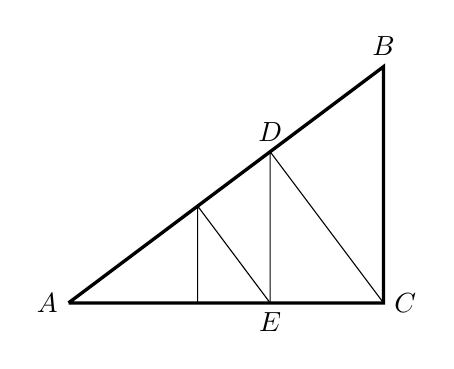
\begin{tikzpicture}[>=latex, scale=1]
        \draw[very thick] (0,0)node[left]{$A$}--(4,0)node[right]{$C$}--(4,3)node[above]{$B$}--(0,0);
        \draw (4,0)--(2.56,1.92)node[above]{$D$}--(2.56,0)node[below]{$E$};
        \draw (2.56,0)--(1.64,1.23)--(1.64,0);
      \end{tikzpicture}
      \caption{}\label{fig:question_triangle}
    \end{minipage}
    \begin{minipage}[t]{0.48\textwidth}
      \centering
      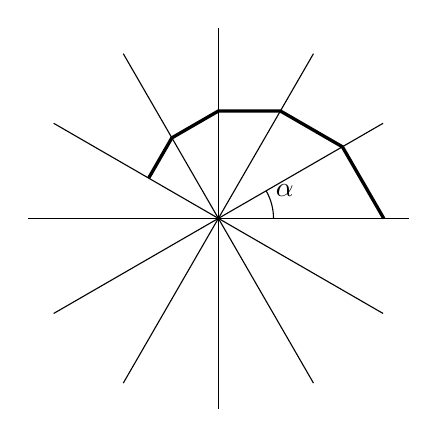
\begin{tikzpicture}[>=latex, scale=.7]
        \foreach \x in {0,1,2,...,11}
        {
            \draw(0,0)--(30*\x:3.45);
        }
        \draw[very thick] (3,0)--(30:0.866*3)--(60:0.866*0.866*3)--(90:0.866*0.866*0.866*3)--(120:0.866*0.866*0.866*0.866*3)--(150:0.866*0.866*0.866*0.866*0.866*3);
        \draw (1,0) arc (0:30:1)node [right]{$\alpha$};
      \end{tikzpicture}
      \caption{}\label{fig:question_ratio}
    \end{minipage}
  \end{figurehere}
  \item 直角三角形三边之长分别为 $3,4,5$,作一圆内切于此三角形,再作一圆外切于此圆,并切于三角形的斜边和边长为 4 的直角边,如此继续作下去,则得到一个切圆的序列,求这些圆的面积之和。
\end{question}
\end{Exercise}

\section{数列极限存在定理}
前面在引进数列极限的定义时,所考虑的许多数列的极限都是已经知道的,然后再用数列极限的定义来验证,如果数列极限的概念仅能给出这样的认识,即一些已知数能够用另一些已知数的某些数列来逼近,那么我们从极限概念所得到的东西太少了。但是数列的一个最为重要的应用在于,有些问题所要确定的数值往往不能用别的方法直接得知或表示,却能用数列极限方式来表示。例如我们用有理数逼近无理数,又在上一节用圆内接正多边形的面积来逼近圆面积,求出 $\uppi$ 的数值等,这样的例子就是数列极限重要应用的典型例子。因此我们构造的数列是否收敛就成为第一位重要问题了。对于一个数列 $\{a_n\}$ 的极限,事实上应该分成两个层次来讨论。

\begin{enumerate}
  \item 存在性。即数列 $\{a_n\}$ 是否有极限存在?
  \item 求值问题。假如已经确定了给定数列 $\{a_n\}$ 的极限存在,我们再设法求它的极限值,其实只要确定了 $\{a_n\}$ 的极限存在,那么这个极限值就是一个实数,而数列 $\{a_n\}$ 就是它的逐次逼近的近似数值,要点是去了解数列的性质,总之求值问题是个比较次要的问题了。 
\end{enumerate}

下面给出一个比较简单的极限存在定理。
\begin{Theorem}[极限存在定理]{定理}
  递增有上界的数列 $\{a_n\}$ 极限存在(同样,递减有下界数列 $\{a_n\}$ 的极限也存在)。
\end{Theorem}
 
{\linespread{1.65}\selectfont
例如:数列 $\left\{\dfrac{n^2-1}{n^2}\right\}$ 符合定理的条件,因为 
$0,\; \dfrac{3}{4},\; \dfrac{8}{9},\; \dfrac{15}{16},\; \dfrac{24}{25},\; \ldots$ 显然是递增的,同时 $a_n=\dfrac{n^2-1}{n^2}=1-\dfrac{1}{n^2}<1$, 也就是说,它是有界的,而且容易看出数列的极限值是 1,事实上\par}
\[\lim_{n\to\infty}\frac{n^2-1}{n^2}=\lim_{n\to\infty}\left(1-\frac{1}{n^2}\right)=1-0=1\]

下面的证明可以说是将二分逼近和实数完备性配合运用的典型例子,在这儿是初次用到,往后还会遇到相似的配合用法。其实,只要能基本上理解命题意义和证明大意,就可以先去学习它的应用,往往用了几次后再回头看第二遍,也就更加明白了。

\begin{proof}
  一个使得 $a_n\leqslant K$ 恒成立的常数 $K$ 叫做 $\{a_n\}$ 的一个\emph{上界}。下面我们将用二分逼近法和完备性来说明 $\{a_n\}$ 的极限等于它的\emph{最小上界}(因为 $\{a_n\}$ 是递增的)。

{\linespread{1.65}\selectfont 令 $A_1=a_1$,$B_1=K$,由假设 $A_1=a_1\leqslant a_n\leqslant K=B_1$,即所有 $a_n$ 都在线段 $[A_1,B_1]$ 之内,将线段 $[A_1,B_1]$ 二等分,假如分点 $\dfrac{1}{2}(A_1+B_1)$ 还是一个上界(即 $a_n\leqslant \dfrac{A_1+B_1}{2}$ 恒成立),则取前半段为 $[A_2,B_2]$,不然则取后半段为 $[A_2,B_2]$。这样逐次二等分,每次当分点 $\dfrac{1}{2}(A_m+B_m)$ 是一个上界时,取其前半段,不然则取其后半段,继续不断地按照上述办法二等分而选取其半段,就得到满足下列性质的两个夹逼数列 $\{A_n\}$ 和 $\{B_n\}$:\par}

\begin{enumerate}
  \item\label{itm:property1} $A_1\leqslant A_2\le A_3\leqslant \cdots \leqslant A_m\leqslant \cdots \leqslant B_m\le \cdots\leqslant B_3\leqslant B_2\leqslant B_1$,$(B_m-A_m)\to 0$
  \item\label{itm:property2} 所有 $B_m$ 都是数列 $\{a_n\}$ 的上界。
  \item\label{itm:property3} 对于任何 $A_m$, 都至少有一个 $a_N$ 使得 $A_m<a_N$,换言之,线段 $[A_m,B_m]$ 至少包含一个点,比如 $a_N$(由 $\{a_n\}$ 的递增性,所有 $n\geqslant N$ 也满足 $A_m<a_n$)。
\end{enumerate}

因此,由性质 \ref{itm:property1} 和实数完备性就得到唯一的实数 $k$,介于一切 $A_m$ 和 $B_m$ 之间,换言之,存在唯一实数 $k$ 使得  $\lim_{m\to\infty}A_m=k=\lim_{m\to\infty}B_m$

现在让我们来说明 $k$ 也就是 $\{a_n\}$ 的极限!设 $\varepsilon$ 是一个任给的正数,因为 $\lim\limits_{m\to\infty}A_m=k=\lim\limits_{m\to\infty}B_m$,所以存在足够大的 $M$, 使得(如\cref{fig:k_between_A_B})
\begin{equation}
    k-\varepsilon<A_M\le k\le B_M<k+\varepsilon
\end{equation}
\begin{figure}
  \begin{tikzpicture}[>=latex]
        \draw[very thick,->] (1,0)--(9,0);    
\foreach \x/\xtext in {5/k,2/k-\varepsilon,8/k+\varepsilon,3.5/A_M,6.5/B_M}
{
    \draw (\x,0)node[below]{$\xtext$}--(\x,.1);
}    
\draw (4.5,0)--(4.5,.1)node[above]{$a_N$};
    \end{tikzpicture}

    \caption{}\label{fig:k_between_A_B}
\end{figure}
由性质 \ref{itm:property3} 知道,存在一个够大的 $N$,使得
\begin{equation}
    A_M<a_N    
\end{equation}
由性质 \ref{itm:property2} 知道,$B_M$ 是一个上界,即恒有
\begin{equation}
    a_N\leqslant B_M
\end{equation} 
由 $\{a_n\}$ 的递增性,当 $n\geqslant N$ 时,有
\begin{equation}
    a_N\leqslant a_n
\end{equation}

综合上述四点,就说明了当 $n\geqslant N$时,有
\[k-\varepsilon<A_M\le a_N\le a_n<B_M<k+\varepsilon\]
亦即 $|a_n-k|<\varepsilon$, 这也就说明了 $\lim\limits_{n\to\infty}a_n=k$。
\end{proof}


\begin{example}
  应用本节存在定理,求 $\displaystyle \lim_{n\to\infty}\frac{r^n}{n!}$。
\end{example}

\begin{solution}
    设 $x_n=\dfrac{r^n}{n!}$,则
\[x_{n+1}=\frac{|r|}{n+1}|x_n|\]
所以只在 $n>|r|-1$ 时,数列 $\{|x_n|\}$ 才是递减的,同时,由于 $|x_n|>0$,所以它是有下界的,因此数列 $\{|x_n|\}$ 收敛于 $\ell$,在上面等式两边取极限
\[\lim_{n\to\infty}|x_{n+1}|=\lim_{n\to\infty}\frac{|r|}{n+1}\cdot |x_n|\]
即
\[\lim_{n\to\infty}|x_{x+1}|=\lim_{n\to\infty}\frac{|r|}{n+1}\cdot \lim_{n\to\infty}|x_n|\]
因为变量 $|x_{n+1}|$ 和 $|x_n|$ 取同一个数列的数值(除第一个数值外)。因此有同一个极限 $\ell$,即:$\ell=0\cdot \ell$,所以
\[\lim_{n\to\infty}|x_n|=\ell=0\]
最后有
\[\lim_{n\to\infty} x_n=\lim_{n\to\infty} \frac{r^n}{n!} =0\]
\end{solution}

\begin{example}
    求下面数列$\{a_n\}$:
\[\begin{split}
   &  a_1=\sqrt{2},\quad a_2=\sqrt{2+\sqrt{2}},\quad a_3=\sqrt{2+\sqrt{2+\sqrt{2}}},\\
    & \ldots,\quad a_n=\underbrace{\sqrt{2+\sqrt{2+\cdots+\sqrt{2}}}}_{\text{$n$个根号}},\quad\ldots
\end{split} \]
的极限。
\end{example}
   
\begin{solution}
显然,$a_1=\sqrt{2},\;a_2=\sqrt{2+a_1},\;\ldots,\;
a_n=\sqrt{2+a_{n-1}},\;\ldots$

$\because\quad 2+\sqrt{2}>2,\qquad \therefore\quad a_2=\sqrt{2+\sqrt{2}}>\sqrt{2}=a_1$

又假设 $a_n>a_{n-1}$ 成立,则 $2+a_n>2+a_{n-1}$

$\therefore\quad a_{n+1}=\sqrt{2+a_n}>\sqrt{2+a_{n-1}}=a_n$

因此,对于一切 $n\in\mathbb{N}$,有 $a_{n+1}>a_n$,则此数列是递增的。

$\because\quad \sqrt{2}<2,\qquad \therefore\quad a_1<2,\quad a_2<\sqrt{2+2}=2$

假设 $a_{n-1}<2$,那么,
\[a_n=\sqrt{2+a_{n-1}}<\sqrt{2+2}=2\]
所以对于一切 $n\in\mathbb{N}$, 有 $a_n<2$ 。

根据极限存在定理知数列 $\{a_n\}$ 有极限,设它为 $x$,于是,
$\lim\limits_{n\to\infty}a_n=x$。
由于
\[a_n=\sqrt{2+a_{n-1}}\]
两边平方得
\[a^2_n={2+a_{n-1}}\]
取极限有
\[\lim_{n\to\infty}a^2_n =\lim_{n\to\infty}(2+a_{n-1})\]
或者:$x^2=2+x$,解得:
\[x_1=2,\qquad x_2=-1\]
然而 $\because\quad a_n>0\quad \Longrightarrow\quad \lim\limits_{n\to\infty}a_n=x\geqslant 0$,$\therefore\quad x_2=-1$ 不合要求,因此,
\[\lim_{n\to\infty}a_n=2\]
\end{solution}

由上面的极限存在定理可以引出下面的结论:
\begin{enumerate}
  \item 预先证明极限存在是很重要的,它也给实际计算这个极限提供了基础。
  \item 在极限定义中,要求我们预先猜到 $\{a_n\}$ 的极限值 $A$, 然后再用数列极限定义来验证这个极限 $A$ 是存在的,这就和前面所说的在数列极限的重要应用中出现的层次有些本末倒置,本节的极限存在定理就纠正了这种本末倒置的局面。
\end{enumerate}

\begin{Exercise}
\begin{question}
  \item 试利用关于单调而有界的数列的极限存在定理检验下面数列极限存在性。
  \begin{tasks}
    \task $a_n=1+\dfrac{1}{1\cdot 2}+\dfrac{1}{1\cdot 2\cdot 3}+\cdots+\dfrac{1}{1\cdot 2\cdot 3\cdots (n-1)}$,\quad $n=1,2,3,\ldots$
    \task $a_n=\dfrac{1}{n+1}+\dfrac{1}{n+2}+\cdots +\dfrac{1}{2n}$,\quad $n=1,2,3,\ldots$
    \task $x_n=p_0+\dfrac{p_1}{10}+\cdots +\dfrac{p_n}{10^n}$,式中 $p_i,\; (i=0,1,2,\ldots)$ 是非负数,且从 $p_1$ 起不大于 9。
  \end{tasks}
  \item 已知 $a_1=\sqrt{2},\; a_2=\sqrt{2\sqrt{2}},\; a_3=\sqrt{2\sqrt{2\sqrt{2}}},\ldots,a_{n+1}=\sqrt{2a_n},\ldots$, 求 $\lim\limits_{n\to\infty}a_n$。
  \item 设 $a_{n+1}=\sqrt{k+a_n}$, 这里 $k>0$,$a_1>0$,求证数列 $\{a_n\}$ 递增,并以方程 $x^2=x+k$ 的正根为极限。
  \item 已知 $x_1=1,x_2=1+\dfrac{x_1}{1+x_1},\ldots,x_n=1+\dfrac{x_{n-1}}{1+x_{n-1}},\ldots$, 求 $\lim\limits_{n\to\infty}x_n$。
  \item 数列 $\{x_n\}$ 由下面递归方程定义
  \[x_1=h,\qquad x_{n+1}=x_n^2+k\]
  这里 $0<k<\dfrac{1}{4}$,$h$ 在方程 $x^2-x+k=0$ 的二根 $a,b$ 之间,即 $a<h<b$。求证:$a<x_{n+1}<x_n<b$,并求 $\lim\limits_{n\to\infty}x_n$。
  \item 设 $0<a_1<b_1$ 是两个给定正数,令 
  \[\begin{split}
    a_2&=\sqrt{a_1b_1},\qquad b_2=\frac{1}{2}(a_1+b_1),\quad (a_2<b_2)\\
    a_3&=\sqrt{a_2b_2},\qquad b_3=\frac{1}{2}(a_2+ b_2),\quad (a_3<b_3)\\
    \cdots \\
    a_{n+1}&=\sqrt{a_nb_n},\qquad b_{n+1}=\frac{1}{2}(a_n+b_n),\quad (a_{n+1}<b_{n+1})\\
  \end{split}\]
  求证:
  \begin{tasks}
    \task $\{a_n\}$ 递增和 $\{b_n\}$ 递减;
    \task $\{a_n\}$ 和 $\{b_n\}$ 的极限相同。
  \end{tasks}
\end{question}
\end{Exercise}
\chapter{单变量函数}
前面中我们已经说明了如何由量的度量而产生实数系。在这一章中我们要进一步说明如何用变数符号去表达变量,用变数之间的函数关系去表达变量之间的关联。变数是变量的抽象,函数是变量相互关系的抽象。在这一章里我们还要运用极限来分析和确立连续函数的概念。

\section{函数的概念}
\subsection{变数和变域}
在研究自然现象时,人们会遇到许多不同的物理量,如时间、长度、体积、速度、质量、力等等。按照给定条件,能取许多不同数值的量叫做\emph{变量};而只取一个数值的量叫做\emph{常量},用来表达变量的符号叫做\emph{变数}。习惯上常用 $x,y,z$等字母表示变数,从纯数学的观点来说,一个变数就是一个“能取许多不同数值”的符号,它所能取的所有数值构成一个集合,叫做它的\emph{变域}。如果变数 $x$ 的变域已经给出,我们就认为变数 $x$ 是已知的。一般说来,任何数集可以当作变数的变域。常会遇到取所有自然数的变数 $n$,譬如数列中的项数。可是在现实生活中,我们通常研究的是连续变化的变数,如动点所经过的路程及所花的时间等物理量,就是这种变数的原形,数的区间就是这一类变数的变域,最常用的区间是以两个实数 $a$ 与 $b$($a<b$)——它的两个端点——为界限的有限区间,两个端点本身可以包含在区间内,也可以不包含在内。因此我们可以把区间分为:
\begin{itemize}
    \item 开区间 $(a,b)$ 就是 $\{x|a<x<b\}$;
    \item 闭区间 $[a,b]$ 就是 $\{x|a\leqslant x\leqslant b\}$;
    \item 半开区间 $(a,b]$ 就是 $\{x|a<x\leqslant b\}$;$[a,b)$ 就是 $\{x|a\leqslant x<b\}$。
\end{itemize}
在上述各种情形,数 $b-a$ 为区间的长度。

常量可以看作变量的特殊情形,它的变域是由一个数组成的集合 $\{x|x=a\}$。

数轴上的线段是数的区间的几何表示,图示开区间如\cref{fig:open_interval1} 或\cref{fig:open_interval2}。

在点 $a,b$ 处的圆圈或圆括号表示从区间去掉这两个数。在两个圆圈之间的粗线段表示在$a,b$ 之间的一切数 $x$。图示闭区间如\cref{fig:close_interval}。图示半开区间如\cref{fig:semi_open_interval1,fig:semi_open_interval2},每一种情形都只包含出现有方括号的数,以及在 $a,b$ 之间的一切实数。
\begin{figure}
  \begin{minipage}[t]{0.48\textwidth}
    \centering
    \begin{tikzpicture}[>=latex, scale=.7]
      \draw[->] (0.5,0)--(7.5,0);
      \draw[ultra thick] (2.5,0)node[below=5pt]{$a$}--(5.5,0)node[below=5pt]{$b$};
      \draw (2.5,0)[fill=white] circle (2pt);
      \draw (5.5,0)[fill=white] circle (2pt);
    \end{tikzpicture}
    \caption{}\label{fig:open_interval1}
  \end{minipage}
  \begin{minipage}[t]{0.48\textwidth}
    \centering
    \begin{tikzpicture}[>=latex, scale=.7]
      \draw[->] (0.5,0)--(7.5,0);
      \draw[ultra thick] (2.5,0)node[below=5pt]{$a$}--(5.5,0)node[below=5pt]{$b$};
      \node at (2.5,0){$($}; \node at (5.5,0){$)$};
    \end{tikzpicture}
    \caption{}\label{fig:open_interval2}
  \end{minipage}
  \begin{minipage}[t]{0.48\textwidth}
    \centering
    \begin{tikzpicture}[>=latex, scale=.7]
      \draw[->] (0.5,0)--(7.5,0);
      \draw[ultra thick] (2.5,0)node[below=5pt]{$a$}--(5.5,0)node[below=5pt]{$b$};
      \node at (2.5,0){$[$}; \node at (5.5,0){$]$};
    \end{tikzpicture}
    \caption{}\label{fig:close_interval}
  \end{minipage}
  \begin{minipage}[t]{0.48\textwidth}
    \centering
    \begin{tikzpicture}[>=latex, scale=.7]
      \draw[->] (0.5,0)--(7.5,0);
      \draw[ultra thick] (2.5,0)node[below=5pt]{$a$}--(5.5,0)node[below=5pt]{$b$};
      \node at (2.5,0){$($}; \node at (5.5,0){$]$};
  \end{tikzpicture}
    \caption{}\label{fig:semi_open_interval1}
  \end{minipage}
  \begin{minipage}[t]{0.48\textwidth}
    \centering
    \begin{tikzpicture}[>=latex, scale=.7]
      \draw[->] (0.5,0)--(7.5,0);
      \draw[ultra thick] (2.5,0)node[below=5pt]{$a$}--(5.5,0)node[below=5pt]{$b$};
      \node at (2.5,0){$[$}; \node at (5.5,0){$)$};
    \end{tikzpicture}
    \caption{}\label{fig:semi_open_interval2}
  \end{minipage}
  \begin{minipage}[t]{0.48\textwidth}
    \centering
    \begin{tikzpicture}[>=latex, scale=.7]
      \draw[->] (0.5,0)--(7.5,0);
      \draw[ultra thick] (2.5,0)node[below=5pt]{$a$}--(5.5,0)node[below=5pt]{$b$};
      \node at (2.5,0){$($}; \node at (5.5,0){$)$};
      \draw (4,0)[fill=white] circle (2pt)node[above]{$c$};
    \end{tikzpicture}
    \caption{}\label{fig:without_center_interval}
  \end{minipage}
\end{figure}

有时也要考虑无穷区间,用符号 $-\infty,+\infty$ 作为一端或两端,它们的记号和上面所引进的相类似,例如 $(-\infty,+\infty)$ 是全体实数集合 $\{x|x\in\mathbb{R}\}$, 区间 $(a,+\infty)$ 表示集合 $\{x|x>a\}$,区间 $(-\infty,b]$ 表示集合 $\{x|x\leqslant b\}$。无穷区间在几何上可用两端无限伸延的直线或一端无限伸延的射线来
表示。

以后我们要常用到一点的邻域的概念。\emph{$c$ 点的邻域}是包含 $c$ 点的任何开区间 $(a,b)$, 而 $c$ 点的去心邻域指去掉 $c$ 点的任何 $c$ 点的邻域。它的图象如\cref{fig:without_center_interval}。

$c$ 点的去心邻域可写成 $(a,c)\cup (c,b)$。我们常把 $c$ 点的邻域写成对称的形式:$(c-r,c+r)$,对任何 $r>0$, 并且称它为\emph{$c$ 点的对称邻域}。

\begin{example}
  试写出含于区间 $(1,5)$ 中 $\uppi$ 的对称邻域。
$\left(\uppi-\dfrac{1}{2},\uppi+\dfrac{1}{2}\right)$ 是含于 $(1,5)$ 的 $\uppi$ 对称邻域。此外 $(\uppi-1,\uppi+1)$,$\left(\uppi-\dfrac{3}{2},\uppi+\dfrac{3}{2}\right)$,$(\uppi-0.01,\uppi+0.01)$ 等都是含于 $(1,5)$ 中的对称邻域。
\end{example}

\subsection{函数的定义}
我们已经在第三册研究过许多函数,例如多项式函数、
三角函数,由于函数这个概念的重要性,并且它将是我们
的主要研究对象,因此需要回忆一般的函数的定义,下面我
们从数集之间的多对一(包括一对一)的关系重新给出函数
定义。

\begin{Definition}
设有数集 $A,B$,如果有一对应关系或法则 $f$ 存在,对于 $A$ 的任何一个数 $x$,有数集 $B$ 中唯一的一个数 $y$ 与之对应,我们就称给出了一个从数集 $A$ 到数集 $B$ 内的函数 $f$,用
\[f:A\mapsto B\]
表示,并写成 $y=f(x),\; (x\in A)$,此时称 $f(x)$ 为函数 $f$ 在 $x$ 的函数值,并称 $A$ 为函数 $f$ 的\emph{定义域}。又当 $x$ 取遍 $A$ 中的数时,函数值 $f(x)$ 全体也构成一个数集,称为函数 $f$ 的\emph{值域},记作
\[f(A)=\{f(x)|x\in A\}\]
要注意的是在构造一个函数 $f:A\mapsto B$ 的时候,$f(A)$ 不一定等
于 $B$, 而是 $B$ 的一个真子集,即 $f(A)\subset B$。
\end{Definition}



\begin{example}
设 $\mathbb{R}$ 是实数集,函数 $f:\mathbb{R}\mapsto\mathbb{R}$ 定义为
\[f(x)=\frac{2x}{x^2+1},\quad x\in(-\infty,+\infty)\]
求它的值域。
\end{example}

\begin{solution}
    方程 $f(x)=\dfrac{2x}{x^2+1}$ 等价于
    \begin{equation}
      \label{eq:function}
        yx^2-2x+y=0
    \end{equation}
根据函数的值域定义,任给 $y\in f(\mathbb{R})$, 方程 \eqref{eq:function} 必有实数
解,而方程 \eqref{eq:function} 有实数解的充要条件是
\[\Delta=1-y^2\geqslant 0\]
即:$-1\leqslant y\leqslant 1$,所以
\[f(\mathbb{R})=\{f(x)|-1\leqslant f(x)\leqslant 1\}\subset \mathbb{R}\]
\end{solution}

在函数的定义中包含三个要素,即\emph{定义域},\emph{多对一的对应法则}和\emph{函数值所在的数集}。应养成一个习惯,当给定一个函数时,必须指明它的定义域。在实际问题中,函数的定义域是根据实际意义来确定的,例如温度计刻有华氏温标度数 $F$ 和摄氏温标度数 $c$,因为不存在低于绝对零度的温度,因此,这两个度数之间的函数 $\varphi$ 是
\[F=\varphi(c)=\frac{9}{5}c+32,\quad c\in (-273,+\infty)\]

以后,当我们只在数学上,一般地研究一个具体解析式子规定的函数关系时,如果定义域$A$ 没有被指明,那么函数的定义域是使解析式子具有数值意义的所有 $x$ 的数值组成的
自然定义域,函数 $y$ 的值域通常是不指出的,因为由对应的规律本身就可以确定函数的值域。

\begin{example}
  求下列函数定义域:
\begin{tasks}(2)
  \task $f(x)=\dfrac{\sqrt{1-x}}{x}$
  \task $g(x)=\sqrt{x^2-1}$
\end{tasks}
\end{example}

\begin{solution}
    \begin{enumerate}
        \item \[\text{函数$f$有意义}\Leftrightarrow \begin{cases}
    1-x \geqslant 0\\
    x\ne 0
\end{cases}\Rightarrow\quad x\leqslant 1, \quad x\ne 0\]
$\therefore\quad $ 函数 $f$ 的定义域为 $(-\infty,0)\cup(0,1]$。

\item \[\text{函数$g$有意义}\Leftrightarrow x^2-1\geqslant 0 \Rightarrow\quad x\leqslant 1, \text{ 或 } x\geqslant 1\]
$\therefore\quad $ 函数 $g$ 的定义域为$(-\infty,-1]\cup[1,+\infty)$。
    \end{enumerate}
\end{solution}

\subsection{相等的函数}
怎样的两个函数是相等的函数?在数学中,有些函数可以用不同的方式来定义,例如,函数 $f:\mathbb{R}\mapsto \mathbb{R}^+\cup\{0\}$ 是由 $f(x)=|x|$ 规定的,而函数 $g:\mathbb{R}\mapsto \mathbb{R}^+\cup\{0\}$ 是由 $g(x)=\sqrt{x^2}$ 规定的,这里表示 $f(x)$ 与 $g(x)$ 的式子全不同,但是对于它们的相同的定义域中的任一 $x$ 值,经过不同规则的计算,它们的结果是相同的,即 $f(x)=g(x)$, 所以对于这个例子来说,尽管函数 $f(x),g(x)$ 的表达式不同,我们说 $f(x)$ 和 $g(x)$ 表示相同的函数。此外,解析式子相同,但定义域不同的函数是不相同的函数。例如:
\[\begin{split}
    f_1(x)&=\frac{1}{x},\qquad x\in (-\infty,0)\cup(0,+\infty)\\
    f_2(x)&=\frac{1}{x},\qquad x\in (0,+\infty)\\
    f_3(x)&=\frac{1}{x},\qquad x\in (0,1)
\end{split}\]
是不相同的函数,因为对于 $x=-2$, $f_1$ 有意义而 $f_2,f_3$ 都无
意义;对于 $x=2$, $f_1$ 和 $f_2$ 都有意义而 $f_3$ 无意义。

下面给出相等(同)的两个函数的条件。
\begin{Definition}{定义}
两个函数 $f:A\mapsto B$, $g:C\mapsto D$ 称为相等的当且仅当 $A=C$,$B=D$,且对于每个 $a\in  A$(或 $C$),有 $f(a)=g(a)$。
\end{Definition}

读者可能会不同意上面 $B=D$ 这个条件,提出下面这个例子来反驳:

“由 $f(n)=g(n)=n$ 给出的两个函数 $f:\mathbb{N}\mapsto\mathbb{N}$,$g: \mathbb{N}\mapsto \mathbb{Q}$ 是相等的函数”我们须指出两个函数不同的地方,就
函数值所在数集上看,$g$ 可以除以 2, 因此,对于 $g$ 我们可以构造一个新函数,
$\dfrac{1}{2}g:\mathbb{N}\mapsto \mathbb{Q}$, 这里
\[\left(\frac{1}{2}g\right)(n)=\frac{1}{2}n\]
但是对于 $f$, 不能做这种构造。

\subsection{函数的几个类型——满射、单射和双射}
现在,我们来讨论函数的三个重要类型,先给出定义,然后再举例说明。

\begin{Definition}
  如果在函数 $f:A\mapsto B$ 的 $B$ 中的每一个数 $b$ 在函数 $f$ 的作用下都是 $A$ 中一个数或某些数的对应数,也就是说:对于任意 $b\in B$,存在一个 $a\in A$,使得 $b=f(a)$,这样我们就说 $f$ 是由 $A$ 到 $B$ 的\emph{满射}。
\end{Definition}

显然,如果 $f:A\mapsto B$ 是满射,那么 $f(A)=B$。

第二类函数和满射同样地重要,叫做\emph{单射},定义如下:

\begin{Definition}
  如果对于 $A$ 中的任何两个不同的数 $a_1$ 和 $a_2$,就在 $B$ 中有两个不同的函数值 $f(a_1)$ 和 $f(a_2)$,即任何 $a_1,a_2\in A$,$a_1\ne a2\Rightarrow f(a_1)\ne f(a_2)$,那么我们就说 $f:A\mapsto B$ 是\emph{单射}(或一对一)。
\end{Definition}

 
它的逆否命题“如果在 $B$ 中有 $f(a_1)=f(a_2)$ 就在 $A$ 中有
$a_1=a_2$, 那么函数 $f:A\mapsto B$叫做\emph{单射}(或一对一)。”和上面
的定义等价,也常用来说明函数是一对一的。

还有一类很重要的函数叫做\emph{双射}。

\begin{Definition}
  函数 $f:A\mapsto B$,如果是满射又是单射,就叫做\emph{双射}。
\end{Definition}

\begin{example}
  函数 $f:\mathbb{R}\mapsto [-1,1]$,这里 $f(x)=\sin x, x\in\mathbb{R}$
是满射,但不是单射,因为对于 $\sin x=\dfrac{1}{2}\in [-1,1]$,
就有无穷多个 $x=\dfrac{\uppi}{6}+2k\uppi$ 或 $\dfrac{5\uppi}{6}+2k\uppi\;(k\in\mathbb{Z})$ 的值和它对应。
\end{example}

\begin{example}
  函数 $f:\mathbb{N}\mapsto\mathbb{N}$,这里 $f(n)=2n$ 是单射,但不是满射。
\end{example}

\begin{example}
  设 $2\mathbb{N}$ 代表偶数集,函数 $f:\mathbb{N}\mapsto 2\mathbb{N}$,这里$f(n)=2n$ 就是一双射。
\end{example}

\section{函数的运算与复合函数}

\subsection{函数的四则运算}

设 $f(x),g(x)$ 是两个 $x$ 的函数,它们的定义域分别为 $D_f$ 和 $D_g$,我们可以用通常对于“数”的四则运算得到它们的和函数 $(f+g)(x)$,差函数 $(f-g)(x)$,积函数 $(f\cdot g)(x)$ 与商函数 $\frac{f}{g}(x),\; g(x)\ne 0$。它们的定义域为 $D_f\cap D_g$。

由 $f(x),g(x)$ 的四则运算所得出来的新函数的定义如下:
\begin{itemize}[itemsep=7pt]
  \item $(f+g)(x)=f(x)+g(x)$ (即 $(f+g)$ 在 $x$ 点的值是 $f$,$g$ 的值的和);
  \item $(f-g)(x)=f(x)-g(x)$ (即 $(f-g)$ 在 $x$ 点的值是 $f$,$g$ 的值的差);
  \item $(f\cdot g)(x)=f(x)\cdot g(x)$ (即 $(f\cdot g)$ 在 $x$ 点的值是 $f$,$g$ 的值的积);
  \item $(f/g)(x)=f(x)/g(x)$ (即 $f/g$ 在 $x$ 点的值是 $f$,$g$ 的值的商,但只有在 $g(x)\ne 0$ 时才有意义)。
\end{itemize}

$f+g$, $f-g$ 和 $f\cdot g$ 的定义域是 $f$ 的定义域和 $g$ 的定义域的交集。而 $f/g$ 的定义域要从 $f$ 和 $g$ 的定义域的交集中去掉使 $g(x)=0$ 的值。

\begin{example}
  已知 $f(x)=\sqrt{x}$, $g(x)=\sqrt{1-x}$, 求 $f+g$,$f-g$,$f\cdot g$,$\dfrac{f}{g}$,$\dfrac{g}{f}$。
\end{example}

\begin{solution}
    $f$ 和 $g$ 的自然定义域是 $D_f=\{x|x\geqslant 0\}$, $D_g=\{x|x\leqslant 1\}$,$D_f$ 和 $D_g$ 的交集是 $D_f\cap D_g=[0,1]$。
\begin{itemize}[itemsep=7pt]
    \item 和:$(f+g)(x)=\sqrt{x}+\sqrt{1-x}$
    \item 差:$(f-g)(x)=\sqrt{x}-\sqrt{1-x}$
    \item 积:$(f\cdot g)(x)=\sqrt{x(1-x)}$
    \item 商:$\dfrac{f}{g}(x)=\sqrt{\dfrac{x}{1-x}},\qquad \dfrac{g}{f}(x)=\sqrt{\dfrac{1-x}{x}}$
\end{itemize}

$f+g$, $f-g$, $f\cdot g$ 的定义域是 $[0,1]$。因为当 $x=1$ 时,$g(x)=0$, 所以 $\dfrac{f}{g}$ 的定义域是 $[0,1)$, 同样得到 $\dfrac{g}{f}$ 的定义域 $(0,1]$。
\end{solution}

\begin{example}
设$f(x)=\sin x$, $g(x)=\cos x$,$D_f=(-\infty,+\infty)$,$D_g=(-\infty,+\infty)$,则:
\[\begin{split}
    (f+g)(x)=\sin x+\cos x&=\sqrt{2}\left(\frac{1}{\sqrt{2}}\sin x+\frac{1}{\sqrt{2}}\cos x\right)\\
    &=\sqrt{2}\left(\sin x\cos\frac{\uppi}{4}+\cos x\sin\frac{\uppi}{4} \right)\\
    &=\sqrt{2}\sin\left(x+\frac{\uppi}{4}\right)\\
    (f-g)(x)=\sin x-\cos x&=\sqrt{2}\sin\left(x-\frac{\uppi}{4}\right)\\
    (f\cdot g)(x)=\sin x\cdot \cos x&=\frac{1}{2}\sin 2x\\
    \left(\frac{f}{g}\right)(x)=\frac{\sin x}{\cos x}&=\tan x\\
\end{split}\]    

这里 $f+g$, $f-g$, $f\cdot g$ 的定义域是 $(-\infty,+\infty)$,$\dfrac{f}{g}$ 的定义域是
\[\left\{x\big|x\in\mathbb{R},\; x\ne \frac{\uppi}{2}+k\uppi,\; k\in \mathbb{Z}\right\}\]
\end{example}

\subsection{复合函数}
上面我们是用四则运算来组合已知函数为一个新函数的,但是构成新的函数的方法,还有一个更重要的运算叫做组成函数的函数或复合函数法。

我们先从一个简单的例子说起,火箭从地面上的 $L$ 点垂直向上发射,火箭 $R$ 在 $t$ 秒后离开发射点的距离是 $h(t)$, 这个函数是已知的。在离发射座 \qty{1}{km} 远的地方有一个观测站 $O$,我们要求把火箭与观测站的距离 $d$ 确定为时间 $t$ 的函数(\cref{fig:function_d_vs_t})。
\begin{figure}
\begin{tikzpicture}[thick]
\draw (0,0)node[below]{$L$}--node[below]{1}(4,0)node[below]{$O$}--node[above]{$d$}(0,2.0)node[above]{$R$}--node[left]{$h$}(0,0);
\end{tikzpicture}
    \caption{}\label{fig:function_d_vs_t}
\end{figure}

我们已经知道火箭的垂直高度 $h$ 是 $t$ 的函数 $h(t)$,又火箭到观测站的距离 $d$ 又是火箭的高度 $h$ 的函数
\[d=\sqrt{1+h^2}\]
因此在时刻 $t$,$R$ 到 $O$ 的距离是
\[d(t)=\sqrt{1+h^2(t)}\]

上面函数 $d(t)$ 是由 $h=h(t)$ 和 $d=f(h)=\sqrt{1+h^2}$ 两个函数构成的,把其中一个函数 $h(t)$ 代入另一个函数 $f(h)$ 的运算叫做复合运算,得到的函数 $d(t)=f\big(h(t)\big)$ 叫做 $t$ 的复合函数。

一般说来,若 $z=f(y)$, $y=g(x)$,且 $g(x)$ 的值域含于 $f(y)$ 的定义域中,那么对于 $g(x)$ 定义域内的每一个 $x$ 值经过中间变数 $y$,相应地得到唯一确定的一个值$z$,变数 $z$ 经过中间变数 $y$ 而成变数 $x$ 的函数,记为 $z=f\big(g(x)\big)$,这个函数称为前两个函数的\emph{复合函数}。应该指出,函数 $y=g(x)$ 的值域不能超出函数 $f(y)$ 的定义域,这是极重要的。


\begin{example}
    设 $z=\sqrt{1+y}$, 它的定义域 $D_y=[-1,+\infty)$,再设 $y=x^2-5$,它的定义域 $D_x=(-\infty,+\infty)$, 值域 $R=[-5,+\infty)$。

作为复合函数 $z=\sqrt{1+(x^2-5)}=\sqrt{x^2-4}$,其定义域只能是 $(-\infty,-2]$ 和$[2,+\infty)$,这时,$y=x^2-5$ 的值域是 $[-1,+\infty)$, 它没有超过 $D_y=[-1,+\infty)$ 的范围,这就是说复合函数 $z=f\big(g(x)\big)$ 的定义域只能由 $y=
g(x)$ 的定义域中那些使 $g(x)$ 属于 $z=f(y)$ 的定义域的 $x$ 组成。
\end{example}

\begin{example}
已知 $f(g)=\dfrac{1}{g+1}$,$g=g(x)=x^2$。

求 $f\big(g(x)\big)$ 和 $g\big(f(x)\big)$。    
\end{example}

\begin{solution}
\[\begin{split}
    f\big(g(x)\big)&=\frac{1}{x^2+1}\\
    g\big(f(x)\big)&=\left(\frac{1}{x+1}\right)^2=\frac{1}{x^2+2x+1}
\end{split}\]
显然,$f\big(g(x)\big)\ne g\big(f(x)\big)$, 这表明函数的复合运算是不满足交换律的。
\end{solution}

\begin{example}
已知 $f\left(\sin\dfrac{x}{2}\right)=\cos x+1$,
求 $f\left(\cos\dfrac{x}{2}\right)$。
\end{example}    

\begin{solution}
复合函数 $f\left(\sin\dfrac{x}{2}\right)=\cos x+1=2-2\sin^2\dfrac{x}{2}$ 是把函数 $y=\sin\frac{x}{2}$ 代入 $f(y)=2-2y^2$ 中复合而成。现在令 $y=\cos\dfrac{x}{2}$ 代入 $f(y)$,得到
\[f\left(\cos\frac{x}{2}\right)=2-2\cos^2\frac{x}{2}=2-(1+\cos x)=1-\cos x\]
\end{solution}    

在函数的运算中,我们介绍了函数的加、减、乘、除和函数的复合五种运算,从定义来看,我们可以用上述五种运算,由某一简单而基本的函数去造出多种多样的新函数来,譬如从常数函数 $y=c$ 和恒等函数 $y=x$,用加、减、乘运算就可以得出多项式函数。其实我们常常要用到的,并不是把所给的函数组合成更复杂的函数;而是要把所给的函数分解成更简
单的函数的组合,把要解的问题归于比较简单的问题去解决。

\begin{example}
    将函数 $y=x\sin\dfrac{1}{x}$ 分解成比较简单的函数的组合(引进新的中间变数符号)。
\end{example}

\begin{solution}
$y=x\sin\dfrac{1}{x}$ 可分解为 $f(x)=x$ 与 $g(x)=\sin\dfrac{1}{x}$ 之积,又$g(x)=\sin\dfrac{1}{x}$ 可以看作是 $g(h)=\sin h$ 和 $h=h(x)=\dfrac{1}{x}$ 的复合函数,于是原来的函数可以看作下面简单函数的组合
\[F(x)=f(x)\cdot g\big(h(x)\big)\]
这里 $f(x)=x$,$g(h)=\sin h$,$h=h(x)=\dfrac{1}{x}$。    
\end{solution}

\begin{example}
求函数 $\sqrt{x-\sqrt{x+1}-2}$ 的定义域。
\end{example}

\begin{solution}
设 $F(x)=\sqrt{x-\sqrt{x+1}-2}=\sqrt{(x+1)-\sqrt{x+1}-3}$,则 $F(x)$ 可以看作$f(y)=\sqrt{y^2-y-3}$ 与 $y=g(x)=\sqrt{x+1}$ 的复合函数,即$F(x)=f\big(g(x)\big)$ 且知:

$f(y)$ 的定义域 $D_f=\left(-\infty,\dfrac{1-\sqrt{13}}{2}\right]\bigcup\left[\dfrac{1+\sqrt{13}}{2},+\infty\right)$

$g(x)$ 的定义域 $D_g=[-1,+\infty)$, 它的值域$R_x=[0,+\infty)$

\[\begin{split}
&\text{复合函数 $F(x)=f\big(g(x)\big)$有意义}\Longleftrightarrow
\begin{cases}
    g(x)\text{有意义}\\
    g(x)\in\left[\dfrac{1+\sqrt{13}}{2},+\infty\right)
\end{cases}\\
&\Longleftrightarrow
\begin{cases}
    x+1\geqslant 0\\
    \sqrt{x+1}\geqslant \dfrac{1+\sqrt{13}}{2}
\end{cases}\Longleftrightarrow
\begin{cases}
    x\geqslant -1\\
    x+1\geqslant \left(\dfrac{1+\sqrt{13}}{2}\right)^2=\dfrac{7+\sqrt{13}}{2}
\end{cases}\\
&\Longleftrightarrow x\geqslant \frac{5+\sqrt{13}}{2}
\end{split}\]
$\therefore\quad $ 函数 $\sqrt{x-\sqrt{x+1}-2}$ 的定义域是
$\left[\dfrac{5+\sqrt{13}}{2},+\infty\right)$。

如果直接求$F(x)=\sqrt{x-\sqrt{x+1}-2}$的定义域,那
么只须:
\[\begin{split}
   x-\sqrt{x+1}-2\geqslant 0& \Longleftrightarrow x-2\geqslant \sqrt{x+1} \Longleftrightarrow \begin{cases}
    x-2\geqslant 0\\ x+1\geqslant 0\\ (x-2)^2\geqslant (x+1)
\end{cases}\\
& \Longleftrightarrow \begin{cases}
    x\geqslant 2\\x\geqslant -1\\ x\geqslant \dfrac{5+\sqrt{13}}{2}
\end{cases} \Longleftrightarrow x\geqslant \frac{5+\sqrt{13}}{2}
\end{split}\]
$\therefore\quad $ 函数 $\sqrt{x-\sqrt{x+1}-2}$ 的定义域是
$\left[\dfrac{5+\sqrt{13}}{2},+\infty\right)$。
\end{solution}

\begin{Exercise}

\begin{question}
  \item 试确定下面每一对函数 $f$ 和 $g$ 的自然定义域,并求 $f+g$, $f-g$, $f\cdot g$, $f/g$ 和 $g/f$ 的相应的定义域。
  \begin{tasks}(2)
    \task $f(x)=x,\qquad g(x)=\sqrt{x-1}$
    \task $f(x)=\frac{1}{x-2},\qquad g(x)=\frac{1}{\sqrt{x-1}}$
    \task $f(x)=\sqrt{x},\qquad g(x)=\sqrt[4]{x+1}$
    \task $f(x)=\sin x,\qquad g(x)=\cos x$
    \task $f(x)=\tan x,\qquad g(x)=\tan x$
  \end{tasks}
    \item 证明函数 $f(x)=\dfrac{1}{1+x}$ 在它的定义域上是单射的。又 $x$ 为何值时,下列各式才有意义?
\begin{tasks}(2)
    \task $f\big(f(x)\big)$
    \task $f\left(\dfrac{1}{x}\right)$
    \task $f(cx)$
    \task! 对于哪些数 $c$,有一数 $x$ 能使 $f(cx)=f(x)$
\end{tasks}        

\item 下列函数能否构成复合函数 $y=f\big(\varphi(x)\big)$,如果能够
构成,则指出复合函数的定义域和值域:
\begin{tasks}
    \task $y=f(u)=2u+1,\qquad u=\varphi(x)=x^2$
    \task $y=f(u)=\sqrt{u},\qquad u=\varphi(x)=1-x^2$
    \task $y=f(u)=u^2+u^3, \qquad u=\varphi(x)=\begin{cases}
        1,& \text{当 $x$ 为有理数}\\
        2,&\text{当 $x$ 为无理数}\\
    \end{cases}$
    \task $y=f(u)=2$,定义域为 $U_1$,\qquad  $u=\varphi(x)$,定义域为 $X$,值域为 $U_2$。
\end{tasks}

\item 设$f(x)=ax^2+bx+c$,证明
$f(x+3)-3f(x+2)+3f(x+1)-f(x)=0$。
\item 
\begin{tasks}
\task 设 $y=f(x)=a+bx+\dfrac{c}{x}$,求 $f\left(\dfrac{2}{x}\right)$。
\task 设 $y=f(x)=\sqrt{1+x+x^2}$,求 $f(x^2)$, $f(-x^2)$。
\end{tasks}

\item 若 $\varphi(x)=x^3+1$,求 $\varphi(x^2)$,$\big(\varphi(x)\big)^2$, $\varphi\big(\varphi(x)\big)$。
\item 求下列函数定义域:
 \begin{tasks}(2)
    \task $y=\sqrt{x}+\sqrt{-x}$
    \task $y=\sqrt[\uproot{10}\leftroot{-3}4]{\dfrac{(x-2)(x-3)}{x^2}}$
\end{tasks}   

\item $a,b,c,d$ 取什么值,才能使函数
\[f(x)=\frac{ax+b}{cx+d}\]
对所有 $x$ 满足 $f\big(f(x)\big)=x$?
\end{question}
\end{Exercise}

\section{函数的图象}

从平面上一条曲线(对这条曲线应该要求:与纵轴平行的直线与它的交点不能多于一个)可以引出一个函数,反过来,给了一个函数 $y=f(x)$, 那么通常采用直角坐标系,就可以用图形来表示 $y$ 是 $x$ 的函数。

定义在某一变域 $D$ 上的函数的图象就是让 $x$ 取遍 $D$ 中所有值,所有点 $(x,f(x))$ 的集合便形成平面上的一个\emph{图形},这个图形称为函数 $y=f(x)$的\emph{图象},而这个方程 $y=f(x)$ 称为\emph{图象的方程}。

利用函数图象的几何直观可以更清楚地看出函数的一些性质,下面我们把函数的解析性质和它的图象上相应的几何性质对照着列出来:

% \begin{table}
\medskip\noindent{\small
\begin{tblr}{colspec={cX[l]X[l]},hline{2}=0.8pt}
  &  解析性质  & 几何性质 \\
1 & $f$ 是 $x$ 的增函数,即对于任意的 $a\in D$,$b\in D$,当 $a<b$ 时,恒有 $f(a)<f(b)$  & $f$ 的图象随着 $x$ 向右移动而上升\\
2 & $f$ 是 $x$ 的减函数,即对于任意的$a\in D$,$b\in D$,当 $a<b$ 时,恒有 $f(a)>f(b)$ & $f$ 的图象随着向右移动而下降\\
3 & $f$ 是偶函数,即对于任意的 $x\in D$,恒有 $f(-x)=f(x)$  & 函数 $f$ 的图象关于 $y$ 轴对称\\
4 & $f$ 是奇函数,即对于任意的 $x\in D$,恒有 $f(-x)=-f(x)$ & 函数 $f$ 的图象关于原点对称\\
5 & $f$ 是周期函数,即对于任意的 $x\in\mathbb{R}$,恒有 $f(x+p)=f(x)$,这里 $p$ 是一个正的常数 & 函数 $f$ 在区间 $[0,p]$ 或 $\left[-\dfrac{p}{2},\dfrac{p}{2}\right]$ 上的
图象可以沿 $x$ 轴左、右连续推移,重复出现\\
\end{tblr}}
% \end{table}

\medskip 下面我们给出几个常见的函数的图象。

\subsubsection{常值函数}
常值函数 $f(x)=c$ 的图象是一条平行 $x$ 轴的直线,它至 $x$ 轴的距离为 $|c|$, 如\cref{fig:function_const}。

\subsubsection{取整函数}
函数 $f(x)=[x]$ 代表不超过 $x$ 的最大整数,即:若 $n\leqslant x<n+1,\; n\in\mathbb{Z}$,则$f(x)=[x]=n$。它的图象如\cref{fig:function_sign}。

\begin{figure}
  \begin{minipage}[t]{0.48\textwidth}
    \centering
    \begin{tikzpicture}[>=latex, scale=0.85]
      \draw[->] (-2.5,0)--(2.5,0)node[right]{$x$};
      \draw[->] (0,-1)--(0,2.5)node[right]{$y$};
      \draw[very thick] (-2,1.5)--(2,1.5)node[above]{$f(x)=c$};
      \draw[<->] (-1,0)--node[right]{$c$}(-1,1.5);
      \node at (-.25,-.25){$O$};
    \end{tikzpicture}
    \caption{}\label{fig:function_const}
  \end{minipage}
  \begin{minipage}[t]{0.48\textwidth}
    \centering
    \begin{tikzpicture}[>=latex, scale=0.85]
      \draw[->] (-2.5,0)--(3.5,0)node[right]{$x$};
      \draw[->] (0,-2.5)--(0,2.5)node[right]{$y$};
      \foreach \x in {-2,-1,1,2,3}
      {
          \draw (\x,0)node[below]{$\x$}--(\x,.1);
      }     
      \foreach \x in {1,2}
      {
          \draw (0,\x)node[left]{$\x$}--(.1,\x);
      }
      \foreach \x in {-1,-2}
      {
          \draw (0,\x)--(.1,\x)node[right]{$\x$};
      }
      \foreach \x in {-2,-1,...,2}
      {
          \draw [very thick](\x,\x)--(\x+1,\x);
          \draw (\x+1,\x)[fill=white] circle(1.5pt);
      }
      \node at (-.25,-.25){$O$};
    \end{tikzpicture}
    \caption{}\label{fig:function_sign}
  \end{minipage}
\end{figure}

\subsubsection{一次函数}

我们已经在第三册中知道,一次函数 $f(x)=kx+b\; (k\ne 0)$ 的图象是不平行于 $x$ 轴和 $y$ 轴的直线。$k$ 称为直线的斜率,$b$ 称为直线的 $y$ 截距。若知一次函数图象上的两个点,我们用直线方程的两点式:
\[y-y_1=\frac{y_2-y_1}{x_2-x_1}(x-x_1)\]
就可以写出一次函数的关系式。

下面给出的函数的图象是有间断点的直线:
\begin{figure}
  \begin{tikzpicture}[>=latex, scale=1]
    \draw[->] (-2.5,0)--(3,0)node[right]{$x$};
    \draw[->] (0,-1)--(0,2.5)node[right]{$y$};
    \foreach \x in {-1,1}
    {
        \draw (\x,0)node[below]{$\x$}--(\x,.1);
    }
    \draw[domain=-2:2, samples=10, very thick]plot(\x, {0.75*(\x+1)});
    \draw[dashed] (0,1.5)node[left]{$1\dfrac{1}{2}$}--(1,1.5)--(1,0);
    \draw (1,1.5) [fill=white] circle(1.5pt)node[right]{$\left(1,1\dfrac{1}{2}\right)$};
    \node at (2,2)[above]{$y=\dfrac{3}{4}(x+1)$};
    \node at (.25,-.25){$O$};
  \end{tikzpicture}    
  \caption{}\label{fig:function_linear}
\end{figure}

函数 $f(x)=\dfrac{3}{4}\cdot \dfrac{x^2-1}{x-1}$,$x\in (-\infty,1)\cup(1,+\infty)$ 的图象是一条有间断点 $\left(1,1\dfrac{1}{2}\right)$ 的直线,除去点 $\left(1,1\dfrac{1}{2}\right)$ 外,它与直线 $y=\dfrac{3}{4}(x+1)$一致。(见\cref{fig:function_linear})

\subsubsection{阶梯函数}
设点列 $\{x_i\},\; i=0,1,\ldots,n$ 是闭区间 $[a,b]$ 中的递增点列,使得 $x_0=a$, $x_n=b$,即 $a=x_0<x_1<x_2<\cdots<x_{n-1}<x_n=b$,且当 $x_{i-1}<x<x_i$ 时,$f(x)=k_i,\; i=1,2,\ldots,n$。而 $x$ 在分点,$x_i,\; i=0,1,\ldots,n$ 的值 $f(x_i)$ 可以任意给定,这样一个在 $[a,b]$ 上有定义的,而在每个子区间 $(x_{i-1},x_i),\; i=1,2,\ldots,n$ 都是常数的函数叫做阶梯函数。

例如,定义在 $[0,6]$ 上的阶梯函数 $f$:
\[\begin{cases}
   f(0)=2.5,\\
f(x)=2 ,&0<x\leqslant 1,\\
f(x)=0,&1<x\leqslant 2,\\
f(x)=-1,&2<x\leqslant 4,\\
f(x)=2 ,&4<x\leqslant 6. \\
\end{cases}\]
的图象如\cref{fig:function_step} 所示。

\begin{figure}[htp]\centering
    \begin{minipage}[t]{0.48\textwidth}
    \centering
\begin{tikzpicture}[>=latex, scale=.73]
    \draw[->] (-.5,0)--(7,0)node[right]{$x$};
    \draw[->] (0,-1.5)--(0,3.5)node[right]{$y$};
\foreach \x in {1,2,...,6}
{
\draw (\x,0)node[below]{$\x$}--(\x,.1);
}
\node at (-.25,-.25){$O$};
\foreach \x in {-1,1,2,2.5}
{
\draw (0,\x)node[left]{$\x$}--(.1,\x);
}

\draw[very thick] (0,2)--(1,2);
\draw[very thick] (1,0)--(2,0);
\draw[very thick] (2,-1)--(4,-1);
\draw[very thick] (4,2)--(6,2);
\foreach \x in {{0,2},{1,0},{2,-1},{4,2}}
{
\draw (\x)[fill=white] circle(2.5pt);
}
\draw (0,2.5)[fill=black] circle(2.5pt);
    \end{tikzpicture}
    \caption{}\label{fig:function_step} 
    \end{minipage}
    \begin{minipage}[t]{0.48\textwidth}
    \centering
    \begin{tikzpicture}[>=latex, scale=.73]
        \draw[->] (-.5,0)--(7,0)node[right]{$x$};
        \draw[->] (0,-5)--(0,2)node[right]{$y$};
\foreach \x in {1,2,...,6}
{
    \draw (\x,0)node[below]{$\x$}--(\x,.1);
}
\node at (-.25,-.25){$O$};
\foreach \x in {1,-1,-2,...,-4}
{
    \draw (0,\x)node[left]{$\x$}--(.1,\x);
}

\draw[very thick] (1,0)node[above]{$A$}--(2,.5)node[above]{$B$}--(3,-1)node[below]{$C$}--(4,0)node[above]{$D$}--(6,-4)node[below]{$E$};

    \end{tikzpicture}
    \caption{}\label{fig:function_multiline} 
    \end{minipage}
    \end{figure}

\subsubsection{折线函数}
我们定义 $g$:
\[g(x)=\begin{cases}
    \dfrac{1}{2}(x-1), & x\in[1,2]\\
    -\dfrac{3}{2}(x-2)+\dfrac{1}{2}(2-1),& x\in [2,3]\\
    (x-3)-\dfrac{3}{2}(3-2)+\dfrac{1}{2}(2-1),& x\in [3,4]\\
  -2(x-4)+(4-3)-\dfrac{3}{2}(3-2)+\dfrac{1}{2}(2-1),& x\in [4,6]\\
\end{cases}\]
它的图象是一条折线 $ABCDE$, 如\cref{fig:function_multiline} 。


\subsubsection{幂函数}
函数 $f(x)=x^n$,其中 $n$ 为任意自然数,称为正整指数幂函数。

为了了解正整指数幂函数的一般性质,我们在同一个坐标系内,绘出几个这样的函数,如\cref{fig:function_power}。
\begin{figure}
  \begin{tikzpicture}[>=latex, scale=3]
    \draw[->] (-1.3,0)--(1.3,0)node[right]{$x$};
    \draw[->] (0,-1.3)--(0,1.3)node[right]{$y$};
    \foreach \x in {-1,1}
    {
        \draw (\x,0)node[below]{$\x$}--(\x,.02);
    }
    \node at (.1,-.1){$O$};
    \draw[dashed](-1,-1)--(-1,1)--(1,1)--(1,0);
    \draw (-1.2,-1.2)--(1.2,1.2);
    \draw [domain=-1.15:1.15, samples=100, semithick]plot(\x, {\x*\x});
    \draw [domain=-1.1:1.1, samples=100, thick]plot(\x, {\x*\x*\x});
    \draw [domain=-1.05:1.05, samples=100, very thick]plot(\x, {\x*\x*\x*\x});
    \node at (0,1)[right]{1};
    \node at (1,1)[right]{$(1,1)$};
    \node at (-.75,-.75)[right]{$y=x$};
    \node at (-.8,-.512)[left]{$y=x^3$};
    \node at (-.75,.5625)[right]{$y=x^2$};
    \node at (-.8,.41)[left]{$y=x^4$};
  \end{tikzpicture}    
  \caption{}\label{fig:function_power}
\end{figure}

显然,当 $n$ 为奇数时,因为 $f(-x)=(-x)^n=-x^n=-f(x)$,所以函数是奇函数。又所有正整指数幂函数,当 $x=0$ 时,$f(0)=0$。故每个奇次幂函数的图象通过原点,位于第一和第三象限内且关于原点对称。所有这样的函数都是增函数。

当 $n$ 为偶数时,因为 $f(-x)=(-x)^n=x^n=f(x)$,所以函数是偶函数,每个图象通过原点,位于第一和第二象限内且关于 $y$ 轴对称。

由于当 $x=1$ 时,$f(1)=1^n=1$, 每个正整指数幂函数的图象都通过点 $(1,1)$。

现在让指数 $n$ 逐次增大,看看图象的变化,从\cref{fig:function_evenpower,fig:function_oddpower} 可以清楚地看出每个图象的平坦部分和陡峭部分,曲线最终以\cref{fig:function_evenpower,fig:function_oddpower} 中的粗黑线为极限位置。

\begin{figure}
  \begin{minipage}[t]{0.48\textwidth}
  \centering
\begin{tikzpicture}[>=latex, scale=2.2]
  \draw[->] (-1.3,0)--(1.3,0)node[right]{$x$};
  \draw[->] (0,-.5)--(0,1.6)node[right]{$y$};
\foreach \x in {-1,1}
{
\draw (\x,0)node[below]{$\x$}--(\x,.02);
}
\node at (.1,-.1){$O$};
\draw[ultra thick](-1,1.5)--(-1,0)--(1,0)--(1,1.5);
\draw [domain=-1.25:1.25, samples=100, thick]plot(\x, {\x*\x});
\draw [domain=-1.15:1.15, samples=100, dashed]plot(\x, {\x*\x*\x*\x});
\node at (-.75,.5625)[right]{$y=x^2$};
\node at (-1.2,1.7)[right]{$y=x^4$};      
  \end{tikzpicture}
  \caption{}\label{fig:function_evenpower}
  \end{minipage}
  \begin{minipage}[t]{0.48\textwidth}
  \centering
  \begin{tikzpicture}[>=latex, scale=2]
      \draw[->] (-1.3,0)--(1.3,0)node[right]{$x$};
      \draw[->] (0,-1.3)--(0,1.3)node[right]{$y$};
\foreach \x in {-1,1}
{
  \draw (\x,0)node[below]{$\x$}--(\x,.02);
}
\node at (.1,-.1){$O$};
\draw[ultra thick](-1,-1.2)--(-1,0)--(1,0)--(1,1.2);
\draw (-1.2,-1.2)--(1.2,1.2);
\draw [domain=-1.1:1.1, samples=100, thick]plot(\x, {\x*\x*\x});
\node at (0,1)[right]{1};
\node at (.75,.75)[left]{$y=x$};
\node at (.8,.512)[right]{$y=x^3$};
  \end{tikzpicture}
  \caption{}\label{fig:function_oddpower}
  \end{minipage}
  \end{figure}

函数 $f(x)=x^{-n}$($x\ne 0$, $n$ 为自然数)称为负整指数幂函数。在同一坐标系内,绘出 $y=x^{-1}$, $y=x^{-2}$, $y=x^{-3}$, $y=x^{-4}$ 的图象如\cref{fig:function_negative_power} 所示。当 $x=0$ 时,这些函数都无意义,函数的图象在此点断开,它的二支以 $y$ 轴为渐近线。

当指数为负奇数时,这些函数是奇函数。图象的二支分别位于第一和第三象限内,随 $x$ 向右移动下降,且关于原点对称。因此,函数在 $(-\infty,0)$ 或 $(0,+\infty)$ 内是减函数。

当指数是负偶数时,这些函数是偶函数,每个函数的图象在原点处断开,分为二支,位于第一和第二象限内,都以 $y$ 轴为渐近线,且关于 $y$ 轴对称。从图象明显地看出,当 $x<0$ 时,函数是增函数,当 $x>0$ 时,函数是减函数。

\begin{figure}
  \begin{tikzpicture}[>=latex, scale=1.2]
      \draw[->] (-4,0)--(4,0)node[right]{$x$};
      \draw[->] (0,-5)--(0,5)node[right]{$y$};
  \draw [domain=-4:-.22, samples=100]plot(\x, {1/\x});
  \draw [domain=-3.5:-.45, samples=100, thick]plot(\x, {1/(\x*\x)});
  \draw [domain=-3:-.6, samples=100, very thick]plot(\x, {1/(\x*\x*\x)});
  \draw [domain=-3:-.68, samples=100, ultra thick]plot(\x, {1/(\x*\x*\x*\x)});  
  \node at (.2,-.2){$O$};
  \draw [domain=.22:4, samples=100]plot(\x, {1/\x});
  \draw [domain=.45:3.5, samples=100, thick]plot(\x, {1/(\x*\x)});
  \draw [domain=.6:3, samples=100, very thick]plot(\x, {1/(\x*\x*\x)});
  \draw [domain=.68:3, samples=100, ultra thick]plot(\x, {1/(\x*\x*\x*\x)});  
  \draw[dashed](1,0)--(1,1)node[right]{$(1,1)$}--(-1,1)node[left]{$(-1,1)$}--(-1,-1)node[left]{$(-1,-1)$}--(0,-1);
  \draw (1,-1)--(1.5,-1)node[right]{$y=x^{-1}$};
  \draw[thick] (1,-1.5)--(1.5,-1.5)node[right]{$y=x^{-2}$};
  \draw[very thick]  (1,-2)--(1.5,-2)node[right]{$y=x^{-3}$};
  \draw[ultra thick]  (1,-2.5)--(1.5,-2.5)node[right]{$y=x^{-4}$};
  \draw (.75,-.6) rectangle (3,-2.9);
  \end{tikzpicture}
      \caption{}\label{fig:function_negative_power}
  \end{figure}

下面我们来说明一些函数的图象如何由另一些函数的已知图象经过某些几何变换得到。

若对于任意的 $x\in D$, 函数 $f$ 和 $g$ 满足 $g(x)=f(x-c)$,这里 $c$ 是常数,则若 $c>0\; (c<0)$,$y=g(x)$ 的图象可以由 $y=f(x)$ 的图象,平行 $x$ 轴右移(或左移) $|c|$ 个单位得到。

若函数 $f$ 和 $g$ 满足等式 $g(x)=f(kx)$,这里 $k$ 是常数,则若 $k>1\; (0<k<1)$, $y=g(x)$ 的图象可以由 $y=f(x)$ 的图象经过把它上面的所有点的横坐标垂直于 $y$ 轴压缩(或拉长)$k$ 倍而纵坐标不变的几何变换得到。

若函数 $f$ 和 $g$ 满足等式,$g(x)=kf(x)$,这里 $k$ 是常数,则若 $k>1\; (0<k<1)$,$y=g(x)$ 的图象可以由 $y=f(x)$ 的图象经过把它上面的所有点的纵坐标垂直 $x$ 轴拉长(或压缩)$k$ 倍而使横坐标不变的几何变换得到。

下面我们用例子说明图象的几何变换。

\begin{example}
  说明 $y=f(x)=\sin x$ 和 $y=g(x)=\cos x$ 的图象的关系。
\end{example}

\begin{solution}
这两个函数的定义域都是 $(-\infty,+\infty)$,根据 $f(x)=\sin x$ 和 $g(x)=\cos x$ 是周期等于 $2\uppi$ 的函数,因此我们可以先在长度等于 $2\uppi$ 的区间上来讨论这两个函数。

{\linespread{2.0}\selectfont
设 $f(x)=\sin x$ 的定义域 $D_y=[0,2\uppi]$,因为余弦函数 $g(x)=\cos x$ 可以看作正弦函数 $\sin x$ 与 $x'=x+\dfrac{\uppi}{2}$ 的复合函数,即 $g(x)=\cos x=\sin\left(x+\dfrac{\uppi}{2}\right)$,所以复合函数 $\sin\left(x+\dfrac{\uppi}{2} \right)$ 有意义,必须且只须 $0\leqslant x+\dfrac{\uppi}{2}\leqslant 2\uppi$,由此得到 $-\dfrac{\uppi}{2}\leqslant x\leqslant \dfrac{3\uppi}{2}$。

这就是说 $y=g(x)=\cos x$ 的定义域是 $D_g=\left[-\dfrac{\uppi}{2},\dfrac{3\uppi}{2}\right]$。因为区间 $D_g$ 是把区间 $D_f$ 左移了 $\dfrac{\uppi}{2}$ 个单位的结果,并且对于 $D_g=\left[-\dfrac{\uppi}{2},\dfrac{3\uppi}{2}\right]$ 中的每一个 $x$ 都可以在 $D_f=[0,2\uppi ]$ 中找到相应的 $x+\dfrac{\uppi}{2}$ 使得 $\cos x=\sin\left(x+\dfrac{\uppi}{2}\right)$,所以 $y=\sin x$ 在区间 $D_f=[0,2\uppi]$ 上的一段图象左移 $\dfrac{\uppi}{2}$ 个单位就得到 $y=\cos x$ 在区间 $D_g=
\left[-\dfrac{\uppi}{2},\dfrac{3\uppi}{2}\right]$ 上的一段,因此,将 $y=\sin x$ 的整个图象左移 $\dfrac{\uppi}{2}$ 个单位就得到整个 $y=\cos x$ 的图象了,如\cref{fig:function_sin} 所示。\par}
\begin{figure}[htp]
    \centering
\begin{tikzpicture}[>=latex, scale=.8]
    \draw[->] (-5.5,0)--(9,0)node[right]{$x$};
    \draw[->] (0,-2)--(0,2)node[right]{$y$};
    \foreach \x/\xtext in {-3/-\tfrac{3\uppi}{2},-1/-\tfrac{\uppi}{2},1/\tfrac{\uppi}{2},3/\tfrac{3\uppi}{2},5/\tfrac{5\uppi}{2}}
    {
        \draw(\x*pi/2, 0)node[below]{$\xtext$}--(\x*pi/2,.2);
    }
    \foreach \x/\xtext in {-1/-\uppi, 1/\uppi, 2/2\uppi}
    {
        \draw(\x*pi, 0)--(\x*pi,.2)node[above]{$\xtext$};
    }
    \draw [domain=-pi:2.5*pi, samples=100, very thick]plot(\x, {cos(\x r)});
    \draw [domain=-1.5*pi:2.5*pi, samples=100,  thick]plot(\x, {sin(\x r)});
    \node at (.4,-.4){$O$};
 \node at (-pi,-1)[below]{$y=\cos x$};
 \node at (2.5*pi,1)[right]{$y=\sin x$};
\end{tikzpicture}    
    \caption{}\label{fig:function_sin}
\end{figure}

$\because\quad \sin(-x)=-\sin x,\qquad \therefore\quad y=\sin x$ 的图象关于原点对称。

$\because\quad \cos(-x)=\cos x,\qquad \therefore\quad y=\cos x$ 的图象关于 $y$ 轴对称。
\end{solution}

\begin{example}
  说明函数 $y=f(x)=\sqrt{1-x^2}$, $D_f=[-1,1]$ 和 $y=g(x)=\sqrt{1-4x^2}$ 的图象的关系。
\end{example}

\begin{solution}
我们已经知道 $f$ 的定义域是 $D_f=[-1,1]$ 且 $g(x)$ 可以看作 $f(x')$ 与 $x'=2x$ 的复合函数,即
\[g(x)=f(2x)=\sqrt{1-(2x)^2}\]

复合函数 $f(2x)$ 有意义必须且只须 $-1\leqslant 2x\leqslant 1$,即:
\[-\dfrac{1}{2}\leqslant x\leqslant \dfrac{1}{2}\]
因此,$g(x)$ 的定义域是 $D_g=\left[-\dfrac{1}{2},\dfrac{1}{2}\right]$。
因为对于 $D_g=\left[-\dfrac{1}{2},\dfrac{1}{2}\right]$ 中的每一个 $x$,在 $D_f$ 中一定有一个相应的 $2x$ 使得 $g(x)=f(2x)$ 成立,这就说明了将 $y=f(x)$ 的图象上所有点的横坐标垂直 $y$ 轴压缩一半而使点的纵坐标不变便得 $g(x)=\sqrt{1-4x^2}$ 的图象,如\cref{fig:function_transform} 所示。

\begin{figure}
\begin{tikzpicture}[>=latex, scale=1.8]
    \draw[->] (-1.5,0)--(1.5,0)node[right]{$x$};
    \draw[->] (0,-.5)--(0,1.5)node[right]{$y$};
\draw [very thick](-1,0) arc (180:0:1);
\draw[domain=-.5:.5, samples=1000, thick] plot(\x, {sqrt(1-4*\x*\x)});
\foreach \x/\xtext in {-1/-1,-.5/-\frac{1}{2},.5/\frac{1}{2},1/1}
{
    \draw (\x,0)node[below]{$\xtext$}--(\x,.1);
}
\node at (.1,-.1){$O$};
\draw[thick] (1,1)--(1.25,1)node[right]{$y=g(x)=\sqrt{1-4x^2}$};
\draw[very thick] (1,1.25)--(1.25,1.25)node[right]{$y=f(x)=\sqrt{1-x^2}$};
\draw (.9,.8) rectangle (3.5,1.4);
\end{tikzpicture}
    \caption{}\label{fig:function_transform}
\end{figure}
\end{solution}

\begin{ex}
\begin{question}
  \item 试由函数增减性的定义,说明下面函数的增减性:
  \begin{tasks}(2)
    \task $y=x^3$
    \task $y=x^{-2}$
    \task $f(x)=\sqrt{x}$
    \task $g(x)=\sqrt[3]{x}$
    \task $h(x)=\frac{1}{\sqrt{x}}$
  \end{tasks}        
  \item 作下列函数的图象:
  \begin{tasks}(2)   
    \task $y=\sqrt{x}$
    \task $y=x-[x]$
    \task $y=\sqrt{x-[x]}$
    \task $y=[x]+\sqrt{x-[x]}$
  \end{tasks}        
  \item 若一折线函数的图象 $ABCDE$ 的顶点坐标是
  \[A\left(-1,-1\frac{1}{2}\right),\quad B(1,1),\quad C(3,-1),\quad D(6,2.5),\quad E(7,2.5)\]    
写出这个函数的解析式。

\item 作下列函数的图象:
\begin{tasks}(2)  
  \task $f(x)=|2x|$
  \task $f(x)=\dfrac{|x|}{x}$
  \task $y=|4-x^2|,\quad -3\leqslant x\leqslant 3$
  \task $y=|x^2-2x-3|$
\end{tasks}        
\item 已知点 $P(\alpha,\beta)$和一水平线 $L$ 即 $g(x)=\gamma$ 的图象。证明至 $P$ 与 $L$ 等距离的所有点 $(x,y)$ 的集合,是具有 $f(x)=ax^2+bx+c$ 形式的函数的图象。
\end{question}
\end{ex}

\section{函数的连续性}
在初中一年级讨论平方根时,我们曾用下面的想法初步地肯定$\sqrt{2}$的“存在性”:边长是 1 米的正方形面积是 1 平方米;边长是 2 米的正方形面积是 4 平方米,所以,当一个正方形的边长逐渐增加时,它的面积逐渐由 1 平方米增加到 4 平方米,中间应该会有那么一个 2 平方米的正方形。

上面这段话只是一个粗略的想法,用数学语言来表达如下:

$y=f(x)=x^2$,这个幂函数的函数值,在 $x=1$ 时,$f(1)=1^2=1$;$x=2$ 时,$f(2)=2^2=4$;当 $x$ 由 1 变到 2 时,$x$的值应该由 1 “连续地”变到 4,所以 $x$ 应该能取一个值 $x_0$ 使 $f(x_0)=x^2_0=2$。

上面说的“连续地”这个术语究竟是什么意思呢?在这一节中,我们就是要把“连续性”的涵意加以分析、确立。并且,把上面这个粗略的想法体现成一个明确有用的定理——中间值定理。

\subsection{连续函数的概念}
从几何的直观来看,连续与间断的意思是一目了然的,一条曲线是连续的,指这条曲线没有间断点,在上一节考察的函数,展示了函数图象有间断点的情形,函数 $f$ 在点 $x_0$ 是
否连续只依赖于它在 $x_0$ 的一个(任意小的)邻域内的变化情况。直观地看来,如果
\begin{enumerate}
  \item $f$ 在其定义域的点 $x_0$ 的邻域 $(x_0-\delta,x_0+\delta) $内有定义;
  \item 当 $x$ 充分接近 $x_0$ 时,函数值 $f(x)$ 同 $f(x_0)$ 相差任意小,即自变量$x$ 的微小变化只能引起函数值的微小变化,从而排除了函数值的跳跃,就函数的图象来看,在这一点 $x_0$ 的邻近,函数图象是由一条曲线组成的,而没有在这一点断开成为两个分支,那么称函数 $f$ 在点 $x_0$ 连续。
\end{enumerate}

“充分接近”和“相差任意小”这两句话是不够明确的,而必须用定量的术语给以严格的表述。现在我们可以用数列极限的概念把“当 $x$ 充分接近 $x_0$ 时,$f(x)$ 与 $f(x_0)$ 相差任意小”这句话定量地描述如下:

如果在函数定义域 $I$ 中,自变量 $x$ 取任何一个收敛于 $x_0\in I$(即$\displaystyle\lim_{i\to\infty}x_i=x_0$)的数列 $\{x_i\}$ 的项 $x_i\; (i=1,2,\ldots)$,那么对应的函数数列:
\[f(x_1),\; f(x_2),\; \ldots,\;  f(x_i),\ldots\]
总有极限值 $f(x_0)$,即
\[\lim_{i\to\infty} f(x_i)=f(x_0)\]

于是我们得到下述连续性的严格定义:

\begin{Definition}
  定义在区间 $I$ 上的一个函数 $f$ 在点 $a\in I$ 称做连续,如果
\begin{enumerate}
  \item $f(a)$ 有一个确定值,
  \item 对于 $I$ 中每一个收敛于 $a$ 的数列 $\{x_i\}$,对应的函数数列 $\{f(x_i)\}$ 总以 $f(a)$ 为极限,即有关系式:
  $\displaystyle\lim_{i\to \infty}f(x_i)=f(a)=f\left(\lim_{i\to \infty}x_i\right)$
  成立。
\end{enumerate}
\end{Definition}

这个定义表明对于一个连续函数 $f$, 记号 $\lim$ 可以和记号 $f$ 互换。

我们举几个例子说明如何用这个定义来验证函数 $f$ 在点 $a$ 处连续或间断。

\begin{example}\label{exp:uncontinuous1}
  函数 $f(x)=\dfrac{3}{4}\cdot\dfrac{x^2-1}{x-1}$ 在点 $x=1$ 处不连续,因为
$f(1)$ 没有意义。
\end{example}

\begin{example}\label{exp:uncontinuous2}
{\linespread{1.6}\selectfont 函数 $f(x)=[x]$ 在整数点 $n$ 处不连续,因为当 $x=n,\; (n\in\mathbb{Z})$ 时,函数 $f(x)=[x]$ 有确定值 $f(n)=[n]=n$。虽然当 $x$ 取的数列 $\{x_i\}$的值,从$x=n$ 的右边趋于 $n$ 时,有 $\lim\limits_{i\to\infty}f(x_i)=\lim\limits_{i\to\infty}[x_i]=n=f(n)$, 但是当 $x$ 取的数列 $\{x'_n\}$ 从 $x=n$ 的左边趋于 $n$ 时,即当$x'_i$ 满足条件:$n-1\leqslant x'_i <m$,$\lim\limits_{i\to \infty}x'_i=n$ 时,那么\par}
  \[\lim_{i\to \infty}f(x'_i)=\lim_{i\to \infty}[x'_n]=n-1\ne f(n)=n\]
这就是说 $f(x)=[x]$ 的图象是在整数点具有跳跃性间断的曲线。
\end{example}

现在我们来考虑另一种间断性的曲线。
\begin{example}\label{exp:uncontinuous3}
函数 $f(x)=\dfrac{1}{x}$ 在点 $x=0$ 处不连续,因为 $f(0)$ 不存在,并且任何数列 $\{x_i\}$ 收敛于 0 时,例如:

当 $x_i>0$,$x_i\to 0$ 时,即 $x_i$ 从右边趋近于原点时,有 $\lim\limits_{i\to\infty}\dfrac{1}{x_i}=+\infty$;

当 $x_i<0$,$x_i\to 0$ 时,即 $x_i$ 从左边趋近于原点时,有 $\lim\limits_{i\to\infty}\dfrac{1}{x_i}=-\infty$;

当 $\{x_i\}$ 是任意一个趋于0的数列时,则 $\lim\limits_{i\to\infty}\left|\dfrac{1}{x_i}\right|=\infty$。

无论哪种情形,数列 $\left\{\dfrac{1}{x_i}\right\}$ 趋向无穷大。
\end{example}

\begin{rmk}
\cref{exp:uncontinuous1,exp:uncontinuous3} 的分母的零点都是函数的不连续点,
但是\cref{exp:uncontinuous1} 中的分式:$f(x)=\dfrac{3}{4}\cdot\dfrac{x^2-1}{x-1}$,当 $x=1$ 时,代数恒等式
\[\frac{3}{4}\cdot\frac{x^2-1}{x-1}=\frac{3}{4}(x+1)\]
是成立的。因此任何数列 $x_i\; (\ne 1)$ 趋于 1 时,由于 $x_i\ne 1$,
\[\begin{split}
  \lim_{i\to\infty}f(x_i)&=\lim_{i\to\infty}\frac{3}{4}\cdot \frac{x^2_i-1}{x_i-1}=\lim_{i\to\infty}\frac{3}{4}(x_i+1)\\
  &=\frac{3}{4}(1+1)=\frac{3}{2}
\end{split}\]

这就是说,对于任何收敛于1的数列 $\{x_i\}$,对应的函数数列 $\{f(x_i)\}$ 都以$\frac{3}{2}$ 为极限。 

如果我们定义一个新函数 $F$:
\[F(x)=\begin{cases}
    \dfrac{3}{4}\cdot\dfrac{x^2-1}{x-1},& x\ne 1\\
    \dfrac{3}{2}, & x=1
\end{cases}\]
那么 $F(x)$ 在点 $x=1$ 处就连续了。
\end{rmk}

\begin{Definition}
如果对于任何收敛于 $a$ 的数列 $\{x_i\}$, $\lim\limits_{i\to\infty}f(x_i)$ 存在,并且彼此相等,但不等于 $f(a)$,或者 $f(a)$ 没有定义,则称 $f$ 在 $a$ 处有可去间断点。
\end{Definition}

\cref{exp:uncontinuous1} 中的 $x=1$ 就是 $f$ 的可去间断点。

\begin{Definition}
  如果函数 $f$ 在定义域 $I$ 中每一点都连续,就说 $f$ 是 $I$ 上的一个连续函数,或简称为连续函数。
\end{Definition}

\subsection{连续函数的运算}
由连续函数定义知道,函数 $f$ 在 $a\in I$ 连续当且仅当:若 $I$ 里的每个数列 $\{x_i\}$ 收敛于 $a$ 时,数列 $\{f(x_i)\}$ 也收敛于 $f(a)$。

我们可以把上述条件:
\[\lim_{i\to \infty}x_i=a \quad \Longrightarrow\quad \lim_{i\to \infty}f(x_i)=f(a)\]
简写成:
\[\lim_{x\to a}f(x)=f(a)=f\left(\lim_{x\to a}x\right)\]

由数列极限运算定理直接得出下面定理。

\begin{Theorem}{定理1}
  设 $f$ 和 $g$ 在 $a$ 处连续,即
  \[\lim_{x\to a}f(x)=f(a),\qquad \lim_{x\to a}g(x)=g(a)\]
  则
\begin{enumerate}[itemsep=5pt]
    \item $\lim\limits_{x\to a}[f(x)\pm g(x)]=f(a)\pm g(a)$,(即 $f\pm g$ 在$a$ 处连续)。
    \item $\lim\limits_{x\to a}f(x)\cdot g(x)=f(a)\cdot g(a)$,(即 $f\cdot g$ 在 $a$ 处连续)。
    \item 若 $g(a)\ne 0$,$\lim\limits_{x\to a}\dfrac{1}{g(x)}=\dfrac{1}{g(a)}$,(即 $1/g$ 在 $a$ 处连续)。
\end{enumerate}
\end{Theorem}

\begin{example}
  函数 $f(x)=x^k$($k$ 是一个正整数,$x\in\mathbb{R}$)到处连续,即 $\lim_{x\to a}x^k=a^k,\; (a\in\mathbb{R})$。
\end{example}

\begin{proof}
对 $k$ 用数学归纳法来证明,设 $a$ 是 $f$ 的定义域 $\mathbb{R}$ 中任何一点。

当 $k=1$ 时,显然,$\lim_{x\to a}x=a$, 命题成立。

假设当 $k=i\; (i\in\mathbb{N})$ 时,有
\[\lim_{x\to a} x^i=a^i\qquad (i\in\mathbb{N})\]
那么,当 $k=i+1$ 时,有
\[\lim_{x\to a}x^{i+1}=\lim_{x\to a} x^i\cdot x=\lim_{x\to a} x^i\cdot \lim_{x\to a} x=a^i\cdot a=a^{i+1}\]    
于是,对于所有正整数 $k$,$f(x)=x$ 在任何一点 $a$ 连续,也即 $f(x)=x$ 到处连续。
\end{proof}


由定理 1 和 $f(x)=x^k\; (k\in\mathbb{N})$, 及常数函数 $g(x)=c$($c$ 是常数)的到处连续性,我们可以证明下面的命题成立。

\begin{Theorem}{命题1}
  任何多项式函数到处连续。
\end{Theorem}

进一步推得下面命题:

\begin{Theorem}{命题2}
若 $f$ 和 $g$ 是两个多项式,$g\ne 0$,那么有理函数 $r=f/g$,除去 $g$ 的零点集合,函数 $r$ 是有定义的而且是连续的。
\end{Theorem}

\begin{Theorem}{命题3}
  $f(x)=\sqrt[\uproot{3}\leftroot{-1}n]{x}$ 在区间 $(0,+\infty)$ 上连续,即 
\[\lim_{x\to x_0}\sqrt[\uproot{3}\leftroot{-1}n]{x}=\sqrt[\uproot{3}\leftroot{-1}n]{x_0}\qquad (x\in[0,+\infty))\]
\end{Theorem}

\begin{proof}
  设 $x_0$ 是一个任给正数,数列 $\{x_i\}$是在$[0,+\infty)$
内任何一个收敛到 $x_0$ 的数列,即 $\lim\limits_{i\to \infty} x_i=x_0$。我们要证明,当 $\lim\limits_{i\to\infty} x_i=x_0$ 时,$\lim\limits_{i\to\infty} (\sqrt[\uproot{3}\leftroot{-1}n]{x_i}-\sqrt[\uproot{3}\leftroot{-1}n]{x_0})=0$。

\medskip
在代数恒等式:
\[(A-B)\left(A^{n-1}+A^{n-2}B+\cdots +AB^{n-2}+B^{n-1}\right)=A^n-B^n\]
中,以 $A=x_i^{\tfrac{1}{n}}$,$B=x_0^{\tfrac{1}{n}}$ 代入,即得:
\begin{equation}
  \label{eq:subtraction_power}
\sqrt[\uproot{3}\leftroot{-1}n]{x_i}-\sqrt[\uproot{3}\leftroot{-1}n]{x_0}=\frac{x_i-x_0}{x_i^{\tfrac{n-1}{n}}+x^{\tfrac{n-2}{n}}_i\cdot x_0^{\tfrac{1}{n}}+\cdots +x^{\tfrac{1}{n}}_i\cdot x_0^{\tfrac{n-2}{n}} + x_0^{\tfrac{n-1}{n}}} 
\end{equation}
由于 $\lim\limits_{i\to\infty}x_i=x_0$,根据数列极限定义,取
$\varepsilon=\dfrac{x_0}{2}$,则存在正整数 $N$,使得当 $i>N$ 时,有
\[x_i>x_0-\frac{x_0}{2}=\frac{x_0}{2}\]
从而,当 $i>N$ 时,有
\begin{equation}
  \label{eq:xi_vs_x0}
  (x_i)^{\tfrac{1}{n}}=\left(\frac{x_0}{2}\right)^{\tfrac{1}{n}}
\end{equation}
此外,显然有
\begin{equation}
  \label{eq:x0}
  (x_0)^{\tfrac{1}{n}}>\left(\frac{x_0}{2}\right)^{\tfrac{1}{n}}
\end{equation}

由\cref{eq:subtraction_power,eq:xi_vs_x0,eq:x0} 立即得
\[\left|\sqrt[n]{x_i}-\sqrt[n]{x_0}\right|<\frac{|x_i-x_0|}{n\left(\sqrt[\uproot{12}\leftroot{-3}n]{\dfrac{x_0}{2}}\right)^{n-1}}\]
当 $i\to\infty$ 时,$|x_i-x0|\to 0$,又因为 $n\left(\sqrt[\uproot{12}\leftroot{-3}n]{\dfrac{x_0}{2}}\right)^{n-1}$ 是一个和 $i$ 无关的常数,所以
\[\left|\sqrt[\uproot{3}\leftroot{-1}n]{x_i}-\sqrt[\uproot{3}\leftroot{-1}n]{x_0}\right|\to 0\]
即
\[\lim_{x\to x_0} \sqrt[\uproot{3}\leftroot{-1}n]{x}=\sqrt[\uproot{3}\leftroot{-1}n]{x_0}\]
这也就证明了 $f(x)=\sqrt[\uproot{3}\leftroot{-1}n]{x}$ 在区间 $[0,\infty)$ 上到处连续。
\end{proof}

我们在这里介绍了函数连续性的严格定义,对于初学者只要能够正确理解这一分析定义的涵义就可以了,以后在第六册微积分中,我们还要对它进行研究。

\subsection{连续函数的中间值定理}
平面上一个一目了然的性质是:一条直线把平面分割成两半,例如,在 $(x,y)$ 坐标平面上,直线 $y=c$ 就把平面分成 $y<c$ 和 $y>c$ 这两半,从上半平面走到下半平面的连续通路,必须和分界线 $y=c$ 相交,下述中间值定理也就是上述直观现象的代数化:

\subsubsection{中间值定理}

设 $y=f(x)$ 是一个在闭区间 $[a,b]$ 上到处连续的函数,设 $c$ 是一个介于 $f(a)$ 和$f(b)$ 之间的常数,则必存在一个介于 $a,b$ 之间的实数 $x_0$,使得 $f(x_0)=c$。用几何术语来说:$y=f(x)$,$a\leqslant x\leqslant b$ 的图象是一条连结 $P(a,f(a))$ 点和 $Q(b,f(b))$ 点的连续曲线,而 $P,Q$ 分居于直线 $y=c$ 的两侧,则曲线 $y=f(x),\; a\leqslant x\leqslant b$ 至少和直线 $y=c$ 有一个交点 $(x_0,f(x_0)=c)$,(\cref{fig:curve})。

\begin{figure}
\begin{tikzpicture}[>=latex, yscale=1.3]
    \draw[->] (-1,0)--(6,0)node[right]{$x$};
    \draw[->] (0,-1)--(0,2)node[right]{$y$};
    \draw(-1,1)--(5,1)node[right]{$y=c$};
    \node at (.25,-.25){$O$};
    \draw[ thick] plot[smooth] coordinates{(-.5,-.5)(0,.2) (.5,.5) (1.5,.45) (2.4,1.2)(3.3,.7)(4.6,1.2)};
\node at (-.5,-.5)[below]{$P(a,f(a))$};
\node at (4.6,1.3)[above]{$Q(b,f(b))$};
\draw[dashed] (2.8,0)node[below]{$x_0$}--(2.8,1);
\end{tikzpicture}
    \caption{}\label{fig:curve}
\end{figure}

在给出这个定理的证明之前,我们先讨论一个特例,让 $f(x)=x^3+x-3$, $a=1$, $b=2$。由于 $f(1)=-1$ 与 $f(2)=7$ 异号,我们将说明在 $1,2$ 之间一定存在 $f(x)=x^3+x-3$ 的根 $k$,使 $f(k)=0$。

从 $y=x^3+x-3$ 的图象(\cref{fig:cubic_curve})上看,这个命题是一目了然的,现在我们要把二分逼近法与实数完备性,函数连续性配合一起来说明它的根的存在和根的求法。

\begin{figure}
\begin{tikzpicture}[>=latex, yscale=.6]
\draw[->] (-2,0)--(3,0)node[right]{$x$};
\draw[->] (0,-9)--(0,8)node[right]{$y$};
\foreach \x in {-8,-7,...,-1,1,2,...,7}
{
    \draw (-.1,\x) node[left]{$\x$} --(0,\x);
}
\node at (.4,-.4){$O$};
\draw[domain=-1.6:2, samples=100, very thick] plot(\x, {\x*\x*\x+\x-3});
\node at (2,5)[right]{$y=x^3+x-3$};
\end{tikzpicture}
    \caption{}\label{fig:cubic_curve}
\end{figure}


首先,我们容易验证这个方程没有整数根 $\pm 1$ 和 $\pm 2$,因此所求的根一定是一个无理数,由于闭区间 $[a,b]=[1,2]$ 具有性质 $P:f(a)\cdot f(b)<0$,即 $f(a)$ 与$f(b)$ 异号。当我们把它二等分时,至少会有一个分段保有这个性质 $P$,照这样,不断地二等分保有性质 $P$ 的分段,我们就可以得到保有性质 $P$ 的两串左、右夹逼数列如下:

令 $x=\dfrac{1+2}{2}=\dfrac{3}{2}$,显然 $f\left(\dfrac{3}{2}\right)\ne 0$,否则$f(x)$ 就会有有理数根 $\dfrac{3}{2}$,无论 $f\left(\dfrac{3}{2}\right)$ 是正还是负,在 $\left[1,\dfrac{3}{2}\right]$ 和 $\left[\dfrac{3}{2},2\right]$ 这两个分段中一定有一段具有性质 $P$,算出
\[f\left(\frac{3}{2}\right)=\frac{3}{8}>0\]

取 $a_1=1$,$b_1=\dfrac{3}{2}$,闭区间 $[a_1,b_1]=\left[1,\dfrac{3}{2}\right]$ 保有性质 $P$,照这样进行有限次后,由于 $f(x)$ 没有有理根,所以 $f\left(\dfrac{a_m+b_m}{2}\right)\ne 0$,这就使我们每次由 $[a_m,b_m]$ 选取保有性质 $P$ 的一个分段 $[a_{m+1},b_{m+1}]$ 之后,还可以细分下去,因此,这个过程是无终止的。
\begin{itemize}%[itemsep=10pt]
\item 令 $x=(a_1+b_1)/2=(1+1.5)/2=1.25$,算出 $f(1.125)=0.2031>0$,取 $[a_2,b_2]=[1,1.25]$;
\item 令 $x=(a_2+b_2)/2=(1+1.25)/2=1.125$,算出 $f(1.125)=-0.4512<0$,取 $[a_3,b_3]=\left[1.125,1.25\right]$;
\item 令 $x=(a_3+b_3)/2=(1.125+1.25)/2=1.1875$,算出 $f\left(1.1875\right)=-0.1379<0$,取 $[a_4,b_4]=\left[1.1875,1.25\right]$;
\item 令 $x=(a_4+b_4)/2=(1.1875+1.25)/2=1.2188$,算出 $f\left(1.2188\right)=0.029>0$,取 $[a_5,b_5]=\left[1.1875,1.2188\right]$;
\item 令 $x=(a_5+b_5)/2=(1.1875+1.2188)/2=1.203$,算出 $f\left(1.203\right)=-0.0552<0$,取 $[a_6,b_6]=\left[1.203,1.2188\right]$;
\item 令 $x=(a_6+b_6)/2=(1.203+1.2188)/2=1.211$,算出 $f\left(1.211\right)=-0.0132<0$,取 $[a_7,b_7]=\left[1.211,1.2188\right]$;
\item 令 $x=(a_7+b_7)/2=(1.211+1.2188)/2=1.215$,算出 $f\left(1.215\right)=0.008>0$,取 $[a_8,b_8]=\left[1.211,1.215\right]$;
\item 令 $x=(a_8+b_8)/2=(1.211+1.215)/2=1.213$,算出 $f\left(1.213\right)=-0.0025<0$,取 $[a_9,b_9]=\left[1.213,1.215\right]$;
\end{itemize}

\medskip
这样继续下去,我们得到无穷个闭区间满足下面的条件:
\begin{enumerate}[itemsep=7pt]
    \item $[a,b]=[1,2]\supseteq [a_1,b_1]=\left[1,1.5\right]\supseteq [a_2,b_2]=\left[1,1.25\right]\supseteq [a_3,b_3]=\left[1.1875,1.25\right] 
    \supseteq [a_4,b_4]=\left[1.1875,1.2188\right]\supseteq [a_5,b_5]=\left[1.203,1.2188\right]\supseteq [a_6,b_6]=\left[1.211,1.2188\right]\supseteq [a_7,b_7]=\left[1.211,1.215\right]\supseteq [a_8,b_8]=\left[1.213,1.215\right]\supseteq   \cdots 
    \supseteq  
    [a_n,b_n]=\supseteq\cdots $
    \item $[a_n,b_n]=\dfrac{1}{2}[a_{n-1},b_{n-1}]=\dfrac{1}{2^2}[a_{n-2},b_{n-2}]=\cdots=\dfrac{1}{2^n}[a,b]$
    
    因此,闭区间 $[a_n,b_n]$ 的长 $=\dfrac{1}{2^n}\to 0$。
    \item $f(a_n)<0$,\; $f(b_n)>0$ 恒成立。
\end{enumerate}

\medskip
换言之,得到满足下面性质的夹逼数列$\{a_n\}$, $\{b_n\}$:
\begin{enumerate}[itemsep=5pt]
    \item\label{itm:property_an_bn} $a=1\leqslant a_1=1\leqslant a_2=1\leqslant a_3=1.1875\leqslant a_4=1.1875  \leqslant  a_5=1.203  \leqslant  a_6=1.211  \leqslant  a_7=1.211  \leqslant  a_8=1.213  \le\cdots\leqslant a_n\le\cdots\leqslant b_n\leqslant \cdots \leqslant  b_8=1.215  \leqslant  b_7=1.215  \leqslant  b_6=1.2188  \leqslant  b_5=1.2188   \leqslant  b_4= 1.2188  \leqslant  b_3= 1.25 \leqslant  b_2=1.25  \leqslant  b_1=1.5  \leqslant  b=2$
    
    并且 $(b_n-a_n)=\dfrac{1}{2^n}\to 0$。

\item $f(a_n)<0$,\; $f(b_n)>0$ 恒成立。
\end{enumerate}

\medskip
由 \ref{itm:property_an_bn} 和实数完备性,就得到唯一实数 $k$ 满足
\[a_n\to k\leftarrow b_n,\qquad \text{即}\quad \lim_{n\to\infty} a_n=\lim_{n\to\infty}  b_n=k\]
再由函数 $f(x)=x^3+x-3$ 的到处连续性,即有
\[\lim_{n\to\infty}  f(a_n)=f(k) \qquad  \lim_{n\to\infty}  f(b_n)=f(k)\]
\begin{itemize}
  \item 由 $f(a_n)<0$ 得知 $f(k)\leqslant 0$,
  \item 由 $f(b_n)>0$ 得知 $f(k)\geqslant 0$。
\end{itemize}
所以只有 $f(k)=0$ 才能同时满足上述两种条件。

\medskip
仿照上面的推理,我们得到了连续函数中间值定理的证明如下:

为了叙述方便,我们不妨设 $f(a)<f(b)$。$\big[$当 $f(a)>f(b)$时,我们可以对 $-f(x)$ 和 $-c$ 来作同样的讨论$\big]$。由\cref{fig:curve} 所示,交点可能有好几个,但是我们所要证的是至少有一个交点,我们将用二分法去逼近其中一个交点的坐标 $x_0$。

取 $a_1=a$, $b_1=b$, 把闭区间$[a,b]$二等分。
\begin{itemize}[itemsep=5pt]
  \item 若 $f\left(\dfrac{a_1+b_1}{2}\right)=c$,则就是一个所求的 $x_0$,自然不必再费任何手脚了;
  \item 若 $f\left(\dfrac{a_1+b_1}{2}\right)<c$,则取后半段为 $[a_2,b_2]$;
  \item 若 $f\left(\dfrac{a_1+b_1}{2}\right)>c$,则取前半段为 $[a_2,b_2]$。
\end{itemize}
照这样逐次地由$[a_m,b_m]$去求出它的半段为$[a_{m+1},b_{m+1}]$。因为 $f(a_m)<c$, $f(b_m)>c$, 取 $x_0=\dfrac{a_m+b_m}{2}$
\begin{itemize}[itemsep=5pt]
  \item 若 $f\left(\dfrac{a_m+b_m}{2}\right)<c$ 则取后半段为 $[a_{m+1},b_{m+1}]$;
  \item 若 $f\left(\dfrac{a_m+b_m}{2}\right)>c$ 则取前半段为 $[a_{m+1},b_{m+1}]$;
  \item 若 $f\left(\dfrac{a_m+b_m}{2}\right)=c$ 则 $\dfrac{a_{m}+b_{m}}{2}$ 也就是所求的 $x_0$,而定理得证。
\end{itemize}

\bigskip
总结上述逐步二等分过程,就只有两种可能:一种可能是经过有限次二等分后,有这样的分点 $\dfrac{a_m+b_m}{2}$ 使 $f\left(\dfrac{a_m+b_m}{2}\right)=c$,于是定理得证,另一种可能是没有这样的分点 $\dfrac{a_m+b_m}{2}$ 使 $f\left(\dfrac{a_m+b_m}{2}\right)=c$ 成立,在这种情形下,继续不断二等分,我们得到无限多个退缩闭区间套$[a_n,b_n]$ 满足下列条件:

\begin{enumerate}
  \item\label{itm:condition1} 闭区间的端点形成夹逼数列 $\{a_n\}$, $\{b_n\}$,适合
    \[a_1\leqslant a_2\leqslant \cdots\leqslant a_n\leqslant \cdots \leqslant b_n\leqslant \cdots\leqslant b_2\leqslant b_1\]
并且 $(b_n-a_n)\to 0$。
  \item $f(a_n)<c$, $f(b_n)>c$ 恒成立。
\end{enumerate}

    由条件 \ref{itm:condition1} 和实数完备性就得到唯一实数 $x_0$
    \[\lim_{n\to\infty} a_n=\lim_{n\to\infty} b_n=x_0\quad \text{即}\quad a_n\to x\leftarrow b_n\]
    再由函数 $f(x)$ 在 $x_0$ 连续性即有
\[    \lim_{n\to\infty} f(a_n) = f(x_0),\qquad \lim_{n\to\infty} f(b_n)=f(x_0)\]

由 $f(a_n)<c$,得知它的极限值 $f(x_0)\leqslant c$,同样地,由 $f(b_n)>c$,得知它的极限值 $f(x_0)\geqslant c$。

所以,只有 $f(x_0)=c$ 才能同时满足上述两个条件,定理得证。

\begin{Theorem}{命题1}
  当 $a>0$ 时,$f(x)=x^n-a=0$存在唯一的正实数根,叫做 $a$ 的 $n$ 次算术方根,用符号 $\sqrt[\uproot{3}\leftroot{-1}n]{a}$ 表示。
\end{Theorem}

\begin{proof}
先证存在性。$f(0)=-a<0$, 而
\[f(1+a)=(1+a)^n-a>0\]
所以,由中间值定理 $f(x)=x^n-a$ 在 0 和 $(1+a)$ 之间至少有一个根 $x_0$,使得$f(x_0)=x_0^n-a=0$ 成立。

再证唯一性。因在 $x>0$ 时,$x$ 愈大则它的 $n$ 次方幂 $x^n$ 也愈大,所以 $f(x)$ 在 $x>0$ 时是严格递增的,当然不可能有两个不同的正实数满足 $f(x)=0$。
\end{proof}

上面的命题给常用的“$n$ 次方根函数 $y=\sqrt[\uproot{3}\leftroot{-1}n]{x},\; x\geqslant 0$”提供了理论基础。为了进一步把中间值定理应用到一般的多项式函数上,我们给出下面的命题。

\begin{Theorem}{命题2 }
对于实系数的多项式
$f(x)=a_0x^n+a_1x^{n-1}+\cdots+a_n,\quad (a_0\ne 0)$, 总可以求出一个正数 $P$, 使得当 $x>P$ 时,$f(x)$ 的值与 $a_0x^n$ 的值有相同的符号。
\end{Theorem}

\begin{proof}
$f(x)=x^n[a_0+\varphi(x)]$, 这里 $\varphi(x)=\dfrac{a_1}{x}+\dfrac{a_2}{x^2}+\cdots+\dfrac{a_n}{x^n},\; (x\ne 0)$ 是一个 $\dfrac{1}{x}$ 的实系数多项式。显然,
\[\lim_{x\to\infty} \varphi(x)=0\]
这也就是说,对于给定的 $\varepsilon=|a_0|$,存在一个正数 $P$,使得
当 $x>P$ 时,从而 $0<\dfrac{1}{x}<\dfrac{1}{P}$ 时,有
\[|\varphi(x)|<|a_0|\]
于是 $a_0+\varphi(x)$,$(x>P)$ 与 $a_0$ 同号,因此 $f(x)$ 与 $a_0x^n$ 同号。
\end{proof}

但是要具体地求出 $P$ 的值,还得用一些技巧。令 $g=\max(|a_1|,|a_2|,\ldots,|a_n|)$, 并且先设 $x>P>1$,于是 $0<\dfrac{1}{x}<\dfrac{1}{P}<1$, 从而
\[\begin{split}
    |\varphi(x)|&=\left|\frac{a_1}{x}+\frac{a_2}{x^2}+\cdots+\frac{a_n}{x^n}\right|\\
    &\leqslant g\left(\frac{1}{x}+\frac{1}{x^2}+\cdots+\frac{1}{x^n}\right)< g\cdot \frac{\dfrac{1}{x}}{1-\dfrac{1}{x}}
\end{split}\]
要使
\[|\varphi(x)|<g\cdot \frac{\dfrac{1}{x}}{1-\dfrac{1}{x}}<|a_0|\]
只须 $\dfrac{1}{x}<\dfrac{|a_0|}{g+|a_0|}$,即 $x>1+\dfrac{g}{|a_0|}$。

\medskip
取 $P=1+\dfrac{g}{|a_0|}$,因此,当 $x>1+\dfrac{g}{|a_0|}$ 时,就可以使 $f(x)$ 与$a_0x^n$ 有相同符号。

如果令 $x=-X\; (X>0)$, 前面的情形说明当 $X$ 是一个充分大的正数时,$f(-X)$ 的值的符号就与 $(-1)^na_0X^n$ 的值有相同符号。因此我们得到下面的推论:
\begin{Deduction}{推论}
    对于实系数多项式 $f(x)=a_0x^n+a_1x^{n-1}+\cdots+a^n\; (a_0\ne 0)$
\begin{itemize}
    \item 当 $x$ 充分大时,$f(x)$与$a_0$同号;
    \item 当 $x$ 取负值而 $|x|$ 充分大时,若 $n$ 是偶数,则 $f(x)$ 与 $a_0$ 同
号;若 $n$ 是奇数,则 $f(x)$ 与 $a_0$ 异号。
\end{itemize}
\end{Deduction}

由上面的推论直接得到下面的命题:
\begin{Theorem}{命题 3}
  若 $n$ 为奇数,则实系数方程 $x^n+a_1x^{n-1}+a_2x^{n-2}+\cdots+a_0=0$ 有一个根。 
\end{Theorem}

\begin{Exercise}
\begin{question}[itemsep=5pt]
  \item 证明下列各函数是到处连续的函数:
  \begin{tasks}(2)
      \task $f(x)=|x|$
      \task $g(x)=\frac{x^2}{1+x^2}$
      \task $h(x)=x|x|-\frac{1}{2}$
      \task $\varphi(x)=\sqrt{x}$
  \end{tasks}
  \item 设函数$f(x)=\dfrac{x^2+1}{2x-1}$,则 $f(0)=-1$,$f(1)=2$ 符号相反,讨论方程式 $f(x)=0$ 在 $0\leqslant x\leqslant 1$ 中是否有解?
  \item 下列函数各在哪些点不连续:
  \begin{tasks}(2)
    \task $\displaystyle f(x)=\frac{x+2}{x^2-1}$
    \task $\displaystyle f(x)=\frac{x-1}{(x^2+1)(2x+3)}$
    \task $\displaystyle g(x)=\sqrt{\frac{x-2}{x^2-4}}$
    \task $\displaystyle h(x)=\frac{2}{|x|-1}$
    \task $\displaystyle \varphi(x)=\frac{|x|-1}{|x-1|-4}$
    \task $\displaystyle F(x)=\frac{1}{x-[x]}$
  \end{tasks}
  \item 试证下列多项式有唯一的正实根。
  \begin{tasks}(2)
    \task $x^3+x^2-1=0$;
    \task $x^3-3x^2+3x-4=0$.
  \end{tasks}
  \item 证明 $8x^3-4x^2-18x+9=0$的一根在 0 和 1 之间,一根在 1 和 2 之间,一根在$-2$ 和 $-1$ 之间。
  \item 对于下列各多项式函数 $f$, 求一整数 $n$ 使在 $n$ 和 $n+1$ 之间的某一 $x$ 满足 $f(x)=0$:
  \begin{tasks}(2)
    \task $f(x)=x^3-x+3$;
    \task $f(x)=x^5+x+1$.
  \end{tasks}
  \item 设 $f(x),g(x)$ 是两个连续函数而且 $f(a)>g(a)$,$f(b)<g(b)$, 求证在 $a,b$ 之间存在一个适当 $x_0$,使得 $f(x_0)=g(x_0)$。
  \item 设 $a<b<c$, 证明方程 $\dfrac{1}{x-a}+\dfrac{1}{x-b}+\dfrac{1}{x-c}=2$ 有三个实根,且一个根在 $a,b$ 之间,另一个根在 $b,c$之间。
  \item 用二分逼近法求 $x^3+2x-7=0$ 的正根,使得误差小于 0.01。
\end{question}
\end{Exercise}


\section{反函数和它的图象}

在研究一个问题的时候,不只是把两个变量之间的函数关系表示成 $y$ 是 $x$ 的函数,有时也需要把 $x$ 表示为 $y$ 的函数,例如,在自由落体运动中,如果想从已知的时间 $t$ 来确定路程 $s$,则 $s$ 是 $t$ 的函数
\begin{equation}
  \label{eq:falling}
  s=\frac{1}{2}gt^2
\end{equation}
如果反过来,想从已知的路程 $s$ 来确定下落的时间 $t$,则应从\cref{eq:falling} 将$t$ 解出:
\begin{equation}
    t=\sqrt{\frac{2s}{g}}
\end{equation}
这时,$t$ 是 $s$ 的函数。

从这里看出,这两个函数 $s=f(t)=\dfrac{1}{2}gt^2$ 和 $t=g(s)=\sqrt{\dfrac{2s}{g}}$,其实是同一种关系的两种表示法,我们把这样的两个函数 $f$ 和 $g$ 叫做互为反函数。

\begin{example}
  若 $x\in\mathbb{R}$, $y\in\mathbb{R}$, 那么,函数
\[f:\; y=f(x)=2x+3,\qquad g:\; x=g(y)=\frac{y-3}{2}\]
互为反函数。
\end{example}


\begin{example}
 若 $x\in X=\{x|0\leqslant x\leqslant 1\}$, $y\in Y=\{y|0\leqslant y\leqslant 1\}$,而 $x,y$ 之间的关系是 $x^2+y^2=1$, 则函数
\[\begin{split}
  f:\; y&=f(x)=\sqrt{1-x^2}\\
g:\; x&=g(y)=\sqrt{1-y^2}   
\end{split}\]
互为反函数,因为在上述关系 $x^2+y^2=1$ 中,$x,y$ 是对称的,所以 $f$ 和 $g$ 是同一形式的函数。在一般情况下 $f$ 和 $g$ 是不同形式的函数。
\end{example}

必须注意,不能认为从每一个函数 $y=f(x)$ 都能解得一个反函数 $x=g(y)$。例如,如果两个变数 $x,y$ 之间的关系是$y=x$, 定义域 $X=\{x|x\in\mathbb{R}\}$, 值域 $Y=\{y|y\geqslant 0\}$,那么:
$f:\; y=x,\; x\in (-\infty,+\infty)$ 是 $X\mapsto Y$ 的函数。但是,如果不对自变数 $x$ 加以限制,这个函数 $f$ 是不可逆的,也就是由它不能得到一个新函数 $g:\; Y\mapsto X$。因为,对于每个 $y(\ne 0)\in Y$, 将有 $X$ 中两个数值 $x=\sqrt{\mathstrut y}$ 和$x=-\sqrt{\mathstrut y}$ 和 $y$ 对应,如\cref{fig:mapping} 所示:

\begin{figure}
    \begin{tikzpicture}[>=latex]
\draw (0,0) ellipse [x radius=1, y radius=1.5];
\draw (4,0) ellipse [x radius=1 ,y radius=1.5];

\draw(0,1)to [bend left=15] node[above]{$f$} (4,.7);
\draw (0,.5)to [bend left=-15]node[above]{$f$} (4,.7);
\draw (0,-1)to [bend left=-15]node[below]{$f$}(4,-.7);
\draw (0,-.5)to [bend left=15]node[below]{$f$} (4,-.7);

\draw[->](1.75,0)--(2.25,0);

\foreach \x/\xtext in {1/2,.5/-2,-.5/a,-1/-a}
{
    \draw (0,\x) [fill=white]circle (1.5pt)node[left]{$\xtext$};
}
\foreach \x/\xtext in {.7/4,-.7/2}
{
    \draw (4,\x) [fill=white]circle (1.5pt)node[right]{$\xtext$};
}
    \end{tikzpicture}
    \caption{}\label{fig:mapping}
\end{figure}


下面我们来说明具有怎样性质的函数才有反函数。

假如函数 $y=f(x)$ 具有这样的性质:“若 $x_1\ne x_2\; \Rightarrow\; f(x_1)\ne f(x_2)$,也就是说对于定义域 $X$ 中任意不同的 $x_1$, $x_2$,它们在值域 $Y=f(X)$ 中的对应值$f(x_1)$, $f(x_2)$也不相同”。那么对于 $Y=f(X)$ 内任何一个 $y$,通过函数 $f$,可以逆对应出一个且只有一个 $x$,使得 $y$ 和这个 $x$ 对应,这样一个函数叫做由 $X$ 到 $Y=f(X)$ 的一一对应函数,或双射(满射且单射),简称这个函数是\emph{可逆}的。对于一个可逆函数 $f:\; x\mapsto f(x)$,我们可以交换自变数与因变数的地位,于是对于 $Y=f(X)$ 的每一个 $y$ 就有 $X$ 内唯一一个逆象 $x$,这就是说我们得到了一个新函数:
\[ g:\; Y=f(X)\mapsto X,\qquad \text{使得}\; y\mapsto x=g(y)\]
假如 $y=f(x)$。

新函数和原来函数的这种关系可以用下图来说明:
\begin{center}
  \begin{tikzpicture}
      \node (A) at (1,0) {$x$};
      \node[rectangle, draw] (B) at (2,0) {$f$};
      \node (C) at (4,0) {$y=f(x)$};
      \node[rectangle, draw] (D) at (6,0) {$g$};
      \node (E) at (7,0) {$x$};    
      \draw (A)--(B)--(C)--(D)--(E);
  \end{tikzpicture}
\end{center}

根据上面的分析,我们得到反函数的一般定义如下:
 
\begin{Definition}
  设给了一个函数 $y=f(x)$,其定义域为 $X$,值域为 $Y=f(X)$,如果对于 $Y=f(X)$ 中每一个 $y$ 值,都可以从关系式 $y=f(x)$ 确定唯一的一个 $x$ 值,则得到一个定义在 $Y=f(X)$ 上而且把 $f(X)=Y$ 映射到 $X$ 上的以 $y$ 为自变数的新函数 $x=g(y)$,这个函数称为函数 $y=f(x)$ 的反函数。
\end{Definition}

不难理解 $f$ 也是 $g$ 的反函数,并且函数 $y=f(x)$ 与它的反函数 $x=g(y)$ 组成的复合函数一定是一个恒等函数,即 
\[ g\big(f(x)\big)=x,\qquad f\big(g(y)\big)= y\]
有时用符号 $f^{-1}$ 表示反函数比较方便,如
\[f^{-1}\big(f(x)\big)=x,\qquad f\big(f^{-1}(y)\big)=y\]

按照函数 $y=f(x)$ 的图象容易判断函数 $y=f(x)$ 是否有反函数存在,就是在值域 $Y=f(X)$ 内,任意给一个值 $y_0$,作和 $x$ 轴平行的直线 $y=y_0$。如果函数$y=f(x),\; x\in X$ 的图象和直线 $y=y_0$ 的交点多于一个,那么这个函数的反函数就
不存在。如果只有一个交点,那么这个函数就有反函数。如\cref{fig:inverse_function} 所示。

\begin{figure}
    \begin{tikzpicture}[>=latex]
\begin{scope}
    \draw[->] (-2,0)--(4,0)node[right]{$x$};
        \draw[->] (0,-1)--(0,2)node[right]{$y$};
        \draw(-2,1)--(3,1)node[right]{$y=y_0$};
        \node at (-.25,-.25){$O$};
        \draw[ thick] plot[smooth] coordinates{(-1.7,-.5)(-1.0,.6)(0,1.2) (1.2,-.3)(1.6,-.5)(2,-.3) (2.5,1.2) };
    \node at (2.5,1.2)[above]{$y=f(x)$是不可逆的};
\end{scope}
\begin{scope}[xshift=7.5cm]
    \draw[->] (-2,0)--(4,0)node[right]{$x$};
    \draw[->] (0,-1)--(0,2)node[right]{$y$};
    \draw(-2,1)--(3,1)node[right]{$y=y_0$};
    \node at (-.25,-.25){$O$};
    \draw[ thick] plot[smooth] coordinates{(-1.5,-.5)(-.7,.3) (0,.5) (1.3,.7) (2.5,1.8)};
    \node at (2.5,1.8)[above]{$y=f(x)$ 是可逆的};
\end{scope}        
    \end{tikzpicture}
    \caption{}\label{fig:inverse_function}
\end{figure}

{\linespread{1.6}\selectfont 现在我们来研究互为反函数的图象的关系,因为互为反函数的两个函数 $y=f(x)$ 和$x=g(y)$ 事实上就是同一个关系,在几何上就是同一条曲线。例如函数 $y=2x+3$ 的图象和它的反函数 $x=\dfrac{1}{2}(y-3)$ 的图象就是通过两个点 $\left(-\dfrac{3}{2},0\right)$, $(0,3)$ 的同一条直线 $2x-y+3=0$,只是就函数 $y=f(x)=2x+3$ 的图象去看,横轴是自变量轴,而就反函数 $x=g(y)=\dfrac{1}{2}(y-3)$ 的图象来看,纵轴是自变量轴,但是在同一个坐标系内,一般我们总规定用横坐标 $x$ 表示自变数,纵坐标 $y$ 表示因变数,所以我们还需要把反函数关系式 $x=g(y)$ 的 $x,y$ 对调一下,得到习惯上的反函数 $y=g(x)$。我们也称 $y=g(x)$ 是 $y=f(x)$ 的反函数,当然反过来 $y=f(x)$ 也是 $y=g(x)$ 的反函数,例如函数 $y=2x+3$ 和 $y=\dfrac{1}{2}(x-3)$ 互为反函数。\par}

\medskip
函数 $y=f(x)$ 和它的反函数$y=f^{-1}(x)$ 的图象之间有如下关系:

若点 $(a,b)$ 在曲线 $y=f(x)$ 上,那么点 $(b,a)$ 就在曲线 $y=f^{-1}(x)$ 上。

事实上,因为点 $(a,b)$ 在曲线 $y=f(x)$ 上,所以 $b=f(a)$ 成立,此等式也可以写成$a=f^{-1}(b)$,这表示点 $(b,a)$ 在曲线 $y=f^{-1}(x)$ 上,于是当点 $(a,b)$ 走遍曲线 $y=f(x)$ 时,点 $(b,a)$ 就走遍曲线 $y=f^{-1}(x)$。通过初等几何的方法可以证明点 $(a,b)$ 和 $(b,a)$ 关于第一象限角和第三象限角的平分线 $y=x$ 对称。因此,为了得到反函数 $y=f^{-1}(x)$ 的图象,我们只要把 $y=f(x)$ 的图象关于直线 $y=x$ 反射过来就可以。如\cref{fig:inverse_func_graph} 所示。
\begin{figure}
\begin{tikzpicture}[>=latex]
    \draw[->] (-2,0)--(4,0)node[right]{$x$};
    \draw[->] (0,-2)--(0,4)node[right]{$y$};
    \draw [domain=-1:1.3, samples=100,  very thick]plot(\x, {exp(\x)});
    \draw [domain=exp(-1):exp(1.3), samples=100,  very thick]plot(\x, {ln(\x)});
\draw[dashed] (-1.5,-1.5)--(3.5,3.5)node[right]{$y=x$};
\draw[dashed] (2.46,0)--(2.46,.9)node[right]{$(b,a)$}--(0,.9);
\draw[dashed] (.9,0)--(.9,2.46)node[right]{$(a,b)$}--(0,2.46);
\draw[dashed]  (-.7,.5)--(.5,-.7);
\node at (.25,-.25){$O$};
\node at (3.67,1.3)[right]{$y=f^{-1}(x)$};
\node at (1.3,3.67)[above]{$y=f(x)$};
\end{tikzpicture}
    \caption{}\label{fig:inverse_func_graph}
\end{figure}

最后,我们给出一个反函数定理:

\begin{Theorem}{定理}
设 $y=f(x)$ 在闭区间 $[a,b]$ 上严格递增(递减)且连续,又 $f(a)=\alpha$,$f(b)=\beta$,则在闭区间 $[\alpha,\beta]$ 上存在着 $y=f(x)$ 的反函数 $x=f^{-1}(y)$,又 $x=f^{-1}(y)$ 在 $[\alpha,\beta]$(或 $[\beta,\alpha]$)上也是严格递增(或递减)且连续的。
\end{Theorem}

\begin{proof}
\begin{enumerate}
\item 先证 $y=f(x)$ 的值域是闭区间 $[\alpha,\beta]$,设 $y$ 是 $[\alpha,\beta]$ 中任意一点,如果 $y=\alpha$ 或 $\beta$,那么相应的 $x=a$ 或 $b$,即有 $f(a)=\alpha$ 或 $f(b)=\beta$,换言之,$\alpha ,\beta$ 在 $f(x)$ 的值域中。又如果 $\alpha=f(a)<y_0<f(b)=\beta$,由连续函数中间值定理,在$[a,b]$ 之间必存在一点 $x_0$ 满足 $f(x_0)=y_0$,即$[\alpha ,\beta]$  内任一点都属于值域 $f([a,b])$,又如果 $y_0\notin [\alpha ,\beta]$,那么由严格递增性得出,它不可能是任一点 $x\in [a,b]$ 的象,这就证明了 $f(x)$ 的值域是 $[\alpha,\beta]$,因此,连续递增函数 $f:[a,b]\mapsto [\alpha ,\beta]$ 是满射的。

\item 再证 $f$ 是单射的,因为一个严格递增函数 $f$ 满足条件
\[x_1<x_2\quad \Rightarrow\quad f(x_1)<f(x_2)\] 
即自变数的值与函数值是一对一的,所以 $f$ 是单射的。

由上可知函数 $f$ 是可逆的,因此存在一个反函数 $f^{-1}:[\alpha,\beta]\mapsto [a,b]$,其中$x=f^{-1}(y)$。
\item 证明 $f^{-1}$ 的递增性。

假设 $y_1,y_2$ 是 $[\alpha,\beta]$ 内的两个数,并且 $y_1<y_2$,又设 $x=f^{-1}(y_1)$,$x_2=f^{-1}(y_2)$,对于这两数 $x_1$ 和 $x_2$ 只有三种可能:
$x_1<x_2$,$x_1=x_2$,$x_1>x_2$。

如果 $x_1\geqslant x_2$,由于 $f$ 的递增性质,知道
\[y_1=f(x_1)\geqslant f(x_2)=y_2\]
这与 $y_1<y_2$ 的假设矛盾,因此,$x_1<x_2$, 即
\[y_1<y_2 \quad \Rightarrow\quad f^{-1}(y_1)=x_1<x_2=f^{-1}(y_2)\]
这就证明了 $x=f^{-1}(y)$ 是 $[\alpha,\beta]$ 上的递增函数。
\item 最后还应证明 $x=f^{-1}(y)$ 在 $[\alpha,\beta]$ 上连续,但是在高中阶段,我们不深究,同学只要知道结论就可以了。
\end{enumerate}    
\end{proof} 


一般来说,一个函数可以分成分段单调的几支,对于每一支得一反函数。

例如,函数 $y=f(x)=x^2,\; x\in\mathbb{R}$ 在区间 $[0,+\infty)$ 或 $(-\infty,0]$ 上连续和严格单调。因为 $[0,b]\subset [0,+\infty)$ 和 $[-b,0]\subset (-\infty,0] $,这个 $b$ 是任意大的正数,因此 $y=x^2,\; x\in\mathbb{R}$ 的两个分段 $y=f_1(x)=x^2,\; x\in [0,b]$ 和 $y=f_2(x)=x^2,\; x\in[-b,0)$ 根据反函数存在定理,分别有反函数:
\[\begin{split}
    x&=f^{-1}_1(y)=\sqrt{y},\qquad y\in [0,b^2]\\    
    x&=f^{-1}_2(y)=-\sqrt{y},\qquad y\in [0,b^2]\\
\end{split}\]
但是当 $b\to+\infty$时,$b^2\to+\infty$,所以,
\begin{itemize}
  \item 连续和递增的一段 $y=f_1(x)=x^2,\; x\in[0,+\infty)$ 的反函
数是 $x=f_1^{-1}(y)=\sqrt{y},\; y\in [0,+\infty)$, 它是连续的和严格
递增的;
\item 连续和递减的一段 $y=f_2(x)=x^2,\; x\in(-\infty,0]$ 的反函数
是 $x=f_2^{-1}(y)=-\sqrt{y},\; y\in[0,+\infty)$,它是连续的和严格
递减的。
\end{itemize}

将 $f_1^{-1}$ 和 $f_2^{-1}$ 中的 $x$ 和 $y$ 对调后,便得到 $f_1$ 和 $f_2$ 的矫形的反函数,(见\cref{fig:inverse_func_parabolic} )。
\[\begin{split}
    y&=f^{-1}_1(x)=\sqrt{x},\qquad y\in [0,+\infty)\\    
    y&=f^{-1}_2(x)=-\sqrt{x},\qquad y\in [0,+\infty)\\
\end{split}\]
\begin{figure}
  \begin{minipage}{0.48\linewidth}\centering
    \begin{tikzpicture}[>=latex, scale=.65]
      \draw[->] (-3,0)--(5,0)node[right]{$x$};
      \draw[->] (0,-3)--(0,5)node[right]{$y$};
      \node at (.25,-.25){$O$};
      \draw [domain=-2:2, samples=50, very thick]plot(\x, {\x*\x});
      \draw [domain=0:4, samples=50,ultra thick]plot(\x, {sqrt(\x)});
      \draw [domain=0:4, samples=50,ultra thick]plot(\x, {-sqrt(\x)});
      \draw (-2,-2)--(3.5,3.5)node[right]{$y=x$};
      \node at (-2,4)[above]{$f_2(x)=x^2$};
      \node at (2,4)[above]{$f_1(x)=x^2$};
      \node at (4,-2)[below]{$f_2^{-1}(x)=-\sqrt{x}$};
      \node at (4,2)[above]{$f_1^{-1}(x)=\sqrt{x}$};
    \end{tikzpicture}    
    \caption{}\label{fig:inverse_func_parabolic}
  \end{minipage}
  \begin{minipage}{0.48\linewidth}\centering
    \begin{tikzpicture}[>=latex, scale=1.4]
      \draw[->] (0,0)--(3.5,0)node[right]{$x$};
      \draw[->] (0,0)--(0,3.5)node[right]{$y$};
      \draw [domain=0:1.8, samples=100, thick] plot (\x, {\x^2});
      \draw [domain=0:1.5, samples=100, very thick] plot (\x, {\x^3});
      \draw [domain=0:1.35, samples=100, ultra thick] plot (\x, {\x^4});
      \draw [domain=0:3, samples=100, semithick] plot (\x, {\x});
      \draw [domain=0:3.25, samples=100, thick] plot (\x, {\x^(1/2)});
      \draw [domain=0:3.25, samples=100, very thick] plot (\x, {\x^(1/3)});
      \draw [domain=0:3.25, samples=100, ultra thick] plot (\x, {\x^(1/4)});
      \foreach \x in {1,2,3}
      {
          \draw (\x,0)node[below]{$\x$}--(\x,.05);
          \draw(0,\x)node[left]{$\x$}--(.05,\x);
      }
      \node at (-.1,-.1){$O$};
      \node at (3,3)[right]{$y=x$};
      \node at (1.2,.9){$(1,1)$};
      \node at (1.8,{1.8^2})[right]{$y=x^2$};
      \node at (1.5,{1.5^3})[above]{$y=x^3$};
      \node at (1.35,{1.35^4})[left]{$y=x^4$};
      \node at (3.25,{3.25^(1/2)})[above]{$y=x^{\tfrac{1}{2}}$};
      \node at (3.25,{3.25^(1/3)})[right]{$y=x^{\tfrac{1}{3}}$};
      \node at (3.25,{3.25^(1/4)})[below]{$y=x^{\tfrac{1}{4}}$};
    \end{tikzpicture}
    \caption{}\label{fig:inverse_func_power}
  \end{minipage}
\end{figure}

一般地,函数 $y=f(x)=x^n,\; (n\in\mathbb{N})$ 在半开区间 $[0,+\infty)$ 上
连续和严格递增,函数 $f$ 有反函数
\[x=f^{-1}(y)=\sqrt[n]{y}=y^{\tfrac{1}{n}},\qquad y\in [0,+\infty)\]
它是连续的和严格递增的。

在\cref{fig:inverse_func_power} 中,我们画出几个幂函数和它们的反函数的
图象。

\begin{Exercise}
\begin{question}[itemsep=20pt]
  \item 下列函数在哪些范围内是严格单调的?
  \begin{tasks}(2)
    \task $f(x)=x^3$
    \task $\varphi(x)=x^4$
    \task $y=\sqrt{x}$
    \task $y=\sqrt[3]{x}$
    \task $f(x)=|x+1|$
  \end{tasks}  
  \item 对于下列各函数分别找出它们的最大定义域和值域使得它们有反函数,并分别写出它们的变数 $x$ 表出的反函数。
  \begin{tasks}(2)
    \task $y=\sqrt{2x+1}$
    \task $y=x^{\tfrac{3}{2}}$
    \task $y=x^2-1$
    \task $y=\sqrt{1-x^2}$
    \task $f(x)=\dfrac{x}{1-x^2},\quad -1<x<1$
  \end{tasks}  
  \item 作出下列各函数和它的反函数的图象:
  \begin{tasks}(2)
    \task $y=x^{\tfrac{1}{2}}\quad (x\geqslant 0)$
    \task $y=\dfrac{x+1}{x}\quad (x\ne 0)$
    \task $y=\dfrac{x}{x+1}\quad (x\ne -1)$
  \end{tasks}  
  \item 证明,当且仅当 $ad-bc\ne 0$ 时,$f(x)=\dfrac{ax+b}{cx+d},\; \left(x\ne -\dfrac{d}{c}\right)$ 是单射的,并求它的反函数。又在什么条件下,$f(x)$ 的反函数等于原来函数。
  \item 
  \begin{tasks}
    \task 求 $f(x)=\dfrac{2x-5}{x-3}$ 的反函数 $f^{-1}(x)$。
    \task 已知函数 $f(x)=\dfrac{2x-5}{x-3}$ 的值域是 $\{f(x)|f(x)\leqslant 0,\; f(x)\geqslant 4\}$, 求 $f(x)$ 的定义域。
    \task 设函数 $g(x)=\dfrac{ax-4}{x+b}$ 的反函数是 $g^{-1}(x)=\dfrac{3x+c}{-x+2}$,求实数 $a,b,c$ 的值。
  \end{tasks}
  \item $f(x)=\begin{cases} -x,& x\geqslant 0\\ x^2& x<0 \end{cases}$ 给出由实数集 $\mathbb{R}$ 到 $\mathbb{R}$ 的一个函数 $f$。
  \begin{tasks}
      \task 设 $q(x)$ 是 $f$ 和 $f$ 的复合函数,用 $x$ 的式子表示 $q(x)$。
      \task 设 $q(x)$ 的反函数是 $q^{-1}(x)$,用 $x$ 的式子表示 $q^{-1}(x)$。
  \end{tasks}
\end{question}
\end{Exercise}

\chapter{反三角函数与简单三角方程的解法}
\section{反正弦函数}
我们知道,正弦函数$y=\sin x$是一个周期等于$2\uppi$的振动函
数,它的定义域是$(-\infty,+\infty)$, 而值域是闭区间$[-1,1]$, 它的图象如图9.1。

\begin{figure}[htp]
    \centering
\begin{tikzpicture}[>=latex, scale=.6]
\draw[->] (-7,0)--(11,0)node[right]{$x$};
\draw [->] (0,-2)--(0,2)node[right]{$y$};

\draw[domain=-7:10, samples=1000, very thick] plot(\x,{sin(\x r)});
\draw  (-7,.6)--(9.5,0.6)node[right]{$y=c$};

\foreach \x/\xtext in {-1.5*pi/-\frac{3\uppi}{2}, -.5*pi/-\frac{\uppi}{2},.5*pi/\frac{\uppi}{2}, 1.5*pi/\frac{3\uppi}{2}}
{
    \draw (\x,0)node[below]{$\xtext$}--(\x,.2);
}
\node at (.5,-.5){$O$};
\end{tikzpicture}
    \caption{}
\end{figure}


每取一数$y=c,\; -1\leqslant c\leqslant 1$, 作直线$y=c$, 可与正弦曲线
$y=\sin x$交于无穷多个点,这些交点的横坐标是
\[x=x_0+2k\uppi\qquad \text{和}\qquad x=(\uppi -x_0)+2k\uppi\quad (k\in\mathbb{Z})\]
因此有无数多个$x$的值满足方程$\sin x =c$, 而和那个$y=c$对
应。可见对于变数$x$的一切可能实数值来说,我们不能由函
数$f:\mathbb{R}\to [-1,1]$, $f(x)=\sin x$得出它的反函数来。把定
义域分成无数个单调区间,则在各区间$\left[-\frac{\uppi}{2}+2k\uppi, \frac{\uppi}{2}+2k\uppi\right]$上,$y=\sin x$由$-1$上升到1,而在各区间$\left[\frac{\uppi}{2}+2k\uppi, \frac{3\uppi}{2}+2k\uppi\right]$上,$y=\sin x$由1下降到$-1$,于是由前一章中的
反函数定理知道,对于上述每一个单调区间存在一个反函数。

如果我们强调的是在闭区间$\left[-\frac{\uppi}{2},\frac{\uppi}{2}\right]$上
来考虑正弦
函数的反函数,我们就说它是反正弦函数的主值,并把这个函数记作
$x=\arcsin y$,使得
$$x=\arcsin y\qquad \Longleftrightarrow \qquad y=\sin x$$
这里$x\in \left[-\frac{\uppi}{2},\frac{\uppi}{2}\right],\quad y\in[-1,+1]$。

对于使得$y=\sin x$是单调的另一区间,例如$x\in \left[\frac{\uppi}{2},\frac{3\uppi}{2}\right]$,
我们就得到另一个反正弦函数。假如我们没有明确地指出反正弦函数的值域所在的区间,我们就不能由函数 $y=\sin x$ 得出它的反函数。为了明确起见,现在我们规定

\begin{Definition}%{定义1}
函数 $y=\sin x$ 在闭区间 $\left[-\frac{\uppi}{2},\frac{\uppi}{2}\right]$ 上
的反函数叫做\emph{反正弦函数}或\emph{反正弦},这个函数用记号写作
$x=\arcsin y$ (即$x$是一角或弧,其相应的正弦值为$y$),
它的定义域是闭区间$-1\leqslant y\leqslant 1$, 值域是闭区间$-\frac{\uppi}{2}\leqslant x\leqslant \frac{\uppi}{2}$。
\end{Definition}

用习惯上的写法,将字母 $x$ 与 $y$ 互换而写成 $y=\arcsin x$,
现在,我们将反正弦函数(主值)的定义用几何名词叙述如下:

在闭区间 $-1\leqslant x\leqslant 1$ 上,数 $x$ 的反正弦 $y=\arcsin x$ 是在
闭区间 $\left[-\frac{\uppi}{2},\frac{\uppi}{2}\right]$ 上的一个角或弧,它的正弦值等于 $x$,即 $\sin y=x$。

由反正弦函数的定义和前一章的反函数定理可得到
它的一些性质如下:
\begin{itemize}
    \item $\arcsin(\sin y)=y,\qquad -\frac{\uppi}{2}\leqslant y\leqslant \frac{\uppi}{2}$
    
    $\sin(\arcsin x)=x,\qquad -1\leqslant x\leqslant 1$

    \item 函数$f(x)=\arcsin x$在闭区间$[-1,1]$上单调递
    增,并且连续。
    \item $y=\arcsin x,\; -1\leqslant x\leqslant 1$的图象与$y=\sin x,\; -\frac{\uppi}{2}\leqslant y\leqslant \frac{\uppi}{2}$
    的图象关于直线$y=x$对称(图5.2)。
\end{itemize}

\begin{figure}[htp]
    \centering
\begin{tikzpicture}[>=latex, scale=1]
\draw[->] (-4,0)--(4,0)node[right]{$x$};
\draw [->] (0,-3)--(0,3)node[right]{$y$};

\draw[domain=-pi:pi, samples=1000, dashed, thick] plot(\x,{sin(\x r)});
\draw[domain=-1:1, samples=1000, very thick] plot(\x,{asin(\x)*pi/180});
\draw[dashed] (-3,-3)--(2.5,2.5)node [above]{$y=x$};
\draw [dashed] (0,.5*pi)node[left]{$\frac{\uppi}{2}$}--(1,.5*pi)node[above]{$y=\arcsin x$};
\draw [dashed] (0,-.5*pi)node[right]{$-\frac{\uppi}{2}$}--(-1,-.5*pi);
\node at (.25,-.25){$O$};
\node at (pi+.5,0)[above]{$y=\sin x$};
\foreach \x in {-1,1}
{
    \draw (\x,0)node[below]{$\x$}--(\x,.1);
}
\draw (0,1)node[left]{$1$}--(.1,1);
\draw (0,-1)--(-.1,-1)node[right]{$-1$};

\end{tikzpicture}
    \caption{}
\end{figure}



我们已知正弦函数是奇函数,它的图象关于原点对称,
现在我们要证明 $f(x)=\arcsin x$是奇函数,即
$\arcsin(-x)=-\arcsin x$。

\begin{proof}
    因为$-\frac{\uppi}{2}\leqslant \arcsin x\leqslant \frac{\uppi}{2}$,
    角$-\arcsin x$也被限制在由$-\frac{\uppi}{2}$到$\frac{\uppi}{2}$
    的区间内:
    $$-\frac{\uppi}{2}\leqslant -\arcsin x\leqslant \frac{\uppi}{2}$$
    又,角$-\arcsin x$的正弦等于$-x$
\[\sin(-\arcsin x)=-\sin(\arcsin x)=-x\]
因此:$\arcsin(-x)=-\arcsin x$。
\end{proof}

\begin{example}
    求下列各式的值(口答):
    \begin{enumerate}
        \item $\arcsin\frac{1}{2}$
        \item $\arcsin\left(-\frac{1}{2}\right)$
        \item $\arcsin 1$
    \end{enumerate}
\end{example}

\begin{solution}
\begin{enumerate}
    \item $\arcsin\frac{1}{2}=\frac{\uppi}{6}$,因为$\sin\frac{\uppi}{6}=\frac{1}{2}$,且$-\frac{\uppi}{2}<\frac{\uppi}{6}<\frac{\uppi}{2}$

    \item $\arcsin\left(-\frac{1}{2}\right)=-\frac{\uppi}{6}$,因为$\sin\left(-\frac{\uppi}{6}\right)=-\frac{1}{2}$,且
    $-\frac{\uppi}{2}<-\frac{\uppi}{6}<\frac{\uppi}{2}$
    \item $\arcsin 1=\frac{\uppi}{2}$,因为$\sin\frac{\uppi}{2}=1$,而且$\frac{\uppi}{2}$不超出$\left[-\frac{\uppi}{2},\frac{\uppi}{2}\right]$的界限。
\end{enumerate}
\end{solution}

\begin{example}
    求下列各式的值:
\[\arcsin\left(-\frac{\sqrt{3}}{2}\right),\qquad \arcsin (-0.2672) \]
\end{example}

\begin{solution}
\begin{enumerate}
    \item $\arcsin\left(-\frac{\sqrt{3}}{2}\right)=-\arcsin\frac{\sqrt{3}}{2}=-\frac{\uppi}{3}$
    \item $\arcsin(-0.2672)=-\arcsin0.2672=-15^{\circ}30'\approx -0.2705$
\end{enumerate}
    
\end{solution}



\begin{example}
    求下列各式的值:
\begin{tasks}(2)
  \task $\sin\left(\arcsin\frac{1}{3}\right)$
  \task $\tan\left(\arcsin\frac{\sqrt{2}}{2}\right)$
  \task $\cos\left(\arcsin\frac{3}{5}\right)$
  \task $\sin\left[2\arcsin\left(-\frac{3}{5}\right)\right]$
  \task $\arcsin\left(\sin\frac{7\uppi}{6}\right)$
\end{tasks}
\end{example}

\begin{solution}
\begin{enumerate}
    \item $\sin\left(\arcsin\frac{1}{3}\right)=\frac{1}{3}$
    \item $\tan\left(\arcsin\frac{\sqrt{2}}{2}\right)=\tan\frac{\uppi}{4}=1$
    \item 设$\arcsin\frac{3}{5}=\alpha$,其中$-\frac{\uppi}{2}\le\alpha\le\frac{\uppi}{2}$,那么$\sin\alpha=\frac{3}{5}$。由于$-\frac{\uppi}{2}\le\alpha\le\frac{\uppi}{2}$,$\sin\alpha>0$,可以知道,$\alpha$是第一象限的角,所以
    $$\cos\left(\arcsin\frac{3}{5}\right)=\sqrt{1-\left(\frac{3}{5}\right)^2}=\frac{4}{5}$$
    \item 设$\arcsin\left(-\frac{3}{5}\right)=\alpha$,其中$-\frac{\uppi}{2}\le\alpha\le\frac{\uppi}{2}$,那么
    \[\sin\alpha =\sin\left[\arcsin\left(-\frac{3}{5}\right)\right]=-\frac{3}{5}\]
由于$-\frac{\uppi}{2}\le\alpha\le\frac{\uppi}{2}$和$\sin\alpha<0$,可以知道$\alpha$是第四象限的角,所以
\[\cos\alpha=\sqrt{1-\left(-\frac{3}{5}\right)^2}=\frac{4}{5}\]
即:
$\sin\left[2\arcsin\left(-\frac{3}{5}\right)\right]=\sin2\alpha=2\sin\alpha\cdot \cos\alpha=2\left(-\frac{3}{5}\right)\cdot\left(\frac{4}{5}\right)=-\frac{24}{25}$
    \item \[\begin{split}
\arcsin\left(\sin\frac{7\uppi}{6}\right)&=\arcsin\left[\sin\left(\uppi+\frac{\uppi}{6}\right)\right]\\
&=\arcsin\left(-\sin\frac{\uppi}{6}\right)\\
&=-\arcsin\left(\sin\frac{\uppi}{6}\right)=-\frac{\uppi}{6}        
    \end{split}\]
\end{enumerate}
\end{solution}

关于 $y=\sin x$, 只要知道了它在闭区间 $-\frac{\uppi}{2}\leqslant x\leqslant \frac{\uppi}{2}$ 上
的反函数 $x=\arcsin y$,我们便能求出 $y=\sin x$ 在其它单调区间上的反函数。

\begin{Theorem}{命题}
\begin{enumerate}
    \item $y=\sin x$在闭区间$\left[-\frac{\uppi}{2}+2k\uppi,\frac{\uppi}{2}+2k\uppi\right]$上,由$-1$上升到1,它们相应的反函数是
\[x=\arcsin y+2k\uppi,\quad k\in\mathbb{Z}\]
因为
\[\sin x= \sin(\arcsin y+ 2k\uppi) = \sin(\arcsin y) = y\]
而且
\[-\frac{\uppi}{2}+2k\uppi\leqslant \arcsin y+2k\uppi \leqslant \frac{\uppi}{2}+2k\uppi
,\quad k\in\mathbb{Z}\]
    
\item\label{itm:arcsin_case2} $y=\sin x$在闭区间$\left[\frac{\uppi}{2},\frac{3\uppi}{2}\right]$上,由1下降到$-1$,
它的反函数是
\[x=\uppi-\arcsin y\]
因为
\[\sin x=\sin(\uppi- \arcsin y) = \sin(\arcsin y) = y\]
而且
\[\frac{\uppi}{2}=\uppi-\frac{\uppi}{2} \leqslant \uppi-\arcsin y \leqslant \uppi+\frac{\uppi}{2}=\frac{3\uppi}{2}\]
我们也可以在单位圆上作图来说明 \ref{itm:arcsin_case2},如图9.3所示。

\item $y=\sin x$ 在闭区间 $\left[\dfrac{\uppi}{2}+2k\uppi,\dfrac{3\uppi}{2}+2k\uppi\right]$上,由
1下降到$-1$, 相仿地证得它在相应区间上的反函数是
\[x=(\uppi-\arcsin y)+2k\uppi,\quad k\in\mathbb{Z} \]
\end{enumerate}
\end{Theorem}

\begin{figure}[htp]
    \centering
\begin{tikzpicture}[>=latex, scale=.6]
\begin{scope}
    \draw[->] (-3,0)--(3,0)node[right]{$x$};
    \draw[->] (0,-3)--(0,3)node[right]{$y$};
    \draw (0,0) circle(2);
    \node at (-.25,-.25){$O$};
\node at (2.5,0)[below]{$A(1,0)$};
\draw[very thick] (0,0)--(45:2)node[right]{$\arcsin y$}--(90+45:2)node[left]{$\uppi-\arcsin y$}--(0,0);

\draw[<->] (-.8,0)--node[left]{$y$}(-.8,1.414);
\end{scope}

\begin{scope}[xshift=9cm]
    \draw[->] (-3,0)--(3,0)node[right]{$x$};
    \draw[->] (0,-3)--(0,3)node[right]{$y$};
    \draw (0,0) circle(2);
    \node at (-.25,.25){$O$};
\node at (2.5,0)[below]{$A(1,0)$};

\draw[<->] (-.8,0)--node[left]{$y$}(-.8,-1.414);
\draw[very thick] (0,0)--(-45:2)node[right]{$\arcsin y$}--(-90-45:2)node[left]{$\uppi-\arcsin y$}--(0,0);
\draw[very thick] (0,0)--(45:2)node[right]{$-\arcsin y$};
\end{scope}
\end{tikzpicture}

    \caption{}
\end{figure}


\begin{example}
  讨论函数 $y=\arcsin(\sin x)$ 的图象。
\end{example}

\begin{solution}
  由于正弦的周期性,函数 $\arcsin(\sin x),\; x\in\mathbb{R}$ 也以 $2\uppi$ 为周期,因此,只研究它在长度为 $2\uppi$ 的区间内情形即可。由于
  \[\sin y=\sin[\arcsin(\sin x)]=\sin x\]
  这里 $-\frac{\uppi}{2}\leqslant y\leqslant \frac{\uppi}{2}$,而 $x\in\mathbb{R}$,故
  \begin{itemize}
    \item 当 $x\in\left[-\frac{\uppi}{2},\frac{\uppi}{2}\right]$ 时,则 $y=x$。
    \item 当 $x\in\left[\frac{\uppi}{2},\frac{3\uppi}{2}\right]$ 时,则由上面的命题 2 知
    \[x=\uppi-y\quad \Rightarrow\quad y=\uppi-x\in \left(-\frac{\uppi}{2},\frac{\uppi}{2}\right)\]
  \end{itemize}
因之,在此区间内函数的图象与直线 $y=\uppi-x$ 一致,总之,由上面的命题中的 1 和 3 的结果:
\begin{enumerate}
  \item 当$x\in \left[-\frac{\uppi}{2}+2k\uppi,\frac{\uppi}{2}+2k\uppi\right]$时,则$x=y+2k\uppi$,则$y=x-2k\uppi$;
  \item 当$x\in \left[\frac{\uppi}{2}+2k\uppi,\frac{3\uppi}{2}+2k\uppi\right]$时,则$x=\uppi-y+2k\uppi$,则$y=(\uppi-x)-2k\uppi$。
\end{enumerate}
由上面讨论的结果,得到函数 $y= \arcsin(\sin x)$ 的图象是折线的形状,如图 5.4所示。
\begin{figure}[htp]
    \centering
\begin{tikzpicture}[>=latex, scale=.5]
    \draw[->] (-9,0)--(9,0)node[right]{$x$};
    \draw[->] (0,-3)--(0,3)node[right]{$y$};
\draw[very thick] (-2.5*pi,-0.5*pi)--(-1.5*pi,.5*pi)--(-.5*pi,-0.5*pi)--(.5*pi,.5*pi)--(1.5*pi,-0.5*pi)--(2.5*pi,.5*pi);
\foreach \x/\xtext in {-2/-2\uppi, -1/-\uppi,1/\uppi,2/2\uppi}
{
    \draw (pi*\x,0)node[below]{$\xtext$}--(pi*\x,0.2);
}
\foreach \x/\xtext in {.5/\frac{\uppi}{2},-1.5/-\frac{3\uppi}{2}}
{
    \draw (pi*\x,0)node[below]{$\xtext$}--(pi*\x,0.1);
}
\foreach \x/\xtext in {1.5/\frac{3\uppi}{2},-.5/-\frac{\uppi}{2}}
{
    \draw (pi*\x,0)--(pi*\x,0.2)node[above]{$\xtext$};
}
\node at (.5,-.5){$O$};

\end{tikzpicture}
    \caption{}
\end{figure}
\end{solution}


\begin{Exercise}
\begin{question}
    \item 用反三角函数表示下面等式中的角。
\begin{tasks}(2)
    \task $\sin\frac{\uppi}{4}=\frac{\sqrt{2}}{2}$
    \task $\sin\frac{5\uppi}{3}=-\frac{\sqrt{3}}{3}$
    \task $\sin\frac{7\uppi}{3}=\frac{\sqrt{3}}{2}$
    \task $\sin(-2.314)=-0.04038$
\end{tasks}
    \item 当$\frac{1}{2}\leqslant x\le\frac{\sqrt{3}}{2}$
    时,求函数$y=x\arcsin x$的最大值
    和最小值。
    \item 不求值,确定下面差的符号:
\begin{tasks}
    \task $\arcsin 0.7-\arcsin 0.5$
    \task $\arcsin\left(-\frac{3}{5}\right)-\arcsin\left(-\frac{3}{4}\right)$
    \task $\arcsin\left(\sqrt{2}-1\right)-\arcsin\left(\sqrt{5}-2\right)$
\end{tasks}
\item 求下列各式的值:
\begin{tasks}(2)
    \task $\arcsin\frac{\sqrt{3}}{2}$
    \task $\arcsin\left(-\frac{\sqrt{2}}{2}\right)$
    \task $\arcsin0$
    \task $\arcsin(-1)$
    \task $\arcsin\left(-\frac{1}{4}\right)$
    \task $\arcsin0.7841$
\end{tasks}

\item 计算下列各式的值:
    \begin{tasks}(2)
        \task $\tan\left(\arcsin\frac{\sqrt{2}}{2}\right)$
        \task $\cos\left(\arcsin \frac{3}{5}\right)$
        \task $\arcsin \left[\sin\left(-\frac{\uppi}{7}\right)\right]$
        \task $\arcsin\left(\sin\frac{5\uppi}{6}\right)$
        \task $\arcsin(\cos1)$
    \end{tasks}
    \item 计算下列各式的值:
    \begin{tasks}(2)
        \task $\cot\left(2\arcsin\frac{\sqrt{2}}{2}\right)$
        \task $\cos\left(2\arcsin\frac{1}{3}\right)$
        \task $\sin\left(3\arcsin\left(-\frac{\sqrt{3}}{2}\right)\right)$
        \task $\tan\left(\frac{1}{2}\arcsin\frac{2}{3}\right)$
    \end{tasks}

    \item 讨论函数$y=x \arcsin(\sin x)$的图象,并作草图。
\item 画出$f(x)=\sin(3\arcsin x)$的图象。
\end{question}
\end{Exercise}

\section{反余弦函数}
由余弦函数$y=\cos x$的图象(图9.5)看出,函数$y=\cos x$
在闭区间$[2k\uppi ,(2k+1)\uppi ]$上,由1下降到$-1$, 而在闭区间
$[(2k-1)\uppi ,2k\uppi]$上,由$-1$上升到1; 因此,对于上述每一
个单调区间,函数$y=\cos x$都带来一个反函数。

\begin{figure}[htp]
    \centering
\begin{tikzpicture}[>=latex, scale=.6]
\draw[->] (-7,0)--(12.5,0)node[right]{$x$};
\draw[->] (0,-2)--(0,2)node[right]{$y$};
\foreach \x/\xtext in {-3/-\frac{3\uppi}{2},-1/-\frac{\uppi}{2},1/\frac{\uppi}{2},3/\frac{3\uppi}{2},5/\frac{5\uppi}{2},7/\frac{7\uppi}{2}}
{
    \draw(\x*pi/2, 0)node[below]{$\xtext$}--(\x*pi/2,.2);
}
\foreach \x/\xtext in {-1/-\uppi, 1/\uppi, 2/2\uppi, 3/3\uppi}
{
    \draw(\x*pi, 0)--(\x*pi,.2)node[above]{$\xtext$};
}
\draw [domain=-2*pi:3.5*pi, samples=100, very thick]plot(\x, {cos(\x r)});
\node at (-.4,-.4){$O$};
\end{tikzpicture}
    \caption{}
\end{figure}

\begin{Definition}
    函数$y=\cos x$在闭区间$[0,\uppi]$上的反函数叫做\emph{反
余弦函数}或\emph{反余弦},记作
\[x=\arccos y\]
它的定义域是闭区间$[-1,1]$。
\end{Definition}

用几何名词来叙述这个定义,便是(互换字母$x$、$y$的
位置):在闭区间$-1\leqslant x\leqslant 1$上,数$x$的反余弦
$y=\arccos x$
是在闭区间$[0,\uppi]$的一个角或弧,它的余弦值等于$x$, 即
$\cos y=x$。

\begin{example}
    求下列各式的值(口答):
\begin{tasks}(2)
    \task $\arccos\frac{1}{2}$
    \task $\arccos\left(-\frac{1}{2}\right)$
    \task $\arccos1$
    \task $\arccos0$
\end{tasks}
\end{example}

\begin{solution}
\begin{enumerate}
    \item $\arccos\frac{1}{2}=\frac{\uppi}{3}$,因为$\cos\frac{\uppi}{3}=\frac{1}{2}$,而且$0<\frac{\uppi}{3}<\uppi$。
    \item $\arccos\left(-\frac{1}{2}\right)=\frac{2\uppi}{3}$,因为$\cos\frac{2\uppi}{3}=\cos\left(\uppi-\frac{\uppi}{3}\right)=\frac{1}{2}$,而且$0<\frac{2\uppi}{3}<\uppi$。
    \item $\arccos1=0$,因为$\cos 0=1$而且0不出$[0,\uppi]$的界限。
    \item $\arccos0=\frac{\uppi}{2}$,因为$\cos\frac{\uppi}{2}=1$,而且$0<\frac{\uppi}{2}<\uppi$。
\end{enumerate}
\end{solution}

由反余弦函数的定义和反函数的定理得到反余弦的性质
如下:
\begin{enumerate}
\item $\arccos(\cos y)=y,\; 0\leqslant y\leqslant \uppi,\qquad \cos(\arccos x)=x,\; -1\leqslant x\leqslant 1$
\item 函数$f(x)=\arccos x$在闭区间$[-1,1]$上,由$\uppi$下
降到0, 且连续。
\item 我们知道互补的两个角$\alpha$和$\uppi-\alpha$的余弦是相反
数,即
\[\cos(\uppi-\alpha)=-\cos\alpha\]
反之,在区间$[-1,1]$内的相反数的反余弦互为补角,即
\[\arccos(-x)=\uppi-\arccos x,\qquad x\in [-1,1]\]

\item 反余弦函数$y=\arccos x$的图象如图9.6所示。
\begin{figure}[htp]
    \centering
\begin{tikzpicture}[>=latex, scale=1.8]
    \draw[->] (-2,0)--(2,0)node[right]{$x$};
    \draw[->] (0,-.5)--(0,3.5)node[right]{$y$};
\draw[domain=-1:1, samples=1000, very thick] plot(\x, {acos(\x)*pi/180});
\node at (.1,-.1){$O$};
\foreach \x/\xtext in {-1/-1,1/1,-.4/-x,.4/x}
{
    \draw (\x,0)node[below]{$\xtext$}--(\x,.1);
}
\node at (0,.5*pi) [right]{$\frac{\uppi}{2}$};
\node at (-1,pi) [left]{$y=\arccos x$};
\draw[dashed](-1,0)--(-1,pi)--(0,pi)node[right]{$\uppi$};
\draw[dashed](-.4,0)--(-.4,1.98)--(0,1.98)node[right]{$\arccos(-x)$};
\draw[dashed](.4,0)--(.4,1.16)node[right]{$\arccos x$}--(0,1.16);

\end{tikzpicture}
    \caption{}
\end{figure}
\end{enumerate}

\begin{proof}
    因为$0\leqslant \arccos(-x)\leqslant \uppi$, 又$0\leqslant \uppi -\arccos x\leqslant x$
而且
\[\cos(\uppi -\arccos x)=-\cos(\arccos x)=-x\]
由余弦函数在$[0,\uppi]$ 上是单调的,得到
\[\uppi -\arccos x=\arccos (-x)\]
\end{proof}

\begin{example}
    求下列各式的值:
$\arccos\left(-\frac{\sqrt{2}}{2}\right),\qquad \arccos(-0.9695)$
\end{example}


\begin{solution}
\[\arccos\left(-\frac{\sqrt{2}}{2}\right)=\uppi-\arccos\left(\frac{\sqrt{2}}{2}\right)=\uppi-\frac{\uppi}{4}=\frac{3\uppi}{4}\]
\[\begin{split}
    \arccos(-0.9695)&=180^{\circ}-\arccos0.9695\\
    &=180^{\circ}-14^{\circ}11'=165^{\circ}49'\approx 165.82^{\circ}\\
    &\approx 0.9212\uppi\approx 2.894\text{弧度}
\end{split}\]
\end{solution}


\begin{example}
求$\tan\left[\arccos\left(-\frac{2\sqrt{2}}{3}\right)\right]$的值。
\end{example}

\begin{solution}
设$\arccos\left(-\frac{2\sqrt{2}}{3}\right)=\alpha$,其中$0\leqslant \alpha\leqslant \uppi$,那么,$\cos\alpha=-\frac{2\sqrt{2}}{3}$,由于$0\le\alpha\leqslant \uppi$和$\cos\alpha<0$。可以知道$\alpha$是第二象限的角,所以
\[\tan\alpha=-\sqrt{\frac{1}{\cos^2\alpha}-1}=-\sqrt{\frac{9}{8}-1}=-\sqrt{\frac{1}{8}}=-\frac{\sqrt{2}}{4}\]
\end{solution}


\begin{example}
证明:若$|x|\leqslant 1$,则$\arcsin x+\arccos x=\frac{\uppi}{2}$

\end{example}

\begin{proof}
 $\because\quad    \sin\left(\frac{\uppi}{2}-\arccos x\right)=\cos(\arccos x)=x$

    又    $\sin(\arcsin x)=x$, 且
  \[  0\leqslant \arccos x\leqslant \uppi,\qquad -\frac{\uppi}{2}\leqslant \frac{\uppi}{2}-\arccos x\leqslant \frac{\uppi}{2}\]

$\therefore\quad \arcsin x$和$\frac{\uppi}{2}-\arccos x$是$\sin x$在单调区间$\left[-\frac{\uppi}{2},\frac{\uppi}{2}\right]$上的角。

根据$\sin x$在这区间上的单调性,有
$\arcsin x=\frac{\uppi}{2}-\arccos x$
即:
\[\arcsin x+\arccos x=\frac{\uppi}{2}\]
\end{proof}

\begin{example}
证明:$\arcsin\frac{4}{5}+\arccos\frac{12}{13}+\arcsin\frac{16}{65}=\frac{\uppi}{2}$
\end{example}

\begin{proof}
\[\begin{split}
    \arcsin\frac{4}{5}+\arccos\frac{12}{13}&=\frac{\uppi}{2}-\arcsin\frac{16}{65}\\
&=\arccos\frac{16}{65}
\end{split}\]
    
令$\alpha=\arcsin\frac{4}{5}$,则$\sin\alpha=\frac{4}{5}$,$0<\alpha<\frac{\uppi}{2}$,$\cos\alpha=\frac{3}{5}$。

令$\beta=\arccos\frac{12}{13}$,则$\cos\beta=\frac{12}{13}$,$0<\beta<\frac{\uppi}{2}$,$\sin\beta=\frac{5}{13}$。

因此:\[\begin{split}
    \cos(\alpha+\beta)&=\cos\alpha\cos\beta-\sin\alpha\sin\beta\\
    &=\frac{3}{5}\cdot \frac{12}{13}-\frac{4}{5}\cdot \frac{5}{13}=\frac{16}{65}
\end{split}\]

$\because\quad 0<\alpha+\beta<\uppi$, $\therefore\quad \alpha+\beta=\arccos\frac{16}{65}$,即:
\[\arcsin\frac{4}{5}+\arccos\frac{12}{13}=\arccos\frac{16}{65}=\frac{\uppi}{2}-\arcsin\frac{16}{65}\]

\[\therefore\quad \arcsin\frac{4}{5}+\arccos\frac{12}{13}+\arcsin\frac{16}{65}=\frac{\uppi}{2}\]
\end{proof}

在余弦函数的其它单调区间内,其反函数可按下列方式
去找:

\begin{blk}{命题1}
\begin{enumerate}
    \item 在闭区间$[2k\uppi ,(2k+1)\uppi]$ 上,$y=\cos x$由
    1下降到$-1$, 在这些闭区间上的反函数是
 \[   x=\arccos y+2k\uppi \]
    事实上,角$x\in [2k\uppi ,(2k+1)\uppi]$, 而且它的余弦等于$y$。
    \item 在闭区间$[(2k-1)\uppi ,2k\uppi]$ 上,$y=\cos x$的反函数
    是
\[    x=-\arccos y+2k\uppi \]
    证明相仿。
\end{enumerate}
\end{blk}

\begin{example}
    讨论函数$y=\arccos(\cos x)$的图象。
\end{example}

\begin{solution}
因为$\cos x$的周期是$2\uppi$, 函数$\arccos(\cos x)$也是周期函
数,周期是$2\uppi$, 且
\[\cos y=\cos[\arccos(\cos x)]\]
即:
$\cos y=\cos x$, 这里$0\leqslant y\leqslant \uppi$, $x\in\mathbb{R}$根据上面的命题,
知道:
\begin{enumerate}
    \item 当$x\in[2k\uppi ,(2k+1)\uppi]$ 时,$x=y+2k\uppi$, 即
$y=x-2k\uppi$;
\item  当$x\in[(2k-1)\uppi ,2k\uppi]$ 时,$x=-y+2k\uppi$, 即
$y=-x+2k\uppi$。
\end{enumerate}
函数$y=\arccos(\cos x)$的图象是折线(图5.7)。

\begin{figure}[htp]
    \centering
\begin{tikzpicture}[>=latex, scale=.34]
    \draw[->] (-14,0)--(21,0)node[right]{$x$};
    \draw[->] (0,-1.5)--(0,7.5)node[right]{$y$};
\foreach \x in {-4,-2,...,4}
{
    \draw[very thick] (\x*pi,0)--(\x*pi+pi,pi)--(\x*pi+pi+pi,0);
}
\foreach \x in {-4,-3,-2,2,3,4,5,6}
{
    \draw (\x*pi,0)node[below]{$\x\uppi$}--(\x*pi,.4);
}
\foreach \x/\xtext in {-1/-\uppi,1/\uppi}
{
    \draw (\x*pi,0)node[below]{$\xtext $}--(\x*pi,.4);
}
\node at (.7,-.7){$O$};


\end{tikzpicture}    
    \caption{}
\end{figure}
\end{solution}


\begin{Exercise}
\begin{question}
    \item 用反余弦的形式表示下列各式的角($x\in[0,\uppi]$)。
\begin{tasks}(2)
    \task $\cos\uppi =1$
    \task $\cos\frac{5\uppi}{3}=-\frac{1}{2}$
    \task $\cos(-3)=-0.9900$
    \task $\cos\frac{7\uppi}{6}=-\frac{\sqrt{3}}{2}$
    \task $\cos x=-0.8065$
    \task $\cos x=-1$
\end{tasks}

\item 决定下面差的符号:
\begin{tasks}(2)
  \task $\arccos0.7-\arccos0.5$
  \task $\arccos\left(-\frac{3}{5}\right)-\arccos\left(-\frac{3}{4}\right)$
  \task $\arccos\left(\sin\frac{\uppi}{12}\right)-\arccos\left(\sin\frac{\uppi}{13}\right)$
\end{tasks}
\item 不作计算,确定下列各比的符号:
\begin{tasks}(2)
    \task $\frac{\arcsin0.85-\arcsin0.8}{\arccos0.85-\arccos0.8}$
    \task $\frac{\uppi -2\arcsin(0.9)}{\uppi -2\arccos(0.1)}$
    \task $\frac{\arcsin(0.4)+\frac{\uppi}{6}}{\arcsin(0.6)-\frac{\uppi}{3}}$
\end{tasks}

\item 在同一个坐标系中,作函数$y=\arccos x$
和函数$y=\arccos\frac{x}{2}$
的图象,试根据函数图象说明当$x$为何值时,函数
的差$\arccos\frac{x}{2}-\arccos x$
取最大值、最小值、等于零。
\item 计算下列各式的值:
    \begin{tasks}(2)
\task $\sin \left(\arccos \frac{1}{2}\right)$
\task $\sin \left(\arccos \frac{3}{5}\right)$
\task $\tan \left(\arccos \frac{5}{13}\right)$
\task $\arcsin (\cos 1)$
\task $\arccos (\cos 2 \uppi)$
\task $\arccos \left(-\cos \frac{36}{7} \uppi\right)$
\task $\sin \left(\frac{1}{2} \arccos \frac{1}{2}\right)$
\task $\sin \left[3 \arccos \left(-\frac{\sqrt{3}}{2}\right)\right]$
\task $\sin \left[2 \arccos \left(-\frac{2 \sqrt{2}}{3}\right)\right]$
\task $\cos \left(\arcsin \frac{3}{5}-\arccos \frac{5}{13}\right)$    
\task $\sin\left[2\left(\arcsin\frac{\sqrt{5}}{3}-\arccos\frac{\sqrt{5}}{3}\right)\right]$
    \item $\tan\left(\arcsin\frac{1}{2}+\arccos\frac{\sqrt{3}}{2}\right)$
    \end{tasks}

\item 证明下面的恒等式:
\begin{enumerate}
\item 若$0<x<1$, 则:
$\arcsin x=\arccos\sqrt{1-x^2}$
\item 若$0<x<1$, 则:
$\arccos x=\arcsin\sqrt{1-x^2}$
\item 若$-1\leqslant x\leqslant 0$, 则:
$\arcsin x=-\arccos\sqrt{1-x^2}$
\item 若$-1\leqslant x\leqslant 0$, 则:
$\arccos x=\uppi-\arcsin\sqrt{1-x^2}$
\end{enumerate}

\item 解下面的方程:
    \begin{enumerate}
\item $\arccos x=\frac{\uppi}{3}$
\item $\arccos 2x=0.5$
\item $\arcsin x=\arccos x,\; |x|\leqslant 1$
\item $\arcsin x+\arcsin (1-x)=\arccos x$
\item $\arcsin x-\arccos x=\arcsin (3x-2)$
    \end{enumerate}

\item 当$-\frac{1}{2}\leqslant x\leqslant 0$时,求$f(x)
=\arccos x+x^2$的最小值。
\end{question}
\end{Exercise}

\section{反正切函数}

由正切函数$y=\tan x$的图象(图9.8)可以看出,函数$\tan x$
在每个开区间$\left(-\frac{\uppi}{2}+2k\uppi, \frac{\uppi}{2}+2k\uppi\right)$内,由$-\infty$上升到$+\infty$。
所以在每个这样的开区间里能带来一个反函数。


\begin{figure}[htp]
    \centering
\begin{tikzpicture}[>=latex, xscale=.7]
    \draw[->] (-5.5,0)--(6.5,0)node[right]{$x$};
\draw[->] (0,-3)--(0,3.5)node[right]{$y$};
\foreach \x in {-.5,.5,1.5,-1.5}
{
    \draw[dashed] (\x*pi,-3)--(\x*pi,3);
}

\foreach \y in {-.5,.5,-1.5}
{
    \draw [domain=\y*pi+.35:(\y+1)*pi-.35, samples=1000, very thick] plot(\x, {tan(\x r)});
}

\node at (.25,-.2){$O$};
\node at (-pi,0)[below]{$-\uppi$};
\node at (pi,0)[above]{$\uppi$};

\node at (-.5*pi+.2,0)[below]{$-\frac{\uppi}{2}$};
\node at (.5*pi+.2,0)[below]{$\frac{\uppi}{2}$};
\node at (1.5*pi+.2,0)[below]{$\frac{3\uppi}{2}$};
\node at (-1.5*pi+.2,0)[below]{$-\frac{3\uppi}{2}$};
\end{tikzpicture}
    \caption{}

\end{figure}



\begin{blk}{定义3}
    函数$y=\tan x$在开区间$-\frac{\uppi}{2}<x<\frac{\uppi}{2}$
内的反函数叫做反正切函数 或 反正
切,记作
\[x=\arctan y\]
因为任何实数都可以作为正
切的值,所以反正切定义域是开区间$-\infty<y<+\infty$
\end{blk}

用几何名词来叙述反正
切的定义就是:在开区间
$(-\infty, +\infty)$内,数$y$的反
正切$x=\arctan y$是在开区间$-\frac{\uppi}{2}<x<\frac{\uppi}{2}$
内的一个角或弧,它的正切等于$y$,即:$\tan x=y$。

由定义和反函数定理直接得到反正切的性质如下:
\begin{enumerate}
    \item $\arctan (\tan x)=x, \qquad -\frac{\uppi}{2}<x<\frac{\uppi}{2}$
    
    $\tan (\arctan y)=y,\qquad -\infty<x<+\infty$
    \item $y=\arctan x,\; x\in\mathbb{R}$是单调递增的并且连续;
    \item $\arctan x$是奇函数,即
    \[\arctan (-x)=-\arctan x\]
    证明留给同学们去完成。
    \item 反正切函数$y=\arctan x,\; -\infty<x<+\infty$的图象如
    图5.9所示。
\end{enumerate}

\begin{figure}[htp]
    \centering
\begin{tikzpicture}[>=latex, scale=.7]
    \draw[->] (-5.5,0)--(6.5,0)node[right]{$x$};
    \draw[->] (0,-3)--(0,3)node[right]{$y$};
\draw[dashed] (-5.5,pi/2)--(6.5,pi/2);
\draw[dashed] (-5.5,-pi/2)--(6.5,-pi/2);

\draw [domain=-5.5:5.5, samples=100, very thick]plot(\x, {atan(\x)*pi/180});
\node at (.35,-.35){$O$};
\node at (0,2)[right]{$\frac{\uppi}{2}$};
\node at (0,-2)[right]{$-\frac{\uppi}{2}$};
\node at (5.5,pi/2-.3)[right]{$y=\arctan x$};
\end{tikzpicture}
    \caption{}
\end{figure}



\begin{example}
    求下列各式的值(口答):
\begin{tasks}(2)
    \task $\arctan 1$
    \task $\arctan (-1)$
    \task $\arctan \sqrt{3}$
    \task $\arctan (-\sqrt{3})$
\end{tasks}
\end{example}

\begin{solution}
\begin{enumerate}
    \item $\arctan 1=\frac{\uppi}{4}$,因为$\tan\frac{\uppi}{4}=1$,而且$-\frac{\uppi}{2}<\frac{\uppi}{4}<\frac{\uppi}{2}$
    \item $\arctan (-1)=-\frac{\uppi}{4}$,因为$\tan\left(-\frac{\uppi}{4}\right)=-1$,而且$-\frac{\uppi}{2}<-\frac{\uppi}{4}<\frac{\uppi}{2}$
    \item $\arctan \sqrt{3}=\frac{\uppi}{3}$,因为$\tan\frac{\uppi}{3}=\sqrt{3}$,而且$-\frac{\uppi}{2}<\frac{\uppi}{3}<\frac{\uppi}{2}$
    \item $\arctan (-\sqrt{3})=-\frac{\uppi}{3}$,因为$\tan\left(-\frac{\uppi}{3}\right)=-\sqrt{3}$,而且$-\frac{\uppi}{2}<-\frac{\uppi}{3}<\frac{\uppi}{2}$
\end{enumerate}
\end{solution}

\begin{example}
    求$\cos\left[\arctan\left(-\frac{3}{4}\right)\right]$
\end{example}

\begin{solution}
设$\alpha=\arctan\left(-\frac{3}{4}\right)$,其中$-\frac{\uppi}{2}<\alpha<\frac{\uppi}{2}$,则$\tan\alpha=-\frac{3}{4}$。

由于$-\frac{\uppi}{2}<\alpha<\frac{\uppi}{2}$和$\tan\alpha<0$,可以知道$\alpha$是第四象限的角。所以
\[\begin{split}
    \sec\alpha&=\sqrt{1+\tan^2\alpha}=\sqrt{1+\frac{9}{16}}=\frac{5}{4}\\
    \cos\alpha&=\frac{4}{5}
\end{split}\]
就是
\[\cos\left[\arctan\left(-\frac{3}{4}\right)\right]=\cos\alpha=\frac{4}{5}\]
\end{solution}

关于$y=\tan x$在其它单调区间内的反函数,请看下面命题。

\begin{blk}{命题}
    在开区间$\left(-\frac{\uppi}{2}+k\uppi ,\frac{\uppi}{2}+k\uppi 
\right)$,$k\in\mathbb{Z}$内$y=\tan x$
由$-\infty$上升到$+\infty$, 在这些区间上的反函数是
$x=\arctan y+k\uppi$。
\end{blk}

事实上,$x\in \left(-\frac{\uppi}{2}+k\uppi ,\frac{\uppi}{2}+k\uppi 
\right)$而
且
\[\tan x=\tan (\arctan y+k\uppi )=\tan (\arctan y)=y\]




\begin{example}
    求$\arctan 2+\arctan 3$的值。
\end{example}

\begin{solution}
    $\because\quad \frac{\uppi}{4}=\arctan 1<\arctan 2<\frac{\uppi}{2}$,$\frac{\uppi}{4}=\arctan 1<\arctan 3<\frac{\uppi}{2}$,

    $\therefore\quad \frac{\uppi}{2}<\arctan 2+\arctan 3<\uppi$。而且
\[\begin{split}
    \tan(\arctan 2+\arctan 3)&=\frac{\tan (\arctan 2)+\tan (\arctan  3)}{1-\tan(\arctan 2)\cdot \tan (\arctan 3)}\\
    &=\frac{2+3}{1-2\times 3}=-1
\end{split}\]
由于$\arctan (-1)\in \left(-\frac{\uppi}{2},0\right)$,于是
\[\arctan 2+\arctan 3=\arctan (-1)+\uppi=-\frac{\uppi}{4}+\uppi=\frac{3\uppi}{4}\]
\end{solution}

\begin{example}
    讨论 $y=\arctan (\tan x)$的图象。
\end{example}

\begin{solution}
函数$\arctan (\tan x)$的定义域是除去$x=\frac{\uppi}{2}+k\uppi,\; k\in\mathbb{Z}$
的实数集$\mathbb{R}$, 也就是无数个开区间$\left(-\frac{\uppi}{2}+k\uppi,\frac{\uppi}{2}+k\uppi\right),\; k\in\mathbb{Z}$
所组成的一个并集。因此函数$y=\arctan (\tan x)$的图象在
$x=\frac{\uppi}{2}+k\uppi,\; k\in\mathbb{Z}$这些点处间断。由于
\[\tan y=\tan[\arctan(\tan x)]\]
即:
$\tan y=\tan x$, 这里$-\frac{\uppi}{2}<y<\frac{\uppi}{2}$, $x\ne \frac{\uppi}{2}+k\uppi$。

所以,当$x\in\left(-\frac{\uppi}{2}+k\uppi,\frac{\uppi}{2}+k\uppi\right)$时,$x=y+k\uppi$, 也就是$y=x-k\uppi$。于是:
\begin{itemize}
    \item 当$x\in\left(-\frac{\uppi}{2},\frac{\uppi}{2}\right)$时,$y=x$;
    \item 当$x\in\left(\frac{\uppi}{2},\frac{3\uppi}{2}\right)$时,$y=x-\uppi$;
    \item 当$x\in\left(\frac{3\uppi}{2},\frac{5\uppi}{2}\right)$时,$y=x-2\uppi$;
    \item ………………
    \item 当$x\in\left(-\frac{3\uppi}{2},-\frac{\uppi}{2}\right)$时,$y=x+\uppi$;
    \item ………………
\end{itemize}
现在考虑间断点的情形:

当$\frac{\uppi}{2}+(k-)\uppi<x<\frac{\uppi}{2}+k\uppi$时,$y=x-k\uppi$, 于是当$x$
取每一个数列$\{x_n\}$从左边趋近$\frac{\uppi}{2}+k\uppi$ 时,记作
$x_n\to \left(\frac{\uppi}{2}+k\uppi \right)^-$, 
便有
\[\lim_{x_n\to \left(\tfrac{\uppi}{2}+k\uppi \right)^-}y=\lim_{x_n\to \left(\tfrac{\uppi}{2}+k\uppi \right)^-}(x_n-k\uppi)=\frac{\uppi}{2}+k\uppi-k\uppi=\frac{\uppi}{2}\]

当 $\dfrac{\uppi}{2}+k\uppi <x<\dfrac{\uppi}{2}+(k+1)\uppi$ 时,$y=x-(k+1)\uppi$。于
是当 $x$ 取每一个数列 $\{x_n\}$从右边趋近 $\dfrac{\uppi}{2}+k\uppi$ 时,记作 $x_n\to \left(\frac{\uppi}{2}+k\uppi\right)^+$,便有
\[\lim_{x_n\to \left(\tfrac{\uppi}{2}+k\uppi \right)^+}y=\lim_{x_n\to \left(\tfrac{\uppi}{2}+k\uppi \right)^+}[x_n-(k+1)\uppi]=\frac{\uppi}{2}+k\uppi-k\uppi-\uppi=-\frac{\uppi}{2}\]
因之,函数 $\arctan(\tan x)$ 在间断点$x=\dfrac{\uppi}{2}+k\uppi$ 处的左、右极限存在,其左极限等于 $\dfrac{\uppi}{2}$ 右极限等于 $-\dfrac{\uppi}{2}$,函数图象在这些间断点处,有一个等于 $\uppi$ 的跃度,它的图象如图9.10。

\begin{figure}
\begin{tikzpicture}[>=latex,scale=.6]
\draw[->] (-6,0)--(9,0)node[right]{$x$};
\draw[->] (0,-3)--(0,3)node[right]{$y$};    
\foreach \x/\xtext in {-1.5*pi/-\frac{3\uppi}{2},-.5*pi/-\frac{\uppi}{2},.5*pi/\frac{\uppi}{2},1.5*pi/\frac{3\uppi}{2}}
{
    \draw (\x,0)node[below]{$\xtext$}--(\x,.1);
}
\foreach \x in {-1.5*pi,-.5*pi,.5*pi,1.5*pi}
{
    \draw[very thick] (\x,-0.5*pi)--(\x+pi,0.5*pi);
}
\node at (.5,-.5){$O$};
\end{tikzpicture}
    \caption{}
\end{figure}
\end{solution}

\section{反余切函数}
由余切函数 $y=\cot x$ 的图象可以看出函数 $\cot x$ 在每个开区
间 $(k\uppi ,(k+1)\uppi ),\; k\in\mathbb{Z}$ 内,由 $+\infty$ 递减到 $-\infty$,所以在每个这样的开区间里,反函数是存在的。

\begin{Definition}
  函数 $y=\cot x$ 在开区间 $(0,\uppi )$ 内的反函数叫\emph{反余切函数或反余切},记作
\[x=\arccot y\]
它的定义域是开区间 $-\infty<y<+\infty$。
\end{Definition}

用几何名词来叙述反余切的定义便是:在开区间 $-\infty<y<+\infty$ 内,数 $y$ 的反余切 $x=\arccot y$ 是开区间 $0<x<\uppi$ 内的一个角或弧,它的余切等于 $y$,即 $\cot x=y$。

由反余切的定义和反函数定理得到反余切的性质如下:
\begin{enumerate}
  \item $\arccot (\cot x)=x,\; 0<x<\uppi ,\qquad \cot (\arccot y)=y,\; -\infty<y<+\infty$
  \item 反余切是递减的函数并且连续;
  \item $\arccot (-x)=\uppi -\arccot x$。

  这是因为$\arccot x$ 和 $\arccot (-x)$ 都属于 $(0,\uppi )$ 内的角,且
  \[0=\uppi -\uppi <\uppi - \arccot x<0+\uppi =\uppi \]
  又 $\cot (\uppi -\arccot x)=-\cot (\arccot x)=-x$,
  所以
  \[\uppi -\arccot x=\arccot (-x)\]
  即
  \[\arccot (-x)=\uppi -\arccot x\]
  \item 反余切 $y=\arccot x,\; -\infty<x<+\infty$ 的图象如\cref{fig:graph_arccot} 所示。
\end{enumerate}

\begin{figure}[htp]
    \centering
\begin{tikzpicture}[>=latex, scale=.8]
\draw[->] (-5,0)--(6,0)node[right]{$x$};
\draw[->] (0,-1)--(0,5)node[right]{$y$};
\draw (-5,pi)--(5,pi);
\node at (.25,-.25){$O$};
\node at (.2,pi)[above]{$\uppi$};
\node at (.2,0.5*pi)[above]{$\frac{\uppi}{2}$};
\draw [domain=.01:5, samples=100, very thick]plot(\x,{atan(1/\x)*pi/180});
\draw [domain=-5:-.01, samples=100, very thick]plot(\x,{atan(1/\x)*pi/180+pi});
\node at (-3.5,2.5){$y=\arccot x$};
\end{tikzpicture}    
    \caption{}\label{fig:graph_arccot}
\end{figure}



\begin{example}
  求下列各式的值:(口答)
  \begin{tasks}(2)
    \task $\arccot 1$
    \task $\arccot (- 1)$
    \task $\arccot \sqrt{3}$
    \task $\arccot \left(-\sqrt{3}\right)$
  \end{tasks}
\end{example}

\begin{solution}
\begin{tasks}
  \task $\arccot 1=\dfrac{\uppi}{4}$,因为 $\cot\dfrac{\uppi}{4}=1$,而且 $0<\dfrac{\uppi}{4}<\uppi$。
  \task $\arccot (- 1)=\uppi-\arccot 1=\uppi-\dfrac{\uppi}{4}=\dfrac{3\uppi}{4}$
  \task $\arccot \sqrt{3}=\dfrac{\uppi}{6}$,因为 $\cot\dfrac{\uppi}{6}=\sqrt{3}$,而且 $0<\dfrac{\uppi}{6}<\uppi$。
  \task $\arccot \left(-\sqrt{3}\right)=\uppi-\arccot\sqrt{3}=\uppi-\dfrac{\uppi}{6}=\dfrac{5\uppi}{6}$
\end{tasks}
\end{solution}

\begin{example}
  求 $\sin\left[\arccot\left(-\dfrac{1}{3}\right)\right]$ 的值
\end{example}

\begin{solution}
  设 $\arccot\left(-\dfrac{1}{3}\right)=\alpha$,其中 $0<\alpha<\uppi$,那么 $\cot\alpha=-\dfrac{1}{3}$。

  由于 $0<\alpha<\uppi$,$\cot\alpha<0$,可以知道 $\dfrac{\uppi}{2}<\alpha<\uppi$
\[\begin{split}
    \csc\alpha&=\sqrt{1+\cot^2\alpha}=\sqrt{1+\frac{1}{9}}=\sqrt{\frac{10}{9}}=\frac{\sqrt{10}}{3}\\
    \sin\alpha&=\frac{1}{\csc\alpha}=\frac{3}{\sqrt{10}}
\end{split}\]
$\therefore\quad \sin\left[\arccot\left(-\dfrac{1}{3}\right)\right]=\sin\alpha=\dfrac{3}{\sqrt{10}}=\dfrac{3\sqrt{10}}{10}$
\end{solution}

\begin{example}
    求证:对于任何实数 $x$ 有
\[\arctan x+\arccot x=\frac{\uppi}{2}\]
\end{example}

\begin{solution}
设 $\arctan x=\alpha$,其中 $-\dfrac{\uppi}{2}<\alpha<\dfrac{\uppi}{2}$,则 $\tan\alpha=x$。

又 $\cot\left(\dfrac{\uppi}{2}-\alpha\right)=\tan\alpha=x$,而 $0<\dfrac{\uppi}{2}-\alpha<\uppi$,所以 $\dfrac{\uppi}{2}-\alpha=\arccot x$。

将 $\alpha=\arctan x$ 代入上式,得到
\[\frac{\uppi}{2}-\arctan x=\arccot x\]
所以:$\arctan x+\arccot x=\dfrac{\uppi}{2},\quad x\in\mathbb{R}$
\end{solution}


\begin{example}
  证明 $\arctan 3+\arccot\left(-\dfrac{1}{5}\right)=\uppi-\arctan\dfrac{1}{8}$
\end{example}

\begin{solution}
设 $\alpha=\arctan 3$,其中 $0<\alpha<\dfrac{\uppi}{2}$,则 $\tan\alpha=3$。

又设 $\beta=\arccot\left(-\dfrac{1}{5}\right)$,其中 $\dfrac{\uppi}{2}<\beta<\uppi$,则:
\[\cot\beta=-\dfrac{1}{5},\qquad \tan\beta=-5\]
\[\begin{split}
 \tan\left[\arctan 3+\arccot\left(-\frac{1}{5}\right)\right]
&=\tan(\alpha+\beta)\\
&=\frac{\tan\alpha+\tan\beta}{1-\tan\alpha\cdot \tan\beta}\\
&=\frac{3+(-5)}{1-3(-5)}=-\frac{1}{8}
\end{split}\]
而且 $\dfrac{\uppi}{2}<\alpha+\beta<\dfrac{3\uppi}{2}$,
\[\therefore\quad \arctan 3+\arccot\left(-\frac{1}{5}\right)=\arctan\left(-\frac{1}{8}\right)+\uppi=\uppi-\arctan\frac{1}{8}\]
\end{solution}

\begin{Exercise}
\begin{question}
  \item 用反三角函数表示下面等式中的角。
  \begin{tasks}(2)
    \task $\displaystyle \tan\left(-\frac{\uppi}{4}\right)=-1$
    \task $\displaystyle \tan\left(\frac{7\uppi}{4}\right)=-1$
    \task $\displaystyle \tan\left(\frac{5\uppi}{6}\right)=-\frac{1}{\sqrt{3}}$
    \task $\displaystyle \tan\left(-\frac{3\uppi}{4}\right)=1$
    \task $\displaystyle \cot\frac{\uppi}{6}=\sqrt{3}$
    \task $\displaystyle \cot\left(-\frac{5\uppi}{4}\right)=-1$
    \task $\displaystyle \cot\left(-1\right)=-0.6421$
  \end{tasks}
  \item 指出下列各函数哪些是偶函数?哪些是奇函数?哪些既不是奇函数也不是偶函数。
  \begin{tasks}(2)
    \task $y=\arcsin x+2 \arctan x$
    \task $y=\arccos x+\arctan x$
    \task $y=\dfrac{\arcsin x}{\arccos x}$
    \task $y=\dfrac{\arctan x}{x}-x \arcsin x$
  \end{tasks}
  \item 计算下列各式的值:
  \begin{tasks}(2)
    \task  $\displaystyle \cos [\arctan(-\sqrt{3})]$;
    \task  $\displaystyle \sin (\arctan 2)$;
    \task  $\displaystyle \arctan(\tan2)$
    \task  $\displaystyle \arctan(\tan0.7 \uppi)$
    \task  $\displaystyle \tan\left(\arctan \frac{1}{4}-\arccot  5\right)$
    \task  $\displaystyle \sin \left(\arctan \frac{8}{15}-\arcsin \frac{7}{18}\right)$
    \task  $\displaystyle \tan\left[2 \arctan\left(-\frac{1}{2}\right)\right]$
    \task  $\displaystyle \cos \left[2 \arctan \frac{1}{4}+\arccos \frac{3}{5}\right]$
  \end{tasks}
  \item 检验下列各等式是否正确。
  \begin{tasks}(2)
    \task $\displaystyle \arcsin \frac{15}{17}=\arccos \frac{8}{17}$
    \task $\displaystyle \arcsin \frac{4}{5}=\arccot\frac{3}{4}$
    \task $\displaystyle \arcsin \left(-\frac{7}{25}\right)=-\arctan \frac{7}{24}$
    \task $\displaystyle \arccos \left(-\frac{9}{41}\right)=\uppi-\arcsin \frac{40}{41}$
    \task $\displaystyle \arctan \frac{2}{3}+\arctan \frac{1}{5}=\frac{\uppi}{4}$
    \task $\displaystyle \arccot\frac{1}{9}+\arccot\frac{4}{5}=\frac{3}{4} \uppi$
    \task! $\displaystyle 2 \arctan \frac{1}{3}+\arctan \frac{1}{4}=\arctan \frac{16}{13}$
    \task! $\displaystyle \arcsin \frac{7}{25}+\frac{1}{2} \arccos \frac{7}{25}=\arccos \frac{3}{5}$
  \end{tasks}   
  \item 证明下面恒等式:
  \begin{question}[label=\alph*),listparindent=0pt]
    \item 若 $0<x<1$, 那么
    \[\arcsin x=\arccos\sqrt{1-x^2}=\arctan\frac{x}{\sqrt{1-x^2}}=\arccot\frac{\sqrt{1-x^2}}{x}\]
    \item 若 $0<x<1$, 那么
    \[\arccos x=\arcsin\sqrt{1-x^2}=\arctan\frac{\sqrt{1-x^2}}{x}=\arccot\frac{x}{\sqrt{1-x^2}}\]
    \item 若 $x>0$, 那么
    \[\arctan x=\arccot \frac{1}{x}=\arcsin\frac{x}{\sqrt{1+x^2}}=\arccos\frac{1}{\sqrt{1+x^2}}\]
    \item 若 $x>0$, 那么
    \[\arccot x=\arctan \frac{1}{x}=\arcsin\frac{1}{\sqrt{1+x^2}}=\arccos\frac{x}{\sqrt{1+x^2}}\]
    \item 若 $|x|\leqslant 1$,那么 $\arcsin x=\arctan\dfrac{x}{\sqrt{1-x^2}}$

    若 $-1\leqslant x\leqslant 0$,那么 $\arcsin x=-\arccos{\sqrt{1-x^2}}$

    若 $-1\leqslant x< 0$,那么 $\arcsin x=\arctan\dfrac{\sqrt{1-x^2}}{x}-\uppi$

    \item 若 $-1\leqslant x\leqslant 0$,那么 $\arccos x=\uppi-\arcsin{\sqrt{1-x^2}}$

    若 $-1\leqslant x< 0$,那么 $\arccos x=\uppi+\arctan\dfrac{\sqrt{1-x^2}}{x}$

    若 $|x|\leqslant 1$,那么 $\arccos x=\arctan\dfrac{x}{\sqrt{1-x^2}}$

    \item 若 $x<0$, 那么 $\arctan x=\arccot \dfrac{1}{x}-\uppi$

    若 $x<0$, 那么 $\arccot x=\uppi+\arctan\dfrac{1}{x}$

    \item 若 $x\geqslant 0$,$\dfrac{1}{2}\arccos(2x^2-1)=\arccos x$
    \item 若 $x\geqslant 1$,$2\arctan x+\arcsin\dfrac{2x}{1+x^2}=\uppi$
  \end{question}
  \item 作函数$y=x-\arctan(\tan x)$的草图。
  \item 解下列方程:
  \begin{tasks}(2)
    \task $\displaystyle \arctan x=\frac{\uppi}{4}$
    \task $\displaystyle \arctan x=\frac{\uppi}{2}$
    \task $\displaystyle \arctan x=-\frac{\uppi}{2}$
    \task $\displaystyle \arctan x^2=3$
    \task $\displaystyle \arctan 2x+\arctan 3x=\frac{3\uppi}{4}$
    \task! $\sin\Big\{2\arccos\big[\cot(2\arctan x)\big]\Big\}=0$
  \end{tasks}
  \item 若 $\arctan x+\arctan y+ \arctan z=\uppi$,求证:$x+y+z=xyz$。
  \item 求证:
  \[\arctan x+\arctan\frac{1-x}{1+x}=\begin{cases}
    \dfrac{\uppi}{4},& x>-1\\
    -\dfrac{3\uppi}{4},& x<-1
  \end{cases}\]
\end{question}
\end{Exercise}

\section{最简单的三角方程}
下列方程 $\sin x=a$,$\cos x=a$,$\tan x=a$,$\cot x=a$ 中的 $a$ 为已给的实数,$x$ 是未知数,是最简单的三角方程。适合其中某
个方程的 $x$ 值叫做这个方程的解或根。例如,诸角:$x=\ang{30}$;$x=\ang{150}$;$x=\ang{390}$;$x=\ang{510}$ 等等,为三角方程
$\sin x=\dfrac{1}{2}$ 的解,因为,
\[\sin\ang{30}=\sin\ang{30}=\sin\ang{30}=\sin\ang{30}=\frac{1}{2}\]

解三角方程就是求它的一切解,根据前一节内容知道,已知三角函数值 $a$ 所对应的角的值,如果存在的话,有无穷多个,所以每一个三角方程都有无穷多个解,它的所有解简称为通解。

在本节中,我们来解上面所示的最简单三角方程,从以后的例子即将明白,解三角方程归根到底化为解最简单的三角方程。

\subsection{最简单三角方程的解}
\subsubsection{$\sin x=a$ 的解}
分 $|a|\leqslant 1$ 和 $|a|>1$ 的情形来考虑:

\textbf{第一种情形:} $0<a<1$
 
在坐标系 $x$-$O$-$y$ 中,以原点 $O$ 为圆心作一单位圆,在 $Oy$ 轴上作出纵坐标等于 $a$ 的 $Q$ 点,并过 $Q$ 点引平行于 $Ox$ 轴的直线,交单位圆周于 $A$和$B$二点,如图9.12, $P_0$为$(1,0)$,
$\angle P_0OA=\arcsin a$和$\angle P_0OB=\uppi-\arcsin a$的正弦都等于$a$,
所以$\arcsin a$ 和$\uppi-\arcsin a$是方程$\sin x=a$的特解,为求方程
$\sin x=a$的通解,可将$2k\uppi$加于此两角中的每一个而得到,其
中$k\in\mathbb{Z}$。 因此,原方程的通解是
\[\begin{split}
   x_1&=2k\uppi +\arcsin a\\
x_2&=2k\uppi +\uppi -\arcsin a=(2k+1)\uppi -\arcsin a 
\end{split}\]
合并起来,可写成
\[x=k\uppi +(-1)^k\arcsin a,\qquad k\in\mathbb{Z}\]

我们约定,在三角方程的通解中,“$k\in\mathbb{Z}$”以后不再
交代。

\begin{figure}[htp]\centering
    \begin{minipage}[t]{0.48\textwidth}
    \centering
\begin{tikzpicture}[>=latex, scale=.9]
\draw [<->](-.2,0)--node[fill=white]{$a$}(-.2,1.414);
\draw[->] (-2.5,0)--(3,0)node[right]{$x$};
\draw[->] (0,-2.5)--(0,3)node[right]{$y$};
\draw (0,0) circle (2);
\draw[thick] (0,0)--(45:2)node[above]{$A$}--(135:2)node[left]{$B$}--(0,0);
\node at (.2,-.2){$O$};
\node at (0,1.5)[right]{$Q$};
\node at (2.5,0)[below]{$P_0(1,0)$};
\draw[->,  thick] (1,0) arc (0:45:1)node[right]{$\arcsin a$};
\draw[->, very thick] (2,0) arc (0:135:2);
\node at (0,2)[above=2pt]{$\uppi-\arcsin a$};
    \end{tikzpicture}
    \caption{}
    \end{minipage}
    \begin{minipage}[t]{0.48\textwidth}
    \centering
    \begin{tikzpicture}[>=latex, scale=.9]
\draw [<->](.2,0)--node[fill=white]{$a$}(.2,-1.414);
\draw[->] (-2.5,0)--(3,0)node[right]{$x$};
\draw[->] (0,-2.5)--(0,3)node[right]{$y$};
\draw (0,0) circle (2);
\node at (-.2,.2){$O$};
\node at (2.5,0)[below]{$P_0(1,0)$};
\draw[thick] (0,0)--(-45:2)node[below]{$A$}--(-135:2)node[left]{$B$}--(0,0);
\draw[dashed] (0,0)--(45:2);
\draw[->, thick] (2,0) arc (0:45:2)node[right]{$-\arcsin a$};
\draw[->, very thick] (2,0) arc (0:-45:2)node[right]{$\arcsin a$};
\draw[->, thick] (.5,0) arc (0:180+45:.5);
\node at (-.6,.6)[rotate=45]{$\uppi-\arcsin a$};

    \end{tikzpicture}
    \caption{}
    \end{minipage}
    \end{figure}


\emph{第二种情形:} $-1<a<0$

用同样的方法作图,如图9.13所示:
$\angle P_0OA=\arcsin a$和$\angle P_0OB=\uppi-\arcsin a$是方程$\sin x=a,\; -1<a<0$的特解,因此,原方程的通解仍是
\[\begin{split}
  x_1&=2k\uppi +\arcsin a\\
x_2&=2k\uppi +\uppi -\arcsin a=(2k+1)\uppi -\arcsin a  
\end{split}\]
合并起来,可写成
\[x=k\uppi +(-1)^k\arcsin a\]

\emph{第三种情形:} $a=1$

方程$\sin x=1$的特解是$x=\frac{\uppi}{2}$,
因此,原方程的通解是
\[x=\frac{\uppi}{2}+2k\uppi\quad \text{或者}\quad x=90^{\circ}+k\cdot 360^{\circ}\]

\emph{第四种情形:} $a=-1$

\[\sin x=-1\]
特解:$x=-\frac{\uppi}{2}$(或$x=-90^{\circ}$),

通解:$x=-\frac{\uppi}{2}+2k\uppi$ (或$x=-90^{\circ}+k\cdot 360^{\circ}$)。

\emph{第五种情形:} $a=0$

\[\sin x=0\]
特解:$x_1=0$和$x_2=\uppi$。

通解:$x_1=2k\uppi$和$x_2=\uppi +2k\uppi =(2k+1)\uppi$,
合并成:\[x=k\uppi\]

\emph{第六种情形:} $|a|>1$

在这种情形下,$\sin x=a$没有解。

将结果总结于下表内
\begin{center}
\begin{tabular}{c|c}
    \hline
$a$的数值& 方程$\sin x=a$的解\\
    \hline
$-1<a<0,\; 0<a<1$ & $x=k\uppi +(-1)^k\arcsin a$\\
$a=-1$& $x=-\frac{\uppi}{2}+2k\uppi$\\
$a=0$&   $x=k\uppi$\\
$a=1$& $x=\frac{\uppi}{2}+2k\uppi$\\
$|a|>1$ & 方程无解\\
    \hline
\end{tabular}   
\end{center}

\begin{example}
    解方程$\sin x=\frac{1}{2} $
\end{example}

\begin{solution}
    \[x=k\uppi+(-1)^k\arcsin\frac{1}{2}=k\uppi+(-1)^k\frac{\uppi}{6}\]
    或者\[x=k\cdot 360^{\circ}+(-1)^k\cdot 30^{\circ},\qquad (k\in\mathbb{Z})\]
\end{solution}


\begin{example}
    解方程$\sin x=-\frac{1}{2} $
\end{example}

\begin{solution}
\[x=k\uppi+(-1)^k\arcsin\left(-\frac{1}{2}\right)=k\uppi+(-1)^{k+1}\frac{\uppi}{6}\]
    或者\[x=k\cdot 360^{\circ}+(-1)^{k+1}\cdot  30^{\circ},\qquad (k\in\mathbb{Z})\]
\end{solution}


\begin{example}
    解方程$\sin (2x-1)=\frac{\sqrt{3}}{2} $
\end{example}

\begin{solution}
\[\begin{split}
   2x-1&=k\uppi+(-1)^k \arcsin\frac{\sqrt{3}}{2}\\ 
2x&=k\uppi+(-1)^k \cdot \frac{\uppi}{3}+1\\
  x &=k\cdot\frac{\uppi}{2}+(-1)^k\cdot \frac{\uppi}{6}+\frac{1}{2} ,\qquad (k\in\mathbb{Z})
 \end{split}\]   
\end{solution}

\subsubsection{$\cos x=a$的解}

\emph{第一种情形:} $0<a<1$
在$Ox$轴上作出横坐标等于$a$的$P$点,并过$P$点作平行于$Oy$
轴的直线交单位圆周于$C$和$D$二点,$P_0$为$(1,0)$(图9.14)。
$\angle P_0OC=\arccos a$和$\angle P_0OD=-\arccos a$的余弦等于$a$, 故它
们是方程的解,原方程的通解是
\[x=2k\uppi\pm \arccos a\]

\emph{第二种情形:} $-1<a<0$
作类似的图形,如图9.15同样可得原方程的通解是
\[x=2k\uppi\pm \arccos a\]

\begin{figure}[htp]\centering
    \begin{minipage}[t]{0.48\textwidth}
    \centering
\begin{tikzpicture}[>=latex, scale=.9]
\draw [<->](0,.4)--node[below]{$a$}(1.414,.4);
\draw[->] (-2.5,0)--(3,0)node[right]{$x$};
\draw[->] (0,-2.5)--(0,3)node[right]{$y$};
\draw (0,0) circle (2);
\draw[thick] (0,0)--(45:2)node[above]{$C$}--(-45:2)node[left]{$D$}--(0,0);
\node at (-.2,-.2){$O$};
\node at (1.6,0)[below]{$P$};
\node at (2.5,0)[below]{$P_0(1,0)$};
\draw[->,  thick] (2,0) arc (0:45:2)node[right]{$\arccos a$};
\draw[->,  thick] (2,0) arc (0:-45:2)node[right]{$-\arccos a$};
    \end{tikzpicture}
    \caption{}
    \end{minipage}
    \begin{minipage}[t]{0.48\textwidth}
    \centering
    \begin{tikzpicture}[>=latex, scale=.9]
\draw [<->](0,.4)--node[below]{$a$}(-1.414,.4);
\draw[->] (-2.5,0)--(3,0)node[right]{$x$};
\draw[->] (0,-2.5)--(0,3)node[right]{$y$};
\draw (0,0) circle (2);
\draw[thick] (0,0)--(135:2)node[above]{$C$}--(-135:2)node[left]{$D$}--(0,0);
\node at (.2,-.2){$O$};
\node at (2.5,0)[below]{$P_0(1,0)$};
\draw[->, very thick] (2,0) arc (0:135:2);
\draw[->,  thick] (2,0) arc (0:-135:2);
\node at (67:2)[right]{$\arccos a$};
\node at (-67:2)[right]{$-\arccos a$};
    \end{tikzpicture}
    \caption{}
    \end{minipage}
    \end{figure}

\emph{第三种情形:} $a=1$

\[\cos x=1\]

方程的特解:$x=0$, 方程的通解:$x=2k\uppi$。

\emph{第四种情形:} $a=-1$

\[\cos x=-1\]
方程的特解:$x=\uppi$, 方程的通解:$x=\uppi+2k\uppi=(2k+1)\uppi$。

\emph{第五种情形:} $a=0$
\[\cos x=0\]
方程的特解:$x_1=\frac{\uppi}{2}$和$x_2=-\frac{\uppi}{2}=\frac{\uppi}{2}-\uppi$。

方程的通解:$x=\frac{\uppi}{2}+k\uppi$。

\emph{第六种情形:} $|a|>1$

在这种情形下,方程$\cos x=a$无解。

将结果综合于下表内:
\begin{center}
    \begin{tabular}{c|c}
        \hline
    $a$的数值& 方程$\cos x=a$的解\\
        \hline
    $-1<a<0,\; 0<a<1$ & $x=2k\uppi \pm \arccos a$\\
    $a=-1$& $x=(2k+1)\uppi$\\
    $a=0$&   $x=\frac{\uppi}{2}+k\uppi$\\
    $a=1$& $x=2k\uppi$\\
    $|a|>1$ & 方程无解\\
        \hline
    \end{tabular}   
    \end{center}



\begin{example}
    解方程$2\cos x+1=0$
\end{example}

\begin{solution}
    化简为$\cos x=-\frac{1}{2}$,通解如下:
\[\begin{split}
    x&=2k\uppi\pm\arccos\left(-\frac{1}{2}\right)\\
    &=2k\uppi\pm \left(\uppi-\arccos\frac{1}{2}\right)\\
    &=2k\uppi\pm \left(\uppi-\frac{\uppi}{3}\right)\\
    &=2k\uppi\pm \frac{2\uppi}{3}
\end{split}\]
\end{solution}


\begin{example}
    解方程$\cos\left(\frac{x}{4}+\frac{\uppi}{5}\right)=0$
\end{example}

\begin{solution}
    \[\begin{split}
        \frac{x}{4}+\frac{\uppi}{5}&=\frac{\uppi}{2}+k\uppi\\
        \frac{x}{4}&=\frac{\uppi}{2}-\frac{\uppi}{5}+k\uppi=\frac{3\uppi}{10}+k\uppi\\
        x&=4\left(\frac{3\uppi}{10}+k\uppi\right)=\frac{6\uppi}{5}+4k\uppi
    \end{split}
    \]
\end{solution}

\subsubsection{$\tan x=a$的解}

如图9.16所示,$\angle P_0OA=\arctan a$和$\angle P_0OB=\uppi+\arctan a$
是方程的解,因为它们的正切等于 $a$。原方程的通解是
\[x=k\uppi+\arctan a\]


\begin{example}
    解方程$\tan x=-1$    
\end{example}

\begin{solution}
\[x=k\uppi+\arctan(-1)=k\uppi-\arctan1=k\uppi-\frac{\uppi}{4}\]
\end{solution}

\subsubsection{$\cot x=a$的解}

如图9.17所示,$\angle P_0OA=\arccot a$ 和 $\angle P_0OB=\uppi+\arccot a$ 是方
程的特解,因为它们的余切等于$a$。原方程的通解是
\[x=k\uppi+\arccot a,\qquad (k\in\mathbb{Z})\]

\begin{figure}[htp]\centering
    \begin{minipage}[t]{0.48\textwidth}
    \centering
\begin{tikzpicture}[>=latex, scale=.9]
\draw [|<->|](2.2,0)--node[right]{$a$}(2.2,2);
\draw[->] (-2.5,0)--(3,0)node[right]{$x$};
\draw[->] (0,-2.5)--(0,3)node[right]{$y$};
\draw (0,0) circle (2);
\draw[thick] (-135:2)node[below]{$B$}--(0,0)--(45:2)node[above]{$A$}--(2,2);
\node at (.2,-.2){$O$};
\node at (2.7,0)[below]{$P_0(1,0)$};
\draw[->, very thick] (2,0) arc (0:45:2);
\draw[->,  thick] (2,0) arc (0:180+45:2);
\node at (1,.3){$\arctan a$};
\node at (-2,1.5){$\uppi+\arctan a$};
\draw(2,-2.5)--(2,3)node[right]{正切线};
    \end{tikzpicture}
    \caption{}
    \end{minipage}
    \begin{minipage}[t]{0.48\textwidth}
    \centering
    \begin{tikzpicture}[>=latex, scale=.9]
\draw [|<->|](0,2.2)--node[above]{$a$}(2,2.2);
\draw[->] (-2.5,0)--(3,0)node[right]{$x$};
\draw[->] (0,-2.5)--(0,3)node[right]{$y$};
\draw (0,0) circle (2);
\draw[thick] (-135:2)node[below]{$B$}--(0,0)--(45:2)node[above]{$A$}--(2,2);
\node at (.2,-.2){$O$};
\node at (2.7,0)[below]{$P_0(1,0)$};
\draw[->, very thick] (2,0) arc (0:45:2);
\draw[->,  thick] (2,0) arc (0:180+45:2);
\node at (23:2.2)[right]{$\arccot a$};
\node at (-2,1.5){$\uppi+\arccot a$};
\draw(-2.5,2)--(3,2)node[above]{余切线};
    \end{tikzpicture}
    \caption{}
    \end{minipage}
    \end{figure}


\begin{example}
    解方程 $9\cot^2 2x-25=0$
\end{example}

\begin{solution}
    \[\begin{split}
        \cot^2 2x&=\frac{25}{9}\\
        \cot 2x&=\pm\frac{5}{3}\approx \pm 1.6667
    \end{split}\]
由$\cot 2x=1.6667$,得:
\[\begin{split}
    2x&=30^{\circ}58'+k\cdot 180^{\circ}\\
    x&=15^{\circ}29'+k\cdot 90^{\circ}
\end{split}\]
由$\cot 2x=-1.6667$,得:
\[\begin{split}
    2x&=(180^{\circ}-30^{\circ}58')+k\cdot 180^{\circ}\\
    2x&=149^{\circ}2'+k\cdot 180^{\circ}\\
    x&=74^{\circ}31'+k\cdot 90^{\circ}
\end{split}\]
$\therefore\quad $原方程的近似解是:
\[x=15^{\circ}29'+k\cdot 90^{\circ}\quad \text{和}\quad x=74^{\circ}31'+k\cdot 90^{\circ}\]
\end{solution}

\subsection{解简单三角方程的例子}
在本节中,我们来研究某些三角方程的解法。解这些方程时,一般是应用三角函数的恒等变形和解代数方程的一般知识把它归结成解一个或几个最简单的三角方程,从而求出所有解。在解三角方程的过程中,应当避免作可能破坏方程同解性的变形,如果这类变形不可避免,则需研究哪些根会失掉,哪些根是增根,对最终方程的诸解,应当进行检验,确定它们是否是原方程的解。下面通过例子来阐明。

\subsubsection{含有同角的同名三角函数的方程}
\begin{example}
  解方程 $2\cos^2x+\cos x-1=0$
\end{example}

\begin{solution}
把方程看作关于未知数为 $\cos x$ 的二次方程,按照二次方程的解法,可得
\[\cos x=\frac{-1\pm\sqrt{1+8}}{4}=\frac{-1\pm 3}{4}\]
由此得:$\cos x=\dfrac{1}{2}$ 或 $\cos x=-1$。

由 $\cos x=\dfrac{1}{2}$,得:$x=2k\uppi+\frac{\uppi}{3}$;由 $\cos x=-1$,得:$x=(2k+1)\uppi$。

$\therefore\quad $ 原方程的解集是
\[\left\{x\big| x=2k\uppi\pm \frac{\uppi}{3}\right\}\cup \left\{x\big| x=(2k+1)\uppi \right\}\]
\end{solution}

\begin{example}
  解方程 $2\sin^2x+2\sin x-\sqrt{3}\sin x=\sqrt{3}$
\end{example}

\begin{solution}
\textbf{解法1:} 把一切项都移至左端,得:$2\sin^2x+\left(2-\sqrt{3}\right)\sin x-\sqrt{3}=0$。解关于 $\sin x$ 的二次方程,得
\[\begin{split}
\sin x&=\frac{-2+\sqrt{3}\pm \sqrt{\left(2-\sqrt{3}\right)^2+8\sqrt{3}}}{4}\\
&=\frac{-2+\sqrt{3}\pm \sqrt{4+4\sqrt{3}+3}}{4}\\
&=\frac{-2+\sqrt{3}\pm \sqrt{\left(2+\sqrt{3}\right)^2}}{4}\\
&=\frac{-2+\sqrt{3}\pm \left(2+\sqrt{3}\right)}{4}
\end{split}\]
由此得
\[\sin x=\frac{\sqrt{3}}{2}\quad \text{或}\quad \sin x=-1\]

由 $\sin x=\dfrac{\sqrt{3}}{2}$ 得:$x=k\cdot \ang{180}+(-1)^k\cdot \ang{60}$。

由 $\sin x=-1$ 得:$x=-\ang{90}+k\cdot \ang{360}$。

$\therefore\quad $ 原方程的解集是
\[\left\{x|x=k\cdot 180^{\circ}+(-1)^k\cdot 60^{\circ}\right\}\cup \left\{x|x=-90^{\circ}+k\cdot 360^{\circ}\right\}\]
这里 $k\in\mathbb{Z}$。

\emph{解法2:} 把一切项都移至左端得:$2\sin^2x+2\sin x-\sqrt{3}\sin x-\sqrt{3}=0$

方程左端可以分解因式:
\[\begin{split}
    2\sin x(\sin x+1)-\sqrt{3}(\sin x+1)&=0\\
    (\sin x+1)\left(2\sin x-\sqrt{3}\right)&=0
\end{split}\]

若两个因式的乘积等于零,则至少有一个因式等于零,同时应当满足下列条件:对于使第一个因式为零的解,应当使方程的第二个因式有确定的值。上面的方程可分为这样的
两个方程:
\[2\sin x-\sqrt{3}=0\quad \text{或}\quad \sin x+1=0\]
分别由$\sin x=\frac{\sqrt{3}}{2} $和$\sin x=-1$,得到:
\[x=k\uppi+(-1)^k \cdot\frac{\uppi}{3}\quad \text{和}\quad x=-\frac{\uppi}{2}+2k\uppi\]

把$x=k\uppi+(-1)^k \cdot\frac{\uppi}{3}$代入$\sin x+1$中,有确定值,同
样把$x=-\frac{\uppi}{2}+2k\uppi$代入$2\sin x-\sqrt{3}$中,也有确定值,所以
原方程的解集是
\[\left\{x\Big|x=k\uppi+(-1)^k \cdot\frac{\uppi}{3}\right\}\bigcup \left\{x\Big|x=-\frac{\uppi}{2}+2k\uppi\right\}\]
\end{solution}

一般的情况下,在三角方程中,不只有一个三角函数,
我们可以利用同一个角的各三角函数值之间的关系式,把方
程中未知角的各三角函数都用某一个三角函数表示出来,这
样,就把所解的三角方程先归结到多项式方程的问题。

\begin{example}
    解方程 $\sin^2 x+\cos x+1=0$
\end{example}

\begin{solution}
$\because\quad \sin^2 x=1-\cos^2x$,\qquad $\therefore\quad $原方程可化为:
\[\begin{split}
    \cos^2x-\cos x-2&=0\\
    \cos x&=\frac{1\pm 3}{2}
\end{split}\]
由此得到
\[\cos x=2\quad \text{或}\quad \cos x=-1\]

$\because\quad \cos x=2>1$,\qquad  $\therefore\quad $方程无解。

由$ \cos x=-1$,得:$x=(2k+1)\uppi$

$\therefore\quad $原方程的解集是$\{x|x=(2k+1)\uppi,\; k\in\mathbb{Z}\}$。
\end{solution}

\begin{example}
    解方程$\cos x-\sin x=0$
\end{example}

\begin{solution}
    如果用$\cos x$表示$\sin x$或用$\sin x$表示$\cos x$, 那么我们就
    得到根式方程,为了避免这点,可以用$\cos x$去除方程的两
    边,得到
    \[1-\tan x=0\]
    因为原方程的解不含有$\cos x=0$的解,所以我们有根据这样
    做。事实上,由$\cos x=0$, 得到
    $x=\frac{\uppi}{2}+k\uppi$, 代入$\cos x-\sin x$中,有
   \[ \cos\left(\frac{\uppi}{2}+k\uppi \right)-sin\left(\frac{\uppi}{2}+k\uppi \right)=0-(-1)^k\sin \frac{\uppi}{2}=(-1)^{k+1}\ne 0\]
    不满足原方程。
    
    因此,用$\cos x$去除原方程的两边,得到和原方程同解的方程
    \[\tan x=1\]
    由此,
   $ x=k\uppi +\frac{\uppi}{4}$。

   所以原方程的解集是
$\left\{x\Big|x=k\uppi+\frac{\uppi}{4},\; k\in\mathbb{Z}\right\}$
\end{solution}

\begin{rmk}
当解$\cos x-\sin x=0$时,也可以把
$\cos x$提出括号之外,而不用$\cos x$去除两端,原方程可写成下面的形式
$$\cos x (1-\tan x)=0$$
由此得到
$$\cos x=0\quad \text{或}\quad \tan x=1$$
但是使$\cos x=0$的解:$x=\frac{\uppi}{2}+k\uppi$却使因式$1-\tan x$无意义,这就表示$x=\frac{\uppi}{2}+k\uppi$是原方程的增根,因此必须舍去,同样我们得到原方程的同解方程
$\tan x=1$。

对于例9.29这种方程的解法还可以应用到下面更一般的类
型上去。

左端是关于$\sin x$和$\cos x$的齐次多项式右端是零的方程,
称为\emph{齐次方程},例9.29的方程是齐次方程的一个特例。
\end{rmk}




\begin{example}
    解齐次方程$2\sin^2x-7\sin x\cos x+6\cos^2x=0$
\end{example}

\begin{solution}
用$\cos^2x$除原方程的两端,得
\[2\tan^2 x-7\tan x+6=0\]
由此得$\tan x=2\quad \text{或}\quad \tan x=1.5$

由$\tan x=2$得
\[x\approx k\cdot 180^{\circ}+63^{\circ}26'\]

由$\tan x=1.5$得
\[x\approx k\cdot 180^{\circ}+56^{\circ}19'\]
$\therefore\quad $原方程的解集是:
\[\left\{x\big|x=k\cdot 180^{\circ}+63^{\circ}26' \right\}\cup \left\{x\big|x=k\cdot 180^{\circ}+56^{\circ}19' \right\}\]
或者
\[\left\{x\big|x=k\uppi+\arctan 2 \right\}\bigcup\left\{x\big|x=k\uppi+\arctan\frac{3}{2} \right\}\]

又这样的方程
$2\sin^2x+5\sin x\cos x+\cos^2x=4$
也可以归入齐次方程,因为原方程可写成
\[2\sin^2x+5\sin x\cos x+\cos^2x-4(\cos^2x+\sin^2x)=0\]
化简得
\[2\sin^2x-5\sin x\cos x+3\cos^2x=0\]
\end{solution}

\begin{example}
    解方程$8\sin^2\frac{x}{2}+3\sin x-4=0$
\end{example}

\begin{solution}
    原方程可以变形为齐次方程
\[8\sin^2\frac{x}{2}+6\sin \frac{x}{2}\cos\frac{x}{2}-4\left(\sin^2\frac{x}{2}+\cos^2\frac{x}{2}\right)=0\]
化简得:$2\sin^2\frac{x}{2}+3\sin\frac{x}{2}\cos\frac{x}{2}-2\cos^2\frac{x}{2}=0$。

两边除以$\cos^2\frac{x}{2}$, 得
    \[2\tan^2\frac{x}{2}+3\tan\frac{x}{2}-2=0\]
所以$\tan\frac{x}{2}=-2\quad \text{或}\quad \tan\frac{x}{2}=\frac{1}{2}$。

由$\tan\frac{x}{2}=-2$得:
\[\begin{split}
    \frac{x}{2}&=-\arctan 2+k\uppi\\
    x=-2\arctan 2+2k\uppi
\end{split}\]

由$\tan\frac{x}{2}=\frac{1}{2}$得:
\[\begin{split}
    \frac{x}{2}&=\arctan \frac{1}{2}+k\uppi\\
    x=2\arctan \frac{1}{2}+2k\uppi
\end{split}\]
因为原方程的解不含有$\cos^2\frac{x}{2}=0$的解,所以,这样解不会
丢根,由此知原方程的解是
\[\left\{x\big|x=-2\arctan 2+2k\uppi \right\}\cup \left\{x\big|x=2\arctan \frac{1}{2}+2k\uppi \right\}\]
\end{solution}

\subsubsection{一边为零,另一边可以分解为因式的乘积的方程}
\begin{example}
    解方程
$1-\cos x =\tan x-\sin x$
\end{example}

\begin{solution}
    原方程可变形为:$1-\cos x =\tan x(1-\cos x)$

    如果方程的两边除以$1-\cos x$, 那么,原方程中就会丢掉$1-\cos x=0$的根。
为了不致丢掉这些根,把因式$1-\cos x$
提出,方程就变
形为:
\[(1-\cos x)(1-\tan x)=0\]
于是
$$1-\cos x=0\quad  \text{或}\quad 1-\tan x=0$$
由$\cos x=1$得到$x=2k\uppi$, 由$\tan x=1$得到$x=\frac{\uppi}{4}+k\uppi$。

由于方程$\cos x=1$的解使因式$1-\tan x$有确定值,而方程
$\tan x=1$的解也使因式$1-\cos x$有确定值,所以原方程的解集是
\[\left\{x\big|x=2k\uppi\right\}\cup \left\{x\big|x=\frac{\uppi}{4}+k\uppi\right\}\]
\end{solution}


\begin{example}
    解方程 $\tan x+\tan 2x-\tan 3x=0$
\end{example}

\begin{solution}
    原方程可写成
    $\tan 3x(1-\tan x\cdot \tan 2x)-\tan 3x=0$

    化简得:$\tan x\cdot \tan 2x\cdot \tan 3x=0$,由此得:
 \[ \tan  x=0 \quad \text{或}\quad \tan 2x=0 \quad \text{或}\quad \tan 3x=0\]
    由$\tan x=0$得$x=k\uppi$;由$\tan 2x=0$得
    $x=\frac{k\uppi}{2}$;由$\tan 3x=0$得$x=\frac{k\uppi}{3}$
 
    把各方程的解标在单位圆上,得到满足各方程的角的终
    边,如图9.18所示。
\begin{figure}[htp]
    \centering
\begin{tikzpicture}[>=latex, scale=1.4]
\begin{scope}
    \draw (0,0) circle (1);
    \draw[<->, very thick] (0:1)--(180:1);
    \node at (0,0)[below]{$O$};
\node at (0,1.5){$\tan x=0$};
\node at (0,-1.5){$x=k\uppi$};
\end{scope}
\begin{scope}[xshift=2.8cm]
    \draw (0,0) circle (1);
    \draw[<->, very thick] (0:1)--(180:1);
    \draw[<->, very thick] (90:1)--(-90:1);
    \node at (-.2,0)[below]{$O$};
\node at (0,1.5){$\tan 2x=0$};
\node at (0,-1.5){$x=\frac{k\uppi}{2}$};
\end{scope}
\begin{scope}[xshift=5.6cm]
    \draw (0,0) circle (1);
    \draw[<->, very thick] (0:1)--(180:1);
    \draw[<->, very thick] (60:1)--(180+60:1);
    \draw[<->, very thick] (120:1)--(-60:1);
    \node at (0,0)[below]{$O$};
\node at (0,1.5){$\tan 3x=0$};
\node at (0,-1.5){$x=\frac{k\uppi}{3}$};
\end{scope}
\end{tikzpicture} 
    \caption{}
\end{figure}

$\because\quad \tan x=0$的解$x=k\uppi=3k\cdot \frac{\uppi}{3}\in \{x|tan 3x=0\}=\left\{x\big| x=k\cdot \frac{\uppi}{3}\right\}$

又$\tan 2x=0$的解$x=k\cdot \frac{\uppi}{2}$
中,当$k=2n+1$时,使$\tan x$没有确定
值,必须舍去;又当$k=2n$时,
\[x=n\uppi=3n\cdot \frac{\uppi}{3}\in\left\{x\big|x=k\cdot \frac{\uppi}{3}\right\}=\{x|\tan 3x=0\}\]
因此,所求方程的解集是
$\left\{x\big|x=k\cdot \frac{\uppi}{3},\quad k\in\mathbb{Z}\right\}$
\end{solution}

\begin{example}
    解方程
$\sin x+\tan x=\sec x-\cos x$
\end{example}

\begin{solution}
两边同乘以$\cos x$, 得到
$\sin x\cos x+\sin x=1-\cos^2x$
移项,提取公因式得
\[\sin x(\cos x +1-\sin x)=0\]
由此得
\[\sin x=0\quad  \text{或}\quad \cos x+1-\sin x=0\]

由 $\sin x=0$, 得 $x=k\uppi$。 

由 $\sin x-\cos x=1$,变形为 $\sin x-\sin(90^{\circ}-x)=1$,即:
\[2\cos45^{\circ} sin\left(x-\frac{\uppi}{4}\right)=1\]
即 $\sin\left(x-\frac{\uppi}{4}\right)=\frac{\sqrt{2}}{2}$

由此得:
\[x-\frac{\uppi}{4}=\frac{\uppi}{4}+2k\uppi\quad  \text{或}\quad x-\frac{\uppi}{4}=\frac{3\uppi}{4}+2k\uppi\]
即
\[x=\frac{\uppi}{2}+2k\uppi\quad  \text{或}\quad x=(2k+1)\uppi\]
这样,我们由已知方程得到 3 组解:
\begin{align}
    x&=k\uppi\\
    x&=\frac{\uppi}{2}+2k\uppi\\
    x&=(2k+1)\uppi
\end{align}
因为$\{x|x=(2k+1)\uppi\}\subset \{x|x=k\uppi\}$,又$x=\frac{\uppi}{2}+2k\uppi$使$\cos x=0$,因此对于$x$的这些值,原方
程中的函数$\tan x$及$\sec x$无意义,这就是说$x=\frac{\uppi}{2}+2k\uppi$是增
根,必须舍去,所以原方程的解集是$\{x|x=k\uppi,\; k\in\mathbb{Z}\}$。
\end{solution}

\begin{example}
    解方程$\sin7x=\sin5x$
\end{example}

\begin{solution}    
\emph{解法1:}移项,得$\sin7x-\sin5x=0$,利用和差化积公式得
\[2\cos6x\sin x=0\]
由此得
\[\cos6x=0\quad  \text{或}\quad \sin x=0\]
由$\cos6x=0$,得:
\[\begin{split}
    6x&=\frac{\uppi}{2}+k\uppi\\
    x&=\frac{\uppi}{12}+k\cdot \frac{\uppi}{6}
\end{split} \]
由$\sin x=0$,得:$x=k\uppi$。
    
所求方程的解集是
\[\left\{x\big|x=\frac{\uppi}{12}+k\cdot \frac{\uppi}{6}\right\}\cup\left\{x\big|x=k\uppi\right\} \]
    
\emph{解法2:} 利用二角正弦相等条件有
\[7x=5x+2k\uppi \quad \text{或}\quad 7x=\uppi -5x+2k\uppi \]

由$7x=5x+2k\uppi$得 $2x=2k\uppi$,因此:$x=k\uppi$。

由$7x=\uppi -5x+2k\uppi$得
$12x=\uppi +2k\uppi$, 因此:$x=\frac{\uppi}{12}+k\cdot \frac{\uppi}{6}$

$\therefore\quad $方程的解集是
\[\left\{x\big|x=k\uppi\right\}\cup\left\{x\big|x=\frac{\uppi}{12}+k\cdot \frac{\uppi}{6}\right\} \]

我们得到与第一种解法相同的结果。
\end{solution}

\subsubsection{$a\sin x +b\cos x=c$型的方程}

\paragraph{第一种方法} 引入辅助角$\varphi$,让方程的两端除以$\sqrt{a^2+b^2}$, 得到
\[\frac{a}{\sqrt{a^{2}+b^{2}}} \sin x+\frac{b}{\sqrt{a^{2}+b^{2}}} \cos x=\frac{c}{\sqrt{a^{2}+b^{2}}}\]
令$\cos \varphi=\frac{a}{\sqrt{a^{2}+b^{2}}}, \quad \sin \varphi=\frac{b}{\sqrt{a^{2}+b^{2}}}$,
由点 $(a, b)$ 所在的象限定出角 $\varphi$ 是第几象限角, 可由 
$\tan \varphi=\frac{b}{a}$ 求出$\varphi$的值, 于是原方程可写成
\[\sin x \cos \varphi+\cos x \sin \varphi=\frac{c}{\sqrt{a^{2}+b^{2}}}\]
即 $\sin (x+\varphi)=\frac{c}{\sqrt{a^{2}+b^{2}}}$

解出 
\begin{equation}
    x+\varphi=2 k \uppi+\arcsin \frac{c}{\sqrt{a^{2}+b^{2}}}
\end{equation}
或
\begin{equation}
    x+\varphi=2 k \uppi+\uppi-\arcsin \frac{c}{\sqrt{a^{2}+b^{2}}}
\end{equation}
由此得到
\[x=2 k \uppi+\arcsin \frac{c}{\sqrt{a^{2}+b^{2}}}-\varphi\]
或
\[x=(2 k+1) \uppi-\arcsin \frac{c}{\sqrt{a^{2}+b^{2}}}-\varphi\]

讨论:原方程有解的必要且充分条件是 $\left| \dfrac{c}{\sqrt{a^{2}+b^{2}}}\right|\leqslant 1$,即 $\dfrac{c^2}{a^2+b^2}\leqslant 1$,由此得到
$a^2+b^2\geqslant c^2$。

\begin{example}
  解方程 $-\sqrt{3}\sin x+\cos x=1$
\end{example}

\begin{solution}
原方程两边除以 $\sqrt{(-\sqrt{3})^2+1}=2$,得到
\[-\frac{\sqrt{3}}{2}\sin x+\frac{1}{2}\cos x=\frac{1}{2}\]
令 $\cos\varphi=-\frac{\sqrt{3}}{2}<0,\quad \sin\varphi=\frac{1}{2}>0$,则角 $\varphi$ 是第一象限角,
\[\varphi=\arccos\left(-\frac{\sqrt{3}}{2}\right)=\uppi-\arccos\frac{\sqrt{3}}{2}=\uppi-\frac{\uppi}{6}=\frac{5\uppi}{6}\]
于是,原方程可写成
\[\sin x\cos\frac{5\uppi}{6}+\cos x\sin \frac{5\uppi}{6}=\frac{1}{2}\]
即:$\sin\left(x+\frac{5\uppi}{6}\right)=\frac{1}{2}$。

$\therefore\quad x+\frac{5\uppi}{6}=2k\uppi+\frac{\uppi}{6}\quad \text{或}\quad x+\frac{5\uppi}{6}=2k\uppi+\left(\uppi-\frac{\uppi}{6}\right)$

由此:$x=2k\uppi-\frac{2\uppi}{3}\quad \text{或}\quad x=2k\uppi$。

$\therefore\quad $原方程的解集是
\[\left\{x\big|x=2k\uppi-\frac{2\uppi}{3}\right\}\cup \left\{x\big|x=2k\uppi\right\}\]
\end{solution}

\begin{example}
    解方程$2\sin x-3\cos x =\sqrt{13}$
\end{example}

\begin{solution}
方程两边除以$\sqrt{2^2+(-3)^2}=\sqrt{13}$, 得到
\[\frac{2}{\sqrt{13}}\sin x+\frac{(-3)}{\sqrt{13}}\cos x=1\]
令$\cos\varphi=\frac{2}{\sqrt{13}}>0,\quad \sin\varphi=\frac{-3}{\sqrt{13}}<0$则角$\varphi$是第四象限角,且由$\tan \varphi=-\frac{3}{2}=-1.5$, 查表得出
$\varphi=\arctan (-1.5)\approx -56^{\circ}18'$, 于是原方程可写成
\[\sin x\cos(-56^{\circ}18')+\cos x\sin(-56^{\circ}18')=1\]
即:
$\sin(x-56^{\circ}18')=1$,由此:
\[\begin{split}
   x- 56^{\circ}18'&=k\cdot 360^{\circ}+90^{\circ}\\
x&=k\cdot 360^{\circ}+146^{\circ}18'
\end{split}\]

$\therefore\quad $原方程的解集是$\{x\big|x=k\cdot 360^{\circ}+146^{\circ}18'\}$。
\end{solution}

\paragraph{第二种方法} 
利用$\tan\frac{x}{2}$表$\sin x$和$\cos x$的公式(“万能
公式”),
\[\sin x=\frac{2\tan\frac{x}{2}}{1+\tan^2\frac{x}{2}},\qquad \cos x=\frac{1-\tan^2\frac{x}{2}}{1+\tan^2\frac{x}{2}}\]

例如,$-\sqrt{3}\sin x+\cos x=1 $,可写成
\[\frac{-\sqrt{3}\cdot 2\tan\frac{x}{2}}{1+\tan^2\frac{x}{2}}+\frac{1-\tan^2\frac{x}{2}}{1+\tan^2\frac{x}{2}}=1\]
化简得
\[\begin{split}
    2\tan^2\frac{x}{2}+2\sqrt{3}\tan\frac{x}{2}&=0\\
    2\tan\frac{x}{2}\left(\tan\frac{x}{2}+\sqrt{3}\right)&=0
\end{split} 
   \]
$\therefore\quad \tan\frac{x}{2}=0\quad \text{或}\quad \tan\frac{x}{2}+\sqrt{3}=0$

由$\tan\frac{x}{2}=0$得$\frac{x}{2}=k\uppi$,\quad $\therefore\quad x=2k\uppi$

由$\tan\frac{x}{2}=-\sqrt{3}$得$\frac{x}{2}=k\uppi+\arctan(-\sqrt{3})$

$\therefore\quad x=2k\uppi+2\left(-\frac{\uppi}{3}\right)=2k\uppi-\frac{2\uppi}{3}$

因为原方程不含使$\tan\frac{x}{2}$
失去意义的解$x=(2k+1)\uppi$, 所以用万能公式进行代换不会丢根。

$\therefore\quad $原方程的解集是
\[\left\{x\big|x=2k\uppi-\frac{2}{3}\uppi\right\}\cup \left\{x\big|x=2k\uppi\right\}\]
所得结果与例9.36第一种解法相同。

\paragraph{第三种方法} 化为$\sin\frac{x}{2}$和$\cos \frac{x}{2}$
的二次齐次方程,例
如$-\sqrt{3}\sin x+\cos x=1$, 可写成
\[-2\sqrt{3}\sin\frac{x}{2}\cos \frac{x}{2}+\cos^2\frac{x}{2}-\sin^2\frac{x}{2}=\cos^2\frac{x}{2}+\sin^2\frac{x}{2}\]
化简为
\[\begin{split}
    -2\sqrt{3}\sin\frac{x}{2}\cos\frac{x}{2}-2\sin^2\frac{x}{2}&=0\\
    -2\sin\frac{x}{2}\left(\sqrt{3}\cos\frac{x}{2}+\sin\frac{x}{2}\right)&=0
\end{split}\]
由$\sin\frac{x}{2}=0$, 得到
$\frac{x}{2}=k\uppi ,\quad \therefore\quad x=2k\uppi $

由$\sqrt{3}\cos\frac{x}{2}+\sin \frac{x}{2}=0$, 两边除以$\cos\frac{x}{2}$
得:
\[\begin{split}
    \sqrt{3}+\tan\frac{x}{2} &=0\\
    \tan\frac{x}{2}&=-\sqrt{3}\\
    \frac{x}{2}&=k\uppi-\frac{\uppi}{3}\\
    x&=2k\uppi-\frac{2\uppi}{3}
\end{split}\]
$\therefore\quad $原方程的解集是
\[\left\{x\big|x=2k\uppi\right\}\cup \left\{x\big|x=2k\uppi-\frac{2}{3}\uppi\right\}\]
所得结果与例9.36第一种解法相同。

\section{三角不等式的解法}
\begin{Theorem}{定理}
  若函数 $f(x)$ 在 $[a,b]$ 上到处连续且对于任何一个 $x\in (a,b)$,$f(x)\ne 0$,则 $f(x)$ 在 $(a,b)$ 上保持相同符号。
\end{Theorem}

\begin{proof}
用反证法,假设 $f(x)$ 在 $(a,b)$ 内的值有相异的符号,即存在 $x_1$ 和 $x_2$ 满足 $a<x_1<x_2<b$ 且使 $f(x_1)f(x_2)<0$,于是根据连续函数中间值定理,必存在一个介于 $x_1$ 和 $x_2$ 之间的常数 $c$, 使得 $f(c)=0$。这和已知条件:对于任何一个 $x\in
(a,b)$,$f(x)\ne 0$ 矛盾,因此,$f(x)$ 在$ (a,b)$ 内保持相同符号。
\end{proof}

我们举例说明如何应用这个定理解不等式。

\begin{example}
  解不等式 $\sin x>a$
\end{example}

\begin{solution}
移项,化为 $\sin x-a>0$

设 $f(x)=\sin x-a$,$f(x)$ 是周期等于 $2\uppi$ 的函数,先讨论在长度等于一个周期的区间 $\left[-\dfrac{\uppi}{2}, \dfrac{3\uppi}{2}\right]$ 内的 $f(x)$ 的符号:
\begin{enumerate}
  \item 若 $|a|\leqslant 1$, 求 $f(x)$ 在 $\left[-\dfrac{\uppi}{2}, \dfrac{3\uppi}{2}\right]$ 内的零点。$\sin x=a$在$\left[-\dfrac{\uppi}{2}, \dfrac{3\uppi}{2}\right]$ 内的解是
  \[x_1=\arcsin a \quad \text{和}\quad x_2=\uppi-\arcsin a\]
  把解的终边画在单位圆上,如\cref{fig:unit_circle_solution1} 且由\cref{fig:unit_circle_solution1} 看出:
  \begin{figure}
    \begin{tikzpicture}[>=latex]
      \draw[->] (-3,0)--(3,0)node[right]{$x$};
      \draw[->] (0,-2.5)--(0,3)node[right]{$y$};
      \node at (-.25,-.25){$O$};
      \draw (0,0) circle(2);
      \draw[thick,->] (0,0)--(30:2)node[right]{$\arcsin a$};
      \draw[thick,->] (0,0)--(150:2)node[left]{$\uppi-\arcsin a$};
      \draw (30:2)--(150:2);
      \draw[<->] (1,0)--node[right]{$a$}(1,1);
    \end{tikzpicture}
    \caption{}\label{fig:unit_circle_solution1}
  \end{figure}

  当 $\arcsin a<x<\uppi-\arcsin a$ 时,$f(x)=\sin x-a>0$ 成立;

  当 $-\dfrac{\uppi}{2}<x<\arcsin a$ 或 $\uppi-\arcsin a<x<\dfrac{3\uppi}{2}$ 时,$f(x)=\sin x-a<0$ 成立,因此,在 $|a|\leqslant 1$ 的场合,$\sin x>a$ 在 $\left[-\dfrac{\uppi}{2}, \dfrac{3\uppi}{2}\right]$ 内的解满足条件:
  \[\arcsin a<x<\uppi-\arcsin a\]
  由于 $f(x)=\sin x-a$ 是周期等于 $2\uppi$ 的函数,因此 $\sin x>a$ 的一切解满足条件:
  \[2k\uppi+\arcsin a<x<(2k+1)\uppi-\arcsin a,\quad k\in\mathbb{Z}\]
  \item 若 $a>1$, 则对于任何 $x\in\mathbb{R}$,有 $f(x)=\sin x-a<0$,因此,不等式 $\sin x>a$ 没有解。
  \item 若 $a<-1$,则对于任何 $x\in\mathbb{R}$,有 $f(x)=\sin x-a>0$,因此,不等式 $\sin x>a$ 的解集是实数集 $\mathbb{R}$。
\end{enumerate}

总之:
\begin{enumerate}
  \item 当 $|a|\leqslant 1$ 时,所求不等式的解集是
  \[\{x|2k\uppi+\arcsin a<x<(2k+1)\uppi-\arcsin a\}\]
  \item 当 $a>1$ 时,所求不等式的解集是空集 $\emptyset$;
  \item 当 $a<-1$ 时,所求不等式的解集是实数集 $\mathbb{R}$。
\end{enumerate}
\end{solution}

\begin{example}
  解不等式 $\cos x<a$
\end{example}

\begin{solution}
移项,化为 $\cos x-a<0$

设 $f(x)=\cos x-a$,$f(x)$ 是周期等于 $2\uppi$ 的函数,先讨论在长度等于一个周期的区间 $[-\uppi,\uppi]$ 内的 $f(x)$ 的符号:
\begin{enumerate}
  \item 若 $|a|\leqslant 1$,$f(x)=\cos x-a$ 在 $[-\uppi,\uppi]$ 内的解是
  \[x_1=\arccos a\quad \text{和}\quad x_2=-\arccos a\]
  把解的终边画在单位圆上,如\cref{fig:unit_circle_solution2} 且由\cref{fig:unit_circle_solution2} 容易
看出:
  \begin{figure}
    \begin{tikzpicture}[>=latex]
      \draw[->] (-3,0)--(3,0)node[right]{$x$};
      \draw[->] (0,-2.5)--(0,3)node[right]{$y$};
      \node at (.25,-.25){$O$};
      \draw (0,0) circle(2);
      \draw[thick,->] (0,0)--(120:2)node[left]{$\arccos a$};
      \draw[thick,->] (0,0)--(-120:2)node[left]{$-\arccos a$};
      \draw (120:2)--(-120:2);
      \draw[<->] (0,1)--node[above]{$a$}(-1,1);
    \end{tikzpicture}
    \caption{}\label{fig:unit_circle_solution2}
  \end{figure}

当 $\arccos a<x<\uppi$ 或 $-\uppi <x<-\arccos a$ 时,$f(x)=\cos x-a<0$ 成立,而且仅在此时成立,又因为 $f(x)=\cos x-a$的周期是 $2\uppi$,所以,$\cos x<a$ 的一切解,满足
\begin{equation}
  \label{eq:solution_cos_negative}
   2k\uppi +\arccos a<x<(2k+1)\uppi  
\end{equation}
或
\begin{equation}
  \label{eq:solution_cos_positive}
    (2k-1)\uppi <x<2k\uppi -\arccos a
\end{equation}
又\cref{eq:solution_cos_positive} 也可以写成
\begin{equation}
  \label{eq:solution_cos_positive2}
    (2k+1)\uppi <x<(2k+2)\uppi -\arccos a
\end{equation}
再将\cref{eq:solution_cos_negative,eq:solution_cos_positive2} 合并为
\begin{equation}
  \label{eq:solution_cos}
  2k\uppi +\arccos a<x<(2k+2)\uppi -\arccos a
\end{equation} 
因此,在 $|a|\leqslant 1$ 的场合,$\cos x<a$ 的一切解满足 \eqref{eq:solution_cos}。

\item 若 $a>1$,则对于任何 $x\in\mathbb{R}$,有$f(x)=\cos x-a<0$ 成立,因此,不等式 $\cos x<a$ 的解集是实数集 $\mathbb{R}$。
\item 若$a<-1$,则对于任何 $x\in\mathbb{R}$,有 $f(x)=\cos x-a>0$ 成立,因此,不等式 $\cos x<a$ 没有解。
\end{enumerate}

总之,
\begin{enumerate}
  \item 当 $|a|\leqslant 1$ 时,所求不等式的解集是
  \[\{x|2k\uppi  +\arccos a<x<(2k+2)\uppi -\arccos a\}\]
  \item 当 $a>1$ 时,所求不等式的解集是实数集 $\mathbb{R}$。
  \item 当 $a<-1$ 时,所求不等式的解集是空集 $\emptyset$。
\end{enumerate}
\end{solution}


\begin{example}
  解不等式 $2\cos^2 2x<1$
\end{example}

\begin{solution}
移项,化简为 $\cos4x<0$。设 $f(x)=\cos4x$,它是周期等于 $\dfrac{2\uppi}{4}=\dfrac{\uppi}{2}$ 的函数。

$f(x)=\cos4x$ 在 $\left[0,\dfrac{\uppi}{2}\right]$ 内的零点为 $\dfrac{\uppi}{8}$,$\dfrac{3\uppi}{8}$。

显然,当 $0\leqslant x<\dfrac{\uppi}{8}$ 时,$f(x)=\cos4x>0$;当 $\dfrac{\uppi}{8}<x<\dfrac{3\uppi}{8}$ 时,$f(x)=\cos4x<0$;当 $\dfrac{3\uppi}{8}<x\leqslant \dfrac{\uppi}{2}$ 时,$f(x)=\cos4x>0$。

$\therefore\quad \cos4x<0$ 在 $\left[0,\dfrac{\uppi}{2}\right]$ 内的部分解满足条件:$\dfrac{\uppi}{8}<x<\dfrac{3\uppi}{8}$

又 $f(x)$ 的周期是 $\dfrac{\uppi}{2}$。

$\therefore\quad \cos4x<0$ 的一切解满足条件
\[\frac{\uppi}{8}+n\cdot\frac{\uppi}{2}<x<\frac{3\uppi}{8}+n\cdot\frac{\uppi}{2}\qquad (n\in\mathbb{Z})\]
$\therefore\quad 2\cos^2 2x<1$ 的解集是
\[\left\{x\Big| \frac{\uppi}{8}+n\cdot\frac{\uppi}{2}<x<\frac{3\uppi}{8}+n\cdot\frac{\uppi}{2}\right\}\]
\end{solution}


\begin{example}
  解不等式 $\dfrac{\cos2x+\cos x-1}{\cos2x}>2,\quad (0<x<2\uppi)$
\end{example}

\begin{solution}
移项,并将 $\cos2x=2\cos^2x-1$ 代入得
\[\frac{\cos x(1-2\cos x)}{2\cos^2x-1}>0\] 
因为原不等式的解使 $\cos2x\ne 0$(即 $2\cos^2x-1\ne 0$),两边乘以 $(2\cos^2x-1)^2$,得到同解不等式
\[\cos x(1-2\cos x)(2\cos^2x-1)>0\]
即
\[\left(\cos x+\frac{1}{\sqrt{2}}\right)\cos x\left(\cos x-\frac{1}{2}\right)\left(\cos x-\frac{1}{\sqrt{2}}\right)<0\]
上面不等式右端的函数式 $f(x)$ 的零点依大小排列是 $-\dfrac{1}{\sqrt{2}},\; 0,\; \dfrac{1}{2},\; \dfrac{1}{\sqrt{2}}$。由此得知,仅当
\begin{equation}
  \label{eq:solution_quadrant2}
  -\frac{1}{\sqrt{2}}<\cos x<0
\end{equation}
或
\begin{equation}
  \label{eq:solution_quadrant1}
  \frac{1}{2}<\cos x<\frac{1}{\sqrt{2}}
\end{equation}
时,$f(x)=\cos x(1-2\cos x)(2\cos^2x-1)<0$。

由于 $\cos x$ 在区间 $[0,\uppi]$ 内是递减的,在区间 $[\uppi,2\uppi]$ 内
是递增的,所以由不等式 \eqref{eq:solution_quadrant2}, 得(\cref{fig:solution_negative}):
\[\frac{\uppi}{2}<x<\frac{3\uppi}{4},\qquad \frac{5\uppi}{4}<x<\frac{3\uppi}{2}\]
由不等式 \eqref{eq:solution_quadrant1}, 得(\cref{fig:solution_positive}):
\[\frac{\uppi}{4}<x<\frac{\uppi}{3},\qquad \frac{5\uppi}{3}<x<\frac{7\uppi}{4}\]
因此,原不等式在区间 $0<x<2\uppi$ 内的解集是
\[\left\{x\Big|\frac{\uppi}{4}<x<\frac{\uppi}{3} \right\}\bigcup\left\{x\Big|\frac{\uppi}{2}<x<\frac{3\uppi}{4} \right\}\bigcup\left\{x\Big|\frac{5\uppi}{4}<x<\frac{3\uppi}{2} \right\}\bigcup\left\{x\Big|\frac{5\uppi}{3}<x<\frac{7\uppi}{4} \right\}\]
\end{solution}

\begin{figure}
  \begin{minipage}[t]{0.48\textwidth}
    \centering
    \begin{tikzpicture}[>=latex, scale=.8]
      \draw[->] (-3,0)--(3,0)node[right]{$x$};
      \draw[->] (0,-3)--(0,3)node[right]{$y$};
      \node at (.25,-.25){$O$};
      \draw (0,0) circle(2);
      \draw[thick,->] (0,0)--(135:2)node[left]{$\frac{3\uppi}{4}$};
      \draw[thick,->] (0,0)--(-135:2)node[left]{$\frac{5\uppi}{4}$};
      \draw (135:2)--(-135:2);
      \node at (0,2.5)[right]{$\frac{\uppi}{2}$};
      \node at (0,-2.5)[right]{$\frac{3\uppi}{2}$};
      \node at (-1.5,0)[below]{$-\frac{1}{\sqrt{2}}$};
    \end{tikzpicture}
    \caption{}\label{fig:solution_negative}
  \end{minipage}
  \begin{minipage}[t]{0.48\textwidth}
    \centering
    \begin{tikzpicture}[>=latex, scale=.8]
      \draw[->] (-3,0)--(3,0)node[right]{$x$};
      \draw[->] (0,-3)--(0,3)node[right]{$y$};
      \node at (-.25,-.25){$O$};
      \draw (0,0) circle(2);
      \draw[thick,->] (0,0)--(45:2)node[right]{$\frac{\uppi}{4}$};
      \draw[thick,->] (0,0)--(-45:2)node[right]{$\frac{7\uppi}{4}$};
      \draw[thick,->] (0,0)--(60:2)node[above]{$\frac{\uppi}{3}$};
      \draw[thick,->] (0,0)--(-60:2)node[below]{$\frac{5\uppi}{3}$};
    \end{tikzpicture}
    \caption{}\label{fig:solution_positive}
  \end{minipage}
\end{figure}

\begin{Exercise}
\begin{question}
  \item 解下列方程:
  \begin{tasks}(2)
    \task $\sin x=1$
    \task $\sin x=0$
    \task $\cos x=0$
    \task $\cos x=1$
    \task $\cot x=0$
    \task $\sin x=\dfrac{\sqrt{3}}{2}$
    \task $\sin\left(x+\dfrac{\uppi}{6}\right)=-\dfrac{1}{2}$
    \task* $\cos\left(x+\dfrac{\uppi}{6}\right)=\dfrac{1}{2}$
    \task $\tan \left(x-\dfrac{\uppi}{3}\right)=-\sqrt{3}$
    \task $\tan \left(x+\dfrac{\uppi}{4}\right)=-1$
    \task $\cot \dfrac{2x}{3}-1=0$
    \task $\cos\left(x+\dfrac{\uppi}{4}\right)=-\dfrac{\sqrt{3}}{2}$
  \end{tasks}
  \item 解下列各方程(用反三角函数符号表示各方程的解):
  \begin{tasks}(2)
    \task $\sin2x=0.7$
    \task $\tan 3x=3$
    \task $\cot (2x-1)=\sqrt{2}$
    \task $\cos\dfrac{\alpha}{2}=\dfrac{1}{5}$
    \task $\cot \dfrac{x}{4}=\dfrac{1}{4}$
    \task $\sin\left(\alpha+\dfrac{\uppi}{3}\right)=0.1$
    \task $\cos\left(2x-\dfrac{\uppi}{10}\right)=0.85$
    \task $\tan \left(\dfrac{x}{2}+\dfrac{\uppi}{5}\right)=\dfrac{1}{8}$
  \end{tasks}
  \item 解下列各方程:
  \begin{tasks}(2)
    \task $2 \sin \dfrac{x+1}{4}+1=0$
    \task $4 \sin ^{2} 4 x-3=0$
    \task $2 \sin ^{2} x-3 \sin x+1=0$
    \task $\tan ^{2} 3 x=2 \tan  3 x$
    \task! $\cot^{2}\left(\dfrac{x}{2}-\dfrac{\uppi}{8}\right)+3 \cot\left(\dfrac{x}{2}-\dfrac{\uppi}{8}\right)-4=0$
    \task  $4 \cos ^{2} x+\sin x=1$
    \task  $\tan  x+5 \cot x=6$
    \task  $2 \cot 3 x+\tan  3 x+3=0$
  \end{tasks}
  \item $a,b,c$ 满足什么条件,方程 $a\sin^2 x+b\cos^2 x=c$ 有解。
  \item 解下列各方程:
  \begin{tasks}(2)
    \task  $\sin x(1+2 \cos x)=0$
    \task  $\sin 2 x \cos 3 x=0$
    \task  $\cos \left(2 x+\dfrac{\uppi}{3}\right) \sin \left(3 x-\dfrac{\uppi}{3}\right)=0$
    \task  $\cos 5 x(1+\cos 2 x)=0$
    \task! $\cot x-\cos x=1-\sin x$
    \task! $1+\sin x \cos 3 x+\sin x+\cos 3 x=0$
    \task  $\dfrac{\cos x}{1+\sin x}=2-\tan x$
    \task  $\sin 3 x \cdot \cot x=0$
  \end{tasks} 
  \item 解下列各方程:
  \begin{tasks}(2)
    \task   $\sin 3 x=\cos 3 x$
    \task   $\sin ^{2} 3 x=3 \cos ^{2} 3 x$
    \task!  $ 5 \cos x+2 \sin x=5 \cos x \cos 2 x+2 \sin x \cos 2 x$   
    \task!  $\sin x \tan x+\cos x \cdot \cot x=\sin x+\cos x$
    \task!  $\sin ^{2} x+5 \sin x \cos x+4 \cos ^{2} x=0$
    \task! $3 \sin ^{2} x-7 \sin x \cos x+6 \cos ^{2} x=1$
    \task!  $\dfrac{\sin x+2 \cos x}{\sin x-2 \cos x}=3$
    \task!  $\dfrac{2 \sin ^{2} x-4 \cos ^{2} x}{\sin ^{2} x+3 \sin x \cos x+6 \cos ^{2} x}=1$
  \end{tasks}
  \item $a, b$ 满足什么条件, 方程 $\dfrac{a^{2} \sin x^{2}+b \cos x^{2}}{b^{2} \sin ^{2} x+a \cos x}=1$ 有解。
  \item 解下列各方程:
  \begin{tasks}(2)
    \task  $\sin 3 x \cos x=\cos 3 x \sin x$
    \task  $\cos 7 x \cos 3 x=\cos 4 x$
    \task! $\sin \left(\dfrac{\uppi}{2}-x\right) \cos 2 x+\sin (2 x-\uppi) \sin x=0$
    \task! $\sin \dfrac{3 \uppi-x}{2} \cos \left(\dfrac{\uppi}{2}-3 x\right) =\cos (3 x-\uppi) \cos \dfrac{3 \uppi+x}{2}$
    \task  $\tan x\cdot \tan\left(3x-\dfrac{\uppi}{4}\right)=1$
    \task  $\sin x\cos x=\dfrac{1}{4}$
    \task  $\sin(\ang{34}+x)\sin(\ang{56}-x)=\dfrac{\sqrt{2}}{4}$
    \task  $\cos^4x-\sin^4x=1$
    \task! $\cos ^{2}\left(x+\ang{30}\right)-\sin ^{2}\left(x+\ang{30}\right)=\dfrac{1}{2}$
    \task! $\sin \left(x+\dfrac{\uppi}{10}\right) \sin \left(\dfrac{2 \uppi}{5}-x\right)=\dfrac{\sqrt{2}}{4}$
    \task  $\sin \left(x+\dfrac{\uppi}{6}\right)=2 \cos x$
    \task  $1-\tan^{2} x=2 \tan x \tan 2 x$
    \task  $2 \cos 2 x=7 \sin x $
    \task  $\sin 2 x+\sqrt{2} \sin x=0$
    \task  $2 \sin ^{2} x+\sin ^{2} 2 x=2$
    \task  $\dfrac{\cos 2 x}{\cos x-\sin x}=0$
    \task  $\sin 4 x=2 \cos ^{2} x-1 $
    \task  $\sin x \cos x \cos 2 x=\dfrac{1}{8}$
    \task  $\cot x-\tan x=\tan 2 x$
    \task  $2-\sin \dfrac{x}{2}=2 \cos \dfrac{x}{2}$
  \end{tasks}
  \item 解下列各方程:
  \begin{tasks}(2)
    \task  $\sin 2 x=\sin 3 x$
    \task  $\cos \left(2 x+\ang{15}\right)=\cos \left(4 x-\ang{15}\right)$
    \task  $\tan\left(\dfrac{x}{2}+\ang{30}\right)=\tan\left(2 x+\ang{60}\right)$
    \task  $\cos 3 x=\sin \left(x-\dfrac{\uppi}{6}\right)$,
    \task  $\tan\left(\dfrac{\uppi}{8}-x\right)=\cot\left(\dfrac{\uppi}{4}+3 x\right)$
    \task  $\sin 2 x=-\sin \dfrac{x}{2}$
    \task  $\tan 3 x+\cot \dfrac{x}{3}=0$
    \task  $\sin 3 x+\dfrac{\sqrt{3}}{2} \sin 2 x=\dfrac{1}{2} \cos 2 x$
    \task  $\cos x-\sin x=1$
    \task  $2 \cos \left(x+\ang{20}\right) \cos x=\cos \ang{40} $
    \task  $\sin x+\cos x=2 \sqrt{2} \sin x \cos x$
    \task  $\sin 3 x \cos x=\sin 7 x \cos 5 x$
    \task! $\cos \left(2 x+\ang{15}\right)+\cos \left(2 x-\ang{15}\right)=\dfrac{1}{2}$
    \task!  $\sin \left(2 x+\dfrac{\uppi}{18}\right) \cos \left(2 x-\dfrac{\uppi}{9}\right)=-\dfrac{1}{4}$
    \task! $\sin \left(x+\ang{15}\right) \sin \left(x-\ang{30}\right)=$ $\sin \left(\ang{50}+x\right) \cos \left(\ang{85}-x\right)$
  \end{tasks}
  \item 解下列各方程:
  \begin{tasks}(2)
    \task $\cos 7 x+\cos x=\cos 4 x$
    \task $\tan x+\tan 2 x=\sin 3 x \cos x$
    \task $\cos 8 x+\cos 6 x=\sqrt{3} \cos x$
    \task $1-\cos 2 x=4 \sin x$
    \task $\sin x+\sin 2x+ \sin 3x= 0$
    \task $\cos x+\cos2x-\cos3x=1$
    \task $\sin2 x+2\sin x=\sin\dfrac{x}{2}$
    \task $1+\cos2x+\sin x=2\cos^2\dfrac{x}{2}$
    \task $\tan x+\tan 2x=\tan 3x$
  \end{tasks}
  \item 解下列各方程:
  \begin{tasks}(2)
    \task $\sin ^{2}\left(x+10^{\circ}\right)-\sin ^{2} x=\dfrac{1}{2} \sin 20^{\circ}$
    \task $\sin ^{2} x+\sin ^{2} 2 x+\sin ^{2} 3 x=\dfrac{3}{2}$
    \task $\cos ^{2} x+\cos ^{2} 2 x+\cos ^{2} 3 x=1$
    \task $\sin ^{2} 2 x+\sin ^{2} 4 x=\dfrac{3}{2}$
    \task $\sqrt{3} \cos x+\sin x=\sqrt{3} $
    \task $4 \sin x+3 \cos x=2 $
    \task $\sin 3 x+2 \cos 2 x=1 $
    \task! $5 \cos \left(2 x+18^{\circ}\right)-12 \sin \left(2 x+18^{\circ}\right)=13$
    \task! $(4 \sin x-5 \cos x)^{2}-13(4 \sin x-5 \cos x)+42=0$
  \end{tasks}
  \item 解下列方程:
  \begin{tasks}(2)
    \task $\dfrac{1+\tan x}{1-\tan x}=1+\sin 2 x$
    \task $\dfrac{\sin x}{1+\cos x}=2-\cot x$
    \task $\sin 2 x=\cos 2 x-\sin ^{2} x+1$
    \task! $(\cos 5 x+\cos 7 x)^{2}=(\sin 5 x+\sin 7 x)^{2}$
  \end{tasks}
  \item 设关于 $x$ 的方程 $\sin x+\sqrt{3}\cos x+a=0$ 在区间内有相异二解 $\alpha,\beta$。 试求常数 $a$ 的取值范围和 $\tan(\alpha+\beta)$ 的值。
  \item 解下列各方程组:
  \begin{tasks}(2)
    \task $\begin{cases}
        \sin x\sin y=\dfrac{1}{4\sqrt{2}}\\
        \tan x\cdot \tan y=\dfrac{1}{3}
    \end{cases}$
    \task $\begin{cases}
        x+y=\dfrac{\uppi}{4}\\
        \tan x+\tan y=1
    \end{cases}$
    \task $\begin{cases}
        \sin(2x+\sin^2y)=0\\
        x-3\sin^2y=-2
    \end{cases}$
  \end{tasks}
  \item 解下列的不等式:
  \begin{tasks}(2)
    \task $\sin (2 \uppi \cos x)>0$
    \task $\lg \sin x \leqslant 0$
    \task $\cos ^{2} x+7 \sin ^{2} x<8 \sin x \cos x$
    \task $\sin x+\sqrt{3} \cos x>1$
    \task! $2 \cos ^{2}\left(x+30^{\circ}\right)-3 \sin \left(60^{\circ}-x\right)+1>0$
  \end{tasks}
  \item 求下列各函数的定义域:
  \begin{tasks}(2)
    \task $y=\arccos \dfrac{3}{x}$
    \task $y=\arcsin \dfrac{2 x}{1+x^{2}}$
    \task $y=\sqrt{\sin x}$
    \task $y=\sqrt{4 \cos ^{2} 2 x-3}$
  \end{tasks} 
\end{question}
\end{Exercise}
\chapter{指数函数与对数函数}
\section{有理指数函数}
在本教材第三册中,已经把指数幂的定义范围从正整指数逐步推广到“负整数”,“正、负分数”,在逐步推广过程中,我们始终遵守的指导原则是保有指数法则:
\[a^m\cdot a^n=a^{m+n},\qquad  (a^m)^n=a^{m\cdot n}\]
指数在有理数系 $\mathbb{Q}$ 内,我们有下面的指数幂的定义:
\[\begin{split}
  a^n=\underbrace{a\cdot a\cdot a\cdots a}_{\text{$n$个$a$}},&\qquad (n\in\mathbb{N})\\  
a^0=1,&\qquad (a\ne 0)\\  
a^{-n}=\frac{1}{a^n},&\qquad (a\ne 0)\\ 
a^{\tfrac{m}{n}}=\sqrt[n]{a^m}=\left(\sqrt[n]{a}\right)^m,&\qquad (a\geqslant 0,\; m,n\in\mathbb{N})\\ 
a^{-\tfrac{m}{n}}=\frac{1}{a^{\tfrac{m}{n}}},&\qquad (a> 0)\\ 
\end{split}\]
采用上面定义后,我们在第三册中也证明了正实数 $a$ 和 $b$ 的有理指数幂依然满足指数运算法则:
\[a^{\alpha}\cdot a^{\beta}=a^{\alpha+\beta},\qquad (a^{\alpha})^{\beta}=a^{\alpha\beta},\qquad (a\cdot b)^{\alpha}=a^{\alpha}\cdot b^{\alpha}\]
这里 $\alpha,\beta \in \mathbb{Q}$。

这样一来,函数 $a^x\; (a>0)$ 对于任意有理数 $x$ 都有定义了。我们称它为有理指数函数,这个函数具有上面所说的三个性质。下面将进一步研讨这个函数的其它重要性质:

\begin{Theorem}{性质 1}
\begin{enumerate}
  \item 若 $a>1$,当有理数 $x>0$ 时,则 $a^x>1$,当有理数 $x<0$ 时,则 $a^x<1$。
  \item 若 $0<a<1$,当有理数 $x>0$ 时,则 $a^x<1$,当有理数 $x<0$ 时,则 $a^x>1$。
\end{enumerate}
\end{Theorem}

\begin{proof}
\begin{enumerate}
\item 若 $a>1$,
\begin{enumerate}
  \item 设 $x=\frac{m}{n}>0,\; (m,n\in\mathbb{N})$,则 $a^x=a^{\tfrac{m}{n}}=\sqrt[n]{a^m}$,因为 $a>1$,所以 $a^m>1$ (幂函数 $f(x)=x^m$ 在
$[0,+\infty)$ 上是严格递增的),又 $\sqrt[n]{a^m}>1$(幂函数 $f(x)=x^{\tfrac{1}{n}}$ 在 $[0,+\infty)$ 上是严格递增的),即 $a^x>1$。
\item 设 $x<0$,$x=-x_1,\; (x_1>0)$,则 $0<a^x=a^{-x_1}=\dfrac{1}{a^{x_1}}<1$,($\because\; a^{x_1}>1$)。
\end{enumerate}
 
\item 若 $0<a<1$,
\begin{enumerate}
  \item 设 $a=\dfrac{1}{a_1},\; a_1>1$,则当 $x>0$,$a^x=\left(\dfrac{1}{a_1}\right)^x=\dfrac{1}{a^x_1}<1$,($\because\; a_1^{x}>1$)。
  \item 设 $x<0$,$x=-x_1,\; (x_1>0)$ 则
$a^x=a^{-x_1}=\dfrac{1}{a^{x_1}}>1$,($\because\; a^{x_1}<1$)。
\end{enumerate}
\end{enumerate}
\end{proof}

\medskip
性质 1 的几何意义表明:当 $a>1$ 时,有理指数函数 $y=a^x$ 的图象上的点在有单斜线的区域 I 和 II 的部分;当 $0<a<1$ 时,$y=a^x$ 的图象上的点在有双斜线的区域 III 和 IV 的部分(\cref{fig:lg_region})。

\begin{figure}[htp]
  \centering
\begin{tikzpicture}[>=latex, scale=.85]
\draw[->] (-3,0)--(4,0)node[right]{$x$};
\draw[->] (0,-1)--(0,5)node[right]{$y$};
\node at (-.25,-.25){$O$};
\draw[very thick](-3,1)--(3.5,1)node[right]{$y=1$};
\fill[pattern = north east lines] (-3,1)  rectangle (0,0);
\fill[pattern = north east lines] (3,4.5)  rectangle (0,0);
\fill[pattern = crosshatch] (-3,4.5)  rectangle (0,1);
\fill[pattern = crosshatch] (3,1)  rectangle (0,0);
\node[rectangle,fill=white] at (1.5,3){I};
\node[rectangle,fill=white] at (-1.5,0.5){II};
\node[rectangle,fill=white] at (-1.5,3){III};
\node[rectangle,fill=white] at (1.5,0.5){IV};
\end{tikzpicture}
  \caption{}\label{fig:lg_region}
\end{figure}

\begin{Theorem}{性质 2}
\begin{enumerate}
  \item 若 $a>1$,$x_1<x_2$,则 $a^{x_1}<a^{x_2}$,即底数大于 1 的有理指数函数 $a^x$ 是递增的;
  \item 若 $0<a<1$,$x_1<x_2$,则 $a^{x_1}>a^{x_2}$,即底数小于 1 的正数的有理指数函数 $a^x$ 是递减的。
\end{enumerate}
\end{Theorem}

\begin{proof}
  若 $a>1$ 和 $x_1<x_2$,那么
\[a^{x_2}-a^{x_1}=a^{x_1}\left(\frac{a^{x_2}}{a^{x_1}}-1\right)=a^{x_1}\left(a^{x_2-x_1}-1\right)\]
  
因为 $x_2-x_1>0$,$a>1$,所以 $a^{x_2-x_1}>1$,又 $a^{x_1}>0$。因此,$a^{x_2-x_1}>0$,即 $f(x)=a^x,\; (a>1)$ 是递增的。

若 $0<a<1$ 和 $x_1<x_2$,那么
\[a^{x_2}-a^{x_1}=a^{x_1}\left(a^{x_2-x_1}-1\right)\]
因为 $x_2-x_1>0$,$0<a<1$,所以 $a^{x_2-x_1}<1$,又 $a^{x_1}>0$,因此 $a^{x_2-x_1}<0$,即 $f(x)=a^x,\; (0<a<1)$ 是递减的。
\end{proof}

我们现在的任务是要把有理指数函数开拓为一个定义在实数集上的连续函数。能否做到这一点的关键是如何对全体无理点补充定义,使得指数函数在整个实数轴 $\mathbb{R}$ 上处处连续。为此,我们先说明有理指数函数的一个极限性质。


\begin{Theorem}{性质 3}
  设 $a>0$,则当 $n\to +\infty$ 时,数列 $\left\{a^{\tfrac{1}{n}}\right\}$ 的极限是 1,即
  \[\lim_{n\to\infty}a^{\tfrac{1}{n}}=1\]
\end{Theorem}

\begin{proof}
\begin{enumerate}
  \item 当 $a=1$ 时,结论自然成立。
  \item 当 $a>1$ 时,因为 $\dfrac{1}{n}>0$,所以 $a^{\tfrac{1}{n}}>1$(性质 1),设 $a^{\tfrac{1}{n}}=1+h$,其中 $h>0$,两边 $n$ 次方,得到
  \[ a=(1+h)^n\]
 
  由贝努利不等式得
  \[ a=(1+h)^n>1+nh\]
  所以,$0<h<\dfrac{a-1}{n},\qquad 1<1+h<1+\dfrac{a-1}{n}$, 即:
  \[1<a^{\tfrac{1}{n}}<1+\dfrac{a-1}{n}\]  
  再令 $n\to +\infty$,由上式就得到
  \[1\leqslant \lim_{n\to\infty}a^{\tfrac{1}{n}}\leqslant 1 \]
  因此
  \[\lim_{n\to\infty}a^{\tfrac{1}{n}}=1\]
  \item 当 $0<a<1$ 时,令 $a=\dfrac{1}{b}$,则 $b>1$,由上面的证明得到
  \[\lim_{n\to\infty}b^{\tfrac{1}{n}}=1\]
  于是
  \[\begin{split}
    \lim_{n\to\infty}a^{\tfrac{1}{n}}&=\lim_{n\to\infty}\left(\frac{1}{b}\right)^{\tfrac{1}{n}}=\lim_{n\to\infty}\frac{1}{b^{\tfrac{1}{n}}}\\
    &=\frac{1}{\displaystyle\lim_{n\to\infty}b^{\tfrac{1}{n}}}=\frac{1}{1}=1
  \end{split}\]
\end{enumerate} 
\end{proof}

性质 3 可以进一步推广到下面的推论:

\begin{Deduction}{推论}
若 $a>0$ 且 $a\ne 1$,有理数数列 $\{h_i\},\; i=1,2,3,\ldots$,以 0 为极限,即 $\lim\limits_{i\to\infty}h_i=0$,那么
\[\lim_{i\to\infty}a^{h_i}=1\]
\end{Deduction}

\begin{proof}
先设 $a>1$,因为 $\lim\limits_{i\to\infty}h_i=0$,必定存在这样的自然数 $N$,使得当 $i\geqslant N$ 时,$|h_i|<1$,从而 $\dfrac{1}{|h_i|}>1$。用 $m_i$ 表示 $\left[\dfrac{1}{|h_i|}\right]$,即不大于 $\dfrac{1}{|h_i|}$ 的最大整数,于是
\begin{equation}
  m_i=\left[\frac{1}{|h_i|}\right]\leqslant\frac{1}{|h_i|}<m_i+1
\end{equation}
所以,当 $i\geqslant N$ 时,有
\[\frac{1}{m_i+1}<|h_i|\le\frac{1}{m_i}\]
由 $h\to 0$ 知,$\dfrac{1}{|h_i|}\to \infty$。 从而由 $m_i+1>\dfrac{1}{|h_i|}$ 知,$m_i\to\infty$。根据有理指数幂的单调性,得
\[1<a^{|h_i|}<a^{\tfrac{1}{m_i}},\qquad (a>1)\]

仿照性质 3 的证明,令 $b_i=a^{\tfrac{1}{m_i}}-1>0$,于是,
\[\begin{split}
  a^{\tfrac{1}{m_i}}&=(1+b_i)\\
  a&=(1+b_i)^{m_i}>1+m_ib_i\\
  & 0<b_i<\frac{a-1}{m_i}
\end{split}\]
当 $i\to 0$ 时,$m_i\to \infty$,

$\therefore\quad b_i\to 0$,即$a^{h_i}\to 1$, 从而当$i\to \infty$时,$|h_i|\to 0$,$a^{|h_i|}\to 1$,即$a^{h_i}\to 1$。

若 $0<a<1$,令 $b=\dfrac{1}{a}>1$,于是
\[\lim_{i\to \infty} a^{h_i}=\lim_{i\to \infty} \left(\frac{1}{b}\right)^{h_i}=\frac{1}{\lim\limits_{i\to \infty} b^{h_i}}=\frac{1}{1}=1\]
\end{proof}

应用这个推论,我们可以说明当有理数 $x$ 的变化够小时,有理指数函数 $f(x)=a^x$ 的变化可以任意小。

\begin{Theorem}{性质 4}
当指数 $x$ 的变化够小时,有理指数函数 $f(x)=a^x$ 的变化可以任意小。
\end{Theorem}

\begin{proof}
设指数 $x$ 从有理数 $x_1$ 变化到有理数 $x_2=x_1+h_i$,($h_i$ 是有理数),且当 $(x_2-x_1)\to 0$ 时,数列 $\{h_i\}$ 以 0 为极限,于是
\[\begin{split}
  \lim_{x_2\to x_1}\left(a^{x_2}-a^{x_1}\right)&=\lim_{i\to \infty}\left(a^{x_1+h_i}-a^{x_1}\right)\\
  &=a^{x_1}\cdot \lim_{i\to \infty}\left(a^{x_i}-1\right)=0
\end{split}\]
这就是说,只要 $|h_i|$ 够小,那么 $|a^{x_2}-a^{x_1}|$ 就小于任意给定的正数 $\varepsilon$。
\end{proof}


综合有理指数函数的性质,我们可以想象出 $y=a^x\; (a>1)$ 的图象如\cref{fig:4-10-2} 所示,但是我们不能用一条连续不断的曲线把它画出来,因为指数 $x$ 取无理数时,$a^x$ 还没有意义,因而在有理指数函数的图象上,处处有空隙。下一节将由有理指数函数的单调性和性质 4, 适当给无理指数幂补充定义使得指数函数在 $\mathbb{R}$ 上处处连续。

\begin{figure}[htp]
  \centering
\begin{tikzpicture}[>=latex, scale=.7]
\draw[->] (-2,0)--(5,0)node[right]{$x$};
\draw[->] (0,-1)--(0,5)node[right]{$y$};
\node at (-.35,-.35){$O$};
\draw[dashed] (-2,1)--(4.5,1)node[right]{$y=1$};
\draw[domain=-2:3.5, samples=30, very thick, dashed]plot(\x, {1.6^(\x)});
\node at (0,1.3)[left]{$(0,1)$};
\node at (3,1.6^3)[right]{$y=a^x,\quad (a>1)$};
\end{tikzpicture}
  \caption{}\label{fig:4-10-2}
\end{figure}

\begin{Exercise}
\begin{question}
  \item 计算下列各式的值:
  \begin{tasks}(2)
    \task  $25^{3 / 2} \cdot 8^{4 / 3}$ 
    \task  $(0.09)^{1 / 2}+64^{2 / 3}+0.125^{2 / 3}-\dfrac{1}{16^{-3/2}}$
    \task  $64^{1.5} \cdot(32)^{0.4} \div\left(\dfrac{9}{25}\right)^{-3/2}$
    \task  $\left(\dfrac{81}{16}\right)^{-0.25}\left(5^{2}-0.1^{2} \cdot\left(\dfrac{1}{4}\right)^{-3}\right)^{2}$
    \task  $\left[\dfrac{3}{9}-\left(\frac{2}{3}\right)^{-1}\right]^{-1}$
    \task  $(\sqrt{2})^{1.5}+\left(11+\frac{\sqrt[5]{5}}{5^{-0.8}}\right)^{-1 / 4}$
    \task!  $\left[\left(\frac{3}{4}\right)^{0}\right]^{-0.5}-7.5(\sqrt{4})^{2}-(-2)^{-4}+81^{0.25}$
    \task!  $\left[\dfrac{1}{4}\left(0.027^{2 / 3}+15 \times 0.0016^{3 / 4}+1\right)\right]^{-1 / 2}$
    \task!  $6\left[\sqrt{3}\left(\sqrt{3}+2 \sqrt{2}+\frac{2}{3^{1 / 2}}\right)\right] \times\left(3^{1 / 2}+2^{1 / 2}\right)^{-2} \times\left(3^{-1}+2^{-1}\right)$
    \task!  若 $a=(2+\sqrt{3})^{-1},\quad  b=(2-\sqrt{3})^{-1}$,计算 $(a+1)^{-1}+(b+1)^{-1}$
  \end{tasks}
  \item  化简下列各式:
  \begin{tasks}(2)
    \task   $b^{1 / 2} b^{1 / 3}$
    \task   $b^{1 / 2} b^{-1 / 3}$
    \task   $b^{-2 / 3} b^{3 / 5} ;$
    \task   $b^{-2 / 3} b^{3 / 5} ;$
    \task   $\sqrt{a} \cdot \sqrt[3]{a} \cdot \sqrt[5]{a}$
    \task   $\left[1-\left(a^{-1} b^{-1}\right)^{-1}\right]^{-2}$
    \task!  $\left[a^{-1 / 2} b^{-1 / 2}+a^{-1 / 6}\left(b^{-5 / 6}-a^{-1 / 3} b^{-1 / 2}\right)\right]^{-3 / 2}$
    \task!  $\frac{\left(a^{-1}+b^{-1}\right)(a+b)^{-1}}{\sqrt[6]{a^{4} \sqrt[5]{a^{-2}}}}$
    \task!  $\frac{a^{2}+a^{-2}-2}{a^{2}-a^{-2}}$
    \task!  $\left(a^{3 / 4}+b^{3 / 4}\right)\left(a^{3 / 4}-b^{3 / 4}\right) /\left(a^{1 / 2}-b^{1 / 2}\right)$
    \task!  $\left(e^{3 / 2}+2+e^{-3 / 2}\right)\left(e^{3 / 2}-2+e^{-3 / 2}\right)$
    \task!  $\left(a^{1 / 3}+a^{-1 / 3}\right)\left(a^{2 / 3}-1+a^{2 / 3}\right)$
    \task!  $\frac{m-n}{m^{1 / 2}-n^{1 / 2}}+\frac{m^{3 / 2}+n^{3/2}}{m^{1 / 2}+n^{1 / 2}}$
    \task!  $\frac{x^{2 p(q+1)}-y^{2 q(p-1)}}{x^{p(q+1)}-y^{q(p-1)}}$
    \task!  $\left(a^{4 / 3}-2+a^{-4 / 3}\right)\left(a^{2 / 3}-a^{-2 / 3}\right)$
    \task!  $\frac{m-n}{m^{1 / 2}-n^{1 / 2}}+\frac{m^{3 / 2}+n^{3/2}}{m^{1 / 2}+n^{1 / 2}}$
    \task!  $\left[\frac{4 a-9 a^{-1}}{2 a^{1 / 2}-3 a^{-1 / 2}}+\frac{a-4+3 a^{-1}}{a^{1 / 2}-a^{-1 / 2}}\right]^{2}$
  \end{tasks}
  \item  解下列各方程:
  \begin{tasks}(2)
    \task  $\sqrt{2 x-3}=4-x$
    \task  $\sqrt{2 x+8}+\sqrt{x+5}=7$
    \task  $x^{-1 / 4}+x^{-1 / 2}-6=0$
    \task  $x^{1 / 2}+x^{-1 / 2}-\frac{10}{3}=0$
    \task!  $\sqrt[n]{(x+1)^{2}}+\sqrt[n]{(x-1)^{2}}=4 \sqrt[n]{x^{2}-1}$
  \end{tasks}
  \item  设 $h_{i}=\dfrac{100}{2i+1},\quad  m_{i}=\left[\dfrac{1}{h_{i}}\right]=\left[\dfrac{2 i+1}{100}\right]$
  \begin{tasks}
    \task 求证数列 $\{h_i\}=\left\{\dfrac{100}{2i+1}\right\}$ 递减,并求使 $h_i=\dfrac{100}{2i+1}<1$ 的 $i$ 的范围;
    \task 当 $i=10,49,50,100,1000$ 时,求 $m_i$ 的值;
    \task 求证当 $i\geqslant 50$ 时,不等式 $1<100^{\tfrac{100}{2i+1}}<100^{\tfrac{1}{m_i}}$ 成立;
    \task 求证:$\lim\limits_{i\to\infty}\left(100^{\tfrac{1}{m_i}}-1\right)=0,\quad \lim\limits_{i\to\infty}100^{h_i}=1$。
  \end{tasks}
\end{question}
\end{Exercise}

\section{无理指数幂的定义}
要把指数幂的定义由有理数推广到实数,自然又得用逼近法。

设 $\beta$ 是一个无理数,我们可以用两个有理数列 $\{r_n\}$,$\{s_n\}$ 去左、右夹逼,即 $r_n\to \beta\leftarrow s_n$,从而 $\lim\limits_{n\to\infty}r_n=\lim\limits_{n\to\infty}s_n=\beta$。 现在的问题是数列 $\{a^{r_n}\},\{a^{s_n}\}$,(这里 $a>0$)的极限是否存在?如果存在的话,我们就可以定义
\[a^{\beta}=\lim_{n\to\infty}a^{r_n}=\lim_{n\to\infty}a^{s_n}\]

从而就可以把有理指数函数 $a^x$ 开拓为在 $\beta$ 点连续的函数:
\[a^x\; (a>0,\; x\in \mathbb{Q}\cup\{\beta\})=\begin{cases}
  a^x\;  (x\in\mathbb{Q})\\
  a^{\beta}=\lim\limits_{n\to\infty}a^{r_n}=\lim\limits_{n\to\infty}a^{s_n}
\end{cases}\]

\begin{Theorem}{引理}
设 $r_{n} \rightarrow \beta \leftarrow s_{n}$,则
\begin{enumerate}
  \item 当 $a>1$ 时,$a^{r_1}\leqslant a^{r_2}\leqslant\cdots\leqslant a^{r_n}\leqslant\cdots \leqslant a^{s_n}\leqslant\cdots\leqslant a^{s_2}\leqslant a^{s_1}$,且$\left(a^{r_n}-a^{s_n}\right)\to 0$
 
  当 $0<a<1$ 时,$a^{r_1}\geqslant a^{r_2}\geqslant \cdots\geqslant a^{r_n}\geqslant \cdots \geqslant a^{s_n}\geqslant \cdots\geqslant a^{s_2}\geqslant a^{s_1}$,且$\left(a^{r_n}-a^{s_n}\right)\to 0$

  \item $\lim a^{r_n}=\lim a^{s_{n}}=A$ (即极限存在) 
\end{enumerate}
\end{Theorem}

\begin{proof}
$a>1$ 和 $0<a<1$ 这两种情形是完全相似的,只是不等式方向反过来罢了,所以下面只讨论 $a>1$ 的情形,($a=1$ 时它的任何方幂都是 1, 所以 $1^{\beta}=1$)。我们只需证明下述两点:
\begin{enumerate}
  \item $a>1$,$s>r$时,则$a^s>a^r$,(性质 2)。
  \item $\because\quad $当$n\to\infty$时,$s_n-r_n=h_n\to 0$,
  
  $\therefore\quad $由性质 4 得
  \[a^{s_n}-a^{r_n}\to 0\]
  由实数完备性,存在一个唯一实数
  \[ A=\lim a^{s_n}=\lim a^{r_n}\]
\end{enumerate}
\end{proof}

\begin{Definition}
设 $\beta$ 是一任意无理数,$r_n\to\beta\leftarrow s_n$ 是 $\beta$ 的左、右夹逼数列,并且 $u>0$,则定义
\[a^{\beta}=\lim a^{r_n}=\lim a^{s_n}\]
\end{Definition}


我们要说明这个定义的合理性,即上述定义和 $\beta$ 的夹逼有理数列的选取无关。

设 $r'_n\to\beta\leftarrow s'_n$ 是另外一对夹逼数列,则
\[r'_n\to\beta \leftarrow s_n,\qquad r_n\to\beta\leftarrow s'_n\]

由上述引理就有
\[\lim a^{r'_n}=\lim a^{s_n}=\lim a^{r_n}=\lim a^{s'_n}\]

在实数轴 $\mathbb{R}$ 上,对每一个无理点,都补充这样的定义,于是我们就把有理指数函数开拓为一个在实数轴上处处有定义的指数函数 $a^x,\; (a>0,\; x\in\mathbb{R})$。

下面我们将证明这样定义的无理指数幂仍满足指数法则。

\begin{Theorem}{定理}
指数法则 $a^{\beta}\cdot a^{\gamma}=a^{\beta+\gamma}$,$\left(a^{\beta}\right)^{\gamma}=a^{\beta\cdot \gamma}$,$(ab)^{\beta}=a^{\beta}\cdot b^{\beta}$ 对于任何实数 $\beta$,$\gamma$ 都成立。
\end{Theorem}
 
\begin{proof}
当 $\beta$,$\gamma$ 是有理数时,上述等式已在本教材第三册第一章给出证明,所以我们只要说明 $\beta$,$\gamma$ 是无理数的情形。

设 $r_n\to\beta\leftarrow s_n$,$c_n\to\gamma\leftarrow d_n$ 分别是 $\beta$,$\gamma$ 的左、右夹逼数列,于是
\[(r_n+c_n)\to \beta+\gamma \leftarrow (s_n+d_n)\]
\[\begin{split}
  a^{\beta+\gamma}&=\lim a^{r_n+c_n}=\lim a^{r_n}\cdot a^{c_n}\\
  &=\lim a^{r_n}\cdot \lim a^{c_n}=a^{\beta}a^{\gamma}
\end{split}\]

现在让我们来证明 $(a^{\beta})^{\gamma}=a^{\beta\cdot \gamma}$(为了讨论的方便,我们只讨论 $a>1,\; \beta ,\gamma>0$ 的情形),

设 $r_n\to \beta \leftarrow s_n,\quad c_n\to \gamma\leftarrow d_n$,$r_n, s_n,c_n,d_n>0$,则有
\[r_n\cdot c_n\to \beta_{\gamma}\leftarrow s_n\cdot d_n\]
根据正分指数的幂函数与有理指数函数的单调性有
\[(a^{r_n})^{c_n}<(a^{\beta})^{c_n}<(a^{\beta})^{\gamma}<(a^{\beta})^{d_n}<(a^{s_n})^{d_n}\]
所以由有理指数法则,得到
\[a^{r_n\cdot c_n}=(a^{\beta})^{c_n}<(a^{\beta})^{\gamma}<(a^{s_n})^{d_n}=a^{s_n\cdot d_n}\]
\[60+(u,.u,p-pus)\]
$\therefore\quad $ 由引理知,存在唯一的极限
\[(a^{\beta})^{\gamma}=\lim a^{r_n\cdot c_n} =\lim a^{s_n\cdot d_n} =a^{\beta\cdot \gamma}\]

最后证明:$(ab)^{\beta}=a^{\beta}\cdot b^{\beta}$,只讨论 $a>1$,$b>1$ 的情形。

$\because\quad a>1,b>1$

$\therefore\quad ab>1$,于是
\[a^{r_n}b^{r_n}=(ab)^{r_n}<(ab)^{\beta}<(ab)^{s_n}=a^{s_n}b^{s_n}\]
\[(ab)^{s_n}-(ab)^{r_n}\to 0\]
因此,$(ab)^{\beta}=\lim a^{r_n}b^{r_n} = \lim a^{r_n}\cdot \lim b^{r_n}=a^{\beta}\cdot b^{\beta}$
\end{proof}

\begin{example}
  \begin{enumerate}
    \item $10^{\sqrt{2}}\cdot 10^{\sqrt{3}}=10^{\sqrt{2}+\sqrt{3}}$
    \item  $\left[\left(\sqrt[3]{2}\right)^{\sqrt{8}}\right]^{\tfrac{\sqrt{2}}{2}}=2^{\tfrac{1}{3}\times 2\sqrt{2}\times\tfrac{\sqrt{2}}{2}}=2^{\tfrac{2}{3}}=\sqrt[3]{4}$
    \item $\left(5^{-\sqrt{2}}a^{\sqrt{8}}b^{\tfrac{\sqrt{2}}{2}}\right)^{\tfrac{\sqrt{2}}{2}}=5^{-1}a^{2}b^{\tfrac{1}{2}} =\dfrac{a^2\sqrt{b}}{5} $
  \end{enumerate}
\end{example}

\section{实指数函数}
总结上节推广的结果,就得到一个对任意实数 $x$ 都有定义的\emph{实指数函数}:
\[f:\mathbb{R}\mapsto \mathbb{R}^+,\qquad \text{这里}\,\, f(x)=a^x,\; (a>0, \; \text{且}a\ne 1)\]

这个函数就叫做\emph{以 $a$ 为底的指数函数}。上节还说明了指数函数是一个满足下面两个性质的连续函数:
\begin{enumerate}
  \item $f(x_1+x_2)=a^{x_1+x_2}=a^{x_1}\cdot a^{x_2}=f(x_1)\cdot f(x_2)$
  \item $f(kx)=a^{kx}=(a^x)^k=[f(x)]^k$
\end{enumerate}

现在,我们还须验证实指数幂保有有理指数幂的一切性质,并且实指数函数是连续的。

\begin{Theorem}{性质 1}
\begin{enumerate}
  \item 若 $a>1$,当 $x>0$ 时,则 $a^x>1$;当 $x<0$ 时,则 $a^x<1$。
  \item 若 $0<a<1$,当 $x>0$ 时,则 $a^x<1$;当 $x<0$ 时,则 $a^x>1$。
\end{enumerate}
\end{Theorem}

\begin{proof}
如果 $x$ 是有理数,我们在第一节中给过证明,这里不再重述,所以我们只要证明 $x$ 是无理数的情形,设 $x>0$,且 $c_n\to x\leftarrow d_n$ 是 $x$ 的有理数夹逼数列。在数列 $\{c_n\}$ 中一定存在某一项 $c_N$ 和它后面的一切项都是正数,不然的话,如果对于所有的 $n$,有 $c_n\leqslant0$,于是 $\lim c_n\leqslant0$ 即 $x\leqslant0$,这和已知的 $x>0$ 矛盾。

令 $c_N>0$,则 $a^{C_N}>a^0=1$,而 $a^x>a^{c_N}>1$,这就证明了 $a^x>1$。

设 $x<0$,$x=-y$,则 $y>0$,$a^x=a^{-y}=\dfrac{1}{a^y}$

$\because\quad a^y>1,\qquad \therefore\quad a^x=\dfrac{1}{a^y}<1$

\bigskip
$0<a<1$ 的情形,留给同学证明。
\end{proof}

\begin{Theorem}{性质 2}
\begin{enumerate}
  \item 若$a>1$且$x_2>x_1$,则$a^{x_2}>a^{x_1}$
  \item 若$0<a<1$且$x_2>x_1$,则$a^{x_2}<a^{x_1}$
\end{enumerate}
\end{Theorem}

\begin{proof}
设$a>1$且$x_2>x_1$,
\[a^{x_2}-a^{x_1}=a^{x_1}\left(a^{x_2-x_1}-1\right)\]
因为$x_2-x_1>0$,于是$a^{x_2-x_1}>1$,因此$a^{x_2}-a^{x_1}>0$。

设$0<a<1$ 且$x_2>x_1$,
\[a^{x_2}-a^{x_1}=a^{x_1}\left(a^{x_2-x_1}-1\right)\]
因为$x_2-x_1>0$,则$a^{x_2-x_1}<1$,因此$a^{x_2}-a^{x_1}<0$。  
\end{proof}

\begin{Theorem}{性质 3}
\[\lim_{x\to 0} a^x=1\]
\end{Theorem}


对这个极限的证明可以仿照第一节中性质 3 的推论的证法去证。利用性质 3,容易证明实指数函数处处连续。

\begin{Theorem}{性质 4}
当 $x$ 无限增大时,$a^x,\; (a>1)$ 也无限增大,可以写成 $\lim\limits_{x\to\infty} a^x=+\infty$ (注意这个表达式并不表示此极限存在,而是说 $a^x$ 可以超过任何一个指定的正数),若 $0<a<1$,则 $\lim\limits_{x\to\infty} a^x=0$
\end{Theorem}

\begin{proof}
  为确定起见,设 $a>1$,令 $a=1+h\; (h>0)$,因为
\[(1+h)^n>1+nh,\qquad (n\in\mathbb{N})\]
可得:$a^n>1+n(a-1)$。

对于任意给定的一个正数 $M$,当 $n>\dfrac{M-1}{a-1}$ 时,则
\[a^n>1+n(a-1)>1+\frac{M-1}{a-1}(a-1)=M\]
所以,当 $x>n$ 时,便有 $a^x>a^n>M$。

这就是说,当 $x\to +\infty$ 时,$\lim a^x=\infty$。

设 $0<a<1$,$a=\dfrac{1}{b}$,则 $b>1$,$a^x=\left(\dfrac{1}{b}\right)^n=\dfrac{1}{b^n}$,任给 $\varepsilon=\dfrac{1}{M}>0$,则 $M=\dfrac{1}{\varepsilon}$,依前段,当 $x>n>\dfrac{M-1}{a-1}$ 时,有 $b^x>M$。 于是 $a^x=\dfrac{1}{b^x}<\dfrac{1}{M}=\varepsilon$。 这就证明了当 $x\to\infty$ 时,$\lim a^x=0,\; (0<a<1)$。
\end{proof}

\begin{Theorem}{性质 5}
\begin{enumerate}
  \item 若 $a>1$,$\lim_{x\to-\infty} a^x=0$。
  \item 若 $0\leqslant a<1$,$\lim_{x\to-\infty} a^x=+\infty$。
\end{enumerate}  
\end{Theorem}

\begin{proof}
为确定起见,设 $a>1$,令 $x=-y,\; (y>0)$,则当
$x\to-\infty$时,$y\to +\infty$,所以
\[\lim_{x\to-\infty} a^x=\lim_{y\to +\infty} a^{-y}=\lim_{y\to +\infty}\frac{1}{a^y}=\frac{1}{\lim\limits_{y\to +\infty}a^y}=0\]

$0<a<1$ 的情形,证明留给读者。
\end{proof}

总结上面的讨论,指数函数有下面的主要性质:

\begin{Theorem}{定理}
   指数函数$f:(-\infty,+\infty)\mapsto (0,+\infty)$,这里$f(x)=a^x,\; (a>0\text{\; 且\; }a=1)$,满足下列三个性质:
\begin{enumerate}
  \item $f(x_1+x_2)=f(x_1)f(x_2)$
  \item $f(x)$是严格单调的,$a>1$时,递增;$0<a<1$时,递减
  \item $f(x)$是连续的
\end{enumerate}
\end{Theorem}

指数函数的图象如\cref{fig:4-10-3} 所示:
\begin{figure}[htp]
  \centering
\begin{tikzpicture}[>=latex]
\draw[->](-3.5,0)--(3.5,0)node[right]{$x$};
\draw[->](0,-1)--(0,5)node[right]{$y$};
\draw[dashed] (-3.5,1)--(2.5,1)node[right]{$y=1$};
\draw [domain=-3:3, samples=100, very thick]plot(\x, {1.6^(\x)});
\draw [domain=-3:3, samples=100, very thick]plot(\x, {0.65^(\x)});
\node at (-3,4){$y=a^x,\; (0<a<1)$};
\node at (3,4.3){$y=a^x,\; (a>1)$};
\node at (-.25,-.25){$O$};
\node at (.1,1.3)[right]{$(0,1)$};
\end{tikzpicture}
  \caption{}\label{fig:4-10-3}
\end{figure}

\begin{Theorem}{逆定理}
  任何一个满足上述性质 1 和 2 的函数 $f(x)$ 必定是一个指数函数,其底为 $a=f(1)$。
\end{Theorem}
 
\begin{proof}
由性质 1, 对于任何实数 $x$,有
\[f(0)f(x)=f(0+x)=f(x)\]
即得,$f(0)=1$。 当 $f(x)$ 递增时,$f(1)=a>f(0)=1$,而当 $f(x)$ 递减时,$f(1)=a<f(0)=1$。

由性质 1:
\[\begin{split}
  f(m)&=f\big((m-1)+1\big)=f(m-1)\cdot f(1)\\
  &=f(m-2)\cdot \big(f(1)\big)^2=f(m-3)\cdot \big(f(1)\big)^3\\
  & \cdots  \\
  & =\big(f(1)\big)^m=a^m
\end{split}\]
又因为
\[\begin{split}
  \left[f\left(\frac{m}{n}\right)\right]^n&=f\overbrace{\left(\frac{m}{n}+\frac{m}{n}+\cdots +\frac{m}{n}\right)}^{n\text{个}}\\
  &=f(m)=a^m
\end{split}\]
所以:$f\left(\dfrac{m}{n}\right)=\sqrt[n]{a^m}=a^{\tfrac{m}{n}}$

因为 $f\left(\dfrac{m}{n}\right)f\left(-\dfrac{m}{n}\right)=f\left(\dfrac{m}{n}-\dfrac{m}{n}\right)=f(0)=1$

所以$f\left(-\dfrac{m}{n}\right)=\dfrac{1}{f\left(\dfrac{m}{n}\right)}=\dfrac{1}{a^{\tfrac{m}{n}}}=a^{-\tfrac{m}{n}}$

所以,$f(r)=a'$,对于正、负分数$r$都成立。

再由单调性,和实指数幂的定义,就可以说明 $f(x)=a^x$ 对于任何实数都成立。

设 $x\in\mathbb{R}$ 为一任意实数,$r_n\to x\leftarrow s_n$ 是 $x$ 的左、右夹逼有理数列,即
\begin{equation}
  \label{eq:pinch_sequence}
  r_1\leqslant r_2\leqslant\cdots \leqslant r_n\leqslant\cdots \leqslant x\leqslant\cdots \leqslant s_n\leqslant\cdots \leqslant s_2\leqslant s_1
\end{equation}
并且 $\lim(s_n-r_n)=0$。

由不等式 \eqref{eq:pinch_sequence} 和 $f(x)$ 的递增性(递减性),得到
\begin{equation}
  \label{eq:pinch_function}
  f(r_1)\leqslant f(r_2)\leqslant\cdots \leqslant f(r_n)\leqslant\cdots \leqslant f(x)\leqslant\cdots \leqslant f(s_n)\leqslant\cdots \leqslant f(s_2)\leqslant f(s_1)
\end{equation}
$r_n,s_n$ 都是有理数。
(若 $f(x)$ 递减,我们得到不等式 \eqref{eq:pinch_function} 的反向不等式)。

不等式 \eqref{eq:pinch_function} 可改写成
\begin{equation}
  \label{eq:pinch_function2}
  a^{r_1}\leqslant a^{r_2}\leqslant\cdots \leqslant a^{r_n}\leqslant\cdots \leqslant a^{x}\leqslant\cdots \leqslant a^{s_n}\leqslant\cdots \leqslant a^{s_2}\leqslant a^{s_1}
\end{equation}
而上节实数指数定义中,$a^x$ 是唯一能满足 \eqref{eq:pinch_function2} 的实数,所以 $f(x)=a^x$。

在上面的讨论中,$x$ 是一个任意的实数,因此,$f(x)=a^x$,对于任何实数 $x$ 恒成立。
\end{proof}

\begin{example}\label{eq:exponential_inequality}
设 $a,b$ 是不等的正实数,试证
\[a^ab^b>(ab)^{\tfrac{a+b}{2}}>a^bb^a\]
\end{example}

\begin{proof}
不妨设 $a>b$,则 $\dfrac{a}{b}>1$,$a-b>0$。于是,根据实指数幂性质 1,可得:
\[\frac{a^ab^b}{(ab)^{\tfrac{a+b}{2}}}=a^{\tfrac{a-b}{2}}\cdot b^{\tfrac{b-a}{2}}=\left(\frac{a}{b}\right)^{\tfrac{a-b}{2}}>1\]

由于 $a>0,\;  b>0\Rightarrow ab>0$,因此,$(ab)^{\tfrac{a+b}{2}}>0$,所以,有
\[a^ab^b>(ab)^{\tfrac{a+b}{2}}\]
另外,根据同样的道理,有
\[\frac{(ab)^{\tfrac{a+b}{2}}}{a^bb^a}=a^{\tfrac{a-b}{2}}\cdot b^{\tfrac{b-a}{2}}=\left(\frac{a}{b}\right)^{\tfrac{a-b}{2}}>1\]
又 $a^b>0$,$b^a>0$。 所以 $(ab)^{\tfrac{a+b}{2}}>a^b b^a$,这就证明了
\[a^ab^b>(ab)^{\tfrac{a+b}{2}}>a^b b^a\]
\end{proof}

\begin{Exercise}
\begin{question}
  \item 利用实指数幂的性质,指出下列不等式中,$a$ 是大于 1, 还是大于 0 而小于 1?
  \begin{tasks}(2)
    \task $a^{\sqrt{2}}<a^{\tfrac{\sqrt{2}}{2}}$
    \task $a^{-\sqrt{3}}>a^2$
    \task $a^{-\sqrt{5}-\sqrt{7}}>a^{-5}$
    \task $a^{1+\sqrt{5}}<a^{2+\sqrt{2}}$
    \task $a^{\sqrt{7}+\sqrt{2}}<a^{\sqrt{6}+\sqrt{3}}$
  \end{tasks}
  \item 作下列各函数的图象:
  \begin{tasks}(2)
    \task $y=3^x$
    \task $y=3^{-x}$
  \end{tasks}
  \item 
  \begin{tasks}
    \task 证明 $f(x)=\dfrac{2^x+2^{-x}}{2}$ 是偶函数,并作出它的图象;
    \task 当 $x$ 为何值时,$f(x)$ 有最小值,并求最小值。
  \end{tasks}
  \item 设 $a,b,c$ 是不等的正数,证明:
  \begin{tasks}
    \task $a^{2 a} b^{2 b} c^{2 c}>a^{b+c} b^{c+a} c^{a+b}$
    \task $a^{a} b^{b} c^{c}>(a b c)^{\tfrac{a+b+c}{3}}$
  \end{tasks}
  (提示:利用\cref{eq:exponential_inequality} 的结果)
  \item 证明:
  \begin{tasks}
    \task 当 $n$ 是 1 或不小于 5 的自然数时,总有 $2^n>n^2$;
    \task $\lim\limits_{n\to\infty}\dfrac{2^n}{n}=\infty$。
  \end{tasks}
\end{question}
\end{Exercise}

\section{对数函数}

由实数幂的定义,我们得知指数函数
\[a^x,\quad (a>0,\;a\ne 1),\qquad x\in\mathbb{R}\]
的值都是正的,现在还要进一步说明指数函数的值域是正实数集,也就是必须证明下面的命题。

\begin{Theorem}{命题}
给定不等于 1 的正实数 $a$,对于任意正数 $b$,一定存在唯一的一个实数 $c$,满足下列方程
\[a^c=b\]
\end{Theorem}

\begin{proof}
为确定起见,设 $a>1$,依实指数函数的性质 5,$\lim\limits_{x\to-\infty}a^x=0$,可以找出这样一数 $c_1$ 以使 $a^{c_1}<b$,依 $a^x,\;(a>1)$ 是增函数且$\lim\limits_{x\to+\infty}a^x=+\infty$,可以找出这样的数 $c_2>c_1$,以使 $a^{c_2}>b$,现在由连续函数中间值定理知道,在 $c_1$ 与 $c_2$ 之间有实数 $c$ 以使 $a^c=b$,再由单调性知道这个数是唯一的。类似地可以证明 $0<a<1$ 的场合,这个证明留给同学补全。
\end{proof}


现在我们根据第八章第五节反函数定理可以说由指数函数得到一个定义在正实数变域上的反函数,称为对数函数,记作 $f:\mathbb{R}^+\mapsto \mathbb{R}$,这里 $f(x)=\log_a x$,它是连续的单调函数。正式定义如下:

\begin{Definition}
若 $a>0$ 且 $a\ne 1$,那么 $y=\log_a x$,当且仅当 $x=a^y$。我们称 $y$ 是以 $a$ 为底的对数,函数 $f:\mathbb{R}^+\mapsto \mathbb{R}$,这里 $f(x)=\log_a x$ 称为\Concept{对数函数}。
\end{Definition}

这个定义导致下面有用的结果:
\begin{enumerate}[itemsep=5pt]
  \item $a^{\log_a x}=x,\qquad \log_a a^x=x$
  \item $\log_a (xy)=\log_a x+\log_a y$
  \item $\log_a \dfrac{x}{y}=\log_a x-\log_a y$
  \item $\log_a x^r=r\log_a x$
  \item $\log_a b=\dfrac{\log_c b}{\log_c a}$(换底公式)。
\end{enumerate}
证明过程请看第三册第一章。

从函数的图象来说:$y=\log_a x,\; (x\in\mathbb{R})$ 的图象能由 $y=a^x,\; (x\in\mathbb{R})$ 的图象经 $y=x$ 的反射而得到,如\cref{fig:4-10-4}。
\begin{figure}
\begin{tikzpicture}[>=latex]
\begin{scope}
  \draw[->](-2,0)--(3.5,0)node[right]{$x$};
\draw[->](0,-2)--(0,3.5)node[right]{$y$};
\draw[thick] (-1.5,-1.5)--(3,3)node[right]{$y=x$};
\draw[domain=-1.5:2, samples=100, very thick]plot(\x,{1.8^(\x)});
\draw[domain=-1.5:2, samples=100, very thick]plot({1.8^(\x)},\x);
\node at (2,3.5){$y=a^x,\; (a>1)$};
\node at (3.2,2)[right]{$y=\log_a x,\; (a>1)$};
\node at (1,0)[below]{1};
\node at (0,1)[left]{1};
\node at (.25,-.25){$O$};
\end{scope}
\begin{scope}[yshift=-6cm]
  \draw[->](-2.5,0)--(3.5,0)node[right]{$x$};
  \draw[->](0,-3)--(0,3.5)node[right]{$y$};
  \draw[thick] (-2,-2)node[below]{$y=x$}--(3,3);
  \draw[domain=-2:3, samples=100, very thick]plot(\x,{0.6^(\x)});
  \draw[domain=-2:3, samples=100, very thick]plot({0.6^(\x)},\x);
  \node at (-2,3){$y=a^x,\; (0<a<1)$};
\node at (3,-2)[right]{$y=\log_a x,\; (0<a<1)$};
\node at (1,0)[below]{1};
\node at (0,1)[left]{1};
\node at (.25,-.25){$O$};
\end{scope}
\end{tikzpicture}
  \caption{}\label{fig:4-10-4}
\end{figure}

由于 $x$ 轴是指数函数图象的渐近线,故 $y$ 轴是对数函数图象的渐近线。相应于指数函数的极限值:
\[\begin{split}
  \lim_{x\to -\infty} a^x=0&,\qquad a>1\\
  \lim_{x\to +\infty} a^x=0&,\qquad 0<a<1
\end{split}\]
有对数函数的极限值:
\[\lim_{x\to 0^+} \log_a x=\begin{cases}
  -\infty, & a>1\\
  +\infty ,& 0<a<1
\end{cases}\]

相应于指数函数的特征性质,也就有对数函数的特征性质:
\begin{enumerate}
  \item $\log_a (x_1\cdot x_2)=\log_a x_1+\log_a x_2$
  \item 单调性。当 $a>1$ 递增;当 $0<a<1$ 递减。
  \item 连续性。即在 $(0,+\infty)$ 内处处连续。同样地,对应于第三节中的定理,总结成下面的定理。
\end{enumerate}

\begin{Theorem}{定理}
对数函数 $f(x)=\log_a x$ 满足下列性质:
  \begin{enumerate}
    \item $f(x_1\cdot x_2)=f(x_1)+f(x_2)$
    \item 单调性。$a>1$ 时,递增;$0<a<1$ 时,递减。
    \item 在 $x>0$ 半直线上,处处连续。
  \end{enumerate}
\end{Theorem}
 
\begin{Theorem}{逆定理} 
  任何一个满足性质 1、2 的函数 $f(x) $一定是一个对数函数,即存在适当的 $a$,使得 $f(x)=\log_a x$。
\end{Theorem}

\begin{proof}
由性质 1,$f(x_1)=f(x_1\cdot 1)=f(x_1)+f(1)$。因此 $f(1)=f(x_1)-f(x_2)=0$。

我们先任取一常数 $A>1$,则由性质 2 知
\[f(A)\ne f(1)=0\]
再由性质 1
\[f(A^m)=\underbrace{f(A)+f(A)+\cdots+f(A)}_{\text{$m$项}}=mf(A),\qquad m\in\mathbb{N}\]

又
\[\begin{split}
  mf(A)&=f(A^m)=f\left(\left((A)^{\tfrac{m}{n}}\right)^n\right)\\
  &=\underbrace{f\left(A^{\tfrac{m}{n}}\right)+\cdots+f\left(A^{\tfrac{m}{n}}\right)}_{\text{$n$项}}=nf\left(A^{\tfrac{m}{n}}\right)
\end{split} \]
$\therefore\quad f\left(A^{\tfrac{m}{n}}\right)=\frac{m}{n}f(A),\qquad m,n\in\mathbb{N}$

又$\because\quad f\left(A^{\tfrac{m}{n}}\right)+f\left(A^{-\tfrac{m}{n}}\right)=f\left(A^{\tfrac{m}{n}}\cdot A^{-\tfrac{m}{n}}\right)=f(A^0)=f(1)=0$

$\therefore\quad f\left(-A^{\tfrac{m}{n}}\right)=-f\left(A^{\tfrac{m}{n}}\right)=-\frac{m}{n}f(A)$

\bigskip
综合上面所证,所以对于所有有理数 $r\in\mathbb{Q}$,都有
\[f(A^r)=rf(A)\]
从此不难用单调性和极限过程,导出
\begin{equation}
  \label{eq:logarithmic_function}
  f(A^{\beta })=\beta f(A),\qquad \beta \in\mathbb{R}
\end{equation}

令 $A^{\beta }=x$,则 $\beta =\log_A x$,于是\cref{eq:logarithmic_function} 可写成
\begin{equation}
  \label{eq:logarithmic_function2}
  f(x)=f(A)\cdot \log_A x
\end{equation}
这样我们得到一个连续的单调的对数型函数\cref{eq:logarithmic_function2}。为了化去常数因子 $f(A)$,我们要用一些技巧如下:令 $a=A^{\tfrac{1}{f(A)}}$,于是
\[1=\log_a a=\log_a A^{\tfrac{1}{f(A)}}=\frac{1}{f(A)}\cdot \log_a A\]
即:$f(A)=\log_a A$,代入\cref{eq:logarithmic_function2},得到:
\[f(x)=\log_A x\cdot \log_a A=\log_a x\]
\end{proof}

\begin{Exercise}
\begin{question}
  \item 求下列各函数的定义域与值域,如果它们是可逆的,写出以 $x$ 为自变数的反函数。
  \begin{tasks}(2)
    \task $y=\log_2(x-2)$
    \task $y=\log_2\dfrac{1}{x}$
    \task $y=e^{-x}$
    \task $y=\sqrt{\lg\cos2\uppi x}$
  \end{tasks}
  \item 计算下列各式的值:
  \begin{tasks}(2)
    \task $2^{\log_4 9}$
    \task $5^{\log_{0.2} 7}$
    \task $3^{\log_{\sqrt{2}}6}$
    \task $6^{1+\log_6 5}$
    \task $25^{\tfrac{1}{3} \log 5^{27}-\log_{5} 4}$
    \task $10^{\lg\sqrt{100}}$
    \task $\log _{\sqrt{4-\sqrt{15}}} \sqrt{4+\sqrt{15}}$
    \task $4-\lg 8-3 \lg 5$
    \task $ \lg ^{2} 5+\lg 2 \lg 50$
    \task $\dfrac{3 \lg 1728}{1+\dfrac{1}{2} \lg 0.36+\dfrac{1}{3} \lg 8}$
    \task $\log _{a} b \cdot \log _{b} c \cdot \log _{c} d$
    \task $\left(\log _{2} 3+\log _{4} 9\right)\left(\log _{3} 4+\log _{9} 2\right)$
  \end{tasks}
  \item 证明下面的恒等式:
  \begin{tasks}(2)
    \task $\log_a b=\dfrac{\log_c b}{\log_c a}$
    \task $\log_a b\cdot \log_b a=1$
    \task! $\dfrac{\log_a x}{\log_{ab} x}=1+\log_a b$  
    \task! \[\begin{split}
      &\quad \frac{1}{(\log_x 2)(\log_x 4)}+   \frac{1}{(\log_x 4)(\log_x 8)}+   \frac{1}{(\log_x 8)(\log_x 16)}+\cdots \\
      &+   \frac{1}{(\log_x 2^{n-1})(\log_x 2^n)}=\left(1-\frac{1}{n}\right)\left(\frac{1}{\log_x 2}\right)^2
    \end{split}\]
  \end{tasks}
  \item 
  \begin{tasks}
    \task 已知 $\lg2=a$,$\lg7=b$,求 $\log_8 9.8$;
    \task 已知 $\log_{18}9=a$,$\log_{18}5=b$,求 $\log_{36}45$;
    \task 已知 $\lg198=2.2966$,$\lg2=0.3010$,$\lg3=0.4771$,求 $\lg 11$;
    \task 已知 $\log_{12}7=m$,$\log_{12}3=n$,求 $\log_{18}63$。
  \end{tasks} 
  \item 已知 $\lg3=0.4771$,问 $\left(\dfrac{1}{3}\right)^{20}$ 表成小数时,不等于 0 的第一个有效数字出现在哪里?
  \item 证明下面不等式:
  \begin{tasks}
    \task $\left|\log _{a} b\right|+\left|\log _{b} a\right| \geqslant 2$
    \task $\dfrac{1}{\log _{2} \uppi}+\dfrac{1}{\log _{\uppi} 2}>2$
    \task 若 $a>b>0$ 且 $c>1$,则 $\log _{c} \dfrac{b}{a}<\log _{c} \dfrac{1+b}{1+a}$。
    \task 若 $t>-1$,$\varphi(t)=-\lg(1+t)$,则 $\varphi\left(\dfrac{t_{1}+t_{2}}{3}\right)<\dfrac{\varphi\left(t_{1}\right)+\varphi\left(t_{2}\right)}{2}$
  \end{tasks}
  \item 当 $2 x+5 y=20$ 时, 求 $\log _{2} x+\log _{2} y$ 的最大值。
  \item 设 $x>1$,$y>1$ 且 $2 \log _{x} y-2 \log _{y} x+3=0$,那么 $x^{2}-$ $4 y^{2}$ 的最小值是多少?
  \item 设 $x>2$,$y>2$,比较下列各式的大小:
  \[\log _{2} \frac{x+y}{2} ;\qquad \frac{1}{2} \log _{2}(x+y); \qquad \frac{1}{2}\left(\log _{2} x+\log _{2} y\right)\]
  \item  求证等比数列的各项的对数组成等差数列。
  \item  有等比数列, 它的公比为 2, 项数为10, 如果各项 取以2 为底的对数, 它们的和是 25, 求这等比数列的和。
  \item 试问数列
  $$\lg100,\; \lg\left(100\sin\frac{\uppi}{4}\right),\; \lg\left(100\sin^2\frac{\uppi}{4}\right),\; \ldots ,\; \lg\left(100\sin^{n-1}\frac{\uppi}{4}\right),\; \ldots$$
  的前多少项的和的值最大?并求出最大值(这里取 $\lg2=0.3010$)。
\end{question}
\end{Exercise}

\section{指数方程与对数方程}
指数中含有未知数的方程叫做\Concept{指数方程}。下面我们介绍几种常见的指数方程及其解法。

\subsection{可化为 \texorpdfstring{$\alpha^{f(x)}=\alpha^{g(x)}\; (a>0\text{\;且\;}a\neq 1)$}{} 的指数方程}
对于这类方程,我们根据指数函数的单调性得到 $\alpha^{f(x)}=\alpha^{g(x)}$ 成立的必要充分条件是 $f(x)=g(x)$。 因此,指数方程 $\alpha^{f(x)}=\alpha^{g(x)}$ 在 $a>0$ 且 $a\ne 1$ 的条件下就可以转化为代数方程 $f(x)=g(x)$ 来解。

\begin{example}
  解方程 $5^{-x}\cdot 50^x=\dfrac{1}{1000(10^{2x-1})^{-3}}$
\end{example}

\begin{solution}
原方程化简为 $(5^{-1}\cdot 50)^x=\dfrac{10^{6x-3}}{10^3}$,即:
\[10^x=10^{6x-6}\]

由于底数 $a=10>0$ 且 $\ne 1$,得到
\[x=5x-6 \quad \Rightarrow\quad x=\frac{6}{5}\]
所以原方程的解集是 $\left\{\dfrac{6}{5}\right\}$。
\end{solution}


\begin{example}
解方程 $17^{3x^2+x-2}=1$
\end{example}

\begin{solution}
$\because\quad 1=17^0$,原方程可写成
\[17^{3x^2+x-2}=17^{0}\]
于是根据指数函数的单调性,得到
\[3x^2+x-2=0\]
由此
\[x_1=\frac{2}{3},\qquad x_2=-1\]
所以 原方程的解集是 $\left\{-1,\dfrac{2}{3}\right\}$。
\end{solution}

\subsection{可化为形如 $a^{f(x)}=b^{g(x)}$ 的指数方程}
这里($a>0$,$b>0$,$a\ne 1$,$b\ne 1$),一般用两边取对数的方法来解。

\begin{example}
解方程 $17^x=300$
\end{example}

\begin{solution}
两边取常用对数,得到
\[\begin{split}
  x\lg17&=\lg300\\
  x&=\frac{\lg300}{\lg 17}\approx \frac{2.4771}{1.2304}\approx 2.0132
\end{split}\]  
\end{solution}  
  
\begin{example}
  解方程 $5^{2x}-7x-35\cdot 5^{2x}+35\cdot 7^x=0$
\end{example}

\begin{solution}
原方程化简为 $7^x (35-1)=5^{2x}(35-1)$

两边除以 34, 得到:$5^{2x}=7^x$

两边取常用对数
\[\begin{split}
  2x\lg5&=x\lg7\\
x(2\lg5-\lg7)&=0
\end{split} \]
$\because\quad   2\lg5-\lg7=\lg25-\lg7\ne 0,\qquad \therefore\quad x=0$

因此,原方程的解集是 $\{0\}$。
\end{solution}

\subsection{可化为一元二次方程的指数方程}

\begin{example}
解方程 $\left(\sqrt{2-\sqrt{3}}\right)^x+\left(\sqrt{2+\sqrt{3}}\right)^x=4$
\end{example}

\begin{solution}
注意到 $\sqrt{2-\sqrt{3}}\cdot \sqrt{2+\sqrt{3}}=\sqrt{4-3}=1$,原方程的两边乘以 $\left(\sqrt{2-\sqrt{3}}\right)^x$,得到
\[\left(\sqrt{2-\sqrt{3}}\right)^{2x}+1=4\left(\sqrt{2-\sqrt{3}}\right)^x\]
即
$\left(\sqrt{2-\sqrt{3}}\right)^{2x}-4\left(\sqrt{2-\sqrt{3}}\right)^x+1=0$

$\therefore\quad \left(\sqrt{2-\sqrt{3}}\right)^x=2+\sqrt{3}\quad \text{或}\quad \left(\sqrt{2-\sqrt{3}}\right)^x=2-\sqrt{3}$

即:
\[\left({2-\sqrt{3}}\right)^{\tfrac{x}{2}}=\left({2-\sqrt{3}}\right)^{-1}\quad \text{或}\quad \left({2-\sqrt{3}}\right)^{\tfrac{x}{2}}=2-\sqrt{3}\]
$\therefore\quad x=-2\quad \text{或}\quad x=2$

$\therefore\quad $原方程的解集是$\{-2,2\}$。
\end{solution}

未知数前面有对数符号的方程称为对数方程。解对数方程一般常用的方法是根据对数定义直接把对数式的等式写成指数形式的等式。也有时根据对数函数的单调性把对数方程化为代数方程来解。但是必须注意在解对数方程之前,应该先确定使方程中的对数都有意义的定义域,由此便确定了方程的根的上、下界。在求得对数方程之解后,应该舍去在根的上、下界之外的增根,换言之,把那些使真数或底数为非正数或使底数等于1的根舍去,下面介绍几种常见的对数方程。

\subsection{形如 $\log_{f(x)}g(x)=c$\; (其中 $c$ 是常数)的对数方程}

可以根据对数定义将它化为指数形式的等式去解。
\begin{example}
解方程 $\log_{x-5}(3x^2-16x+29)=2$
\end{example}

\begin{solution}
方程中的对数有意义必须
\[\begin{cases}
  x>5\quad\text{且}\quad  x-5\ne 1 \\
  13x^2-16x+29>0
\end{cases}\] 
根据对数定义得到
\[ 3x^2-16x+29=(x-5)^2\]
解得:$x_1=1,\qquad x_2=2$。

由于 1 和 2 都小于 5, 所以原方程没有解,即原方程的解集是空集。
\end{solution}

\begin{example}
解方程 $\log_3[3+2\lg(1+x)]=0$
\end{example}

\begin{solution}
根据对数定义得到 $3+2\lg(1+x)=1$,即:
\[\lg(1+x)=-1\]
再由对数定义有
\[\begin{split}
  1+x&=10^{-1}\\
  x&=-0.9
\end{split}\]  
经验算可知原方程的解集是 $\{-0.9\}$。
\end{solution}

\subsection{可以化成形如 $\log_a f(x)=\log_a g(x)$ 的对数方程}

由对数函数的单调性知道,上面方程成立的充分必要条件是
\[\begin{cases}
  f(x)>0\\
  g(x)>0\\
  f(x)=g(x)
\end{cases}\]
因此对数方程可化为代数方程和不等式来解。

\begin{example}
解方程 $\lg x+\lg(x^2-4)=\lg3+\lg(x+2)$
\end{example}

\begin{solution}
方程中的对数有意义,必须
\[\begin{cases}
  x>0\\
  x^2-4>0\quad \Rightarrow\quad  x>2\\
  x+2>0
\end{cases}\]
原方程化为 $\lg x(x^2-4)=\lg 3(x+2)$,由此得到
\[x(x^2-4)=3(x+2)\]
即:$(x-2)(x^2-2x-3)=0$,
解得:
\[x_1=2,\qquad x_2=-1,\qquad x_3=3\]
其中只有 $x_3=3>2$,所以原方程的解集是 $\{3\}$。
\end{solution}

根据指数函数与对数函数的单调性也可以解相应的一些不等式。由于作对数变形时,也有可能把原来数的定义域缩小了,这时就会丢掉解,因此,作对数变形时,应该避免这种情形发生。例如,解 $\lg x^2=1$,如果利用等式:$\lg x^2=2\lg x$,把原方程变形为 $2\lg x=1$,这时由这个方程只能解出 $x=\sqrt{10}$,丢失了原方程的一个根 $-\sqrt{10}$。

\begin{example}
  解不等式 $\log_{\tfrac{1}{3}}[\log_4 (x^2-5)]>0$
\end{example}

\begin{solution}
  原不等式等价于 $0<\log_4(x^2-5)<1$,由此 $1<x^2-5<4$,即:
\[6<x^2<9\]
$\therefore\quad \sqrt{6}<|x|<3$
从而:
\[\sqrt{6}<x<3\quad \text{或}\quad -3<x<-\sqrt{6}\]
\end{solution}

\begin{example}
  解 $\log_a x>6\log_x a-1,\qquad (0<a<1)$
\end{example}

\begin{solution}
  原不等式可写成
\begin{equation}
  \label{eq:inequality1}
  \log_a x>\frac{6}{\log_a x}-1
\end{equation}
分两种情形来解:
\begin{enumerate}
  \item 设 $0<x<1$,则 $\log_a x>0,\quad (0<a<1)$。
  
由\cref{eq:inequality1} 得 $\log_a^2 x+\log_a x-6>0$,由此得:
\begin{equation}
  \label{eq:solution1}
  \log_a x<-3
\end{equation}
或
\begin{equation}
  \label{eq:solution2}
  \log_a x>2
\end{equation}
由\cref{eq:solution1} 得 $x>\dfrac{1}{a^3}>1$,这与前设 $0<x<1$ 矛盾。所以\cref{eq:solution1} 无解。

由\cref{eq:solution2} 得 $0<x<a^2<1$,因此由\cref{eq:inequality1} 得:$0<x<a^2$

\item 设 $x>1$,则 $\log_a x<0,\quad (0<a<1)$。

由\cref{eq:inequality1} 得 $\log_a^2 x+\log_a x-6<0$,由此得:
\[-3<\log_a x<2\]
$\because\quad 0<a<1,\qquad \therefore\quad a^2<1<x<a^{-3}$

因此,由\cref{eq:inequality1} 可得,$1<x<\dfrac{1}{a^3}$。

$\therefore\quad $ 原不等式的解集是 $\left\{x|0<x<a^2\right\}\cup\left\{x\Big|1<x<\dfrac{1}{a^3}\right\}$
\end{enumerate}
\end{solution}

\begin{example}
  解不等式 $\dfrac{1}{\log_2 x}-\dfrac{1}{\log_2 x-1}<1$
\end{example}

\begin{solution}
  原不等式可化简为 $\dfrac{1+\log_2 x(\log_2 x-1)}{\log_2 x(\log_2 x-1)}>0$,即:
\[\frac{\left(\log_2 x-\frac{1}{2}\right)^2+\dfrac{3}{4}}{\log_2 x(\log_2 x-1)}>0\]
由此得:$\log_2 x(\log_2 x-1)>0$,因此:
\[\log_2 x<0\quad \text{或}\quad \log_2 x>1\]
即:$0<x<1\quad \text{或}\quad x>2$。

由此原不等式的解集是 $\{x|0<x<1\}\cup\{x|x>2\}$。
\end{solution}

\begin{example}
  求函数 $f(x)=\sqrt{\log_{\tfrac{1}{2}}\dfrac{x}{x^2-1}}$ 的定义域。
\end{example}

\begin{solution}
\[\begin{split}
  \text{函数$f$有意义}&\Longleftrightarrow \log_{\tfrac{1}{2}}\frac{x}{x^2-1}\text{有意义}\Longleftrightarrow \log_{\tfrac{1}{2}}\frac{x}{x^2-1}\geqslant 0\\
  &\Longleftrightarrow  0<   \frac{x}{x^2-1}\leqslant1    \Longleftrightarrow  \begin{cases}
    \dfrac{x}{x^2-1}>0\\ \dfrac{x^2-x-1}{x^2-1}\geqslant 0
  \end{cases}           \\
  &\Longleftrightarrow     \begin{cases}
    -1<x<0\quad \text{或}\quad x>1\\
    x<-1\quad \text{或}\quad \dfrac{1-\sqrt{5}}{2}<x<1\quad \text{或}\quad x>\dfrac{1+\sqrt{5}}{2}
  \end{cases}               \\
  &\Longleftrightarrow   \begin{cases}
    -1<x<0\\  \dfrac{1-\sqrt{5}}{2}<x<1
  \end{cases}      \text{或}\quad  \begin{cases}
    x>1\\x>\dfrac{1+\sqrt{5}}{2}
  \end{cases}           \\
  &\Longleftrightarrow    \dfrac{1-\sqrt{5}}{2}<x<1  \quad \text{或}\quad   x>\frac{1+\sqrt{5}}{2}   \\
\end{split}\]
故函数 $f$ 的定义域为
\[\left\{x\Big| \frac{1-\sqrt{5}}{2}<x<1 \right\}\bigcup\left\{x\Big|x>\frac{1+\sqrt{5}}{2}  \right\}\]
\end{solution}


\begin{example}
  解方程 $\log_{\sin 3x}(\cos x-\cos2x)=1$
\end{example}

\begin{solution}
  要使方程中的对数有意义,$x$ 必须满足条件:
\begin{equation}
  \begin{cases}
    \sin 3x>0\quad \text{且}\quad \sin3 x\ne 1\\
    \cos x-\cos2x>0
  \end{cases}
\end{equation}
由原方程得 $\cos x-\cos2x=\sin3x$,即:
\[\sin \frac{3x}{2}\left(\sin \frac{x}{2}-\cos\frac{3x}{2}\right)=0\]
由此得:
\[\sin\frac{3x}{2}=0\quad \text{或}\quad \sin \frac{x}{2}-\cos\frac{3x}{2}=0\]
因为 $\sin\dfrac{3x}{2}=0$的解,根据$\sin3x=2\sin\dfrac{3x}{2}\cos\dfrac{3x}{2}$,知道一定也使 $\sin 3x=0$ 成立,而这与 $x$ 满足的条件:$\sin3x>0$
不合,因此,方程 $\sin\dfrac{3x}{2}=0$ 的解应该舍去。

由$\sin \dfrac{x}{2}-\cos \dfrac{3x}{2}=0$,得:
\[\sin \frac{x}{2}=\sin \left(\frac{\uppi}{2}-\frac{3x}{2}\right)\]
根据两角正弦相等条件,有
\[\frac{x}{2}=\frac{\uppi}{2}-\frac{3x}{2}+2k\uppi\quad \text{或}\quad \frac{x}{2}=\frac{\uppi}{2}+\frac{3x}{2}+2k\uppi\]
即:
\begin{equation}
x=\frac{\uppi}{4}+k\uppi
\end{equation}
或
\begin{equation}
  x=-\frac{\uppi}{2}-2k\uppi
\end{equation}
在单位圆上,分别作出(10.11)中和(10.12)中的诸角的终边,如\cref{fig:4-10-5}。

\begin{figure}[htp]
  \centering
\begin{tikzpicture}[>=latex]
\begin{scope}
  \draw[->] (-2,0)--(2,0)node[right]{$x$};
  \draw[->] (0,-1.5)--(0,2)node[right]{$y$};
\draw[thick] (0,0) circle (1);
\draw[very thick,->] (1,0) arc (0:180+45:1);
\draw[thick, <->] (45:1)node[above]{$\dfrac{\uppi}{4}$}--(180+45:1)node[below]{$\dfrac{5\uppi}{4}$};
\node at (.25,-.25){$O$};
\node at (1.4,0)[below]{$(1,0)$};
\node at (0,-2.2){$x=\dfrac{\uppi}{4}+2k\uppi$};
\end{scope}
\begin{scope}[xshift=5cm]
  \draw[->] (-2,0)--(2,0)node[right]{$x$};
  \draw[->] (0,-1.5)--(0,2)node[right]{$y$};
  \draw[thick] (0,0) circle (1);
\draw[very thick,->] (1,0) arc (0:-90:1);
\draw[thick, ->] (0,0)--(-90:1);
\node at (-.25,-.25){$O$};\node at (1.4,0)[below]{$(1,0)$};
\node at (0,-2.2){$x=-\dfrac{\uppi}{2}+2k\uppi$};
\end{scope}
\end{tikzpicture}
  \caption{}\label{fig:4-10-5}
\end{figure}

显然(10.11)又可写成
\begin{equation}
  x=\frac{\uppi}{4}+2k\uppi
\end{equation}
和
\begin{equation}
  x=\frac{5\uppi}{4}+2k\uppi
\end{equation}
再由(10.12), (10.13), (10.14)容易看出角 $3x$ 与角 $-\dfrac{3\uppi}{2}$,$\dfrac{3\uppi}{4}$ 和 $-\dfrac{\uppi}{4}$ 有相同的终边,所以若将式(10.12)和式(10.14)代入 $\sin3x$ 中,便得到
\[\begin{split}
  \sin 3\left(-\frac{\uppi}{2}-2k\uppi\right)&=\sin\left(-\frac{3\uppi}{2}\right)=-\sin\frac{3\uppi}{2}=1\\
  \sin 3\left(\frac{5\uppi}{4}+2k\uppi\right)&=\sin\frac{15\uppi}{4}=\sin\left(4\uppi-\frac{\uppi}{4}\right)=\sin\left(-\frac{\uppi}{4}\right)=-\frac{\sqrt{2}}{2}<0
\end{split}\]
因此这两组解是增解,应该舍去,经检验知 $x=\frac{\uppi}{4}+2k\uppi$ 满足不等式组, 所以方程的解集是 $\left\{x\Big|x=\dfrac{\uppi}{4}+2k\uppi,\quad k\in\mathbb{Z}\right\}$。

\end{solution}

\begin{Exercise}
\begin{question}
  \item 解下列各指数方程:
  \begin{tasks}(2)
    \task $\displaystyle 3^{2 x-1}=81$
    \task $\displaystyle \sqrt{5^{x}}=\sqrt[3]{25}$
    \task $\displaystyle \sqrt[4]{7^{x}}=\sqrt[5]{343}$
    \task $\displaystyle \sqrt[4]{a^{x+1}}=\sqrt[3]{a^{x-3}}$ $(a>0,\;  a \neq 1)$
    \task $\displaystyle \sqrt{2^{x}} \sqrt{3^{x}}=36$
    \task $\displaystyle \left(\frac{3}{4}\right)^x=\left(\frac{4}{3}\right)^5$
    \task $\displaystyle \left(\frac{4}{9}\right)^{4}=\left(\frac{3}{2}\right)^{x}$
    \task $\displaystyle \left(\frac{2}{3}\right)^{x}\left(\frac{9}{8}\right)=\frac{27}{64}$
    \task $\displaystyle  4^{\sqrt{x+1}}=64 \cdot 2^{\sqrt{x+1}} $
    \task $\displaystyle (0.25)^{x-2}=\frac{256}{2^{x+3}}$
    \task $\displaystyle \left(\frac{4}{9}\right)^{x}\left(\frac{27}{8}\right)^{x-1}=\frac{2}{3}$
    \task $\displaystyle 2^{x} \cdot 5^{4}=0.1\left(10^{x-1}\right)^{5}$
  \end{tasks}
  \item  解下列各指数方程:
  \begin{tasks}(2)
    \task  $3^{x+2}+3^{x-1}=28$
    \task  $5^{x+1}-5^{x-1}=24$
    \task  $3^{2 x-1}+3^{2 x-2}-3^{2 x-4}=315$
    \task  $3^{x}+3^{x+1}+3^{x+2}=5^{x+1}+5^{x+2}$
    \task  $4^{x}+2^{x+1}=80$ 
    \task  $ 3^{x+2}+9^{x+1}-810=0$
    \task  $3^{2 x+5}=3^{x+2}+2$
    \task  $3^{4 \sqrt{x}}-4.3^{2 \sqrt{x}}+3=0$
    \task  $4.9^{\sqrt{x}-2}-3.15^{\sqrt{x}-2}=25^{\sqrt{x}-2} $
    \task  $4^{2 x}-2.18^{2 x}=3.81^{28} $
    \task! $\left(\sqrt{5+2 \sqrt{6}}\right)^{x}+\left(\sqrt{5-2 \sqrt{6}}\right)^{x}=\dfrac{10}{3}$
  \end{tasks}
  \item  求最小整数指数 $x$,使
  \begin{tasks}(2)
    \task $\displaystyle \left(\frac{4}{5}\right)^{x}<0.000001$
    \task $\displaystyle \left(\frac{3}{5}\right)^{x}<0.0001$
    \task $\displaystyle \left(\frac{10}{9}\right)^{x}>1000000$
    \task $\displaystyle \left(\frac{4}{5}\right)^{x}>10000000$
  \end{tasks}
  \item  解下列各不等式
  \begin{tasks}(2)
    \task  $\displaystyle 3^{3-5 x}-\frac{1}{81}>0$
    \task  $\displaystyle (0.3)^{2 x^{2}+5 x+2}<1$
    \task  $\displaystyle 8^{x}+16^{\tfrac{3}{4} x+1}<34$
    \task  $\displaystyle \frac{(0.5)^{3 x^{2}+10 x+6}}{100}<0.00125$
    \task  $\displaystyle 2^{x+1} \cdot 5^{2 x-3}<\frac{24}{25}$
    \task  $\displaystyle 5^{2x}-30.5^{x}+125<0$
    \task  $\displaystyle 2^{3 x}-2^{x+1}<2^{3} $
    \task  $\displaystyle \frac{1}{\left(\dfrac{1}{10}\right)^{y}-1} \leqslant \frac{2}{\left(\dfrac{1}{100}\right)^{y}-10}$
    \task  $\displaystyle \frac{1}{2^{x}-1} \geqslant \frac{1}{4^{x}-3}$
    \task  $\displaystyle \left(\frac{3}{4}\right)^{x-2}\left(\frac{4}{3}\right)^{\tfrac{1}{x}}>\frac{9}{16}$
  \end{tasks}
  \item  解下列各对数方程:
  \begin{tasks}(2)
    \task  $\lg x=2-\lg 5$
    \task  $\dfrac{2\lg x}{\lg(5x-4)}=1$
    \task  $\dfrac{\lg x}{1-\lg x}=2$
    \task  $\log_{x-1}(x^2-5x+10)=2$
    \task  $2 \lg x=-\lg \left(6-x^{2}\right)$
    \task  $\dfrac{1}{5-\lg x}+\dfrac{1}{1+\lg x}=1$
    \task  $0.5 \lg (2 x-1)+\lg \sqrt{x-9}=1$
    \task  $\log _{2} \log _{3} \log _{4} x=0$
    \task  $\lg 9^{-1}+x \lg \sqrt[3]{3^{5 x-7}}=0$
    \task  $\lg 10^{\lg\left(x^{2}+21\right)}-1=\lg x$
    \task! $\lg(x+6)-\dfrac{1}{2}\lg(2x-3)=2-\lg 25$
  \end{tasks}
  \item 解下列各对数方程:
  \begin{tasks}(2)
    \task   $\displaystyle 2 \log _{4} x+2 \log _{x} 4=5$ 
    \task   $\displaystyle \log _{2}(x-1)^{2}-\log _{0.5}(x-1)=9$
    \task   $\displaystyle \log _{8} x+\log _{4} x+\log _{2} x=7$
    \task   $\displaystyle \log _{x}\left(5 x^{2}\right) \cdot\left(\log _{5} x\right)^{2}=1$
    \task   $\displaystyle \sqrt{\log _{x} \sqrt{3 x}} \cdot \log _{3} x=-1$
    \task   $\displaystyle \log _{3 x}\left(\frac{3}{x}\right)+\log _{3}^{2} x=1$
    \task   $\displaystyle \frac{\lg\left(\sqrt{x+1}+1\right)}{\lg\sqrt[3]{x-40}}=3$
    \task!  $\displaystyle \sqrt{\log _{x} 5 \sqrt{5}+\log _{\sqrt{5}} 5 \sqrt{5}} \cdot \log _{\sqrt{5}} x=-\sqrt{6}$
  \end{tasks}
  \item 解下列各方程:
  \begin{tasks}(2)
    \task $(0.4)^{\lg^2 x+1}=(6.25)^{2-\lg x^3}$
    \task $x^{\lg x+2}=1000$
    \task $\sqrt{x^{\lg \sqrt{x}}}=10$
    \task $\lg x+\lg \sqrt[3]{x}+\lg  \sqrt[9]{x}+\cdots=3$
    \task! $\lg 2+\lg \left(4^{x-2}+9\right)=1+\lg \left(2^{x-2}+1\right)$
    \task! $\log _{2}\left(9^{x-1}+7\right)=2+\log _{2}\left(3^{x-1}+1\right)$
    \task! $\log _{9} x+\left(\log _{9} x\right)^{2}+\left(\log _{9} x\right)^{3}+\cdots=1$,
    \task! $ 1+\log _{x} \frac{4-x}{x}=(\operatorname{lglg} n-1) \log _{x} 10$
  \end{tasks}
  \item 解下列各方程组:
  \begin{tasks}(2)
    \task  $\begin{cases}2^{\sqrt{{x}}+\sqrt{y}}=512 \\ \lg \sqrt{x y}=1+\lg 2\end{cases}$
    \task  $\begin{cases}\log _{x} \log _{2} \log _{x} y=0 \\ \log _{y} 9=1\end{cases}$
    \task  $\begin{cases}2^{\tfrac{x-y}{2}}-2^{\tfrac{x-y}{4}}=2 \\ 3^{\lg(2 y-x)}=1\end{cases}$
    \task  $\begin{cases}x y=40 \\ x^{12 y}=4,\end{cases}$
    \task  $\begin{cases}3.2^{x}-\log _{2} y=2 \\ 2^{x} \cdot \log _{2} y=1\end{cases}$
    \task  $\begin{cases}7^{y} \cdot \log _{5} x=2 \\ 4.7^{y}+\log _{5} x=2\end{cases}$
    \task  $\begin{cases}\lg^2x+\lg^2y=5\\ \lg x-\lg y=1\end{cases}$
    \task 求 $\begin{cases} x^{x+y}=y^{12}\\ y^{x+y}=x^3 \end{cases}$ 的整数解
  \end{tasks}
  \item 解下列各不等式:
  \begin{tasks}(2)
    \task  $\lg x>3$
    \task  $\lg (-x)>3$
    \task  $\lg x^2>3$
    \task  $\lg^2 x>3$
    \task  $\lg x<2\lg x$
    \task  $\lg x>2\lg x$
    \task  $\log_{\tfrac{1}{2}}(3x-5)<3$
    \task  $\lg x+\lg (x-3)>1$
    \task  $\lg (4x^2-9)>\lg (2x-3)+2$
    \task  $\lg (3-x)-1>\lg (2-x)$    
    \task  $\log_{\sqrt{0.5}}(26x)>\log_{\sqrt{0.5}}(5x^2+5)$
    \task  $x^{\log_a x+1}>ax^2,\quad (a>1)$
    \task! $\log_{\sqrt{2}}(x^2-2x+8)+2\sqrt{\log_2(x^2-2x+8)}\geqslant 12$
  \end{tasks}
  \item 求解
  \begin{tasks}
    \task 试求满足不等式 $2(\log_{0.5}x)^2+9\log_{0.5}x+9\leqslant 0$ 的 $x$ 的范围;
    \task $x$ 在 1 中求得的范围内变动时,试求 $f(x)=\left(\log_2 \dfrac{x}{3}\right)\left(\log_2 \dfrac{x}{4}\right)$ 的最大值 $M$ 和最小值 $L$。
  \end{tasks}
  \item 解下列方程:
  \begin{tasks}(2)
    \task $\displaystyle \log_{\sqrt{2}\sin x}(1+\cos x)=2$
    \task $\displaystyle \log_{\frac{1}{8\cos^2 x}}\sin x=\frac{1}{2}$
    \task $\displaystyle \frac{2}{\lg\left(\frac{1}{2}+\cos^2 x\right)}=\log_{\sin 2x}10$
    \task $\displaystyle \arcsin(\lg x)=0$
    \task $\displaystyle \lg(\arcsin x)=0$
    \task $\displaystyle \arccos(\uppi\log_3\tan x)=0$
  \end{tasks}
\end{question}
\end{Exercise}
\appendix 
\end{document}